\tolerance=10000

\documentclass[12pt]{report} 

\usepackage{fontenc}
\usepackage{graphicx}
\usepackage{amsmath,amsfonts,bm,bbold}
\usepackage{amssymb}
\usepackage{slashed}

%\usepackage[caption=false]{subfig}
%\usepackage[lofdepth,lotdepth]{subfig}
\usepackage{subfig}
\usepackage{float}
\usepackage[toc]{appendix}
%\usepackage{color}
%\usepackage[usenames,dvipsnames]{color}

\usepackage{setspace}
\usepackage{placeins}
\usepackage{wasysym}
\graphicspath{{/Users/Mike/phdthesis/MY_THESIS/figures/print/}}

%%%%%%%%%%%%%%%%%
\usepackage[sort&compress,numbers]{natbib}
\usepackage[linktocpage=true]{hyperref}
\usepackage{cleveref}

\usepackage[export]{adjustbox}




\usepackage[latin1]{inputenc}
\usepackage{pifont}

\usepackage{graphicx}
\usepackage{epstopdf}
\epstopdfDeclareGraphicsRule{.gif}{png}{.png}{convert gif:#1 png:\OutputFile}
\AppendGraphicsExtensions{.gif}

\usepackage{slashed}
\usepackage{multirow}
\usepackage{booktabs}
\usepackage{ODUthesis}  %%%%%%%%%%%%%
\usepackage{longtable}
\makeatletter
\def\LT@c@ption#1[#2]#3{%
  \LT@makecaption#1\fnum@table{#3}%
  \def\@tempa{#2}%
  \ifx\@tempa\@empty\else
     {\let\\\space
     \addcontentsline{lot}{table}{\protect\numberline{\thetable.}{#2}}}%
  \fi}
\makeatother

%\renewcommand{\theequation}{\arabic{chapter}.\arabic{section}.\arabic{equation}}

%\tablespagefalse

\usepackage[labelsep=period]{caption}

%%%%%%%%%%%%%%%%%%%%%%%%




\begin{document}
%%% new commands and macros %%%%%%%%%%%%%%%%%%%%%%%%%%%%%%%%%%%%%%%%%%%
\newlength{\figwidth}
\setlength{\figwidth}{0.9\columnwidth}

\newlength{\qfigheight}
\setlength{\qfigheight}{0.25\textheight}

\newlength{\hfigheight}
\setlength{\hfigheight}{0.5\textheight}

\newcommand{\dedicationfont}{\fontencoding{T1}\fontfamily{anttlc}\fontseries{m}\fontshape{n}\fontsize{12}{15}\selectfont}

\newcommand{\acro}[1]{#1\@}
\newcommand{\abbr}[1]{\textsc{\texttt{#1}}}
\newcommand{\abbrlc}[2]{\textsc{\texttt{#1}}\texttt{#2}}
\newcommand{\desg}[1]{\texttt{#1}}
\newcommand{\todo}[1]{\textbf{\uppercase{\emph{#1}}}} %\textcolor{Orange}{#1}}}


%Some variables
%
%
\def\g12{\emph{g12}}

\def\G11{\emph{g11}}
\def\clas{\abbr{CLAS }}

\def\Lqcd{\mathcal{L}_{\mathtt{QCD}}}
\def\qfield{\psi}
\def\qbarfield{\overline{\psi}}

\def\grpath{/Users/Mike/phdthesis/MY_THESIS/figures/print}
\def\figures{/Users/Mike/phdthesis/MY_THESIS/figures/print}

\newcommand{\bank}[4]{$\mathtt{#1}^{#2}_{#3}\lbrack\mathtt{#4}\rbrack$}

\def\ith{$i$\textsuperscript{th}}

\def\um{{\text{$\mu$}}m}

%\def\coloronline{(Color online.)\ }
\def\coloronline{}

%%% particles
\def\p{\mathrm{p}}
\def\n{\mathrm{n}}
\def\Kp{\mathrm{K}^{+}}
\def\Km{\mathrm{K}^{-}}
\def\K0{\mathrm{K}^{0}}
\def\Y{\mathrm{Y}}
\def\epos{\mathrm{e}^{+}}
\def\eneg{\mathrm{e}^{-}}
\def\gamstar{\mathrm{$\gamma$}^{*}}
\def\piup{$\pi$}
\def\gammaup{$\gamma$}
%%% TAGGER and RF related times
\def\trf{t_{\mathtt{RF}}}
\def\ttag{t_{\mathtt{TAG}}}
\def\ttagrf{t_{\mathtt{TAG,RF}}}
\def\tprop{t_\mathrm{prop}}
\def\ttrigoffset{t_{\mathrm{trigger-offset}}}

%%% BEAM energy
\def\ebeam{E_{\mathrm{beam}}}

%%% Beta
\def\betasttof{\beta_{\mathtt{ST-TOF}}}
\def\betatof{\beta_{\mathrm{vtx}\mathtt{-TOF}}}
\def\betap{\beta_{p}}

%%% path lengths
\def\lst{\ell_{\mathtt{ST}}}
\def\ltof{\ell_{\mathtt{TOF}}}
\def\lsttof{\ell_{\mathtt{ST-TOF}}}

%%% raw subsystem times
\def\tst{t_{\mathtt{ST}}}
\def\ttof{t_{\mathtt{TOF}}}
\def\dtsttof{\Delta t_{\mathrm{ST-TOF}}}

%%% vertex times
\def\tv{t_{\mathrm{vtx}}}
\def\tvtagrf{t_{\mathrm{vtx}}(\mathtt{TAG_{RF}})}
\def\tvst{t_{\mathrm{vtx}}(\mathtt{ST})}

\def\adcst{\mathtt{ADC}_{\mathtt{ST}}}

\newcommand{\bra}[1]{\left<#1\right|}
\newcommand{\ket}[1]{\left|#1\right>}
\newcommand{\braket}[2]{\left<#1\middle|#2\right>}
\def\piz{$\mathrm{\pi^{0}}\ $}
\def\epem{$e^+e^-\ $}

%%%%%%%%%%%%%%%%%%%%% Publisher's Area please ignore %%%%%%%%%%%%%%%
%

%
%%%%%%%%%%%%%%%%%%%%%%%%%%%%%%%%%%%%%%%%%%%%%%%%%%%%%%%%%%%%%%%%%%%%

\title{Photoproduction of \piz on hydrogen with CLAS from 1.1 GeV - 5.45 GeV using $\lowercase{e}^{+}\lowercase{e}^{-}\gamma$ decay}


\author{Michael C. Kunkel}  

      
        \principaladviser{Moskov Amaryan}
\member{Ian Balitsky}  %This command produces a signature line for the specified member on the
\member{Alex Godunov}  %title page. Use on instance of this command for each member of the
                   %committee other than the advisor up to a total of 5 members.
\member{Chester Grosch} 
\member{Lawrence Weinstein} 


\degrees{M.S. May 2008, Old Dominion University}

\dept{Physics}          %for example \dept{physics}

\submitdate{December 2014}

%\phdfalse          %produces language on title page for Masters Thesis. Otherwise the default
                    %is for a Ph.D. dissertation.

%\copyrightfalse    %suppresses copyright notice

%\figurespagefalse  %suppresses List of Figures

%\tablespagefalse   %suppresses List of Tables

%\vita{The text of the Vita goes here.}


\abstract{Photoproduction of the $\pi^0$ meson was studied using the \textsc{\texttt{CLAS}} detector at the Thomas Jefferson National Accelerator Facility using tagged incident photon energies spanning the range $E_{\gamma}=$~1.1~GeV~-~5.45~GeV. The measurement is performed on a liquid hydrogen target in the reaction $\gamma p\to pe^+e^-(\gamma)$. The final state of the reaction is the sum of two subprocesses for $\pi^0$ decay, the Dalitz decay mode of $\pi^0\to e^+e^-\gamma$ and conversion mode where one photon from $\pi^0\to \gamma\gamma$ decay is converted into a $e^+e^-$ pair. This specific final state reaction avoided limitations caused by single prompt track triggering, while the span of incident photon energies allowed for measurements of $\pi^0$ photoproduction to a domain never systematically measured before.% and allowed a kinematic range extension to the world data on $\pi^0$ photoproduction to a domain never systematically measured before.
\newline \indent We report the measurement of the $\pi^0$ differential cross sections $\frac{d\sigma}{d\Omega}$ and $\frac{d\sigma}{dt}$. The angular distributions agree well with the SAID parametrization for incident beam energies below 3~GeV. As a result with this new data, the $\chi^2/p.d.f.$ of the global fit in the SAID parametrization improved to 3.1 from 3.7. For incident beam energies greater than $3$~GeV a comparison of a model based on Generalized Parton Distributions (\textsc{\texttt{GPD}}) with experimental data shows significant discrepancy, requiring further model developments to describe the data.  %For incident beam energies greater than 3~GeV, a model involving Generalized Parton Distributions (\textsc{\texttt{GPD}}) along with the models predictions are discussed. The comparison of the model to the measurement shows discrepancy, suggesting that the \textsc{\texttt{GPD}} model does not adequately describe the production of $\pi^0$.
% while for an interpretation of the data within the \textsc{\texttt{GPD}} handbag model is discussed for incident beam energies greater than 3~GeV. As a result with this new data, the $\chi^2/p.d.f.$ of the global fit in the SAID parametrization improved to 3.1 from 3.7.}
}




\beforepreface

\prefacesection{Acknowledgements}
%\phantomsection
%\addcontentsline{toc}{section}{Acknowledgments}
%\begin{center}
%    ACKNOWLEDGMENTS
%\end{center}
%
%\vspace{0.75in}
For most of my life, I have been a person with little to say about those that have been part of my inspiration, motivation and education. Since I am a creature of habit, please excuse my forgetfulness and thoughtlessness.\newline  \newline 
Lets start with United States Marine Corps!\\
\indent My greatest accomplishment was proving to myself that I was born a Marine. It has been an honor to know and serve amongst the likes of all my hard-working, hard-hitting, adrenaline junky Teufel Hunden. Stay thirsty my friends and Semper Fi.\\
To the Embry-Riddle Aeronautical University Prescott Campus Physics department of 2007;\\
\indent Dr.~Darrel Smith, Dr.~Nicholas A. Devereux and Dr.~Phillip Anz-Meador, I send you my everlasting gratitude for showing to me that my mind is that of a physicist, displaying overwhelming support on my education and showing patience in teaching. \\
To my colleagues at \abbr{Jlab} ;\\
\indent Dr.~Dennis Weygand, Dr.~Michael Paolone, and Dr.~Johann Goetz, the patience you have shown me is unprecedented. You have taught me the tools I needed to \emph{debug debug debug}, perform outstanding analyses and even though we agreed on nothing but science, we are still able to be great colleagues.\\
To the Old Dominion University Physics department;\\
\indent Dr. Lawrence Weinstein, thank you for showing support throughout my studies and being a rock of knowledge. \\
\indent Dr. Anatoly Radyuskin, you are always a source of well placed meaningful knowledge along a sense of humor. I thank you for all of our conversations and laughs. \\
\indent Dr. Moskov Amaryan, there are no words that I can muster to properly convey what I would like to write about the time you were my advisor. A few underrated words would be \emph{lucky}, \emph{indebted}, \emph{kindness}, \emph{patience}, and not to mention \emph{frustrating}. However, I believe the greatest thing you have taught me comes from one of your many analogies in which you stated, ``Michael, have patience, you cannot change ones rest frame.''\\
To My family; \\
Dr. Asl\i \ Tando\u{g}an my loving wife. I was smitten the first day I met you and I have been smitten with you everyday afterward. You are a great source of my happiness. I look forward to all the hard work and dedication we will input into our lives with the reward of companionship and love. Thank you for your support and honestly you have given throughout this endeavor we both have undertaken. \\
Michael-\c{C}\i nar Kunkel and future sons and daughters. When there is something you want to achieve in life, you must first understand the terrain to achievement, be willing to take necessary detours, be steadfast in your commitments, be intelligent with your falls, never be afraid to fail, and never settle for anything less than sixth gear pinned wide open. These guidelines might appear to be a lengthy list of nonsense, but throughout my life I have held onto these as if they were virtues. I have won, I have lost, I have smiled and I have pouted but I climbed my pinnacles, if only to gaze onto other crags. Whichever paths you choose, remember that ``Baba might not know, but Baba knows.''

\clearpage

\prefacesection{Dedication}
%\pdfbookmark[1]{Dedication}{dedication}
\begin{center}
\quad \\

\vspace{2in}

\begin{minipage}{0.8\columnwidth}
\begin{center}
{\dedicationfont%
This dissertation is dedicated to my fellow Belleau Woodsman,\\
brother \\ SSGT Christopher Michael Zimmerman USMC \\ 04/01/1978 - 09/20/2006 KIA Afghanistan. \\
I can imagine a life in which you and I would discuss the meaning of me receiving a doctorate in physics. This conversation probably ends with me saying to you "True, I am an assclown but now I am thee assclown." to which you would jovially reply with "Still an assclown though. Now pass me the tap". \\
%For if we were to ever have one of our wonderful spats again, it would end with me saying to you "True, I am an assclown but now I am thee assclown." to which I can imagine you jovially replying with "Still an assclown though. Now pass me the tap". \\
Semper Fidelis }
\end{center}
\end{minipage}

\end{center}
\clearpage

\afterpreface
%\setcounter{chapter}{0}
%\setcounter{secnumdepth}{-1}

\chapter{Introduction and Motivation}\label{sec:intro}
The goal of this analysis is to provide insight into the mechanisms, baryon resonances and productions channels involved in \piz production for incident beam energies already explored as well as for incident beam energies in which there exists only a sparse and in some cases no amount of data.
Nucleons are composite particles, meaning they are made up of smaller constituents. To gain insight into the structure of the nucleon, physics employ baryon spectroscopy to explore for baryon resonances. Experimental, theoretical and phenomenological methods have been developed to refine and expand the known resonance masses, widths, and electromagnetic couplings~\cite{Dugger07}. Precise measurements of the cross-section and polarization asymmetries are important to extract photo-decay amplitudes and production mechanisms. Recently there has been improvement in Wide Angle Compton Scattering predictions using a General Parton Distribution (\abbr{GPD}) handbag model. This framework has also been recently adopted into \piz production~\cite{Huang2000} to describe the production as single quark excitation in photon-quark scattering.
%of   in which the production of the nucleons is considered in a 2 part soft and hard mechanism exchange.

In this analysis, we report on an experiment that was performed with the Cebaf Large Angle Spectrometer (\abbr{CLAS}) setup at the Thomas Jefferson National Accelerator Facility (\abbr{TJNAF}). The experiment used a tagged photon beam produced via bremsstrahlung from a 5.715~GeV electron beam delivered from the CEBAF accelerator. The photon beam struck a liquid hydrogen target. The reaction of interest is photoproduction of neutral pions on a hydrogen target, $\gamma p\to p\pi^0$, with subsequent Dalitz decay $\pi^0\to e^+e^-\gamma$ or standard decay plus photon conversion conversion mode $\pi^0\to \gamma\gamma\to e^+e^-\gamma$ . Neither the Dalitz decay mode of $\pi^0$ with very small branching ratio of $\sim 1.2\%$, nor the conversion mode from the main decay mode $\pi^0\to \gamma\gamma$ with branching ratio $\sim 98.8\%$ is preferred. The conversion rate of $\gamma$ to $e^+e^-$ is substantial enough that the Dalitz and the conversion process share the total statistical sample. The cross-section measurement is performed for the reaction $\gamma p\to pe^+e^-(\gamma)$ using a tagged photon beam spanning the energy interval  $E_{\gamma}=1.142$~GeV$-5.425$~GeV. In the final state of the reaction the photon is missing, $p e^+e^-$ are detected and $\pi^0$ is identified in the missing mass of the proton.

Using \epem decay products of \piz, contrary to $\gamma\gamma$ decay of \piz, along with detection of the proton allowed the experiment to run with high current. This was achieved by requiring a trigger configuration comprised of multiple charged tracks along with Cherenkov and Electromagnetic Calorimeter detection for photon beam energies $1.142$~GeV$ < E_{\gamma} < 3.6$~GeV. For photon beam energies greater than $3.6$~GeV a trigger configuration comprised of just multiple charged tracks was utilized.
\FloatBarrier
%
%
%
%
%. First we wanted to study $M_{e+e-}$ dependence of $\pi^0$ cross section, secondly and most importantly in the Dalitz decay mode final state contains three charged tracks, contrary to $\gamma\gamma$ decay, which allows to run experiment with high current, which otherwise wouldn't have been possible with single prong charged track, due to trigger and data acquisition limitations.
%\setcounter{secnumdepth}{2}
\section{Hadrons}
In the quark model, a hadron is a colorless particle formed of quarks and anti-quarks that are bound together by the strong force. Hadrons are organized and classified according to their quark content. The standard model permits multiple valence quark configurations for hadrons, however to date only two configurations have been verified, baryons and mesons. Baryons are hadrons with three quarks with suitable colors, while hadrons with two valence quarks, a quark and an anti-quark with color and ``anti-color'', are called mesons. Since baryons have an odd number of valence quarks, they are spin $\frac{1}{2}$ particles and thus are fermions, however mesons are spin 0 or 1 particles are bosons. As in any quantum-mechanical bound system, the valence quarks have a discrete energy level spectrum due to the various modes of the di-quark excitations, vibrations, orientations and vibrations which give rise to the quantum numbers $J^{PC}$. Here $J=L+S$ is defined as the total angular momentum containing orbital angular momentum $L$ and spin $S$, while $P=(-1)^{L+1}$ and $C= (-1)^{L+S}$ are defined as parity and charge conjugation.
% 
%The valence quarks in hadrons produce the quantum numbers $J^{PC}$, where $J=L+S$ is the total angular momentum created by the orbital angular momentum, L,  and the spin, S, of the particle. The ``P" stands for parity, $P = (-1)^{L+1}$, and ``C" is the charge conjugation, $C = (-1)^{L+S}$. Each type of meson can be categorized by their spin configuration and are shown in table 1 below.
% 
% 
%In the quark model, mesons are comprised of two valence quarks which are a quark and an anti-quark with color and ``anti-color''. Since mesons are comprised of a quark-antiquark pair, they are bosons. 
%These various modes give rise to the quantum numbers of the mesons via their flavor and symmetry $J^{PC}$.
%The different mesons can be classified into types according to their spin configurations. 
Each type of meson can be categorized by their spin configuration and are shown in Tab.~\ref{tab:meson_type}.
\begin{table}
\begin{minipage}{\textwidth}
\begin{center}
\begin{singlespacing}

\caption[Types of mesons]{\label{tab:meson_type}Types of mesons}

\begin{tabular}{c c c c c c} % centered columns (4 columns)
\hline%inserts double horizontal lines
Type & J & P & L & S & J$^{P}$ \\ [0.5ex] % inserts table
%heading
\hline % inserts single horizontal line
Pseudoscalar & 0 & - & 0 & 0 & 0$^-$\\
Scalar & 0 & + & 1 & 1 & 0$^+$\\
Vector & 1 & - & 0 & 1 & 1$^-$\\
Axial Vector & 1 & + & 1 & 0 & 1$^+$\\
Tensor & 2 & + & 1 & 1 & 2$^+$ \\ [1ex]
\hline \hline%inserts single line
\end{tabular}

\end{singlespacing}
\end{center}
\end{minipage}
\end{table}
\vspace{20pt}


%\begin{tabular}{c||c|c|c|c||c}
%Type & $S$ & $L$ & $P$ & $J$ & $J^P$ \\ \hline \hline
%Pseudoscalar meson & 0 & 0 & - & 0 & $0^-$\\ \hline 
%Axial vector meson & 0 & 1 & + & 1 & $1^+$\\ \hline 
%Vector meson & 1 & 0 & - & 1 & $1^-$\\ \hline 
%Scalar meson & 1 & 1 & + & 0 & $0^+$\\ \hline 
%Tensor meson & 1 & 1 & + & 2 & $2^+$
%
%
%\end{tabular}
\FloatBarrier

\subsection{Light Pseudoscalar Mesons} 
The following analysis will concentrate on the lightest neutral pseudoscalar meson, $\pi^0$, which is member of the family of $P_p$($\pi^{0}, \eta, \eta'$)($J^{P}=0^{-}$) mesons that are subject to U(3) flavor symmetry. The nonet, the resulting nine states that can be decomposed into a singlet and an octet state, of the pseudoscalar mesons are seen in Fig.~\ref{fig:nonet.pseud}, where strangeness increases upward on the page and charge increases toward the right side of the page.
\begin{figure}[h!]\begin{center}
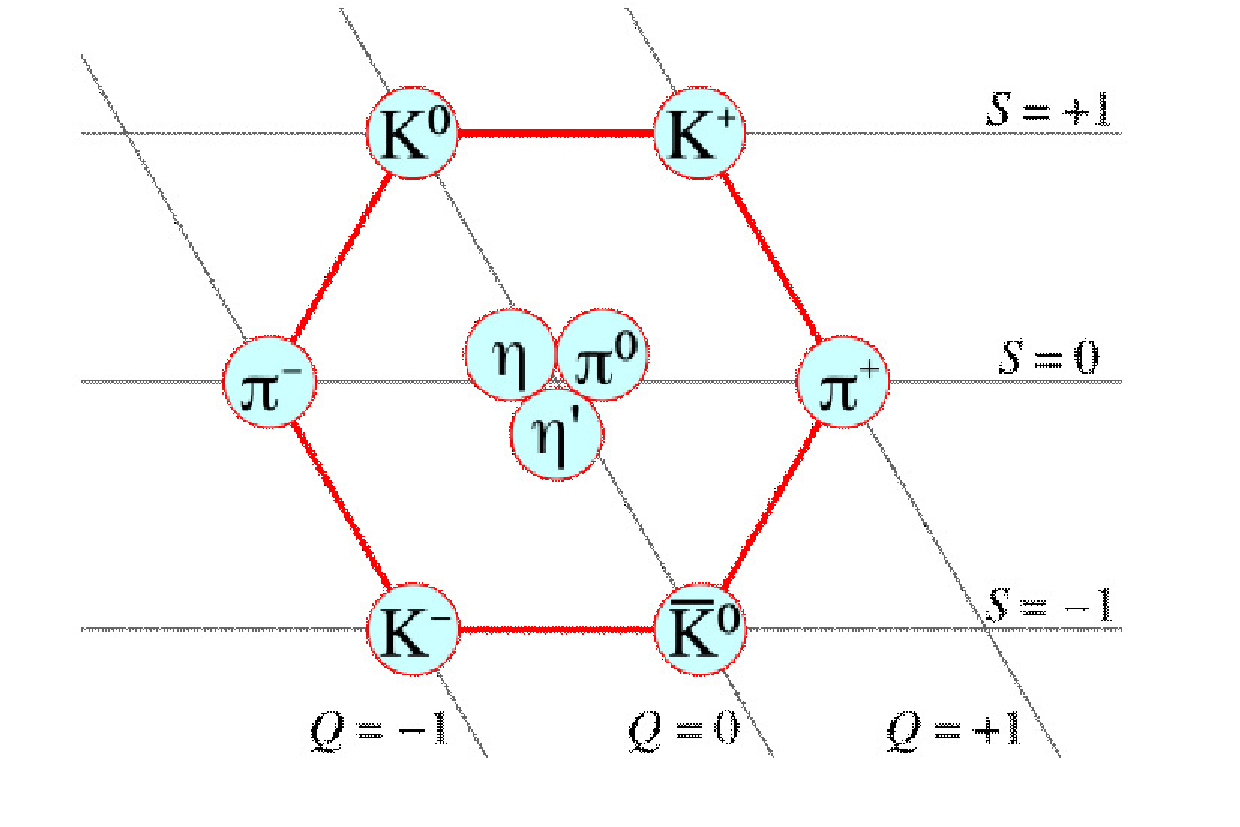
\includegraphics[width= 0.8 \figwidth ,height=\qfigheight]{\grpath/intro/pseudoscalar.pdf}
\caption[Nonet of Pseudoscalar Mesons]{\label{fig:nonet.pseud}Nonet of Pseudoscalar Mesons~\cite{wiki1}.}
\end{center}\end{figure}
It should be noted that the $\eta$ and $\eta'$ are not exact octet ($\eta_{8}$) and singlet ($\eta_{0}$) states, as they are linear combinations of $\eta_{8}$ and $\eta_{0}$ according to:
\begin{eqnarray}
\left(
\begin{array}{cc}
\eta \\
\eta ' 
\end{array}
\right)
& = &
\left(
\begin{array}{cc}
-\sin\theta_{mix} & \cos\theta_{mix} \\
\cos\theta_{mix} & \sin\theta_{mix}
\end{array}
\right)
\cdot
\left(
\begin{array}{cc}
\eta_{0} \\
\eta_{8}
\end{array}
\right)
\end{eqnarray}
where $\theta_{mix} = -18.6^{\circ}$\cite{Goity} and $\eta_{8}$ and $\eta_{0}$  have quark content of:
\begin{eqnarray}
\eta_{0} &\rightarrow & \sqrt{\frac{1}{6}}(u\overline{u} + d\overline{d} +  s\overline{s})\nonumber\\
\nonumber \\
\eta_{8} &\rightarrow & \sqrt{\frac{2}{3}}(u\overline{u} + d\overline{d} - 2s\overline{s})\nonumber \\
\nonumber \\
\nonumber 
\end{eqnarray}
The physical masses of $\eta$ and $\eta'$ are $m_{\eta} = 547.51\pm 0.18$~MeV \cite{pdg2014}, $m_{\eta'} =957.78 \pm 0.14$~MeV \cite{pdg2014}, and the widths are $\Gamma_{\eta} =1.30\pm0.07$~keV and $\Gamma_{\eta'} = 0.203\pm0.016$~MeV.
The lightest of the mesons $\pi^{0}$ has a quark content of:
\begin{eqnarray}
\pi^{0} = \frac{1}{\sqrt{2}}(u\overline{u} - d\overline{d})\nonumber
\end{eqnarray}
and mass of $m_{\pi^{0}} = 134.9766 \pm 0.0006$~MeV \cite{pdg2014}. The decay modes for \piz are given in Table \ref{tab:pi0}.
\begin{table}
\begin{minipage}{\textwidth}
\begin{center}
\begin{singlespacing}

\caption[Branching Ratios of the \piz Decay]{\label{tab:pi0} Branching ratios of the \piz decay.~\cite{pdg2014}}
\begin{tabular}{l|c}
\hline												
Mode	& Branching ratio \\ \hline 	
$\pi^0 \to 2\gamma$	 &   $ (98.823 \pm 0.034)  \cdot 10^{-2}$ \\	
$\pi^0 \to e^+ e^-\gamma$  &  $  (1.174 \pm 0.035)  \cdot 10^{-2}$ \\
$\pi^0 \to \gamma $ positronium   &  $ (1.82 \pm 0.29)  \cdot 10^{-9}$\\
$\pi^0 \to  e^+ e^+ e^- e^-	$  &  $( 3.34 \pm 0.16)  \cdot 10^{-5}$\\
$\pi^0 \to  e^+ e^-$  &  $ (6.46 \pm 0.33)  \cdot  10^{-8}$\\
$\pi^0 \to 4\gamma$	&  $<2 \cdot 10^{-8}$\\
$\pi^0 \to \nu \bar \nu$  &  $<2.7 \cdot 10^{-7}$\\
$\pi^0 \to \nu_e \bar \nu_e$  &  $<1.7 \cdot 10^{-6}$\\
$\pi^0 \to \nu_{\mu} \bar \nu_{\mu}$  &  $<1.6 \cdot 10^{-6}$\\
$\pi^0 \to \nu_\tau \bar \nu_\tau $  &  $<2.1 \cdot 10^{-6}$\\
$\pi^0 \to \gamma \nu \bar \nu$	 &  $<6 \cdot 10{-4}$\\
\hline \hline%inserts single line
\end{tabular}

\end{singlespacing}
\end{center}
\end{minipage}
\end{table}
\vspace{20pt}

%\begin{figure}[h!]\begin{center}
%\subfloat[Nonet of Pseudoscalar Mesons][]{ %Feynman diagram of \piz two photon decay
%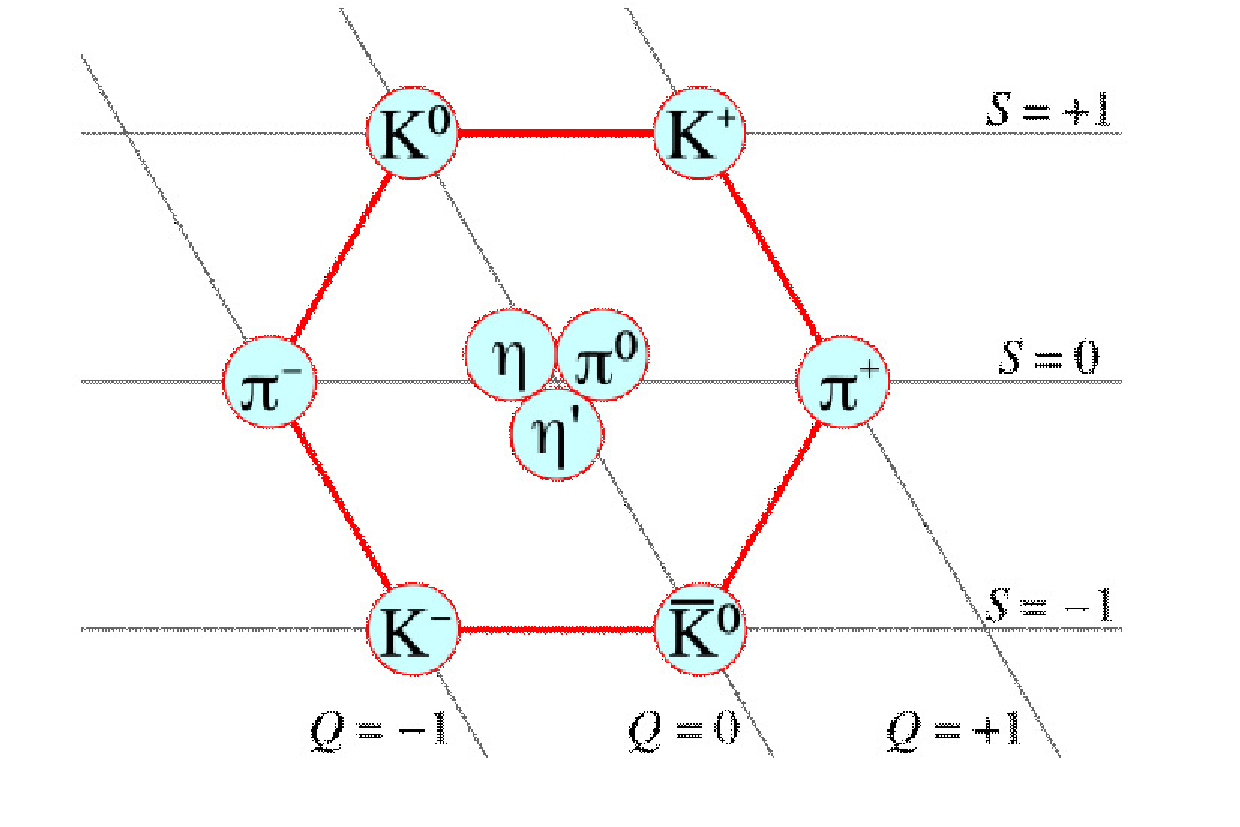
\includegraphics[width=0.65\columnwidth,height=0.5\qfigheight]{\grpath/intro/pseudoscalar.pdf}\label{fig:nonet.pseud}
%}
%
%\subfloat[Nonet of Vector Mesons][]{ %Feynman diagram of \piz Dalitz decay
%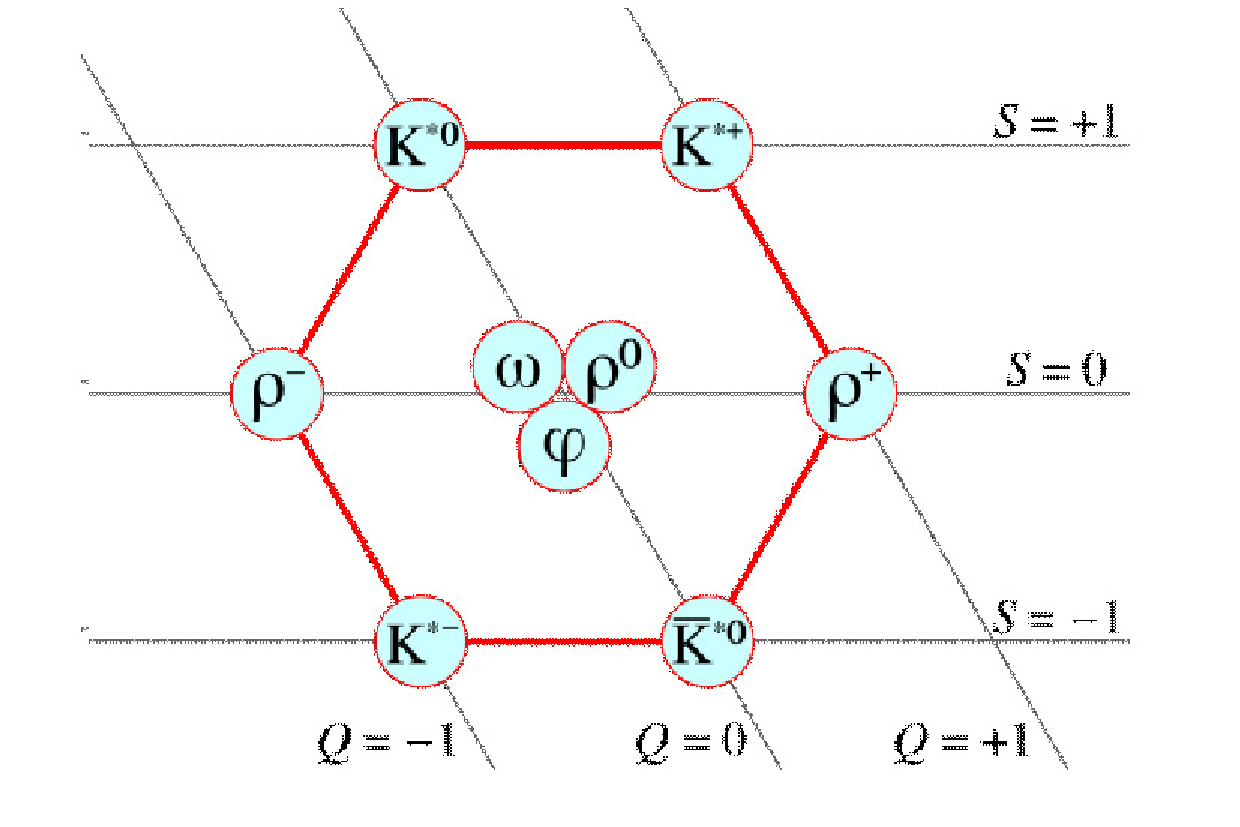
\includegraphics[width=0.65\columnwidth,height=0.5\qfigheight]{\grpath/intro/vector.pdf}\label{fig:nonet.vect}
%}
%\caption[Nonet of Pseudoscalar and Vector Mesons]{\label{fig:piz.alldecay}Nonet of pseudoscalar mesons~\subref{fig:nonet.pseud}. Nonet of vector mesons~\subref{fig:nonet.vect}.}
%
%\end{center}\end{figure}
%
%The \piz is the lightest meson with a mass of $m_{\pi^0}= (134.9766 \pm 0.0006) {\rm MeV}$ \cite{pdg2014}. The quark content is:
%\begin{equation}
% \pi^0 : \frac{1}{\sqrt{2}}\left(u \bar u  - d \bar d \right).
%\end{equation}

%In the intended analysis, it is planned to investigate the cross-section of the \piz.

\section{\piz Production} \label{sec:into:xsection}
The present analysis uses two approaches to describe the behavior of the \piz cross-section. One approach is for incident photon beam energies less than 2.8~GeV where the missing resonance search is most valid and the data can be described well by coupling of the \piz electromagnetic wave functions. The second approach attempts to describe the behavior of the \piz by using General Parton Distribution models, \abbr{GPD} for incident photon beam energies greater than 2.8~GeV.
%The physics behind this is that since the photon couples to charged-fermion pairs, a part of its cross-section could be described by considering interactions between the hadron and a virtual fermion pair~\cite{butterworth}.


\subsection{Low Energy \piz Production}\label{sec:into:xsection.low}

\begin{figure}[h!]\begin{center}
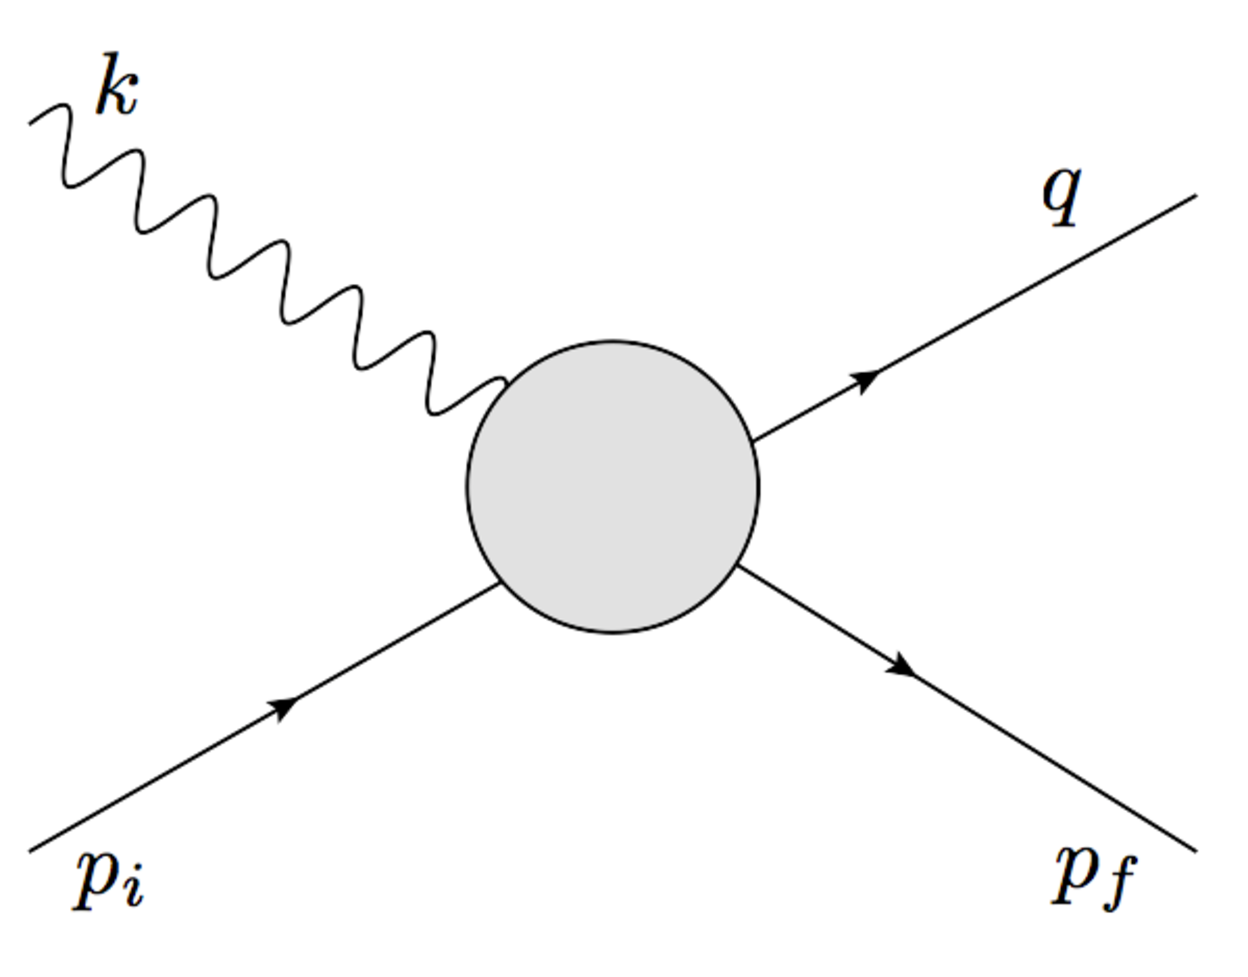
\includegraphics[width=0.5 \figwidth,height= \qfigheight]{\figures/feyman_pi0IV.pdf}
\caption[Diagram for photoproduction of the \piz meson]{\label{fig:xsection.pi0feynman}	Diagram for photoproduction of the \piz meson. $k$ and $p_i$ are the incident photon beam and target proton 4-moment respectively, $q$ and $p_f$ represent the produced \piz meson and scattered proton 4-momenta respectively.}
\end{center}\end{figure}
For incoming photon beam energies less than 2.8~GeV, the production of the \piz meson, with 4-momenta $q$, in photon-proton reactions, with 4-momenta $k$ and $p_i$ respectively and $p_f$ being the 4-momenta of the scattered proton (see Fig.~\ref{fig:xsection.pi0feynman}),  can be described in terms of the three Lorentz invariant Mandelstam variables, $s$, $t$ and $u$, where
\begin{align}
s = (k+p_i)^2 = (q+p_f)^2 \nonumber \\
t=(p_i-p_f)^2 = (k-q)^2  \nonumber \\
u = (k - p_f)^2 = (p_i-q)^2 \ .
\end{align}
The sum of the Mandelstam variables linearly combine to give the sum of masses of the particles involved:
\begin{align}
s + t + u = \sum\limits_{i}^{4} m_i^2 
\end{align}
and the definition of Lorentz-invariant mass:
\begin{align}
p_i\cdot p_i = E_i^2 - \mathbf{p_i}\cdot \mathbf{p_i} = m_i^2 \ .
\end{align}
Using energy-momentum conservation:
\begin{align}
k + p_i = q+p_f \,
\end{align}
it is seen that only three of the four momenta are independent. Conventionally the use of $k$ and $q$ and a combined 4-momenta of the nuclei 
\begin{align}
P = \frac{1}{2}(p_i+p_f)
\end{align}
are used as the independent kinematic variables. The three Mandelstam variables can be express in terms of the other two, therefore the scattering process is described by functions of only two of the Mandelstam variables. Conventionally they are chosen to be $s$ and $t$, which in the center-of-mass frame (C.M.) of the initial and final state equal the invariant mass squared of the system and the momentum transfer in the production process respectively.
\subsection{Isospin Representation}\label{sec:isospin}
The scattering matrix $\mathcal{M}$ for single pion photoproduction process is written as:
\begin{align}
\mathcal{M} =  (\epsilon_\mu k_\nu - \epsilon_\nu k_\mu)&[ \frac{1}{2}i \gamma_5 \gamma_\mu \gamma_\nu A_1(s,t) + 2 i \gamma_5 P_\mu(q-\frac{1}{2}k)_\nu A_2(s,t) \nonumber \\ & + \gamma_5 \gamma_\mu q_\nu A_3(s,t) + \gamma_5 \gamma_\mu(2P_\nu- i M\gamma_\nu) A_4(s,t) ] \ ,
\end{align}
where $M$ is the nucleon mass, $\epsilon$ is the photon polarization and $A_i(s,t)$ are the invariant functions of the Mandelstam invariants $s$ and $t$. The amplitude $A_i(s,t)$ refers to the emission of a pion of isospin index $\alpha$, and is given by the well-known formula:
\begin{align}\label{eq:isoscal_vec}
A_i(s,t)= A_i^{(0)}\tau_\alpha + A_i^{(+)}\delta_{\alpha 0} + \frac{1}{2} A_i^{(-)}\left[\tau_\alpha,\tau_0\right] \ ,
\end{align}
where $\tau_\alpha$ are the nucleon isospin transition operators, where the sign of $\alpha$ indicates the opposite sign of the pion isospin, this is by convention. Eq.~\ref{eq:isoscal_vec} assumes that the photon interaction with hadrons occurs through isoscalar and isovector parts, so that $A_i^{(0)}$ is the isoscalar amplitude that corresponds to a zero net isospin transistion resulting from the electromagnetic field. The amplitudes $A_i^{(+)}$ and $A_i^{(-)}$ are the isovector amplitudes and can be combined as $A_i^{(+)} + 2 A_i^{(-)}$ and $A_i^{(+)} - A_i^{(-)}$ so that the pion nucleon final state has definite isospin $\frac{1}{2}$ and $\frac{3}{2}$ respectively~\cite{Rosenfeld} by use of
\begin{align}
A^S = -(3)^\frac{1}{2}A^{(0)} \nonumber \\
A^{V1} = \left(\frac{1}{3}\right)^\frac{1}{2}A_i^{(+)} + 2 A_i^{(-)} \nonumber \\
A^{V2} = \left(\frac{2}{3}\right)^\frac{1}{2}A_i^{(+)} - A_i^{(-)} \ ,
\end{align}
where $A^S$, $A^{V1}$ and $A^{V2}$ are the isoscalar amplitude, isovector amplitude of isospin $\frac{1}{2}$ and isovector amplitude of isospin $\frac{3}{2}$ respectively.
The four possible pion nucleon amplitudes $A_i(s,t)$ of the initial and final state particles in the pion photoproduction process are in terms of the isoscalar and isovector are:
\begin{align}
A_1(\gamma p \to n \pi^+) = -\sqrt{\frac{1}{3}}A^{V3} + \sqrt{\frac{2}{3}}(A^{V1} - A^{S}),\\
A_2(\gamma p \to p \pi^0) = \sqrt{\frac{2}{3}} A^{V3} + \sqrt{\frac{1}{3}}(A^{V1}-A^{S}),\\
A_3(\gamma n \to p \pi^-) = \sqrt{\frac{1}{3}}A^{V3} - \sqrt{\frac{2}{3}}(A^{V1} + A^{S}),\\
A_3(\gamma n \to n \pi^0) = \sqrt{\frac{2}{3}}A^{V3} + \sqrt{\frac{1}{3}}(A^{V1} + A^{S}).
\end{align}
Since the combination $\sqrt{\frac{2}{3}}(A^{V1} \mp A^{S})$ gives the coupling of photons to positive and neutral isospin-$\frac{1}{2}$ states, respectively, ~\protect\cite{Rosenfeld}, defined explicitly
%
\begin{align}
&&A^p = + \sqrt{\frac{2}{3}}(A^{V1} - A^{S}),\\
&&A^n = -\sqrt{\frac{2}{3}}(A^{V1} + A^{S}).
\end{align}
\subsection{Structure Functions}\label{sec:CGLN}
To obtain the scattering matrix elements in terms of experimental quantities, it is preferred and easier to work in the C.M. system and reduce the $\mathcal{M}$ to a form $\mathcal{F}$ by equating the invariant form of the scattering matrix elements in each frame, i.e.:
\begin{align}
\bar{u}(p_2)\mathcal{M} u(p_1) \equiv \frac{4 \pi W}{M}\chi_f^\dagger \mathcal{F} \chi_i \ ,
\end{align}
where $\bar{u}(p_2)$ and $u(p_1)$ are final and initial state Dirac spinors respectively and $\chi_f$ and $\chi_i$ are final and initial state Pauli spinors. The differential cross-section for single pion production is:
\begin{align}
\frac{d\sigma}{d\Omega} = \frac{q}{k}| \bra{f}\mathcal F \ket{i}|^2,
\end{align}
The expression to express Dirac spinors in terms of Pauli spinors is written as:
\begin{align}
\mathcal{F} = & i\vec{\mathbf{\sigma}}\cdot \vec{\mathbf{\epsilon}} \mathcal{F}_1 + \frac{1}{qk}(\vec{\mathbf{\sigma}}\cdot \vec{\mathbf{q}})\vec{\mathbf{\sigma}} \cdot(\vec{\mathbf{k}}\times \vec{\mathbf{\epsilon}}) \mathcal{F}_2 \nonumber \\ & + \frac{i}{qk}(\vec{\mathbf{\sigma}}\cdot \vec{\mathbf{k}})(\vec{\mathbf{q}}\cdot \vec{\mathbf{\epsilon}})\mathcal{F}_3 + \frac{i}{q^2}(\vec{\mathbf{\sigma}}\cdot \vec{\mathbf{q}})(\vec{\mathbf{q}}\cdot \vec{\mathbf{\epsilon}})\mathcal{F}_4 \ ,
\end{align}
where $\vec{\mathbf{k}}$ and $\vec{\mathbf{q}}$ are the C.M. 3-momenta and $\vec{\mathbf{\epsilon}}$ is the polarization of the photon. The relationship between $A_i$ and $\mathcal{F}$ is found using the relations:
\begin{align}
\mathcal{F}_1 = \frac{W- M}{8 \pi W }(D_1 D_2)^{\frac{1}{2}}\left[ A_1+(W-M)A_4 - \frac{k_0q_0-\vec{\mathbf{k}}\cdot \vec{\mathbf{q}}}{W-M}(A_3-A_4)\right] \\
\mathcal{F}_2 = qk \frac{W- M}{8 \pi W }(\frac{D_2}{D_1})^{\frac{1}{2}}\left[ -A_1+(W+M)A_4 + \frac{k_0q_0-\vec{\mathbf{k}}\cdot \vec{\mathbf{q}}}{W+M}(A_3-A_4)\right]  \\
\mathcal{F}_3 =qk \frac{W- M}{8 \pi W }(D_1 D_2)^{\frac{1}{2}}q\left[(W-M)A_2 + A_3 - A_4\right]\\
\mathcal{F}_4 = q^2 \frac{W- M}{8 \pi W }(\frac{D_2}{D_1})^{\frac{1}{2}}q\left[ -(W+M)A_2 + A_3 - A_4\right] 
\end{align}
where
\begin{align}
D_1 = (M^2 + \vec{\mathbf{k}}^2)^{\frac{1}{2}}+M \\
D_2 = (M^2 + \vec{\mathbf{q}}^2)^{\frac{1}{2}}+M \ .
\end{align}
$\mathcal{F}_i(s,t)$ are known as structure functions, alternatively known by Chew, Goldberger, Low and Nambu (\abbr{CGLN}) amplitudes. These amplitudes describe photoproduction as a function of $s$ and $t$, and therefore in terms of momentum transfer. To represent the process in terms of angular momentum transitions, expansion of the structure functions as partial waves in derivatives of Legendre polynomials, $P_l^\prime(\cos\theta)$, results in the four multipole series:
\begin{align}
&&\mathcal{F_1} = \displaystyle\sum_{l=0}^{\infty}[lM_{l+} + E_{l^+}]P_{l+1}^{\prime}(\cos\theta) + [(l+1)M_{l-1} + E_{l-}]P_{l-1}^{\prime}(\cos\theta)\\
&&\mathcal{F_2} = \displaystyle\sum_{l=1}^{\infty}[(l+1)M_{l+}+lM_{l-}]P_{l}^{\prime}(\cos\theta)\\
&&\mathcal{F_3} = \displaystyle\sum_{l=1}^{\infty}[E_{l+}-M_{l+}]P_{l+1}^{\prime \prime}(\cos\theta) + [E_{l-} + M_{l-}]P_{l-1}^{\prime \prime}(\cos\theta)\\
&&\mathcal{F_4} = \displaystyle\sum_{l=1}^{\infty}[M_{l+} - E_{l+} - M_{l-} - E_{l-}]P_{l}^{\prime \prime}(\cos\theta)
\end{align}
The energy-dependent amplitudes $M_{l\pm}$ and $E_{l\pm}$ refer to transitions initiated by magnetic and electric radiation, respectively, leading to final states of orbital angular momentum $l$ and total angular momentum $j=l\pm\frac{1}{2}$. 

The energy-dependent amplitudes $M_{l\pm}$ and $E_{l\pm}$ cannot be extracted directly from measurements, however using models on measured differential cross-sections and polarizations aide in the determination of the amplitudes. Constraining the production amplitudes aides in the determination of resonances. One such model that is used in this thesis is the SAID parameterization model discussed in Sec~\ref{sec:intro.said}. 


\subsection{SAID}\label{sec:intro.said}

SAID~\cite{SAID} is a repository of experimental data and an interactive analysis facility, allowing to compare and extract data and partial wave solutions (PWA) for a variety of photoproduction, electro-production and pion production reactions. It was created by R. A. Arndt and L. D. Roper for the use of verifying model calculations against measured/fitted data, compare model calculations against SAID predictions for unmeasured observables, experimental planning, and simulations and event generators.

SAID is based upon the theoretical framework given in~\ref{sec:isospin}. SAID generates resonance couplings, in terms of angular momentum and isospin quantum numbers, that are extracted from a fit-based determination of multipoles using both an energy-dependent and an energy-independent parametrization. The photoproduction amplitude is assumed to be in the form of a Breit-Wigner and a background term in the form of~\cite{ar90};
\begin{align}
A=A_l(1+iT_\pi)=A_r\left(\frac{k_0q_0}{kq}\right)^{\frac{1}{2}} \frac{W_0\sqrt{\Gamma \Gamma_{\gamma}}}{W_0^2-W^2-iW_0\Gamma} \ ,
\end{align}
in which $A_l$ is the background parameter, $W_0$, $\Gamma$ and $\Gamma_{\gamma}$ are functions of the full width $\Gamma_{0}$ and $A_R$ being the resonant parameter in the form of;
\begin{align}
A_r=\frac{\mu}{q}\left(\frac{k}{q}\right)^l\sum_{n=0}^{N}p_n\left(\frac{E_{\pi}}{\mu}\right)^n
\end{align}
where $k_0$ and $q_0$ are the pion and photon momenta at the resonance energy, $\mu$ is the pion mass, $E_{\pi}$ is the pion kinetic energy in the lab frame and $p_n$ is a free parameter. The background term is expanded as a set of Legendre polynomial terms with associated free parameters along with a sum of a pseudoscalar Born partial waves, which are determined by fitting the data. Multipoles can then be extracted by a fit of $A$ close to the resonance position.

\subsection{Summary}
A full set of differential cross-sections and polarization observables is required for the determination of multipoles. These can be related to the invariant amplitudes as functions of $W$ and $\cos\theta$. For the separation of the different isospin contributions, both the proton and the neutron pion-photoproduction measurements are needed. An understanding of the invariant amplitudes, and subsequent CGLN structure functions, can provide information on the multipole transitions taking place. This  allows to get direct information about the quantum numbers of the produced resonant states and constrain their position, widths and couplings.
The work of this thesis is devoted to measuring of the differential cross-sections for better fit determinations and possible resonance searches using the SAID parameterizations.
\subsection{High Energy \piz Production}\label{sec:into:xsection.high}
%ere is the citation ~\cite{key1, key2,Rad1996, Diehl}
The production of the \piz meson in photon-proton reactions, for incoming photon beam energies greater than 2.8~GeV, is considered to be a hard exclusive reaction. One approach to study the \piz production, in photon-proton reactions, is use the handbag model. In the handbag approach, the reaction is factorized into two parts. The first part is when one quark from the incoming and one from the outgoing nucleon participate in the hard sub-process, small blob in Fig.~\ref{fig:xsection.handbag}. This hard sub-process is achieved when the incident photon excites a quark, since quarks are bound quantum particles, the excited quark produces a jet of quarks that form the meson and then de-excites back into the nucleon. This is calculable using pQCD. The second part ,the soft part seen as the large blob in Fig.~\ref{fig:xsection.handbag} , consists of all the other quarks that are spectators and can be described in terms of GPDs~\cite{key1, key2,Rad1996, Diehl}. The hard exclusive meson (M) photo-production process factorizes into, $\gamma q \to Mq$, this is depicted in Fig.~\ref{fig:xsection.handbag}. The handbag mechanism is applicable when the Mandelstam variables, $s$, $t$, $u$, are large as compared to a hadronic scale of order 1 GeV . In Ref.~\cite{Huang2000} a model, derived from the handbag approach, has been applied to predict angular dependence of scaled photoproduction cross section of \piz and is illustrated in Fig.~\ref{fig:xsection.handbag.cal}. In the analysis presented, this model will investigated using the data obtained in \abbr{CLAS}.

\begin{figure}[h!]\begin{center}
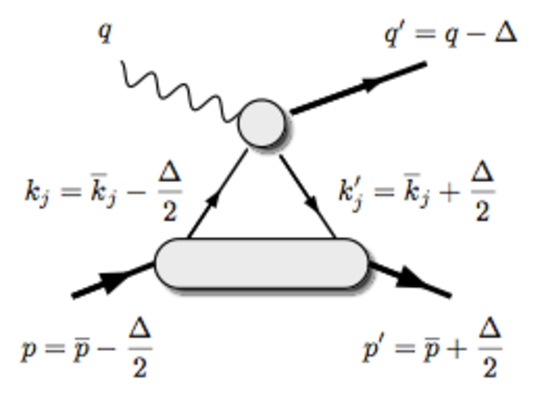
\includegraphics[width= 0.8 \figwidth ,height=\qfigheight]{\grpath/intro/handbag.pdf}
\caption[The handbag-type diagram for photoproduction of mesons]{\label{fig:xsection.handbag}	The handbag-type diagram for photoproduction of mesons. The large blob represents a sum over all spectator configuration. $k_j$ and $k_j^{\prime}$  denote the momenta of the active partons. The small blob stands for meson photoproduction off partons.}
\end{center}\end{figure}

\begin{figure}[h!]\begin{center}
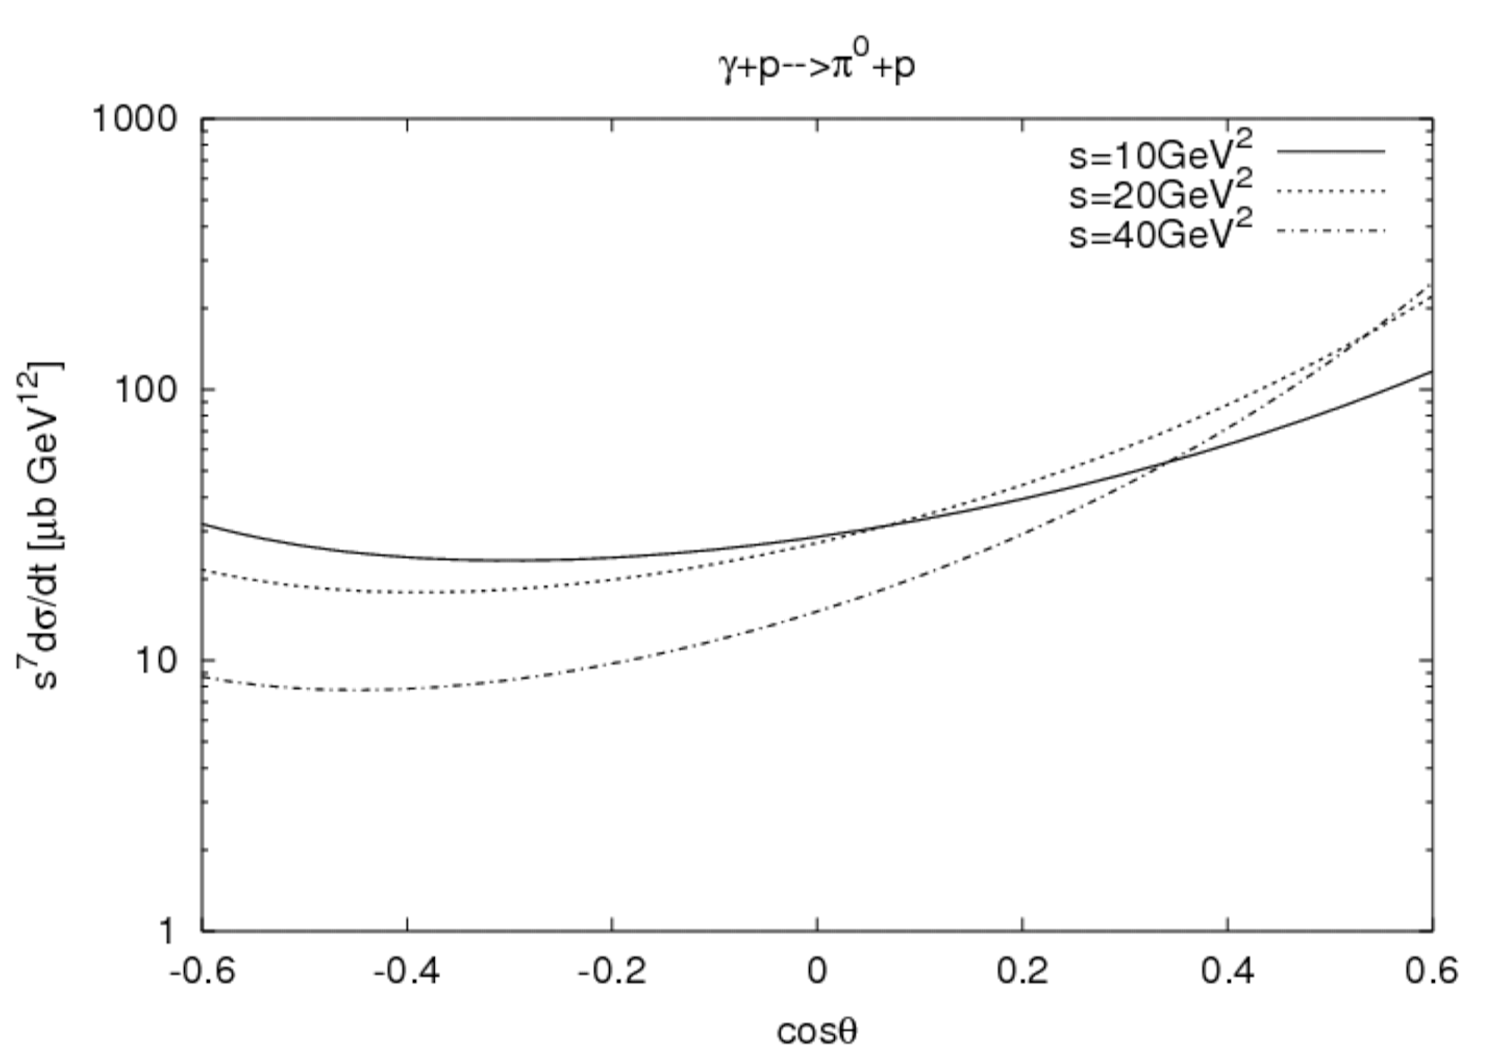
\includegraphics[width= 0.8 \figwidth ,height=\qfigheight]{\grpath/intro/photo-fig7.pdf}
\caption[The soft physics contribution to the cross-section for photoproduction of \piz]{\label{fig:xsection.handbag.cal}The soft physics contribution to the cross-section for photoproduction of \piz scaled by s$^7$ versus $\cos\theta$, where $\theta$ is the scattering angle in the $\gamma p$ c.m. system~\cite{Huang2000}.}
\end{center}\end{figure}
\FloatBarrier


% %
\section{\piz Decays}\label{sec:intro.decays}
The main decays studied for this analysis are when a pseudoscalar meson, $P_p$($\pi^{0}$, $\eta$, $\eta'$), decays via 2 photons $\gamma \gamma$ or a photon $\gamma$ and a dilepton ($l^{+}l^{-}$) pair, which are the two most prevalent decays of \piz as shown in Table~\ref{tab:pi0}. Figure~\ref{fig:piz.alldecay} illustrates the Feynman diagrams for the ``Two photon decay'' and the ``Dalitz decay''.
\begin{figure}[h!]\begin{center}
\subfloat[Feynman Diagram of \piz Two Photon Decay][]{ %Feynman diagram of \piz two photon decay
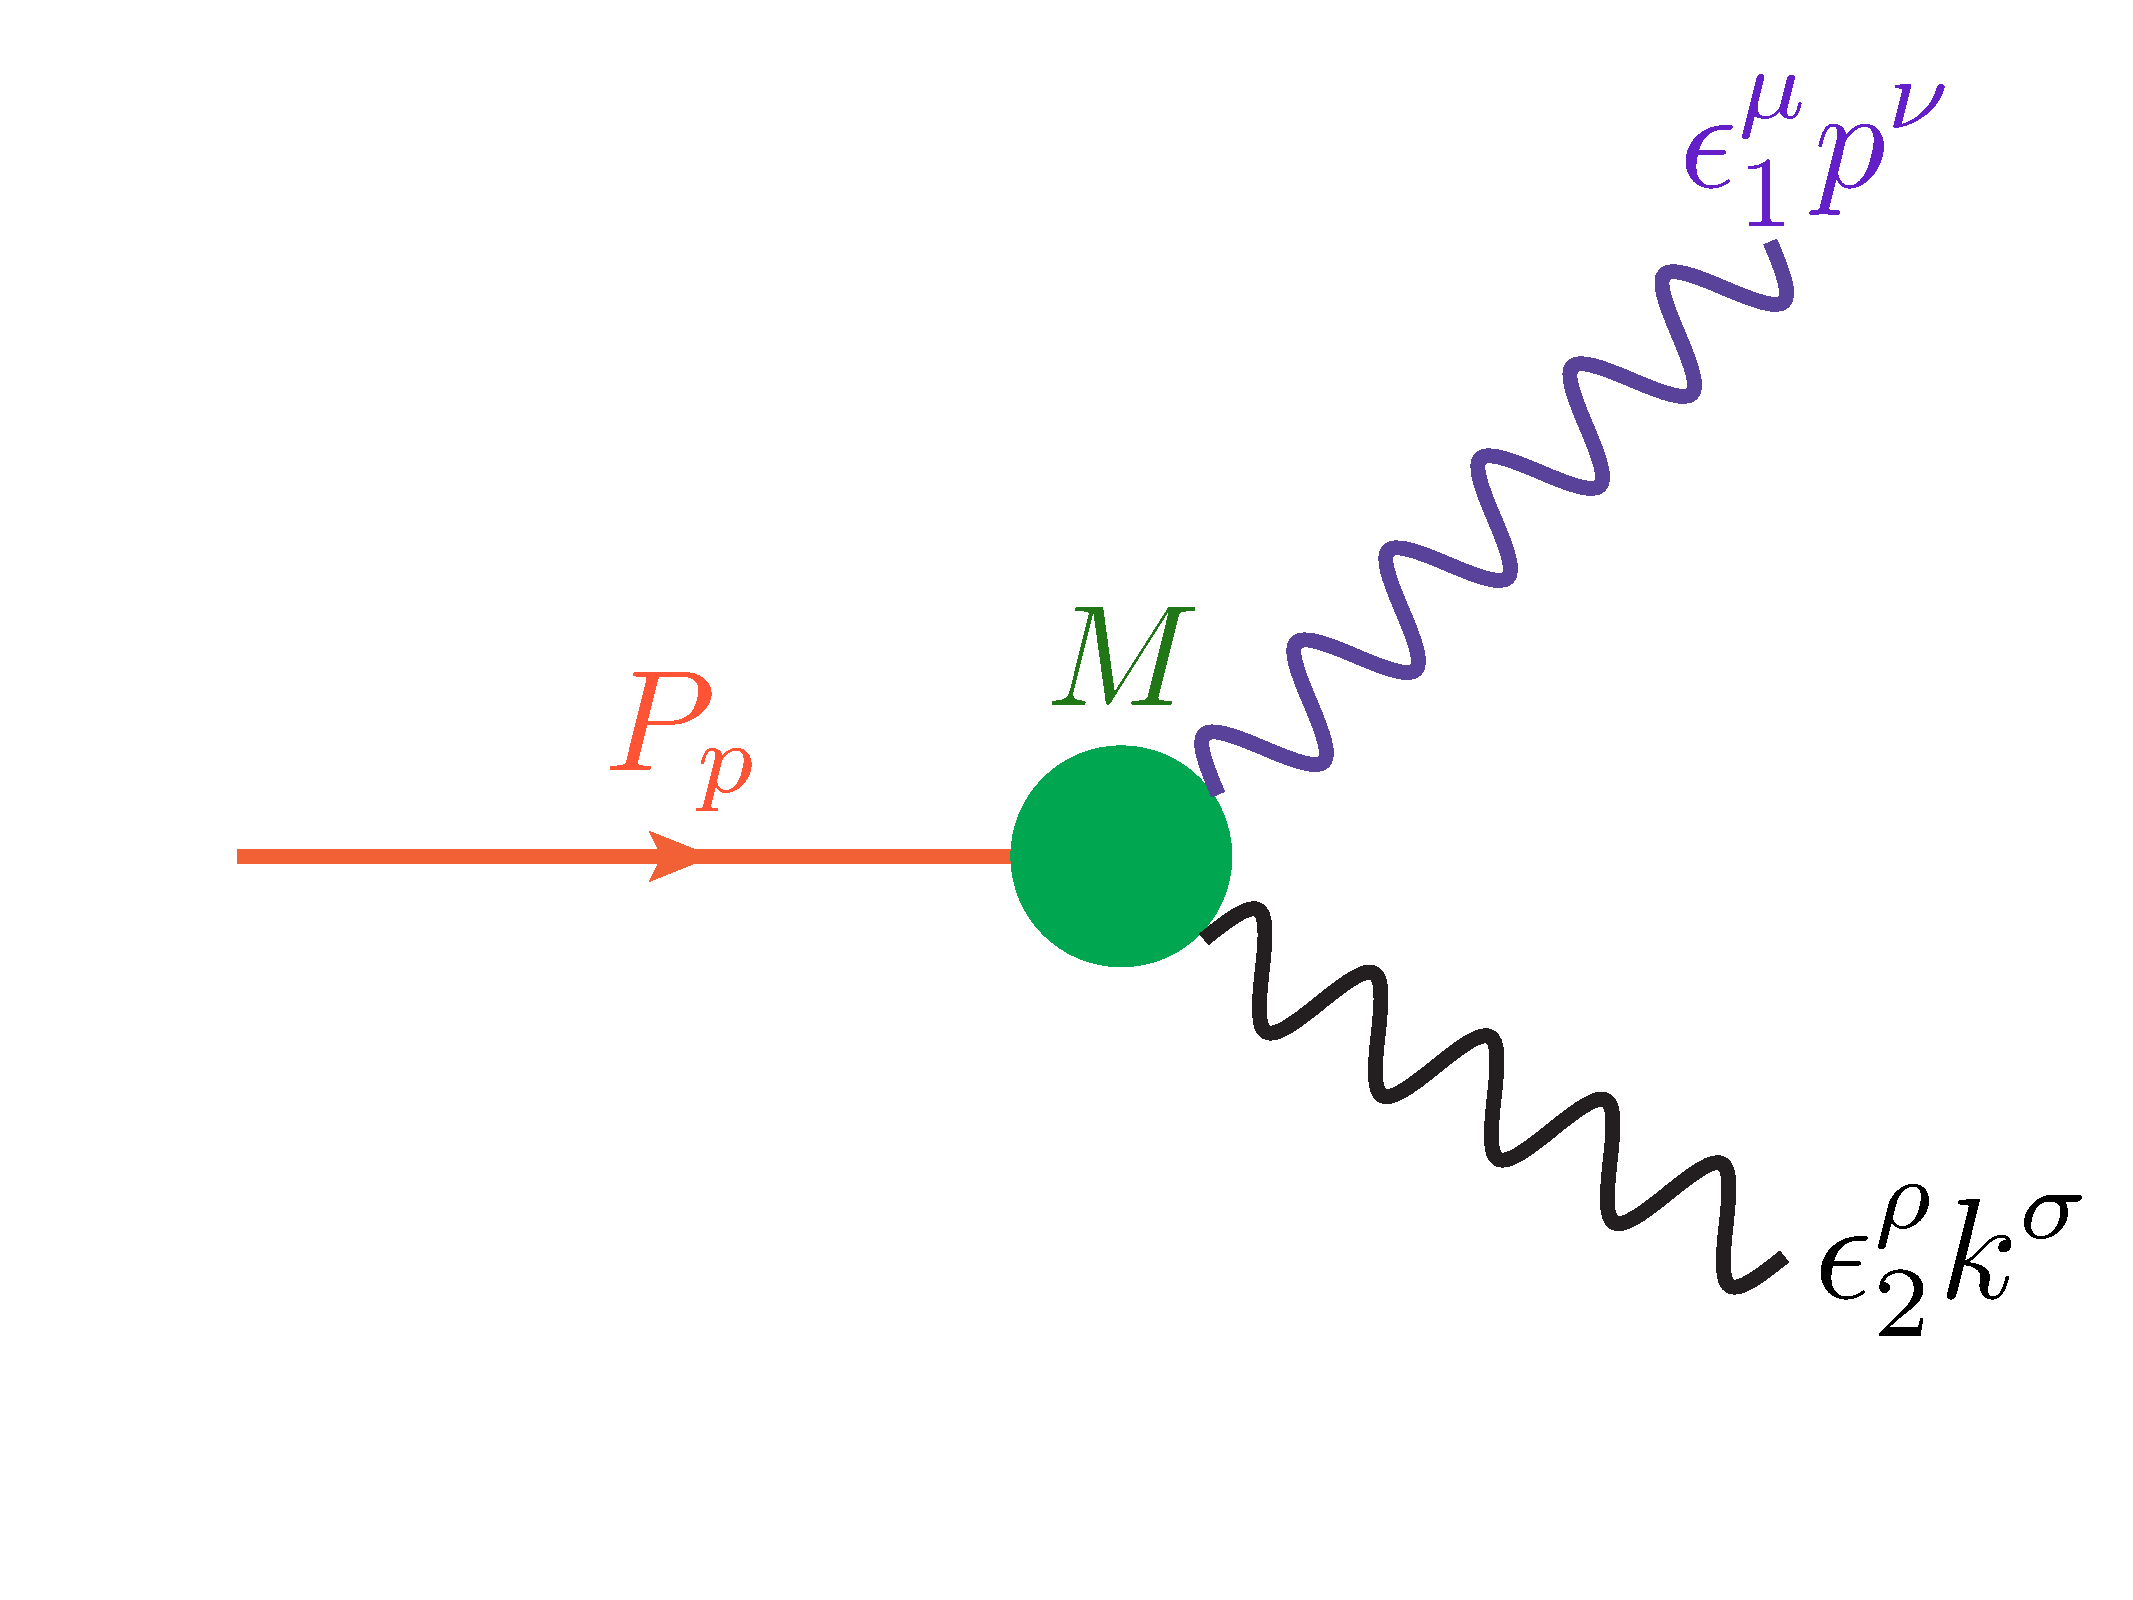
\includegraphics[width=0.65\columnwidth,height=0.5\qfigheight]{\grpath/intro/decays/P_to_gamgam_wnotation.pdf}\label{fig:piz.gamgam}
}

\subfloat[Feynman Diagram of \piz Dalitz Decay][]{ %Feynman diagram of \piz Dalitz decay
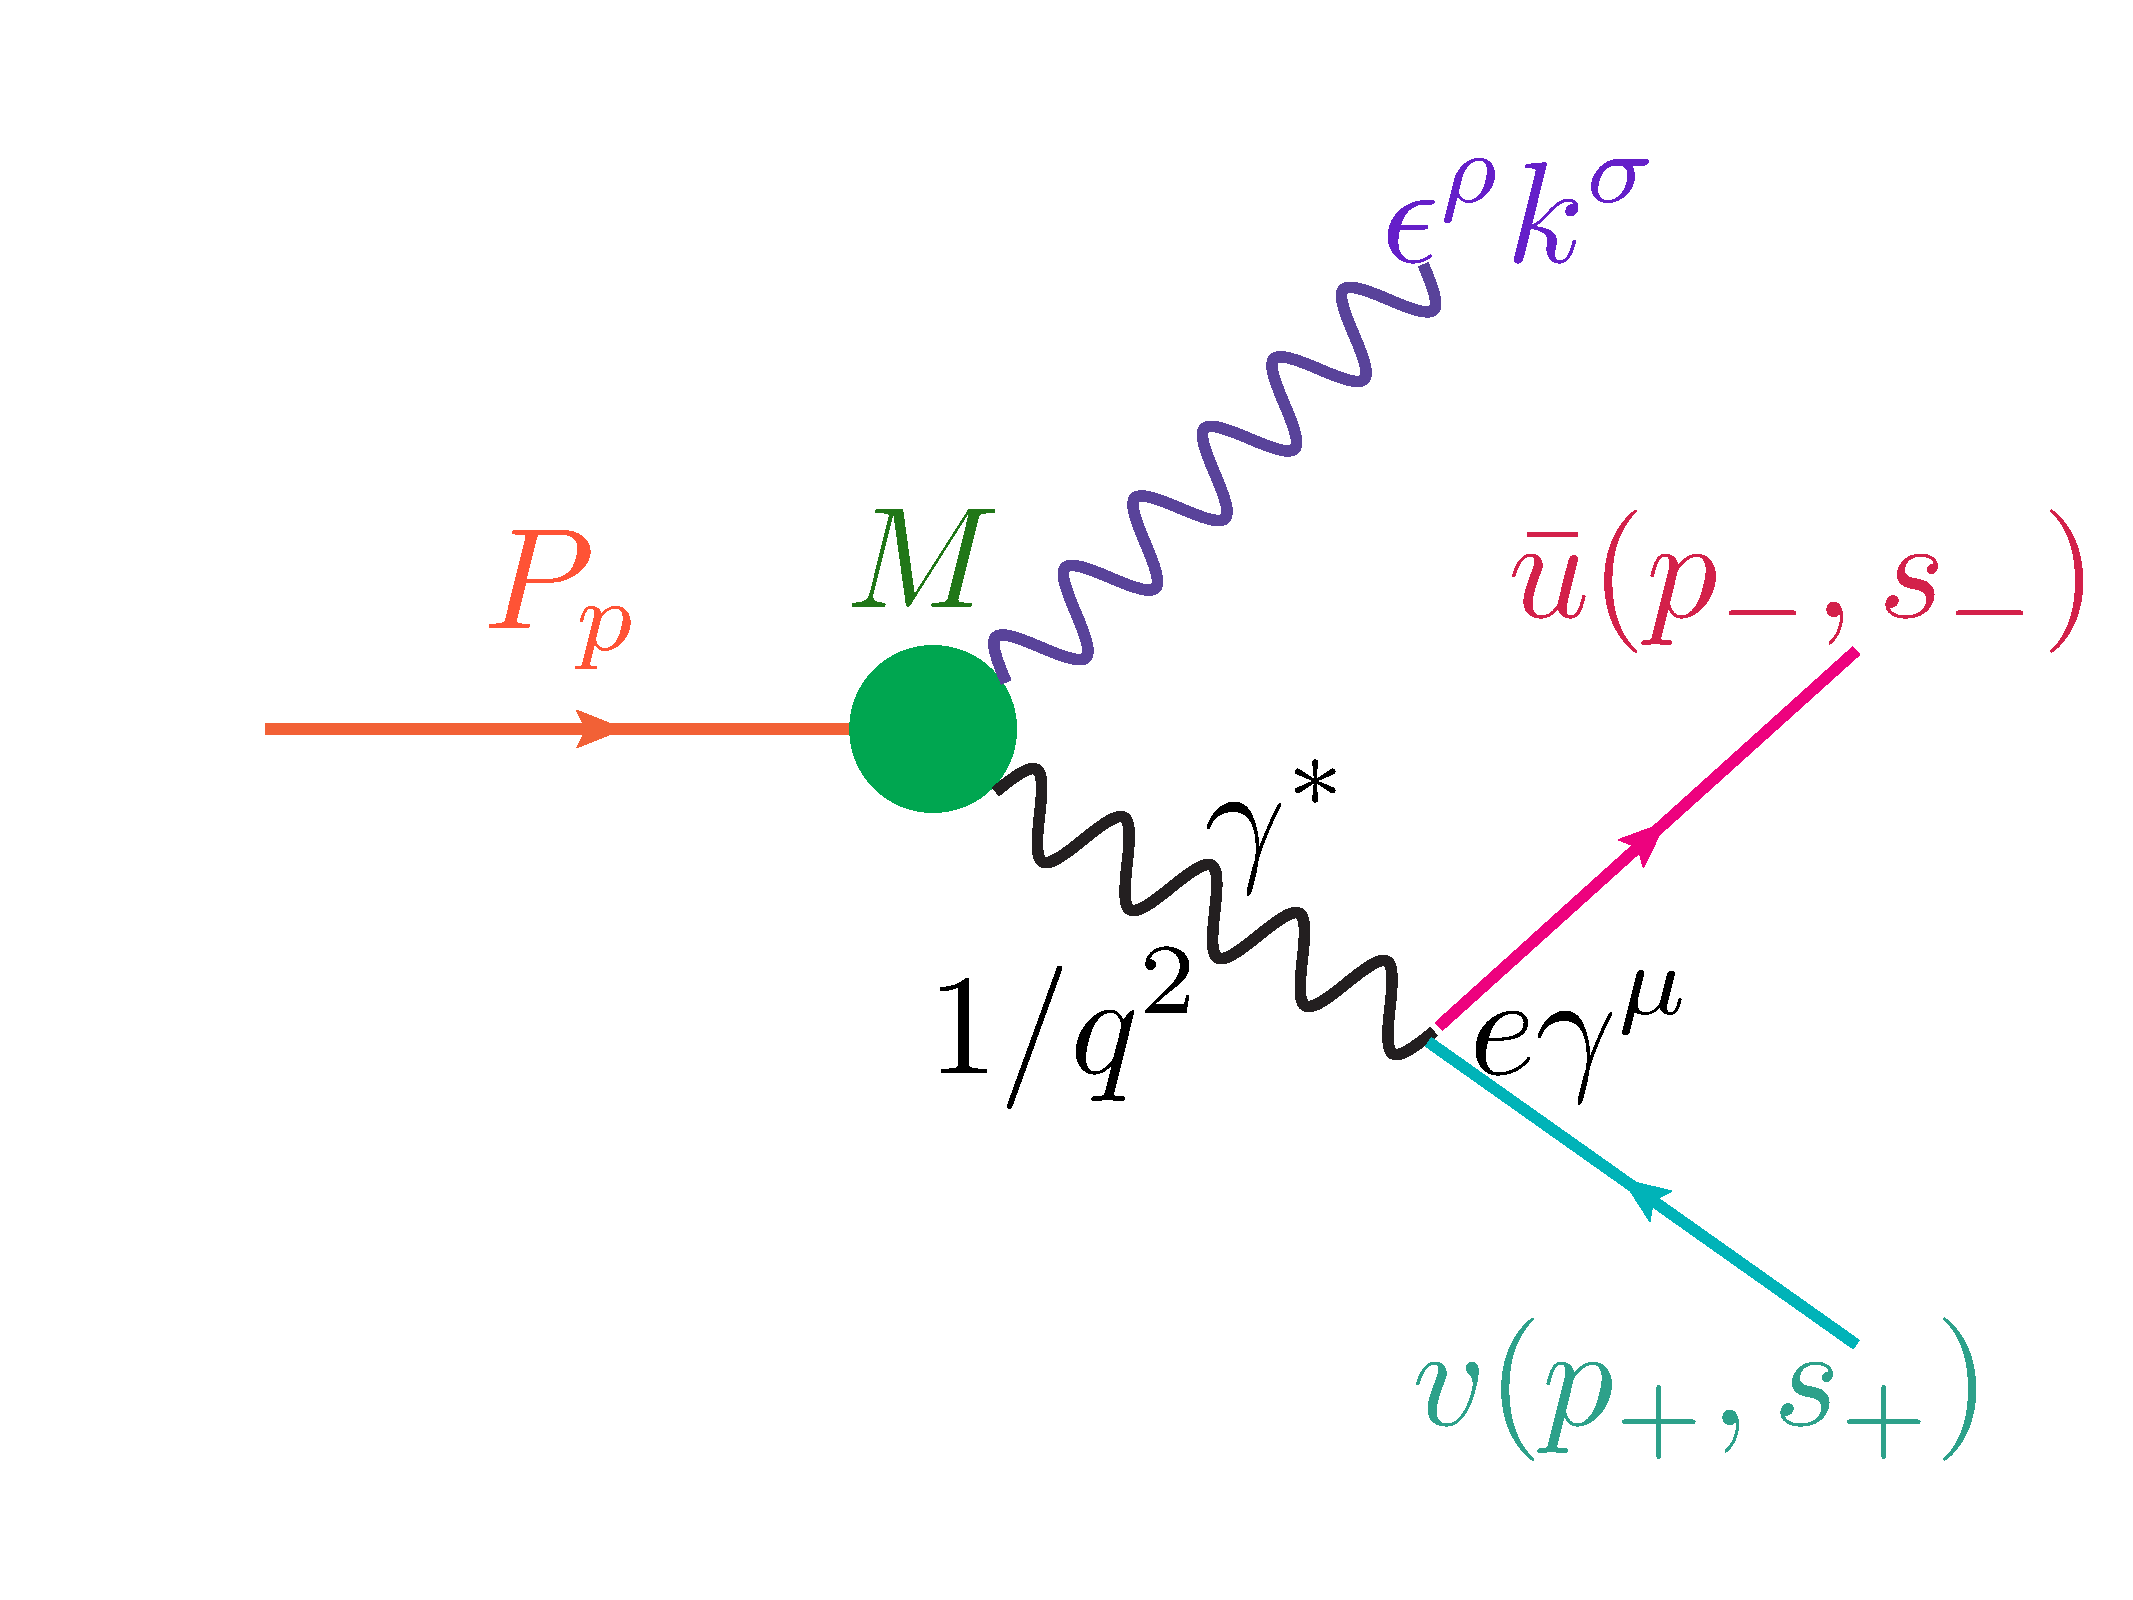
\includegraphics[width=0.65\columnwidth,height=0.5\qfigheight]{\grpath/intro/decays/P_to_lepsgam_wnotation.pdf}\label{fig:piz.dalitz}
}
\caption[Feynman diagram of $P_p$($\pi^0$) two photon decay and Dalitz decay]{\label{fig:piz.alldecay}Feynman diagram of $P_p$($\pi^0$) two photon decay~\subref{fig:piz.gamgam}, $\epsilon_1$ and $\epsilon_2$ are the polarizations, $p$ and $k$ are 4-momenta of the photons.  Feynman diagram of $P_p$($\pi^0$) Dalitz decay~\subref{fig:piz.dalitz}, the variable $s_\pm$ are the spin helicities of the outgoing leptons $l^\pm$ with 4-momenta $p_{\pm}$ and $\epsilon$ is the polarization of the outgoing photon with 4-momenta $k$. In both diagrams $\mathcal{M}$ is the form factor.}

\end{center}\end{figure}
\FloatBarrier
\subsection{Two Photon Decay}\label{sec:piz.gg}
As shown in Fig.~\ref{fig:piz.gamgam}, the two photon decay can be expressed in terms of the respective momentum, $P_p$($\pi^0$)$\to \gamma(\epsilon_1,p) \gamma(\epsilon_2,k)$, where $\epsilon_1$ and $\epsilon_2$ are the polarizations of the photons with 4-momenta $p$ and $k$. Dropping the nomenclature ($\pi^0$) in $P_p$($\pi^0$), the four momentum of the decaying meson is $P_p= p+k$. Using the Feynman rules as given in~\cite{peskin}and~\cite{halzen}, which are Lorentz and gauge invariant and also parity conserving, the amplitude can be solved to be:
\begin{align}\label{eq:piz.gg.amp}
 {\cal M}(P_P \to \gamma(\epsilon_1,p) \gamma(\epsilon_2,k))= {M}_P(p^2=0,k^2=0) \varepsilon_{\mu\nu\rho\sigma}\epsilon_1^\mu p^\nu \epsilon_2^\rho k^\sigma
\end{align}
where $\varepsilon_{\mu\nu\rho\sigma}$ is the antisymmetric metric tensor. The form factor, ${M}_P(p^2=0,k^2=0)$, contains information of the decaying meson and since the decay products are on-shell photons, which are massless, ${M}_P$ is a constant given as;
\begin{align}\label{eq:decay.constants}
 {M}_P=\begin{cases}
         {\displaystyle\frac{\alpha}{\pi f_{\pi}}} & \mbox{if $P=\pi^0$};\\
        {\displaystyle\frac{\alpha}{\pi f_\pi} \frac{1}{\sqrt{3}} }\left( \frac{f_\pi}{f_8} \cos\theta_{mix} -2\sqrt{2} \frac{f_\pi}{f_0} \sin\theta_{mix} \right)& \mbox{if $P=\eta$};\\
        {\displaystyle\frac{\alpha}{\pi f_\pi} \frac{1}{\sqrt{3}}} \left( \frac{f_\pi}{f_8} \sin\theta_{mix} +2\sqrt{2} \frac{f_\pi}{f_0} \cos\theta_{mix} \right)& \mbox{if $P=\eta'$} \,
\end{cases}
\end{align}
where $\alpha=e^2/4\pi \approx 1/137$ is the fine structure constant, $f_\pi \approx 92.4 \,{\rm MeV}$ is the physical value of the pion-decay constant and $f_0 \approx 1.04 f_\pi$ and $f_8 \approx 1.3 f_\pi$ are the singlet and octet Pseudo-Goldstone meson decay constants.

\subsubsection{\emph{Squared Matrix Element}}
The squared matrix element of the decay $P_P \to \gamma(\epsilon_1,p) \gamma(\epsilon_2,k)$ is given by
\begin{align}\label{eq:piz.gg}
\left|{\cal  M}(P_{P}\rightarrow\gamma(\epsilon_{1},p)\gamma(\epsilon_{2},k))\right|^{2}=\left|M_{P}\right|^{2}\varepsilon_{\mu\nu\rho\sigma}\varepsilon_{\mu^{\prime}\nu^{\prime}\rho^{\prime}\sigma^{\prime}}\epsilon_{1}^{\mu}p^{\nu}\epsilon_{2}^{\rho}k^{\sigma}\epsilon_{1}^{\mu^{\prime}}p^{\nu^{\prime}}\epsilon_{2}^{\rho^{\prime}}k^{\sigma^{\prime}}
%
\end{align}
which can be simplified to;
\begin{align}\label{eq:piz.gg.simplify}
\left|{\cal M}(P_{P}\to\gamma(p)\gamma(k))\right|^{2}=\left|M_{P}\right|^{2}\varepsilon_{\mu\nu\rho\sigma}\varepsilon^{\mu\nu}_{\quad \rho^{\prime}\sigma^{\prime}}p^{\rho}p^{\rho^{\prime}}k^{\sigma}k^{\sigma^{\prime}}
%
\end{align}
by assuming that the polarizations of the photons remain unobserved, as they are in \abbr{CLAS}. Therefore the photon polarization vectors can be summed using Eq.~5.75 from~\cite{peskin} which reads as;
\begin{align}
\sum\limits_{polarizations} \epsilon_{\mu} \epsilon_{\mu^{\prime}} \to -g_{\mu\mu^{\prime}} 
\end{align}
As indicated in ~\cite{peskin}, the right arrow indicates that this is not an actual equality, but the solution is valid as long as both sides are dotted into Eq.~\ref{eq:piz.gg}. The antisymmetric tensor, $\varepsilon_{\mu\nu\rho\sigma}\varepsilon^{\mu\nu}_{\quad \rho^{\prime}\sigma^{\prime}}$ is simplified using  Eq.~A.30 of \cite{peskin}; 
\begin{align}\label{eg:antiT_ID}
\varepsilon_{\mu\nu\rho\sigma}\varepsilon^{\mu\nu}_{\quad \rho^{\prime}\sigma^{\prime}} = -2(g_{\rho\rho^{\prime}}g_{\sigma\sigma^{\prime}} - g_{\rho\sigma^{\prime}}g_{\rho^{\prime}\sigma})\\
\end{align}
Applying Eq.~\ref{eg:antiT_ID} to Eq.~\ref{eq:piz.gg.simplify} results in;
\begin{align}\label{eq:piz.gg.reduced}
\left|{\cal M}(P_{P}\to\gamma(p)\gamma(k))\right|^{2}=\left|M_{P}\right|^{2}(-2)(p^2k^2 - (p\cdot k)^2) \ .
%
\end{align}
Substituting
\begin{align}
(p + k)^2 = p^2 + k^2 +2 (p\cdot k) \ ,
\end{align}
and applying $p^2= k^2=0$, since both photons are massless because they are on-shell, we can derive the final expression of the squared amplitude of the decay $P_P \to \gamma(\epsilon_1,p) \gamma(\epsilon_2,k)$ as;
\begin{align}\label{eq:piz_gg_amp_final}
\left|{\cal M}(P_{P}\to\gamma(p)\gamma(k))\right|^{2}= \left|M_{P}\right|^{2}\frac{1}{2}(p+k)^{4} = \frac{1}{2}\left|M_{P}\right|^{2}m_{P}^{4}
\end{align}
where $m_P^4$ is the mass of the \piz derived from the 4-momenta conservation equation $(p+k)^4 = m_P^4$
\subsubsection{\emph{Decay rate}}
The decay rate of a two-body decay is explained in Equation 46.17 of~\cite{pdg2014} as
\begin{align}\label{eq:pdg.2body}
d\Gamma = \frac{1}{32 \pi^2} A \left|{\cal M}\right|^2\frac{\left|\bf{p_1}\right|}{m_p^2}d\Omega \ ,
\end{align}
where $d\Omega$ is the solid angle of particle 1 and $A$ is the symmetry factor which appears because of the Bose symmetry of the two
outgoing photons. Substituting the square matrix element from Eq.~\ref{eq:piz_gg_amp_final} into Eq.~\ref{eq:pdg.2body} and integrating over the solid angle yields;
\begin{align}
\Gamma_{P\rightarrow\gamma\gamma} = \frac{1}{32\pi^{2}} \frac{1}{2} \left|{\cal M}(P_{P}\to\gamma(p)\gamma(k))\right|^{2} \frac{\left|\bf{p}\right|}{m_{P}^2} 4 \pi = \frac{1}{32 \pi}\left|M_{P}\right|^{2}m_{P}^{2}\left|\bf{p}\right|
\end{align} 
Finally, in the center-of-mass (C.M.) frame of the decaying meson, $\bf{p} = E_{\gamma}^{C.M.} = \frac{m_p}{2}$, we find the final expression of the decay rate of $P_P \to \gamma(\epsilon_1,p) \gamma(\epsilon_2,k)$ as;
\begin{align}\label{eq:piz.gg.decay.final}
\Gamma_{P\rightarrow\gamma\gamma} = \frac{1}{64\pi} \left|M_{P}\right|^{2}m_{P}^{3} \ .
\end{align}
Using the value for \piz found in Eq.~\ref{eq:decay.constants}, the value of Eq.~\ref{eq:piz.gg.decay.final} calculates to be $7.73$~eV theoretically, while the experimental value for the \piz has been measured to be $7.7 \pm 0.6$~eV~\cite{pdg2014}.
%
%
\subsubsection{\emph{Photon Conversion to \epem Pairs}}\label{sec:intro.conversion}
When a photon travels through matter at energies greater than 100~MeV, it can convert into an electron-positron pair. The process of pair production, $\gamma Z \rightarrow Ze^{+}e^{-}$, occurs when a photon with $E_0 > 2 m_e c^2$ converts into an electron and a positron. The cross section for this process can be written as;
\begin{equation}\label{pair_crosssection}
\sigma_{\gamma\rightarrow e^+e^-} =  \frac{A}{N_{A} \rho \lambda_\gamma}  \ ,\ \lambda_\gamma = \frac{9}{7}X_0
\end{equation}
where $\lambda$ is the interaction length, or mean free path, $\rho$ is the density of the material, $N_A$ is Avogadro's number and $A$ is the atomic mass of the material. The probability of pair production to occur is solely based on $X_{0}$, the radiation length of the medium and this probability can be expressed as;
\begin{equation}
\frac{dP}{dx} = \frac{1}{\lambda_\gamma}\exp(\frac{-x}{\lambda_\gamma}) \ .
\end{equation}
%
%
The probability of pair production when a photon, from the \piz$\to \gamma \gamma$ decay, travels though liquid hydrogen, $\ell$H$_2$, as shown in Fig.~\ref{fig:conversion}. 
\begin{figure}[h!]\begin{center}
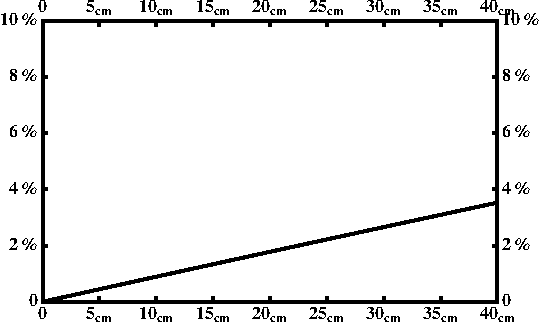
\includegraphics[width=\figwidth,height=\qfigheight]{\figures/intro/decays/Hydrogen_conversion_Prob_4Photons.pdf}
\caption[Probability of pair production, $\gamma \to$\epem, as a function of distance in liquid hydrogen]{\label{fig:conversion}{Probability of pair production, $\gamma \to$\epem, as a function of distance in liquid hydrogen.}}
\end{center}\end{figure}
This type of subprocess mimics the Dalitz decay \piz $\to e^+e^- \gamma$, described in Sec.~\ref{sec:dalitzdecay}. Since there are 2 photons with equal probability of conversion, the total probability is double that shown in Fig.~\ref{fig:conversion}.
%
%
%
\subsection{Dalitz Decay}\label{sec:dalitzdecay} 
When a pseudoscalar meson decays via a photon $\gamma$ and a dilepton ($l^{+}l^{-}$) pair, it is known as a Dalitz decay or a so-called single off-shell decay. The Dalitz decay is related to the two photon decay. However, in the Dalitz decay, one of the photons is off-shell ($\gamma^*$) and decays into a dilepton pair. Since the Dalitz decay is related to the two photon decay, the form factor of the Dalitz decay, for P($\pi^{0}$, $\eta$, $\eta'$), will be similar to the form factor of the two photon decay of P($\pi^{0}$, $\eta$, $\eta'$), except there will be an effective mass dependence for the Dalitz decay. Figure~\ref{fig:piz.dalitz} depicts the Feymann diagram of the Dalitz decay.

The amplitude for the decay $P_P \to \gamma^\star(p) \gamma(k) \to l^+(p_+)l^-(p_-) \gamma(k)$ is given by the following expression:
\begin{equation}\label{eq:piz.eeg.amp}
{\cal M}(P\to l^+(p_+,s_+)l^-(p_-,s_-) \gamma) = {M}_P(p^2,k^2=0) \varepsilon_{\mu\nu\rho\sigma} \frac{1}{q^2} e \bar u(p_-,s_-) \gamma^\mu v(p_+,s_-) q^\nu \epsilon^\rho k^\sigma.
\end{equation}
Comparing the amplitudes of Eq.~\ref{eq:piz.eeg.amp} and Eq.~\ref{eq:piz.gg.amp} it is seen that the polarization of the off-shell photon turned into the current $e \bar u(p_-,s_-) \gamma^\mu v(p_+,s_-)$ of the lepton pair. The parameters $s_\pm$ are the spin helicities of the outgoing leptons $l^\pm$ and as in  Eq.~\ref{eq:piz.gg}, $\epsilon$ is the polarization of the outgoing photon. 
%
\subsubsection{\emph{Squared Matrix Element}}


\begin{align}\label{eq:piz.eeg}
& \left|{\cal M}(P\to l^+(p_+,s_+)l^-(p_-,s_-) \gamma)\right|^2 = \nonumber \\ & \frac{e^2}{q^4} \left|M\right|^2  \varepsilon_{\mu\nu\rho\sigma}\varepsilon_{\mu^{\prime}\nu^{\prime}\rho^{\prime}\sigma^{\prime}}\bar u(p_-,s_-) \gamma^\mu v(p_+,s_+) \bar v(p_+,s_+) \gamma^{\mu^{\prime}}  u(p_-,s_-) q^\nu \epsilon^\rho k^\sigma q^{\nu^{\prime}} \epsilon^{\rho^{\prime}} k^{\sigma^{\prime}} .
%
\end{align}
using an equation found between equation 5.3 and 5.4 found in~\cite{peskin}
\begin{align}\label{eq:spin.sum}
& \sum\limits_{s_{-},s_{+}}^{} \bar{u}(p_{-},s_{-})\gamma^{\mu}\nu(p_{+},s_{+})\bar{\nu}(p_{+},s_{+})\gamma^{\mu^{\prime}}u(p_{-},s_{-}) = Tr\left[ (\slashed{p}_- +m)\gamma^{\mu} (\slashed{p}_+-m)\gamma^{\mu^{\prime}} \right]\nonumber \\& =2q^{2}\left[-(g_{\mu\mu^{\prime}}-\frac{p_{\mu}p_{\mu^{\prime}}}{q^{2}} ) - \frac{(p_{+} - p_{-})_{\mu}(p_{+} - p_{-})_{\mu^{\prime}}}{q^{2}}\right]
\end{align}
where the identity $q = p_+ + p_-$ was used.
Substituting Eq.~\ref{eq:spin.sum} into Eq.~\ref{eq:piz.eeg}
\begin{align} \label{eq:piz.eeg.midway1}
\left|{\cal M}\right|^{2} =\frac{2e^{2}\left|M_{P}\right|^{2}}{q^{2}}\varepsilon_{\mu\nu\rho\sigma}\varepsilon_{\mu^{\prime}\nu^{\prime}\rho^{\prime}\sigma^{\prime}}\left[-g^{\mu\mu^{\prime}} - \frac{(p_{+} - p_{-})^{\mu}(p_{+} - p_{-})^{\mu^{\prime}}}{q^{2}}\right](-g^{\nu\nu^{\prime}})q^{\rho}k^{\sigma}q^{\rho^{\prime}}k^{\sigma^{\prime}}
\end{align}
Substituting $k = P - q$ and $p_- = q - p_+$ into Eq.~\ref{eq:piz.eeg.midway1}
\begin{align} \label{eq:piz.eeg.midway2}
\left|{\cal M}\right|^{2} = & \frac{2e^{2}\left|M_{P}\right|^{2}}{q^{2}}\varepsilon_{\mu\nu\rho\sigma}\varepsilon_{\mu^{\prime}\nu^{\prime}\rho^{\prime}\sigma^{\prime}}\left[-g^{\mu\mu^{\prime}} - \frac{(2p_{+} - q)^{\mu}(2p_{+} - q)^{\mu^{\prime}}}{q^{2}}\right] \nonumber \\ & \times (-g^{\nu\nu^{\prime}})      
(q^{\rho}P^{\sigma} - q^{\rho}q^{\sigma}) (q^{\rho}P^{\sigma^{\prime}} - q^{\rho^{\prime}}q^{\sigma^{\prime}})
\end{align}
Applying properties of $-g^{\mu\mu^{\prime}}$ and $-g^{\nu\nu^{\prime}}$ onto Eq.~\ref{eq:piz.eeg.midway2}
\begin{align} \label{eq:piz.eeg.midway3}
\left|{\cal M}\right|^{2} = & \frac{2e^{2}\left|M_{P}\right|^{2}}{q^{2}}
\left[\varepsilon_{\mu\nu\rho\sigma}\varepsilon^{\mu\nu}_{\quad \rho^{\prime}\sigma^{\prime}}q^{\rho}P^{\sigma}q^{\rho^{\prime}}P^{\sigma^{\prime}} + \frac{4}{q^2} \varepsilon_{\mu\nu\rho\sigma}\varepsilon^{\mu}_{\ \ \nu^{\prime} \rho^{\prime}\sigma^{\prime}} p_{+}^{\nu}p_{+}^{\nu^{\prime}}q^{\rho}q^{\rho^{\prime}}P^{\sigma}P^{\sigma^{\prime}}\right]
\end{align}
Switching to the rest frame of the pseudoscalar meson, $P_p$, the 4-momenta is transformed to $P^\sigma = m_p\delta^{\sigma 0}$. The squared amplitude of Eq.~\ref{eq:piz.eeg.midway3} reads;
\begin{align} \label{eq:piz.eeg.midway4}
\left|{\cal M}\right|^{2} = & \frac{2e^{2}\left|M_{P}\right|^{2}}{q^{2}}m_p^2
\left[\varepsilon_{\mu\nu\rho}\varepsilon^{\mu\nu}_{\ \ \rho^{\prime}}q^{\rho}q^{\rho^{\prime}} - \frac{4}{q^2} \varepsilon_{\mu\nu\rho}\varepsilon^{\mu}_{\ \nu^{\prime}\rho^{\prime}} p_{+}^{\nu}p_{+}^{\nu^{\prime}}q^{\rho}q^{\rho^{\prime}}\right]
\end{align}
The sign change is due to $g^{\sigma \sigma^{\prime}} = -\delta^{\sigma \sigma^{\prime}}$. 
Using the antisymmetric tensor properties $\varepsilon_{\mu\nu\rho}\varepsilon^{\mu\nu}_{\ \ \rho^{\prime}} = 2\delta_{\rho\rho^{\prime}}$ and $\varepsilon_{\mu\nu\rho}\varepsilon^{\mu}_{\ \nu^{\prime}\rho^{\prime}} = \delta_{\nu\nu^{\prime}}\delta_{\rho\rho^{\prime}} - \delta_{\nu\rho^{\prime}}\delta_{\rho\nu^{\prime}} = (\hat{e}_{\nu} \times \hat{e}_{\rho}) \cdot (\hat{e}_{\nu^{\prime}} \times \hat{e}_{\rho^{\prime}})$, Eq.~\ref{eq:piz.eeg.midway4} is reduced to 
\begin{align} \label{eq:piz.eeg.final}
\left|{\cal M}\right|^{2} =  \frac{2e^{2}\left|M_{P}\right|^{2}}{q^{2}}m_p^2
\left[2\left|\bf{q}\right|^2 - \frac{4}{q^2} \left|\bf{q}\right|^2 \left|\bf{p_{+}}\right|^2 \sin^2(\theta_{p_{_+}q}) \right]
\end{align}

\subsubsection{\emph{Decay rate}}
The decay rate of a three-body decay is given in Equation 46.19 of~\cite{pdg2014} as
\begin{align}\label{eq:pdg.3body}
d\Gamma = \frac{1}{(2 \pi)^5} \frac{1}{16 m_p^2} \left|{\cal M}\right|^2 \left|\bf{p_1^*}\right| \left|\bf{p_3}\right|d\Omega_1^*d\Omega_3 dm_{12} \ ,
\end{align}
%
where ($\left|\bf{p_1^*}\right|,\Omega_1^*$) is the momentum of particle 1 in the rest frame of 1 and 2, and $\Omega_3$ is the angle of particle 3 in the rest frame of the decaying particle $m_p$~\cite{pdg2014}. Relating Eq.~\ref{eq:pdg.3body} to the variables in Eq.~\ref{eq:piz.eeg.final}, where $(\left|\bf{p_1^*}\right|,\Omega_1^*) = (\left|\bf{p_+}\right|,\Omega_{p_{_+}q})$, $m_{12} = q$ and $(\left|\bf{p_3}\right|,\Omega_3) = (\left|\bf{p_k}\right|,\Omega_k)$, reads;
\begin{align}\label{eq:pdg.3body.sub}
d\Gamma = \frac{1}{(2 \pi)^5} \frac{1}{16 m_p^2} \left|{\cal M}\right|^2 \left|\bf{p_+}\right| \left|\bf{p_k}\right|d\Omega_+d\Omega_k dq \ ,
\end{align}
%
In the rest from of the decaying particle $m_p$, the 3-momenta $\left|\bf{p_k}\right| = \left|\bf{q}\right|$ and the solid angle $\Omega_k = \Omega_q$. Substituting the square matrix element from Eq.~\ref{eq:piz.eeg.final} into Eq.~\ref{eq:pdg.3body.sub} yields;
%
\begin{align}\label{eq:pdg.3body.sub2}
d\Gamma = \frac{1}{(2 \pi)^5} \frac{1}{16 m_p^2} \frac{2e^{2}\left|M_{P}\right|^{2}}{q^{2}}m_p^2
\left[2\left|\bf{q}\right|^2 - \frac{4}{q^2} \left|\bf{q}\right|^2 \left|\bf{p_{+}}\right|^2 \sin^2(\theta_{p_{_+}q}) \right] \left|\bf{p_+}\right| \left|\bf{q}\right|d\Omega_{p_{_+}q}d\Omega_q dq\ .
\end{align}
The variables $\left|\bf{q}\right|$ and $\left|\bf{p_+}\right|$ can be redefined, by means of Eq.~46.20b and Eq.~46.20a of~\cite{pdg2014}, as 
\begin{align}
\left|\bf{q}\right| = \frac{m_p^2 - q^2}{2m_p} \label{eq:eeg.qeq} \\
\left|\bf{p_+}\right| = \frac{\sqrt{q^2 - 4m_l^2}}{2} = \frac{q\sqrt{1 - \frac{4m_l^2}{q^2} } } {2} =\frac{q {\cal K}  } {2}  \label{eq:eeg.p+eq} \ ,
\end{align} 
where ${\cal K} = \sqrt{1 - \frac{4m_l^2}{q^2}}$. Replacing the variables calculated in Eq.~\ref{eq:eeg.qeq} and Eq.~\ref{eq:eeg.p+eq} into Eq.~\ref{eq:pdg.3body.sub2} and collecting terms yields;
\begin{align}\label{eq:pdg.3body.sub3}
d\Gamma = \frac{1}{(2 \pi)^5} \frac{1}{16 m_p^2} \left|M_{P}\right|^{2} \left[ \frac{2e^2 m_p^2}{8} \left( \frac{m_p^2 - q^2}{2 m_p}\right)^3\right]\left( 2 -{\cal K}^2\sin^2(\theta_{p_{_+}q})\right)\frac{{\cal K}}{4 q^2}dq^2d\Omega_{p_{_+}q}d\Omega_q \ ,
\end{align}
where the identity $qdq = \frac{dq^2}{2}$. Performing the integration of $\Omega_{p_{_+}q}d\Omega_q$ and replacing $e^2 = 4\pi\alpha$ transforms Eq.~\ref{eq:pdg.3body.sub3} into;
\begin{align}\label{eq:pdg.3body.sub4}
d\Gamma = \frac{1}{(2 \pi)^3} \frac{1}{32} \frac{4 \pi \alpha}{3} \left|M_{P}\right|^{2} \left[ \frac{m_p^6 \left( 1- \frac{q^2}{m_p^2}\right)^3}{m_p^3} \right]\left( 3 -{\cal K}^2\right)\frac{{\cal K}}{q^2}dq^2\ ,
\end{align}
which can be simplified further to;
\begin{align}\label{eq:eeg.final}
d\Gamma = \left(\frac{1}{64\pi} \left|M_{P}\right|^{2}m_{P}^{3} \right) \frac{2 \alpha}{3 \pi} \frac{1}{q^2} \left( 1- \frac{q^2}{m_p^2}\right)^3 \left( 1+ \frac{2m_l^2}{q^2}\right) \left( 1- \frac{4m_l^2}{q^2}\right)^{\frac{1}{2}} dq^2\ .
\end{align}
%
The form factor ${M}_P(p^2,k^2=0)$ can be written as follows:
\begin{align}
 {M}_P \to {M}_P \times \left|F(q^2)\right| \ ,
\end{align}
where $M_p$ is the decay constant of two photons mentioned in Sec.~\ref{sec:piz.gg} and $\left|F(q^2)\right|$ is called the transition form factor, which defines the electromagnetic space structure of the meson. 

It can be seen that the first set of variables in parenthesis in Eq.~\ref{eq:eeg.final} is Eq.~\ref{eq:piz.gg.decay.final}, therefore;
\begin{align}\label{eq:eeg.final}
\frac{d\Gamma}{\Gamma_{\gamma\gamma} dq^2} = \frac{2 \alpha}{3 \pi} \frac{1}{q^2} \left( 1- \frac{q^2}{m_p^2}\right)^3 \left( 1+ \frac{2m_l^2}{q^2}\right) \left( 1- \frac{4m_l^2}{q^2}\right)^{\frac{1}{2}} \left|F(q^2)\right|^2 \ ,
\end{align}
which is the Kroll-Wada equation founded in~\cite{KrollWada}.

The value of $\left|F(q^2)\right|$ can be directly measured by comparison of the differential cross section with that of Q.E.D. pointlike differential cross section i.e.
\begin{align}
\frac{d\sigma}{dq^{2}} = \left[\frac{d\sigma}{dq^{2}}\right]_{\text{pointlike}}\left| F(q^{2})\right| ^{2}\nonumber \ ,
\end{align}
or by performing a line shape analysis on the $l^{+}l^{-}$ invariant system using assumptions on the structure of $\left|F(q^2)\right|$. One such assumption for $\left|F(q^2)\right|$ is the dipole approximation in which 
\begin{align}
F(q^{2}) = [1-\frac{q^{2}}{\Lambda^{2}}]^{-1} \nonumber
\end{align}
\subsection{Summary}
The two photon decay and the Dalitz decay have different branching ratios. This difference is attributed to the factor of $\alpha$ along with a $q^2$ dependence calculated in the Dalitz decay. However, due to the probability of a photon converting into an electron-positron pair in $\ell$H$_2$, the total amount of \epem pairs produced via photon conversion is about the same as via Dalitz decay.
 
%\subsection{Meson Spectroscopy}\label{sec:intro.spect}
Meson spectroscopy is a comprehensive subfield of particle physics that is dedicated to the study of the mass spectrum and the quantum numbers of mesons. Meson spectroscopy also studies mesons decay channels, decay widths, production mechanisms and other physical attributes. Meson spectroscopy's goal is to gain insight into \abbr{QCD} and its interactions though mentioned measurements forming a firmer experimental and theoretical grounds on known and unknown physics and phenomena.


\graphicspath{{/Users/Mike/phdthesis/MY_THESIS}}
\chapter{The CLAS detector at Thomas Jefferson National Accelerator Facility }\label{sec:clas}

The Thomas Jefferson National Accelerator Facility (\abbr{TJNAF}\label{abbr:tjnaf}, Fig.~\ref{fig:jlab.aerial}), also known as Jefferson Laboratory (\abbr{JLab}\label{abbr:jlab}) is located in Newport News, Virgina. It is one of 17 national laboratories funded by the U.S. Department of Energy and is home to three experimental halls, \desg{A}, \desg{B}, \desg{C}, and the Continuous Electron Beam Accelerator Facility,\cite{cebaf} (\abbr{CEBAF}\label{abbr:cebaf}, Fig.~\ref{fig:jlab.cebaf}).

\abbr{JLab}'s stated mission is ``to provide forefront scientific facilities, opportunities and leadership essential for discovering the fundamental structure of nuclear matter; to partner in industry to apply its advanced technology; and to serve the nation and its communities through education and public outreach."\cite{Jlabwiki} In addition to its science mission, the lab provides programs designed to help educate the next generation in science and technology, and to engage the public.
%\abbr{JLab} also conducts a variety of research using its Free-Electron Laser, which is based on the same electron-accelerating technology used in \abbr{CEBAF}.

The analysis performed in this work utilizes experimental data collected with the \abbr{CEBAF} Large Acceptance Spectrometer (\abbr{CLAS}) in hall \desg{B}, using \abbr{CEBAF}. The experiment \g12 collected over 126~TB of raw data in 44 days of beam time from April to June 2008, making \g12 the world's largest multi-particle dataset in the energy range 1.77 GeV $\mathrm{< \sqrt{s} <}$ 3.33 GeV. This chaper is dedicated to the explanation of \abbr{CEBAF}, \abbr{CLAS} and other subsystems used during the \g12 run period.


\begin{figure}[H]
%\begin{center}
\centering
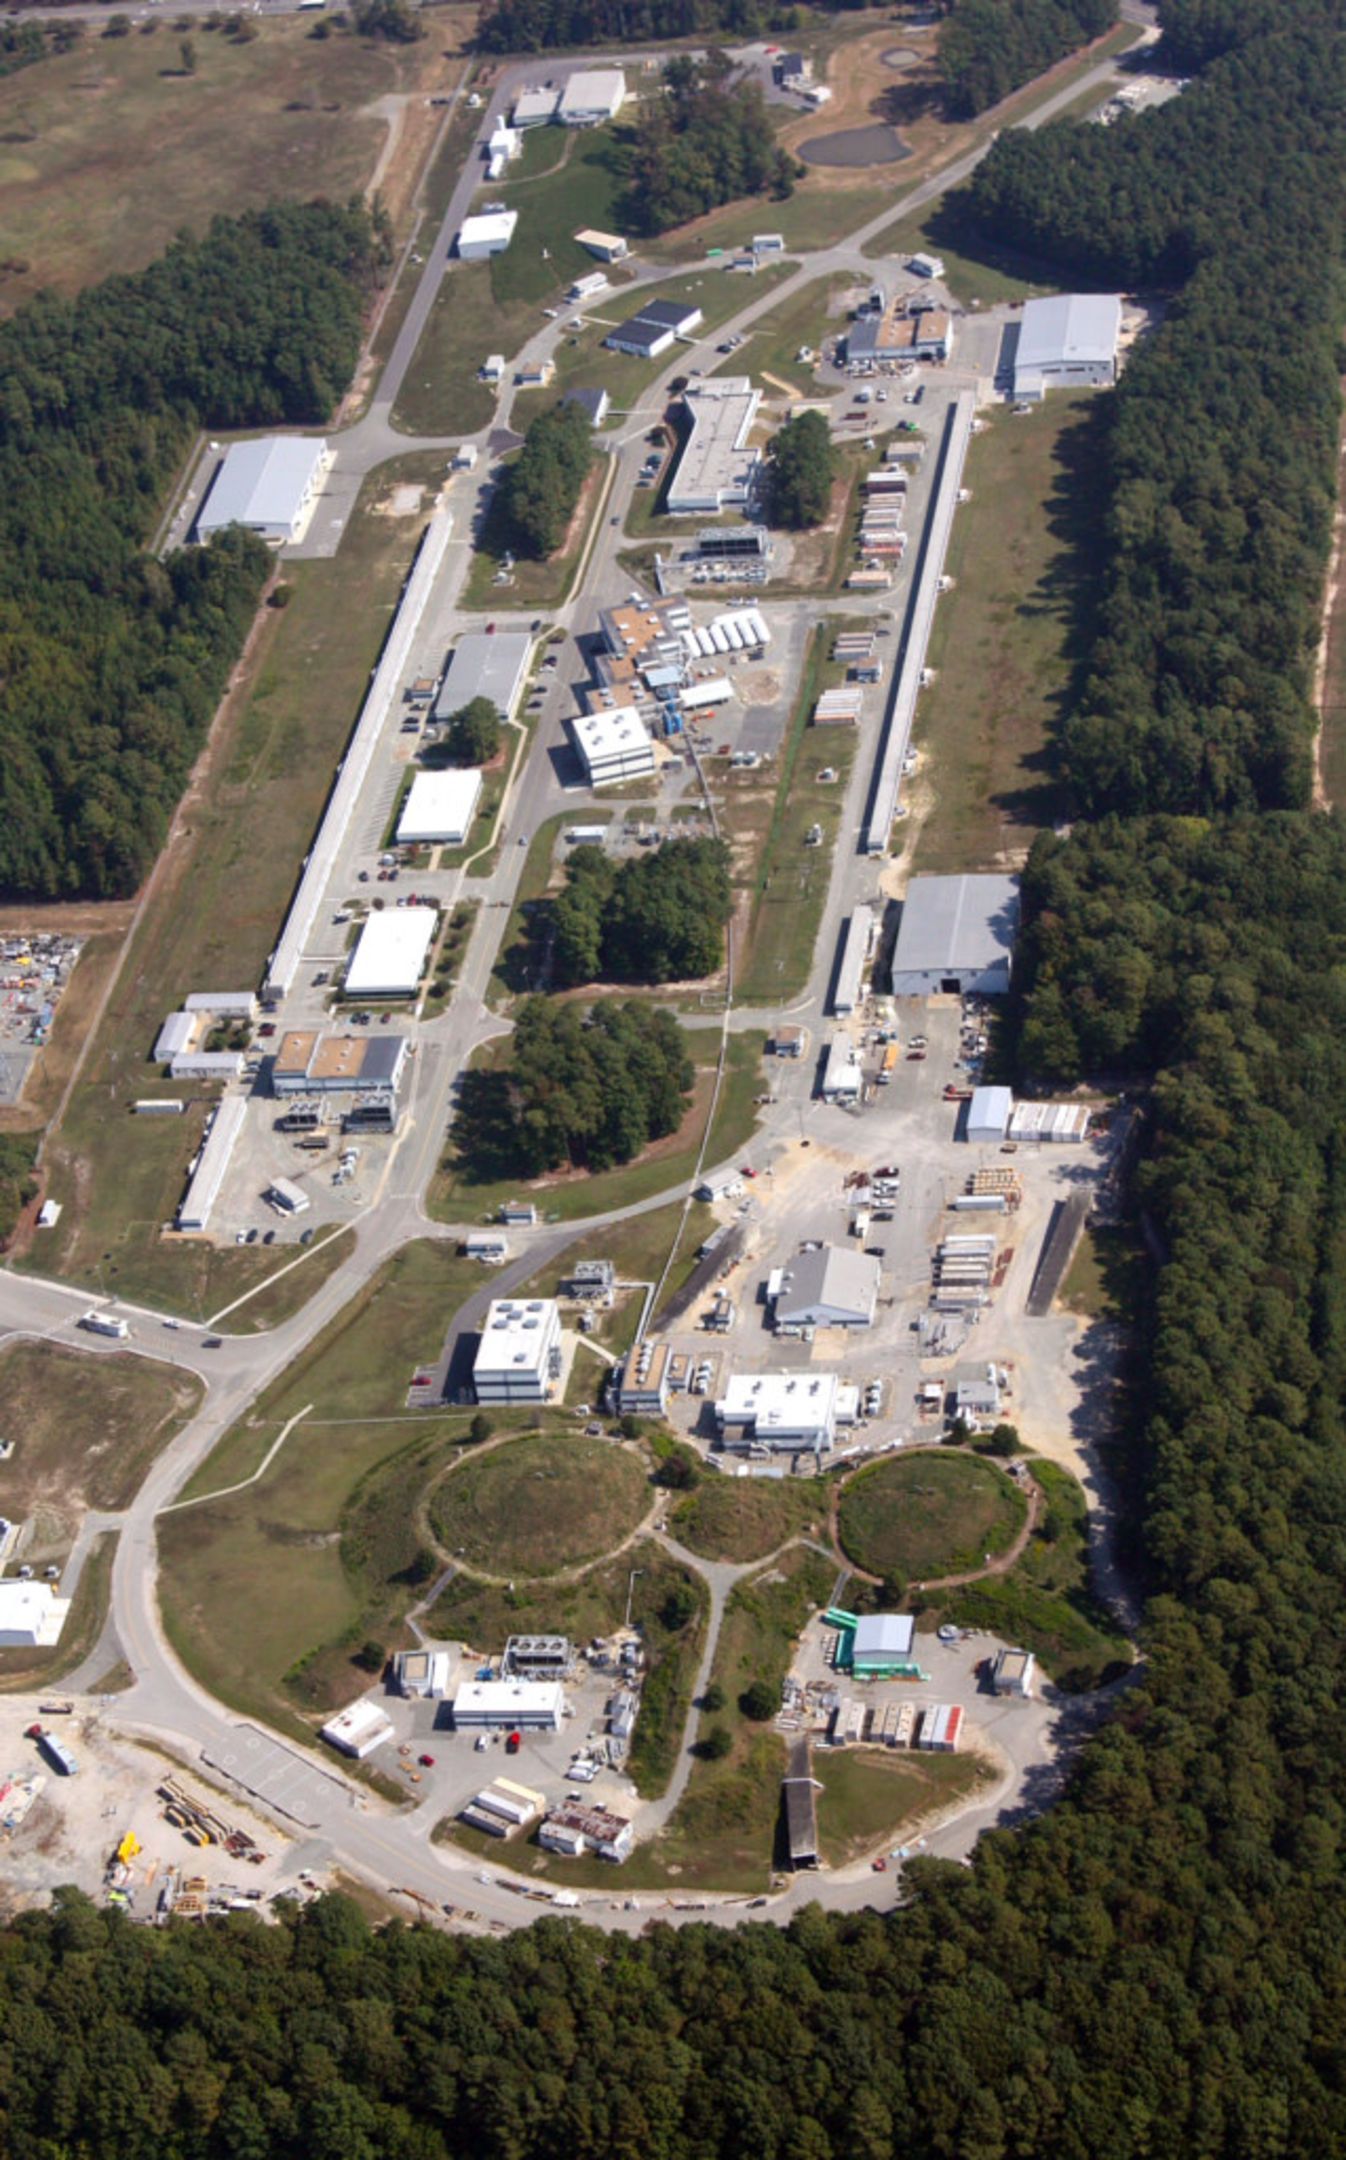
\includegraphics[width=0.6\columnwidth ,height=\hfigheight]{\grpath/jlab/jlab_arial_view_II.pdf}
\caption[Aerial view of Jefferson Laboratory (\abbr{JLab}) facing east]{\label{fig:jlab.aerial}Aerial view of Jefferson Laboratory (\abbr{JLab}) facing east. Image Source: \cite{cebafflckr}}
%\end{center}
\end{figure}
%
\begin{figure}\begin{center}
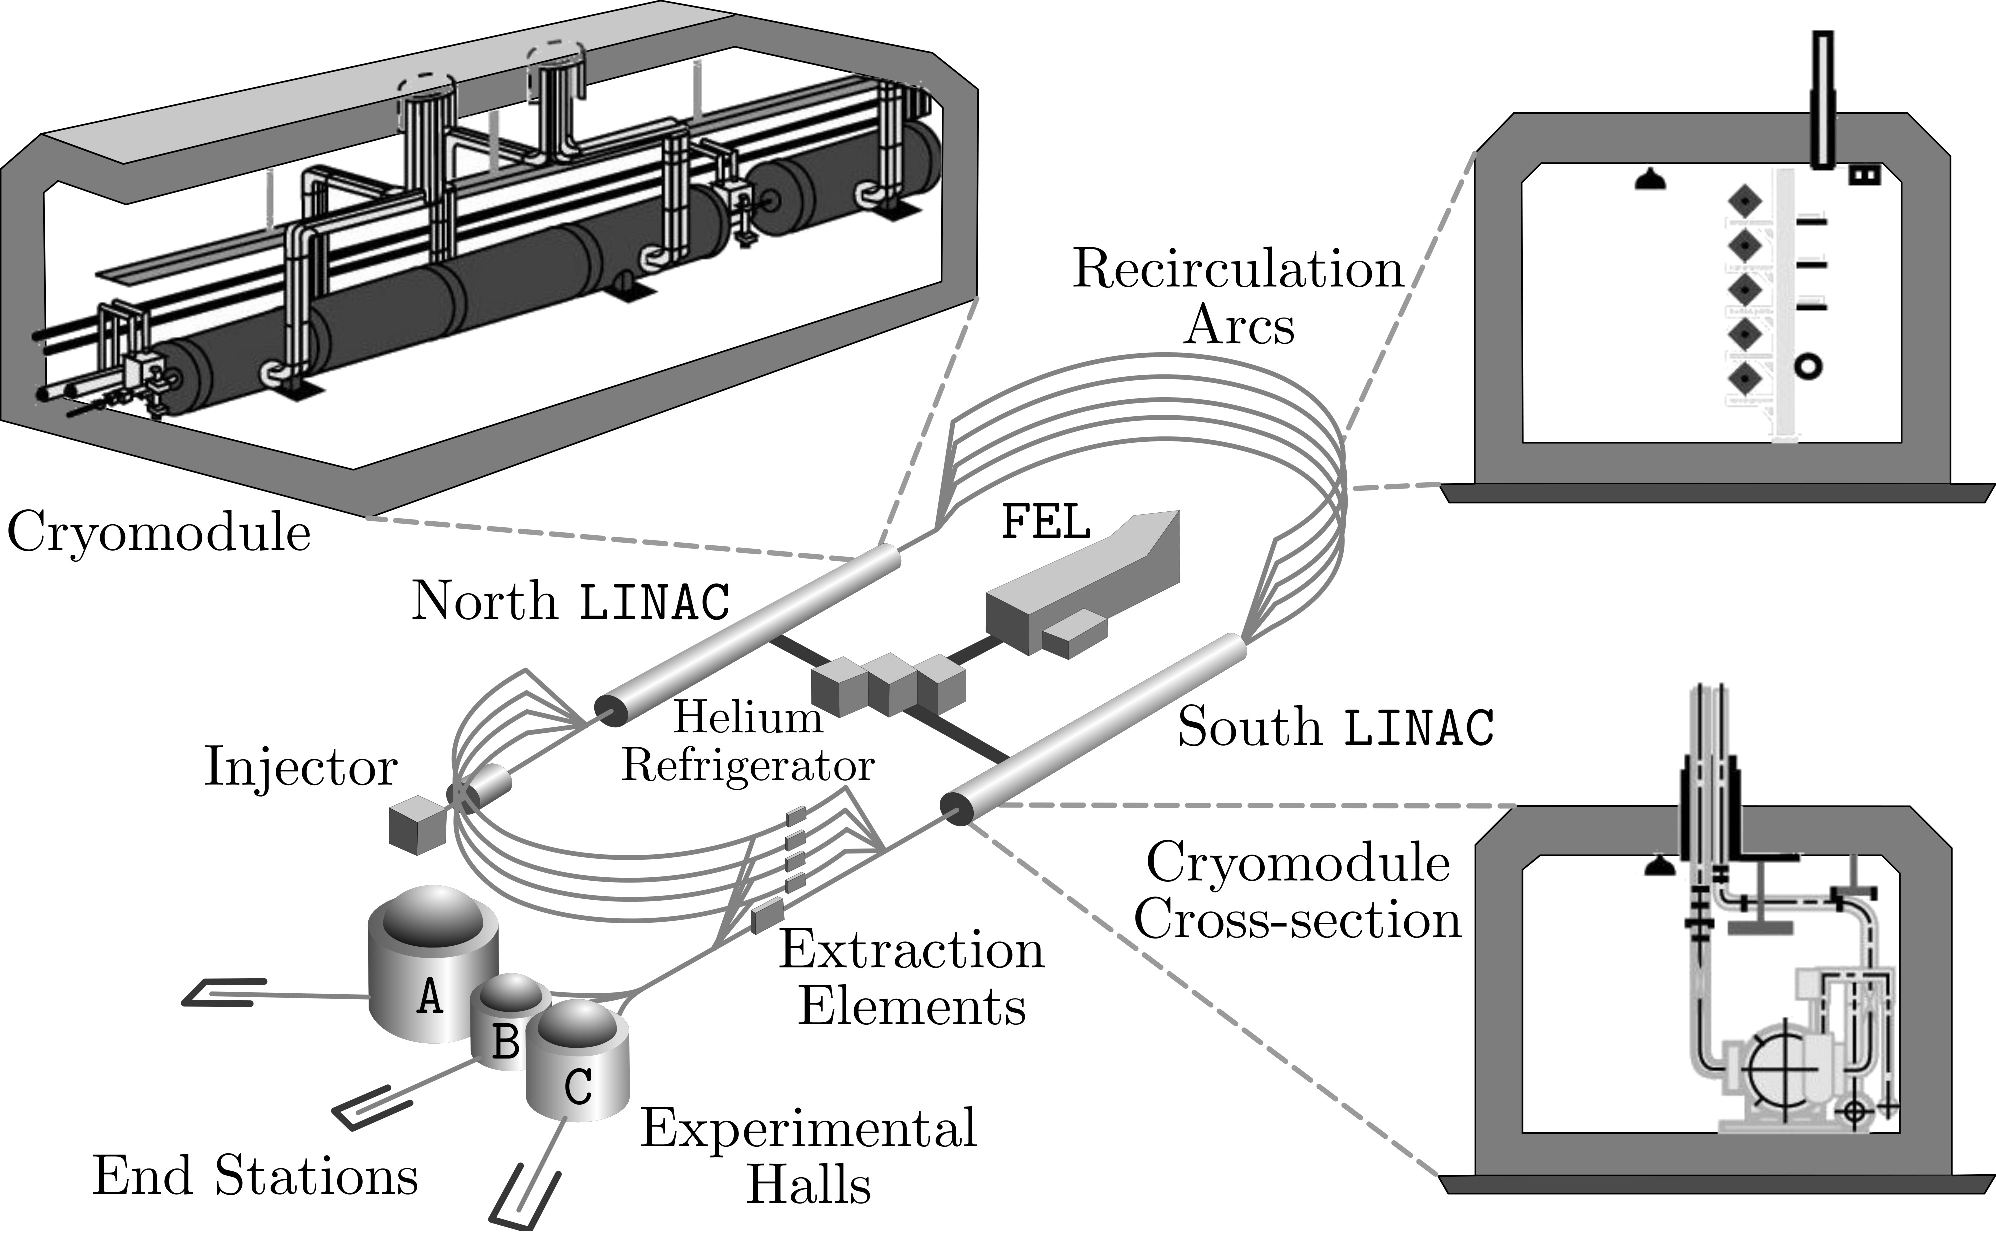
\includegraphics[width=0.9\columnwidth, height=\qfigheight]{\grpath/jlab/cebaf.pdf}
\caption[The Continuous Electron Beam Accelerator Facility (\abbr{CEBAF}) at Jefferson Laboratory (\abbr{JLab})]{\label{fig:jlab.cebaf}The Continuous Electron Beam Accelerator Facility (\abbr{CEBAF}) at Jefferson Laboratory (\abbr{JLab}) showing cross-sections of the linear accelerator (\abbr{LINAC}) halls and the recirculation arcs. Also depicted are the Free Electron Laser (\abbr{FEL}\label{abbr:fel}) and the helium refrigerator and distribution facility. Image Source:\cite{cebaf}}
\end{center}\end{figure}
\FloatBarrier
\section{Continuous Electron Beam Accelerator Facility}\label{sec:cebaf.desc}

\abbr{CEBAF} utilizes superconducting radio-frequency (\abbr{srf}\label{abbr:srf}) cavities to accelerate electrons and provide a continuous wave beam with 75\% polarization to the three halls simultaneously. A list of some specifications for \abbr{CEBAF} can be found in Table~\ref{tab:cebafspecs}.
%Niobium (\abbrlc{N}{b}\label{abbr:nb}), in a cryogenic system, provides the superconducting environment necessary for \abbr{CEBAF} to obtain a 100\% duty factor because superconducting cavities are non-resistive. Prior to the implementation of \abbr{srf}, copper \abbr{RF}\label{abbr:rf} cavities were used, however due to the resistive properties of copper significant cooling time was needed due to heat produced in the cavity.
\begin{table}
\begin{minipage}{\textwidth}
\begin{center}
\begin{singlespacing}

\caption[\abbr{CEBAF} Operating Specifications]{\label{tab:cebafspecs}Operating specifications of \abbr{CEBAF} at \abbr{JLab}.\cite{cebaf}}

\begin{tabular}{c|c}

%\hline \hline
%
%operation & \multicolumn{3}{c}{Generation} \\
%charge & I & II & III \\


\hline

$\textrm{E}_{min}$ & 0.6 GeV \\
$\textrm{E}_{max}$ & 6.0 GeV \\
$\textrm{I}_{max}$ & 200 $\mu$A \\
Polarization & $\textgreater$ 75\% \\
Geometric emittance & $\textless \ 10^{9}$ m rad \\
Momentum Spread & $10^{-5}$ \\
Average currents (Halls A and C) & 1-150$\mu$A \\
Average currents (Hall B) & 1-100nA \\
Bunch charge & $\textless$ pC \\
Repetition rat & 499 MHz/hall \\ 
Beam size (rms transverse) & $\sim$ 80 $\mu$m \\
Bunch length (rms) & 300 fs, 90 $\mu$m \\
Energy spread & 2.5 x 10$^5$ \\
Beam power & $\textless$ \ MW  \\
Beam loss & $\textless \mu$A  \\
Number of passes & 5 \\
Number of accelerating cavities & 338 \\
Fundamental mode frequency & 1947 MHz \\
Accelerating cavity effective length & 0.5m \\
Cells/cavity  & 5\\
Average $Q_{0}$  & 4.0 x 10$^9$ \\
Implemented $Q_{ext}$  & 5.6 x 10$^6$ \\
Cavity impedance (r/Q)  & 980 $\Omega$ \\
Average cavity accelerating gradient  & 7.5 MV/m \\
RF power  & $\textless$ \ 3.5 kW/cavity \\
Amplitude control  & 1.00 x 10$^{-4}$ rms \\
Phase control  & 0.1$^\circ$ rms \\
Cavity operating temperature  &  2.08 K\\
Heat load @ 2 K  &  $\textless$ 9 W/cavity\\
Liquefier 2 k cooling power  & 5kW \\
Liquefier operating power  &  5MW\\




\hline \hline

\end{tabular}

\end{singlespacing}
\end{center}
\end{minipage}
\end{table}
\vspace{20pt} 

To achieve the running conditions described in Table~\ref{tab:cebafspecs} \abbr{CEBAF} uses a GaAs photocathode laser driven injector system to produce a highly polarized electron beam. The laser pulses create three electron bunches that are bunched together in 2 ns groups, about 90 $\mu$m in length. Each bunch is 499~MHz at the source at 100 keV, spaced apart by 120$^\circ$ of \abbr{rf} phase. Together the electron bunches form a 1497 MHz beam that then enters two 1/4 \abbr{srf} cavities which accelerate the electrons to $\sim$1\% of the total machine energy before it is injected into the \abbr{CEBAF}'s main accelerator. 

When the electron bunches enter the \abbrlc{N}{b} \abbr{srf} cavity, they undergo an acceleration gradient provided by \abbr{rf} standing wave established inside of the cavity. The standing waves are kept in phase with the electron bunches resulting in a continuous positive electric force on each bunch as it passed through a cavity, see Fig.~\ref{fig:jlab.accel}

\begin{figure}\begin{center}
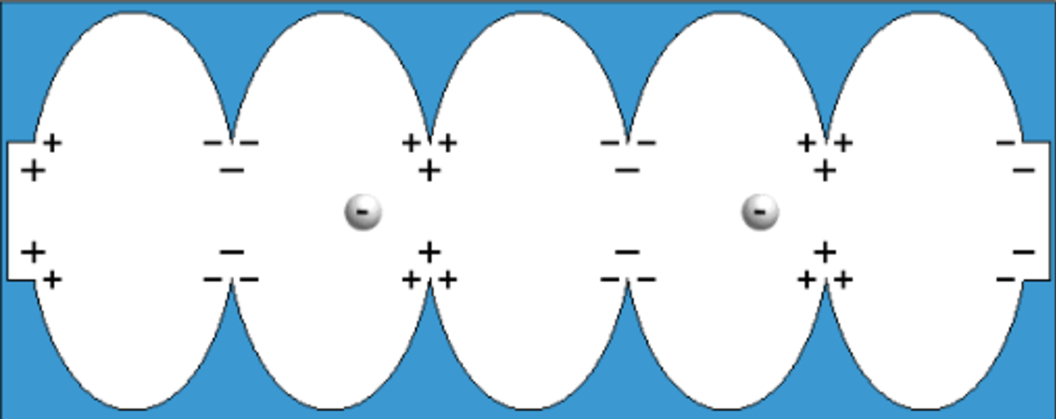
\includegraphics[width=0.8\figwidth,height=\qfigheight]{\grpath/jlab/accelerating_diagram.pdf}
\caption[Accelerating Cavity Diagram]{\label{fig:jlab.accel}Accelerating Cavity Diagram. Electron clusters experience a continuous acceleration due to a standing electromagnetic wave indicated by the positive and negative signs along the inner wall.}
\end{center}\end{figure}

The main accelerator, Fig.~\ref{fig:jlab.cebaf}, consists of a pair of linear accelerators (\abbr{LINAC}s\label{abbr:linac}). Each \abbr{LINAC} contains 168 \abbr{srf} \abbrlc{N}{b} cavities that are submerged in liquid Helium and cooled to 2.08 K, the temperature by which \abbrlc{N}{b} becomes superconducting. In total there are twenty cryogenic modules, each containing eight superconducting niobium cavities as depicted. in Fig.~\ref{fig:jlab.cavity}. 
%The significant cooling requirements are satisfied by the Lab's Central Helium Liquefier (\abbr{CHL}\label{abbr:chl}). 


\begin{figure}\begin{center} 
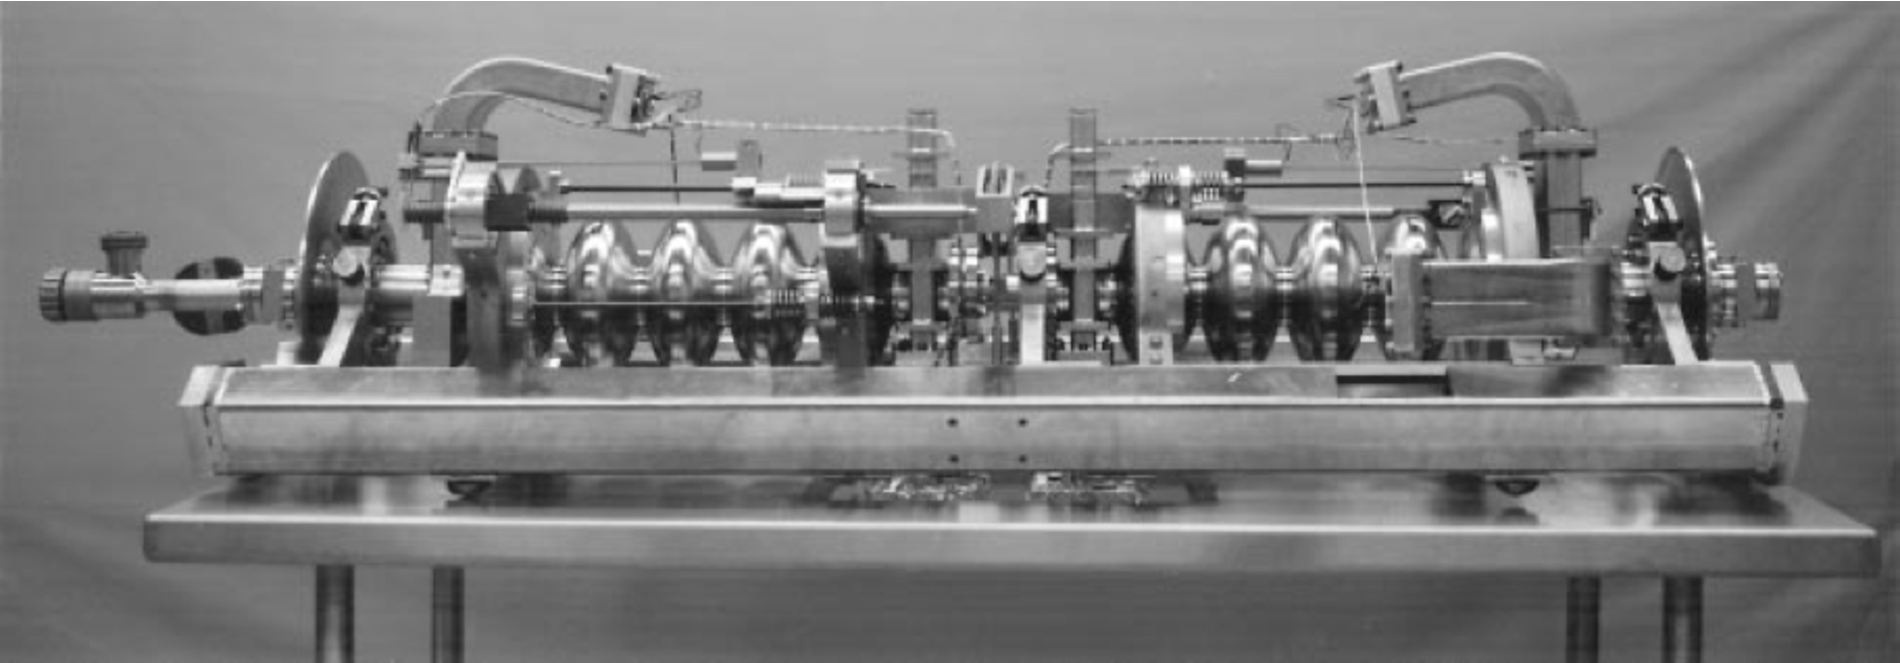
\includegraphics[width=\figwidth, height=\qfigheight]{\grpath/jlab/niobium_cavity_pair.pdf}
\caption[A \abbr{CEBAF} superconducting niobium cavity pair]{\label{fig:jlab.cavity}A \abbr{CEBAF} superconducting niobium cavity pair. Image Source: \cite{cebaf}}
\end{center}\end{figure}

The beam, once inside the \abbr{LINAC} can be passed up to five times. The \abbr{LINAC}s are connected by two sets of 180$^\circ$ magnetic-dipole bending arcs (see Fig.~\ref{fig:jlab.cebaf}) with a radius of 80~meters. The beam is sent through both accelerators and is then recirculated up to four more times. Each \abbr{LINAC} is capable of accelerating the beam by up to 600~MeV giving approximately 1.2~GeV per pass. Each hall can choose to extract the beam after any number of passes, however the fifth (final) pass can be sent to all three halls simultaneously. It should be noted that although each hall can receive the fifth pass, no two halls can run with the same lower energy \cite{clas.pass}. At the time of the \g12 experiment, the accelerator was capable of delivering a maximum electron beam energy of 5.714~GeV.
%\FloatBarrier
%\FloatBarrier
\section{Circular Polization} \label{sec:clas.polar}

As mentioned in Sec.~\ref{sec:cebaf.desc}, the electron beam provided by \abbr{CEBAF} has the capability of having 75\% longitudinal polarization. Longitudinal polarized electrons produce circularly polarized photons in the bremsstrahlung process on any target, however intensity of photon beam depends on Z of target. The circular polarization production process is quantum mechanical. From QED calculations, the degree of circular polarization transfer to the photon, $P_{circ}$, is seen to depend on the ratio of the relative electron energy to the bremsstrahlung photon, $\epsilon$:
%The experiment \g12 used a Au foil as a radiator therefore \g12 had a circular polarized beam.
\begin{equation}\label{eq:polarization}
	P_{circ} = (\frac{4\epsilon - \epsilon^{2}}{4-4\epsilon+3\epsilon^{2}})P_{e} \cite{Olsen}
\end{equation}
where $\epsilon = k/E_{0}$, $k$ is the bremsstrahlung photon energy and $E_{0}$ is the incident electron energy. Equation~\ref{eq:polarization} shows that circular polarization of the photon is transferred directly from the polarization of the electron, it also shows that the atomic nucleus or radiator plays no role in transfer of polarization. The transfer of circular polarization is maximum at the higher end of the energy spectrum $\epsilon$ and decreases towards the lower end of the spectrum as seen in Fig.~\ref{fig:jlab.polarization}. Figure~\ref{fig:jlab.polarization} also illustrates that polarization transfer is favored when the radiated photons take up large fractions of the incident electron energy. Coulomb and screening corrections (due to the atomic electrons) do not significantly affect the polarization of the emitted photons. 

\begin{figure}[h!]\begin{center}
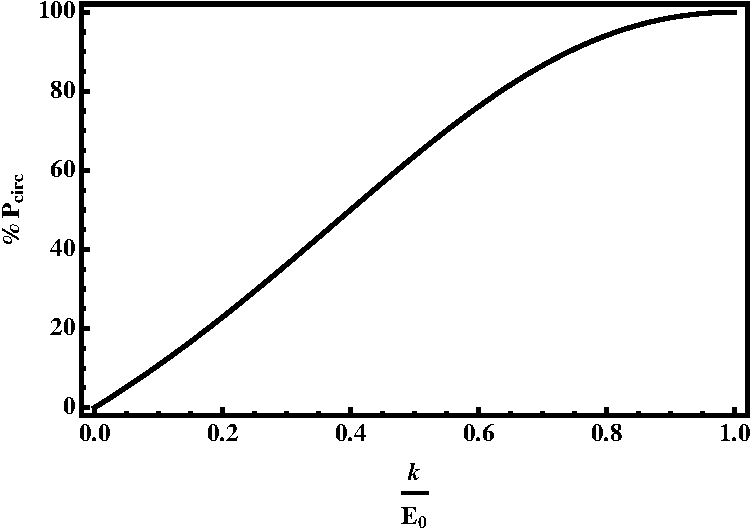
\includegraphics[width=0.8\figwidth,height=\qfigheight]{\grpath/hall-b/polarization.pdf}
\caption[Circular polarization Graph]{\label{fig:jlab.polarization}QED calculation for the degree of circular polarization of 50-MeV electrons in lead. The curve shown is a Born-approximated calculation which neglects screening corrections. An exact calculation involving Coulomb and screening corrections (not shown) yields similar results.\cite{Olsen}}
\end{center}\end{figure}

\FloatBarrier
\section{Beam Positioning}\label{sec:clas.beam}
%\FloatBarrier
There are several beam monitoring stations in Hall \desg{B} before and after the \abbr{CLAS} detector (Fig.~\ref{fig:clas.beam.beforemonitors}) to scan the important details of the electron beam prior to conversion into a photon beam and the details of the photon beam before and after entering the target. Such quantities for the electron beam include position, intensity, dispersion, and current, and for the photon beam include position, dispersion and flux. Most of these monitoring stations are used by the accelerator group.
% to steer the beam to the target as they control all magnets that can substantially move the beam.
\begin{figure}[h!]\begin{center}
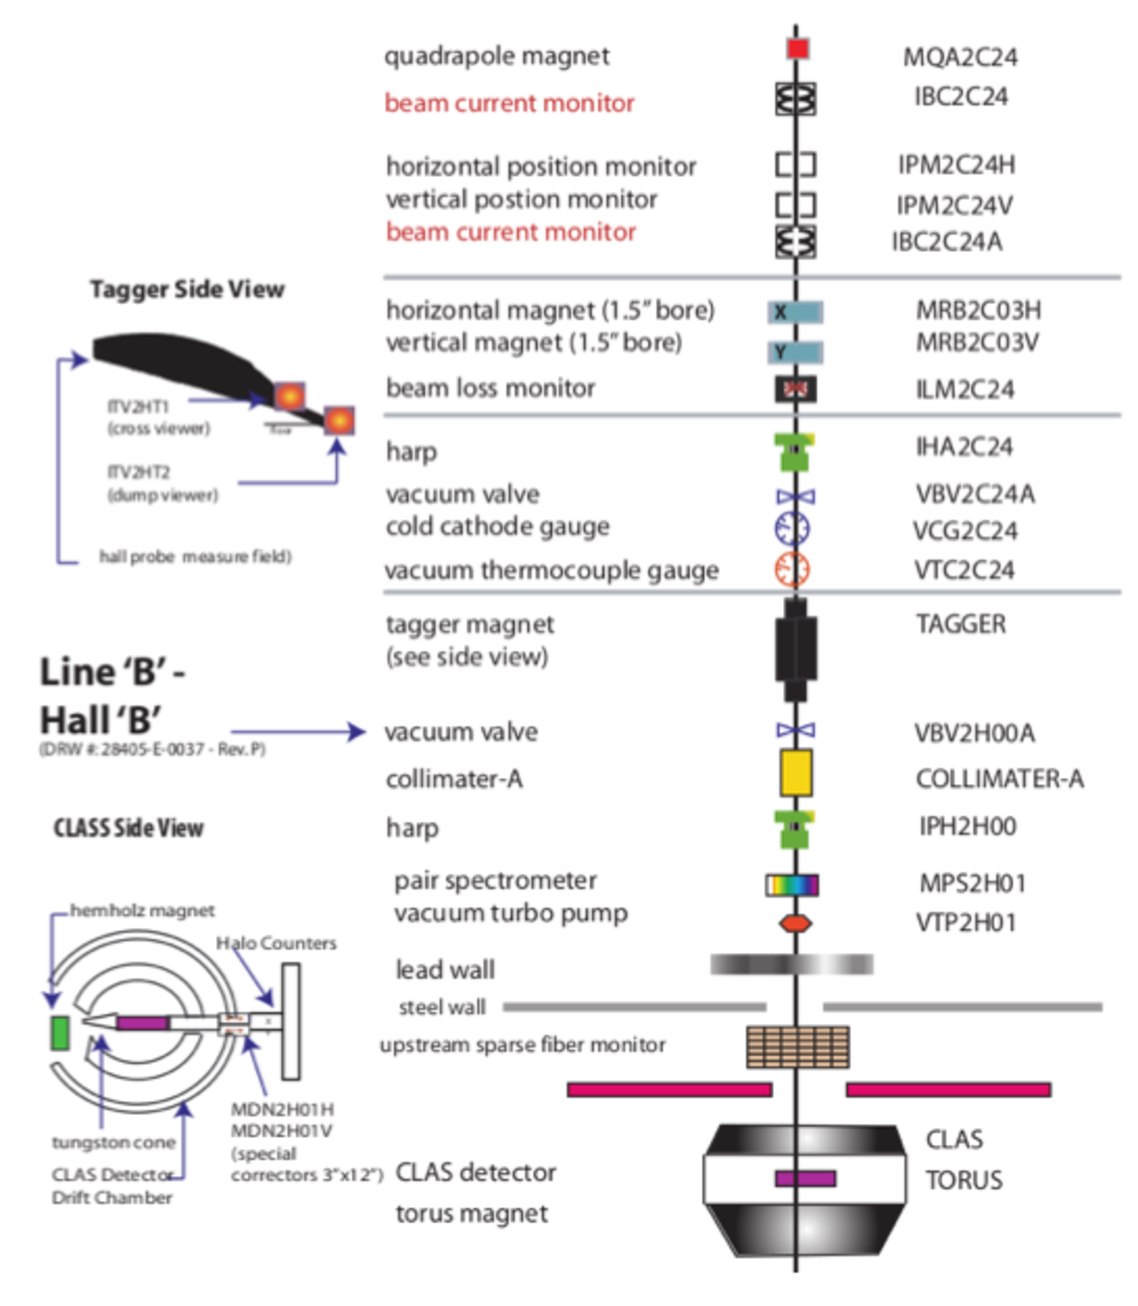
\includegraphics[width=\figwidth, height=1.75\hfigheight]{\grpath/hall-b/beamline_components.pdf}
\caption[Beamline and components of \abbr{CLAS}]{\label{fig:clas.beam.beforemonitors}{\coloronline}Beamline and components of \abbr{CLAS}. Image Source~\cite{cebafflckr}}
\end{center}\end{figure}
There are two types of devices to measure the electron beam position. The first type is represented by two beam position monitors (\abbr{BPM}s\label{abbr:bpm}) placed before the tagger. The position monitors use three radiofrequency cavities to measure the transverse location of the electron beam and its intensity. This information is used as feedback for the steering mechanism. The position monitors are noninvasive and measure at a rate of 1 Hz. 
The second type of device used to measure the beam position is the Harp Beam Profile Monitor, which also measures the electron beam dispersion. The harp devices consist of fine wires (20 and 50~{\um} W and 100~{\um} Fe) that can be passed through the beam at specific orientations and collect scattered electrons with a photomultiplier tube. This procedure measures the horizontal ($x$) and vertical ($y$) profile of the electron beam and is performed after any downtime or change in the beam. The accelerator group adjusts the beam position such that more than 99\% of the electron beam goes through the radiator. Since this process is invasive, it was only done when the drift-chambers and \abbr{DAQ} were turned off. A harp scan measurement for \g12 is shown in Fig.~\ref{fig:clas.beam.harpscan}. The width of the beam was contained within a 200 $\mathrm{\mu}$m diameter.



%\begin{figure}\begin{center}
%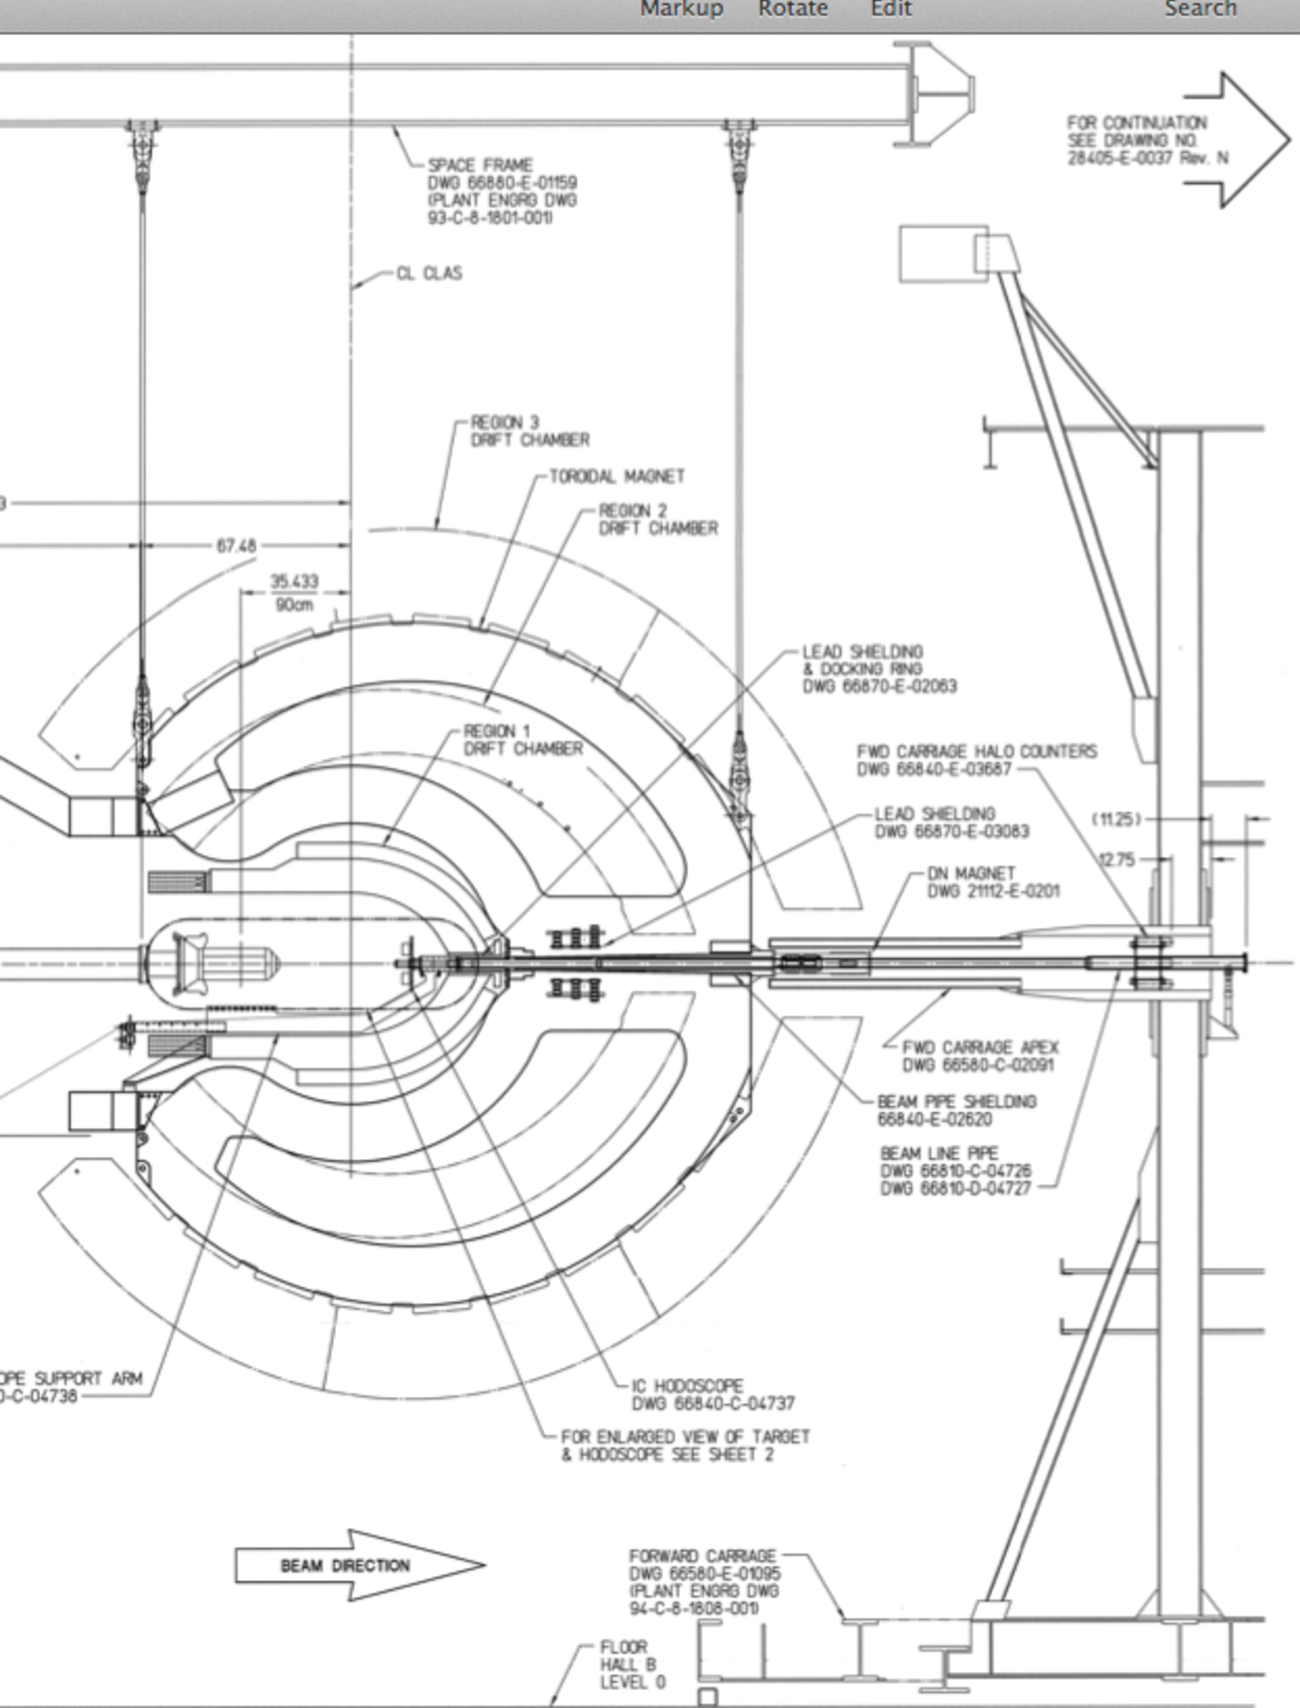
\includegraphics[width=\figwidth,height=\hfigheight]{\grpath/hall-b/G12_afterbeam_blueprint.pdf}
%\caption[Beamline and \abbr{CLAS} components in \g12]{\label{fig:clas.beam.aftermonitors}{\coloronline}Beamline and \abbr{CLAS} components in \g12}
%\end{center}\end{figure}

\begin{figure}\begin{center}
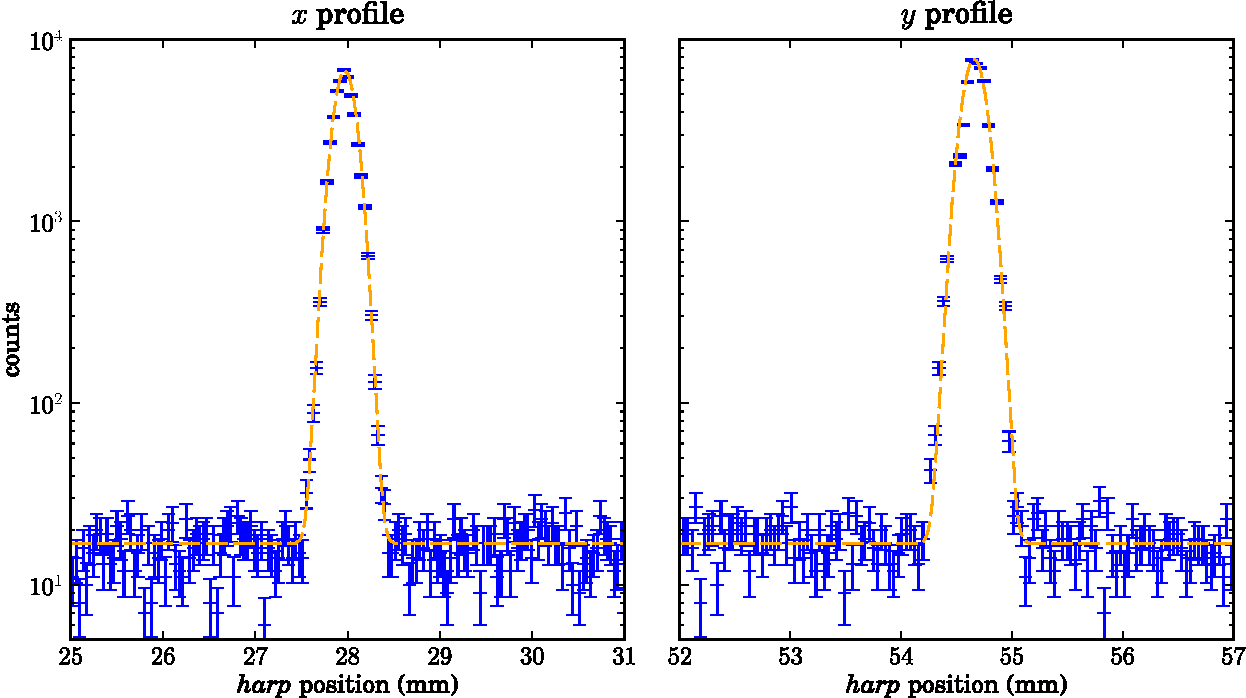
\includegraphics[width=\figwidth,height=\qfigheight]{\grpath/calibration/harpscan.pdf}
\caption[A typical \emph{harp} scan done just prior to run 56426]{\label{fig:clas.beam.harpscan}{\coloronline}A typical \emph{harp} scan done just prior to run 56426. Shown are the $x$ and $y$ profiles of the electron beam just before the tagger. The dashed orange line is a Gaussian fit to the data: $\sigma_x~=~0.115$~mm and $\sigma_y~=~0.105$~mm. Image Source:~\cite{goetz}}
\end{center}\end{figure}

The Total Absorption Shower Counter located downstream of \abbr{CLAS}, measures the photon flux (see Fig.~\ref{fig:clas.beam.afterCLAS}). The \abbr{TASC}, consists of four lead glass blocks of $\sim$ 17 radiation lengths, each coupled to a photo-multiplier tube (\abbr{PMT}\label{abbr:pmt}). The \abbr{TASC} is approximately 100\% efficient at detecting photons at beam currents less than 100~pA\cite{clas.tagger,clas.tagger.calib}. Since \g12 ran with 65~nA current, special low current, 50~pA, normalization runs(see Table~\ref{tab:data.calibruns}) were taken several times throughout \g12. The ratio of electrons detected in the photon tagger (see Sec.~\ref{sec:clas.tagr}) to that of photons detected in the \abbr{TASC} gives the tagging ratio used to calibrate the tagger and measure the flux throughout the entire \g12 run period.
%with hits in the left and right \abbr{TDC} matching in time and a corresponding hit in an E-counter
\begin{figure}[h!]\begin{center}
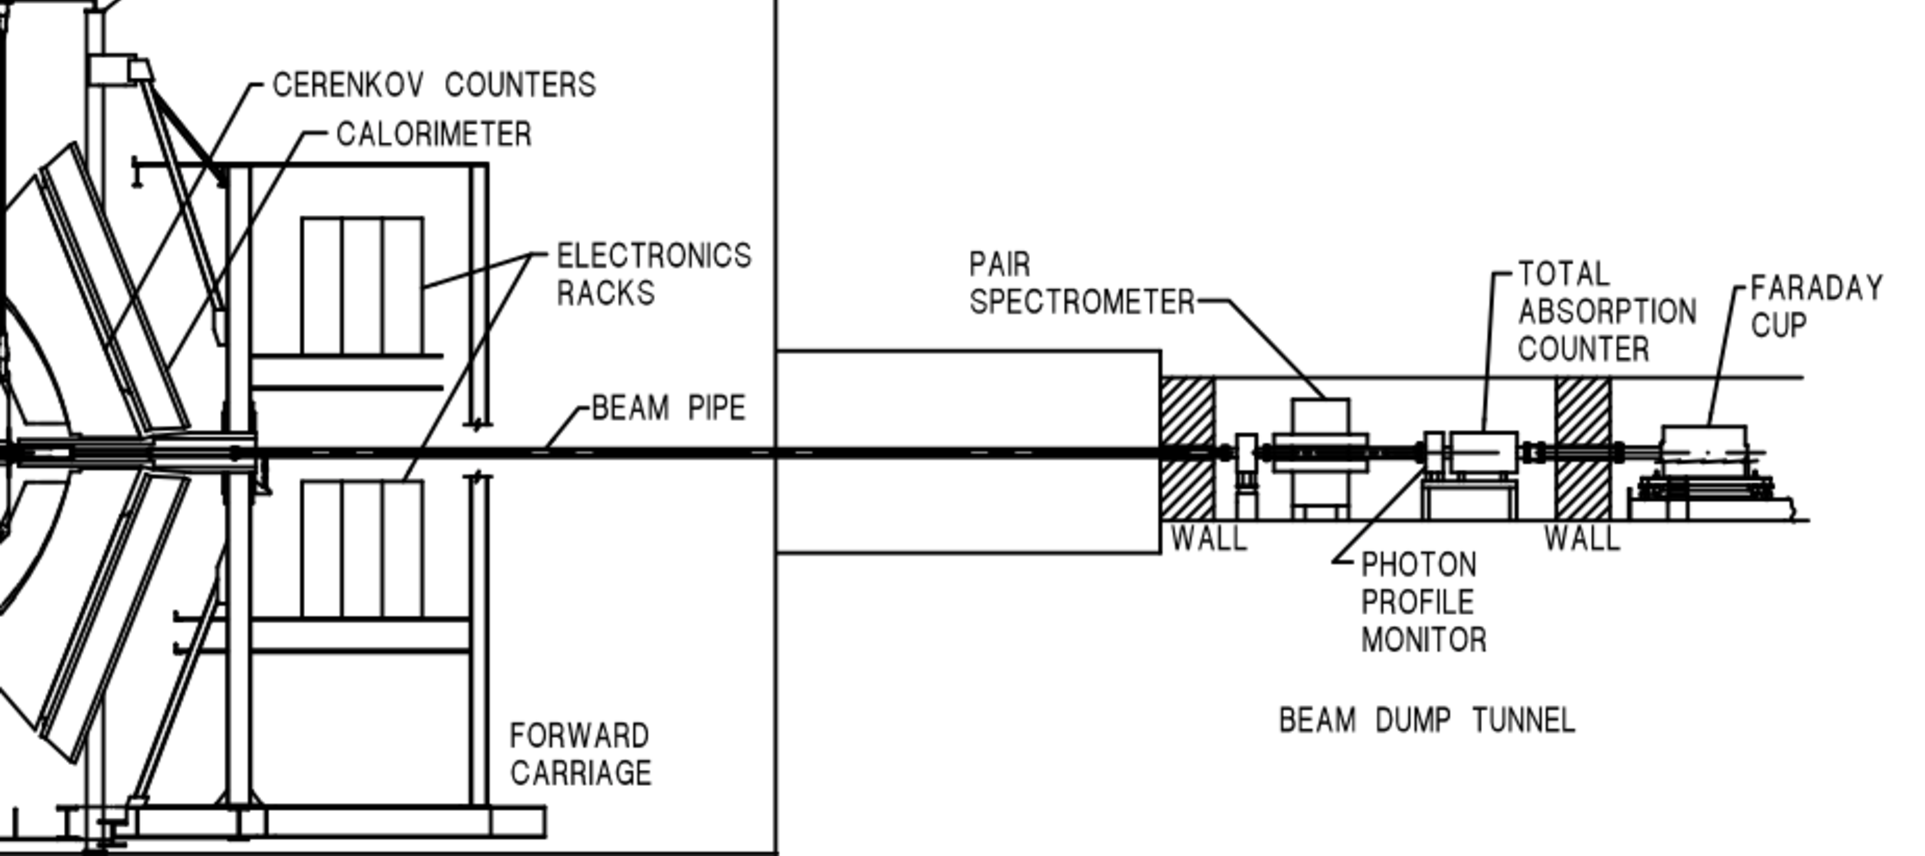
\includegraphics[width=\figwidth,height=0.8\qfigheight]{\grpath/hall-b/TASC_blueprint.pdf}
\caption[Beamline and components after \abbr{CLAS} ]{\label{fig:clas.beam.afterCLAS}{\coloronline}Beamline components in \g12 after \abbr{CLAS}}
\end{center}\end{figure}

\FloatBarrier
\section{Photon Tagger} \label{sec:clas.tagr}

The electron beam delivered to hall \desg{B} from \abbr{CEBAF} can be sent directly to a target or the electron beam can produce a \emph{real photon} beam by means of bremsstrahlung radiation by passing the electron beam through a radiator. Typical radiators have high atomic number to help reduce contamination of photons produced by electron-electron scattering. The \g12 experiment used a gold (\abbrlc{A}{u}) foil of $10^{-4}$~radiation length. This choice has a double purpose, to maximize the probability of the electron-nucleus interaction given that the bremsstrahlung cross section is proportional to $\mathrm{Z^{2}}$, and to minimize the number of interaction centers such that each electron interacts once, producing only one photon. After the electron beam passes through the radiator, the beam becomes a mixture of photons and electrons that did not interact with the radiator and recoil electrons. The mixed beam then travels into a dipole magnetic field which sweeps the electrons out of the electron-photon beam. The electrons present in the electron-photon beam are directed toward two hodoscope planes, each made of an overlapping array of scintillators to detect the energy-degraded electrons.

%  

The first scintillator plane, referred to as the E-plane (Figs.~\ref{fig:jlab.tagr.energies}, and~\ref{fig:jlab.tagr.paddles}), is used to determine the momentum of the recoiling electrons. The E-plane provides photon energy resolution on the order of 0.1\% of the incident electron beam energy. It consists of 384 paddles that are 20 cm long, 4 mm thick and from 6 to 18 mm wide. The paddles are arranged in an overlapping fashion, thus increasing the number of logical paddles to 767.
The trajectory of an electron or any charged particle in the magnetic field is governed by the equation
\begin{equation}\label{eq:motioninmag}
	p = qrB \ (\mathrm{if}\ \vec{p} \perp \vec{B} )
\end{equation}
where $p$ is the particle's momentum, $q$ is the particle's charge, $r$ is the particle's radius of curvature and $B$ is the magnetic field the particle passes through.
By determining which paddle an electron hit we know the radius of curvature and we can calculate the momentum of the electron. The momentum of the electron can then be used to obtain the energy of the photon by means of the conservation relation 
\begin{equation}\label{eq:tagger.energy}
	E_{\gamma} = E_{0} - E_{e}
\end{equation}
where $E_{0}$ is the energy of the incident electron given by \abbr{CEBAF}, $E_{e}$ is the energy of the recoil electron and $E_{\gamma}$ is the energy of the emitted photon. 

The second scintillator plane, referred to as the T-plane, is used to make accurate timing measurements of the recoiling electrons. This plane comprises of 61 paddles that are each 2 cm thick. The added thickness of these paddles allow for a timing resolution of 110 ps.
% The spectrometer was able to tag photons ranging from 20-95\% of the incident electron beam energy.

The tagger can tag photons of energies from 20 to 95\% of the incident electron beam energy. For \g12 this corresponds to a photon energy range of 1.142 - 5.425~GeV. Due to the high current of the electron beam delivered to \g12 from \abbr{CEBAF} there were usually more than one ``hit'' in the tagger for each event. Normally, the one associated with the photon that caused the event could be obtained by a timing coincidence with the tracks, although there are cases when this photon is ambiguous as discussed in Sec.~\ref{sec:analysis.beam}.

The photons that pass through the radiator then pass through a 6.2~mm diameter collimator. Collimation is used to trim the beam halo prior to arriving at the CLAS cryotarget. In the \g12 experiment the beam entering the cryotraget was 1.5~cm in radius. The collimator was positioned 537~cm upstream of the cryotarget which had a radius of 2~cm. A sweeping magnet were placed after the collimator to remove any charged particles created by interactions of photons with the collimator.

More detailed information on the Hall B tagging system and \abbr{DAQ} of the tagger system can be found in \cite{clas.tagger}.

\begin{figure}\begin{center}
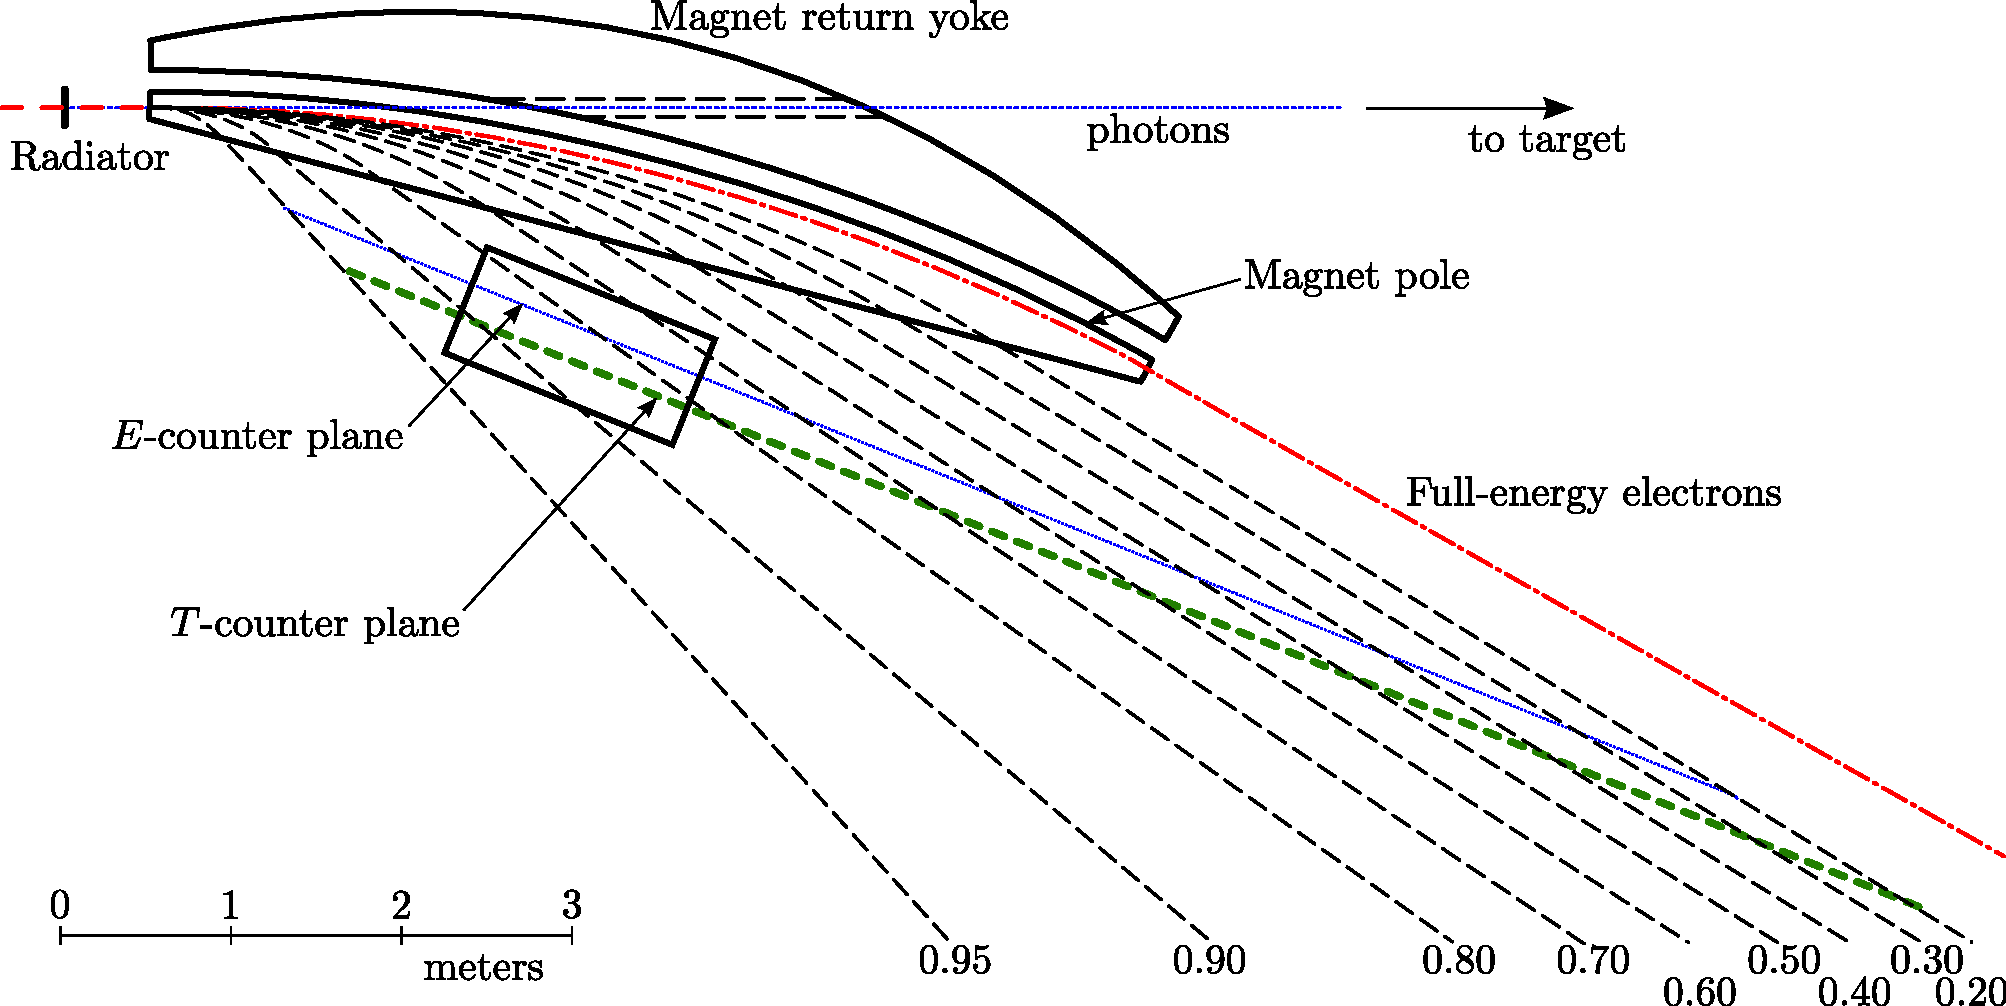
\includegraphics[width=0.8\figwidth,height=\qfigheight]{\grpath/hall-b/tagger_energies.pdf}
\caption[Scale drawing of the photon tagger system]{\label{fig:jlab.tagr.energies}Scale drawing of the photon tagger system. The rectangular area around the $E$ and $T$-counter planes outlines the expanded view shown in Fig.~\ref{fig:jlab.tagr.paddles}.}
\end{center}\end{figure}


\begin{figure}\begin{center}
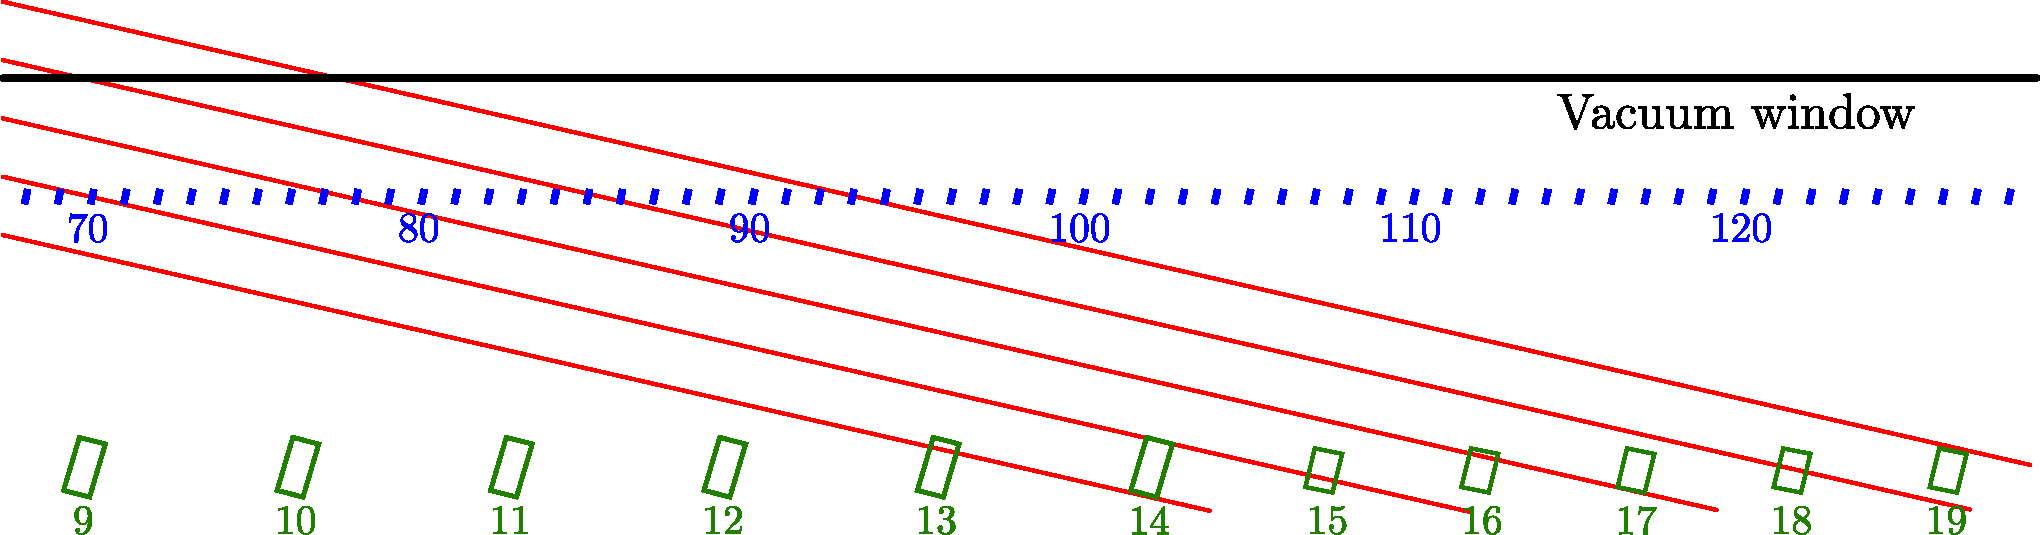
\includegraphics[width=1.1\figwidth,height=\qfigheight]{\grpath/hall-b/tagger_paddles.pdf}
\caption[Scale drawing of the $E$-counters (blue) and the $T$-counters (green) showing examples of recoiled electrons (red lines) entering from the upper left]{\label{fig:jlab.tagr.paddles}{\coloronline}Scale drawing of the $E$-counters (blue) and the $T$-counters (green) showing examples of recoiled electrons (red lines) entering from the upper left.}
\end{center}\end{figure}
\FloatBarrier

\section{CEBAF Large Acceptance Spectrometer (CLAS)} \label{sec:tjnaf.clas}

The \abbr{CLAS} detector, shown in Figs.~\ref{fig:clas}, ~\ref{fig:clas.ced}, is assembled of four types of detectors, five detectors total,  that are arranged in an onion like pattern (around the beam line) covering $\sim 3\pi$ with a diameter of 8~m. Each layer is segmented such that there are six segments around $\phi$ (angle about the beam line), called sectors, each with a polar coverage, $\theta$ (angle from beam line), of approximately $\frac{3}{4}\pi$~radians. Each sector consists of a scintillator start counter (\abbr{ST}) Sec.~\ref{sec:clas.st}, three layers of drift chambers (\abbr{DC}) Sec.~\ref{sec:clas.dc}, a layer of scintillator ``time-of-flight'' counters (\abbr{TOF}) Sec.~\ref{sec:clas.tof}, a gas Cherenkov counter (\abbr{CC}) Sec.~\ref{sec:clas.cc} and an electromagnetic calorimeter (\abbr{EC}) Sec.~\ref{sec:clas.ec}. There is a toroidal magnetic field generated by six superconducting coils that divide the sectors. The direction of the toroidal field is azimuthal, $\phi$ (angle about the beam line), such that the charged particles conserve their azimuthal angle along their trajectory, except near the coils. The magnetic field geometry guides the particles which allows for a simplified reconstruction algorithm to determine the particles' momenta, see Eq.~\ref{eq:motioninmag}. This section will discuss the subsystems in more detail.
% This field however produces an asymmetry in the acceptance of oppositely charged particles. 


\begin{figure}\begin{center}
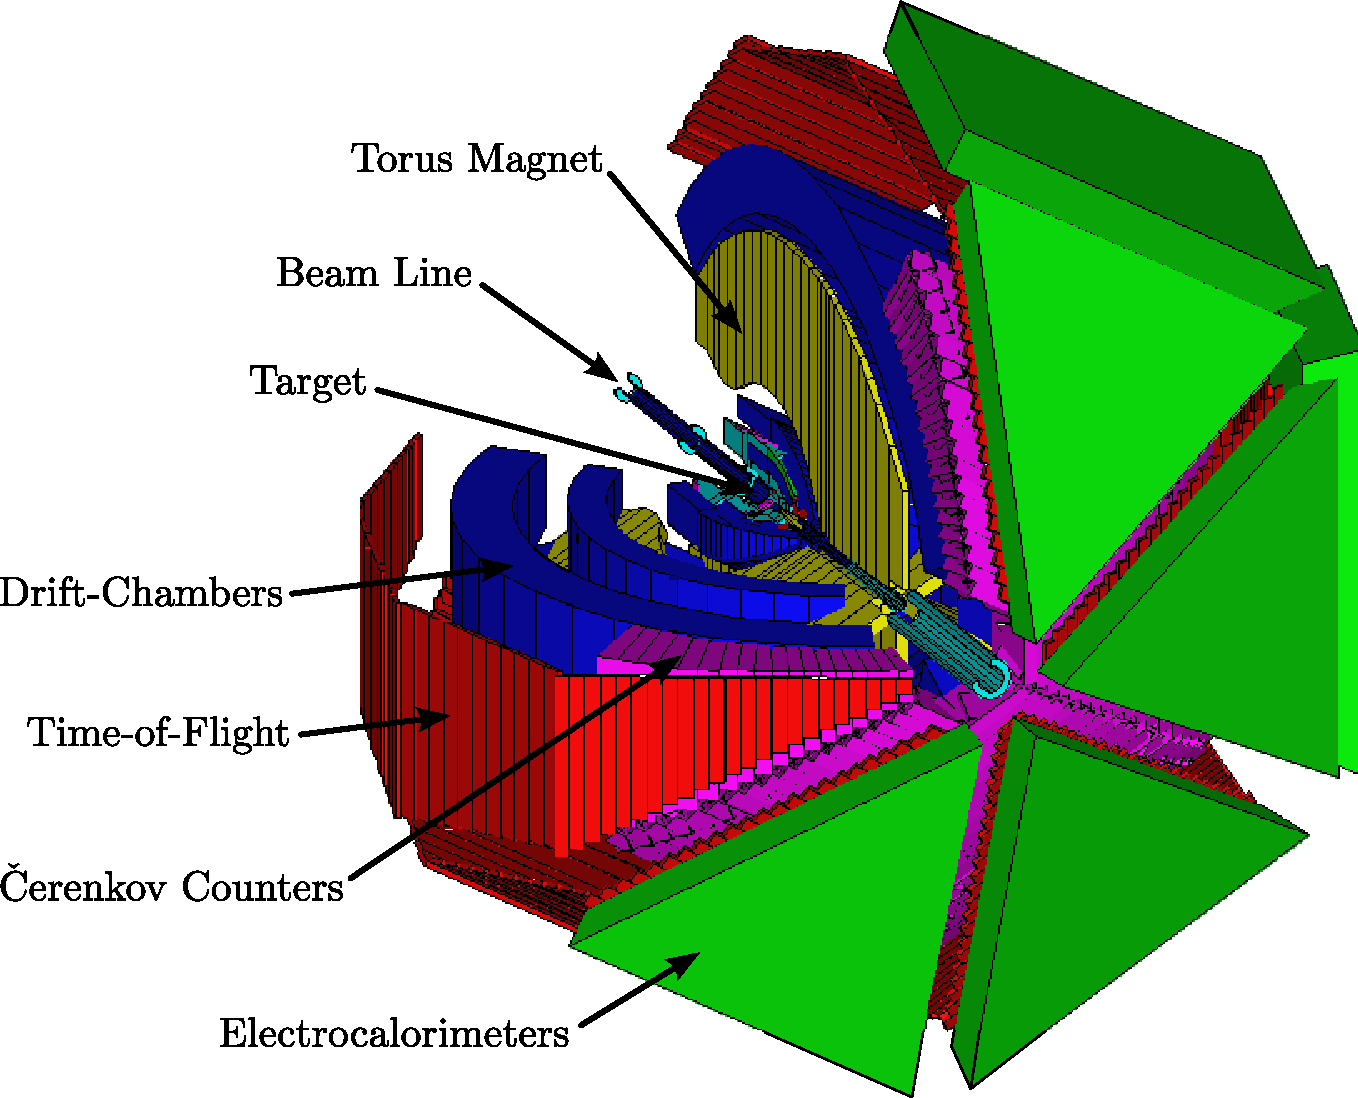
\includegraphics[width=0.8\columnwidth,height=0.75 \hfigheight]{\grpath/hall-b/clas_schematic.pdf}
\caption[Schematic of the \abbr{CLAS} detector with subsystems identified]{\label{fig:clas}{\coloronline}Schematic of the \abbr{CLAS} detector\cite{clas} with subsystems identified. This view is looking upstream and the beam enters from the upper left. The detector is approximately 8~meters in diameter.}
\end{center}\end{figure}

\begin{figure}\begin{center}
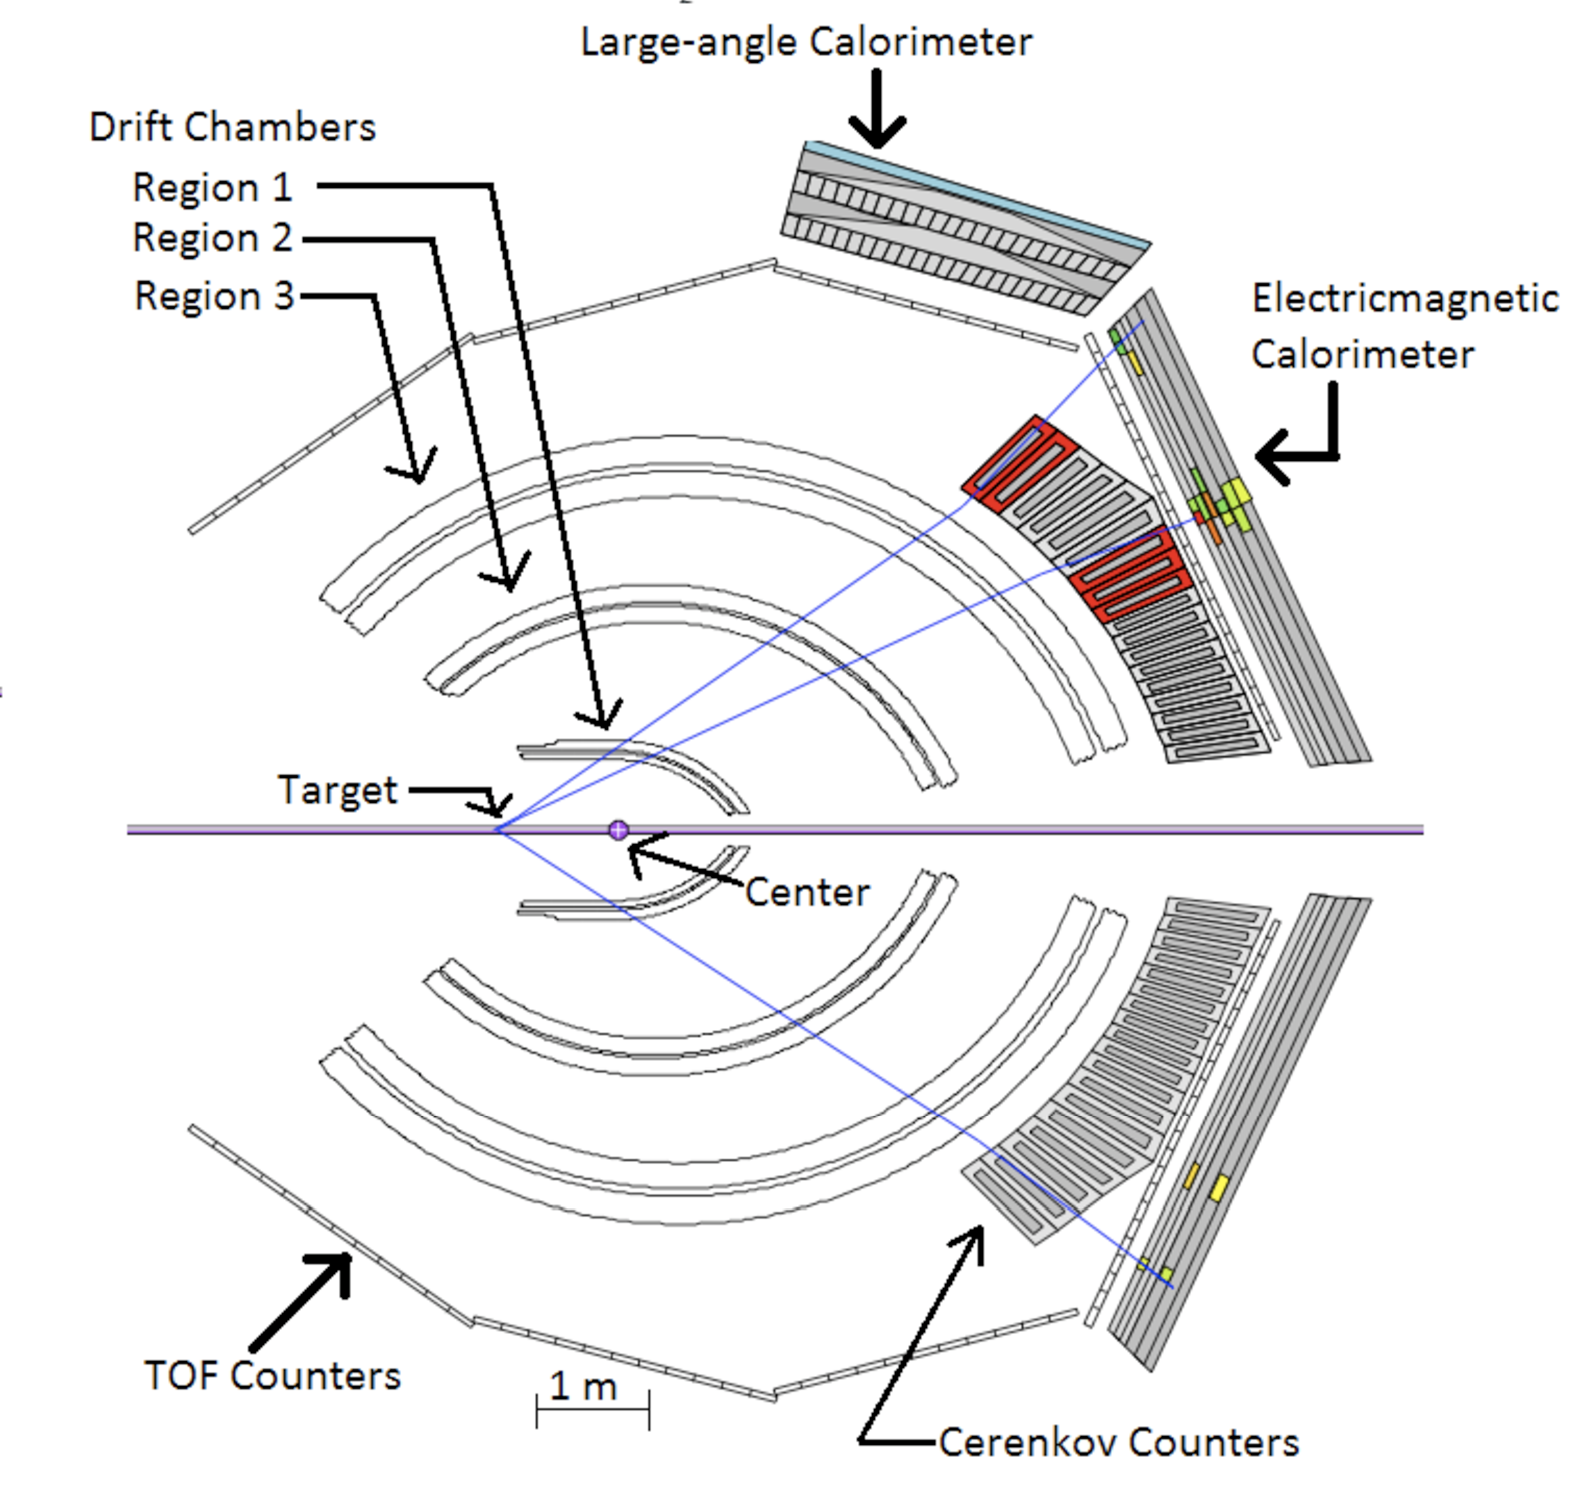
\includegraphics[width=0.6\columnwidth,height=0.75 \hfigheight]{\grpath/hall-b/clas_D.pdf}
\caption[A cross section view of the \abbr{CLAS} detector showing an event with three tracks emanating from the target]{\label{fig:clas.ced}A cross section view of the \abbr{CLAS} detector showing an event with three tracks emanating from the target. The two tracks leaving hit patterns \abbr{CC} and \abbr{EC} are leptons while the track on the bottom panel is a proton}
\end{center}\end{figure}

\begin{figure}\begin{center}
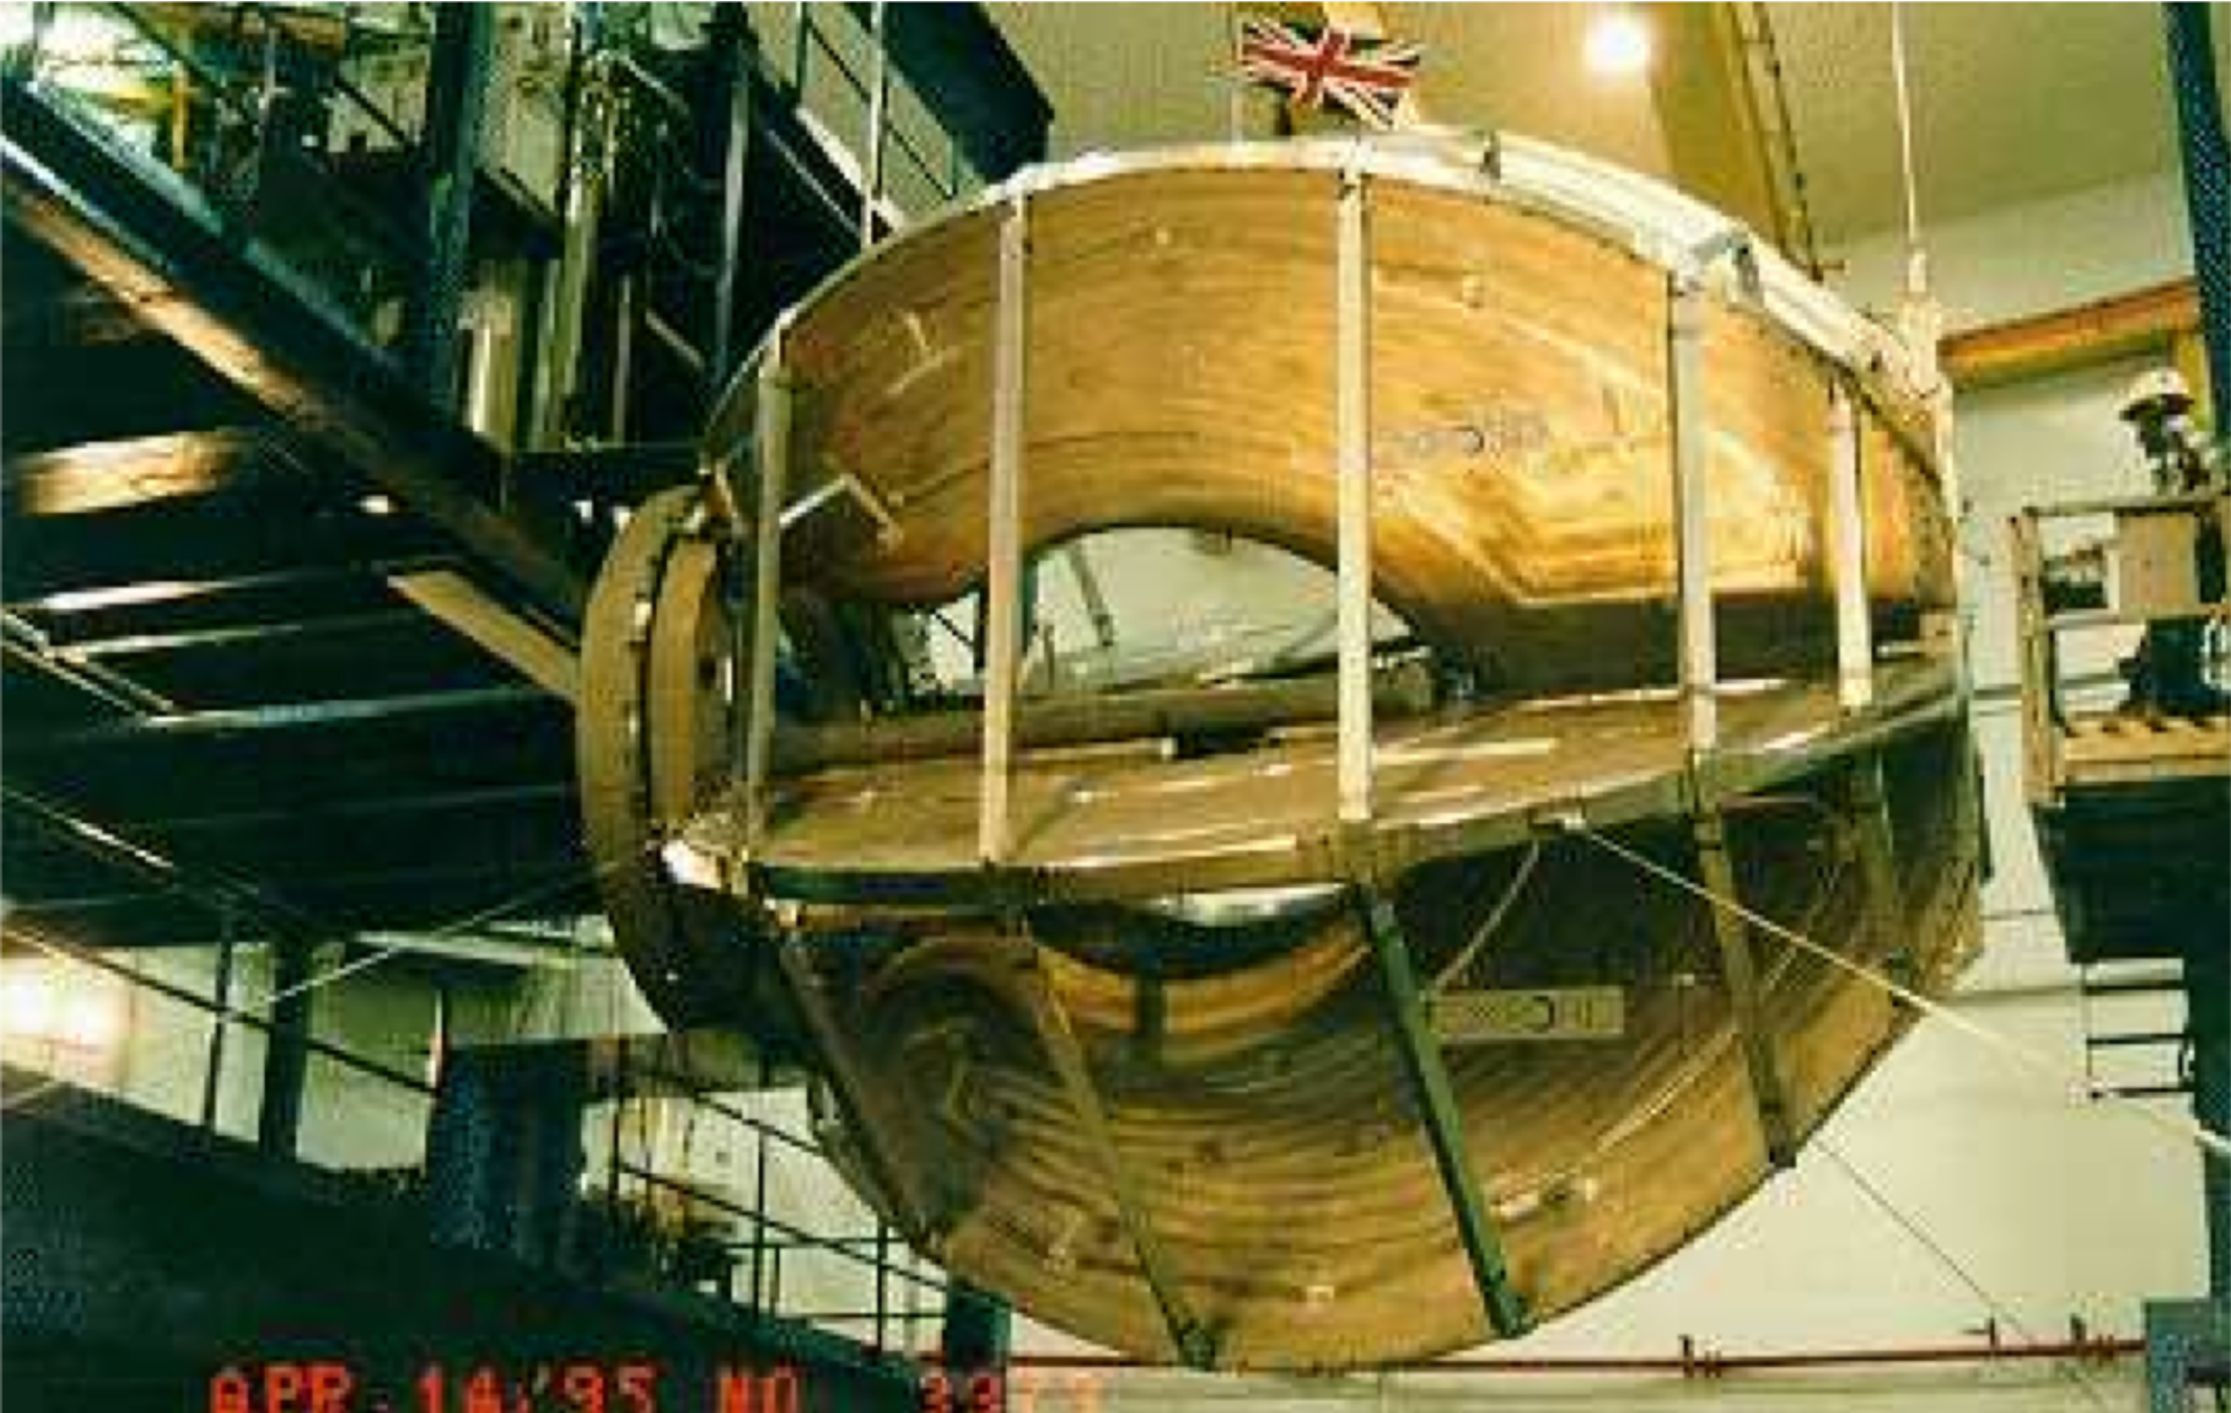
\includegraphics[width=0.55\columnwidth,height=\qfigheight]{\grpath/hall-b/torus_install.pdf}
\caption[The coils of the \abbr{CLAS} toroidal magnet prior to installation of the rest of the detector]{\label{fig:torusinstall}{\coloronline}The coils of the \abbr{CLAS} toroidal magnet prior to installation of the rest of the detector. Image Source~\cite{williams}}
\end{center}\end{figure}
\FloatBarrier

\subsection{Hydrogen Cryotarget}\label{sec:clas.tgt}


The target used by \g12 was conical as shown in Fig.~\ref{fig:clas.targetblueprint}. The target walls were constructed of 0.127~$\mu$m thick Kapton. It is 40~cm in length and 2~cm in radius. The incident photon beam had a radius of 1.5~cm. The target cell design shown in Figs,~\ref{fig:clas.targetblueprint} and~\ref{fig:clas.targetcell} had been used in several experiments and is capable of containing a number of different materials, such as helium, deuterium and hydrogen. For \g12 the target was filled with liquid hydrogen ($\ell$H$_2$). The temperature and pressure of the target was continuously measured and recorded. In Sec~\ref{sec:analysis.target_density}, these measurements will be used to calculate the density of the liquid Hydrogen to determine the target thickness. The target was not polarized.

\begin{figure}[h!]\begin{center}
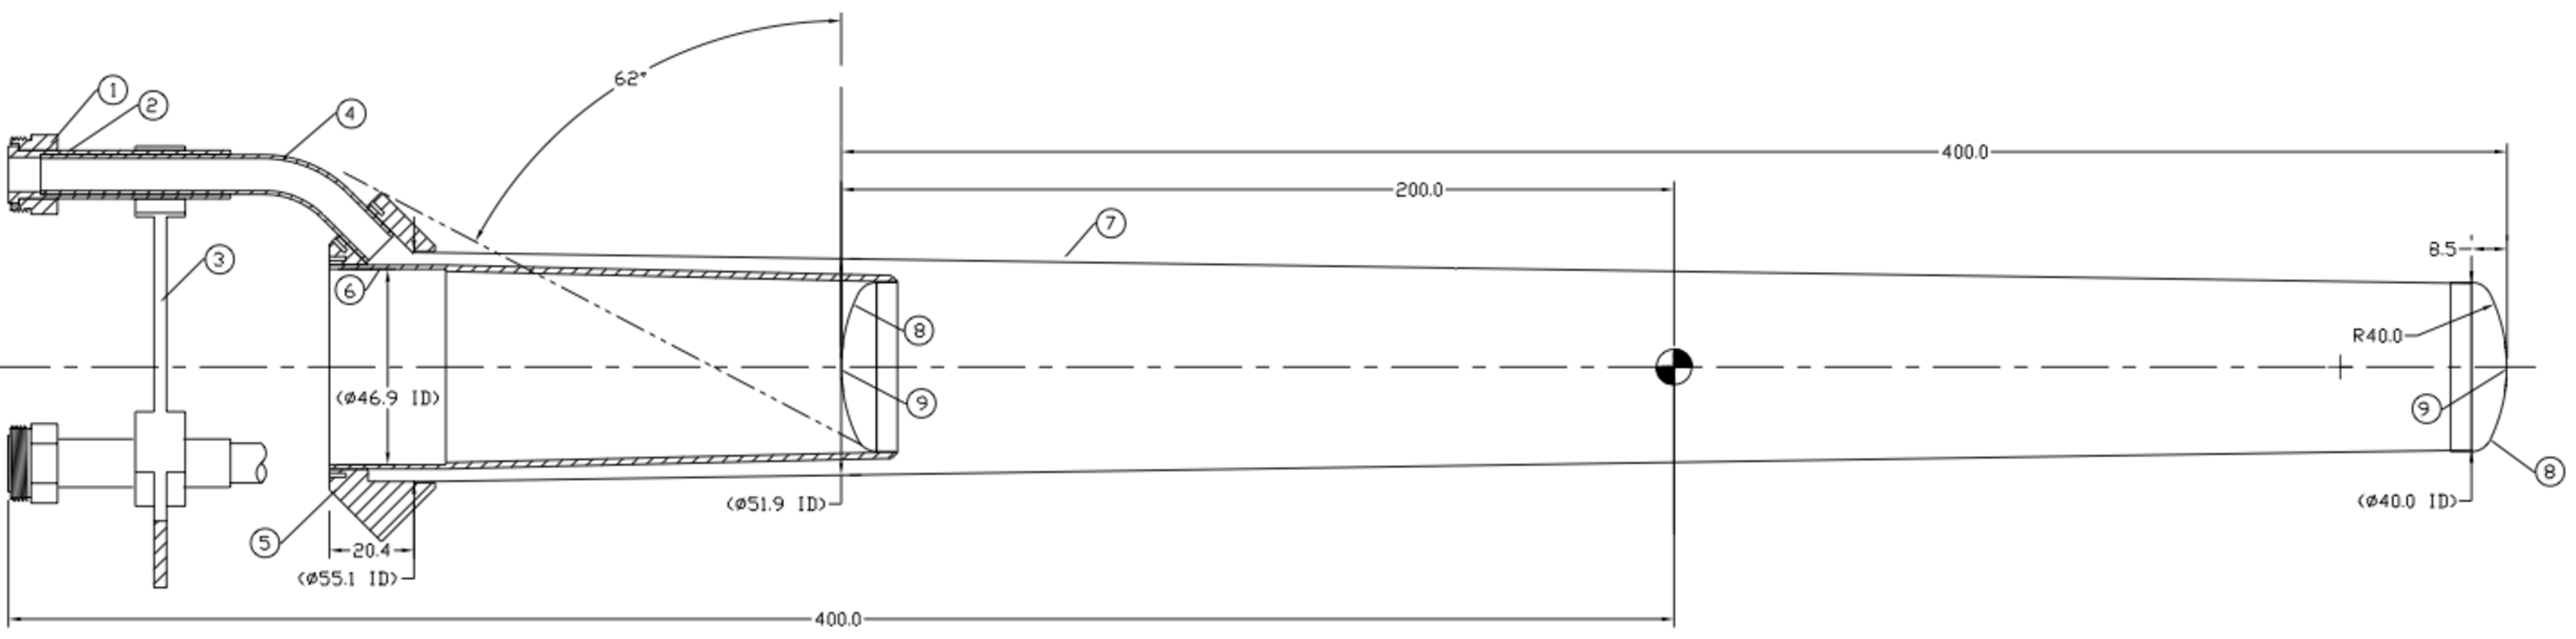
\includegraphics[width=\figwidth,height = \qfigheight]{\grpath/hall-b/g11_target_cell_blueprint.pdf}
\caption[Blueprint schematic of the conical Kapton target cell used for \g12]{\label{fig:clas.targetblueprint}Blueprint schematic of the conical Kapton target cell used for \g12.}
\end{center}\end{figure}

\begin{figure}[h!]\begin{center}
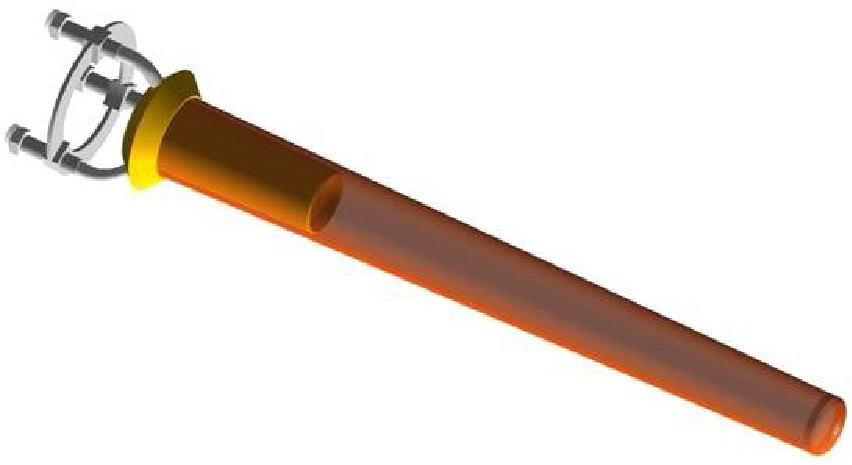
\includegraphics[width=0.6\figwidth]{\grpath/hall-b/g11_target_cell.pdf}
\caption[The 40~cm long conical Kapton target cell used for \g12]{\label{fig:clas.targetcell}The 40~cm long conical Kapton target cell used for \g12.}
\end{center}\end{figure}

%\subsubsection{Target Position for \g12}\label{sec:clas.tgt.position}
The target was located 90~cm upstream of \abbr{CLAS} the center, see Fig.~\ref{fig:clas.ced}.
This increased the forward angle acceptance from 8$^\circ$  to 6$^\circ$. However, this also decreased the large angle acceptance from approximately 140$^\circ$ to 100$^\circ$ in the lab frame.
%This reduction in large angle acceptance sacrificed multi-particle final state events, where the final state particles were more than about 70$^\circ$ away from beamline.
%as well as a reduction in \abbr{DC} resolution. The \abbr{DC} resolution decrease was due to the oblique angle the tracks made with the detector planes.
\FloatBarrier
\section{Start Counter}\label{sec:clas.st}

The start counter, Figs.~\ref{fig:clas.st} and~\ref{fig:clas.stxsection}, is a \abbr{PMT}-instrumented scintillator detector that surrounds the CLAS cryotarget hermetically. It consists of 24 scintillation paddles divided into six sectors matching that of \abbr{CLAS}. Each sector of the start counter is constructed of four independently-instrumented scintillator strips. Timing resolution of the start counter is $\sim$350~ps. The start counter information was used the \g12 triggers~\ref{sec.data.trig.lepton}. More information on the CLAS start counter can be found in \cite{clas.st}.

\begin{figure}[h!]\begin{center}
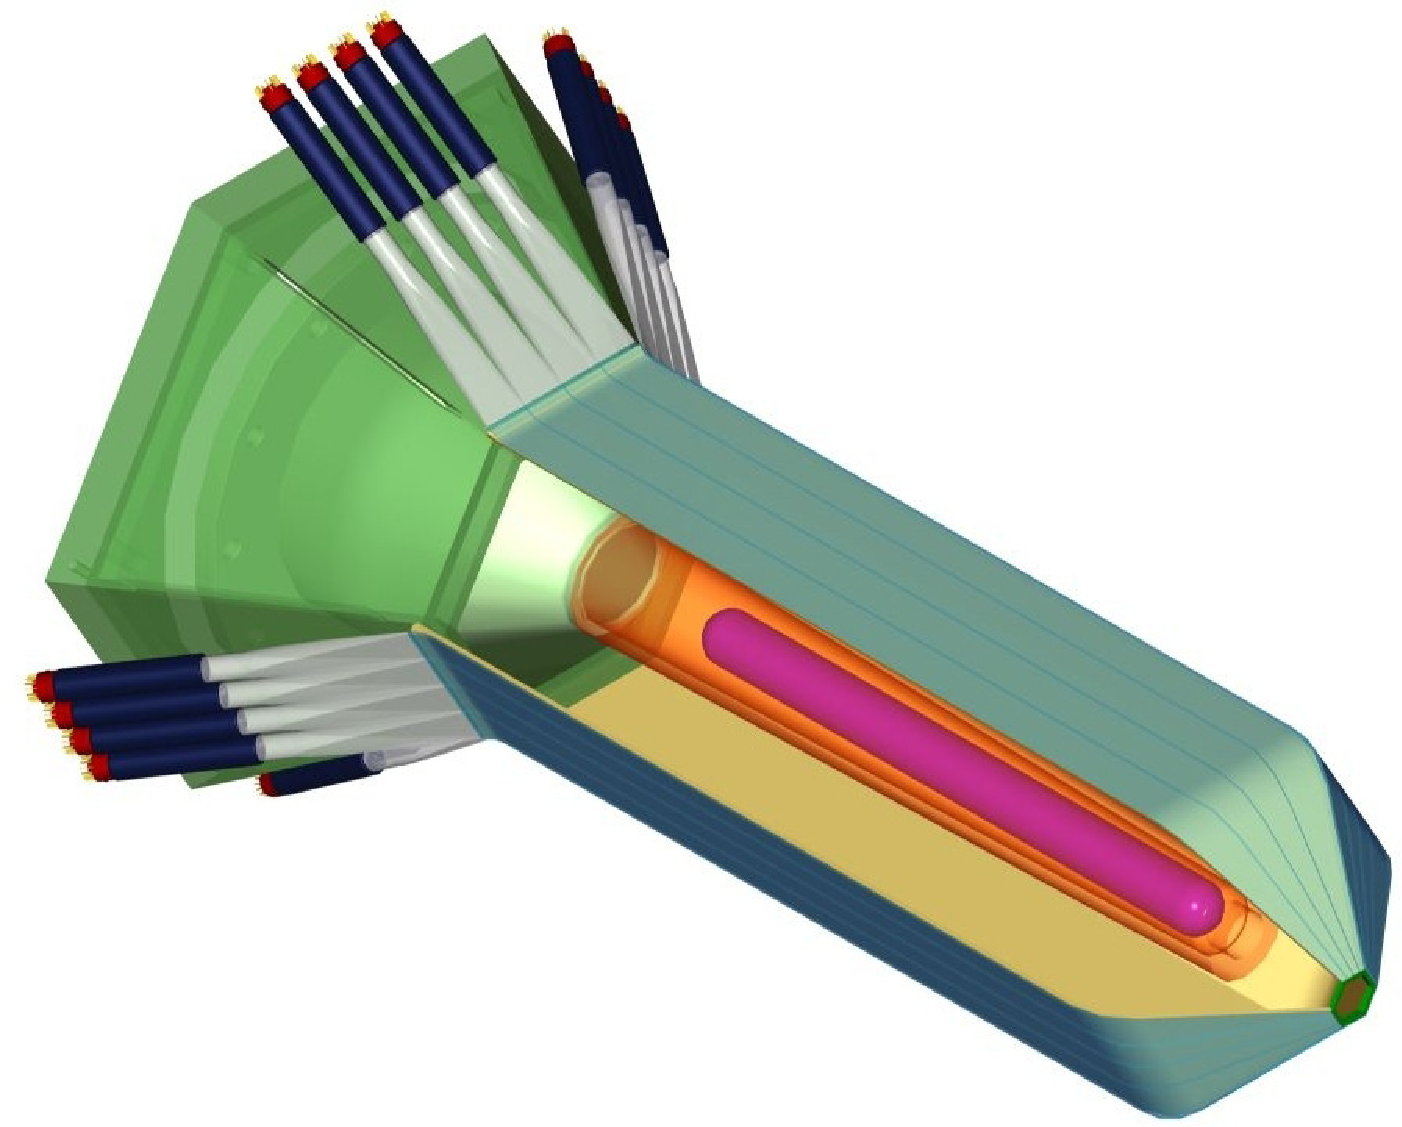
\includegraphics[width=0.8\figwidth,height=\qfigheight]{\grpath/hall-b/start_counter.pdf}
\caption[Schematic of the start counter (\abbr{ST}) with the 40~cm long target cell (purple) at the center]{\label{fig:clas.st}{\coloronline}Schematic of the start counter (\abbr{ST}) with the 40~cm long target cell (purple) at the center. The beam enters from the upper left of the figure.}
\end{center}\end{figure}

\begin{figure}[h!]\begin{center}
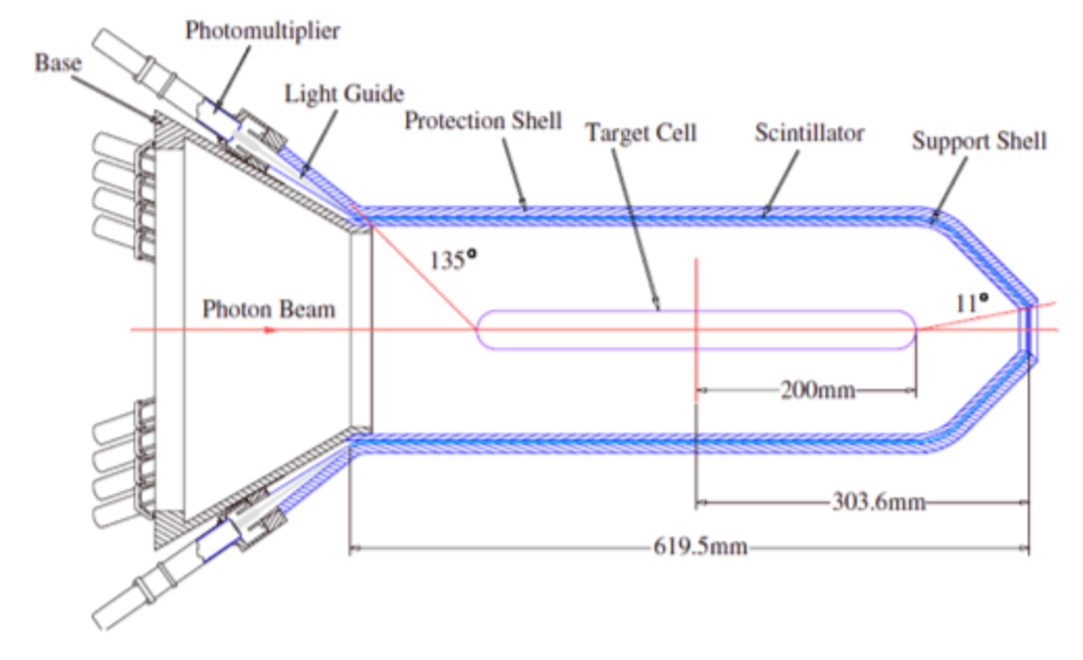
\includegraphics[width=0.8\figwidth,height=\qfigheight]{\grpath/hall-b/start_counter_wtarget.pdf}
\caption[Cross-section view of the start counter illustrating the labeled components and its angular coverage when at the center of \abbr{CLAS}]{\label{fig:clas.stxsection}{\coloronline}Cross-section view of the start counter illustrating the labeled components and its angular coverage when at the center of \abbr{CLAS}.}
\end{center}\end{figure}

\FloatBarrier
%\subsection{Start Counter Efficiency Analysis}\label{sec:clas.st.eff}
%There is an inefficiency of the start counter as seen in Fig.~\ref{fig:classt.ineff}. This inefficiency was measured by using real data events as generated events and passing them through \abbr{CLAS}'s Monete-Carlo package(\abbr{GSIM}\label{abbr:gsim}). More information about this inefficiency will be discussed in Sec.~\ref{sec:analysis.accept.verify}.
%
%%It was observed that 20~\% of the events would fail in simulation, this will be discussed in Sec~\ref{sec:gsim.efficiency}. A portion of the failed events were based upon a failure to reconstruct the required banks for the start counter. This phenomena was investigated from the raw data and found to also be present in the processing of the data from raw to user file in the same manner as seen from Monte-Carlo. The blue-dashed line in Fig.~\ref{fig:classt.ineff} illustrates the start counter inefficiency that is dependent on the events reconstructed vertex. The inefficiency is due to the start counter reconstruction algorithm not being able to link the start counter hit to a track through time-based tracking. This track is not lost due to a reprocess of time-based tracking, linking the track to another particles start counter hit with the same 
%
%%The inefficiency of the start counter is not a mechanical fault but rather the fault of the algorithm used to reconstruct a start counter hit. TO study this raw data events were processed event by event using the program DDD and \abbr{CLAS} event display (\abbr{ced}). Unknown of the cause, it  
%
%
%\begin{figure}[h!]\begin{center}
%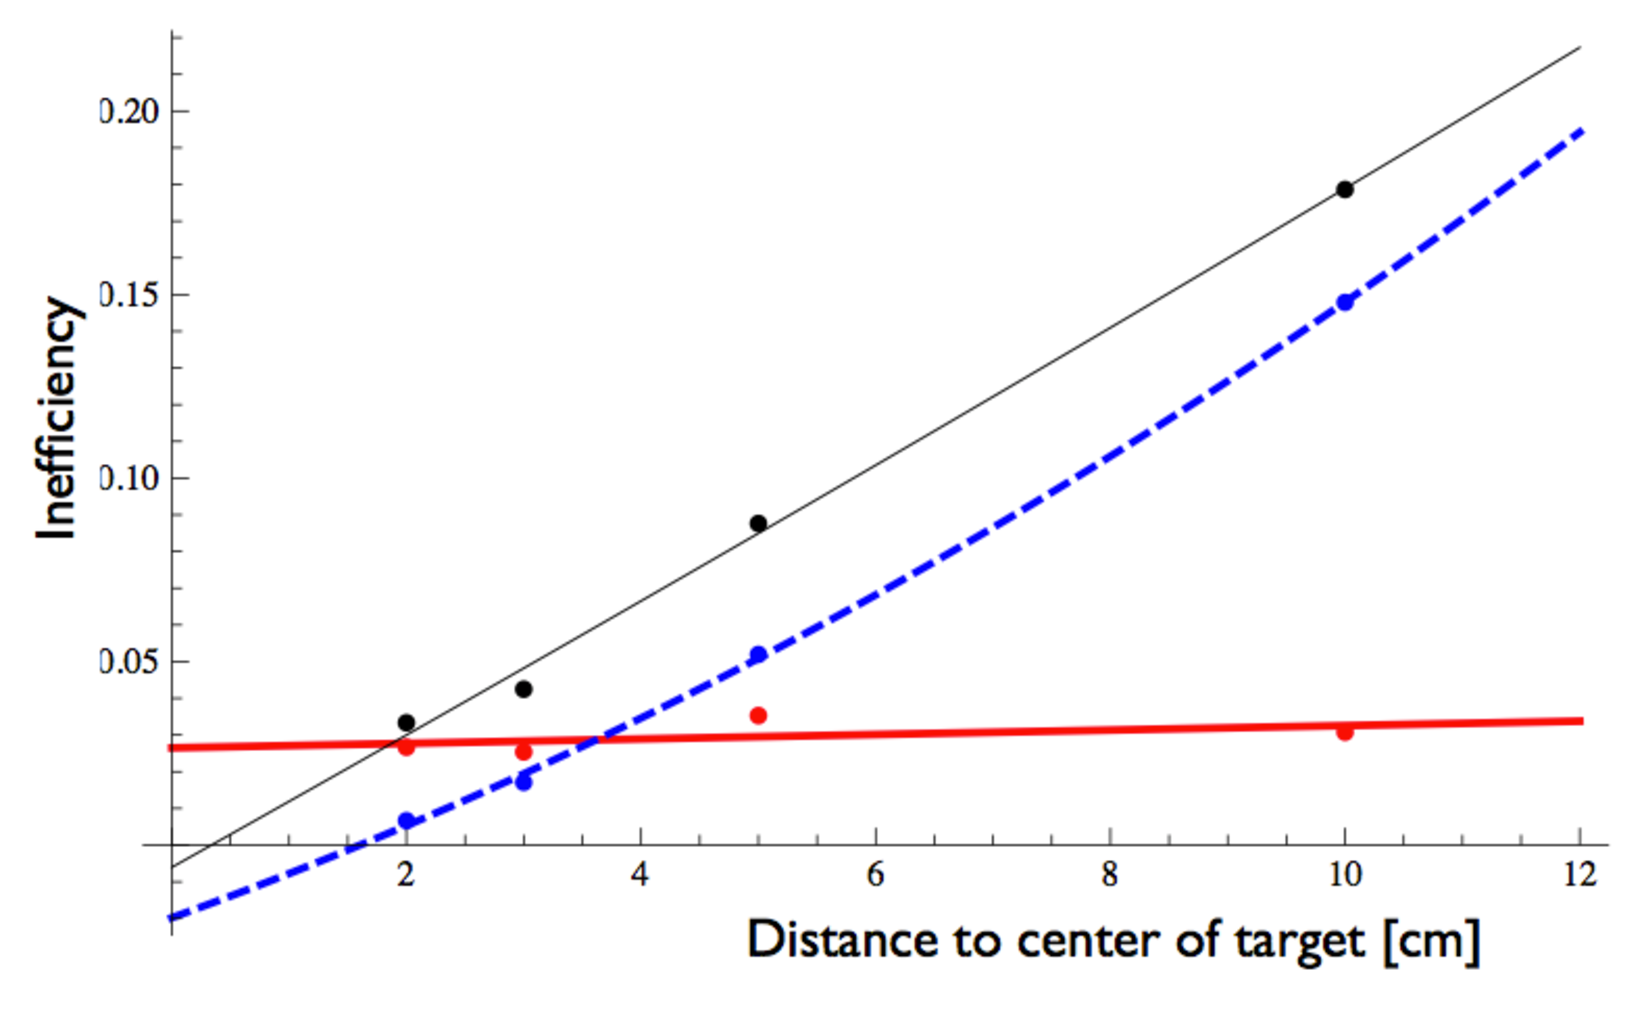
\includegraphics[width=0.8\figwidth,height=0.7\hfigheight]{\grpath/hall-b/st_issue_4_thesis.pdf}
%\caption[Start Counter Inefficiency]{\label{fig:classt.ineff}{\coloronline}Plot showing the inefficiency of the start counter from data events, red-solid line is the inefficiency of reconstruction based solely on hit-based tracking, blue-dashed line is inefficiency of start counter, black-solid is combined. }
%\end{center}\end{figure}
%
%\FloatBarrier
\section{Superconducting Toroidal Magnet}\label{sec:clas.tor}

The essence of \abbr{CLAS} is the use of a toroidal magnetic field generated by six superconducting coils consisting of 4 layers of 54 windings of aluminum-stabilized niobium titanium NbTi/Cu superconductor \cite{clas}. The coils are separated in the azimuthal direction, $\phi$, by 60$^\circ$ and are located between Region-1 and Region-3 of the \abbr{DC}, see Fig~\ref{fig:clas.dc.torus.mag}. The placement of the coils is such that the magnetic field is encompassed by the volume of the \abbr{DC}, see Fig.~\ref{fig:clas.dc.torus.mag}. The direction of the toroidal field points along $\phi$, except near the coils,  such that the charged particles conserve their azimuthal angle along their trajectory, see Fig~\ref{fig:clas.dc.torus.cont}. The maximum current the magnet can support is 3861~A, resulting in a maximum field strength of 35~kG. During the \g12 experiment, the magnets operated at a current of 1930~A corresponding to a maximum field of about 20~kG. The field was oriented such that positive charged particles bent away from the beam-line, while negative charged particles bent toward the beam-line. Running at higher currents provides better momentum resolution but decreases the detector's acceptance for negative particles. Knowing the strength and direction of the magnetic field and the trajectory of a particle using the \abbr{DC}, the particle momentum can be determined by use of Eq.~\ref{eq:motioninmag}.
% During the \g12 experiment, the magnet was cooled down to 4.5~K using liquid helium ($\ell$He) obtained from the central CEBAF central cryogenic facility.

\begin{figure}[h!]\begin{center}
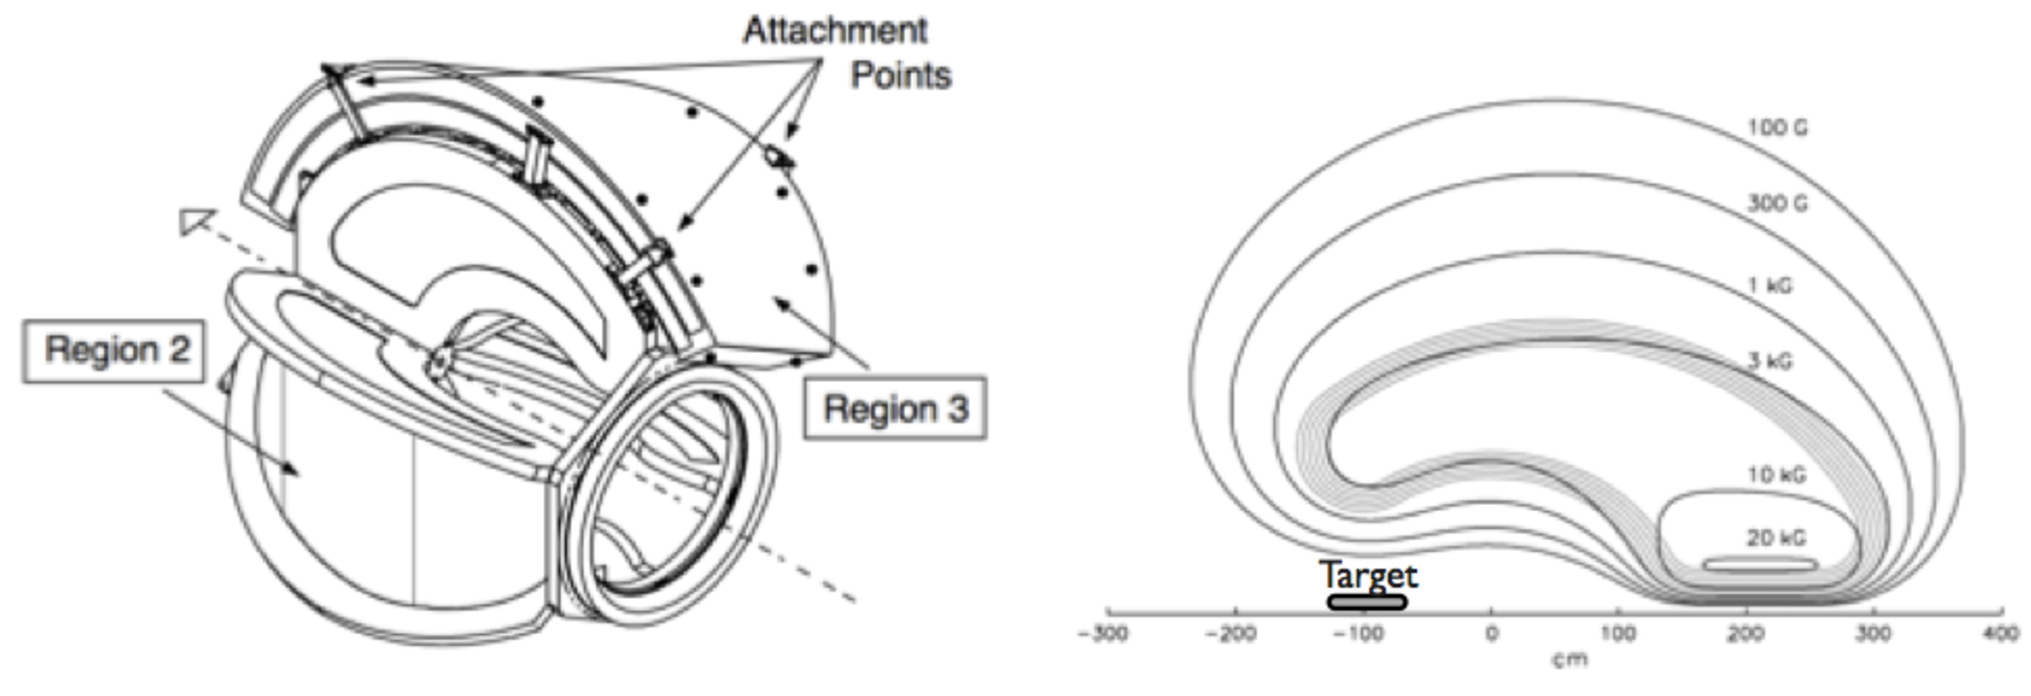
\includegraphics[width=\figwidth,height=0.9\qfigheight]{\figures/hall-b/torus_field_mag_mount.pdf}
\caption[The \abbr{CLAS} Superconducting Toroidal Magnet and its placement in relation to Region-1 and Region-3]{\label{fig:clas.dc.torus.mag}The \abbr{CLAS} Superconducting Toroidal Magnet and its placement in relation to Region-1 and Region-3  (left). Cross-section of the \abbr{CLAS} Superconducting Toroidal Magnet at half current (1930~A). Region-2 of the \abbr{DC} is located inside the region of the coils shown as the kidney shaped loop at about 3~kG (right).}
\end{center}\end{figure}

\begin{figure}[h!]\begin{center}
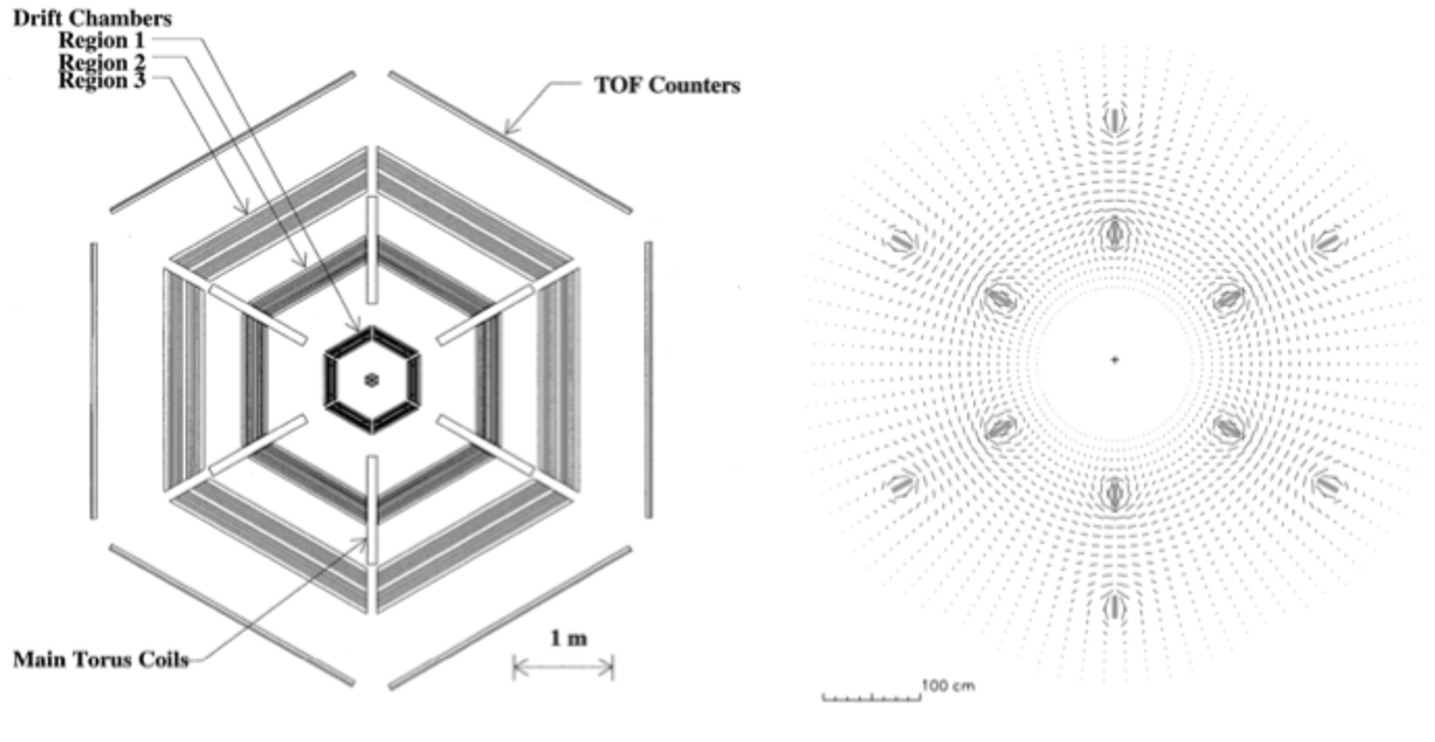
\includegraphics[width=1.\figwidth,height=0.75\hfigheight]{\figures/hall-b/torus_field_and_DC.pdf}
\caption[Schematic cross-sectional view of the \abbr{CLAS} detector, perpendicular to the beam line]{\label{fig:clas.dc.torus.cont}Schematic cross-sectional view of the \abbr{CLAS} detector, perpendicular to the beam line (left). The magnetic field distribution corresponding to the view in the left figure. The field is purely azimuthal. The six torus coils are shown in grey, the field is in the counter-clockwise direction,  the field strength is concentrated in the region between the coils (right).}
\end{center}\end{figure}

\FloatBarrier
\section{Drift Chambers}\label{sec:clas.dc}

The \abbr{CLAS} drift chambers \abbr{DC} (Figs.~\ref{fig:clas},~\ref{fig:clas.dc.torus.cont},~\ref{fig:clas.dc.drift}) track charged particles above 200~MeV/c with polar angle resolution of 2-4~mrad and momentum resolution of 0.5 - 1\%, depending on momentum, see Fig~\ref{fig:clas.dc.res}. Typical coverage of the \abbr{DC} is $8^\circ < \theta < 142^\circ$, when the target is at \abbr{CLAS} center. For the \g12 experiment the coverage of the \abbr{DC} was modified to $6^\circ < \theta < 100^\circ$ due to the placement of the target, see Sec~\ref{sec:clas.tgt} for reasons explained in ~\cite{clas.proposal.hyclas},~\cite{clas.proposal.superg},~\cite{clas.proposal.pion}.
\begin{figure}\begin{center}
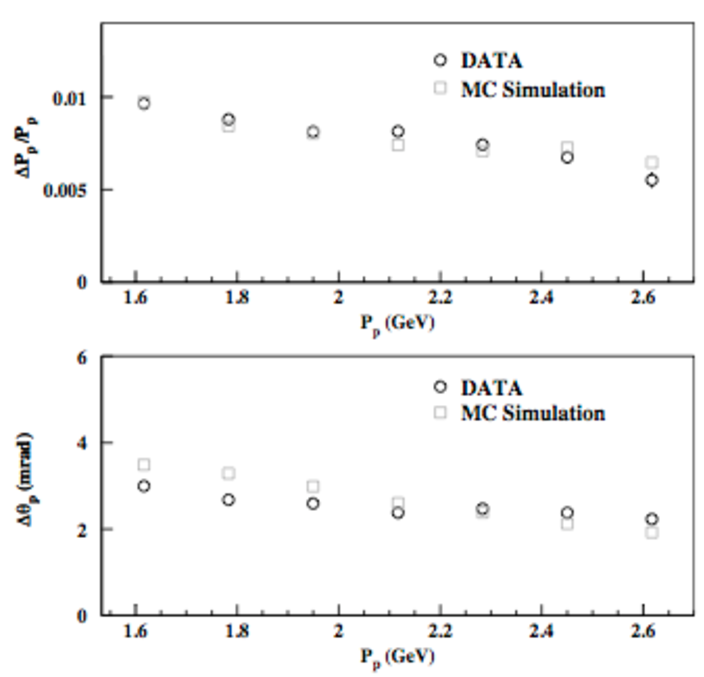
\includegraphics[width=0.8\figwidth,height=0.75\hfigheight]{\figures/hall-b/drift_DC_resolution.pdf}
\caption[Momentum and angular resolution for protons as determined from the measured angle of the scattered electron for data collected and Monte-Carlo simulation]{\label{fig:clas.dc.res}Momentum and angular resolution for protons as determined from the measured angle of the scattered electron for data collected and Monte-Carlo simulation. Image Source~\cite{clas}}
\end{center}\end{figure}

The \abbr{DC} are divided into six sectors each containing three radial layers (Fig.~\ref{fig:clas.dc.drift}), referred to as ``Regions'', for a total of 18 separate drift chambers. Each \abbr{DC} region covers the same polar angular range and consist of two superlayers which each contain six layers of hexagonal wire cells which house evenly spaced 20~$\mu$m gold-plated tungsten sense wires (center of hexagon) each surrounded by six 140~$\mu$m gold-plated aluminum alloy field wires (vertices of hexagon). In the first superlayer, the wires are strung approximately parallel to the direction of the magnetic field (axial wires), while the second superlayer has wires tilted at a 6$^\circ$ angle with respect to the axial wires (stereo wires). A high voltage system maintains the sense wires at positive potential, while the field wires are maintained at a negative potential 50\% lower than the positive value. The difference of potentials creates an avalanche of the electrons induced by the ionizing particle. The hexagonal shape of the cell mimics a circular geometry cell in which the drift time to drift distance is independent of entrance angle.

The inner region is denoted as Region 1. Its first superlayer has only 4 layers due to space constraints. Region 1 is nearly free from magnetic field, see Fig~\ref{fig:clas.dc.torus.mag}. Region 2 is situated between the magnetic coils which is subject to the highest magnetic field which is used to determine the particle's curvature, needed to determine the particle;s momenta, see Eq.~\ref{eq:motioninmag}. Region 3 purpose is to provide global track reconstruction in connection with other CLAS detectors since Region 3 is located outside the volume of magnetic field. Each \abbr{DC} is filled with a gas mixture of 90\% argon and 10\% carbon-dioxide. This choice of gas provides high drift velocity (0.04 m/$\mu$sec) and fast collection time which improves momentum resolution. For more information on the design of the \abbr{CLAS} \abbr{DC} system, see~\cite{clas.dc} and for more information on the calibration process of the \abbr{CLAS} \abbr{DC} system, see~\cite{clas.dc.calib}.

\begin{figure}\begin{center}
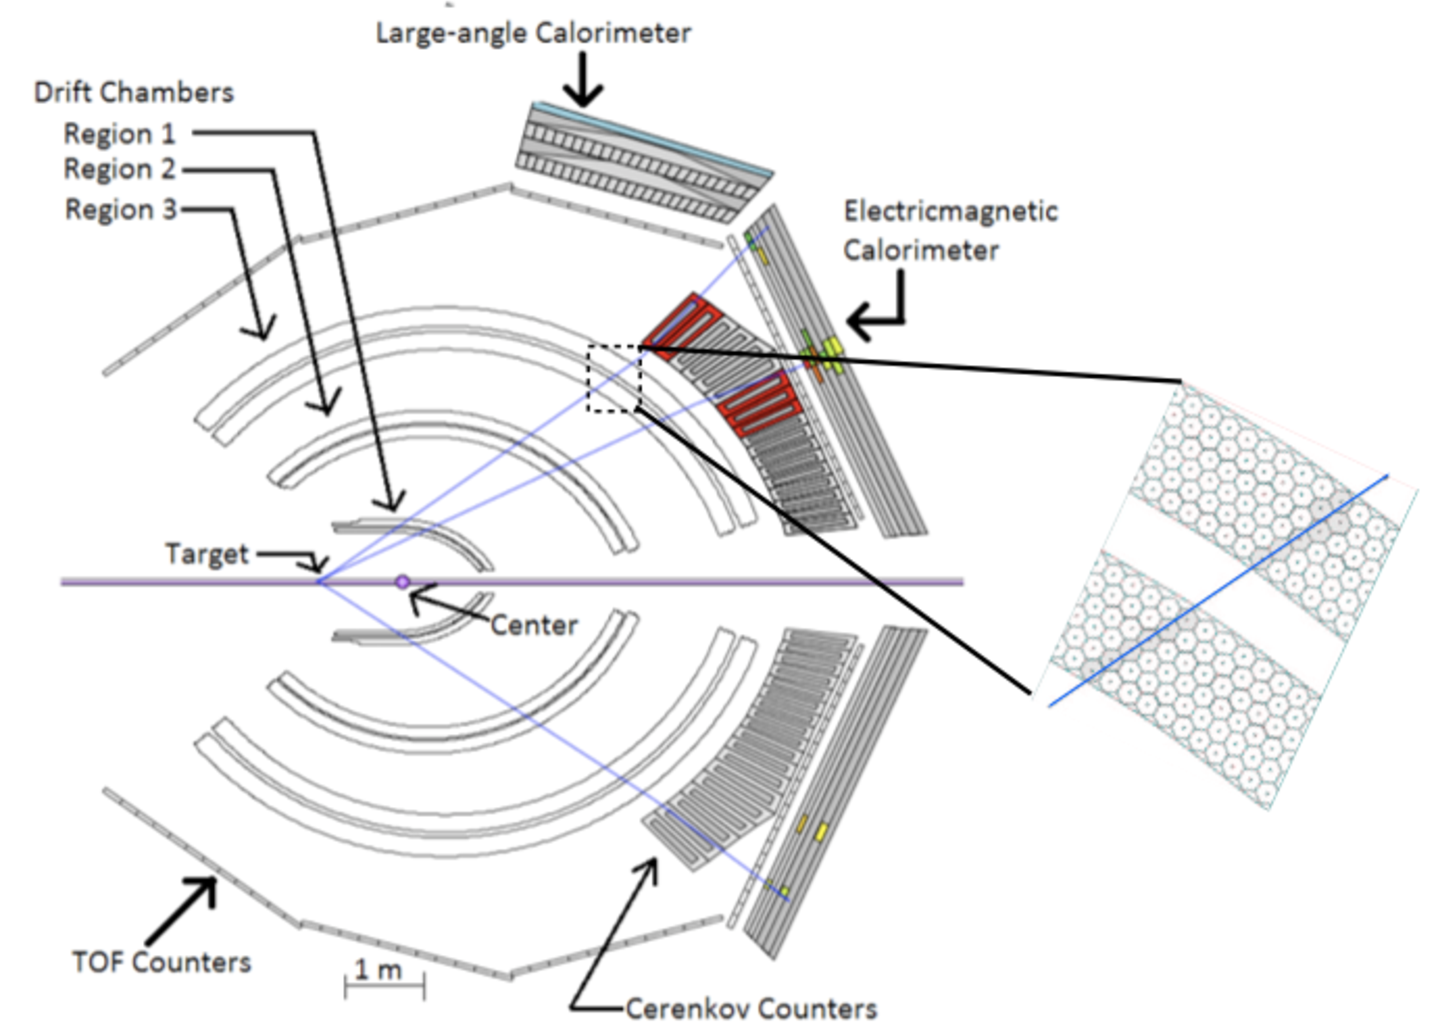
\includegraphics[width=\figwidth,height=0.75\hfigheight]{\figures/hall-b/drift_DC_cedII.pdf}
\caption[A cross section view of the \abbr{CLAS} detector showing an event with three tracks emanating from the target]{\label{fig:clas.dc.drift}A cross section view of the \abbr{CLAS} detector showing an event with three tracks emanating from the target. The two tracks leaving hit patterns \abbr{CC} and \abbr{EC} are leptons while the track on the bottom panel is a proton. The inlet shows hexagonal cells of drift chambers with a typical track indicated by shaded areas for the cut-out in Region-3.}
\end{center}\end{figure}

\FloatBarrier
\section{Cherenkov Radiation and Detectors}\label{sec:clas.cc}

When a charged particle traverses through a medium with a velocity less than the speed of light for that medium ($v < c/n$) the dipoles of the molecules in the medium are symmetrically arranged such that the integrated dipole field along the particles path vanishes. However, when the particles speed is greater than that of the speed of light for that medium the dipoles of the molecules arrange themselves such that they are asymmetric along the particles path and thus creates a dipole field, see Fig~\ref{fig:clas.cc.dipole}.
\begin{figure}[h!]\begin{center}
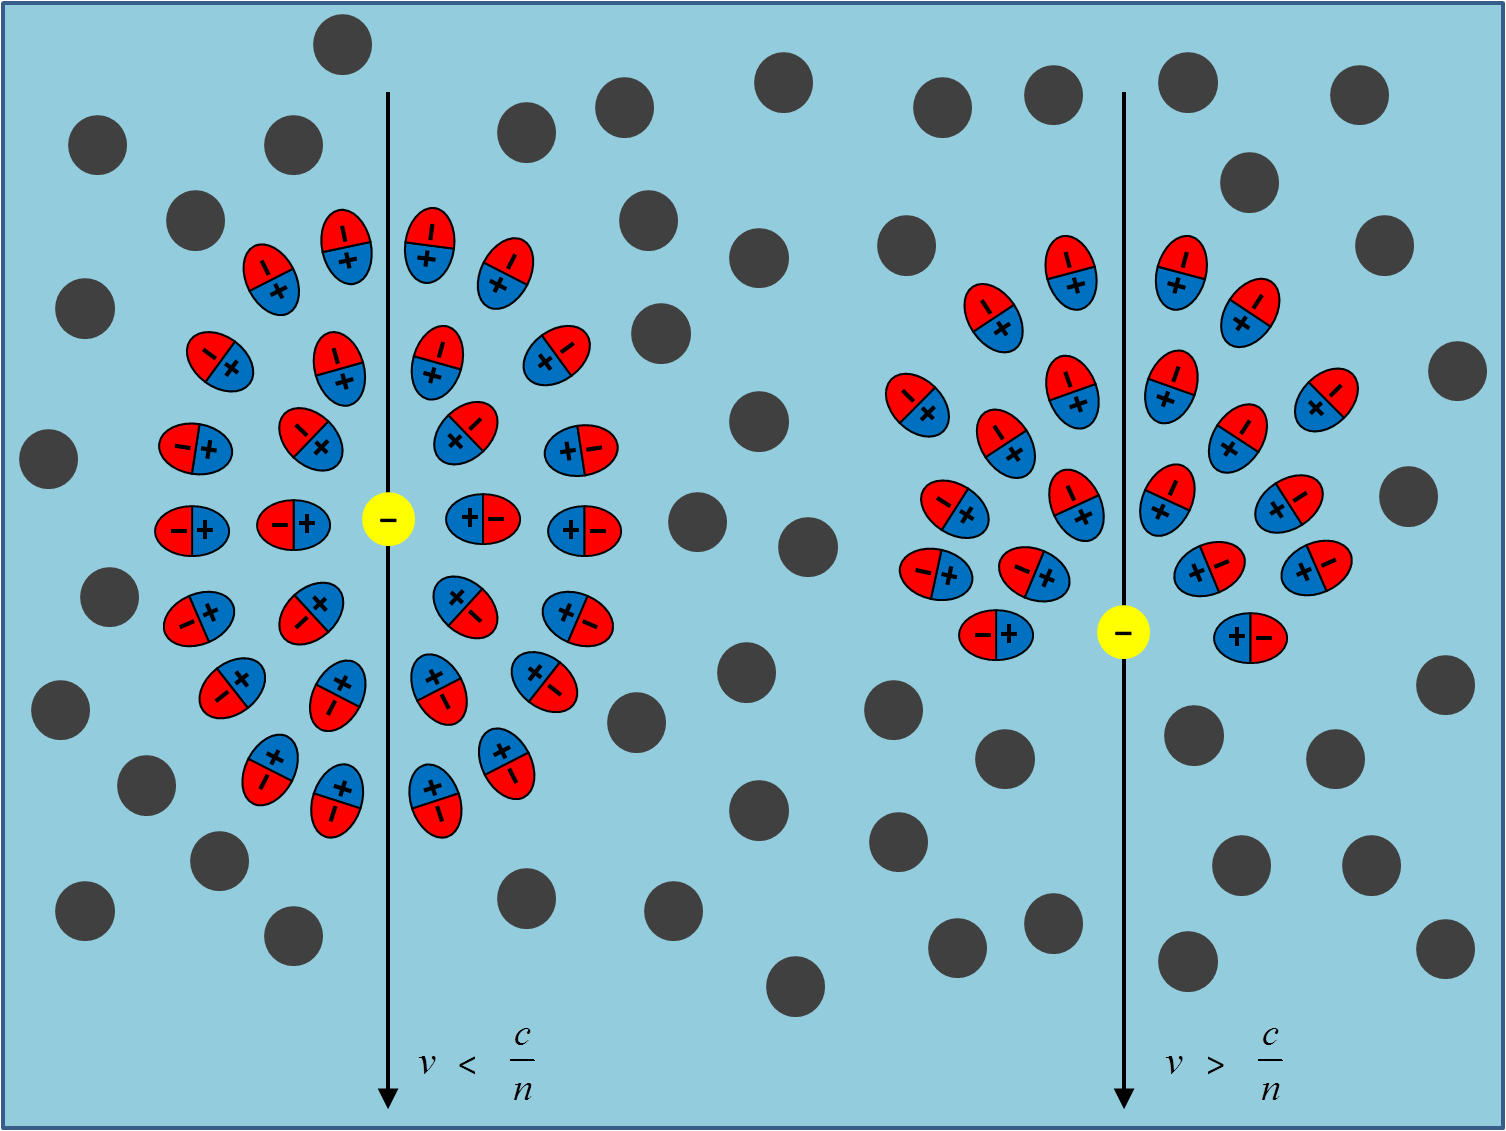
\includegraphics[width=\figwidth,height=\qfigheight]{\figures/hall-b/CCECPLOTS/cherenkov.pdf}
\caption[Illustration of Cherenkov Radiation]{\label{fig:clas.cc.dipole}Illustration of Cherenkov Radiation. Negative charged particle traveling through a medium with $v < c/n$ showing dipoles symmetrically arranged around particles path (left). Negative charged particle traveling through a medium with $v > c/n$ showing dipoles asymmetrically arranged around particles path given rise to dipole field(right). Image Source:~\cite{cherenkov_image}}
\end{center}\end{figure}

The generated dipole field radiates the energy contained in this disturbance producing a coherent shockwave, this is known as Cherenkov radiation. An analogy of this phenomena is the sonic boom created in air from an object traveling faster then the speed of sound. Just as the sound wave of a sonic boom travels slower than the traveling object, so does the light emitted from the dipole field. This reduction in velocity creates the wave front of a continuous light spectrum, see Fig~\ref{fig:clas.cc.angle}.
\begin{figure}[h!]\begin{center}
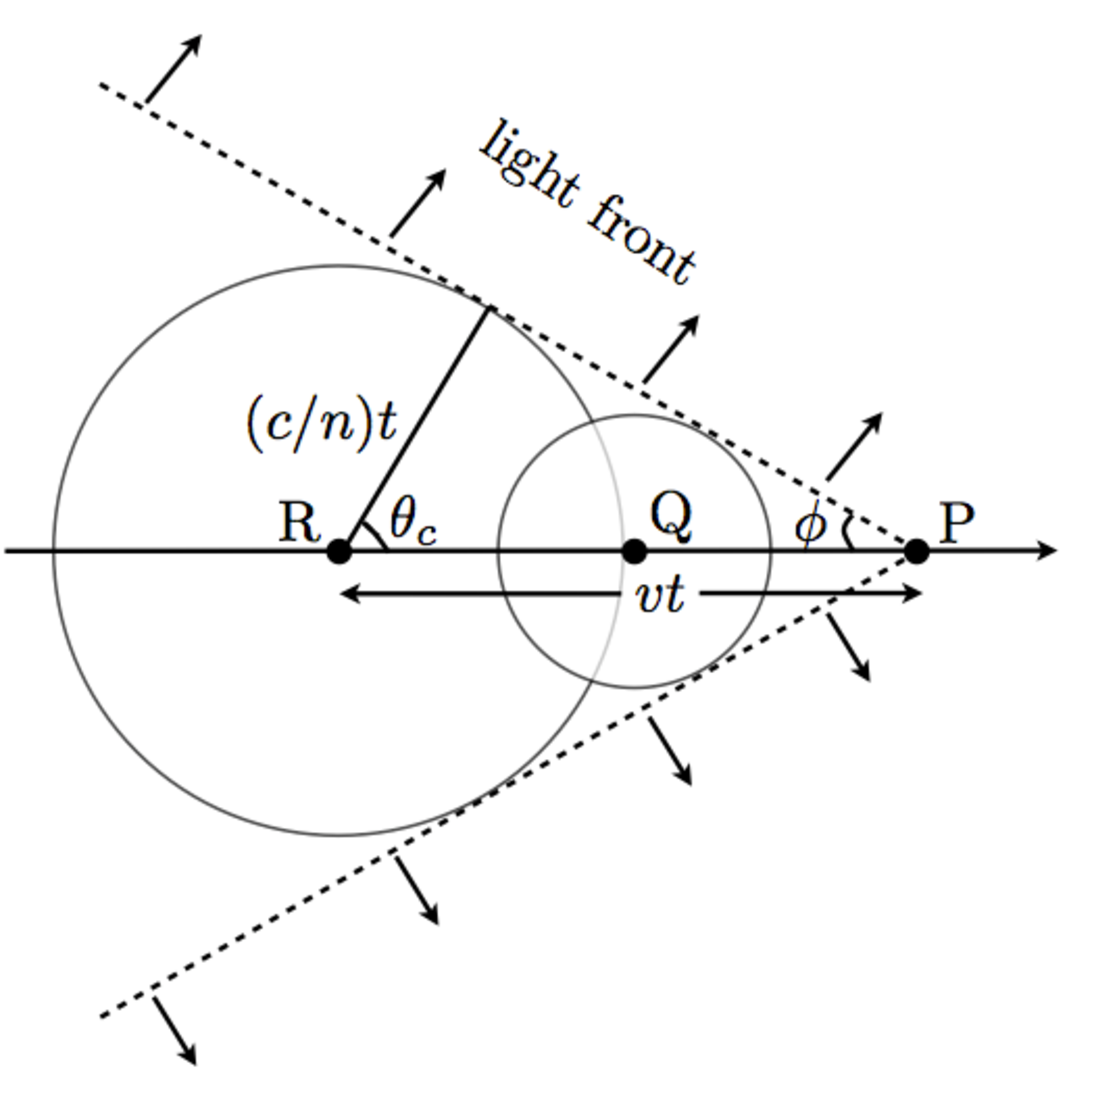
\includegraphics[width=\figwidth,height=0.75\hfigheight]{\figures/hall-b/CCECPLOTS/cc_wavefront_madeII.pdf}
\caption[Illustration of Cherenkov Angle]{\label{fig:clas.cc.angle}Illustration of Cherenkov Angle. When the particle has traveled the distance $\mathrm{RP =\nu t \rightarrow \beta c t}$, the photon (light front) has traveled $(c/n)t$.}
\end{center}\end{figure}

Inspecting Fig~\ref{fig:clas.cc.angle}, when the particle has traveled the distance $\mathrm{RP =\nu t = t \beta c}$, the photon has traveled $(c/n)t$, therefore
\begin{equation}\label{eq:cherenkov_eq}
 \mathrm{\cos\theta_{c} = \frac{(c/n)t}{t \beta c} = \frac{1}{n\beta}}
\end{equation}
and the threshold of Cherenkov radiation is 
\begin{equation}\label{eq:cherenkov_threshold}
 \mathrm{\beta_{th} > \frac{1}{n}}.
\end{equation}
Adding in quantum effects
\begin{equation}\label{eq:cherenkov_eq_quantum}
\mathrm{cos\theta_{c} = \frac{1}{n\beta} + \frac{\Lambda}{\lambda}\frac{n^{2} -1}{2n^{2}}}
\end{equation}
where
\begin{equation}\label{eq:cherenkov_eq_quantum_lambda}
\mathrm{\Lambda = \frac{\sqrt{1-\beta^{2}}}{\beta}\lambda_{0}} \ , 
\end{equation}
$\mathrm{\lambda =}$ wavelength of light in medium, and $\mathrm{\lambda_{0} }$ is the Compton wavelength 0.024 \AA. For practical cases, and using \abbr{CLAS}, the 2$^{nd}$ order term is negligible (n=1.00153). To illustrate that quantum effects are negligible, an electron traveling at threshold in \abbr{CLAS} \abbr{CC},
\begin{equation}
\mathrm{\beta_{th} > \frac{1}{n}} > 0.998472,
\end{equation}

\begin{equation}
\mathrm{\frac{\Lambda}{\lambda}\frac{n^{2} -1}{2n^{2}} =  1.07874 \cdot 10^{-9}}
\end{equation}
%

In \abbr{CLAS}, the Cherenkov counter (\abbr{CC}) is used to detect electrons and positrons while rejecting pions for momenta less than 2.5~GeV. The gas used in the \abbr{CC} for \g12 is perfluorobutane (C$_4$F$_{10}$) with an index of refraction of 1.00153. The threshold energy for producing Cherenkov radiation in C$_4$F$_{10}$ is
\begin{align}
\mathrm{E_{th} = \gamma_{th} m_{0}} \mathrm{ \ (Units \ of \ c)} \\
\mathrm{\gamma_{th} = \frac{n}{\sqrt{n^{2} -1}}} = 18.09
\end{align}
therefore the threshold energy of e$^{\pm}$ is 9.23~MeV while the threshold energy of $\pi^{\pm}$ is 2.52~GeV.
%
The number of photons emitted per unit length at threshold for electrons or positrons is;
\begin{align}\label{eq:cc.NPE}
\frac{dN}{dx} = 2\pi z^2 \alpha \frac{\sin \theta_{c}^2}{\lambda^2} d\lambda = 0.241246 \frac{d\lambda}{\lambda^2}
\end{align}
where $\alpha$ is the fine structure constant, $z =1$ for electrons and positrons, and $\lambda$ is the wavelength at which the photon is emitted. Table~\ref{tab:cc_npe} lists the number of photons/cm for various wavelengths of light for the midpoint of $\beta_{th}$ and a maximum velocity $\beta =1$. Table~\ref{tab:cc_npe} also lists the mirror reflectivity for that wavelength.
\input{tables/cc_nphotons}

The \abbr{CC} subsystem is physically located in the space between Region 3 of the \abbr{DC} subsystem and the \abbr{TOF} in the forward region covering polar angles 8$^\circ$ to 45$^\circ$ in each sector when the target is at \abbr{CLAS} center. For \g12 since the target was placed 90~cm upstream, the polar coverage was approximately from 6$^\circ$ to 35$^\circ$ in the lab frame. The \abbr{CLAS} \abbr{CC}'s were fabricated as 6 independent identical sectors, with each sector divided into 18 regions of $\mathrm{\theta}$, and each $\mathrm{\theta}$ segment divided into 2 modules. Light from Cherenkov radiation is focused in $\mathrm{\phi}$ thus preserving information on the lepton polar angle $\theta$. The optical element of \abbr{CC} module comprises an assembly of one elliptical and one hyperbolic mirror providing primary light focusing into a  ``Winston" light collection cone, a  cylindrical mirror used to compensate for imperfections in the focusing, and a photomultiplier used to count the  number of photons in the light cone, see Fig~\ref{fig:clas.cc_array}. More information on the \abbr{CLAS} Cherenkov detector can be found in~\cite{clas.cc} 

The use of the \abbr{CC} was not included in the original proposals, however a significant drop in price on C$_4$F$_{10}$ just prior to the start of \g12 allowed the gas to be added at the last minute. The price drop was due to the recent availability of another, much cheaper gas that was demonstrated to have the same general properties as C$_4$F$_{10}$ and when \g12 contacted the original supplier of the C$_4$F$_{10}$ for a price match, they committed. 

\begin{figure}[h!]\begin{center}
\subfloat[]{
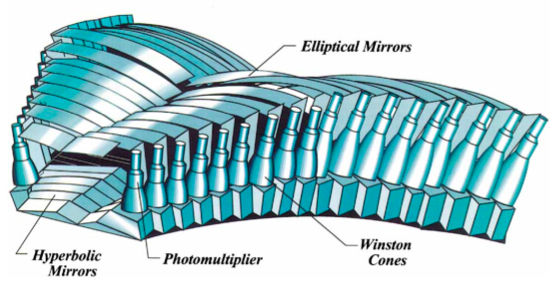
\includegraphics[width=\figwidth,height=0.5\hfigheight]{\figures/hall-b/CCECPLOTS/CCarray}\label{fig:clas.cc_array}
}\\
%[Schematic of one \abbr{CC} showing the 18 symmetrical, mirrored segments of the CLAS \abbr{CC}]
\subfloat[]{
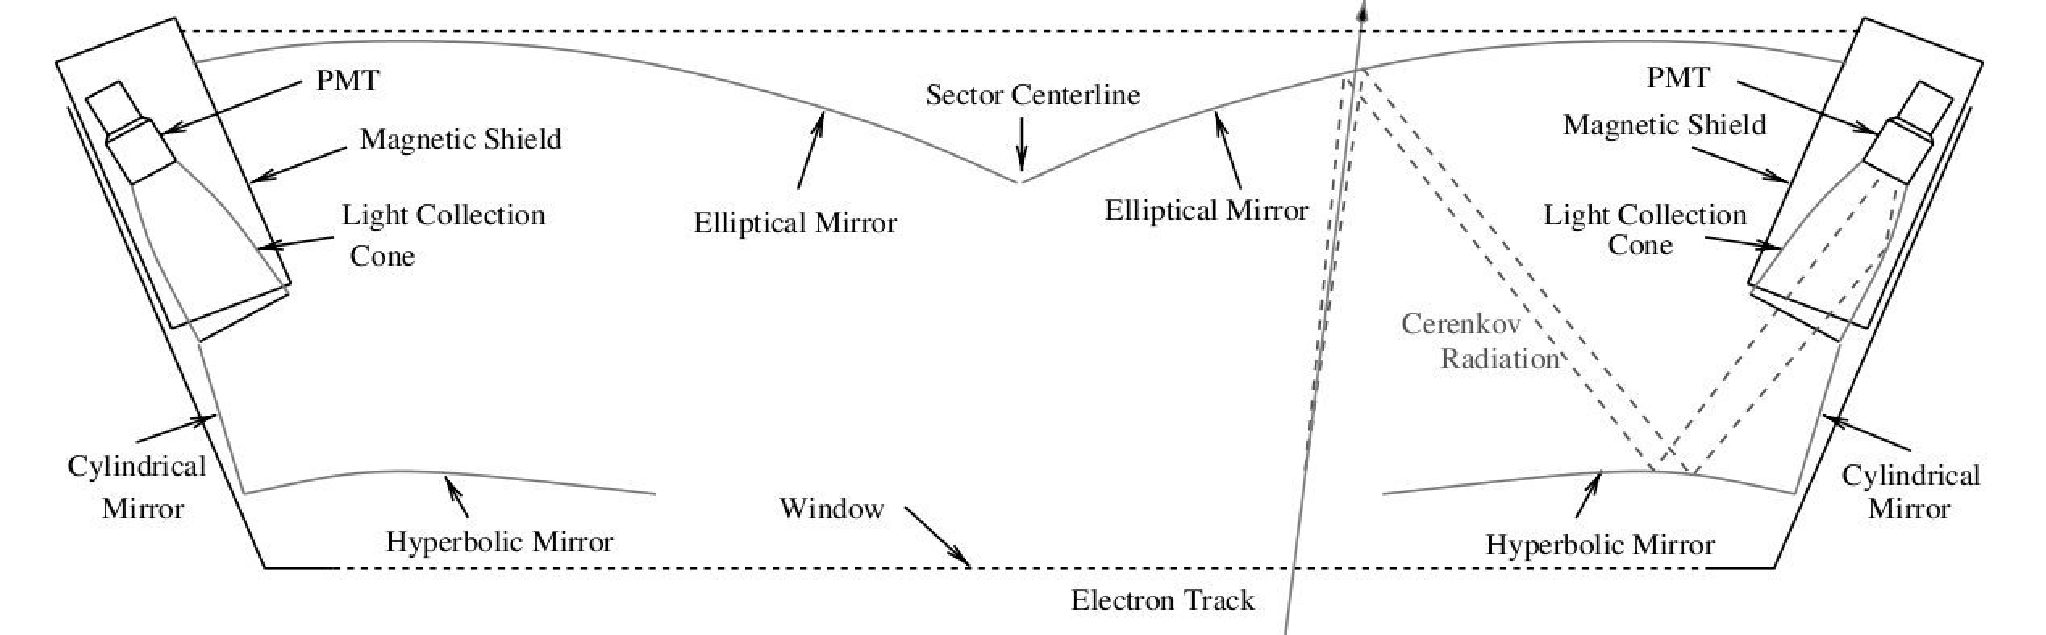
\includegraphics[width=0.9\columnwidth]{\figures/hall-b/cc_diagram.pdf}\label{fig:clas.cc}
}
\caption[Schematic of one \abbr{CC} showing the 18 symmetrical, mirrored segments of the CLAS \abbr{CC}]{Schematic of one \abbr{CC} showing the 18 symmetrical, mirrored segments of the CLAS \abbr{CC}~(a). Diagram of one segment of the Cherenkov counters with an electron entering from the bottom~(b).}

\end{center}\end{figure}






\FloatBarrier
\section{Time-of-Flight Detectors}\label{sec:clas.tof}

The \abbr{CLAS} time-of-flight \abbr{TOF} subsystem provides precise timing measurements of charged particles that transverse the \abbr{CLAS} detector to help determine the particle masses. The \abbr{TOF} subsystem was also used in the \g12 level 1 trigger (see Sec.~\ref{sec:data.trig}) to identify track candidates. The \abbr{TOF} is constructed of organic plastic scintillant (Bicron BC-408). Scintillation is a process undergone by material when radiation traverses a medium.
%
% At room temperature, all valence electrons of the scintillating material are in the $\mathrm{S_{0}}$ ground state. As a particle propagates through the material the incident radiation populates $\mathrm{S_{1}}$ states. Vibrational levels within $\mathrm{S_{1}}$ band decay radiation-less to $\mathrm{S_{1}}$  base states, which in turn decays under emission of light to the $\mathrm{S_{0}}$ band. The radiation-less decay from the excited $\mathrm{S_{1}}$ band to the ground $\mathrm{S_{1}}$ band is known as internal degradation and is responsible for the transparency of the scintillators to their own radiation. $\mathrm{S_{1}}$ can also decay to adjacent triplet levels however, this decay is highly forbidden by multipole selection rules. If this decay does occur, the decay energy is lower causing the decay time to be longer, see Fig.~\ref{fig:clas.scint_bands} for the illustration of this process. Depending on the properties of the scintillator, decay of fluorescent state in organic plastic scintillators have a typical time between 1-3~ns
%
%%\begin{figure}[h!]\begin{center}
%%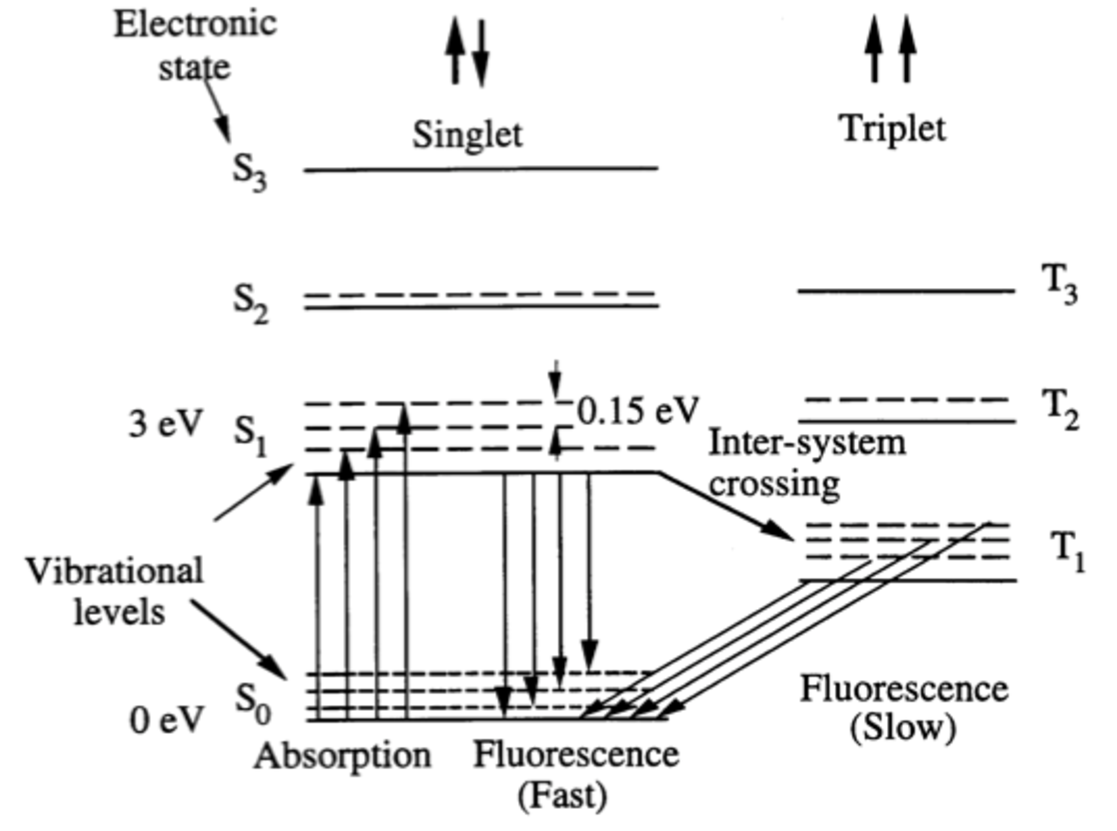
\includegraphics[width=\figwidth,height=0.5\hfigheight]{\figures/hall-b/CCECPLOTS/Calorimetry/scint.pdf}\label{fig:clas.scint_bands}\caption[Typical Energy Levels of scintillating material ]{Diagram of scintillating population of states. Image Source~\cite{vibe_levels}}
%%\end{center}\end{figure}
%\begin{figure}[h!]\begin{center}
%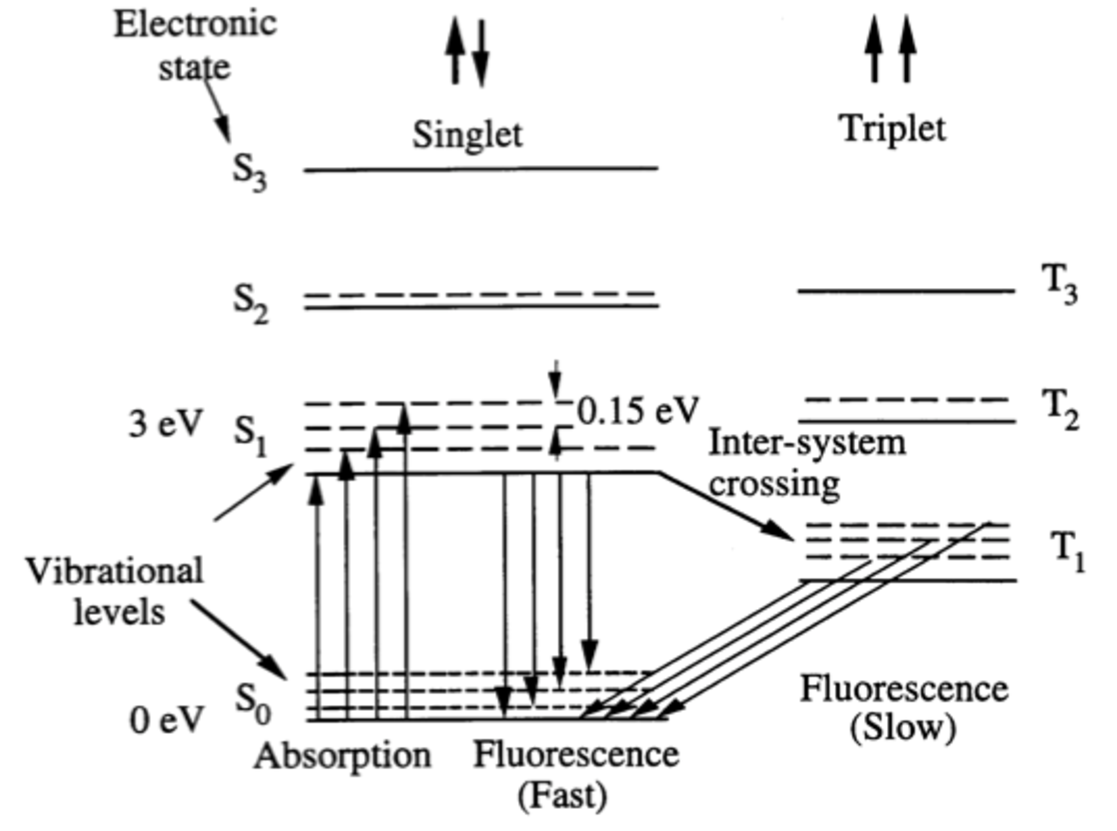
\includegraphics[width=\figwidth,height=0.5\hfigheight]{\figures/hall-b/CCECPLOTS/Calorimetry/scint.pdf}
%\caption[Typical Energy Levels of scintillating material ]{\label{fig:clas.scint_bands}Diagram of scintillating population of states. Image Source~\cite{vibe_levels}}
%\end{center}\end{figure}

The \abbr{TOF} subsystem is located between the \abbr{CC} and \abbr{EC} subsystems approximately 4~m from \abbr{CLAS} center, 5~m from the \g12 target. Each sector 57 scintillator paddles divided into two subgroups. The first subgroup subtends angles of 8.6$^\circ$ to 45.9$^\circ$ and consists of 23 scintillating paddles that are 15~cm in width. Each paddle is instrumented with two 2-in diameter \abbr{PMT}'s, see Fig~\ref{fig:clas.tof.paddles}. The first group was optimized for timing resolution while being cost-effective and covering a large area. The second group consists of 34 paddles that are 22~cm wide, covering polar angles from 45.9$^\circ$ to 142$^\circ$. Each paddle in this range is instrumented with two 3-in diameter \abbr{PMT}'s. All paddle bars are 5.08~cm thick for 100\% detection of minimum-ionizing tracks and a timing resolution of 150--200~ps.
%These forward angle counters \abbr{PMT}'s have a 15.9~cm$^2$ photocathode area which covers the 76.2~cm$^2$ cross-sectional area of the scintillator.
%These large angle counter \abbr{PMT}'s have a 30.2~cm$^2$ photocathode area which covers the 118.8~cm$^{\mathrm{2}}$ cross-sectional area of the scintillator.
\abbr{TOF} information is used to reconstruct a particle's mass is by measuring the difference between the event RF corrected start time and the time measured by the \abbr{TOF}, $t_{stsc}$. The RF corrected start time is the radio-frequency time (RF) from the accelerator beam aligned withe the event start time. Using this time, $t_{stsc}$, the length of trajectory to the \abbr{TOF}, $l_{stsc}$, and the speed of light $c$, the particles' velocity can be calculated as
\begin{equation}\label{eq:beta.cal}
\beta = l_{sc}/(t_{c}\cdot c)
\end{equation}
The particle's mass can be reconstructed from the measured velocity and momentum:
%Once the particles velocity is determined as well as the momentum, from the \abbr{DC} subsystem,  the particle mass can be reconstructed as 
\begin{equation}\label{eq:mass.cal}
m = p\sqrt{(1-\beta^2)}/\beta
\end{equation}

\begin{figure}\begin{center}
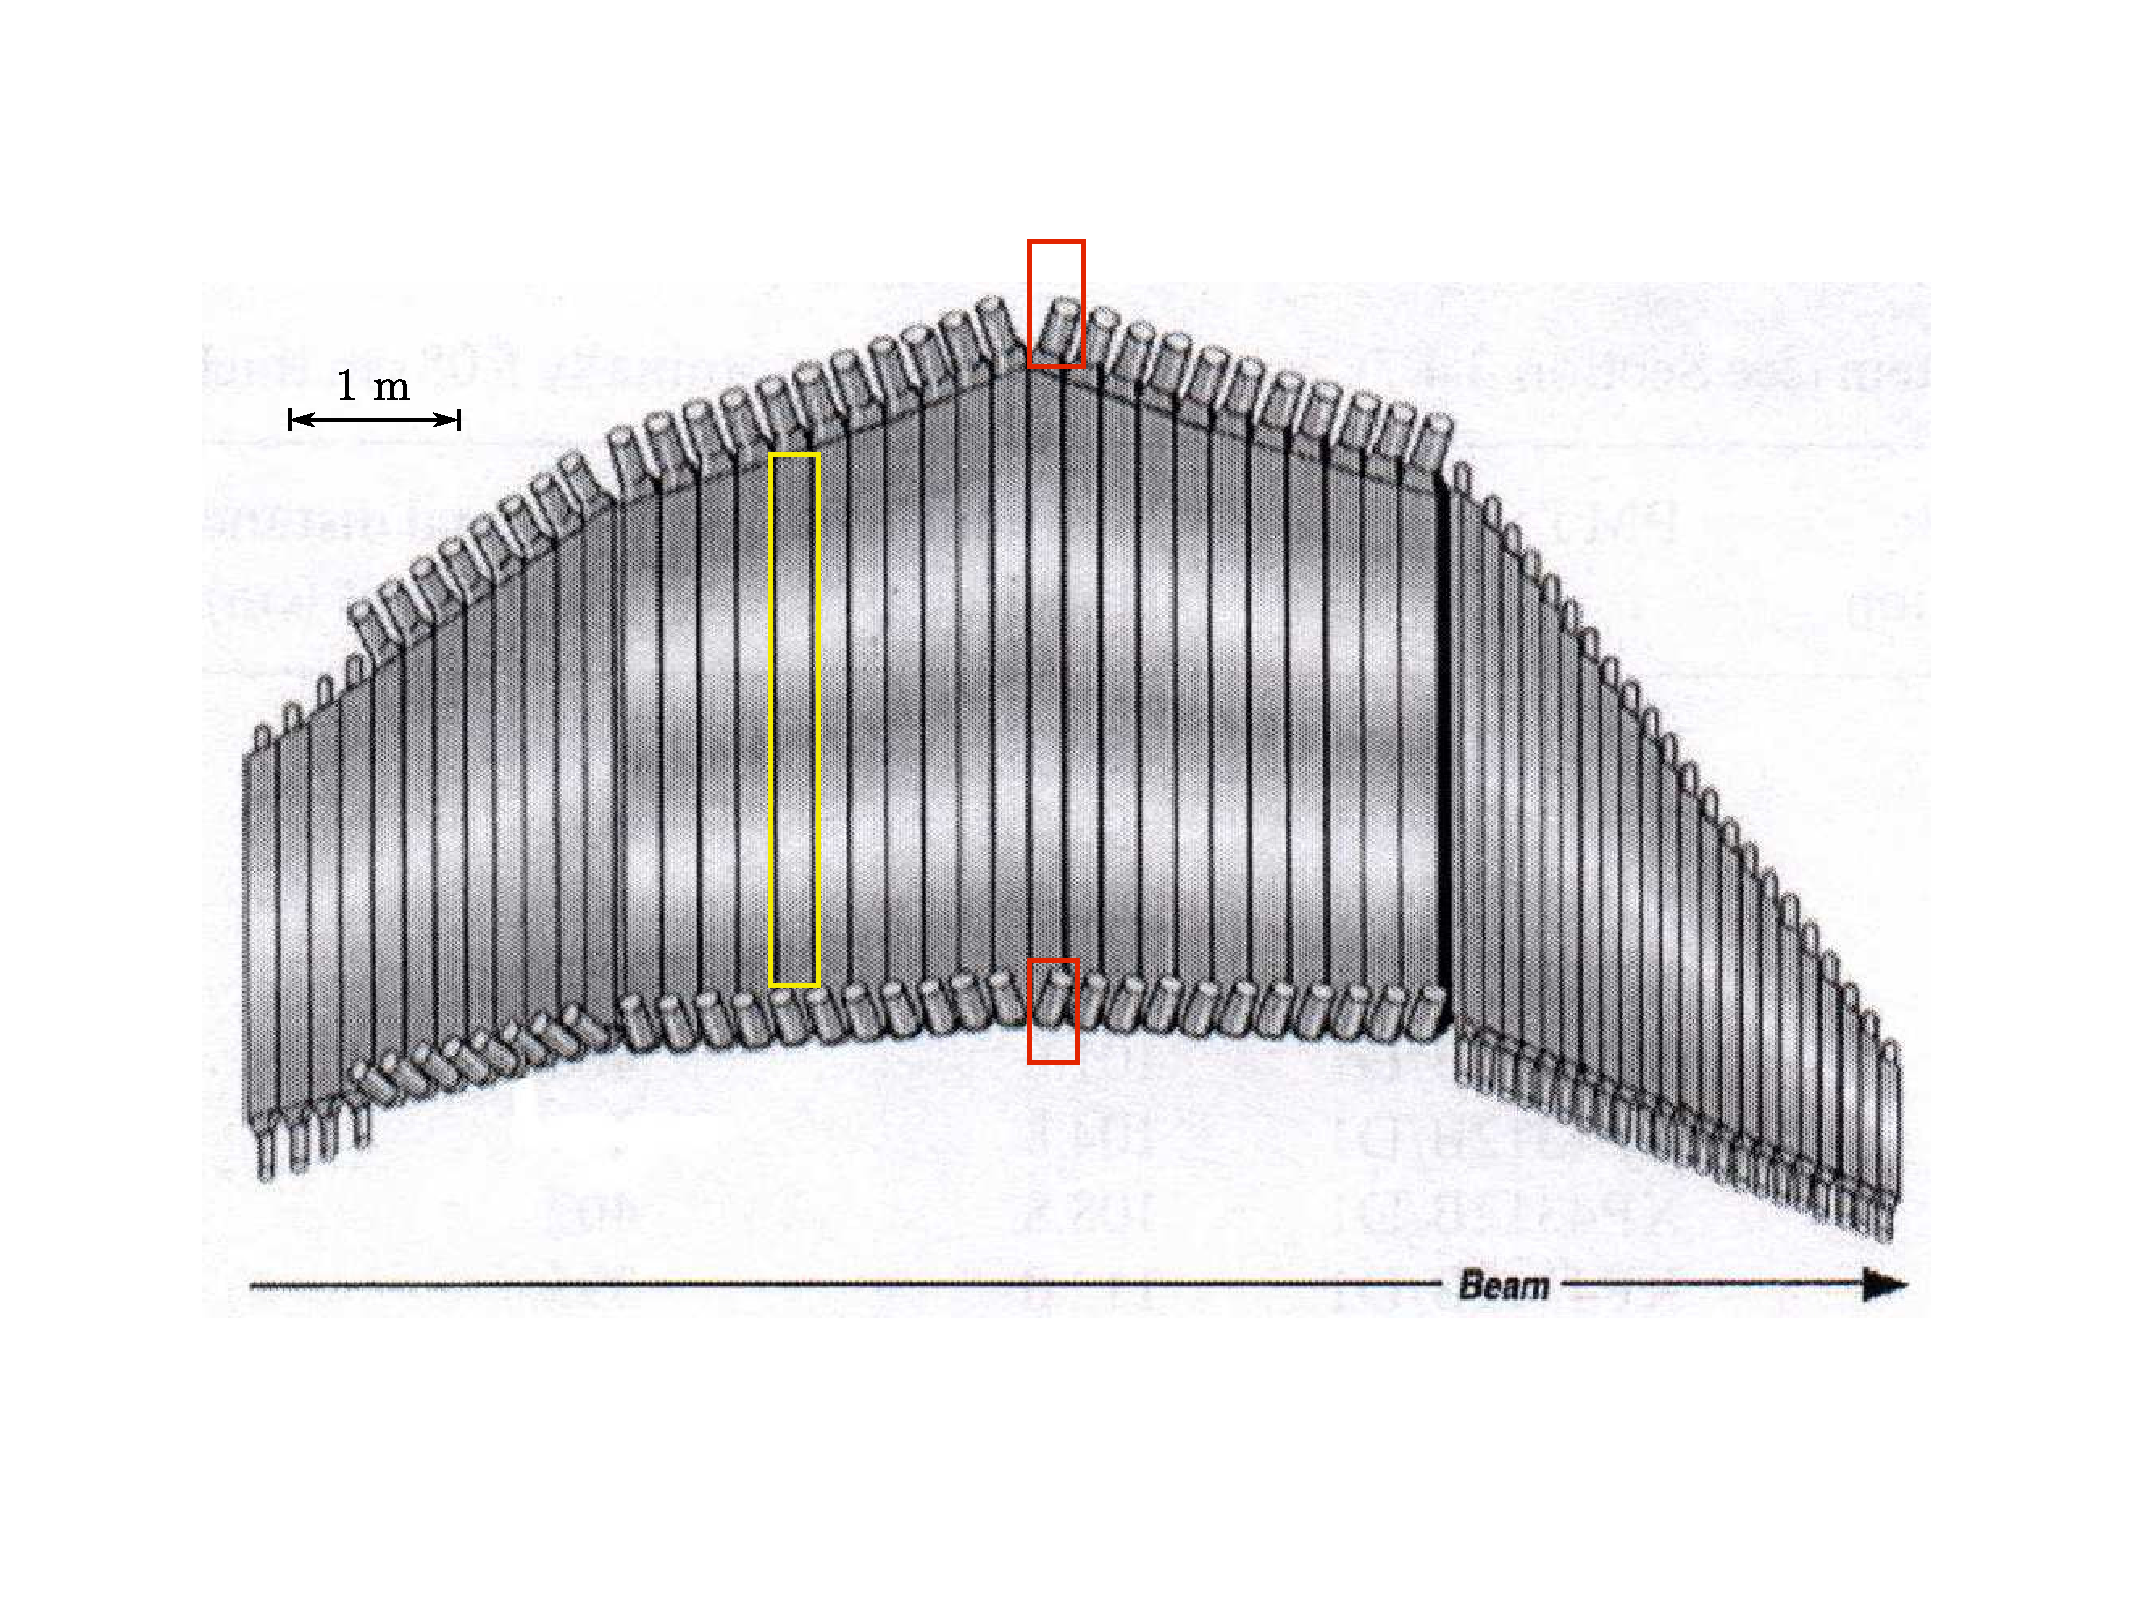
\includegraphics[width=\figwidth]{\figures/hall-b/tof_paddlesII.pdf}
\caption[Diagram of one sector of the time-of-flight (\abbr{TOF}) paddles]{\label{fig:clas.tof.paddles}Diagram of one sector of the time-of-flight (\abbr{TOF}) paddles. There are 57 scintillator paddles covering the entire acceptance region of the drift-chambers for each sector. \abbr{PMT}'s are outlined in red while a scintillator paddle is outlined in yellow.  Image Source:~\cite{clas.tof}}
\end{center}\end{figure}

\FloatBarrier
%\begin{figure}\begin{center}
%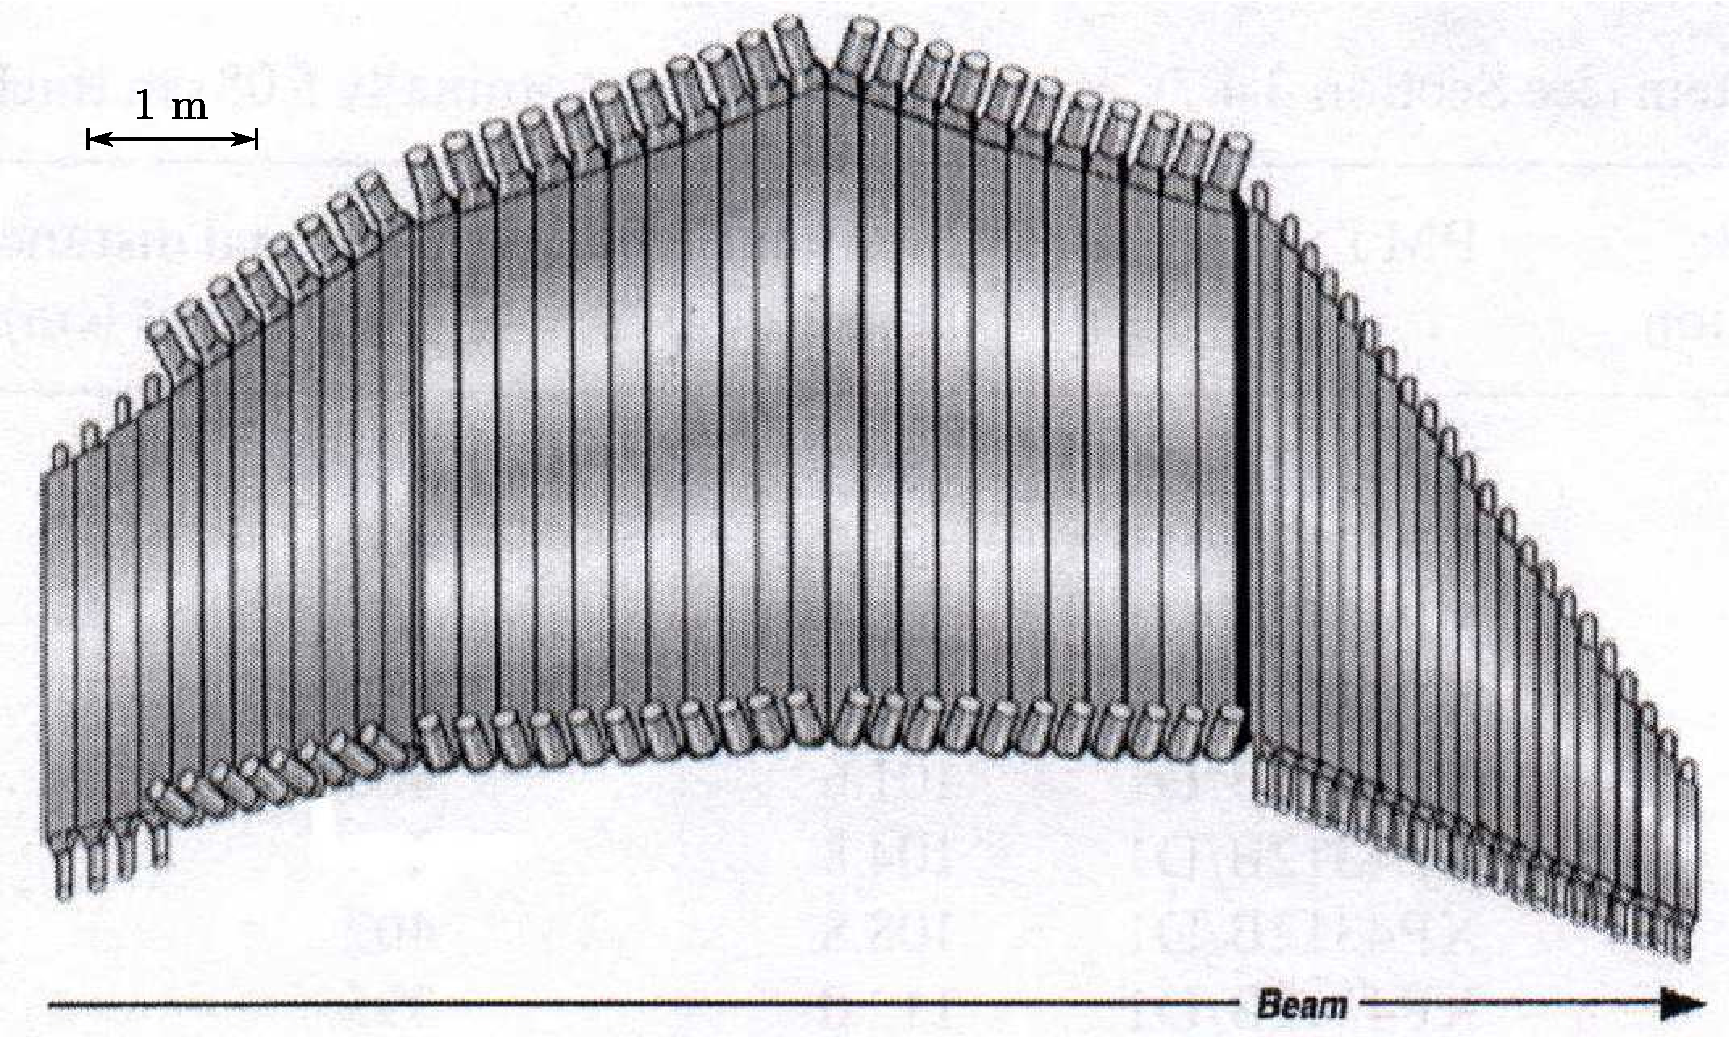
\includegraphics[width=\figwidth]{\figures/hall-b/tof_paddles.pdf}
%\caption[Time-of-Flight Paddles]{\label{fig:clas.tof.paddles}Diagram of one sector of the time-of-flight (\abbr{TOF}) paddles. There are 57 scintillator paddles covering the entire acceptance region of the drift-chambers for each sector.}
%\end{center}\end{figure}
%
%\begin{figure}\begin{center}
%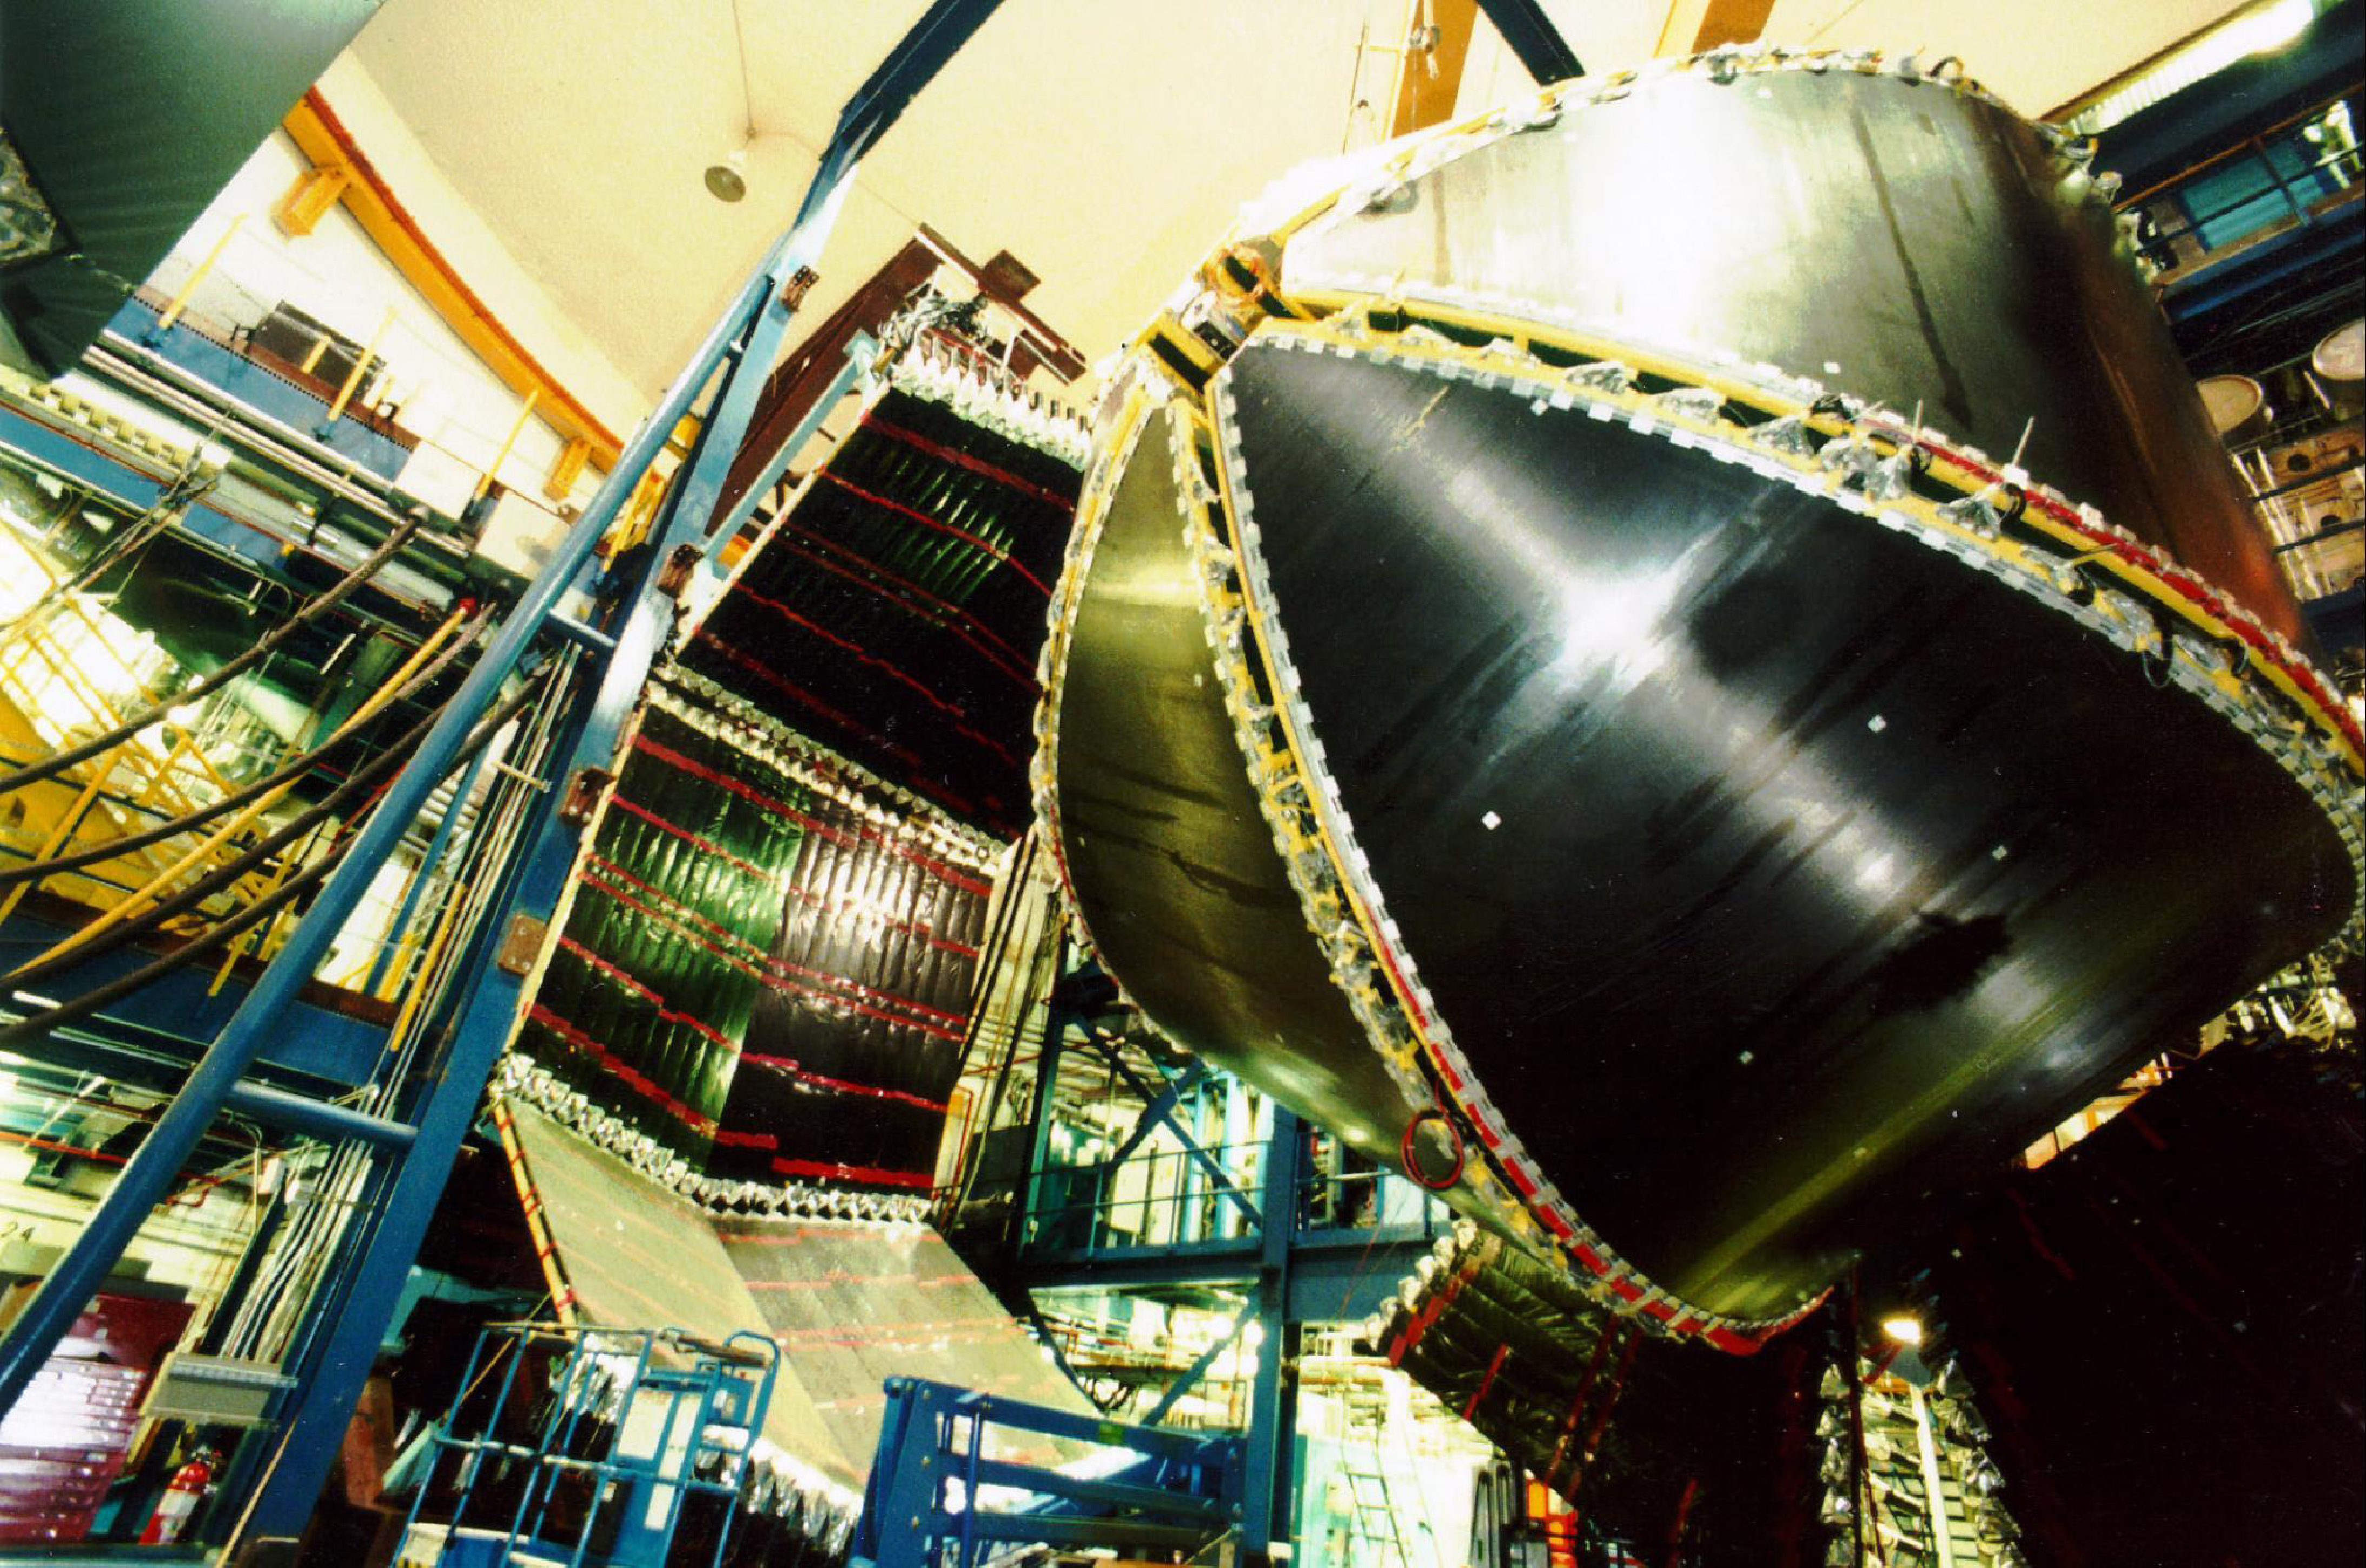
\includegraphics[width=0.8\columnwidth]{\figures/hall-b/clas_detector.pdf}
%\caption[\abbr{CLAS} Detector (photograph)]{\label{fig:clas.photo}The \abbr{CLAS} detector during a maintenance period where the time-of-flight ``shell'' (left) was pulled back from the drift-chambers (\abbr{DC}, right). The beam line enters from the lower right on the other side of the \abbr{DC}. The \abbr{TOF} paddles seen are the two center \emph{panels} shown in Fig.~\ref{fig:clas.tof.paddles} for three of the \abbr{CLAS} sectors.}
%\end{center}\end{figure}
%
%\begin{figure}\begin{center}
%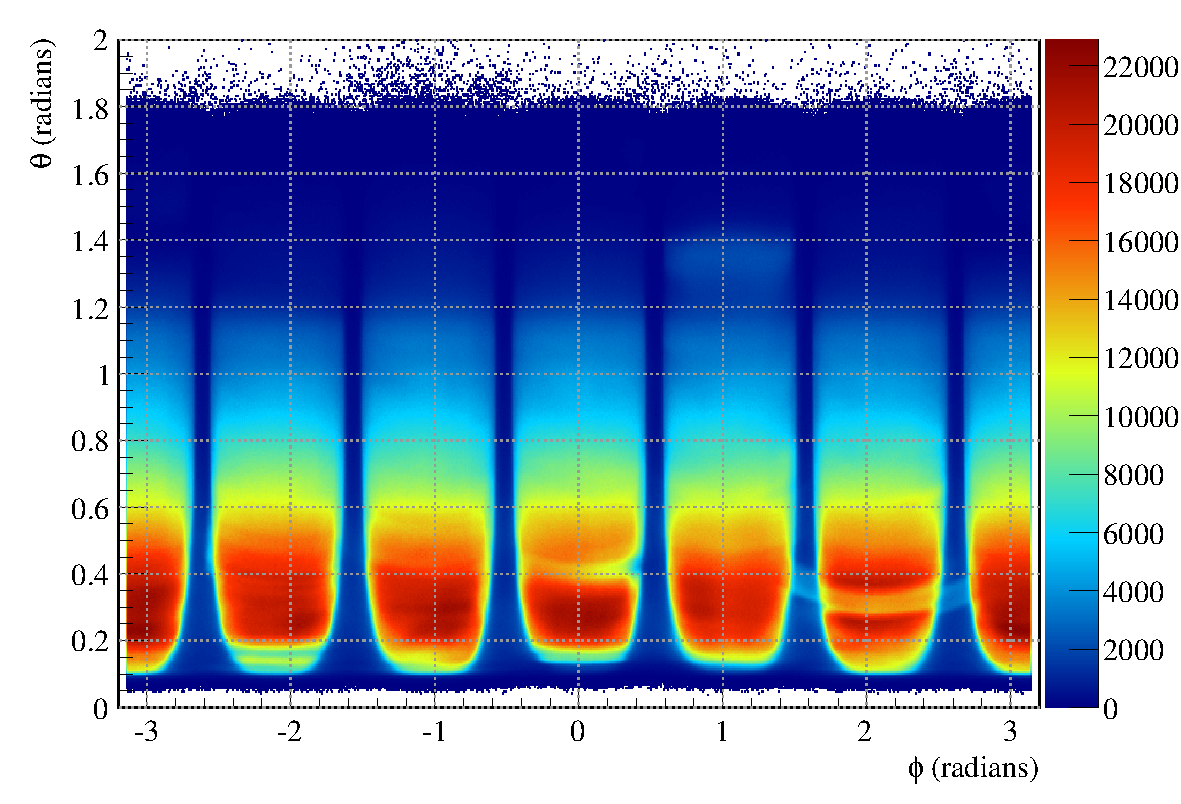
\includegraphics[width=\figwidth]{\figures/reconstruction/coverage_tof.pdf}
%\caption[Time-of-Flight Angular Coverage]{\label{fig:clas.tof.coverage}{\coloronline}Angular coverage in the lab frame of the tracks that had an associated time-of-flight hit. This can be interpreted as the total drift-chamber coverage of the \abbr{CLAS} detector.}
%\end{center}\end{figure}

\section{Electromagnetic Calorimeters}\label{sec:clas.ec}

The calorimetric method implies total absorption of the particle energy in a bulk of material followed by the measurement of the deposited energy. The process usually involves several layers of absorbers and detectors. Depending on the energies and species of particles there are different types of calorimeters. For instance, a 10~GeV muon will require 9~m of Fe or 8~m of Pb to absorb all the energy of the muon. However, a 10~GeV electron will only require 0.2~m of Pb to absorb all the energy.The Electromagnetic Calorimeter was built and used for detection of neutral particles as well as discrimination between electrons and pions.

%\begin{figure}[h!]\begin{center}
%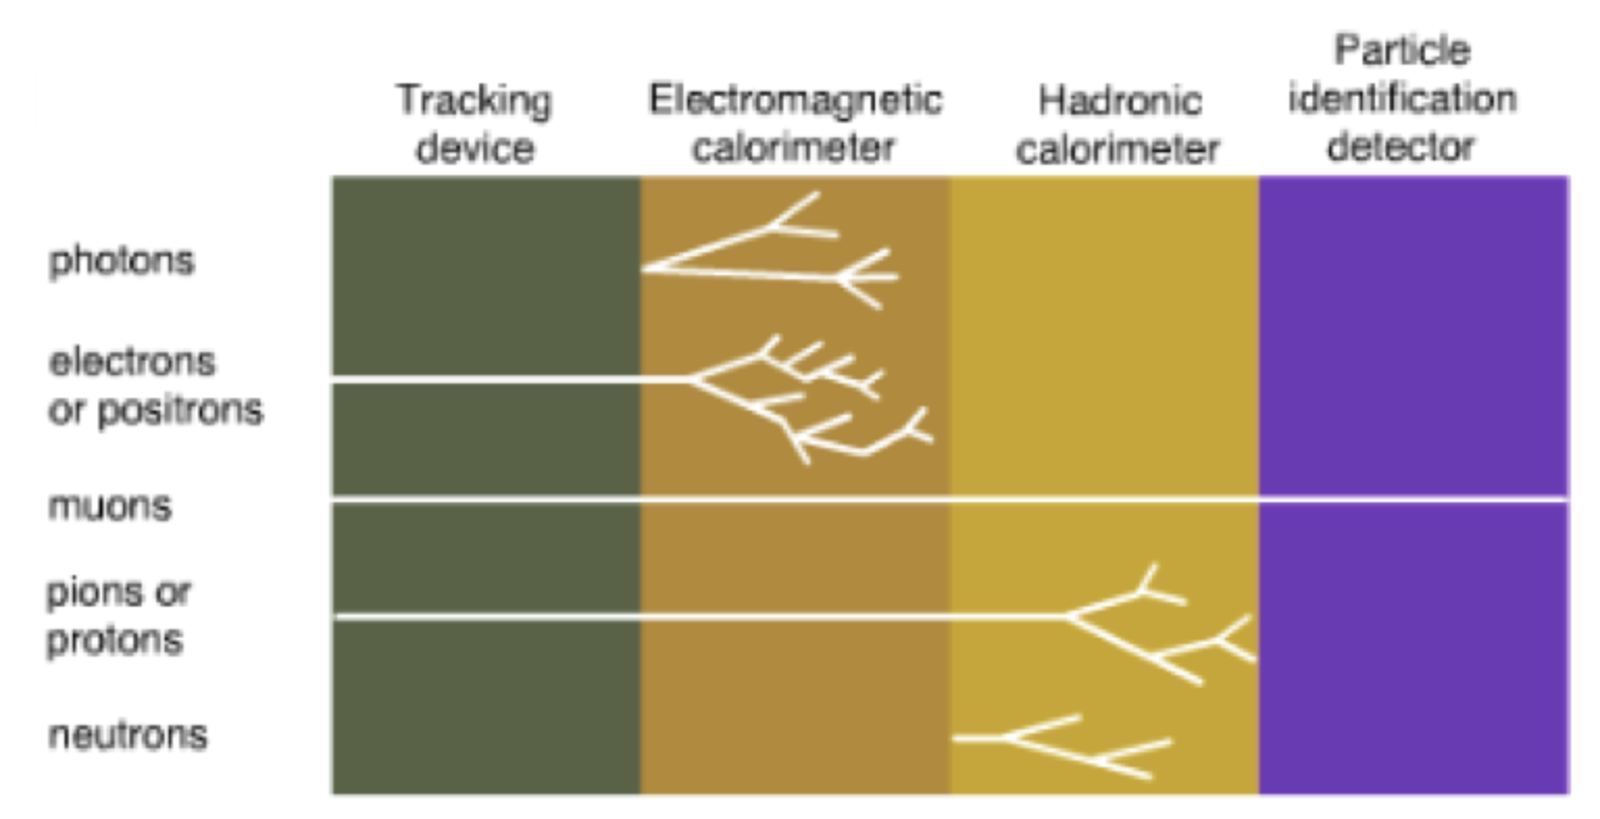
\includegraphics[width=\figwidth,height=\qfigheight]{\figures/hall-b/CCECPLOTS/Calorimetry/detectors.pdf}
%\caption[Types of Calorimeters]{\label{fig:clas.ec.calorim}Type of calorimeter depends on type of hadron detection Image Source:~\cite{C5}}
%\end{center}\end{figure}

\subsection{Electromagnetic Calorimeter}

At energies greater than 100~MeV, electrons lose their energy predominantly by bremsstrahlung while photons lose their energy by electron-positron pair production. The process of bremsstrahlung is electromagnetic radiation produced by the deceleration of an electron when deflected by an atomic nucleus i.e. $\mathrm{e Z \rightarrow Ze\gamma}$. Its cross-section is proportional to $\mathrm{Z^{2}}$ of the material the electron propagates through. The radiation loss of electrons with initial energy $E_0$ can be described as
\begin{align}\label{eq:electron_eloss}
-(\frac{dE}{dx})_{rad} = \frac{E}{X_{0}} \\ \vspace*{10 mm} E(x)=E_{0}e^{\frac{-x}{X_{0}}} 
\end{align}
where $X_{0}$ is the radiation length of the material the electron travels through. The process of pair production, $\gamma Z \rightarrow Ze^{+}e^{-}$ was discussed in Sec.~\ref{sec:intro.conversion}.
%, occurs when a photon with $E_0 > 2 m_e c^2$ converts into an electron and a positron. The cross section for this process can be simplified as
%\begin{equation}\label{pair_crosssection}
%\sigma_{\gamma\rightarrow e^+e^-} =  \frac{A}{N_{A} \rho \lambda_\gamma}  \ ,\ \lambda_\gamma = \frac{9}{7}X_0
%\end{equation}
%where $\lambda$ is also know as the interaction length, or mean free path, $\rho$ is the density of the material, $N_A$ is Avogadro's number and $A$ being the atomic mass of the material. The probability of pair production to occur is solely based on $X_{0}$, the radiation length of the medium and this probability can be expressed as
%\begin{equation}
%\frac{dP}{dx} = \frac{1}{\lambda_\gamma}\exp(\frac{-x}{\lambda_\gamma}) \ .
%\end{equation}

To explain how an Electromagnetic Calorimeter works, assume the absorber for the calorimeter is lead(Pb), Fig \ref{fig:clas.photon_processes} , \ref{fig:clas.electron_processes} depicts the processes for photons and electrons in Pb.
\begin{figure}[h!]\begin{center}
\subfloat[][]{
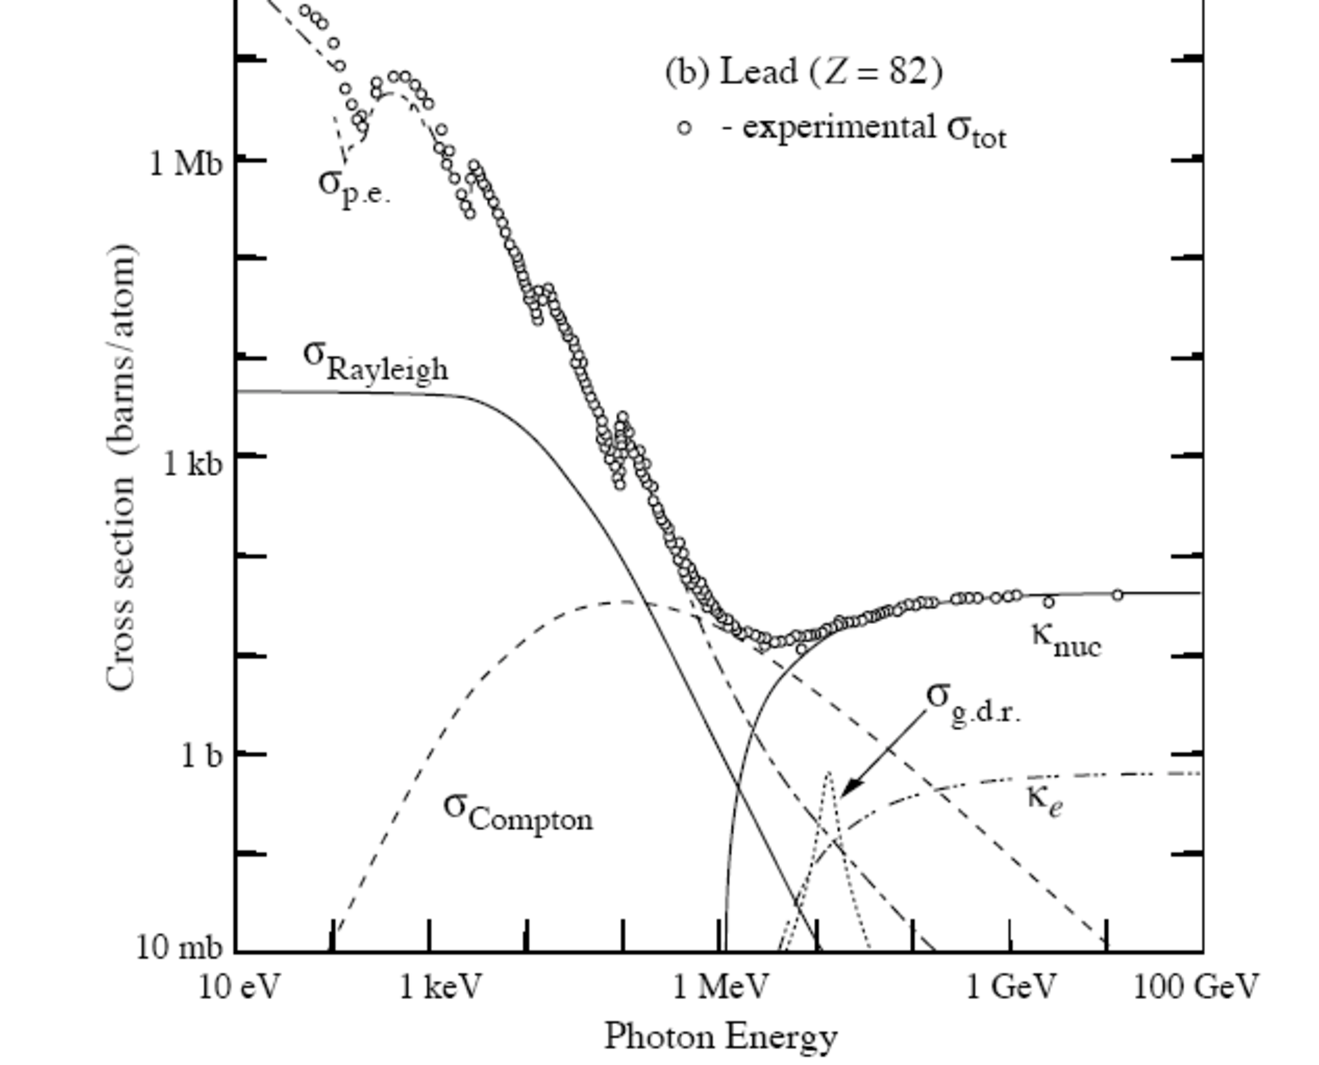
\includegraphics[width=0.45\columnwidth,height=0.5\hfigheight]{\figures/hall-b/CCECPLOTS/Calorimetry/PhotonRadiations.pdf}\label{fig:clas.photon_processes}
}
\subfloat[][]{
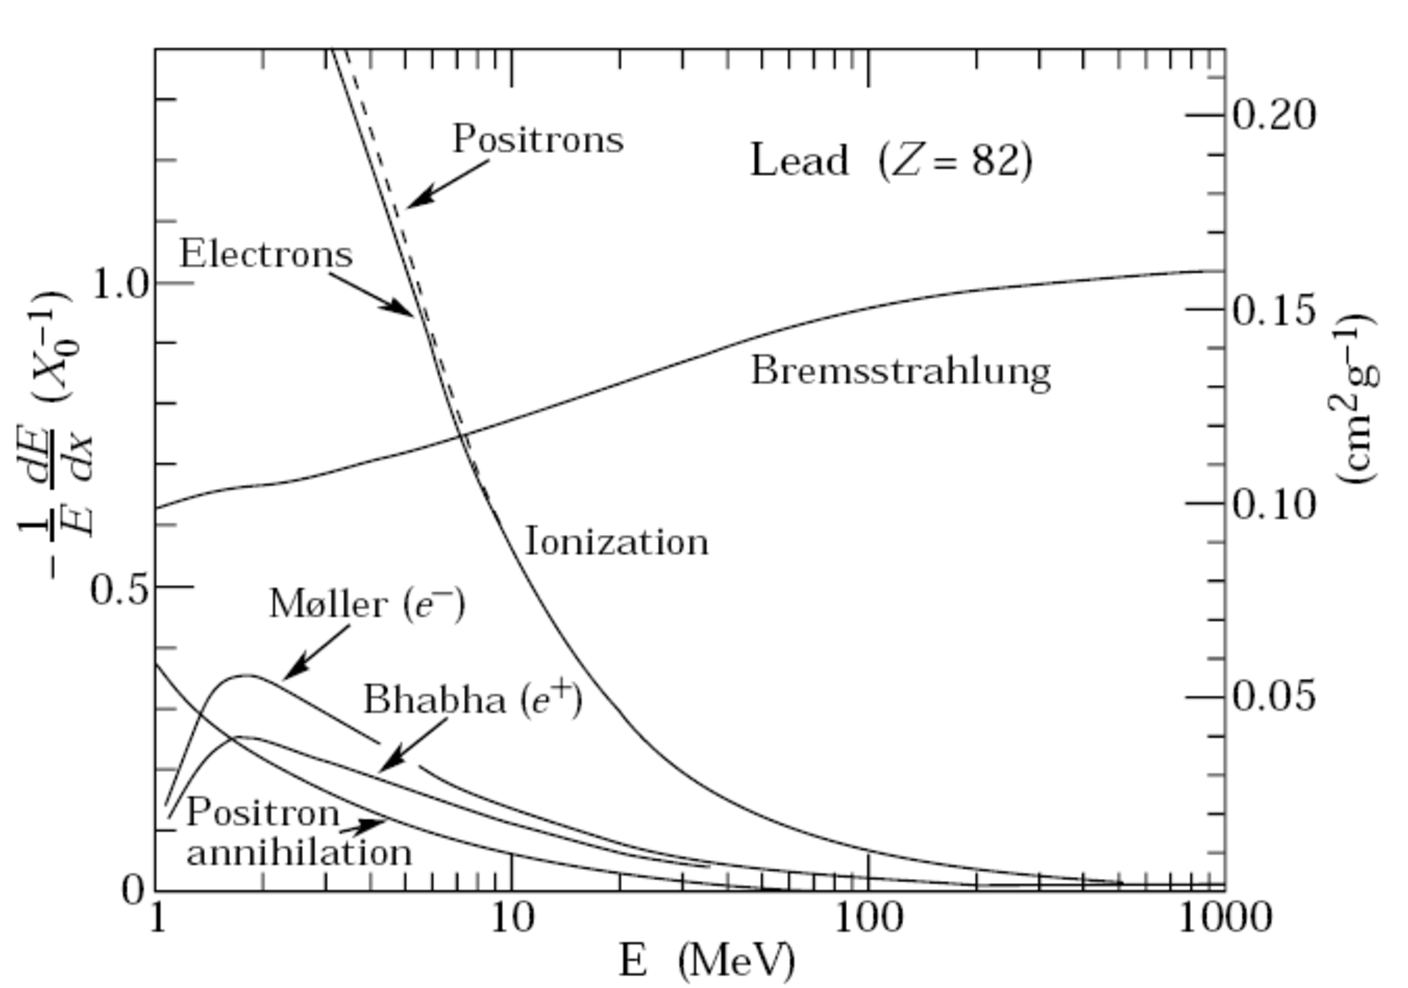
\includegraphics[width=0.45\columnwidth,height=0.5\hfigheight]{\figures/hall-b/CCECPLOTS/Calorimetry/EectronE2.pdf}\label{fig:clas.electron_processes}}
\caption[Photon and Electron processes in \abbr{Pb}]{Photon and Electron processes in \abbr{Pb}~(a) and (b) respectively. Images Source:~\cite{vibe_levels}} 

\end{center}\end{figure}
Lets start with a high energy electron $E_{0}$, after $1 X_{0}$, $\mathrm{1e^{-}}$ and $\mathrm{1 \gamma}$ are produced each with $\frac{E_{0}}{2}$, after $2 X_{0}$, $\mathrm{2e^{-}}$, $\mathrm{1e^{+}}$ and $\mathrm{1 \gamma}$ are produced each with $\frac{E_{0}}{4}$. Therefore after $tX_{0}$, there is a total of 
\begin{equation}
N(t)=2^{t}
\end{equation}
are produced each with
\begin{equation}
E(t) = E_{0}2^{-t}.
\end{equation}
The multiplication of the shower particles continue as long as
\begin{equation}
\frac{E_{0}}{N} > E_{c},
\end{equation}
where $E_{c}$ is the critical energy for showers to propagate,
\begin{align}
E_{c}  = E_{0}2^{-t_{max}} \\
N_{max}=\frac{E_{0}}{E_{c}}
\end{align}

\begin{figure}[h!]\begin{center}
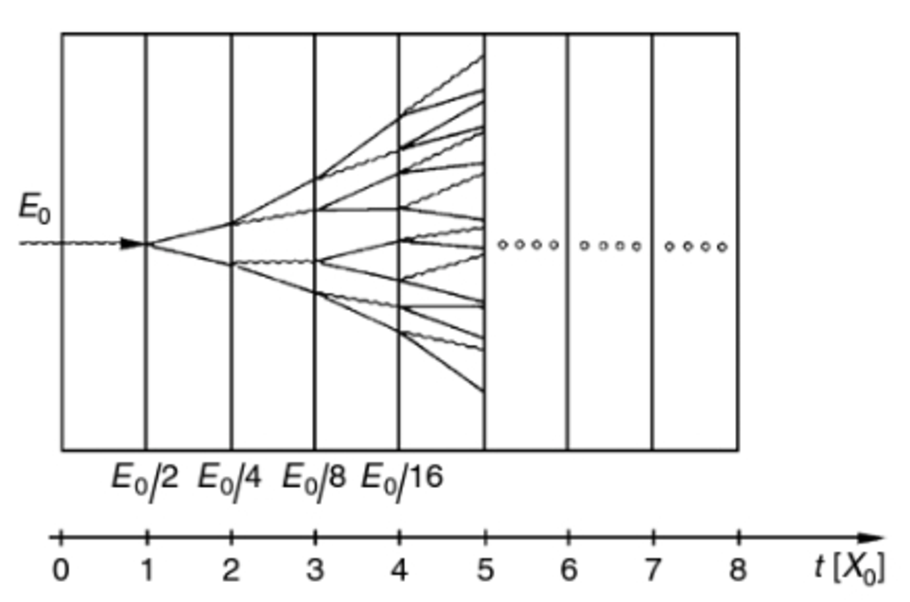
\includegraphics[width=\figwidth,height=\qfigheight]{\figures/hall-b/CCECPLOTS/Calorimetry/cascade.pdf}
\caption[A simple Electromagnetic shower in a calorimeter]{\label{fig:clas.ec.shower}{A simple Electromagnetic shower in a calorimeter} Image Source:~\cite{vibe_levels} }
\end{center}\end{figure}

When a particle falls below critical energy, absorption processes (ionization, Compton and photoelectric) start to dominate the processes for photons and electrons. This leads to
\begin{equation}
t_{max} = \frac{ln(\frac{E_{0}}{E_{c}})}{ln2}.
\end{equation}
At the shower maximum $\mathrm{e^{\pm}}$ will stop within $1X_{0}$ however, photons at critical energy will penetrate further. To absorb 95\% of photons produced in the shower maximum, an additional 7-9$X_{0}$ is necessary. The semi-empirical value for $\mathrm{e^{\pm}}$ $E_c$ in Pb is,
\begin{equation}
E_{c}  \thickapprox \frac{610 MeV}{\mathrm{Z} - 1.24} = 7 MeV 
\end{equation}
which results in $t_{max} \thickapprox 9.7 X_{0}$ for electrons at 6 GeV.

The process shown in Fig~\ref{fig:clas.ec.shower} is a very crude and simple model of an actual shower shown in Fig~\ref{fig:clas.ec.showerII}, but the simple model correctly describes the important features of Electromagnetic Calorimeters
\begin{itemize}
\item The total calorimeter thickness should be more than 10-15~$X_0$ in order to absorb almost all of the energy of an incident photon
\item The position of the shower maximum increases with energy, therefore the thickness of the calorimeter should increase as the logarithm of the energy.
\item If there is energy leakage, it is caused by photons escaping the calorimeter at the sides or at the back.
\end{itemize}

 
\begin{figure}[h!]\begin{center}
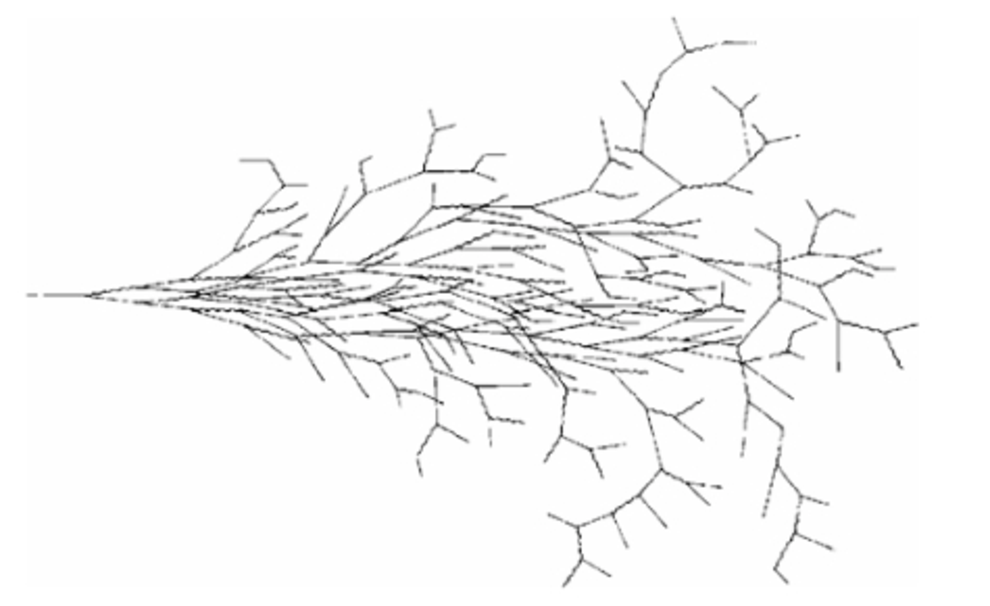
\includegraphics[width=\figwidth,height=\qfigheight]{\figures/hall-b/CCECPLOTS/Calorimetry/cascadeII.pdf}
\caption[A real Electromagnetic shower in a calorimeter]{\label{fig:clas.ec.showerII}{A real Electromagnetic shower in a calorimeter} Image Source:~\cite{vibe_levels} }
\end{center}\end{figure}

\subsection{The \abbr{CLAS} Electromagnetic Calorimeter}

The \abbr{CLAS} electromagnetic calorimeter (\abbr{EC})\cite{clas.ec}, shown in Fig.~\ref{fig:clas} was designed with the following criteria;
\begin{itemize}
\item $\mathrm{e/ \gamma}$ energy resolution $\sigma /E \leq 0.13/ \sqrt{E(GeV)}$
\item Position resolution $\delta r \approx 2cm \ at \ 1GeV$
\item $\mathrm{\pi / e}$ rejection greater than 99\% at $E \geq$1~GeV
\item Fast ($\textless$ 100 ns) total energy sum for the event trigger
\item Mass resolution for 2-photon decays $\delta m / m \leq 0.15$ 
\item Neutron detection efficiency $\textgreater$  50\% for  $E \textgreater$  0.5~GeV
\item Time-of-flight resolution $\approx$ 1 ns
\end{itemize}

The \abbr{EC} consists of alternating layers of Pb (absorber) and scintillator (detector). The lead to scintillator ratio of 0.2, i.e. 40 cm of scintillator, 8 cm of lead (16 $X_{0}$), was chosen so one third of the showering particle's energy is deposited into the scintillator. There are six triangular \abbr{EC} modules, one per sector, each a sandwich constructed of 39 layers. A layer is considered to be 10~mm thick BC412 scintillator followed by 2.2~mm lead. Each scintillator is made of 36 strips parallel to one side and are turned 120$^\circ$ from each other for each $u$, $v$ and $w$ view, 13 layers per view. The \abbr{CLAS} \abbr{EC} is subdivided into two stacks, inner and outer. The inner stack comprises of 8 layers while the outer stack comprises 5 logical layers. Each module contains 36(strips)x3(views)x2(stacks) therefore 216 \abbr{PMT}'s were needed per module, 1296 \abbr{PMT}'s total for \abbr{CLAS} \abbr{EC}, and 8424 scintillator strips. 

\begin{figure}[h!]\begin{center}
\subfloat[][]{
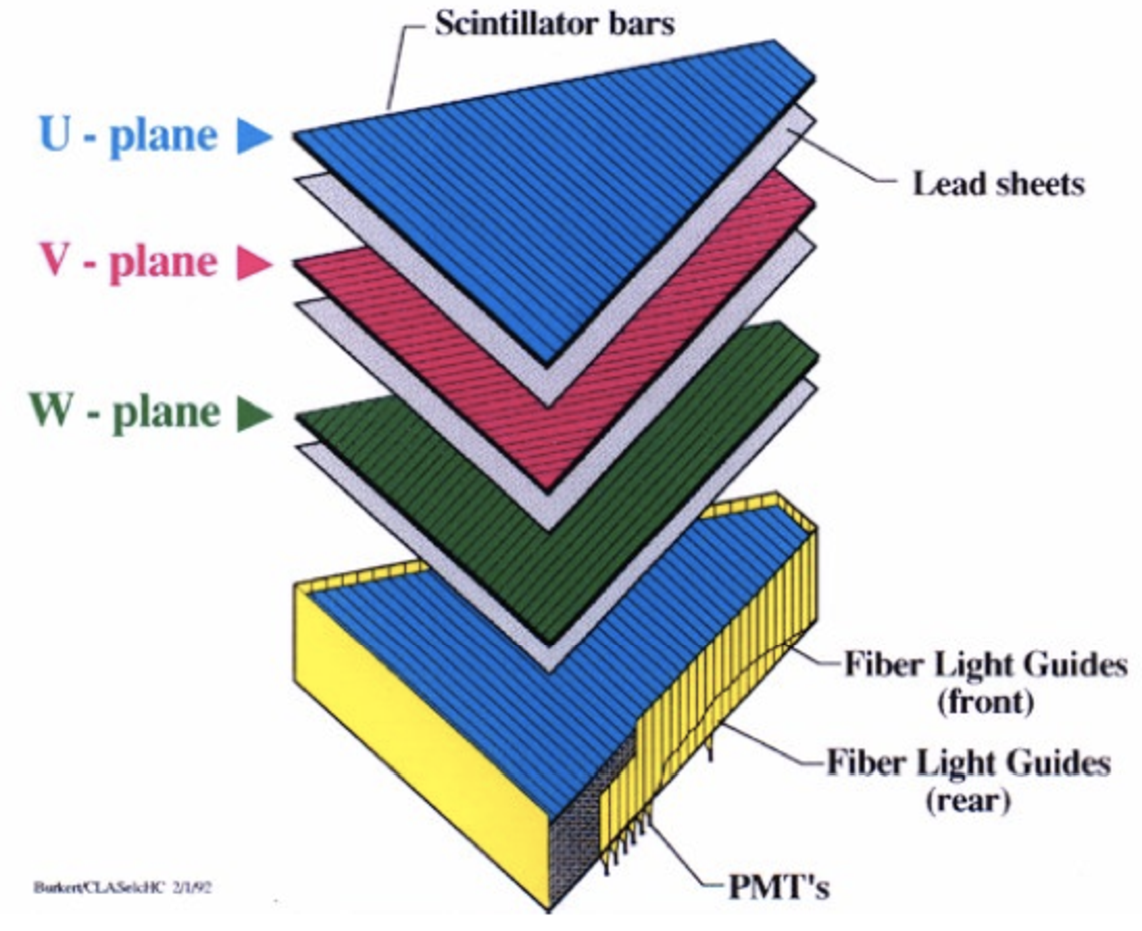
\includegraphics[width=0.8\columnwidth,height=0.75\hfigheight]{\figures/hall-b/CCECPLOTS/Calorimetry/CLASEC.pdf}\label{fig:clas.ec}
}

\subfloat[][]{
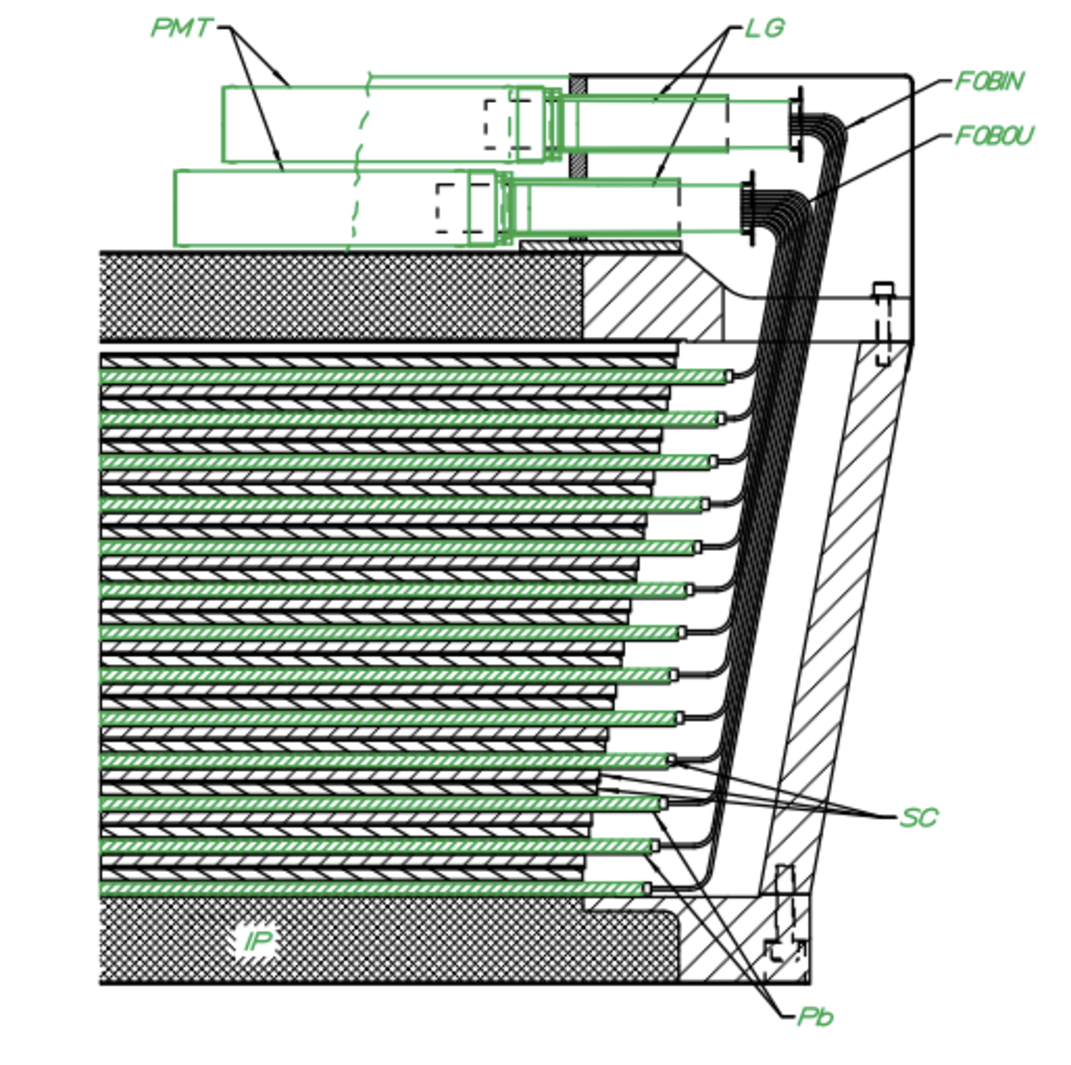
\includegraphics[width=0.8\columnwidth,height=0.75\hfigheight]{\figures/hall-b/CCECPLOTS/Calorimetry/CLASECSIDE.pdf}\label{fig:clas.ec.side}}
\caption[Separated view of one sector of the forward electromagnetic calorimeter (\abbr{EC}) showing the three planes ($u$, $v$, $w$) of scintillator-lead pairs which make up one of the 13 logical layers]{Separated view of one sector of the forward electromagnetic calorimeter (\abbr{EC}) showing the three planes ($u$, $v$, $w$) of scintillator-lead pairs which make up one of the 13 logical layers~(a). Side view of one plane of the forward electromagnetic calorimeter (\abbr{EC}) showing the the 13 logical layers, placement of the \abbr{PMT}'s and light guides~(b). Image Source: \subref{fig:clas.ec}~\cite{clas.ec} , \subref{fig:clas.ec.side}~\cite{clas.ec} respectively.} 

\end{center}\end{figure}

Using the three layers in each logical layer to provide pixel-like information, the transverse shower development for a given particle can be determined. All final-state photons were identified in the \abbr{EC} if no charged tracks have been associated with an energy deposit and also the velocity, $\beta$, of the particle exceeds 0.9c. Particles with $\beta <$~0.9c are neutron candidates.
%The difference in energy deposit between the inner and outer layers provides separation of electrons from pions in the reconstructed data for energies less than 2.8~GeV. For energies greater than 2.8~GeV, identification of pions and electrons are obtained by comparing the energy deposited in the \abbr{EC} with the momentum determined from the \abbr{DC}.



\section{The \g12 Experiment}\label{sec:clas.g12}

briefly explain the need of \g12

\subsection{\g12 Running Condtions}\label{sec:clas.g12.conditions}

explain \g12, use proposals for this

\subsection{G12 Data Acquisition \& Reconstruction }\label{sec:clas.g12.conditions.data}

Explain g12 data retrieval

\subsection{\g12 Corrections}\label{sec:clas.g12.corrections}

lets write about the beam corrections that were needed because of hysteresis and also the efficiency corrections needed for ''normalization" 
%
%Three \abbr{CLAS} analysis proposals (\abbr{04-005}\cite{clas.proposal.hyclas}, \abbr{04-017}\cite{clas.proposal.superg} and \abbr{08-003}\cite{clas.proposal.pion}) defined the experimental and theoretical basis for the \g12 running period. \label{sec:clas.hyclas}The \abbr{04-005} experiment, \emph{Search for New Forms of Hadronic Matter in Photoproduction}, also called \abbr{HyCLAS}, had a meson spectroscopy focus with multiple charged particle final states such as
%\begin{eqnarray}
%    \gamma \p & \rightarrow & \p \pi^+ \pi^- \pi^0, \\
%    \gamma \p & \rightarrow & \n \pi^+ \pi^+ \pi^-, \\
%    \gamma \p & \rightarrow & \p \Kp \Km \eta, \\
%    \gamma \p & \rightarrow & \n \Kp \Kp \pi^-, \\
%    \gamma \p & \rightarrow & \Delta^{++} \eta \pi^-, \\
%    \gamma \p & \rightarrow & \p \p \bar{\p}.
%\end{eqnarray}
%The physics involved with \abbr{HyCLAS} required the configuration of \abbr{CLAS} to provide the largest acceptance for these multiple particle final states. Phase-space generated events of $\mathrm{\gamma p \rightarrow p \pi^+ \pi^- \pi^0}$ were simulated (see page~30 of \cite{clas.proposal.hyclas}) with the $t$-slope obtained from the \textit{g6c} experiment. The primary requirement for the greatest acceptance of such events was to have the target up-stream (see Sec.~\ref{sec:clas.tgt}) of the normal position at the ``center'' of \abbr{CLAS}. This target placement gave better acceptance for particles close to the beam-line but sacrificed large momentum-transfer events where the final state particles were more than about 70$^\circ$ away from the beam-line.
%
%\label{sec:clas.superg}The \abbr{04-017} experiment, \emph{Study of Pentaquark States in Photoproduction off Protons}, also called \abbr{Super-G}, was founded on a search for the $\Theta^+$ and $\Xi^{--}_{5}$, so-called \emph{penta-quarks}, as well as a study of the ``conventional'' $\Xi$ spectrum (see page~16 of \cite{clas.proposal.superg}.) This analysis is part of the latter topic. The running requirements were similar to that of \abbr{HyCLAS} with the need for a higher energy beam. An examination of the ground state $\Xi^-$ reaction:
%\[
%    \mathrm{\gamma p \rightarrow \Xi^- K^+ K^+},
%\]
%provides a starting point for this analysis. The threshold energy of the incident photon ($E_\gamma$) is given by
%\begin{equation}
%    E_{\gamma} = \frac{m_{\Xi}^2 + 4 m_{\mathrm{K}}^2 + 4 m_{\rule{0pt}{1.4ex}\Xi} m_{\rule{0pt}{1.4ex}\mathrm{K}} - m_{\p}^2}{2 m_{\p}},
%\label{eqn:xi.threshold}
%\end{equation}
%where $m_{\rule{0px}{1.4ex}\Xi}$ is the mass of the $\Xi$, $m_{\rule{0px}{1.4ex}\mathrm{K}}$ is the mass of the K$^{+}$, and $m_{\p}$ is the proton (target particle) mass. For the ground state $\Xi(1320)$ which has a mass of 1.322~GeV, the threshold energy $E_\gamma$ is 2.4 GeV. Since the beam
%(photon) and the target (proton) are both known quantities, we can measure the two kaons and calculate the $\Xi^-$ through ``missing mass'' which is discussed in detail in Chapter~\ref{sec:analysis}. There is a minimum transverse momentum the final state particles must have to be measured by \abbr{CLAS}, otherwise they would travel right down the beam line. Therefore, in order to detect the two kaons with \abbr{CLAS}, a photon energy approximately 0.5~GeV above threshold is required. This corresponds to 2.9~GeV in the reaction for the ground state $\Xi(1320)$.
%
%The third proposal, \abbr{08-003}, titled \emph{The $\gamma \p \rightarrow \pi^+ \n$ Single Charged Pion Photoproduction}, was approved just before the \g12 run period started. This was added onto \g12 as part of the physics to be done with the data collected. It required a single track trigger (see Sec.~\ref{sec:data.trig} on page~\pageref{sec:data.trig}) and lower current. This configuration allowed the data from these special runs to be included in analyses of the ``production'' \g12 data set.
%
%At the beginning of \g12 run, approval came for purchasing gas for the \v{C}erenkov subsystem of \abbr{CLAS}; see Sec.~\ref{sec:clas.cc}. The \v{C}erenkov counters were filled and turned on two weeks into the running period enabling the separation of electons from pions. As a result, a whole new set of leptonic physics became available in what was already a very rich data set.

\begin{flushleft}
\begin{flushleft}

\end{flushleft}
\end{flushleft}\chapter{Particle Reconstruction and Analysis}\label{sec:analysis}

This chapter will explore the methods and techniques used for particle reconstruction and analysis. There were 2 packages of algorithms used to perform particle identification, while only one was used for the analysis part. The algorithms used for particle identification were codes compiled in the \emph{``clas6-trunk''} under the package \abbr{CLASEVENT}. \abbr{CLASEVENT} is a C++, class-based package written primarily by Dennis Weygand for the purpose of analyzing the output of the reconstruction program that was discussed in Sec.~\ref{sec:data.cook}. For this analysis, \abbr{CLASEVENT} was utilized to skim the reconstructed data and output the data into \abbr{ROOT} format for later evaluation. 

The second set of algorithms used to perform this analysis were written primarily by the author, except for the algorithms pertaining to the kinematic fitter. The second set of algorithms were built off of the \abbr{ROOT} platform. The kinematic fitter algorithms were written by Dustin Keller and the procedure of kinematic fitting is discussed in Sec.~\ref{sec:analysis.fitting}. 
\section{Data Reduction and Event Selection}\label{sec:analysis.event}
\subsection{Excluded Runs}\label{sec:analysis.excluded}

For this analysis 165 production runs, all single-prong runs and all special calibration runs were excluded. Table~\ref{tab:excluded_runs} contains a list of the runs that are excluded along with the reason of exclusion.

\input{tables/Excluded_runs}


\subsection{\label{sec:analysis.event_selection}Event Selection}

During the skimming process, \abbr{CLASEVENT} employs several corrections to the data that are necessary to analyze the data. Such corrections are ``energy-loss'' and ``tagger-sag'' correction which are discussed in Sec.~\ref{sec:analysis.corrections.eloss} and Sec.~\ref{sec:analysis.corrections.beam} respectively. 

The skim performed on the \abbr{BOS} files included the criteria of Table~\ref{tab:skim.requirements} using the \abbr{PART} reconstruction scheme. There is another particle reconstruction scheme, \abbr{EVNT}. However this method was first reported unreliable for \g12 by the author of this manuscript and then later confirmed by various other users.
\input{tables/skim_requirements}
Pions were skimmed initially and then re-identified as leptons by changing the mass of the pion. This method is sufficient when the decaying particle's mass, i.e. $m_{\pi^0}$, is less than that of pions. If the event satisfied the requirements listed in Table~\ref{tab:skim.requirements}, then all \abbr{TOF}, \abbr{ST}, momentum and vertex information was outputted as well as \abbr{CC} and \abbr{EC} information for the $\pi^{\pm}$ particles to be used to identify leptons, as discussed in Sec~\ref{sec:analysis.pid}. To reduce the size of the data set, a cut was placed on the total missing mass of $\gamma p \to p \pi^{+} \pi^{-}$ to be less than 275~MeV. This cut was broad enough to not interfere with \piz selection from single \piz production i.e. $\gamma p \to p \pi^{0}$ when assigned the pion the lighter mass of a electron/positron. This broad cut also does not interfere with \piz production from light meson decay, i.e $\gamma p \to p \omega \to p \pi^{+} \pi^{-} \pi^{0}$.


\subsection{Beam Photon Identification}\label{sec:analysis.beam}

As described in Sec.~\ref{sec:analysis.excluded}, only runs in which the beam current was 60-65~nA were used. This high current incident on the radiator can create multiple tagger hits within the time gate of the trigger. To determine which beam photon interacted with the target creating the event, a tagger time best matching the average \abbr{ST} time is chosen to be the time of the interacting photon that created the triggered event.

Due to the 2.004~ns \abbr{CEBAF} beam bunching spacing, there are possibilities in which a beam bunch will contain multiple bremsstrahlung photons that are indistinguishable in timing, within 2.004~ns, that satisfy the best tagger time. Figs~\ref{fig:beam.timing} and~\ref{fig:beam.timingII} show that $\simeq$ 86\% of events have a single in-time tagger-\abbr{ST} coincidence, $\simeq$ 11.5\% of events have two in-time tagger-\abbr{ST} coincidences, $\simeq$ 2\% of events have three in-time tagger-\abbr{ST} coincidences and $<$ .5\% of events have have more than three in-time tagger-\abbr{ST} coincidences. For the events in which there are multiple photons within the 2.004~ns window that are in time with the \abbr{ST}, the best photon is chosen at random with no preference to the energies of each photon. This method of random choice allows for a 7\% background increase due to the mismatching of the photon The 7\% is due to randomly choosing the incorrect photon $\frac{1}{2}$ of the 14\%. 

\begin{figure}[h!]\begin{center}
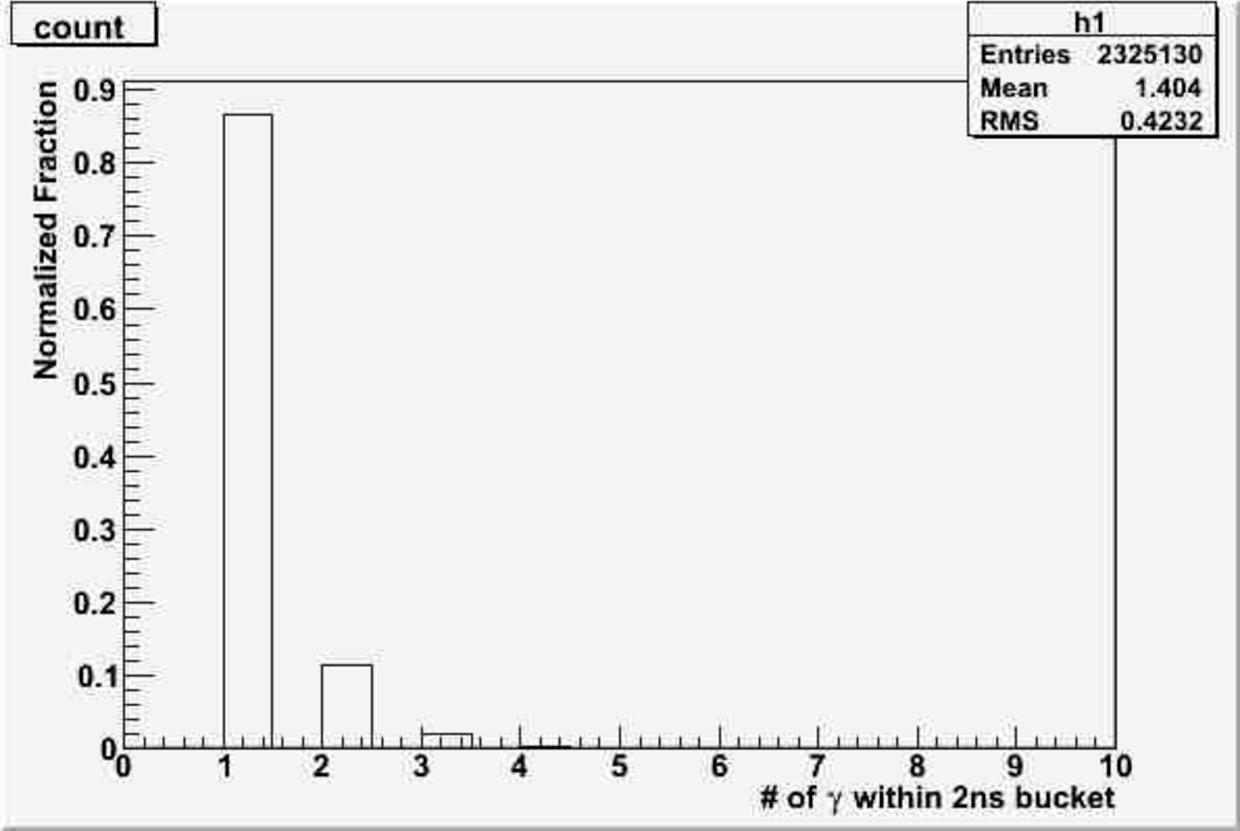
\includegraphics[width=\figwidth,height=0.75\hfigheight]{\figures/analysis/photon_timing/Photoncount1.pdf}
\caption[Probability of single and multiple photons within the \abbr{CEBAF} timing window of 2.004~ns]{\label{fig:beam.timing}Probability of single and multiple photons within the \abbr{CEBAF} timing window of 2.004~ns.}
\end{center}\end{figure}

\begin{figure}[h!]\begin{center}
\includegraphics[width=\figwidth,height=0.75\hfigheight]{\figures/analysis/photon_timing/Photoncount.pdf}
\caption[Probability of multiple photons within the \abbr{CEBAF} timing window of 2.004~ns]{\label{fig:beam.timingII}Probability of multiple photons within the \abbr{CEBAF} timing window of 2.004~ns.}
\end{center}\end{figure}

\FloatBarrier
\subsection{Particle Identification}\label{sec:analysis.pid}

Lepton identification was based on conservation of mass. Once the data is skimmed according to Table~\ref{tab:skim.requirements}, all particles that were $\pi^+$, $\pi^-$, unknown with $q^+$ or unknown with $q^-$ were tentatively assigned to be electrons or positrons based on their charge. This meant that the mass term of the particle's 4-vector was set to be the mass of an electron instead of that of a pion. This technique works because the mass of the \piz (0.135~GeV) is less than the mass of $\pi^+$ or $\pi^-$ (0.139~GeV) and by laws of conservation of energy-momentum, a lighter particle cannot decay into heavier particle's.
%To explain this effect, lets consider a particle A decaying into daughters B and C.
%\begin{align}
%A\rightarrow B+C
%\end{align}
%In the rest frame of A the 4-momentum transforms to  
%\begin{align}
%P_A\rightarrow (0,M_A), \nonumber \\
%P_B\rightarrow (\overline{P}_B,E_B), \nonumber \\
%P_C\rightarrow (\overline{P}_C,E_C),
%\end{align}
%where $\overline{P}_B$ and $\overline{P}_C$ are the 3-momentum of particles B and C respectively. Using conservation of 4-momentum and the property $P_i^2 = m_i^2$, $E_C$ can be calculated as;
%\begin{align}\label{eq:piz.kinematics}
%P_B^2 = (P_A - P_C)^2 \nonumber \\
%M_B^2 = P_A^2 + P_C^2 - 2P_A\cdot P_C \nonumber \\
%M_B^2 = M_A^2 + M_C^2 - 2M_AE_C \nonumber \\
%E_C = \frac{M_A^2 + M_C^2 - M_B^2}{2M_A}.
%\end{align}
%For the case in which particle A is a \piz and the particles B and C are electron and positron which have equal mass eq.~\ref{eq:piz.kinematics} simplifies to 
%\begin{align}\label{eq:piz.decay}
%E_C = \frac{M_{\pi^0}^2}{2}.
%\end{align}
%The same procedure can be applied for particle B which would yield the same result as eq.~\ref{eq:piz.decay} with the interchange of the index $C\leftrightarrow B$. From eq.~\ref{eq:piz.decay} it can be seen that because 
%\begin{align}\label{eq:piz.energy}
%E_{C,B} = \sqrt{M_{C,B}^2 + \overline{P}_{C,B}^2} \nonumber
%\end{align}
%that
%\begin{align}
%M_{C,B} <  \frac{M_{\pi^0}^2}{2}, \nonumber
%\end{align}
%therefore \piz cannot decay into particles of heavier mass.

For particles with higher masses that can decay into two-pions  or into \epem, such as $\eta,\ \omega$, etc., the \abbr{CC} and \abbr{EC} provide a $\frac{e^+e^-}{\pi^+\pi^-}$ rejection factor of $\approx 10^6$. The method to achieve this rejection factor was developed by Mike Wood and is based on using various cuts placed on the \abbr{CC} and \abbr{EC} measured quantities. This method was not used in this analysis, the $\gamma p \to  p \pi^0 \to p e^+e^-\gamma$ reaction provides insight into the validity of the method. The Mike Wood method of $\frac{e^+e^-}{\pi^+\pi^-}$ rejection factor is discussed in~\cite{clas.g12.note}.   


%\section{General Features of Lepton Data in \g12}\label{sec:analysis.Lepton.general}

Electron and positron energy deposition while propagating through a material was briefly explained in Sec.~\ref{sec:clas.cc} and ~\ref{sec:clas.ec}. To identify electrons and positrons properly in \abbr{CLAS}, quantities obtained from the \abbr{CC} and \abbr{EC} are used to reject charged pions. The \abbr{CC} collects the number of photo-electrons caused by Cherenkov radiation and the \abbr{EC} records the energy deposition of electrons/positrons as well as photons. A previous \abbr{CLAS} experiment \emph{g7} analyzed the properties of medium modifications from the decay of vector mesons through the leptonic decay channel. This experiment derived a set of cits for identifying electron/positrons pairs in \abbr{CLAS} by employing specific cuts to the number of photo-electrons (\abbr{NPE}) detected in the \abbr{CC}, a match in azimuthal angle $\phi$ from a charged track in the \abbr{DC} to the $\phi$ of the \abbr{CC}, as well as comparing the momentum of the charged track to the energy deposited in the \abbr{EC}. These cuts can be found in Table~\ref{tab:ISLEP_cuts}.  
\input{tables/islep}
To validate the \emph{g7} electron/positron \abbr{PID} scheme for \g12, a comparison of  the \abbr{CC} and \abbr{EC} quantities was performed for all charged tracks \abbr{CC}/\abbr{EC} hit signatures and while selecting events from \piz decay. To separate the \piz events from the $\pi^{+}\pi^{-}$ events, all charged pions were assigned the mass of electrons and cuts were placed on the missing energy of $\gamma p \rightarrow p e^+ e^-$ as well as a cut on the missing mass squared of $\gamma p \rightarrow p$, values found in Table~\ref{tab:lep_cuts}. A graphical depiction of the cuts applied to separate \piz events from the $\pi^{+}\pi^{-}$ events is seen in Fig.~\ref{fig:islep.cuts}.
\input{tables/lepPIDcuts} 
The values of the threshold momentum are calculated from empirical studies and are based upon calculations using the momentum obtained from the \abbr{DC }$p$ under the following criteria;
\begin{align}
\mathrm{p_{thres}^{low}} = \alpha p *(p+EC_{P\_LO})/p \nonumber \\
\mathrm{p_{thres}^{high}} = \alpha p *(p+EC_{P\_HIGH})/p \nonumber
\end{align}
where $EC_{P\_LO} = -0.3$, $EC_{P\_HIGH} = 0.5$ and  
\begin{align}
\alpha p =
\begin{cases}
.23*p + .071p^2 - .032p^3, & p<1.0 \mathrm{~GeV} \\
0.272p, & p>1.0 \mathrm{~GeV} \\
\end{cases}\nonumber
\end{align}


\begin{figure}[h!]\begin{center}
\includegraphics[width=\figwidth,height=\hfigheight]{\figures/analysis/LEP_FEATURES/Lepfeature_cuts.pdf}
\caption[Cuts Applied to Isolate \piz and $\pi^{+}\pi^{-}$ for \abbr{PID} Validation]{\label{fig:islep.cuts}Plot of missing mass squared of off proton (horizontal) vs. missing energy of proton e$^+$e$^-$ (vertical). The red dashed vertical line depicts the $\pi^{+}\pi^{-}$ threshold mass cut while the horizontal red dashed line represents the missing energy cut-off used to sepertate $\pi^{+}\pi^{-}$ from \piz.}
\end{center}\end{figure}

\subsubsection{\abbr{CC} Comparison}

The \abbr{NPE} measured by the \abbr{CC} for all positron/electron (e$^+$/e$^-$) candidates can be seen in Fig~\ref{fig:islep.CC}. The sharp decline prior to 2.5 \abbr{NPE} is due to photo-electrons created by electron/positrons, pions traveling through the \abbr{CC} or pions producing delta-electrons which pass through the \abbr{CC}. Delta-electrons are created as an effect of the ionization of gases that could be present when the pion travels through the \abbr{DC}. These types of electrons are typically lower in momentum than the electrons obtained from particle decays in \abbr{CLAS} and thus according to eq.~\ref{eq:cc.NPE} should emit less \abbr{NPE} per unit length.

Through mass conservation, as discussed in Sec.~\ref{sec:analysis.pid}, the particles in the \piz events must be e$^+$/e$^-$ pairs. In comparison to fig.~\ref{fig:islep.CC}, fig.~\ref{fig:islep.CC1} plots the \abbr{NPE} measured by the \abbr{CC} for all e$^+$/e$^-$ pairs for \piz events selected as shown in fig.~\ref{fig:islep.cuts}. It can be seen that the sharp decline prior to \abbr{NPE} = 2.5 is reduced leaving mostly electrons or positrons signatures in the \abbr{CC} concluding that the \emph{g7} \abbr{CC} \abbr{NPE} cut is valid for identifying e$^+$/e$^-$ pairs while rejecting $\pi^+$/$\pi^-$ pairs.
 
%
\begin{figure}[h!]\begin{center}
\includegraphics[width=\figwidth,height=\hfigheight]{\figures/analysis/LEP_FEATURES/CC_nPE.pdf}
\caption[Number of Photo-electrons Measured by \abbr{CC} for All e$^-$ and e$^+$ Candidates]{\label{fig:islep.CC}Plot of \abbr{NPE} measured by \abbr{CLAS} \abbr{CC} subsystem for positron/electron candidates top/bottom respectively. The dashed dotted vertical line depicts the cut applied if using the \emph{g7} lepton \abbr{PID} scheme.}
\end{center}\end{figure}

\begin{figure}[h!]\begin{center}
\includegraphics[width=\figwidth,height=\hfigheight]{\figures/analysis/LEP_FEATURES/CC_NPEcut.pdf}
\caption[Number of Photo-electrons Measured by \abbr{CC} for \piz Events]{\label{fig:islep.CC1}Plot of \abbr{NPE} measured by \abbr{CLAS} \abbr{CC} subsystem when selecting \piz events seen in Fig~\ref{fig:islep.cuts}, positron/electron candidates top/bottom respectively.}
\end{center}\end{figure}
\FloatBarrier
\subsubsection{\abbr{EC} Comparison}
%EC
%
%e-
%

Similarly to the \abbr{CC} comparison, figures~\ref{fig:islep.pimEClow},~\ref{fig:islep.pimEChigh},~\ref{fig:islep.pipEClow},~\ref{fig:islep.pipEChigh} depict the  p$\mathrm{_{thres}^{low}}$ and  p$\mathrm{_{thres}^{low}}$ cuts listed in  Table~\ref{tab:ISLEP_cuts} for the q$^-$ and q$^+$ tracks respectively. After \piz event selection, seen in figures~\ref{fig:islep.pimEC},~\ref{fig:islep.pimECcut} ,~\ref{fig:islep.pipEC} ,~\ref{fig:islep.pipECcut}, the bulk of e$^+$/e$^-$ events reside within the region of the cut acceptance therefore it is evident that the \emph{g7} \abbr{EC} cuts are valid for identifying e$^+$/e$^-$ pairs. The following four plots are for electron($e^-$) \abbr{PID} validation of the \emph{g7} \abbr{EC} cuts described in Table~\ref{tab:ISLEP_cuts}.
%
\begin{figure}[h!]\begin{center}
\includegraphics[width=\figwidth,height=0.7\hfigheight]{\figures/analysis/LEP_FEATURES/Pim_EClow.pdf}
\caption[\abbr{EC} Deposited Energy Comparison to Lower Threshold Track Momentum for q$^-$ Tracks]{\label{fig:islep.pimEClow}Plot of energy deposited measured by \abbr{EC} vs. track momentum p$\mathrm{_{thres}^{low}}$ for negative charged tracks. The red region depicts the cut that would reject events in the \emph{g7} lepton \abbr{EC} \abbr{PID} scheme.}
\end{center}\end{figure}

\begin{figure}[h!]\begin{center}
\includegraphics[width=\figwidth,height=0.7\hfigheight]{\figures/analysis/LEP_FEATURES/Pim_EChigh.pdf}
\caption[\abbr{EC} Deposited Energy Comparison to Upper Threshold Track Momentum for q$^-$ Tracks]{\label{fig:islep.pimEChigh}Plot of energy deposited measured by \abbr{EC} vs. track momentum p$\mathrm{_{thres}^{high}}$ for negative charged tracks. The red region depicts the cut that would reject events in the \emph{g7} lepton \abbr{EC} \abbr{PID} scheme.}
\end{center}\end{figure}


\begin{figure}[h!]\begin{center}
\includegraphics[width=\figwidth,height=0.7\hfigheight]{\figures/analysis/LEP_FEATURES/Pim_EClowcut.pdf}
\caption[\abbr{EC} Deposited Energy Comparison to Track Momentum for e$^-$ Candidates]{\label{fig:islep.pimEC}Plot of energy deposited measured by \abbr{EC} vs. track momentum p$\mathrm{_{thres}^{low}}$ for electrons from \piz events without the \emph{g7} lepton \abbr{EC} \abbr{PID} scheme applied. The red region depicts the cut that would reject events in the \emph{g7} lepton \abbr{EC} \abbr{PID} scheme.}
\end{center}\end{figure}

\begin{figure}[h!]\begin{center}
\includegraphics[width=\figwidth,height=0.7\hfigheight]{\figures/analysis/LEP_FEATURES/Pim_EChighcut.pdf}
\caption[\abbr{EC} Deposited Energy Comparison to Track Momentum for e$^-$ from \piz Events]{\label{fig:islep.pimECcut}Plot of energy deposited measured by \abbr{EC} vs. track momentum p$\mathrm{_{thres}^{high}}$ for electrons from \piz events without the \emph{g7} lepton \abbr{EC} \abbr{PID} scheme applied. The red region depicts the cut that would reject events in the \emph{g7} lepton \abbr{EC} \abbr{PID} scheme.}
\end{center}\end{figure}
\FloatBarrier
The following four plots are for positron($e^+$) \abbr{PID} validation of the \emph{g7} \abbr{EC}
cuts described in Table~\ref{tab:ISLEP_cuts}.
%
%
%e+
%
%
\begin{figure}[h!]\begin{center}
\includegraphics[width=\figwidth,height=0.7\hfigheight]{\figures/analysis/LEP_FEATURES/Pip_EClow.pdf}
\caption[\abbr{EC} Deposited Energy Comparison to Lower Threshold Track Momentum for q$^+$ Tracks]{\label{fig:islep.pipEClow}Plot of energy deposited measured by \abbr{EC} vs. track momentum p$\mathrm{_{thres}^{low}}$ for positive charged tracks. The red region depicts the cut that would reject events in the \emph{g7} lepton \abbr{EC} \abbr{PID} scheme.}
\end{center}\end{figure}

\begin{figure}[h!]\begin{center}
\includegraphics[width=\figwidth,height=0.7\hfigheight]{\figures/analysis/LEP_FEATURES/Pip_EChigh.pdf}
\caption[\abbr{EC} Deposited Energy Comparison to Upper Threshold Track Momentum for q$^+$ Tracks]{\label{fig:islep.pipEChigh}Plot of energy deposited measured by \abbr{EC} vs. track momentum p$\mathrm{_{thres}^{high}}$ for positive charged tracks. The red region depicts the cut that would reject events in the \emph{g7} lepton \abbr{EC} \abbr{PID} scheme.}
\end{center}\end{figure}

\begin{figure}[h!]\begin{center}
\includegraphics[width=\figwidth,height=0.7\hfigheight]{\figures/analysis/LEP_FEATURES/Pip_EClowcut.pdf}
\caption[\abbr{EC} Deposited Energy Comparison to Track Momentum for e$^+$ Candidates]{\label{fig:islep.pipEC}Plot of energy deposited measured by \abbr{EC} vs. track momentum p$\mathrm{_{thres}^{low}}$ for positrons from \piz events without the \emph{g7} lepton \abbr{EC} \abbr{PID} scheme applied. The red region depicts the cut that would reject events in the \emph{g7} lepton \abbr{EC} \abbr{PID} scheme.}
\end{center}\end{figure}

\begin{figure}[h!]\begin{center}
\includegraphics[width=\figwidth,height=0.7\hfigheight]{\figures/analysis/LEP_FEATURES/Pip_EChighcut.pdf}
\caption[\abbr{EC} Deposited Energy Comparison to Track Momentum for e$^+$ from \piz Events]{\label{fig:islep.pipECcut}Plot of energy deposited measured by \abbr{EC} vs. track momentum p$\mathrm{_{thres}^{high}}$ for positrons from \piz events without the \emph{g7} lepton \abbr{EC} \abbr{PID} scheme applied. The red region depicts the cut that would reject events in the \emph{g7} lepton \abbr{EC} \abbr{PID} scheme.}
\end{center}\end{figure}
%


\FloatBarrier



\section{\g12 Corrections}\label{sec:analysis.corrections}
There were three corrections that were implemented onto the \g12 data set. The first correction was applied to the tagger subsystem due to a magnetic field problem that affected only the \g12 experiment. The second correction corrects for the ``energy-loss'' of a particle through matter. These corrections are discussed further in the proceeding subsections. The third correction was the tagger sag correction that was handled in the tagger calibration.
\subsection{Energy Loss}\label{sec:analysis.corrections.eloss}

Since tracking began after the particle had already traversed through the target and \abbr{ST}, the measured momentum was decreased by the ``energy-loss'' the particle underwent before entering the Region 1 \abbr{DC}. This ``energy-loss' is due to charged particles losing their energy through atomic excitation and ionization while traveling through materials in the \abbr{CLAS} detector. The effect of ``energy-loss'', in \abbr{CLAS}, is only indicative to all charged particles. However, using the Bethe-Bloch equation:
\begin{align}
\frac{dE}{dx} \sim \frac{\ln \gamma}{\beta^2} \ ,
\end{align}
where $\gamma$ and $\beta$ have their usual meanings, it is seen that for electrons with $\beta \approx 1$ lose less energy than protons. Therefore ``energy-loss" corrections are not applied to electrons or positrons. For those charged particles that are subject to ``energy-loss'', such as the proton for this analysis, corrections were made to account for energy lost in the target material ($\ell H_2$), kapton target walls, the beam pipe, the start counter and the air between the start counter and the Region 1 \abbr{DC}. The corrections were applied by the eloss software package written by Eugene Pasyuk for the CLAS detector~\cite{clas.eloss} as an add-on to the \abbr{CLASEVENT} software package.

\subsection{Beam Corrections}\label{sec:analysis.corrections.beam}
Initially, missing masses computed for \g12 were systematically low. It was realized while investigating the issue that the low missing mass depended on run number and varied by as much as 10~MeV. The run dependent missing mass showed a constant low mass (run$<$56550) followed by a higher mass which remained constant (56500$<$run$<$56920) until another increase in mass (run$>$56920). To analyze and correct for the problem, two reactions were chosen to select missing protons and neutrons. The first reaction;
\begin{equation}
\gamma p \rightarrow \pi^+ \pi^- p \label{eq:beam.cortopology}
\end{equation}
was used to derive the correction, while the second reaction;
\begin{align}
\gamma p \rightarrow \pi^+ \pi^+ \pi^- (n)  \label{eq:beam.checktopology}
\end{align}
was chosen to verify the corrections. The reaction of Eq.~\ref{eq:beam.cortopology} was used to derive the correction because all three particles can be detected. Thus
\begin{align}
(P_{\gamma} + P_{target} - (P_{\pi^+} + P_{\pi^-}))^2 = P^2_{p} = m_p^2 \,
\end{align}
where $P_{\gamma}$, $P_{target}$,$P_{\pi^{\pm}}$ and $P_{p}$ are the 4-vectors of the incident photon, target, $\pi^{\pm}$ and proton respectively and $m_p$ is the mass of the proton.
We selected events for the correction with one \abbr{CLAS} \abbr{PID} $\pi^+$, one \abbr{CLAS} \abbr{PID} $\pi^-$, one \abbr{CLAS} \abbr{PID} proton and nothing else. Exclusive cuts were then placed by requiring the missing energy, $M_E(\gamma p \rightarrow p \pi^+ \pi^-) < 0.025$~GeV and the missing mass squared of $M_x^2(\gamma p \rightarrow p \pi^+ \pi^-) < 0.015$~GeV$^2$. These cuts assure that the selected evetns did not have a undetected $pi^0$,
since the mass squared of \piz $= 0.0182$~GeV$^2$.

The first step chosen was to verify whether the ``energy-loss'' correction was causing the discrepancy,. This can be seen in Figs.~\ref{fig:beamcor.p_mass},~\ref{fig:beamcor.n_mass}. It was concluded that the ``energy-loss'' correction was not the problem. From Fig.~\ref{fig:beamcor.p_mass}, two runs were chosen, 56515 and 57130, in which the difference in the missing mass was $\approx$10~MeV. Inspecting the invariant mass, $M(\pi^+\pi^-)$, Fig~\ref{fig:beamcor.k_mass}, for runs 56515 and 57130 revealed only a mass deviation of $\approx$1.4~MeV. This implies that the problem  is caused by the photon beam energy.


\begin{figure}[h!]\begin{center}
\includegraphics[width=\figwidth,height=0.75\hfigheight]{\figures/analysis/beam_correction/P_mass_issue.pdf}
\caption[Plot of \g12 run number vs. undetected proton mass with and without the ``energy-loss'' applied]{\label{fig:beamcor.p_mass}Plot of \g12 run number vs. undetected proton mass with and without the ``energy-loss'' applied. }
\end{center}\end{figure}

\begin{figure}[h!]\begin{center}
\includegraphics[width=\figwidth,height=0.75\hfigheight]{\figures/analysis/beam_correction/N_mass_issue.pdf}
\caption[Plot of \g12 run number vs. undetected neutron mass with and without the ``energy-loss'' applied]{\label{fig:beamcor.n_mass}Plot of \g12 run number vs. undetected neutron mass with and without the ``energy-loss'' applied. The red data points labeled ``mss" are data taken directly from tape. Image Source:~\cite{bookwalter}}
  \end{center}\end{figure}
  
  \begin{figure}[h!]\begin{center}
  \includegraphics[width=\figwidth,height=0.7\hfigheight]{\figures/analysis/beam_correction/Kaon_mass.pdf}
  \caption[Plot of $\pi^+ \pi^-$ mass for runs 56515 and 57130]{\label{fig:beamcor.k_mass}Plot of $\pi^+ \pi^-$ mass for runs 56515 and 57130. $m_{K_0}$ = 0.4976 GeV/c$^2$.}
  \end{center}\end{figure}
  % % %
  \FloatBarrier
  Several tagger quantities were analyzed. The tagger magnet current was apparently constant (see Fig.~\ref{fig:tag.magnet.epics}) but had been turned off around run=56920 (May 12, 2008). When the tagger magnet was turned on, the current was set to its previous setting. The tagger magnet current was recorded by the accelerator group shown in Fig.~\ref{fig:tag.magnet.arne}, it was also stable throughout the running of \g12. The beam current was also stable (see Fig.~\ref{fig:beamcurrents})
  
  %Now that it is known that the photon beam energy is the cause of the issue, it must be known the cause of the photon beam error. Several quantities that the tagger subsystem are subjected to were analyzed, first being the tagger magnet current which, according to the \abbr{EPICS} Fig~\ref{fig:tag.magnet.epics}, remain constant
  %but showed that around run = 56920 (May 12, 2008) the tagger magnet was shut-off. The tagger magnet shut-off was done because work had to be done in the hall, however after the tagger magnet was turned on, the current was set to its previous setting. A further investigation into the tagger magnet was performed by private communication with the accelerator group chief Arne Freyberger, Fig~\ref{fig:tag.magnet.arne} shows the data the accelerator group had for the tagger magnet which confirms that the tagger magnet current was stable throughout the running of \g12. The next beam quantity analyzed was the beam current delivered by \abbr{CEBAF}, again through private communication with the accelerator group chief Arne Freyberger it is shown in Fig.~\ref{fig:beamcurrents} that the electron beam current remained constant throughout the \g12 experiment.
  
  \begin{figure}[h!]\begin{center}
  \includegraphics[width=\figwidth,height=0.7\hfigheight]{\figures/analysis/beam_correction/600px-Hystersis_smokingGun.pdf}
  \caption[Tagger magnet current according to \abbr{EPICS}]{\label{fig:tag.magnet.epics}Tagger magnet current according to \abbr{EPICS}}
  \end{center}\end{figure}
  
  \begin{figure}[h!]\begin{center}
  \includegraphics[width=\figwidth,height=0.7\hfigheight]{\figures/analysis/beam_correction/tagger_current_arne.pdf}
  \caption[Tagger magnet current according to accelerator group via \abbr{EPICS}]{\label{fig:tag.magnet.arne} Tagger magnet current according to accelerator group via \abbr{EPICS}}
  \end{center}\end{figure}
  
  \begin{figure}[h!]\begin{center}
  \includegraphics[width=\figwidth,height=0.7\hfigheight]{\figures/analysis/beam_correction/beam_currentsII.pdf}
  \caption[Electron beam current delivered to hall \desg{B}(red) and hall \desg{C} (green) according to the accelerator group during \g12]{\label{fig:beamcurrents}Electron beam current delivered to hall \desg{B}(red) and hall \desg{C} (green) according to the accelerator group during \g12. The green line overlays the red line except during the time around April, 03, 2008.}
  \end{center}\end{figure}
  
  The next quantity investigated was the positioning of the beam spot on the tagger dump. This quantity was used in place of the tagger magnetic field strength because hall \desg{B} does not measure the tagger magnetic field strength. However since the radius of curvature of a charged particle is inversely proportional to the magnetic field this quantity is suitable.
  \begin{equation}\label{eq:motioninmagII}
  p = qrB \ (\mathrm{if}\ \vec{p} \perp \vec{B} )
  \end{equation}
  The y-position of the tagger beam spot on the dump jumps on or about May 12, 2008 (see Fig.~\ref{fig:tagdump}). The change in y-position can only be due to the magnetic field changing. The phenomena in magnetism that allows for a steady current but a change in magnetic field is known as hysteresis (see Fig.~\ref{fig:hyst}).
    \begin{figure}[h!]\begin{center}
  \includegraphics[width=\figwidth,height=0.7\hfigheight]{\figures/analysis/beam_correction/600px-Tagger-dump-y.pdf}
  \caption[Tagger dump beam spot y-position according to \abbr{EPICS}]{\label{fig:tagdump}Tagger dump beam spot y-position according to \abbr{EPICS}}
  \end{center}\end{figure}
  
  \begin{figure}[h!]\begin{center}
  \includegraphics[width=\figwidth,height=0.7\hfigheight]{\figures/analysis/beam_correction/hysteresis_keynote.pdf}
  \caption[Plot depicting magnetic field strength vs. magnet current showing the process of hysteresis]{\label{fig:hyst}Plot depicting magnetic field strength vs. magnet current showing the process of hysteresis. For a current of strength I, there could exist many magnetic fields of strength B.}
  \end{center}\end{figure}
  \FloatBarrier
  It appeared that the \g12 missing mass fluctuations are due to tagger magnet hysteresis and the effect it would be on the scattered electron nd hence the tagged photon. The tagged photon energies were corrected as follows;
  \begin{align}
  P_{\pi^+} + P_{\pi^-} = P_{\pi^+ \pi^-} \nonumber
  \end{align}
  where $P_{\pi^+}$, $P_{\pi^-}$ are the 4-momenta of the $\pi^+$, $\pi^-$ respectively and $P_{\pi^+ \pi^-}$ is the sum of $\pi^+$ and $\pi^-$ 4-momenta.
  Therefore;
  \begin{align}
  &(P_{\gamma} + P_{target} - (P_{\pi^+\pi^-}))^2 = m_p^2 \\
  & P_{\gamma}^2 + P_{target}^2 + P_{\pi^+\pi^-}^2 + 2P_{\gamma}P_{target} - 2P_{\gamma}P_{\pi^+\pi^-} - 2P_{target}P_{\pi^+\pi^-}= m_p^2
  \end{align}
  collecting terms of $P_{\gamma}$ to one side and using $P_{target}^2 = m_p^2 $ and $P_{\gamma}^2 = 0$
  \begin{align}\label{eq:hyst.eqI}
  P_{\pi^+\pi^-}^2 - 2P_{target}P_{\pi^+\pi^-}= 2P_{\gamma}(P_{\pi^+\pi^-} - P_{target})
  \end{align}
  From this using Eq.~\ref{eq:tagger.energy} in 4-vector notation
  \begin{align}\label{eq:tagger.energyII}
  P_{\gamma} = P_{E_0} - P_{e}\nonumber
  \end{align}
  where $P_{E_0}$ is the four vector of the incident electron and $P_{e}$ is the four vector of the scattered electron in the bremsstrahlung process that is measured by the tagger. Applying a scaler correction to $P_{e}$ as $xP_{e}$ and solving for $x$ for all known quantities, Eq.~\ref{eq:hyst.eqI} simplifies to;
  \begin{align}
  x= \frac{P_{E_0}(P_{target}-P_{\pi^+\pi^-}) + P_{\pi^+\pi^-}^2/2  - P_{target}P_{\pi^+\pi^-}}{(P_{E_0} - P_{\gamma})(P_{target} - P_{\pi^+\pi^-})}
  \end{align}
  To reduce statistical fluctuations $\frac{1}{10}$ of run 56515 was analyzed to obtain the correction factor $x$. The correction factor was fitted using a Gaussian to establish an accurate measurement of the peak, this is shown in Fig~\ref{fig:56515.cor}. After the correction factor was extracted for run 56515, it was applied to both the reactions listed in Eq.~\ref{eq:beam.cortopology} and Eq.~\ref{eq:beam.checktopology} by recalculating the photon beam energy as;
  \begin{align}
  E_e = E_{E_0} - E_{\gamma} \nonumber \\
  E_{\gamma}^{new} = E_{E_0} - xE_e \nonumber.
  \end{align}
  Figures~\ref{fig:proton.fix},~\ref{fig:neutron.fix} illustrate the missing masses after the tagger correction and show that the new calculated missing masses are less than 1~MeV from \abbr{PDG} values. Since both the missing proton mass and missing neutron mass were adjusted properly to the correct mass by using the same beam correction factor, it shows that the correction factor is independent of reaction and therefore can be applied to all \g12 analyses. The procedure to calculate $x$ was repeated for every run in \g12, Fig~\ref{fig:beamcor.run}, with $\frac{1}{10}$ of the data used. To validate the corrections of the entire \g12 data set, the missing neutron mass was recalculated for each run, shown in  Fig.~\ref{fig:neutron.fixall}, using several correction schemes, i.e. a scheme of just ``energy-loss'' corrections, a scheme of ``energy-loss'' and momentum corrections (JTG PCor), a scheme of ``energy-loss'', momentum corrections (JTG PCor) and beam corrections (MK BeamCor) and a scheme of ``energy-loss'' and beam corrections (MK BeamCor). It can be seen in Fig.~\ref{fig:neutron.fixall} that the only scheme that sufficed was the combination of ``energy-loss'' and beam corrections.
  
  
  \begin{figure}[h!]\begin{center}
  \includegraphics[width=\figwidth,height=0.7\hfigheight]{\figures/analysis/beam_correction/56515_cor.pdf}
  \caption[Beam correction factor for run 56515]{\label{fig:56515.cor} Beam correction factor for run 56515. The fit is a Gaussian function.}
    \end{center}\end{figure}
    
    \begin{figure}[h!]\begin{center}
    \includegraphics[width=\figwidth,height=0.7\hfigheight]{\figures/analysis/beam_correction/FixedmisssingmassII.pdf}
    \caption[Plot of proton mass for runs 56515 after beam correction was applied]{\label{fig:proton.fix} Plot of proton mass for runs 56515 after beam correction was applied.  \abbr{PDG} mass for the proton is 0.938272 GeV/c.}
    \end{center}\end{figure}
    
    \begin{figure}[h!]\begin{center}
    \includegraphics[width=\figwidth,height=0.7\hfigheight]{\figures/analysis/beam_correction/FixedmisssingmassneutronII.pdf}
    \caption[Plot of neutron mass for runs 56515 after beam correction was applied]{\label{fig:neutron.fix} Plot of neutron mass for runs 56515 after beam correction was applied.  \abbr{PDG} mass for the neutron is 0.939565 GeV/c.}
    \end{center}\end{figure}
    
    \begin{figure}[h!]\begin{center}
    \includegraphics[width=\figwidth,height=0.7\hfigheight]{\figures/analysis/beam_correction/beam_cor.pdf}
    \caption[Plot of the correction factor $x$ as a function of run number]{\label{fig:beamcor.run} Plot of the correction factor $x$ as a function of run number.}
    \end{center}\end{figure}
    
    \begin{figure}[h!]\begin{center}
    \includegraphics[width=\figwidth,height=0.7\hfigheight]{\figures/analysis/beam_correction/C3pi_allcorr_neutron_rxr.pdf}
    \caption[Plot of missing neutron mass vs. run number using various corrections]{\label{fig:neutron.fixall} Plot of missing neutron mass vs. run number using various corrections. The yellow triangles show a missing neutron mass with only ``energy-loss'' and beam correction applied (MK BeamCor) which was the only corrections needed to correct the \g12 data stream.}
    \end{center}\end{figure}
    
    %
    % Arne Freyberger
    
    \FloatBarrier

\section{Fiducial Cuts}\label{sec:analysis.data.reduction}
This section will describe the various detector performance cuts that were used in this analysis to clean the data due to various subsystems deficiencies. These deficiencies are not understood well enough to be modeled in the \abbr{MC}, therefore some events must be removed from the analysis. 
\subsection{Geometric Fiducial Cuts}\label{sec:analysis.fid_cuts}

 A fiducial cut is required to prevent a significant systematic error contribution from either gaining or loosing events that lie in nonuniform regions, such as space between sectors. This cut, shown in Figs.~\ref{fig:pos:fidcut_all},~\ref{fig:neg:fidcut_all}, was applied to all data, real and simulated, presented in the final result shown in Sec.~\ref{sec:results}. The geometric fiducial cuts analysis was performed by Jason Bono of the FIU group. The package for performing these fiducial cuts has three options for the parameters involved in the removal process. These options are ``loose", ``nominal" and ``tight" and refer to the amount of area that is to be cut in the space between the drift chambers. A detailed specification of this cut is given in~\cite{clas.g12.note}. This analysis used the nominal option. To understand the systematic error caused in this fiducial, the measurement from the ``tight" option was compared to the measurement at the nominal option. This is discussed in Sec.~\ref{sec:results.systematics}.

\begin{figure}[h!]\begin{center}
\subfloat[Positive Charge Particle Before Geometric Fiducial Cut][]{ %Feynman diagram of \piz two photon decay
\includegraphics[width=\figwidth,height=\qfigheight]{\grpath/analysis/FIDUCIAL_CUTS/GEOMETRIC/pip_theta_cos_sin_phi_nofid.pdf}\label{fig:pos:fidcut_off}
}\\
\subfloat[Positive Charge Particle After Geometric Fiducial Cut][]{ %Feynman diagram of \piz Dalitz decay
\includegraphics[width=\figwidth,height=\qfigheight]{\grpath/analysis/FIDUCIAL_CUTS/GEOMETRIC/pip_theta_cos_sin_phi_wfid.pdf}\label{fig:pos:fidcut_on}
}
\caption[Positive charged tracks in \abbr{CLAS} \abbr{DC} prior to fiducial cuts being applied, and after being applied]{\label{fig:pos:fidcut_all}Positive charged tracks in \abbr{CLAS} \abbr{DC} prior to fiducial cuts~\subref{fig:pos:fidcut_off} being applied, and after~\subref{fig:pos:fidcut_on} being applied.}

\end{center}\end{figure}
%
\begin{figure}[h!]\begin{center}
\subfloat[Negative Charge Particle Before Geometric Fiducial Cut][]{ %Feynman diagram of \piz two photon decay
\includegraphics[width=\figwidth,height=\qfigheight]{\grpath/analysis/FIDUCIAL_CUTS/GEOMETRIC/pim_theta_cos_sin_phi_nofid.pdf}\label{fig:neg:fidcut_off}
}\\
\subfloat[Negative Charge Particle After Geometric Fiducial Cut][]{ %Feynman diagram of \piz Dalitz decay
\includegraphics[width=\figwidth,height=\qfigheight]{\grpath/analysis/FIDUCIAL_CUTS/GEOMETRIC/pim_theta_cos_sin_phi_wfid.pdf}\label{fig:neg:fidcut_on}
}
\caption[Negative charged tracks in \abbr{CLAS} \abbr{DC} prior to fiducial cuts being applied, and after being applied]{\label{fig:neg:fidcut_all}Negative charged tracks in \abbr{CLAS} \abbr{DC} prior to fiducial cuts~\subref{fig:pos:fidcut_off} being applied, and after~\subref{fig:pos:fidcut_on} being applied.}

\end{center}\end{figure}

\FloatBarrier

\subsection{\abbr{TOF} Fiducial Cuts}\label{sec:analysis.tof_fid}

The efficiency for the \abbr{TOF} subsystem, described in Sec.~\ref{sec:clas.tof}, is different for each paddle for each section. As a result, there are regions of detection in which are inefficient. The program \abbr{GPP}, Sec.~\ref{sec:analysis.simulation}, was constructed to account for these inefficiencies in the simulation. However the \abbr{MC} indicated a greater efficiency than we measured in the data. Therefore we measured the efficiency of \abbr{CLAS} as a function of particle angle and momentum. The particles $\pi^+$, $\pi^-$ and proton momentum and angular measurements were selected from data and \abbr{MC} to analyze these functions. When an inefficiency was observed in the data, but not the \abbr{MC}, equations were derived in $\theta$ and $\phi$ to use as a cut to account for the inefficiency. Example of such an inefficiency can be seen in Fig~\ref{fig:pos:tofcut_off}, where the top panel depicts the $\pi^+$ azimuthal angle~($\phi$) vs. polar angle~($\theta$) and the bottom panel illustrates momentum~($p$) vs. polar angle~($\theta$) for sector 3.
%\input{tables/tof_fidcut_plotranges.tex}
%At the time of writing this manuscript, there was no reliable hypothesis for dealing with the \abbr{TOF} at the \abbr{TOF} subsystem level or \abbr{TOF} paddle level.
Fig.~\ref{fig:pos:tofcut_off} shows a band of low efficiency pertaining to a inefficient \abbr{TOF} paddle between$\approx 15^\circ < \theta < 21^\circ$. Fig.~\ref{fig:pos:tofcut_off} also shows a ``rib" like structure on the bottom plot, $\theta$ vs. $p$, which is not present in the $\pi^-$ data, therefore was not further investigated as a bad paddle. The inefficient section of sector 3 was removed in data and \abbr{MC}. The effect of this cut can be seen in Fig.~\ref{fig:pos:tofcut_on}. The statistical sample used in Fig.~\ref{fig:pos:tofcut_on} was $1/5$ of the data used to derive the cut equation shown in Fig~\ref{fig:pos:tofcut_off}. There also existed an inefficiency in sector 1. The plots showing the inefficiency along with the other 5 sectors can be found in App.~\ref{sec:app.tof_plots}. The parameters for the \abbr{TOF} cuts are listed in Tab.~\ref{tab:tof.eq}. Placing the cuts described in Tab.~\ref{tab:tof.eq} is equivalent to knocking out \abbr{TOF} paddle by ID number. The variable $\phi_s$ is $\phi$ represented in the interval of $-30\le \phi \le30$ in which the term $f_{mod}$ is the $C++$ function used to perform the operation.
\input{tables/tof_fidcut_eq.tex}  
%Where $\phi_{s} = fmod(fmod((\phi+390),360),60) - 30$.


\begin{figure}[h!]\begin{center}
\includegraphics[width=\figwidth,height=\hfigheight]{\grpath/analysis/FIDUCIAL_CUTS/TOF/RAW/pip_sec3.pdf}
\caption[$\theta$ vs. $\phi$ of $\pi^+$ data]{\label{fig:pos:tofcut_off}(Top Left) $\theta$ vs. $\phi$ of $\pi^+$ data. Angular range $90^\circ < \phi < 120^\circ$ and $10^\circ < \theta < 45^\circ$. (Top Right) $\theta$ vs. $\phi$ of $\pi^+$ data. Angular range $90^\circ < \phi < 120^\circ$ and $40^\circ < \theta < 90^\circ$. (Middle Left) $\theta$ vs. $\phi$ of $\pi^+$ data. Angular range $120^\circ < \phi < 150^\circ$ and $10^\circ < \theta < 45^\circ$. (Middle Right) $\theta$ vs. $\phi$ of $\pi^+$ data. Angular range $120^\circ < \phi < 150^\circ$ and $40^\circ < \theta < 90^\circ$. (Bottom) $\theta$ vs. P of $\pi^+$ data. Momentum range $0 < \mathrm{P} < 2$~GeV and $\theta$ range $10^\circ < \theta < 90^\circ$. The z-axis on all plots illustrate the yield of data used in the plot.
Inefficiency seen in \abbr{CLAS} $\pi^{+} \ $data, due to an inefficient \abbr{TOF} paddle.}
\end{center}\end{figure}
%
\begin{figure}[h!]\begin{center}
\includegraphics[width=\figwidth,height=\hfigheight]{\grpath/analysis/FIDUCIAL_CUTS/TOF/KNOCK_OUT/pip_sec3_Knockout.pdf}
\caption[Inefficiency cut for $\pi^{+} \ $ and proton data]{\label{fig:pos:tofcut_on}Inefficiency cut for $\pi^{+} \ $ and proton data. Notation same as in Fig.~\ref{fig:pos:tofcut_off}.}
\end{center}\end{figure}

\FloatBarrier
\subsection{\abbr{EC} Fiducial Cuts}\label{sec:analysis.eccc_fid}

The efficiency for the \abbr{EC} subsystem, described in Sec.~\ref{sec:clas.ec}, is different for each strip in the $u$, $v$, $w$ arrangement. As a result, there are regions of detection which are inefficient. An extreme example of this is illustrated in Fig.~\ref{fig:neg:ec.sec5}, where the \abbr{EC} \emph{inner} (top row) and \emph{outer} (bottom row) strips are plotted as a function of the azimuthal angle~($\phi$) for sector 5. A dead or inefficient strip is seen as a horizontal band in Fig.~\ref{fig:neg:ec.sec5}.  The curvature of inefficient strips seen are reflections of inefficieny in an another orientation. For example, the curves seen in the top left plot, $u$ orientation, of Fig.~\ref{fig:neg:ec.sec5} is a reflection of dead or inefficient strips from $v$ and $w$ orientations respectively.
%
\begin{figure}[h!]\begin{center}
\includegraphics[width=\figwidth,height=\hfigheight]{\grpath/analysis/FIDUCIAL_CUTS/EC/pim_ecuvw_phi_NOKnockout_sec5.pdf}
\caption[Inefficient \abbr{EC} $u$, $v$, $w$ strips vs. $\phi$ for sector 5 in \abbr{CLAS} $e^{-} \ $ data]{\label{fig:neg:ec.sec5}Inefficient \abbr{EC} $u$, $v$, $w$ strips vs. $\phi$ for sector 5 in \abbr{CLAS} $e^{-} \ $ data. Top row depicts the $u$, $v$, $w$ strips for the \emph{inner} \abbr{EC}, while the bottom row depicts the $u$, $v$, $w$ strips for the \emph{outer} \abbr{EC}. The z-axis illustrates the number of hits in the plot.}
\end{center}\end{figure}
%
The projection of Fig.~\ref{fig:neg:ec.sec5} onto the y-axis can be seen in Fig.~\ref{fig:neg.ecstrip.sec5}. This view depicts the actual paddles that are dead or inefficient. It can be seen in either Figs.~\ref{fig:neg:ec.sec5} and~\ref{fig:neg.ecstrip.sec5} that there exists inefficient \abbr{EC} strips for sector 5. 
\begin{figure}[h!]\begin{center}
\includegraphics[width=\figwidth,height=\hfigheight]{\grpath/analysis/FIDUCIAL_CUTS/EC/pim_ecuvw_NOKnockout_sec5.pdf}
\caption[Number of hit vs. inefficient \abbr{EC} $u$, $v$, $w$ strips for sector 5 for $e^-$ data]{\label{fig:neg.ecstrip.sec5} Number of hit vs. inefficient \abbr{EC} $u$, $v$, $w$ strips for sector 5 for $e^-$ data. Top row depicts the $u$, $v$, $w$  strips for the \emph{inner} \abbr{EC}, while the bottom row depicts the $u$, $v$, $w$  strips for the \emph{outer} \abbr{EC}}
\end{center}\end{figure}
The inefficient strips were removed in data and \abbr{MC}. The effect of the inefficient strip cut, along with the standard \abbr{CLAS} \abbr{EC} geometric fiducial cuts can be seen in Fig.~\ref{fig:neg:ec.sec5_cut} and Fig.~\ref{fig:neg.ecstrip.sec5_cut}.
%
There also existed an inefficiency in other sectors. The plots to show the total inefficiency of the \abbr{EC} can be found in App.~\ref{sec:app.tof_plots}. The parameters for the \abbr{EC} strip cuts are listed in Tab.~\ref{tab:ec.eq} and the parameters for the good \abbr{EC} fiducial range can be found in Tab.~\ref{tab:ecfid.eq}.
\input{tables/EC_fidcut_eq.tex}  
\input{tables/EC_fidcut_eq_II.tex}  

\begin{figure}[h!]\begin{center}
\includegraphics[width=\figwidth,height=\hfigheight]{\grpath/analysis/FIDUCIAL_CUTS/EC/pim_ecuvw_phi_afterGeoFid_sec5.pdf}
\caption[\abbr{EC} $u$, $v$, $w$ strips vs. $\phi$ for sector 5 with fiducial cuts and inefficient paddle knockouts applied to $e^-$ data]{\label{fig:neg:ec.sec5_cut} \abbr{EC} $u$, $v$, $w$ strips vs. $\phi$ for sector 5 with fiducial cuts and inefficient paddle knockouts applied to $e^-$ data. Top row depicts the $u$, $v$, $w$ strips for the \emph{inner} \abbr{EC}, while the bottom row depicts the $u$, $v$, $w$ strips for the \emph{outer} \abbr{EC}. The z-axis illustrates the number of hits in the plot.}
\end{center}\end{figure}
%
\begin{figure}[h!]\begin{center}
\includegraphics[width=\figwidth,height=\hfigheight]{\grpath/analysis/FIDUCIAL_CUTS/EC/pim_ecuvw_afterGeoFid_sec5.pdf}
\caption[Number of hits vs. \abbr{EC} $u$, $v$, $w$ strips for sector 5 with fiducial cuts and inefficient paddle knockouts applied to $e^-$ data]{\label{fig:neg.ecstrip.sec5_cut}Number of hits vs. \abbr{EC} $u$, $v$, $w$ strips for sector 5 with fiducial cuts and inefficient paddle knockouts applied to $e^-$ data. Top row depicts the $u$, $v$, $w$ strips for the \emph{inner} \abbr{EC}, while the bottom row depicts the $u$, $v$, $w$ strips for the \emph{outer} \abbr{EC}}
\end{center}\end{figure}

\FloatBarrier


\section{Simulation}\label{sec:analysis.simulation}
There are certain kinematic regions of \abbr{CLAS} in which physics events are not being recorded properly i.e.~the area dividing each sector in \abbr{CLAS}. Furthermore each sector in \abbr{CLAS} is asymmetric in the acceptance of events due to subsystem inefficiencies such as inoperable \abbr{DC} wires, \abbr{PMT} inefficiencies, dead scintillator strips the the \abbr{TOF} and \abbr{ST} subsystems. When a triggered event is recorded and reconstructed these asymmetric inefficiencies factors are reflected and must be carefully understood because these factors are properties of the \abbr{CLAS} detector and independent of any physics that occurred. To properly understand the detector effects on the data, \abbr{CLAS} utilizes a \abbr{GEANT} simulation package know as \abbr{GSIM}. To prepare an event for \abbr{GSIM} the program \abbr{GAMP2PART} converts a text file, containing the 4-momentum of the generated event, into a suitable file format for \abbr{GSIM}. \abbr{GSIM} then simulates the passage of these particles through the \abbr{CLAS} detector and generates the associated \abbr{ADC} and \abbr{TDC} information from detector hits. \abbr{GSIM} takes into account detector inefficiencies described in the \abbr{\texttt{CLAS\_CALDB\_RUNINDEX}}. The \abbr{CLAS\_CALDB\_RUNINDEX} is an array of information about each subsystem's inefficiency that was derived during the \g12 calibration process. The \abbr{GSIM} simulated hits are then ``post-processed'' by smearing the \abbr{TDC} and \abbr{ADC} hits to imitate the observed resolution of the detector subsystems using the program \abbr{GPP} (\abbr{GSIM} post-processor). \abbr{GPP} also removes detector hits due to inefficient \abbr{DC} wires. The simulation output processed with \abbr{GPP} is then reconstructed with \texttt{a1c}, the same program used to reconstruct data events. The reconstructed simulation is subject to the same scrutiny as real data events, undergoing all the cuts (Sec.~\ref{sec:analysis.data.reduction}), corrections (Sec.~\ref{sec:analysis.corrections}), and kinematic fitting (Sec.~\ref{sec:analysis.fitting}), as the real data except for beam corrections (Sec.~\ref{sec:analysis.corrections.beam}).

\subsection{Simulation Verification}\label{sec:analysis.accept.verify}
Part of understanding the simulation output is understanding how well the simulation mimics the real data. To investigate this, 26000 real \epem events were treated as generated events and inputted into the \abbr{GAM2PART}$\to$\abbr{GSIM}$\to$\abbr{GPP}$\to$\texttt{a1c} chain. Of the 26000 inputted, only 100 were successfully reconstructed through the simulation chain. The source of this low efficiency was due to the calibrations entries for the \abbr{CC} and \abbr{EC} in the \abbr{CLAS\_CALDB\_RUNINDEX} not having values in which would set the ``PEDESTAL'' values appropriately for simulation. The calibrations constants in the \abbr{CLAS\_CALDB\_RUNINDEX} were correct for data reconstruction, but not for simulation reconstruction of \epem in the \abbr{CC} and \abbr{EC} subsystems. It was also discovered that the \abbr{CC} and \abbr{EC} subsystems should be simulated with ``RUN 10'' constants instead of the normal ``RUN 56855'' used by the \g12 group. ``RUN 56855'' is a special run benchmarked to have the best calibrations and required to properly simulate the \abbr{ST}, \abbr{DC}, and \abbr{TOF} subsystems. To rectify this, a special \abbr{CLAS\_CALDB\_RUNINDEX} was created, changing ``RUN 10'' for to have ``RUN 56855'' constants for all subsystems except the \abbr{CC} and \abbr{EC} subsystems which were kept at ``RUN 10'' constants. Inputting the 26000 real \epem events into the simulation chain using the \abbr{CLAS\_CALDB\_RUNINDEX} \emph{RunIndexg12\_leptons\_and\_photons} outputted $\approx$~24700 \epem reconstructed events, a $\approx$~95~\% efficiency.

The missing 5~\% was a result of ``time-based'' and ``hit-based'' tracking failures as briefly mentioned in Sec.~\ref{sec:data.cook}. The events that failed ``hit-based'' tracking contributes a 3.75~\% overall event inefficiency. The cause of the ``hit-based'' failure was never determined, but it was thought to have also occur in the cooking of the data. Therefore since it did occur in the data reconstruction this was considered to cancel the inefficiency of the simulation.

The ``time-based'' failure was due to a random bug in the processing of the \abbr{TDC} element information of \abbr{ST} (\abbr{STN0}) and the \abbr{ADC} element information of \abbr{ST} (\abbr{STN1}) raw data banks. The bug miscalculated the tracks sector exiting the \abbr{ST} even as the hit element of the \abbr{ST} matched that to the track in the \abbr{DC}. If the track failed due to this error, it usually passed ``time-based'' on the second or third pass of the ``time-based'' tracking if another particle passed ``time-based'' during the initial pass. The probability that a track failed initial ``time-based" tracking was $\approx$~.23\%. The probability that this failed event would pass ``time-based" tracking after another pass was $\approx99.78\%$. The average inefficiency for three charged track events for data was 0.0125\%

%This inefficiency depends on the distance the track is from the z-vertex position and can be seen in Fig.~\ref{fig:classt.ineffII}.
%\begin{figure}[h!]\begin{center}
%\includegraphics[width=0.8\figwidth,height=0.7\qfigheight]{\grpath/hall-b/st_issue_4_thesis.pdf}
%\caption[Start Counter Inefficiency]{\label{fig:classt.ineffII}{\coloronline}Plot showing the inefficiency of the start counter from data events, red-solid line is the inefficiency of reconstruction based solely on hit-based tracking, blue-dashed line is inefficiency of start counter, black-solid is combined. }
%\end{center}\end{figure}

\FloatBarrier
\subsection{Simulating the Lepton Trigger}\label{sec:analysis.accept.trigger}
During the collection process, for an event to be written by the \abbr{DAQ} it must have passed at least one of the trigger ``bits" defined in Sec.~\ref{sec:clas.g12.conditions.data}. As discussed in Sec.~\ref{sec.data.trig.lepton}, the process of lepton triggering required a coincidence between the \abbr{EC} and the \abbr{CC} subsystems. This coincidence was established by using the voltage sum of the \abbr{CC} for a sector and the voltage sum of the \abbr{EC} for the same sector and comparing each sum to a preset threshold described in Table~\ref{tab:data.ecccthresh}. However when \abbr{GSIM} simulates tracks through the \abbr{CC} and \abbr{EC}, it does not account for the minimum voltage threshold that was required for data collection, moreover the simulation of the trigger must match the trigger efficiency discussed in Sec.~\ref{sec:analysis.trigger.verify}.

Simulation of the \abbr{CC} and \abbr{EC} trigger ``bit 6'', Sec.~\ref{sec.data.trig.lepton}, was performed by writing an algorithm that attempted to mimic the method in which triggered data was recorded. To accomplish this a modified function, written by Simeon McAleer from FSU, was written into the simulation reconstruction algorithm. The routine returned the sector and a boolean of 0 or 1 (pass or fail), that simulated the trigger based on the following criteria;
\begin{enumerate}\label{trig:sim.all}
\item The sector with the highest EC summed energy over threshold. \label{trig:sim.ECtot} 
\item The sector with the highest EC Inner Layer summed energy over threshold. \label{trig:sim.ECinner} 
\item The sector with the highest CC summed energy over threshold. \label{trig:sim.CCtot} 
\item All three above conditions must be in same sector.
\end{enumerate}
Thresholds as described in Table~\ref{tab:data.ecccthresh} are 80~mV, 60~mV and 20~mV for \abbr{EC} \emph{inner}, \abbr{EC}\emph{total} and CC respectively. The \abbr{CC} trigger threshold was applied to groups of eight \abbr{CC} \abbr{PMT}s, called ``sim bits''. The ``sim bits'' were staggered by four \abbr{PMT}s so that each \abbr{PMT} goes into two ``sim bits'', after which all ``sim bits'' were ``\emph{OR}'''d together. If any ``sim bit'' calculated as above threshold, that specific sector was then compared to the remaining sectors to establish the condition listed in~\ref{trig:sim.CCtot}.

The \abbr{EC} \emph{inner} and \abbr{EC} \emph{total} trigger thresholds were applied to all \abbr{EC} strips in a sector. This was done by summing over the energy for every strip in every orientation of the \abbr{EC} per sector. If the energy summation for the \abbr{EC} \emph{inner} was above threshold,   that specific sector was then compared to the remaining sectors to establish the condition listed in~\ref{trig:sim.ECinner}. If the energy summation for the \abbr{EC} \emph{total} was above threshold, that specific sector was then compared to the remaining sectors to establish the condition of the sector with the highest EC summed energy over threshold.

\subsubsection{Validity of Trigger Simulation}
The actual triggered data could have been triggered by the following sceneries;
\begin{enumerate}\label{trig:get.all}
\item $e^-$ \abbr{CC} and \abbr{EC} hit above preset thresholds,
\item $e^+$ \abbr{CC} and \abbr{EC} hit above preset thresholds,
\item $e^-$ \abbr{CC} hit above preset thresholds and $e^+$ \abbr{EC} hit above preset thresholds in the same sector, 
\item $e^-$ \abbr{EC} hit above preset thresholds and $e^+$ \abbr{CC} hit above preset thresholds in the same sector. 
\end{enumerate}
The lepton trigger ``bit 6" was 100\% efficient (see Sec.~\ref{sec:analysis.trigger.verify}) when the data was cut using all the conditions listed above (1, 2, 3, 4) using an ``OR" flag. This means that a $\gamma p \to p e^+ e^-$ event must satisfy at least one of the listed conditions. The reduction in events when at least one of the conditions was satisfied was 69.91\%. Prior to simulating the trigger, cutting the \abbr{MC} with the listed conditions reduced the event yield by 81.91\%. Simulating the trigger and cutting on the \abbr{MC} events with the listed conditions reduced that event yield to 69.48\%. This indicates that the trigger simulation is properly mimicking the trigger configuration used when data is collected. 

%actual physics events recorded by \abbr{CLAS}.
%
%
%When all the conditions listed above are compared together using an ``\emph{OR}'' flag, on \piz data, 69.91\% of events remain. To check the validity of the trigger simulation, events from the \piz reconstructed simulation were placed under the conditions as the actual data. Without placing the boolean of 1 on the simulation, 81.91\% of events remain. Placing the boolean of 1 on the simulation, 69.48\% of events remain, indicating the trigger simulation is mimicking the actual physics events recorded by \abbr{CLAS}. 





\section{PLUTO++ Event Generator}\label{sec:pluto}

Pluto~\cite{PLUTO} is a Monte-Carlo event generator designed for the study of hadronic interactions and heavy ion reactions in \abbr{HADES}, \abbr{FAIR} and upcoming \abbr{PANDA} collaborations. The versatility of Pluto enables its use as an event generator for photoproduction in \abbr{CLAS}. For hadronic interactions, Pluto can generate interactions from pion production threshold to intermediate energies of a few~GeV per nucleon. The entire software package is based on ROOT and uses ROOT's embedded C++ interpreter to control the generation of events. Programming event reaction can be set up with a few lines of ROOT macro code without detailed knowledge of programming. Some features in Pluto are, but not limited to;
\begin{itemize}
\item Ability to generate events in phase space.
\item Ability to generate events with a continuous bremsstrahlung photon beam.
\item Ability to generate events weighted by a user defined $t$-slope.
\item Ability to generate events weighted by a user defined cross-section.
\begin{itemize}
\item Total cross section can be inputted via functional form or histogram.
\item Differential cross sections can be inputted via functional forms or histograms for specific beam energies up to 110 histograms relating to intervals of beam energy.
\end{itemize}
\item Ability to generate events that decay via already established physics parameters, i.e.~transition form factors.
\item Ability to generate events that decay via modified established physics parameters.
\item Ability to generate events with multiple production channels, weighted by user inputted cross-section probability.
\item Ability to generate events with multiple decay channels, weighted by user inputted branching ratio.
\item Ability to perform vertex smearing.
\item Ability to create virtual detectors.
\end{itemize}

For the analysis presented in this work, Pluto was used in conjunction with known differential cross sections to verify simulation momentum smearing and tagger resolution, Sec.~\ref{sec:analysis.simsmear.verify}. Pluto was also utilized as a phase space generator in this analysis, to perform a ``tune'' on the kinematic fitter, Sec.~\ref{sec:analysis.fitting}, to calculate the acceptance corrections Sec.~\ref{sec:results.acceptance}, and to calculate the normalization Sec.~\ref{sec:results.normalization}.
\section{Kinematic Fitting}\label{sec:analysis.fitting}
When \abbr{CLAS} records a triggered event, there is always an error associated with the measurement of the vector $\vec{\eta}$ in the form of,
\begin{align}
\vec{\eta}  = \vec{y} + \vec{\epsilon} \ ,
\end{align}
where $\vec{y}$ are the actual values that would have been measured by CLAS in the absence of measurement errors $\vec{\epsilon}$. To improve the precision of the measurement on $\vec{\eta}$, kinematic fitting is used to impose kinematic constraints by using the method of Lagrange multipliers to perform a least-squares fit of a hypothesis. The hypothesis is dictated by physics constraints, e.g. conservation of 4-momenta. Depending on the physics of interest, the kinematic fitter is able to solve for constraint fits listed in Table~\ref{tab:fitting.constraint}. In Table~\ref{tab:fitting.constraint}, the ``Topology'' column lists the physics of interest with the constraint particle in parenthesis while the ``Extra Constraint'' column lists a secondary inputted constraint used in the fitting process. 
\begin{table}[h!]
{
\centering
\begin{minipage}{\textwidth}
%\begin{center}
\begin{singlespacing}

\caption[Examples of Constraint Fits ]{\label{tab:fitting.constraint}Examples of constraint fits \vspace{0.75mm}}
%γp → K+Σ∗0 → K+Λπ0 → K+pπ−π0 with the notion that the only thing needed to kinematically fit is the p-π−

\begin{tabular}{c|c|c} \hline
%%%%%% Title row starts here
Type of Fit & Topology &Extra Constraint \\ \hline
%%%%%% Row Foo starts here
4-C & $\gamma p \rightarrow p \pi^+\pi^-$ & -  \\
1-C & $\gamma p \rightarrow p e^+e^- (\gamma)$ & - \\
2-C & $\gamma p \rightarrow p e^+e^- (\gamma)$ & $e^+e^- (\gamma) \rightarrow \pi^0$ \\
2-C & $\gamma p \rightarrow K^+\Sigma^{*0}  \rightarrow K^+\Lambda(\pi^0) \rightarrow K^+p\pi^-(\pi^0)$ & $p\pi^- \rightarrow \Lambda$   \\
\hline\hline
\end{tabular}


\end{singlespacing}
%\end{center}
\end{minipage}
}
\end{table}
\vspace{20pt}
The method of kinematic fitting is described in great detail in~\cite{dustin.kinfit}. The kinematic fitter used in \g12 analyses has been written by Dustin Keller~\cite{dustin.kinfit}.
% 
\subsubsection{Confidence Levels and Pull Distributions}
Using the kinematic fitter to select events requires the determination of a ``quality of fit'' for a given physics hypothesis. The ``quality of fit''  is the minimization quantity interpreted from the $\chi^2$ distribution of ($q$ - $d)$ degrees of freedom, where $q$ is the number of measurements and $d$ is the number of unknown parameters. The systematic measure of probability that a $\chi^2$ of the ideal theoretical distribution is greater than or equal to the $\chi^2$ value found from the fit for a full distribution of events is defined as a``confidence level'' and expressed as 
\begin{align}
P(\chi^2)=\int^{\infty}_{\chi^2}f(x,n)dx
\end{align}
where the function $f(x,n)$ is the $\chi^2$ probability density function for $n$ degrees of freedom. ``Confidence levels'' range flat and even from $0<P(\chi^2)<1$  when the fit hypothesis is satisfied, correspondingly the ``confidence level''  is small for events that are poorly described by the fit hypothesis.
The method of checking the quality of the covariance matrix and ensuring the kinematic fit is working properly was done by examining the ``pull" distributions for quantities of a ``test fit'', see Sec.~\ref{analysis.fitting.tune}. The pull distribution is defined as the difference between the measured and the final parameters obtained by the kinematic fit and normalized by the quadratic error difference~\cite{dustin.kinfit}. Defining $\vec{\eta_i}$ and $\vec{\eta_f}$ as the initial and final vector values of the measured quantities and  $\sigma_{\vec{\eta_i}}$ and $\sigma_{\vec{\eta_f}}$ as the errors of vectors $\vec{\eta_i}$ and $\vec{\eta_f}$, the pull distribution is defined as,
\begin{align}
\vec{z} = \frac{\vec{\eta_i} - \vec{\eta_f}}{\sqrt{\sigma_{\vec{\eta_i}}^2 - \sigma_{\vec{\eta_f}}^2}} \ .
\end{align}
%
If the covariance matrix errors are correctly estimated, the pulls will be normally distributed with zero mean and have a unit standard deviation.
\subsubsection{Tuning}\label{analysis.fitting.tune}
In order for the kinematic fitter to perform a $\chi^2$ minimization properly, it has to be provided with an initial covariance matrix that contains the correlations between the kinematic variables of each track as determined during the reconstruction of the track. The covariance matrix recorded by \abbr{CLAS} is inadequate to use in the kinematic fitter because the covariance matrix does not incorporate multiple scattering errors, ``energy loss'' or the error approximation is misrepresented by a systematic. To correct for this, the elements of the covariance matrix are scaled appropriately by the kinematic fitter routine by means of what is called ``tuning''. The process of ``tuning'' determines the nature of the misrepresented errors as a function of a measured variable by studying the shift from the zero mean at different ranges of dependent variables. To perform a ``tune'', a test channel must be chosen in which the event selection must be background free. The multiple scattering option used in this analysis was set to false, therefore an algorithm which attempts to incorporate multiple scattering is not utilized. Instead a directory of parameterization files are called for the scaling of individual particle covariance matrix elements, such as $p$, $\pi^+$, $\pi^-$, $e^+$ and $e^-$. This was done because the multiple scattering algorithm did not perform well for events involving electrons and positrons. 

For this analysis, the channels
\begin{align}
\gamma p \rightarrow \pi^+ \pi^- (p) \label{eq:fit.ptune}\\
\gamma p \rightarrow p \pi^- (\pi^+) \label{eq:fit.piptune}\\
\gamma p \rightarrow \pi^+ p (\pi^-) \label{eq:fit.pimtune}\\
\gamma p \rightarrow p \omega/\rho \rightarrow p e^+ e^- \label{eq:fit.leptune}
\end{align}
%
were chosen as the ``tune'' channels because these channels incorporate the physics and background of the analysis performed. The reactions ~\ref{eq:fit.ptune},~\ref{eq:fit.piptune},~\ref{eq:fit.pimtune} were ``tunes'' done individually for the proton, $\pi^+$ and $\pi^-$ respectively, while ~\ref{eq:fit.leptune} ``tuned'' the electrons and positrons together because of the limit in statistics needed to tune each lepton individually. Once the ``tuning'' for~\ref{eq:fit.ptune},~\ref{eq:fit.piptune},~\ref{eq:fit.pimtune} was complete, the ``tune'' was verified by checking the pull distributions and confidence level for the topology,
\begin{align}
\gamma p \rightarrow p \pi^+ \pi^- \label{eq:fit.ppippimtune} \ .
\end{align}
Figures~\ref{fig:kinfit.LepPullData} and~\ref{fig:kinfit.LepPullMC} illustrate the quality of the ``tuned'' covariance matrix for \g12 data and \g12 simulation of electrons and positrons from ``tune''~\ref{eq:fit.leptune} and Fig.~\ref{fig:kinfit.LepPullProb} illustrates the ``confidence levels'' for \g12 data and simulation of electrons and positrons from ``tune''~\ref{eq:fit.leptune}. Figures~\ref{fig:kinfit.PiPullData} and~\ref{fig:kinfit.PiPullMC} illustrate the quality of the ``tuned'' covariance matrix for \g12 data and \g12 simulation of $\pi^+$ and $\pi^-$ from ``tune''~\ref{eq:fit.ppippimtune} and Fig.~\ref{fig:kinfit.PiPullProb} illustrates the ``confidence levels'' for \g12 data and simulation of $\pi^+$ and $\pi^-$ from ``tune''~\ref{eq:fit.ppippimtune}. The variables $p$ used in Figs.~\ref{fig:kinfit.LepPullData}, ~\ref{fig:kinfit.LepPullMC}, ~\ref{fig:kinfit.PiPullData} and~\ref{fig:kinfit.PiPullMC} represent the lab frame momentum. The $\lambda$ variable is the angle between the track and the ($x_{track}$, $y_{track}$) plane. The $\phi$ variable is the angle in the sector's ($x_{track}$, $y_{track}$) plane relative to the $x_{track}$-axis, or between the track and the beam line~\cite{dustin.kinfit}.

\begin{figure}[h!]\begin{center}
\includegraphics[width=1.2 \figwidth,height= 1.25 \hfigheight]{\figures/analysis/KineFitter/Lep_Pulls_fixII.pdf}
\caption[Number of events vs. Pull distribution for the (4-C) kinematic fit for $\gamma p \rightarrow p e^+ e^-$ for \g12 data with a 1\% Confidence Level cut applied, and a Gaussian fit to each]{\label{fig:kinfit.LepPullData}Number of events vs. Pull distribution for the (4-C) kinematic fit for $\gamma p \rightarrow p e^+ e^-$ for \g12 data with a 1\% Confidence Level cut applied, and a Gaussian fit to each.}
\end{center}\end{figure}
%
%
\begin{figure}[h!]\begin{center}
\includegraphics[width=1.2 \figwidth,height= 1.25 \hfigheight]{\figures/analysis/KineFitter/Lep_Pulls_MCII.pdf}
\caption[Number of events vs. Pull distribution for the (4-C) kinematic fit for $\gamma p \rightarrow p e^+ e^-$ for \g12 simulation with a 1\% Confidence Level cut applied, and a Gaussian fit to each]{\label{fig:kinfit.LepPullMC}Number of events vs. Pull distribution for the (4-C) kinematic fit for $\gamma p \rightarrow p e^+ e^-$ for \g12 simulation with a 1\% Confidence Level cut applied, and a Gaussian fit to each.}
\end{center}\end{figure}
%
%
\begin{figure}[h!]\begin{center}
\includegraphics[width=\figwidth,height=  \hfigheight]{\figures/analysis/KineFitter/GP_PEpEm_PullProbThesisII.pdf}
\caption[Number of events vs. Confidence Level for \g12 (top) data and \g12 simulation (bottom) for a (4-C) fit using $\gamma p \rightarrow p e^+ e^-$]{\label{fig:kinfit.LepPullProb}Number of events vs. Confidence Level for \g12 (top) data and \g12 simulation (bottom) for a (4-C) fit using $\gamma p \rightarrow p e^+ e^-$. The black dashed line indicates the cut taken, events with probability $<$1\% are rejected.}
\end{center}\end{figure}
%
\begin{figure}[h!]\begin{center}
\includegraphics[width=1.2 \figwidth,height= 1.25 \hfigheight]{\figures/analysis/KineFitter/GP_PPipPim_PullsThesisII.pdf}
\caption[Number of events vs. Pull distribution for the (4-C) kinematic fit for $\gamma p \rightarrow p \pi^+ \pi^-$ for \g12 data with a 1\% Confidence Level cut applied, and a Gaussian fit to each]{\label{fig:kinfit.PiPullData}Number of events vs. Pull distribution for the (4-C) kinematic fit for $\gamma p \rightarrow p \pi^+ \pi^-$ for \g12 data with a 1\% Confidence Level cut applied, and a Gaussian fit to each.}
\end{center}\end{figure}
%
%
\begin{figure}[h!]\begin{center}
\includegraphics[width=1.2 \figwidth,height= 1.25 \hfigheight]{\figures/analysis/KineFitter/GP_PPipPim_PullsThesis_MCII.pdf}
\caption[Number of events vs. Pull distribution for the (4-C) kinematic fit for $\gamma p \rightarrow p \pi^+ \pi^-$ for \g12 simulation with a 1\% Confidence Level cut applied, and a Gaussian fit to each]{\label{fig:kinfit.PiPullMC}Number of events vs. Pull distribution for the (4-C) kinematic fit for $\gamma p \rightarrow p \pi^+ \pi^-$ for \g12 simulation with a 1\% Confidence Level cut applied, and a Gaussian fit to each.}
\end{center}\end{figure}
%
%
\begin{figure}[h!]\begin{center}
\includegraphics[width=\figwidth,height=  \hfigheight]{\figures/analysis/KineFitter/GP_PPipPim_PullProbThesisII.pdf}
\caption[Number of events vs. Confidence Level for \g12 (top) data and \g12 simulation (bottom) for a (4-C) fit using $\gamma p \rightarrow p \pi^+ \pi^-$]{\label{fig:kinfit.PiPullProb}Number of events vs. Confidence Level for \g12 (top) data and \g12 simulation (bottom) for a (4-C) fit using $\gamma p \rightarrow p \pi^+ \pi^-$. The black dashed line indicates the cut taken, events with probability $<$1\% are rejected.}
\end{center}\end{figure}
%
%
\FloatBarrier
\subsection{Analysis Fitting}\label{sec:analysis.fitting.topology}
This analysis performed three separate kinematic fitting hypotheses, 4-C, 1-C and 2-C. The 4-C fit used the $\gamma p \to p \pi^+ \pi^-$ channel to filter background from double charged pion production from single \piz production. The 1-C fit was used to the topology of $\gamma p \rightarrow p e^+e^-(\gamma)$ to fit to a missing final state photon. The constraint equation for this 1-C fit is given in Eq.~\ref{eq:fit.1C}.
\begin{align}\label{eq:fit.1C}
\mathcal{F} =\left[\begin{array}{c}
E_{beam}+M_p-(E_p+E_{e^+} + E_{e^-} + E_{x}) \\[3pt]
\vec{p}_{beam} - (\vec{p}_{p} +\vec{p}_{e^+} + \vec{p}_{e^-} + \vec{p}_{x})
\end{array}\right]=\vec{0}
\end{align}
The constraint equation for this 4-C fit is given in Eq.~\ref{eq:fit.4C}.
\begin{align}\label{eq:fit.4C}
\mathcal{F} =\left[\begin{array}{c}
E_{beam}+M_p-(E_p+E_{\pi^+} + E_{\pi^-}) \\[3pt]
\vec{p}_{beam} - (\vec{p}_{p} +\vec{p}_{\pi^+} + \vec{p}_{\pi^-})
\end{array}\right]=\vec{0}
\end{align}
The 2-C fit was used to the topology of $\gamma p \rightarrow p e^+e^-(\gamma)$ to fit to a missing final state photon but also to constrain the invariant mass of $e^+e^-(\gamma) = m_{\pi^0}^2$. The constraint equation for this 2-C fit is given in Eq.~\ref{eq:fit.2C}.
\begin{align}\label{eq:fit.2C}
\mathcal{F} =\left[\begin{array}{c}
(E_{e^+} + E_{e^-} + E_{x})^2 - (\vec{p}_{e^+} + \vec{p}_{e^-} + \vec{p}_{x})^2 - M_{\pi^0}^2 \\[3pt]
E_{beam}+M_p-(E_p+E_{e^+} + E_{e^-} + E_{x}) \\[3pt]
\vec{p}_{beam} - (\vec{p}_{p} +\vec{p}_{e^+} + \vec{p}_{e^-} + \vec{p}_{x})
\end{array}\right]=\vec{0}
\end{align}
The ``confidence levels'' for each constraint Eq.~\ref{eq:fit.1C}, ~\ref{eq:fit.4C}, ~\ref{eq:fit.2C} are shown in Fig.~\ref{fig:kinfit.analysispulls} and Fig.~\ref{fig:kinfit.analysispulls_MC} for \g12 data and simulation respectively. These quantities ensure proper mass and energy constraints for this analysis. Cuts on these quantities are discussed in Sec.~\ref{sec:analysis.fitting.compare}. The sparseness of the 4-C fit for simulation is due because background was not simulated for the analysis for reasons discussed in Sec.~\ref{sec:analysis.data.reduction}.
\begin{figure}[h!]\begin{center}
\includegraphics[width=\figwidth,height= 0.75 \hfigheight]{\figures/analysis/KineFitter/LEP_FIT/All_Pulls_uncutII.pdf}
\caption[Number of data events plotted vs. Pull distribution for the 1-C(red), 4-C(black), 2-C(blue) for \g12 data]{\label{fig:kinfit.analysispulls}Number of data events plotted vs. Pull distribution for the 1-C(red,Eq.~\ref{eq:fit.1C}), 4-C(black,Eq.~\ref{eq:fit.4C}), 2-C(blue,Eq.~\ref{eq:fit.2C}) for \g12 data. The orange dashed line illustrates the 1\% cut for all pull distributions.}
\end{center}\end{figure}

\begin{figure}[h!]\begin{center}
\includegraphics[width=\figwidth,height= 0.75 \hfigheight]{\figures/analysis/KineFitter/LEP_FIT/MC/All_Pulls_uncutII.pdf}
\caption[Number of data events plotted vs. Pull distribution for the 1-C(red), 4-C(black), 2-C(blue) for \g12 simulation]{\label{fig:kinfit.analysispulls_MC}Number of data events plotted vs. Pull distribution for the 1-C(red,Eq.~\ref{eq:fit.1C}), 4-C(black,Eq.~\ref{eq:fit.4C}), 2-C(blue,Eq.~\ref{eq:fit.2C}) for \g12 simulation. The orange dashed line illustrates the 1\% cut for all pull distributions.}
\end{center}\end{figure}
\FloatBarrier
%
%
%
\subsection{Kinematic Fitting Analysis and Cuts}\label{sec:analysis.fitting.compare}

The base hypothesis of all corrections performed to the data by the kinematic fitter was the 1-C constraint equation found in Eq.~\ref{eq:fit.1C}. This means that all fitted data will be presented in quantities based upon the hypothesis of a missing photon. The effect of 1-C kinematic fitting for events, prior to any topological cuts, with beam energies less than 3.6~GeV can be seen in Fig.~\ref{fig:kinfit.effect_lep}, while for beam energies greater than 3.6~GeV can be seen in Fig.~\ref{fig:kinfit.effect_mor}. The top panel depicts the unfitted data and the bottom panel depicts the data output from the kinematic fitter. The red data line represents all data while the blue line depicts the data where cuts were placed on \abbr{CC} and \abbr{EC} hits in order to satisfy the trigger as discussed in Sec~\ref{sec.data.trig.lepton}. The red, vertical dashed-dotted line illustrates the production point for two charged pion production. The \abbr{MC} counterpart plots of Figs.~\ref{fig:kinfit.effect_lep}, ~\ref{fig:kinfit.effect_mor} can be seen in Figs.~\ref{fig:kinfit.effect_lepMC}, ~\ref{fig:kinfit.effect_morMC}, where only the \piz signal was simulated.

It can be seen that the effects of the 1-C fit, prior to topological cuts, narrows the \piz signal for events with beam energies less than 3.6~GeV, while for energies greater than 3.6~GeV, the 1-C fit reveals a signal that appears hidden without further cuts for the data.
\begin{figure}[h!]\begin{center}
\includegraphics[width=\figwidth,height= 0.75 \hfigheight]{\figures/analysis/KineFitter/DATA/mm2P_compare_leptrig.pdf}
\caption[Number of data events plotted vs. missing mass $M_x(\gamma p \to p X)$ for uncut data and $E_\gamma < 3.6$~GeV]{\label{fig:kinfit.effect_lep}Number of data events plotted vs. missing mass $M_x(\gamma p \to p X)$ for uncut data and $E_\gamma < 3.6$~GeV. The top panel depicts the unfitted data, where the red data line represents all data while the blue line depicts all data with cuts placed on \abbr{CC} and \abbr{EC}. The bottom panel depicts the data output from the kinematic fitter 1-C fit, where the red data line represents all data while the blue line depicts all data with cuts placed on \abbr{CC} and \abbr{EC}.  }
\end{center}\end{figure}

\begin{figure}[h!]\begin{center}
\includegraphics[width=\figwidth,height= 0.75 \hfigheight]{\figures/analysis/KineFitter/DATA/mm2P_compare_mortrig.pdf}
\caption[Number of data events plotted vs. missing mass $M_x(\gamma p \to p X)$ for uncut data and $E_\gamma > 3.6$~GeV]{\label{fig:kinfit.effect_mor}Number of data events plotted vs. missing mass $M_x(\gamma p \to p X)$ for uncut data and $E_\gamma > 3.6$~GeV. The top panel depicts the unfitted data. The bottom panel depicts the data output from the kinematic fitter 1-C fit.}
\end{center}\end{figure}

\begin{figure}[h!]\begin{center}
\includegraphics[width=\figwidth,height= 0.75 \hfigheight]{\figures/analysis/KineFitter/MC/mm2P_compare_leptrig.pdf}
\caption[Number of \abbr{MC} events plotted vs. missing mass $M_x(\gamma p \to p X)$ for uncut data and $E_\gamma < 3.6$~GeV]{\label{fig:kinfit.effect_lepMC}Number of \abbr{MC} events plotted vs. missing mass $M_x(\gamma p \to p X)$ for uncut data and $E_\gamma < 3.6$~GeV. The top panel depicts the unfitted data, where the red data line represents all data while the blue line depicts all data with cuts placed on \abbr{CC} and \abbr{EC} hits to be present. The bottom panel depicts the data output from the kinematic fitter 1-C fit, where the red data line represents all data while the blue line depicts all data with cuts placed on \abbr{CC} and \abbr{EC} hits to be present.  }
\end{center}\end{figure}

\begin{figure}[h!]\begin{center}
\includegraphics[width=\figwidth,height= 0.75 \hfigheight]{\figures/analysis/KineFitter/MC/mm2P_compare_mortrig.pdf}
\caption[Number of \abbr{MC} events plotted vs. missing mass $M_x(\gamma p \to p X)$ for uncut data and $E_\gamma > 3.6$~GeV]{\label{fig:kinfit.effect_morMC}Number of \abbr{MC} events plotted vs. missing mass $M_x(\gamma p \to p X)$ for uncut data and $E_\gamma > 3.6$~GeV. The top panel depicts the unfitted data. The bottom panel depicts the data output from the kinematic fitter 1-C fit.}
\end{center}\end{figure}
\FloatBarrier

\subsubsection{1-C \& 4-C Cuts}
As mentioned in Sec~\ref{sec:analysis.fitting.topology}, there were 3 constraint equations used in this analysis. The 1-C fit utilizes a constraint equation to a missing photon, while the 4-C fit assumed a $\pi^+\pi^-$ topology instead of the \epem topology. In this analysis a $>$1\% confidence level cut was placed on the 1-C fit to ensure the missing photon is in the event. However, a $<$1\% confidence level cut was placed on the 4-C fit to remove the $\pi^+\pi^-$ background. The effect of the pull distributions after placing these cuts can be seen in Fig.~\ref{fig:kinefit.pull.Data.MC}. The effect of the 1-C and 4-C cut on the data can be seen in Fig.~\ref{kinefit.Mass.Data.MC}, where the blue line depicts the uncut fitted data spectrum, except the trigger cut, the black line depicts after a $>$1\% cut placed on the 1-C and green line depicts the effect of the $<$1\% 4-C fit cut. Top panel illustrates the effect of the cuts on recorded data, bottom panel illustrates the effect of the cuts on \abbr{MC}. The top plot of each panel depicts events of beam energies less than 3.6~GeV, while the bottom plot of each panel depicts events of beam energies greater than 3.6~GeV. It is shown in Fig.~\ref{fig:kinefit.pulleffect.data} that each cut depletes the background while maintaining signal.


\begin{figure}[h!]\begin{center}
\subfloat[Analysis Pull Distributions After Pull Selection for Data][]{ %Feynman diagram of \piz two photon decay
\includegraphics[width=0.8\columnwidth,height=\qfigheight]{\figures/analysis/KineFitter/DATA/All_Pulls_picut.pdf}\label{fig:kinefit.pulldata}
}

\subfloat[Analysis Pull Distributions After Pull Selection for \abbr{MC}][]{ %Feynman diagram of \piz Dalitz decay
\includegraphics[width=0.8\columnwidth,height=\qfigheight]{\figures/analysis/KineFitter/MC/All_Pulls_picut.pdf}\label{fig:kinefit.pullMC}
}
\caption[Number of events vs. Pull distributions after a 1\% cut placed on the 1-C (top plots) and 4-C fit (middle plots) for data and \abbr{MC}]{\label{fig:kinefit.pull.Data.MC}Number of events vs. Pull distributions after a 1\% cut placed on the 1-C (top plots) and 4-C fit (middle plots) for data~\subref{fig:kinefit.pulldata} and \abbr{MC}~\subref{fig:kinefit.pullMC}.}

\end{center}\end{figure}


\begin{figure}[h!]\begin{center}
\subfloat[Mass Distributions After Pull Selection for Data][]{ %Feynman diagram of \piz two photon decay
\includegraphics[width=0.8\columnwidth,height=\qfigheight]{\figures/analysis/KineFitter/DATA/mm2P_w_Pull_cuts.pdf}\label{fig:kinefit.pulleffect.data}
}

\subfloat[Mass Distributions After Pull Selection for \abbr{MC}][]{ %Feynman diagram of \piz Dalitz decay
\includegraphics[width=0.8\columnwidth,height=\qfigheight]{\figures/analysis/KineFitter/MC/mm2P_w_Pull_cuts.pdf}\label{fig:kinefit.pulleffect.MC}
}
\caption[Number of data events plotted vs. missing mass $M_x(\gamma p \to p X)$]{\label{kinefit.Mass.Data.MC}Number of data events plotted vs. missing mass $M_x(\gamma p \to p X)$. Blue lines depict the fitted data prior to pull distribution cuts, black line depicts after a 1\% cut placed on the 1-C and green line depicts the effect of the 1\% 4-C fit cut. Top panel~\subref{fig:kinefit.pulldata} depicts data while bottom panel~\subref{fig:kinefit.pulleffect.MC} depicts \abbr{MC}.}

\end{center}\end{figure}
\FloatBarrier
\subsubsection{Missing Energy  Cut}
The remainder of the background can be attributed to $\pi^+\pi^-$ events. To reduce the background further, a comparison of the missing mass squared off of the proton and the missing energy of the system was performed. This comparison is plotted in Fig.~\ref{kinefit.mm2p.mE.data.MC}, where it can seen that the majority of $\pi^+\pi^-$ background has missing energy less than 75~MeV. To eliminate this background all events with a missing energy less than ~75~MeV were cut out.
\begin{figure}[h!]\begin{center}
\subfloat[$\mathrm{M_x^2(p)}$ vs. $\mathrm{M_E^2(pe^+e^-)}$ for Data][]{ %Feynman diagram of \piz two photon decay
\includegraphics[width=0.8\columnwidth,height=0.75 \hfigheight]{\figures/analysis/KineFitter/DATA/mm2P_vs_mEPEpEm.pdf}\label{fig:kinefit.mm2p.mE.data}
}

\subfloat[$\mathrm{M_x^2(\gamma p \to p X)}$ vs. $\mathrm{M_E^2(\gamma p \to pe^+e^- X)}$ for \abbr{MC}][]{ %Feynman diagram of \piz Dalitz decay
\includegraphics[width=0.8\columnwidth,height=0.75 \hfigheight]{\figures/analysis/KineFitter/MC/mm2P_vs_mEPEpEm.pdf}\label{fig:kinefit.mm2p.mE.MC}
}
\caption[$\mathrm{M_x^2(\gamma p \to p X)}$ vs. $\mathrm{M_E(\gamma p \to pe^+e^- X)}$]{\label{kinefit.mm2p.mE.data.MC}$\mathrm{M_x^2(\gamma p \to p X)}$ vs. $\mathrm{M_E(\gamma p \to pe^+e^- X)}$. The horizontal red dashed-dotted line depicts the 75~MeV cut used in this analysis. The vertical red dashed-dotted line depicts boundary of single \piz to $\pi^+\pi^-$  production. Top panel depicts data, while the bottom panel depicts \abbr{MC}.}

\end{center}\end{figure}

The effect of the 75~MeV missing energy cut on the $M_x^2(p)$ spectrum can be seen in Fig.~\ref{kinefit.mm2p.data.MC}. The signal function (red solid) is the \emph{Crystal Ball Function}~\cite{CBwiki},~\cite{CBjlab} and the background (black) a $3^{rd}$ order polynomial. The contamination of the background under the \piz signal for data events where the beam energy is less than 3.6~GeV is $1.3~\%$. The contamination of the background under the \piz signal for data events where the beam energy is greater than 3.6~GeV is $2.1~\%$. This background can be reduced more with the 2-C cut. 
The Crystal Ball function, named after the Crystal Ball Collaboration, is a probability density function commonly used to model various lossy processes in high-energy physics. It consists of a Gaussian core portion and a power-law low-end tail, below a certain threshold. The function itself and its first derivative are both continuous~\cite{CBjlab}. 
\begin{align}
f(x;\alpha,n,\bar{x},\sigma)=N\cdot
\begin{cases}
\mathrm{exp}(-\frac{(x-\bar{x})^2}{2 \sigma^2}), & \text{for }\frac{x-\bar{x}}{\sigma}>-\alpha \\
A \cdot (B - \frac{x-\bar{x}}{\sigma})^{-n}, & \text{for }\frac{x-\bar{x}}{\sigma} \le -\alpha
\end{cases}
\end{align}
where
\begin{align}
A = \left( \frac{n}{\left| \alpha \right|}\right)^n \cdot \mathrm{exp} \left( - \frac{\left| \alpha \right|^2}{2}\right) \nonumber  \\
B=\frac{n}{\left| \alpha \right|} - \left| \alpha \right|
\end{align}
N is a normalization factor and $\alpha$, $n$, $x$ and $\sigma$ are parameters which are fitted with the data.
\begin{figure}[h!]\begin{center}
\subfloat[Mass Distributions After Pull \& $\mathrm{M_E^2(pe^+e^-)}$ Selection for Data][]{ %Feynman diagram of \piz two photon decay
\includegraphics[width=0.8\columnwidth,height=0.75 \hfigheight]{\figures/analysis/KineFitter/DATA/hdataLEP_MOR_pi0_Combine.pdf}\label{fig:kinefit.mm2p.data}
}

\subfloat[Mass Distributions After Pull \& $\mathrm{M_E^2(pe^+e^-)}$ Selection for \abbr{MC}][]{ %Feynman diagram of \piz Dalitz decay
\includegraphics[width=0.8\columnwidth,height=0.75 \hfigheight]{\figures/analysis/KineFitter/MC/hdataLEP_MOR_pi0_Combine_MC.pdf}\label{fig:kinefit.mm2p.MC}
}
\caption[Number of data events plotted vs. missing mass $M_x(\gamma p \to p X)$ after the 1-C, 4-C and 75~MeV missing energy cut]{\label{kinefit.mm2p.data.MC}Number of data events plotted vs. missing mass $M_x(\gamma p \to p X)$ after the 1-C, 4-C and 75~MeV missing energy cut. Top plots depicts the data. Bottom plot depicts the \abbr{MC}. For both panels, the top plots illustrate events with beam energies less than 3.6~GeV, while the bottom plot illustrates events with beam energies greater than 3.6~GeV. The red solid line are fits using the \emph{Crystal Ball Function}, while the black line illustrates the $3^{rd}$ order polynomial background function. }

\end{center}\end{figure}
\FloatBarrier
\subsubsection{2-C Cut}
The final cut the was utilized in the analysis was the 2-C constraint. The 2-C constraint fits to a missing final state photon but also constrains the invariant mass of $e^+e^-(\gamma) = m_{\pi^0}^2$. The constraint equation for this 2-C fit is given in Eq.~\ref{eq:fit.2C}. This analysis used a $>1\%$ confidence level cut on the 2-C fit, this translates to a $2.5\sigma$ cut of a Gaussian function if a Gaussian was assumed for the signal instead of the \emph{Crystal Ball Function}. The effect of the 2-C cut after the 1-C, 4-C and missing energy cut on the data can be seen in Fig.~\ref{kinefit.mm2pfinal.data}, where the top plot of each panel illustrates the mass spectrum prior to the $>1\%$ 2-C cut and the bottom plot of each panel illustrates the mass spectrum after to the $>1\%$ 2-C cut along with the other cuts. To show the full effect fo the 2-C fit, the bottom plot of each panel has the fits of their top plots superimposed. For events under 3.6~GeV in beam energy, the 2-C cut has little effect, which is expected because this spectrum presented itself almost background free due to the \abbr{CC} and \abbr{EC} trigger constraints. For events above 3.6~GeV in beam energy, the 2-C cut has greater effect, which is expected because this spectrum presented itself with an irreducible $\pi^+\pi^-$ background. The effect of the 2-C cut on \abbr{MC}, Fig.~\ref{kinefit.mm2pfinal.MC}, is minimal as well due to the \piz spectrum being the only topology simulated. The blue lines atop of the data spectrum for each plot in which the 2-C cuts was taken, shows the new fit using the \emph{Crystal Ball Function}. The mass differences from the accepted value~\cite{pdg2014} to the fitted value are 1.2~MeV and 1.7~MeV for the events below 3.6~GeV and above 3.6~GeV respectively.
%The confidence level cut of 2-C fit can be directly translated as $\pm \sigma$ cuts from standard data manipulation cuts, however with the 2-C fit cut it allows for the tails of the distribution to be accepted.   The visual depiction of the pull distributions after placing the 2-C $>1\%$ cut with also the other 1-C and 4-C and missing energy cuts can be seen in Fig.~\ref{fig:kinefit.pull.Data.MC.all}.
%\begin{figure}[h!]\begin{center}
%\subfloat[All Analysis Pull Distributions for Data][]{ %Feynman diagram of \piz two photon decay
%\includegraphics[width=0.8\columnwidth,height=\qfigheight]{\figures/analysis/KineFitter/DATA/All_Pulls_allcuts.pdf}\label{fig:kinefit.pulldata.all}
%}
%
%\subfloat[All Analysis Pull Distributions for \abbr{MC}][]{ %Feynman diagram of \piz Dalitz decay
%\includegraphics[width=0.8\columnwidth,height=\qfigheight]{\figures/analysis/KineFitter/MC/All_Pulls_allcuts.pdf}\label{fig:kinefit.pullMC.all}
%}
%\caption[Analysis Pull Distributions After Pull Selection]{\label{fig:kinefit.pull.Data.MC.all}Pull distributions after a 1\% cut placed on the 1-C, 1\% cut on 4-C fit and 1\% on 2-C fit for data~\subref{fig:kinefit.pulldata.all} and \abbr{MC}~\subref{fig:kinefit.pullMC.all}.}
%
%\end{center}\end{figure}

\begin{figure}[h!]\begin{center}
\subfloat[Mass Distributions After All Confidence Level and Missing Energy Cuts for Data E$_{beam} < 3.6$~GeV][]{ %Feynman diagram of \piz two photon decay
\includegraphics[width=0.8\columnwidth,height=0.75 \hfigheight]{\figures/analysis/KineFitter/DATA/hdataLEP_pi0_Combine.pdf}\label{fig:kinefit.mm2pfinalLEP.data}
}

\subfloat[Mass Distributions After All Confidence Level and Missing Energy Cuts for Data E$_{beam} > 3.6$~GeV][]{ %Feynman diagram of \piz Dalitz decay
\includegraphics[width=0.8\columnwidth,height=0.75 \hfigheight]{\figures/analysis/KineFitter/DATA/hdataMOR_pi0_Combine.pdf}\label{fig:kinefit.mm2pfinalMOR.data}
}
\caption[Number of data events plotted vs. missing mass $M_x(\gamma p \to p X)$ after the 1-C, 4-C, 2-C and 75~MeV missing energy cut]{\label{kinefit.mm2pfinal.data}Number of data events plotted vs. missing mass $M_x(\gamma p \to p X)$ after the 1-C, 4-C and 75~MeV missing energy cut. For both panels, the top plots illustrates events with beam energies less than 3.6~GeV, while the bottom plot illustrates events with beam energies greater than 3.6~GeV. The red solid line are fits using the \emph{Crystal Ball Function}, while the black line illustrates the $3^{rd}$ order polynomial background function. The bottom plot on the bottom panel shows what the background and signal function parameters were without the 2-C cut for comparison.}
\end{center}\end{figure}



\begin{figure}[h!]\begin{center}
\subfloat[Mass Distributions After All Confidence Level and Missing Energy Cuts for \abbr{MC} E$_{beam} < 3.6$~GeV][]{ %Feynman diagram of \piz two photon decay
\includegraphics[width=0.8\columnwidth,height=0.75 \hfigheight]{\figures/analysis/KineFitter/MC/hdataLEP_pi0_Combine_MC.pdf}\label{fig:kinefit.mm2pfinalLEP.MC}
}

\subfloat[Mass Distributions After All Confidence Level and Missing Energy Cuts for \abbr{MC} E$_{beam} > 3.6$~GeV][]{ %Feynman diagram of \piz Dalitz decay
\includegraphics[width=0.8\columnwidth,height=0.75 \hfigheight]{\figures/analysis/KineFitter/MC/hdataMOR_pi0_Combine_MC.pdf}\label{fig:kinefit.mm2pfinalMOR.MC}
}
\caption[Number of \abbr{MC} events plotted vs. missing mass $M_x(\gamma p \to p X)$ after the 1-C, 4-C, 2-C and 75~MeV missing energy cut]{\label{kinefit.mm2pfinal.MC}Number of \abbr{MC} events plotted vs. missing mass $M_x(\gamma p \to p X)$ after the 1-C, 4-C, 2-C and 75~MeV missing energy cut. For both panels, the top plots illustrates events with beam energies less than 3.6~GeV, while the bottom plot illustrates events with beam energies greater than 3.6~GeV. The red solid line are fits using the \emph{Crystal Ball Function}, while the black line illustrates the $3^{rd}$ order polynomial background function. The bottom plot on the bottom panel shows what the background and signal function parameters were without the 2-C cut for comparison.}

\end{center}\end{figure}

\FloatBarrier

\section{Particle Vertex Timing Cuts}\label{sec:analysis.timing}
Another quantity that is used for \abbr{PID} and data cleanliness is the vertex timing $t_{vert}$, which is the time the particle left the target. It can be calculated as;
\begin{align}
t_{vert}= t_{\abbr{TOF}} -  l_{\abbr{TOF}}/(c\beta) \label{eq:tvert.tof}
\end{align}
where $t_{\abbr{TOF}}$ and $l_{\abbr{TOF}}$ are the time and length measurement, respectively, recorded at the \abbr{TOF} subsystem, and $c$ is the speed of light. The value of $\beta$ is calculated using the particles mass, $m$, and momentum, $p$, as measured from the \abbr{DC}. Therefore $\beta = \frac{p}{E} = \frac{p}{\sqrt{p^2+m^2}}$. Another means of calculating $t_{vert}$ is to use the timing of the tagger hit using the RF-corrected tagger time, see tagger calibration in \cite{clas.g12.note}. In this method $t_{vert}$ is calculated as;
\begin{align}
t_{vert}=t_{pho} + t_{prop} \label{eq:tvert.tagger}
\end{align}
where $t_{pho}$ is the RF-corrected time that the photon crossed the center of the target and $t_{prop}$ is the propagation time from the center of the target to the track's vertex. Comparing the two quantities of $t_{vert}$ from Eq.~\ref{eq:tvert.tof} and Eq.~\ref{eq:tvert.tagger} gives information of proper particle timing as well as the \abbr{PID}. In Fig.~\ref{fig:timing.all}, the comparison of the difference $t_{(vert, \ tagger)} - t_{(vert,\ \abbr{TOF})}$ is shown for the detected proton, $e^-$, and $e^+$ for data and \abbr{MC} after all geometric, \abbr{TOF}, \abbr{EC} fiducial cuts as well as all analysis cuts mentioned previously. A cut of $\pm 1.2$~ns was placed on all particles, the effect is minimal.

%Sec.~\cref{sec:analysis.fid_cuts}, Sec.~\ref{sec:analysis.tof_fid}, Sec.~\ref{sec:analysis.eccc_fid} and Sec.~\ref{sec:analysis.analysis_cuts}.

\begin{figure}[h!]\begin{center}
\includegraphics[width=\figwidth,height=\hfigheight]{\figures/analysis/TIMING/Timing_Plots.pdf}
\caption[Number of events vs. $t_{pho} + t_{prop} - (t_{\abbr{TOF}} -  l_{\abbr{TOF}}/(c\beta))$ for \abbr{MC} and data for proton, $e^-$, and $e^+$]{\label{fig:timing.all}Number of events vs. $t_{pho} + t_{prop} - (t_{\abbr{TOF}} -  l_{\abbr{TOF}}/(c\beta))$ for \abbr{MC} and data for proton, $e^-$, and $e^+$.}
\end{center}\end{figure}

\FloatBarrier
\section{$z$ Vertex Cuts}\label{sec:analysis.zvert}
To ensure that \pizT production occurred on the $\ell$H$_2$ target, a cut was placed on the $z$-vertex position to be $-110 \le z \le -70$ (see Fig.). Since the vertex resolution of \abbr{CLAS} is 1~cm, there is a probability of \pizT production on the Kapton endcaps of the target. This effect was studied as a systematic uncertainty (see Sec~\ref{sec:results.systematics}). 
\begin{figure}[h!]\begin{center}
\includegraphics[width=\figwidth,height= 0.75 \hfigheight]{\figures/analysis/TARGET_DENSITY/z-vertex.pdf}
\caption[Number of data events plotted vs. $z$-vertex]{\label{fig:zcut}Number of data events plotted vs. $z$-vertex}
\end{center}\end{figure}
The z-vertex is not flat because of acceptance. At large angles(backward) the acceptance in \g12 was reduced to $\approxeq$100 degrees for single particle detection. For multi-particle detection, the acceptance, at large angles, was reduced to $\approxeq$70 degrees (see Fig.~\ref{fig:Ptheta_z}). For particles that originated from the start of the target, this acceptance effect was prominent. For $\pi^0$ production in \g12, in which the decay of $\pi^0$ was identified with \epem($\gamma$) events, the acceptance was largest when production occurred near the center of the target. When production happened in the forward part of the target, the dilepton acceptance was reduced. 

\begin{figure}[h!]\begin{center}
\includegraphics[width=\figwidth,height= 0.75 \hfigheight]{\figures/analysis/TARGET_DENSITY/PTheta_vs_z.pdf}
\caption[Proton $\theta$ vs. $z$-vertex]{\label{fig:Ptheta_z}Proton $\theta$ vs. $z$-vertex. The z-axis depicts the total number of events.}
\end{center}\end{figure}
\FloatBarrier
\subsubsection{Final Data Distribution}\label{sec.final.data}
The final data selection used for measuring of physics variables from \pizT production for this analysis can be seen in Fig.~\ref{fig:kinfit.final.plot}.

\begin{figure}[h!]\begin{center}
\includegraphics[width=\figwidth,height= 0.75 \hfigheight]{\figures/analysis/KineFitter/DATA/hdataLEP_MOR_pi0_FINAL_PLOTS.pdf}
\caption[Number of data events plotted vs. missing mass $M_x(\gamma p \to p X)$ for $\gamma p \to p e^+ e^- (\gamma)$ events after all cuts and corrections.]{\label{fig:kinfit.final.plot}Number of data events plotted vs. missing mass $M_x(\gamma p \to p X)$ for $\gamma p \to p e^+ e^- (\gamma)$ events after all cuts and corrections.}
\end{center}\end{figure}
\FloatBarrier

\section{Simulation Kinematic Variables Verification}\label{sec:analysis.simsmear.verify}

In the Sec.~\ref{sec:analysis.accept.verify} the simulation was verified for efficiency. Another systematic check on the simulation was performed to investigate the validity of the kinematic variables outputted from the simulation package~\ref{sec:analysis.simulation}. This procedure was also performed as a means to double check the conclusion about the simulation efficiency found in Sec.~\ref{sec:analysis.accept.verify} and to verify whether \abbr{GSIM} simulates \emph{pair-production} properly. To perform this check, first the total number of expected \piz events as well as $\pi^+\pi^-$ events were calculated for the beam energy range 1.1~GeV-2.8~GeV using the total cross-section, $\sigma$, for \piz and $\pi^+\pi^-$ production found in~\cite{durham} and using
\begin{align}
N_{events} = \sigma \rho L \ ,
\end{align}
where $\rho$ and $L$ are the target density and photon flux respectively. The total number of \piz and $\pi^+\pi^-$ events can be seen in Fig.~\ref{fig:simsmear.Ntot}, where the left axis depicts the number of \piz events and the right axis depicts the number of $\pi^+\pi^-$ events.
\begin{figure}[h!]\begin{center}
\includegraphics[width=\figwidth,height= 0.75 \hfigheight]{\figures/simulation/N_events.pdf}
\caption[Total Number of \piz and $\pi^+\pi^-$ Events Expected Between $E_{\gamma}$ 1.1~GeV-2.8~GeV ]{\label{fig:simsmear.Ntot}Total Number of \piz (black open circles) and $\pi^+\pi^-$ (black closed triangles) events expected between $E_{\gamma}$ 1.1~GeV-2.8~GeV. The left axis depicts the events expected for \piz production while the right axis depicts the events expected from $\pi^+\pi^-$ production. }
\end{center}\end{figure} 

Once the total amount of \piz was determined, it was necessary to determine the amount of \piz$\to \gamma \gamma$ and \piz $\to e^+e^- \gamma$ to generate. This was done via the branching ratios of \piz decay. The \piz $\to \gamma \gamma$ has a branching ratio of $98.823 \pm 0.034$\% while \piz$\to e^+e^- \gamma$ has a branching ratio of $1.174 \pm 0.035$\% ~\cite{pdg2014} which lead to $7.03914 \cdot10^8$ \piz $\to \gamma \gamma$ events generated and $8.36237 \cdot10^6$ \piz$\to e^+e^- \gamma$ events generated. Moreover, once the total amount of events were determined, the generation of the events was weighted using the \piz differential cross-section found in the SAID~\cite{SAID} database and the $\pi^+\pi^-$ differential cross-section found in the Durham~\cite{durham} database. After the events were generated, they were processed using the simulation package described in~\ref{sec:analysis.simulation} in which afterward were given the same fiducial cuts described in Sec.~\ref{sec:analysis.data.reduction}, kinematic constraint cuts Sec.~\ref{sec:analysis.fitting.compare} and trigger simulation cuts Sec.~\ref{sec:analysis.accept.trigger}. 

In Figs.~\ref{fig:simsmear.beam},~\ref{fig:simsmear.prot},~\ref{fig:simsmear.Ep},~\ref{fig:simsmear.Em} it is shown that the simulation procedure appears to give an accurate representation of physics events for the incident beam, detected proton positron and electron within \abbr{CLAS}. Furthermore, the overall acceptance and simulation of \emph{pair-production} is within a normalization factor of 1.011, meaning that the number of generated events was correct within 1.1\% or the simulation has an acceptance inefficiency of 1.1\%. The different sources contributing to the final detected \epem topology can be seen in Fig.~\ref{fig:simsmear.EpEm}. 

\begin{figure}[h!]\begin{center}
\subfloat[$\mathrm{M_x^2(p)}$ vs. $\mathrm{M_E^2(pe^+e^-)}$ for Data][]{ %Feynman diagram of \piz two photon decay
\includegraphics[width=\figwidth,height=\qfigheight]{\figures/simulation/ME_vs_MxP.pdf}\label{fig:simsmear.mEMxP.data}
}

\subfloat[$\mathrm{M_x^2(p)}$ vs. $\mathrm{M_E^2(pe^+e^-)}$ for \abbr{MC}]{ %Feynman diagram of \piz Dalitz decay
\includegraphics[width=0.8\columnwidth,height=\qfigheight]{\figures/simulation/ME_vs_MxP_simulation.pdf}\label{fig:simsmear.mEMxP.MC}
}
\caption[$\mathrm{M_x^2(\gamma p \to p X)}$ vs. $\mathrm{M_E^2(\gamma p \to pe^+e^- X)}$ for simulation systematic check]{\label{fig:simsmear.mEMxP.data.MC}$\mathrm{M_x^2(\gamma p \to p X)}$ vs. $\mathrm{M_E^2(\gamma p \to pe^+e^- X)}$ for simulation systematic check. Top panel depicts data, while the bottom panel depicts \abbr{MC}.}

\end{center}\end{figure}
%
%
\begin{figure}[h!]\begin{center}
\includegraphics[width=\figwidth,height= 0.75 \hfigheight]{\figures/simulation/Beam_Kinematics_fitted.pdf}
\caption[Number of events vs. beam momentum for simulation systematic check]{\label{fig:simsmear.beam}Number of events vs. beam momentum for simulation systematic check. Comparison of incident photon beam kinematics for \abbr{MC} (black) events and data (red) when generating \abbr{MC} via differential cross-sections. Normalization factor is 1.011.}
\end{center}\end{figure} 
%
%
\begin{figure}[h!]\begin{center}
\includegraphics[width=\figwidth,height= 0.75 \hfigheight]{\figures/simulation/Proton_Kinematics_fitted.pdf}
\caption[Number of events vs. proton momentum (top), proton $\theta$ (middle) and proton $\phi$ kinematics for \abbr{MC} (black) events and data (red) when generating \abbr{MC} via differential cross-sections]{\label{fig:simsmear.prot}Number of events vs. proton momentum (top), proton $\theta$ (middle) and proton $\phi$ kinematics for \abbr{MC} (black) events and data (red) when generating \abbr{MC} via differential cross-sections. Normalization factor is 1.011. }
\end{center}\end{figure} 
%
%
\begin{figure}[h!]\begin{center}
\includegraphics[width=\figwidth,height= 0.75 \hfigheight]{\figures/simulation/Positron_Kinematics_fitted.pdf}
\caption[Number of events vs. positron momentum (top), positron $\theta$ (middle) and positron $\phi$ kinematics for \abbr{MC} (black) events and data (red) when generating \abbr{MC} via differential cross-sections]{\label{fig:simsmear.Ep}Number of events vs. positron momentum (top), positron $\theta$ (middle) and positron $\phi$ kinematics for \abbr{MC} (black) events and data (red) when generating \abbr{MC} via differential cross-sections. Normalization factor is 1.011.}
\end{center}\end{figure} 
%
%
\begin{figure}[h!]\begin{center}
\includegraphics[width=\figwidth,height= 0.75 \hfigheight]{\figures/simulation/Electron_Kinematics_fitted.pdf}
\caption[Number of events vs. electron momentum (top), electron $\theta$ (middle) and electron $\phi$ kinematics for \abbr{MC} (black) events and data (red) when generating \abbr{MC} via differential cross-sections]{\label{fig:simsmear.Em}Number of events vs. electron momentum (top), electron $\theta$ (middle) and electron $\phi$ kinematics for \abbr{MC} (black) events and data (red) when generating \abbr{MC} via differential cross-sections. Normalization factor is 1.011. }
\end{center}\end{figure} 
%
%
\begin{figure}[h!]\begin{center}
\includegraphics[width=\figwidth,height= 0.75 \hfigheight]{\figures/simulation/EpEm_Sources_fitted_combined.pdf}
\caption[Number of events vs. \epem mass distribution for all \abbr{MC} (black) events and data (red)]{\label{fig:simsmear.EpEm}Top Panel: Number of events vs. \epem mass distribution for all \abbr{MC} (black) events and data (red). Bottom Panel: Number of events vs. \epem mass distribution showing the sources of the \abbr{MC} \epem topology overlaid to the data. Normalization factor is 1.011.}
\end{center}\end{figure} 

\FloatBarrier
\section{Lepton Trigger Efficiency for \piz Candidates}\label{sec:analysis.trigger.verify}
Using all \piz candidates for incident beam energies less than 3.6~GeV, a trigger analysis was performed to investigate the lepton trigger ``bit 6'' efficiency. The normalization is the total number of \piz events as seen in the top panel of Fig.~\ref{fig:kinfit.final.plot} in Sec.~\ref{sec.final.data}. The normalization is done by calculating the total amount of entries for each trigger ``bit" and normalizing by the total amount of events. Since there was no heiarchy in the trigger configuration, a event can be triggered on multiple triggers. It can be seen in Fig~\ref{fig:Leptrigger} that for \piz candidates, below 3.6~GeV beam energy, the trigger ``bit 6'' efficiency is $\approx$100\%.

\begin{figure}[h!]\begin{center}
\includegraphics[width=\figwidth,height= 0.75 \hfigheight]{\figures/analysis/run57130_Twolep_normalizedII.pdf}
\caption[Normalized Lepton Trigger ``Bit 6'' for \piz candidates]{\label{fig:Leptrigger}Normalized lepton trigger ``bit 6'' for \piz candidates. The normalization is based upon the total number of \piz candidates.}
\end{center}\end{figure} 
\section{Target Density}\label{sec:analysis.target_density}

We need to know the target density to calculate the differential cross-section. The procedure for determining the density of $\ell$H$_2$ target in \abbr{CLAS} has already been established in ~\cite{clas.target.density}. In the \g12 experiment, the target temperature and pressure was measured periodically during each run. Each run contained at least 3 measurements of the pressure and temperature. The formula for calculating the target density is;
\begin{align}
\rho = a_1T^2 + a_2P +a_3 \label{eq:target_density} \ ,
\end{align} 
where $T$ and $P$ represent the temperature and pressure respectively and $a_1$, $a_2$, $a_3$ are constants given in Tab.~\ref{tab:targetdensity} taken from ~\cite{mccarty}. Fig.~\ref{fig:target_density} shows the average target density, $\bar \rho$, for each run along with the $\sqrt{\sigma^2}$.
\begin{table}[h!]
\begin{minipage}{\textwidth}
\begin{center}
\begin{singlespacing}

\caption[Target Density Constants]{\label{tab:targetdensity}Constants used in target density measurements \vspace{0.75mm}}

\begin{tabular}{c|c}

%\hline \hline
%
%operation & \multicolumn{3}{c}{Generation} \\
%charge & I & II & III \\

\hline
Parameter & Value \\
\hline

$a_{1}$ & $-2.89 \cdot 10^{-5} \frac{g}{cm^3K^2}$  \\
$a_{2}$ & $1.0 \cdot 10^{-7} \frac{g}{cm^3mbar}$  \\
$a_{3}$ & $8.249 \cdot 10^{-2} \frac{g}{cm^3}$  \\
\hline \hline
\end{tabular}

\end{singlespacing}
\end{center}
\end{minipage}
\end{table}
\vspace{20pt}
The average density, for each run, was calculated as;
\begin{align}
\bar \rho_{run} = \frac{1}{N}\sum_i^N \rho_i \ ,
\end{align} 
while the variance $\sigma^2$ is calculated, for each run, as;
\begin{align}
\sigma^2 = \frac{1}{N - 1}\sum_i^N (\rho_i - \bar \rho)^2 \ .
\end{align}
Once the target density was calculated for each run, the average target density for all \g12 runs was calculated using;
\begin{align}
\bar \rho_{tot} = \frac{1}{N_{run}}\sum_i^{N_{run}} \bar \rho_{run} = 0.0711398 \pm 1.74 \cdot10^{-5}\ ,
\end{align} 
while the variance $\sigma^2$ is calculated, for all \g12 run, as;
\begin{align}
\sigma_{tot}^2 = \frac{1}{N_{run} -1}\sum_i^{N_{run}} (\bar \rho_{run} - \bar \rho_{tot})^2 = 0.00024 \ .
\end{align}
Since the uncertainty, $\sigma$, in the target density is lower than the uncertainty of the physical in the target materials, the target density uncertainty will not be a factor in the total systematic errors, Sec.\ref{sec:results.systematics}. The target length has an inaccuracy of 40~cm $\pm$ 0.2~cm. This gives a systematic of 0.5\%. 

\begin{figure}[h!]\begin{center}
\includegraphics[width=\figwidth,height=\qfigheight]{\grpath/analysis/TARGET_DENSITY/G12_Target_Density.pdf}
\caption[Target density for \g12]{\label{fig:target_density}Target density for \g12}
\end{center}\end{figure}
\FloatBarrier
\section{Photon Normalization}\label{sec:analysis.gflux}
In the calculation of the differential cross-section, Sec.~\ref{sec:results}, accuracy of the total number of photons incident on the target will determine the accuracy of the cross-section measurement. The procedure for determining the total number of photons in CLAS has already been established in~\cite{clas.gflux}. This procedure was performed for the \g12 data set and is discussed further in~\cite{clas.g12.note}. In this analysis, only events which were in the ``good'' scalar interval were considered. A ``good'' scalar interval relates to data recorded when the photon flux was recorded in ``live-time''. ``Live-time'' is the time that the data acquisition was ready to record events in conjunction with CLAS. For this analysis the photon flux, gflux, was binned in increments of 25~MeV and can be seen in Fig.~\ref{fig:gflux}. The 25 MeV binning was chosen to compare past experiments differential cross-sections with this analysis.

It should be noted that beam energies with values $3.025 \pm 25$~MeV, $3.075 \pm25$~MeV, $3.125 \pm25$~MeV and $3.525 \pm25$~MeV bins are excluded from the analysis due to flux calculation problems that arose from dead scintillators in the tagger. 

\begin{figure}[h!]\begin{center}
\includegraphics[width=\figwidth,height= 0.75 \hfigheight]{\figures/analysis/GFLUX/Analysis_GFlux_II.pdf}
\caption[Photon flux for analysis]{\label{fig:gflux}Photon flux for analysis}
\end{center}\end{figure}
\FloatBarrier

%\subsection{Gflux}
\section{Normalization}\label{sec:results.normalization}
\subsection{Normalization History}
In the g11 experiment there is an 18\% discrepancy between the differential cross-sections of $\gamma p \rightarrow p \omega$ measured channels $\gamma p \rightarrow p \pi^+ \pi^- (\pi^0)$ and $\gamma p \rightarrow p \pi^+ (\pi^- \pi^0)$. One method of correction for this effect was to apply a global scale factor to the two track topology. The scale factor was on the order of 18\%. The cause of the inefficiency was unknown but is believed to be due to the high current of the electron beam in conjunction with requiring 3 charged tracks from a 2-prong trigger.
\subsection{\g12 Normalization Procedure}
In this analysis, a normalization constant on the order of 18\% was also needed. The cause of this effect is unknown, but it is also believed to be related to using 3 charged tracks from 2-prong triggers at high current. \abbr{GPP} is responsible for smearing and dropping inefficient parts of the detector but not trigger efficiency. Therefore the normalization could be simulated if it was a trigger effect or another happenstance related to requiring 3 charged tracks in the analysis. To investigate this effect the following 3 topologies; 
\begin{align}\label{eq:eff_topologies}
\gamma p \rightarrow p \pi^+ (\pi^-) \nonumber\\
\gamma p \rightarrow p \pi^- (\pi^+)  \nonumber\\
\gamma p \rightarrow \pi^+ \pi^- (p)
\end{align}  
were skimmed from data and simulated using the prescription chain in Sec.~\ref{sec:analysis.simulation}. In order to eliminate any statistical effects, $\frac{1}{4}$ of the entire \g12 data set was used and over 1 billion events were generated for simulation. Table~\ref{tab:eff_events} lists the number of events analyzed for each of the topologies listed in eq.~\ref{eq:eff_topologies}.
\begin{table}[h!]
\begin{minipage}{\textwidth}
\begin{center}
\begin{singlespacing}

\caption[Number of Events Used in Efficiency Study]{\label{tab:eff_events}Number of Events Used in Efficiency Study \vspace{0.75mm}}

\begin{tabular}{c|c|c}

\hline
Topology & Data Reconstructed & Monte-Carlo Generated/Reconstructed \\
\hline
$\gamma p \rightarrow p \pi^+ (\pi^-)$ & $5.09\cdot10^{10}$ & $1.2\cdot10^9$ / $2.16\cdot10^8$ \\
$\gamma p \rightarrow p \pi^- (\pi^+)$ & $5.43\cdot10^{10}$ & $1.2\cdot10^9$ / $2.17\cdot10^8$ \\
$\gamma p \rightarrow \pi^+ \pi^- (p)$ & $5.34\cdot10^{10}$ & $1.2\cdot10^9$ / $1.08\cdot10^8$ \\
\hline \hline
\end{tabular}

\end{singlespacing}
\end{center}
\end{minipage}
\end{table}
\vspace{20pt}
The data had two orders of magnitude higher statistics than the simulation, this was done to ensure enough events to analyze in the high momentum spectrum. The simulation generated the listed reactions in phase space using PLUTO++~\cite{PLUTO}. The data and simulation were analyzed in the same manner.

The data was skimmed under the conditions of eq.~\ref{eq:eff_topologies}. If the missing particle (particle in parenthesis) was detected, then this information was also recorded. After the data was skimmed, kinematic fits were performed to the missing particles. Nominal geometric fiducial cuts were employed for all detected particles along with a pull probability for each topology  $>1~\%$, see Fig.~\ref{fig:eff_pull}.
\begin{figure}[h!]\begin{center}
\includegraphics[width=1.1 \figwidth,height=\hfigheight]{\figures/analysis/EFFICIENCY/All_Pull_Eff_Plot.pdf}
\caption[Number of events vs. the pull distribution for the reactions used in the normalization study for data]{\label{fig:eff_pull}Number of events vs. the pull distribution for the reactions used in the normalization study for data.}
\end{center}\end{figure}
\begin{figure}[h!]\begin{center}
\includegraphics[width=1.1 \figwidth,height=\hfigheight]{\figures/analysis/EFFICIENCY/All_Pull_Eff_PlotMC.pdf}
\caption[Number of events vs. the pull distribution for the reactions used in the normalization study for \abbr{MC}]{\label{fig:eff_pullMC} Number of events vs. the pull distribution for the reactions used in the normalization study for \abbr{MC}.}
\end{center}\end{figure}


The z-vertex of the two needed particles was determined by method of distance of closest approach of the two vectors. The data was then binned for the fitted missing particle according to the z-vertex position, momentum, $\theta \sin\phi$, and $\theta \cos\phi$. The z-vertex and momentum binning used can be seen in Table~\ref{tab:eff_binning}. If the particle to be fit was detected by \abbr{CLAS}, the information was also binned according $z$-vertex, momentum, $\theta \sin\phi$, and $\theta \cos\phi$. However to ensure that the detected particle and the fitted missing particle were the same, the detected particle must have been in the same momentum bin as the fitted missing particle.
%\begin{table}[h!]
%{
%\centering
%\begin{minipage}{\textwidth}
%%\begin{center}
%\begin{singlespacing}
%
%\caption[Binning Used in Efficiency Study]{\label{tab:eff_binning}Binning Used in Efficiency Study \vspace{0.75mm}}
%
%
%\begin{tabular}{c||c|||c||c} \hline
%%%%%%% Title row starts here
%z bins~cm& Momentum bins~GeV & z bins~cm & Momentum bins~GeV \\ \hline
%%%%%%% Row Foo starts here
%$-105 \textless \ z \ \textless -110$ &
%\begin{tabular}{c}
% 0 - 0.5 \\ 0.5 - 0.75 \\ 0.75 - 1 \\ 1 - 1.5 \\ 1.5 - 2  \\2 - 2.5 \\2.5 - 3 \\3 - 5 
%\end{tabular} &
%$-100 \textless \ z \ \textless -105$ &
%\begin{tabular}{c}
% 0 - 0.5 \\ 0.5 - 0.75 \\ 0.75 - 1 \\ 1 - 1.5 \\ 1.5 - 2  \\2 - 2.5 \\2.5 - 3 \\3 - 5 
%\end{tabular} \\ \hline \hline \hline
%%
%%
%z bins~cm& Momentum bins~GeV & z bins~cm & Momentum bins~GeV \\ \hline
%%%%%%% Row Foo starts here
%$-100 \textless \ z \ \textless -95$ &
%\begin{tabular}{c}
% 0 - 0.5 \\ 0.5 - 0.75 \\ 0.75 - 1 \\ 1 - 1.5 \\ 1.5 - 2  \\2 - 2.5 \\2.5 - 3 \\3 - 5 
%\end{tabular} &
%$-95 \textless \ z \ \textless -90$ &
%\begin{tabular}{c}
% 0 - 0.5 \\ 0.5 - 0.75 \\ 0.75 - 1 \\ 1 - 1.5 \\ 1.5 - 2  \\2 - 2.5 \\2.5 - 3 \\3 - 5 
%\end{tabular} \\ \hline \hline \hline
%%
%%
%%
%z bins~cm& Momentum bins~GeV & z bins~cm & Momentum bins~GeV \\ \hline
%%%%%%% Row Foo starts here
%$-90 \textless \ z \ \textless -85$ &
%\begin{tabular}{c}
% 0 - 0.5 \\ 0.5 - 0.75 \\ 0.75 - 1 \\ 1 - 1.5 \\ 1.5 - 2  \\2 - 2.5 \\2.5 - 3 \\3 - 5 
%\end{tabular} &
%$-85 \textless \ z \ \textless -80$ &
%\begin{tabular}{c}
% 0 - 0.5 \\ 0.5 - 0.75 \\ 0.75 - 1 \\ 1 - 1.5 \\ 1.5 - 2  \\2 - 2.5 \\2.5 - 3 \\3 - 5 
%\end{tabular} \\ \hline \hline \hline
%%
%%
%%
%z bins~cm& Momentum bins~GeV & z bins~cm & Momentum bins~GeV \\ \hline
%%%%%%% Row Foo starts here
%$-80 \textless \ z \ \textless -75$ &
%\begin{tabular}{c}
% 0 - 0.5 \\ 0.5 - 0.75 \\ 0.75 - 1 \\ 1 - 1.5 \\ 1.5 - 2  \\2 - 2.5 \\2.5 - 3 \\3 - 5 
%\end{tabular} &
%$-75 \textless \ z \ \textless -70$ &
%\begin{tabular}{c}
% 0 - 0.5 \\ 0.5 - 0.75 \\ 0.75 - 1 \\ 1 - 1.5 \\ 1.5 - 2  \\2 - 2.5 \\2.5 - 3 \\3 - 5 
%\end{tabular} \\ \hline \hline
%
%%Foo &
%%\begin{tabular}{c} 1 \\ 2 \\ 3 \\ 4 \\
%%\end{tabular} &
%%\begin{tabular}{c} 2 \\ 5 \\ 9 \\ 8 \\
%%\end{tabular} \\ \hline \hline
%%
%%%%%%%% Row Bar starts here
%%Bar &
%%\begin{tabular}{c} 1 \\ 2 \\ 3 \\ 4 \\
%%\end{tabular} &
%%\begin{tabular}{c} 31 \\ 23 \\ 16 \\ 42 \\
%%\end{tabular} \\ \hline
%\end{tabular}
%
%
%\end{singlespacing}
%%\end{center}
%\end{minipage}
%}
%\end{table}
%

\begin{table}[h!]
\begin{minipage}{\textwidth}
\begin{center}
\begin{singlespacing}

\caption[Binning Used in Efficiency Study]{\label{tab:eff_binning}Binning Used in Efficiency Study \vspace{0.75mm}}


\begin{tabular}{c||c} \hline
%%%%%% Title row starts here
z bins~[cm] (5~cm \ increments)& Momentum bins~[GeV]  \\ \hline
%%%%%% Row Foo starts here
$-70~\mathrm{cm} \textless \ z \ \textless -110~\mathrm{cm} $  &
\begin{tabular}{c}
 0 - 0.5 \\ 0.5 - 0.75 \\ 0.75 - 1 \\ 1 - 1.5 \\ 1.5 - 2  \\2 - 2.5 \\2.5 - 3 \\3 - 5 
\end{tabular} \\ \hline \hline 

\end{tabular}

\end{singlespacing}
\end{center}
\end{minipage}
\end{table}
\vspace{20pt}
The $\theta \sin\phi$ and $\theta \cos\phi$ binning was chosen to interpret the geometric x and y space the particle travels, independent of momentum and x and y vertex. These $\theta \sin\phi$ and $\theta \cos\phi$ quantities are plotted as x and y variable of a histogram. To better illustrate this interpretation consider a spherical coordinate system where;
\begin{align}
r=\sqrt{x^2 + y^2 + z^2} \\
x = r\sin\theta\cos\phi \\
y = r\sin\theta\sin\phi
\end{align}
therefore,
\begin{align}
\theta \sin\phi = \left(\frac{\theta}{r\sin\theta}\right)y \label{eq:sin1} \\
\theta \cos\phi = \left(\frac{\theta}{r\sin\theta}\right)x \label{eq:sin2} \ .
\end{align}
It can be seen that plotting Eq~\ref{eq:sin2} versus Eq~\ref{eq:sin1} projects $x-y$ space.

For each type of missing particle, we plotted the number of events versus $\theta \sin\phi$ and $\theta \cos\phi$. We then plotted the number of events where the ``missing" particle was detected. The ratio of the number of detected ``missing" particle to the total number of ``missing" particles is the detection efficiency for that bin in $z$-vertex, p, $\theta \sin\phi$ and $\theta \cos\phi$ (see Figs~\ref{fig:eff_prot_data},~\ref{fig:eff_pip_data} and~\ref{fig:eff_pim_data}). This process was repeated for simulated data (see Figs~\ref{fig:eff_prot_MC},~\ref{fig:eff_pip_MC} and~\ref{fig:eff_pim_MC}). The ratio of the simulated efficiency to the measured efficiency for each particle was used to correct the data (see Figs~\ref{fig:toteff_prot},~\ref{fig:toteff_pip} and~\ref{fig:toteff_pim}).
\FloatBarrier
\subsection{\g12 Normalization Results}
It was noticed that the simulation was over-efficient as compared to the data and the ratio of the efficiency of reconstruction should suffice as a correction to the data. Figures~\ref{fig:eff_prot_data},~\ref{fig:eff_pip_data},~\ref{fig:eff_pim_data} depict the efficiency of data reconstruction for the proton $\pi^+$ and $\pi^-$ respectively. Figures~\ref{fig:eff_prot_MC},~\ref{fig:eff_pip_MC},~\ref{fig:eff_pim_MC} depict the efficiency of the simulation reconstruction for the proton $\pi^+$ and $\pi^-$ respectively. Figures~\ref{fig:toteff_prot},~\ref{fig:toteff_pip},~\ref{fig:toteff_pim} depict the over-efficiency of the simulation to data reconstruction for the proton $\pi^+$ and $\pi^-$ respectively.
% % %PROTON
\begin{figure}[h!]\begin{center}
\includegraphics[width=1.1 \figwidth,height=\hfigheight]{\figures/analysis/EFFICIENCY/Prot_Thesis_EffData_Plot.pdf}
\caption[$\theta \cos\phi$ vs. $\theta \sin\phi$ plot showing the efficiency of detecting the proton with z-vertex $-90\textless z\textless-85$~cm and momentum $0.75\textless p \textless 1$~GeV from a 2 charged track reaction using \abbr{CLAS} detection for \g12]{\label{fig:eff_prot_data} $\theta \cos\phi$ vs. $\theta \sin\phi$ plot showing the efficiency of detecting the proton with z-vertex $-90\textless z\textless-85$~cm and momentum $0.75\textless p \textless 1$~GeV from a 2 charged track reaction using \abbr{CLAS} detection for \g12.}
\end{center}\end{figure}
%
\begin{figure}[h!]\begin{center}
\includegraphics[width=1.1 \figwidth,height=\hfigheight]{\figures/analysis/EFFICIENCY/Prot_Thesis_EffMC_Plot.pdf}
\caption[$\theta \cos\phi$ vs. $\theta \sin\phi$ plot showing the efficiency of reconstructing the proton with z-vertex $-90\textless z\textless-85$~cm and momentum $0.75\textless p \textless 1$~GeV from a 2 charged track reaction using \abbr{CLAS} Monte-Carlo for \g12]{\label{fig:eff_prot_MC} $\theta \cos\phi$ vs. $\theta \sin\phi$ plot showing the efficiency of reconstructing the proton with z-vertex $-90\textless z\textless-85$~cm and momentum $0.75\textless p \textless 1$~GeV from a 2 charged track reaction using \abbr{CLAS} Monte-Carlo for \g12.}
\end{center}\end{figure}
%
\begin{figure}[h!]\begin{center}
\includegraphics[width=1.1 \figwidth,height=\hfigheight]{\figures/analysis/EFFICIENCY/Prot_Thesis_TotEff_Plot.pdf}
\caption[$\theta \cos\phi$ vs. $\theta \sin\phi$ plot showing the over-efficiency of simulating the proton with z-vertex $-90\textless z\textless-85$~cm and momentum $0.75\textless p \textless 1$~GeV from a 2 charged track reaction]{\label{fig:toteff_prot} $\theta \cos\phi$ vs. $\theta \sin\phi$ plot showing the over-efficiency of simulating the proton with z-vertex $-90\textless z\textless-85$~cm and momentum $0.75\textless p \textless 1$~GeV from a 2 charged track reaction.}
\end{center}\end{figure}
% % %PIP
\begin{figure}[h!]\begin{center}
\includegraphics[width=1.1 \figwidth,height=\hfigheight]{\figures/analysis/EFFICIENCY/Pip_Thesis_EffData_Plot.pdf}
\caption[$\theta \cos\phi$ vs. $\theta \sin\phi$ plot showing the efficiency of detecting the $\pi^+$ with z-vertex $-90\textless z\textless-85$~cm and momentum $0.75\textless p \textless 1$~GeV from a 2 charged track reaction using \abbr{CLAS} detection for \g12]{\label{fig:eff_pip_data} $\theta \cos\phi$ vs. $\theta \sin\phi$ plot showing the efficiency of detecting the $\pi^+$ with z-vertex $-90\textless z\textless-85$~cm and momentum $0.75\textless p \textless 1$~GeV from a 2 charged track reaction using \abbr{CLAS} detection for \g12.}
\end{center}\end{figure}
%
\begin{figure}[h!]\begin{center}
\includegraphics[width=1.1 \figwidth,height=\hfigheight]{\figures/analysis/EFFICIENCY/Pip_Thesis_EffMC_Plot.pdf}
\caption[$\theta \cos\phi$ vs. $\theta \sin\phi$ plot showing the efficiency of reconstructing the $\pi^+$ with z-vertex $-90\textless z\textless-85$~cm and momentum $0.75\textless p \textless 1$~GeV from a 2 charged track reaction using \abbr{CLAS} Monte-Carlo for \g12]{\label{fig:eff_pip_MC} $\theta \cos\phi$ vs. $\theta \sin\phi$ plot showing the efficiency of reconstructing the $\pi^+$ with z-vertex $-90\textless z\textless-85$~cm and momentum $0.75\textless p \textless 1$~GeV from a 2 charged track reaction using \abbr{CLAS} Monte-Carlo for \g12.}
\end{center}\end{figure}
%
\begin{figure}[h!]\begin{center}
\includegraphics[width=1.1 \figwidth,height=\hfigheight]{\figures/analysis/EFFICIENCY/Pip_Thesis_TotEff_Plot.pdf}
\caption[$\theta \cos\phi$ vs. $\theta \sin\phi$ plot showing the over-efficiency of simulating the $\pi^+$ with z-vertex $-90\textless z\textless-85$~cm and momentum $0.75\textless p \textless 1$~GeV from a 2 charged track reaction]{\label{fig:toteff_pip} $\theta \cos\phi$ vs. $\theta \sin\phi$ plot showing the over-efficiency of simulating the $\pi^+$ with z-vertex $-90\textless z\textless-85$~cm and momentum $0.75\textless p \textless 1$~GeV from a 2 charged track reaction.}
\end{center}\end{figure}
% % %PIM
\begin{figure}[h!]\begin{center}
\includegraphics[width=1.1 \figwidth,height=\hfigheight]{\figures/analysis/EFFICIENCY/Pim_Thesis_EffData_Plot.pdf}
\caption[$\theta \cos\phi$ vs. $\theta \sin\phi$ plot showing the efficiency of detecting the $\pi^-$ with z-vertex $-90\textless z\textless-85$~cm and momentum $0.75\textless p \textless 1$~GeV from a 2 charged track reaction using \abbr{CLAS} detection for \g12]{\label{fig:eff_pim_data} $\theta \cos\phi$ vs. $\theta \sin\phi$ plot showing the efficiency of detecting the $\pi^-$ with z-vertex $-90\textless z\textless-85$~cm and momentum $0.75\textless p \textless 1$~GeV from a 2 charged track reaction using \abbr{CLAS} detection for \g12.}
\end{center}\end{figure}
%
\begin{figure}[h!]\begin{center}
\includegraphics[width=1.1 \figwidth,height=\hfigheight]{\figures/analysis/EFFICIENCY/Pim_Thesis_EffMC_Plot.pdf}
\caption[$\theta \cos\phi$ vs. $\theta \sin\phi$ plot showing the efficiency of reconstructing the $\pi^-$ with z-vertex $-90\textless z\textless-85$~cm and momentum $0.75\textless p \textless 1$~GeV from a 2 charged track reaction using \abbr{CLAS} Monte-Carlo for \g12]{\label{fig:eff_pim_MC} $\theta \cos\phi$ vs. $\theta \sin\phi$ plot showing the efficiency of reconstructing the $\pi^-$ with z-vertex $-90\textless z\textless-85$~cm and momentum $0.75\textless p \textless 1$~GeV from a 2 charged track reaction using \abbr{CLAS} Monte-Carlo for \g12.}
\end{center}\end{figure}
%
\begin{figure}[h!]\begin{center}
\includegraphics[width=1.1 \figwidth,height=\hfigheight]{\figures/analysis/EFFICIENCY/Pim_Thesis_TotEff_Plot.pdf}
\caption[$\theta \cos\phi$ vs. $\theta \sin\phi$ plot showing the over-efficiency of simulating the $\pi^-$ with z-vertex $-90\textless z\textless-85$~cm and momentum $0.75\textless p \textless 1$~GeV from a 2 charged track reaction]{\label{fig:toteff_pim} $\theta \cos\phi$ vs. $\theta \sin\phi$ plot showing the over-efficiency of simulating the $\pi^-$ with z-vertex $-90\textless z\textless-85$~cm and momentum $0.75\textless p \textless 1$~GeV from a 2 charged track reaction.}
\end{center}\end{figure}
%
The total over-efficiency was calculated as the product of each track's over-efficiency, i.e.,
\begin{align}\label{eq:eff_tot}
\epsilon = \epsilon_{proton}\cdot\epsilon_{\pi^+}\cdot\epsilon_{\pi^-}.
\end{align}
The value of $\epsilon$ from eq.~\ref{eq:eff_tot} is the same quantity used in the cross-section calculation in eq.~\ref{eq:xsection1}.
\FloatBarrier
%
\subsection{Normalization Comparison}
To validate the \g12 normalization results, the \g12 $\pi^0$ differential cross-section was calculated using the \G11 global normalization factor and then compared to the \g12 $\pi^0$ differential cross-section using the \g12 normalization procedure results. It is shown in Fig.~\ref{fig:toteff_compareI} and Fig.~\ref{fig:toteff_compareII} that the 2 methods agree with one another except for the very forward regions of $\cos\theta^{\pi^0}_{C.M.}$, where the cross-section using the dynamic normalization is larger than the cross-section measured with the \G11 global normalization, however the larger cross-sections at forward $\cos\theta^{\pi^0}_{C.M.}$ agree very well with the past results of~\cite{ELSA11}.

\begin{figure}[h!]\begin{center}
\includegraphics[width=1.1 \figwidth,height=\hfigheight]{\figures/analysis/EFFICIENCY/G12_XSection_Normaization_Compare_thesisI.pdf}
\caption[$\frac{d \sigma}{d \Omega}$ vs. $\cos \theta$ plot showing the \g12 \piz differential cross-section when the \G11 global normalization is used (blue) and when the \g12 dynamic normalization is used (red) for various bins of beam energy inside lepton trigger acceptance]{\label{fig:toteff_compareI} $\frac{d \sigma}{d \Omega}$ vs. $\cos \theta$ plot showing the \g12 \piz differential cross-section when the \G11 global normalization is used (blue) and when the \g12 dynamic normalization is used (red) for various bins of beam energy inside lepton trigger acceptance.}
\end{center}\end{figure}

\begin{figure}[h!]\begin{center}
\includegraphics[width=1.1 \figwidth,height=\hfigheight]{\figures/analysis/EFFICIENCY/G12_XSection_Normaization_Compare_thesisII.pdf}
\caption[$\frac{d \sigma}{d \Omega}$ vs. $\cos \theta$ plot showing the \g12 \piz differential cross-section when the \G11 global normalization is used (blue) and when the \g12 dynamic normalization is used (red) for various bins of beam energy above \abbr{MORB} threshold]{\label{fig:toteff_compareII} $\frac{d \sigma}{d \Omega}$ vs. $\cos \theta$ plot showing the \g12 \piz differential cross-section when the \G11 global normalization is used (blue) and when the \g12 dynamic normalization is used (red) for various bins of beam energy above \abbr{MORB} threshold.}
\end{center}\end{figure}

\FloatBarrier

\subsection{Normalization Uncertainties}
The statistical uncertainties of the normalization correction was minimized by ensuring that the statistical sample of the data and \abbr{MC} was sufficient in each bin of $z$-vertex, momentum, $\theta \sin\phi$ and $\theta \cos\phi$. The maximum statistical uncertainty was 0.01\%. The systematic uncertainties of the normalization correction was not calculated, but it is intended to be. 
%\section{General Features of Lepton Data in \g12}\label{sec:analysis.Lepton.general}

Electron and positron energy deposition while propagating through a material was briefly explained in Sec.~\ref{sec:clas.cc} and ~\ref{sec:clas.ec}. To identify electrons and positrons properly in \abbr{CLAS}, quantities obtained from the \abbr{CC} and \abbr{EC} are used to reject charged pions. The \abbr{CC} collects the number of photo-electrons caused by Cherenkov radiation and the \abbr{EC} records the energy deposition of electrons/positrons as well as photons. A previous \abbr{CLAS} experiment \emph{g7} analyzed the properties of medium modifications from the decay of vector mesons through the leptonic decay channel. This experiment derived a set of cits for identifying electron/positrons pairs in \abbr{CLAS} by employing specific cuts to the number of photo-electrons (\abbr{NPE}) detected in the \abbr{CC}, a match in azimuthal angle $\phi$ from a charged track in the \abbr{DC} to the $\phi$ of the \abbr{CC}, as well as comparing the momentum of the charged track to the energy deposited in the \abbr{EC}. These cuts can be found in Table~\ref{tab:ISLEP_cuts}.  
\begin{table}[h!]
\begin{minipage}{\textwidth}
\begin{center}
\begin{singlespacing}

\caption[Electron/Positron PID Cuts]{\label{tab:ISLEP_cuts}Cuts applied to the \abbr{CC} and \abbr{EC} to perform electron/positron \abbr{PID} \vspace{0.75mm}}

\begin{tabular}{c|c|c}

\hline
Subsystem & Quantity & Cut \\
\hline
\multirow{2}{*}{\abbr{CC}}  & \# of photo-electrons (\abbr{NPE})  & \abbr{NPE} $>$ 2.5 \\
 &  \abbr{DC} $\phi$ \& \abbr{CC} $\phi$  & \abbr{DC} $\phi$ = \abbr{CC} $\phi$ \\
\hline
\multirow{2}{*}{\abbr{EC}}  & q$^{\pm}$ momentum threshold (p$\mathrm{_{thres}}$) & \multirow{2}{*}{p$\mathrm{_{thres}^{high}} < \ $E$\mathrm{_{calo}} <$ p$\mathrm{_{thres}^{low}}$ } \\
&  \& \abbr{EC} deposited energy (E$\mathrm{_{calo}}$) & \\
\hline \hline
\end{tabular}

%\begin{tabular}{c|c|c}
%\hline
%Subsystem & Quantity & Cut   \vspace{0.5mm} \\
%\hline
%\multirow{2}{*}{\abbr{CC}}  & \# of photo-electrons (\abbr{NPE})  & \abbr{NPE} $>$ 2.5 \\
% &  \abbr{DC} $\phi$ \& \abbr{CC} $\phi$  & \abbr{DC} $\phi$ = \abbr{CC} $\phi$ \\
%\hline
% \multirow{2}{*}{\abbr{EC}}  & q$^{\pm}$ momentum threshold (p$\mathrm{_{thres}}$) \& \abbr{EC} deposited energy (E$\mathrm{_{calo}}$)& p$\mathrm{_{thres}^{low}}$ $<$E$\mathrm{_{calo}}$ \\
%  &  q$^{\pm}$ momentum \& \abbr{EC} deposited energy  & \abbr{DC} $\phi$ = \abbr{CC} $\phi$ \\
%\hline \hline
%\end{tabular}  


\end{singlespacing}
\end{center}
\end{minipage}
\end{table}
\vspace{20pt}
To validate the \emph{g7} electron/positron \abbr{PID} scheme for \g12, a comparison of  the \abbr{CC} and \abbr{EC} quantities was performed for all charged tracks \abbr{CC}/\abbr{EC} hit signatures and while selecting events from \piz decay. To separate the \piz events from the $\pi^{+}\pi^{-}$ events, all charged pions were assigned the mass of electrons and cuts were placed on the missing energy of $\gamma p \rightarrow p e^+ e^-$ as well as a cut on the missing mass squared of $\gamma p \rightarrow p$, values found in Table~\ref{tab:lep_cuts}. A graphical depiction of the cuts applied to separate \piz events from the $\pi^{+}\pi^{-}$ events is seen in Fig.~\ref{fig:islep.cuts}.
\begin{table}[h!]
\begin{minipage}{\textwidth}
\begin{center}
\begin{singlespacing}

\caption[Cuts To Seperate \piz from $\pi^{+}\pi^{-}$ for \abbr{PID} Validation]{\label{tab:lep_cuts}Cuts applied to seperate \piz evetns from $\pi^{+}\pi^{-}$ events \vspace{0.75mm}}

\begin{tabular}{c|c|c}

\hline
Cut Topology & Topology Quantity & Value  \\
\hline
$\gamma p \rightarrow p e^+ e^-$ & Missing Energy ($\mathrm{M_E}$) & $>0.075$~GeV \\
\hline
\multirow{2}{*}{$\gamma p \rightarrow p $}  & \multirow{2}{*}{Missing mass squared ($\mathrm{M_x^2}$)} & $<$ 0.0779~GeV$^2$ for \piz events \\
&  & $>$ 0.0779~GeV$^2$ for $\pi^{+}\pi^{-}$ events\\
\hline \hline
\end{tabular}

\end{singlespacing}
\end{center}
\end{minipage}
\end{table}
\vspace{20pt} 
The values of the threshold momentum are calculated from empirical studies and are based upon calculations using the momentum obtained from the \abbr{DC }$p$ under the following criteria;
\begin{align}
\mathrm{p_{thres}^{low}} = \alpha p *(p+EC_{P\_LO})/p \nonumber \\
\mathrm{p_{thres}^{high}} = \alpha p *(p+EC_{P\_HIGH})/p \nonumber
\end{align}
where $EC_{P\_LO} = -0.3$, $EC_{P\_HIGH} = 0.5$ and  
\begin{align}
\alpha p =
\begin{cases}
.23*p + .071p^2 - .032p^3, & p<1.0 \mathrm{~GeV} \\
0.272p, & p>1.0 \mathrm{~GeV} \\
\end{cases}\nonumber
\end{align}


\begin{figure}[h!]\begin{center}
\includegraphics[width=\figwidth,height=\hfigheight]{\figures/analysis/LEP_FEATURES/Lepfeature_cuts.pdf}
\caption[Cuts Applied to Isolate \piz and $\pi^{+}\pi^{-}$ for \abbr{PID} Validation]{\label{fig:islep.cuts}Plot of missing mass squared of off proton (horizontal) vs. missing energy of proton e$^+$e$^-$ (vertical). The red dashed vertical line depicts the $\pi^{+}\pi^{-}$ threshold mass cut while the horizontal red dashed line represents the missing energy cut-off used to sepertate $\pi^{+}\pi^{-}$ from \piz.}
\end{center}\end{figure}

\subsubsection{\abbr{CC} Comparison}

The \abbr{NPE} measured by the \abbr{CC} for all positron/electron (e$^+$/e$^-$) candidates can be seen in Fig~\ref{fig:islep.CC}. The sharp decline prior to 2.5 \abbr{NPE} is due to photo-electrons created by electron/positrons, pions traveling through the \abbr{CC} or pions producing delta-electrons which pass through the \abbr{CC}. Delta-electrons are created as an effect of the ionization of gases that could be present when the pion travels through the \abbr{DC}. These types of electrons are typically lower in momentum than the electrons obtained from particle decays in \abbr{CLAS} and thus according to eq.~\ref{eq:cc.NPE} should emit less \abbr{NPE} per unit length.

Through mass conservation, as discussed in Sec.~\ref{sec:analysis.pid}, the particles in the \piz events must be e$^+$/e$^-$ pairs. In comparison to fig.~\ref{fig:islep.CC}, fig.~\ref{fig:islep.CC1} plots the \abbr{NPE} measured by the \abbr{CC} for all e$^+$/e$^-$ pairs for \piz events selected as shown in fig.~\ref{fig:islep.cuts}. It can be seen that the sharp decline prior to \abbr{NPE} = 2.5 is reduced leaving mostly electrons or positrons signatures in the \abbr{CC} concluding that the \emph{g7} \abbr{CC} \abbr{NPE} cut is valid for identifying e$^+$/e$^-$ pairs while rejecting $\pi^+$/$\pi^-$ pairs.
 
%
\begin{figure}[h!]\begin{center}
\includegraphics[width=\figwidth,height=\hfigheight]{\figures/analysis/LEP_FEATURES/CC_nPE.pdf}
\caption[Number of Photo-electrons Measured by \abbr{CC} for All e$^-$ and e$^+$ Candidates]{\label{fig:islep.CC}Plot of \abbr{NPE} measured by \abbr{CLAS} \abbr{CC} subsystem for positron/electron candidates top/bottom respectively. The dashed dotted vertical line depicts the cut applied if using the \emph{g7} lepton \abbr{PID} scheme.}
\end{center}\end{figure}

\begin{figure}[h!]\begin{center}
\includegraphics[width=\figwidth,height=\hfigheight]{\figures/analysis/LEP_FEATURES/CC_NPEcut.pdf}
\caption[Number of Photo-electrons Measured by \abbr{CC} for \piz Events]{\label{fig:islep.CC1}Plot of \abbr{NPE} measured by \abbr{CLAS} \abbr{CC} subsystem when selecting \piz events seen in Fig~\ref{fig:islep.cuts}, positron/electron candidates top/bottom respectively.}
\end{center}\end{figure}
\FloatBarrier
\subsubsection{\abbr{EC} Comparison}
%EC
%
%e-
%

Similarly to the \abbr{CC} comparison, figures~\ref{fig:islep.pimEClow},~\ref{fig:islep.pimEChigh},~\ref{fig:islep.pipEClow},~\ref{fig:islep.pipEChigh} depict the  p$\mathrm{_{thres}^{low}}$ and  p$\mathrm{_{thres}^{low}}$ cuts listed in  Table~\ref{tab:ISLEP_cuts} for the q$^-$ and q$^+$ tracks respectively. After \piz event selection, seen in figures~\ref{fig:islep.pimEC},~\ref{fig:islep.pimECcut} ,~\ref{fig:islep.pipEC} ,~\ref{fig:islep.pipECcut}, the bulk of e$^+$/e$^-$ events reside within the region of the cut acceptance therefore it is evident that the \emph{g7} \abbr{EC} cuts are valid for identifying e$^+$/e$^-$ pairs. The following four plots are for electron($e^-$) \abbr{PID} validation of the \emph{g7} \abbr{EC} cuts described in Table~\ref{tab:ISLEP_cuts}.
%
\begin{figure}[h!]\begin{center}
\includegraphics[width=\figwidth,height=0.7\hfigheight]{\figures/analysis/LEP_FEATURES/Pim_EClow.pdf}
\caption[\abbr{EC} Deposited Energy Comparison to Lower Threshold Track Momentum for q$^-$ Tracks]{\label{fig:islep.pimEClow}Plot of energy deposited measured by \abbr{EC} vs. track momentum p$\mathrm{_{thres}^{low}}$ for negative charged tracks. The red region depicts the cut that would reject events in the \emph{g7} lepton \abbr{EC} \abbr{PID} scheme.}
\end{center}\end{figure}

\begin{figure}[h!]\begin{center}
\includegraphics[width=\figwidth,height=0.7\hfigheight]{\figures/analysis/LEP_FEATURES/Pim_EChigh.pdf}
\caption[\abbr{EC} Deposited Energy Comparison to Upper Threshold Track Momentum for q$^-$ Tracks]{\label{fig:islep.pimEChigh}Plot of energy deposited measured by \abbr{EC} vs. track momentum p$\mathrm{_{thres}^{high}}$ for negative charged tracks. The red region depicts the cut that would reject events in the \emph{g7} lepton \abbr{EC} \abbr{PID} scheme.}
\end{center}\end{figure}


\begin{figure}[h!]\begin{center}
\includegraphics[width=\figwidth,height=0.7\hfigheight]{\figures/analysis/LEP_FEATURES/Pim_EClowcut.pdf}
\caption[\abbr{EC} Deposited Energy Comparison to Track Momentum for e$^-$ Candidates]{\label{fig:islep.pimEC}Plot of energy deposited measured by \abbr{EC} vs. track momentum p$\mathrm{_{thres}^{low}}$ for electrons from \piz events without the \emph{g7} lepton \abbr{EC} \abbr{PID} scheme applied. The red region depicts the cut that would reject events in the \emph{g7} lepton \abbr{EC} \abbr{PID} scheme.}
\end{center}\end{figure}

\begin{figure}[h!]\begin{center}
\includegraphics[width=\figwidth,height=0.7\hfigheight]{\figures/analysis/LEP_FEATURES/Pim_EChighcut.pdf}
\caption[\abbr{EC} Deposited Energy Comparison to Track Momentum for e$^-$ from \piz Events]{\label{fig:islep.pimECcut}Plot of energy deposited measured by \abbr{EC} vs. track momentum p$\mathrm{_{thres}^{high}}$ for electrons from \piz events without the \emph{g7} lepton \abbr{EC} \abbr{PID} scheme applied. The red region depicts the cut that would reject events in the \emph{g7} lepton \abbr{EC} \abbr{PID} scheme.}
\end{center}\end{figure}
\FloatBarrier
The following four plots are for positron($e^+$) \abbr{PID} validation of the \emph{g7} \abbr{EC}
cuts described in Table~\ref{tab:ISLEP_cuts}.
%
%
%e+
%
%
\begin{figure}[h!]\begin{center}
\includegraphics[width=\figwidth,height=0.7\hfigheight]{\figures/analysis/LEP_FEATURES/Pip_EClow.pdf}
\caption[\abbr{EC} Deposited Energy Comparison to Lower Threshold Track Momentum for q$^+$ Tracks]{\label{fig:islep.pipEClow}Plot of energy deposited measured by \abbr{EC} vs. track momentum p$\mathrm{_{thres}^{low}}$ for positive charged tracks. The red region depicts the cut that would reject events in the \emph{g7} lepton \abbr{EC} \abbr{PID} scheme.}
\end{center}\end{figure}

\begin{figure}[h!]\begin{center}
\includegraphics[width=\figwidth,height=0.7\hfigheight]{\figures/analysis/LEP_FEATURES/Pip_EChigh.pdf}
\caption[\abbr{EC} Deposited Energy Comparison to Upper Threshold Track Momentum for q$^+$ Tracks]{\label{fig:islep.pipEChigh}Plot of energy deposited measured by \abbr{EC} vs. track momentum p$\mathrm{_{thres}^{high}}$ for positive charged tracks. The red region depicts the cut that would reject events in the \emph{g7} lepton \abbr{EC} \abbr{PID} scheme.}
\end{center}\end{figure}

\begin{figure}[h!]\begin{center}
\includegraphics[width=\figwidth,height=0.7\hfigheight]{\figures/analysis/LEP_FEATURES/Pip_EClowcut.pdf}
\caption[\abbr{EC} Deposited Energy Comparison to Track Momentum for e$^+$ Candidates]{\label{fig:islep.pipEC}Plot of energy deposited measured by \abbr{EC} vs. track momentum p$\mathrm{_{thres}^{low}}$ for positrons from \piz events without the \emph{g7} lepton \abbr{EC} \abbr{PID} scheme applied. The red region depicts the cut that would reject events in the \emph{g7} lepton \abbr{EC} \abbr{PID} scheme.}
\end{center}\end{figure}

\begin{figure}[h!]\begin{center}
\includegraphics[width=\figwidth,height=0.7\hfigheight]{\figures/analysis/LEP_FEATURES/Pip_EChighcut.pdf}
\caption[\abbr{EC} Deposited Energy Comparison to Track Momentum for e$^+$ from \piz Events]{\label{fig:islep.pipECcut}Plot of energy deposited measured by \abbr{EC} vs. track momentum p$\mathrm{_{thres}^{high}}$ for positrons from \piz events without the \emph{g7} lepton \abbr{EC} \abbr{PID} scheme applied. The red region depicts the cut that would reject events in the \emph{g7} lepton \abbr{EC} \abbr{PID} scheme.}
\end{center}\end{figure}
%


\FloatBarrier

\chapter{Results}\label{sec:results}

This chapter will discuss the results of the cross-sections with comparisons to previous world data, as well as a comparison of SAID fits to the previous data sets and this analysis data. Also a comparison to the Bonn-Gatchina solution is presented.

\section{Cross-Section}\label{sec:results.xsection}

In this section, the calculations leading up to the cross-section measurement of the $\pi^0$ are described in detail. The number of particles detected in any apparatus in photoproduction, $\Upsilon$, can be described as,
\begin{equation}\label{eq:xsection1}
\Upsilon(E_\gamma) = \sigma(E_\gamma) \left(\frac{F(E_\gamma) \rho_{target}\ell_{target}N_A}{A_{target}}\right)\eta(E_\gamma)\epsilon
\end{equation}
where $\rho_{target}$, $\ell_{target}$ and $A_{target}$ are the target density, length and atomic weight respectively, $N_A$ is Avogadro's number. The quantities $\sigma(E_\gamma)$, $F(E_\gamma)$, $\eta(E_\gamma)$ are the cross-section for the particle to be produced, the number of photons incident on the target, and the detector acceptance at beam energy $E_\gamma$. The factor $\epsilon$ is the total efficiency of detecting the particle, sometimes also referred to as normalization. For this analysis $\epsilon$ was derived independently of any cross-section, see Sec.~\ref{sec:results.normalization}

If the particle of interest decays into daughters, i.e. $P_{mother}\rightarrow P_{daughter_1} + +P_{daughter_2} + ...P_{daughter_N}$, then Eq.~\ref{eq:xsection1} must be normalized by the branching ratio of the decay $\Gamma_{P_{m}\rightarrow P_{d_1} + +P_{d_2} + ...P_{d_N}}$. For this analysis, the detected final state particles were proton, electron and positron with a missing photon. The electron, positron and missing photon are the daughter particles of the \piz. However the final state of this decay was a mixture of the \piz dalitz decay and the \piz two photon radiative decay with one photon converting into an electron-positron pair, see Sec~\ref{sec:intro.conversion}. Since the detected final state is a mixture of branching ratios, Eq.~\ref{eq:xsection1} must be normalized by the sum of the normalized branching ratios contributing
\begin{equation}\label{eq:xsectionBR}
 \frac{\Gamma}{\Gamma_{tot}} = \frac{\Gamma_{\pi^{0}\rightarrow e^{+}e^{-}\gamma}}{\Gamma_{tot}} + \frac{\Gamma_{\pi^{0}\rightarrow \gamma \gamma}}{\Gamma_{tot}},
\end{equation}
and the detector acceptance $\eta(E_\gamma)$ also becomes a mixture of the branching ratios.

\begin{equation}\label{eq:xsectionACC}
\eta(E_\gamma) = \eta_{\textrm{dalitz}} + \eta_{\textrm{conversion}}
\end{equation}
which is described in Sec.~\ref{sec:results.acceptance}

The differential cross-section in the center-of-mass system of a particle can be obtained by differentiating eq.~\ref{eq:xsection1} with respect to the observables $\cos\theta$ and $\phi$, where $\cos\theta$ is the polar angular distribution and $\phi$ the azimuthal distribution. Since there are no physical observables with respect to $\phi$, we can rewrite Eq.~\ref{eq:xsection1} as,
 
\begin{equation}\label{eq:xsection2}
\frac{d\sigma}{d\cos\theta^{\pi^0}_{C.M.} d\phi} = \frac{1}{2\pi\Delta\cos\theta^{\pi^0}_{C.M.}} \frac{\Upsilon(E_\gamma,\cos\theta^{\pi^0}_{C.M.})}{\eta(E_\gamma,\cos\theta^{\pi^0}_{C.M.})\epsilon} \left(\frac{A_{target}}{F(E_\gamma) \rho_{target}\ell_{target}N_A}\right)\frac{1}{\Gamma}
\end{equation}
where $\Delta\cos\theta^{\pi^0}_{C.M.}$ is the width of each $\cos\theta^{\pi^0}_{C.M.}$ bin. In this analysis there were two bin widths used
\begin{subequations}

\begin{align}
\Delta\cos\theta^{\pi^0}_{C.M.} = 0.09375 \qquad -1<\cos\theta^{\pi^0}_{C.M.}<0 \label{backbin} \\ \vspace{0.5mm}
\Delta\cos\theta^{\pi^0}_{C.M.} = 0.03125 \qquad 0<\cos\theta^{\pi^0}_{C.M.}<1 \label{frontbin},
\end{align}
\end{subequations}
in order to minimize statistical errors in the backward direction, Sec.~\ref{sec:results.staterrors}. The values of the constants used in eq.~\ref{eq:xsection2} can be found in Table~\ref{tab:targetspecs}.
\begin{table}[h!]
\begin{minipage}{\textwidth}
\begin{center}
\begin{singlespacing}

\caption[Cross-section Constants]{\label{tab:targetspecs}Constants used in $\frac{d\sigma}{d\cos\theta^{\pi^0}_{C.M.} d\phi}$ measurements \vspace{0.75mm}}

\begin{tabular}{c|c|c}

%\hline \hline
%
%operation & \multicolumn{3}{c}{Generation} \\
%charge & I & II & III \\

\hline
Quantity & Value & Description \\
\hline

$A_{target}$ & 1.00794 $g/mol$ & Target atomic number \\
$\rho_{target}$ & 0.0711398 $g/cm^3$ & Target density Sec.~\ref{sec:analysis.target_density} \\
$\ell_{target}$ & 40 cm & Length of target ~\cite{Christo} , Fig.~\ref{fig:clas.targetblueprint}\\
$N_A$ & 6.022$\cdot 10^{23}$& Avogadro's number \\
$\Gamma_{\pi^{0}\rightarrow \gamma \gamma }$& 0.98823&  Branching ratio of \piz$\rightarrow \gamma \gamma$ \\
$\Gamma_{\pi^{0}\rightarrow e^{+}e^{-}\gamma}$ & 0.01174 & Branching ratio of \piz$\rightarrow e^+ e^- \gamma$\\
$\frac{\Gamma}{\Gamma_{tot}}$ & 0.99997 & Sum of branching ratios used in this analysis \\
\hline \hline
\end{tabular}

\end{singlespacing}
\end{center}
\end{minipage}
\end{table}
\vspace{20pt}

 
\section{Acceptance}\label{sec:results.acceptance}

The simulation package was verified for both geometry and detector response efficiency in Sec~\ref{sec:analysis.simulation}. The acceptance for the cross-sections presented in this work was measured using phase-space Monte-Carlo (\abbr{MC}\label{abbr:mc}) simulation, using PLUTO++~\cite{PLUTO} as the generator, for the reaction channels,
\begin{subequations}
\begin{singlespacing}\begin{align}
    \gamma \p \rightarrow & \ p \pi^{0} \nonumber \\[-0.4em]
    & \ \hookrightarrow p \gamma \gamma \nonumber \\[-0.4em]
    & \qquad \hookrightarrow p e^+ e^- \gamma
    \label{eq:simproduct1}
\end{align}
\begin{align}
    \gamma \p \rightarrow & \ p \pi^{0} \nonumber \\[-0.4em]
    & \ \hookrightarrow p e^+ e^- \gamma.
    \label{eq:simproduct2}
\end{align}\end{singlespacing}
\end{subequations} 
A total of events, $N_g$, was generated and this number was weighted by the relative branching ratios found in Table~\ref{tab:targetspecs} to resemble the conditions of the data. The number of events generated for the reaction channel~\ref{eq:simproduct1} can be found in Table~\ref{tab:simnumspecs} as $N_c$. The number of events generated for the reaction channel n~\ref{eq:simproduct2} can be found in Table~\ref{tab:simnumspecs} as $N_d$.
\begin{table}[h!]
\begin{minipage}{\textwidth}
\begin{center}
\begin{singlespacing}

\caption[Generated Quantities]{\label{tab:simnumspecs}Number of generated events in each decay spectrum}

\begin{tabular}{c|c|c}

%\hline \hline
%
%operation & \multicolumn{3}{c}{Generation} \\
%charge & I & II & III \\
\hline
Quantity & Value & Description\\
\hline

$N_g$ & $2.39869 \cdot 10^9$ & Total number of \piz events generated \\
$N_c$ & $2.37039 \cdot 10^9$ &  Total number of \piz $\rightarrow \gamma \gamma$ events generated\\
$N_d$ & $2.80647 \cdot 10^7$ & Total number of \piz $\rightarrow e^+ e^- \gamma$ generated\\
\hline \hline
\end{tabular}

\end{singlespacing}
\end{center}
\end{minipage}
\end{table}
\vspace{20pt}
After the events are generated, they are inputted into the \abbr{CLAS} simulation chain \abbr{GAMP2BOS}\label{abbr:gamp2bos}, \abbr{GSIM}\label{abbr:gsim}, \abbr{GPP}\label{abbr:gpp}, and then reconstructed with the same program used to reconstruct the data, \abbrlc{}{a1c}\label{abbr:a1c}, all programs in the simulation chain use the parameters and the run index described in Sec.~\ref{sec:analysis.simulation},. For a detailed explanation of this chain, refer to Sec.~\ref{sec:analysis.simulation}. Once the events are processed through \abbrlc{}{a1c}, the cuts described in Secs.~\ref{sec:analysis.data.reduction}, ~\ref{sec:analysis.fitting.compare}, are applied as they are to the real data. The acceptance $\eta(E_\gamma,\theta^{\pi^0}_{C.M.})$ is then determined by adding the simulations for the conversion and the dalitz, then for photon energy bins of 25 MeV increments and $\Delta\cos\theta^{\pi^0}_{C.M.} = 0.0125$ increments, the ratio of reconstructed events ($N_R$) to generated events ($N_G$) yields,
\begin{equation}\label{eq:acceptance}
    \eta(E_\gamma,\cos\theta^{\pi^0}_{C.M.}) = \frac{N_R(E_\gamma,\cos\theta^{\pi^0}_{C.M.})}{N_G(E_\gamma,\cos\theta^{\pi^0}_{C.M.})} \ .
\end{equation}
The $\Delta\cos\theta^{\pi^0}_{C.M.}$ binning in the acceptance is a factor of 2.4 finer than the smallest $\Delta\cos\theta^{\pi^0}_{C.M.}$ increment used in the cross-section measurement. If an accurate physics model for the generator had been used, as was in Sec.~\ref{sec:analysis.simulation}, the binning for the acceptance  would not have had to be so fine.

% this was done to eliminate any fluctuations in the simulation that might have been caused by the detector and is discussed in Sec.~\ref{sec:results.systematics}. This finer binning could be
 
\section{Statistical Uncertainties}\label{sec:results.staterrors}

In this section, the calculations leading up to the statistical uncertainty of the cross-section measurement will be discussed. Statistical fluctuations of the measurement will depend solely on the variables in eq.~\ref{eq:xsection2} that are not constant and can vary depending on bin width or calculation methods. For this analysis, discrete binning was employed allowing to utilize Poisson distribution error estimation. A Poisson distribution $P(\lambda,k)$ is defined as,
\begin{equation}
P(\lambda,k) = \frac{\lambda^k e^{-\lambda}}{k!}
\end{equation}
with $k$ being the observed occurrences, $\lambda$ being the rate of occurrences and also the variance, is a discrete probability distribution that expresses the probability of a given number of events occurring in a fixed interval of time and/or space if these events occur with a known average rate and independently of the time since the last event~\cite{Poisson}. With $\lambda$ as the variance of the measurement the standard deviation ($\sigma$), or error of the measurement is described by $\sigma = \sqrt{\lambda}$. 
For data samples of uncorrelated variables, the error propagation can be described as
\begin{equation}
\left(\frac{\sigma_f}{f}\right)^2 = \sum_{i=1}^{M}\left(\frac{\sigma_i}{f_i}\right)^2
\end{equation}

Let's denote the differential cross-section as 
\begin{align}
\frac{d\sigma}{d\cos\theta^{\pi^0}_{C.M.} d\phi} = \varXi \nonumber
\end{align}
and the error of $\varXi$ to be
\begin{align}
\sigma_\varXi = \varXi \left(\left(\frac{\sigma_{\Upsilon}}{\Upsilon}\right)^2 +\left(\frac{\sigma_{ \eta(E_\gamma,\cos\theta^{\pi^0}_{C.M.})}}{\eta(E_\gamma,\cos\theta^{\pi^0}_{C.M.})}\right)^2 + \left(\frac{\sigma_{F(E_\gamma)}}{F(E_\gamma)}\right)^2\right)^{\frac{1}{2}}\label{eq:xsection.error}
\end{align}
where the statistical error of the flux $F(E_\gamma)$ and detected particles $\Upsilon$ is given by Poisson statistics,
\begin{subequations}
\begin{align}
\sigma_{F(E_\gamma)} = \sqrt{F(E_\gamma)} \label{eq:flux.err} \\
\sigma_{\Upsilon} = \sqrt{\Upsilon} \label{eq:yield.err}. 
\end{align}
\end{subequations}
From eq.~\ref{eq:acceptance}
\begin{align}\label{eq:acceptance.error}
\left(\frac{\sigma_\eta}{\eta}\right) = \left(\left(\frac{\sigma_R}{N_R}\right)^2 +\left(\frac{\sigma_G}{N_G}\right)^2\right)^{\frac{1}{2}}
\end{align}
where the statistical error of the reconstructed events, $\sigma_R$, and generated events, $\sigma_G$, is given by Poisson statistics
\begin{subequations}
\begin{align}
\sigma_{R} = \sqrt{N_R} \nonumber\\
\sigma_{G} = \sqrt{N_G} \nonumber
\end{align}
\end{subequations}
therefore 
\begin{align}\label{eq:acceptance.error.simp}
\left(\frac{\sigma_\eta}{\eta}\right) = \left(\frac{1}{N_R} +\frac{1}{N_G}\right)^{\frac{1}{2}}
\end{align}
The number of events reconstructed, $N_R$ for the simulation was chosen to be such that $N_R \sim 4\Upsilon$, while the pair-production rate combined with the acceptance made it such that $N_R \ll N_G$, simplifying eq.~\ref{eq:acceptance.error.simp} to be
\begin{align}\label{eq:acceptance.error.simpII}
\left(\frac{\sigma_\eta}{\eta}\right) = \left(\frac{1}{4\Upsilon}\right)^{\frac{1}{2}}.
\end{align}
It should also be noted that the beam energy binning chosen reflects that $\Upsilon \ll F(E_\gamma)$ and so substituting Eqs.~\ref{eq:yield.err},~\ref{eq:flux.err},~\ref{eq:acceptance.error.simpII} into Eq.~\ref{eq:xsection.error} yields
\begin{align}
\sigma_\varXi = \varXi \left(\frac{1}{\Upsilon} +\frac{1}{4\Upsilon}\right)^{\frac{1}{2}}\label{eq:xsection.error.part1}
\end{align}
The backward angle binning discussed in Sec~\ref{sec:results.xsection} eq.~\ref{backbin} was chosen to minimize the statistical error by maximizing 
\begin{align}
\left(\frac{1}{\Upsilon} +\frac{1}{4\Upsilon}\right)^{\frac{1}{2}}\label{eq:xsection.error.part}
\end{align}
The contribution of eq.~\ref{eq:xsection.error.part} is shown in Fig.~\ref{fig:results.staterr} for values of $\Upsilon < 100$ which is typical at high beam energies, large backward $cos\theta^{\pi^0}_{C.M.}$.

\begin{figure}[h!]\begin{center}
\includegraphics[width=\figwidth,height=\qfigheight]{\figures/analysis/statistical_errorII.pdf}
\caption[The uncertainty plotted vs. the total number of detected events and reconstructed events from \abbr{MC}, for small values of $\Upsilon$]{\label{fig:results.staterr}The uncertainty plotted vs. the total number of detected events and reconstructed events from \abbr{MC}, for small values of $\Upsilon$. The binning in the backward direction was chosen to maximize $\Upsilon$ to reduce the overall statistical error }
\end{center}\end{figure}

\FloatBarrier 
\section{Systematic Uncertainty}\label{sec:results.systematics}

In this section, the calculations leading up to the systematic of the measurement will be discussed. Systematic errors are caused the controls of the experiment, such as flux, simulation, density and length of the $\ell H_2$ target and also systematic errors are caused by various analytical tools used, such as the kinematic fitter.
\subsection{Branching Ratio Systematic Uncertainty}
The branching ratios for the two topologies used to measure the cross-section were obtained from \abbr{PDG}\label{abbr:pdg}~\cite{pdg} and are listed again in Table~\ref{tab:brspecs} with their associated errors. Uncorrelated quantities that are summed as,
\begin{align}
f = \sum_{i = 1}^{M}a_iP_i  
\end{align}
have errors as
\begin{align}
\sigma_f = \sqrt{\sum_{i = 1}^{M}\left(a_i\sigma_i\right)^2}.  
\end{align}
Therefore
\begin{align}
 \frac{\Gamma}{\Gamma_{tot}} &  = \frac{\Gamma_{\pi^{0}\rightarrow e^{+}e^{-}\gamma}}{\Gamma_{tot}} + \frac{\Gamma_{\pi^{0}\rightarrow \gamma \gamma \to e^{+}e^{-}\gamma}}{\Gamma_{tot}}  \\ & = \frac{\Gamma_{\pi^{0}\rightarrow e^{+}e^{-}\gamma}}{\Gamma_{tot}} + \frac{\Gamma_{\pi^{0}\rightarrow \gamma \gamma}P(\gamma \to  e^{+}e^{-})}{\Gamma_{tot}} \ ,
\end{align}
where $P(\gamma \to  e^{+}e^{-})$ is the probability of photon conversion into $e^+e^-$. To measure $P(\gamma \to  e^{+}e^{-})$, the acceptance for conversion ($P(\gamma \to  e^{+}e^{-})\cdot\eta_{e^+e^-}$) is divided by the acceptance for Dalitz ($\eta_{e^+e^-}$). Fig.~\ref{fig:convprob_all} shows that the conversion probability depends on incident photon energy. A maximum probability of 8\%  per-photon was measured, shown in Fig~\ref{fig:convprob_II} top left plot. 
\begin{figure}[h!]\begin{center}
\subfloat[Probability of Photon Conversion vs. $\cos\theta$][]{ %Feynman diagram of \piz two photon decay
\includegraphics[width=\figwidth,height=\qfigheight]{\grpath/analysis/BRANCHING_RATIO/Converion_Probability_fix.pdf}\label{fig:convprob_I}
}\\
\subfloat[Probability of Photon Conversion vs. $\cos\theta$][]{ %Feynman diagram of \piz Dalitz decay
\includegraphics[width=\figwidth,height=\qfigheight]{\grpath/analysis/BRANCHING_RATIO/Converion_Probability_II_fix.pdf}\label{fig:convprob_II}
}
\caption[Probability of Photon Conversion vs. $\cos\theta$ for various values of $E_\gamma$]{\label{fig:convprob_all}Probability of Photon Conversion vs. $\cos\theta$ for various values of $E_\gamma$. The maximum probability for this analysis was measured in the top left plot of b.}
\end{center}\end{figure}
Therefore
\begin{align}
 \frac{\Gamma}{\Gamma_{tot}} = \frac{\Gamma_{\pi^{0}\rightarrow e^{+}e^{-}\gamma}}{\Gamma_{tot}} + \frac{\Gamma_{\pi^{0}\rightarrow \gamma \gamma}P(\gamma \to  e^{+}e^{-})}{\Gamma_{tot}} = 0.09 \ ,
\end{align}
and has error
\begin{align}
\sigma_f = \sqrt{\left(\frac{1}{\Gamma_{tot}}\right)^2(\sigma^2_{\pi^{0}\rightarrow e^{+}e^{-}\gamma} + \sigma^2_{\pi^{0}\rightarrow \gamma \gamma})  } = 0.0037.  
\end{align}
The energy and $\cos \theta$ dependence of the conversion is accounted for in the acceptance, which is $E_\gamma$ and $\cos \theta$ bin-dependent. 
\begin{table}[h!]
\begin{minipage}{\textwidth}
\begin{center}
\begin{singlespacing}

\caption[Branching Ratios of \piz]{\label{tab:brspecs}Branching ratio and errors used in $\frac{d\sigma}{d\cos\theta^{\pi^0}_{C.M.} d\phi}$ measurements \vspace{0.75mm}}

\begin{tabular}{c|c|c}

\hline
Quantity & Value & Error \\
\hline
$\Gamma_{\pi^{0}\rightarrow \gamma \gamma }$& 0.98823 & 0.00034 \\
$\Gamma_{\pi^{0}\rightarrow e^{+}e^{-}\gamma}$ & 0.01174 & 0.00035 \\
$\frac{\Gamma}{\Gamma_{tot}}$ & 0.13 & 0.0037 \\
\hline \hline
\end{tabular}

\end{singlespacing}
\end{center}
\end{minipage}
\end{table}
\vspace{20pt}

\FloatBarrier

\subsection{Cut Based Systematic Uncertainty}
The procedure to determine the systematic uncertainty of the cuts placed on the various kinematic fits was first to calculate an acceptance with a different cut, then to calculate a new total cross-section measurement applying the different cut to the data. The total cross-section was computed at various photon beam energies. Lets denote the original measured total cross-section as $\Xi_1$ and the new total cross-section determined by the new cut as $\Xi_n$, then the systematic error was calculated as.

\begin{align}
\sigma_{cut} = \frac{\left| \Xi_1 - \Xi_n \right|}{\Xi_1}
\end{align}

Some systematic uncertainty depended on the photon energy. All cut based systematics were performed individually, meaning when a cut was changed, the remaining cuts retained their original value, see Table~\ref{tab:cutsystematics} for the values of the cuts that were changed to calculate the systematic error.
%This new cross-section was then compared to the cross-section using the base cuts to determine if a dependence on $\cos\theta^{\pi^0}_{C.M.})$ was present. All systematics of the cut based did not show a $\cos\theta^{\pi^0}_{C.M.})$ dependency for specific beam energies.
\begin{table}[h!]
\begin{minipage}{\textwidth}
\begin{center}
\begin{singlespacing}

\caption[Variance of Data Cut Systematics]{\label{tab:cutsystematics}Different Cuts to analyze systematics \vspace{0.75mm}}

\begin{tabular}{c|c|c|c}

\hline
Cut & Original & Adjusted & Uncertainty \\
\hline
2-C Fit Pull Probability  & 1\% & 10\% & $0.0219$\\
1-C Fit Pull Probability & 1\% & 10\% & $ 0.00216 + 0.01083E_{\gamma}$ \\
4-C Fit Pull Probability  & 1\% & 10\% & $0.00031$\\
Missing Energy Cut  & 75~MeV & 100~MeV & $0.02781$\\
\hline \hline
\end{tabular}

\end{singlespacing}
\end{center}
\end{minipage}
\end{table}
\vspace{20pt}

\begin{figure}[h!]\begin{center}
\includegraphics[width=1.2 \figwidth,height=\hfigheight]{\figures/analysis/All_Cut_Systematic.pdf}
\caption[Plot showing the contribution of the data cut systematic error and the incoming beam dependence of the error]{\label{fig:sys_cut_error} Plot showing the contribution of the data cut systematic error and the incoming beam dependence of the error.}
\end{center}\end{figure}
\FloatBarrier
\subsection{Photon Flux Systematic Uncertainty}
The photon flux calculation should be consistent throughout the experiment. If the flux measurement is not consistent due to corrections made with the live-time, beam corrections or fractional difference in the reported current to the actual current during the photon flux normalization run then a systematic uncertainty would be produced. To study this effect we divided the g12 run period into four groups. The change between group 2 and group 3 was at the run in which the tagger hysteresis was not present, see Sec~\ref{sec:analysis.corrections.beam}. Table~\ref{tab:flux_sys} lists the run groups used for this study.
\begin{table}[h!]
\begin{minipage}{\textwidth}
\begin{center}
\begin{singlespacing}

\caption[Run Groups Used to Determine Photon Flux Systematic Error ]{\label{tab:flux_sys}List of run groups used to determine photon flux systematic error. \vspace{0.75mm}}

\begin{tabular}{c|c|c}

\hline
Run Group & Range & Total Runs \\
\hline
1 & 56605-56798 & 116 \\
2 & 56799-56980 & 116 \\
3 & 56992-57173 & 116 \\
4 & 57174-57317 & 115 \\
\hline \hline
\end{tabular}

\end{singlespacing}
\end{center}
\end{minipage}
\end{table}
\vspace{20pt}

The procedure to determine the systematic error, $\sigma$, of the flux is to calculate the accepted and flux corrected yield, $\Upsilon^c$, for each run group and compare $\Upsilon^c$ to the average accepted and flux corrected yield of all 4 run groups, $\mu^c$. After $\sigma$ is calculated, it was normalized to $N \mu^c$ as to represent the error as a percentage, which later is added in quadrature and  multiplied by the measured cross section to determine the appropriate error. 
\begin{align}
\sigma_{group} = \sqrt{\sum_{i=1}^{N = 4}\left(\Upsilon_i^c - \mu^c\right)},
\end{align}
where
\begin{align}
\mu^c = \frac{1}{N}\sum_{i=1}^{N=4}\Upsilon_i^c
\end{align}
\begin{align}
\sigma_{group}^{normalized} = \frac{\sigma_{group}}{N\mu^c}
\end{align}

\begin{figure}[h!]\begin{center}
\includegraphics[width=1.2 \figwidth,height=\hfigheight]{\figures/analysis/Beam_Fluxsystematic_Error.pdf}
\caption[Plot showing the contribution of the flux systematic error and the incoming beam dependence of the error]{\label{fig:sys_flux_error} Plot showing the contribution of the flux systematic error and the incoming beam dependence of the error.}
\end{center}\end{figure}
\FloatBarrier


 
\subsection{Detector Efficiency Systematic Uncertainty}
Each sector in \abbr{CLAS} can be treated as an individual detector, with its own efficiency and resolution. A systematic uncertainty could arise if one or more of the sectors is not simulated properly. The procedure to determine the systematic error, $\sigma$, of the sector is to calculate the accepted corrected yield, $\Upsilon^c$, for each sector and compare $\Upsilon^c$ to the average accepted corrected yield of all 6 sectors, $\mu^c$. After $\sigma$ is calculated, it was normalized to $N \mu^c$ as to represent the error as a percentage, which later is multiplied by the measured cross section to determine the appropriate error. 
\begin{align}
\sigma_{sector} = \sqrt{\sum_{i=1}^{N = 6}\left(\Upsilon_i^c - \mu^c\right)},
\end{align}
where
\begin{align}
\mu^c = \frac{1}{N}\sum_{i=1}^{N=6}\Upsilon_i^c
\end{align}
\begin{align}
\sigma_{sector}^{normalized} = \frac{\sigma_{sector}}{N\mu^c}
\end{align}
This calculation was performed for various bins of incoming beam energy to determine the beam energy dependence (see Fig.~\ref{fig:sys_sec_error}).

\begin{figure}[h!]\begin{center}
\includegraphics[width= \figwidth,height=0.75\hfigheight]{\figures/analysis/Beam_systematic_Error.pdf}
\caption[The sector systematic uncertainty as a function of the incoming photon energy]{\label{fig:sys_sec_error}The sector systematic uncertainty as a function of the incoming photon energy.}
\end{center}\end{figure}
The sector systematic uncertainty is consistent with the extracted sector systematic uncertainty from the g11 data set~\cite{williams}(seeFig.~\ref{fig:sys_sec_error.compare}).
\begin{figure}[h!]\begin{center}
\includegraphics[width= \figwidth,height=0.75\hfigheight]{\figures/analysis/S_systematic_Error.pdf}
\caption[Comparison of sector systematic uncertainty to g11 measurement]{\label{fig:sys_sec_error.compare}Comparison of sector systematic uncertainty to g11 measurement.}
\end{center}\end{figure}
\FloatBarrier

\subsection{$z$-vertex Cut Systematic Uncertainty}
The systematic uncertainty of the $z$-vertex cut was analyzed by varying the initial vertex cut from $-110 \le z \le -70$ to $-109 \le z \le -71$ for both data and \abbr{MC}. Afterward the procedure for determining the systematic was identical to the method used to determine the ``Cut Based Systematic Uncertainty". The systematic uncertainty from varying the $z$ was 0.0041, shown in Fig.~\ref{fig:results.syserr}

\subsection{Target Systematic Uncertainty}
Since the systematic on the density is 0.02\%,see Sec~\ref{sec:analysis.target_density}, the maximum systematic on the target is due to uncertainty in the length on the target which is 40~cm $\pm$ 0.2~cm. A total systematic on the target was assign to be 0.5\%. 

\subsection{Total Systematic Uncertainty}
The total systematic uncertainty along with a list of the individual systematics is presented in this subsection. The calculation of the total systematic error is 
\begin{align}
\sigma^{sys}_{tot} = \sqrt{\sum_{i=1}^{M}\sigma_i^2}
\end{align}
\begin{table}[h!]
\begin{minipage}{\textwidth}
\begin{center}
\begin{singlespacing}

\caption[Systematics]{\label{tab:systematics}Systematic errors used in $\frac{d\sigma}{d\cos\theta^{\pi^0}_{C.M.} d\phi}$ measurements \vspace{0.75mm}}

%\begin{tabular}{c|c}
\begin{tabular}{p{5cm} | p{7cm}}
\hline
Systematic & Error \\
\hline
Sector  & $ 0.0361 + 0.0065E_{\gamma}$ \\
Flux  & $ -0.00051 + 0.00491E_{\gamma}$ \\
Missing Energy Cut  & $0.02781$ \\
2-C Fit Pull Probability & $0.0219$ \\
1-C Fit Pull Probability  & $ 0.00216 + 0.01083E_{\gamma}$ \\
4-C Fit Pull Probability  & $0.00031$ \\ 
Target  & $0.005$ \\
Branching Ratio  & $0.0037$ \\
Fiducial Cut & $0.024$ \\
$z$-vertex Cut & $0.0041$ \\
Total & $\sqrt{0.0032 +0.00051E_{\gamma} +0.000184E_{\gamma}^2}$ \\
\hline \hline
\end{tabular}

\end{singlespacing}
\end{center}
\end{minipage}
\end{table}
\vspace{20pt}
Figure~\ref{fig:results.syserr} is a pictorial version of Table~\ref{tab:systematics}.
\begin{figure}[h!]\begin{center}
\includegraphics[width=1.1 \figwidth,height=\hfigheight]{\figures/analysis/All_Systematics_new.pdf}
\caption[The contribution of all systematic uncertainties]{\label{fig:results.syserr}The contribution of all systematic uncertainties.}
\end{center}\end{figure}
\FloatBarrier
%\clearpage 
\section{Comparison to World Data and SAID Fits}\label{sec:results.conclusion}
This section will discuss comparisons of our data with SAID fits and the \abbr{GPD} handbag model. The SAID parameterization, discussed in Sec.~\ref{sec:intro.said}, for this analysis was based upon previous data observables in conjunction with the new cross-section measurement presented in this analysis.

\subsection{Differential Cross-Sections $\frac{\lowercase{d}\sigma}{\lowercase{d}\Omega}$}\label{diffXsection}
The differential cross-sections $\frac{\lowercase{d}\sigma}{\lowercase{d}\Omega}$ are illustrated in Figs.~\ref{fig:results.xsection1},~\ref{fig:results.xsection2},~\ref{fig:results.xsection3},~\ref{fig:results.xsection4}. A brief discussion is written in Sec.~\ref{sec:discussion}.
\begin{figure}[h!]\begin{center}
\includegraphics[angle=90,width=\figwidth,height=1.5 \hfigheight]{\figures/analysis/kk01a.pdf}
\caption[The $\pi^0$ proton photoproduction cross section, $(d\sigma/d\Omega)$, at $E_{\gamma}$ = 1.275 -- 2.225~GeV versus $\cos\theta$ where $\theta$ is the pion center-of-mass production angle]{\label{fig:results.xsection1}(Color online)The $\pi^0$ proton photoproduction cross section, $(d\sigma/d\Omega)$, at $E_{\gamma}$ = 1.275 -- 2.225~GeV versus $\cos\theta$ where $\theta$ is the pion center-of-mass production angle. Photon energy is indicated by $E$, while the center-of-mass total energy is indicated by $W$. Red solid (blue solid) lines show the SAID KU14 (DU13~\protect\cite{Dugger13}) calculations. Black solid lines give the BG2011-02 BnGa~\protect\cite{BonnGat}) predictions. Experimental data are from the current measurement (red filled circles), CLAS~\protect\cite{Dugger07} (black filled circles), GRAAL~\protect\cite{Graal} (magenta open circles), LEPS~\protect\cite{LEPS} (blue plus), CB-ELSA~\protect\cite{ELSA05}~\cite{ELSA11} (green crosses) and previous bremsstrahlung measurements~\protect\cite{brem} (black open circles). Plotted uncertainties are statistical. The plotted points from previously published experimental data are those data points within $\pm$3~MeV of the photon energy indicated on each panel.}
\end{center}\end{figure} 

\begin{figure}[h!]\begin{center}
\includegraphics[angle=90,width=\figwidth,height=1.5 \hfigheight]{\figures/analysis/kk02a.pdf}
\caption[The $\pi^0$ proton photoproduction cross section at $E_{\gamma}$ = 2.275 -- 3.375~GeV versus cosine of the pion center-of-mass production angle]{\label{fig:results.xsection2}(Color online)The $\pi^0$ proton photoproduction cross section at $E_{\gamma}$ = 2.275 -- 3.375~GeV versus cosine of the pion center-of-mass production angle. Notation as in Fig.~\protect\ref{fig:results.xsection1}.}
\end{center}\end{figure}

\begin{figure}[h!]\begin{center}
\includegraphics[angle=90,width=\figwidth,height=1.5 \hfigheight]{\figures/analysis/kk03a.pdf}
\caption[The $\pi^0$ proton photoproduction cross section at $E_{\gamma}$ = 3.425 -- 4.425~GeV versus cosine of the pion center-of-mass production angle]{\label{fig:results.xsection3}(Color online)The $\pi^0$ proton photoproduction cross section at $E_{\gamma}$ = 3.425 -- 4.425~GeV versus cosine of the pion center-of-mass production angle. Notation as in Fig.~\protect\ref{fig:results.xsection1}.}
\end{center}\end{figure}

\begin{figure}[h!]\begin{center}
\includegraphics[angle=90,width=\figwidth,height=1.5 \hfigheight]{\figures/analysis/kk04a.pdf}
\caption[The $\pi^0$ proton photoproduction cross section at $E_{\gamma}$ = 4.475 -- 5.425~GeV versus cosine of the pion center-of-mass production angle]{\label{fig:results.xsection4}(Color online)The $\pi^0$ proton photoproduction cross section at $E_{\gamma}$ = 4.475 -- 5.425~GeV versus cosine of the pion center-of-mass production angle. Notation as in Fig.~\protect\ref{fig:results.xsection1}.}
\end{center}\end{figure}
\FloatBarrier
\subsection{Excitation Functions}
\label{ExtFun}
The excitation functions $\frac{\lowercase{d}\sigma}{\lowercase{d}\Omega}$ at fixed $\theta$ are illustrated in Figs.~\ref{fig:wdist},~\ref{fig:wdist2}. A brief discussion is written in Sec.~\ref{sec:discussion}.
\begin{figure}[h!]\begin{center}
\includegraphics[width=\figwidth,height= \hfigheight]{\figures/analysis/DSG/mm01a-eps-converted-to.pdf}
\caption[Fixed angle excitation functions of the $\pi^0$ photoproduction cross section, $(d\sigma/d\Omega)$, off the proton at $\theta$ = 31 -- 75$^\circ$ versus center-of-mass total energy $W$]{\label{fig:wdist}(Color online) Fixed angle excitation functions of the $\pi^0$ photoproduction cross section, $(d\sigma/d\Omega)$, off the proton at $\theta$ = 31 -- 75$^\circ$ versus center-of-mass total energy $W$. The pion center-of-mass production angle is shown. Plotted uncertainties are statistical. The plotted points from previously published experimental data are those data points within $\pm$2$^\circ$ of pion center-of-mass production angle indicated on each panel. Notation as in Fig.~\protect\ref{fig:results.xsection1}.}
\end{center}\end{figure}


\begin{figure}[h!]\begin{center}
\includegraphics[width=\figwidth,height= \hfigheight]{\figures/analysis/DSG/mm02a-eps-converted-to.pdf}
\caption[Fixed angle excitation functions of the $\pi^0$ photoproduction cross section, $(d\sigma/d\Omega)$, off the proton at $\theta$ = 76 -- 140$^\circ$ versus center-of-mass total energy $W$]{\label{fig:wdist2}(Color online) Fixed angle excitation functions of the $\pi^0$ photoproduction cross section, $(d\sigma/d\Omega)$, off the proton at $\theta$ = 76 -- 140$^\circ$ versus center-of-mass total energy $W$. Notation as in Fig.~\protect\ref{fig:results.xsection1}.}
\end{center}\end{figure}


\FloatBarrier
\clearpage
\subsection{$t$-Dependence}
\label{tDep}
The $t$-dependence of $\frac{\lowercase{d}\sigma}{\lowercase{d}t}$ at fixed $E_{\gamma}$ are illustrated in Figs.~\ref{fig:t_data},~\ref{fig:t_data2},~\ref{fig:t_data3},~\ref{fig:t_data4}. A brief discussion is written in Sec.~\ref{sec:discussion}.
\begin{figure*}[htb!]
\includegraphics[width=\figwidth,height= \hfigheight]{\figures/analysis/DSG/kk01b-eps-converted-to.pdf}
\caption[$\pi^0$ photoproduction cross section, $(d\sigma/dt)$, off the proton at $E_{\gamma}$ = 1275 -- 2225~MeV versus momentum transfer $t$]{\label{fig:t_data}(Color online) $\pi^0$ photoproduction cross section, $(d\sigma/dt)$, off the proton at $E_{\gamma}$ = 1275 -- 2225~MeV versus momentum transfer $t$. Notation as in Fig.~\protect\ref{fig:results.xsection1}.}
\end{figure*}

\begin{figure*}[htb!]
\includegraphics[angle=90,width=\figwidth,height= \hfigheight]{\figures/analysis/DSG/kk02b-eps-converted-to.pdf}
\caption[$\pi^0$ photoproduction cross section, $(d\sigma/dt)$, off the proton at $E_{\gamma}$ = 2275 -- 3375~MeV versus momentum transfer $t$]{\label{fig:t_data2}(Color online) $\pi^0$ photoproduction cross section, $(d\sigma/dt)$, off the proton at $E_{\gamma}$ = 2275 -- 3375~MeV versus momentum transfer $t$. Notation as in Fig.~\protect\ref{fig:results.xsection1}.}
\end{figure*}

\begin{figure*}[htb!]
\includegraphics[angle=90,width=\figwidth,height= \hfigheight]{\figures/analysis/DSG/kk03b-eps-converted-to.pdf}
\caption[$\pi^0$ photoproduction cross section, $(d\sigma/dt)$, off the proton at $E_{\gamma}$ = 3425 -- 4425~MeV versus momentum transfer $t$]{\label{fig:t_data3}(Color online) $\pi^0$ photoproduction cross section, $(d\sigma/dt)$, off the proton at $E_{\gamma}$ = 3425 -- 4425~MeV versus momentum transfer $t$. Notation as in Fig.~\protect\ref{fig:results.xsection1}.}
\end{figure*}

\begin{figure*}[htb!]
\includegraphics[width=\figwidth,height= \hfigheight]{\figures/analysis/DSG/kk04b-eps-converted-to.pdf}
\caption[$\pi^0$ photoproduction cross section, $(d\sigma/dt)$, off the proton at  $E_{\gamma}$ = 4475 -- 5425~MeV versus momentum transfer $t$]{\label{fig:t_data4}(Color online) $\pi^0$ photoproduction cross section, $(d\sigma/dt)$, off the proton at  $E_{\gamma}$ = 4475 -- 5425~MeV versus momentum transfer $t$. Notation as in Fig.~\protect\ref{fig:results.xsection1}.}
\end{figure*}


\FloatBarrier
\subsection{Improvement to Previous SAID Fits}
\subsubsection{CGLN Amplitudes}
To demonstrate the impact of our data on the global fit, in Fig.~\ref{fig:CGLN1} we show, the distribution of amplitudes (see Sec.\ref{sec:CGLN}) at one particular pion production angle $\Theta^{CM}_{\pi^0}=60^{\circ}$ as a function of $W$.
The blue lines are results of the fit to world data and the red lines are solutions with our data included. The dashed lines are 
for imaginary parts of amplitudes. For the real part of amplitudes the blue (dashed-dotted) lines are results of the fit to previous 
data and red (solid) are results of the fit with our data included. Vertical arrows show positions of  $N^{*}$ resonances listed as 
$4^*$-resonances in PDG. As one can see, the main features of previous solution are preserved, however the
strength of different groups of resonances are affected and for some the contributions almost negligible, questioning their 
overall existence. 

Detailed amplitude analysis of the world data with the inclusion of our new data in entire kinematic range at all angles 
and invariant masses available will allow to constrain positions, Breit-Wigner widths and couplings of different resonances 
as well as dismiss and/or observe missing resonance states with high statistical confidence.

\begin{figure}[!ht]
  \centering
  \subfloat[][]{\includegraphics[width=2.5in, height=2.5in, angle=90,valign=c]{\figures/analysis/FULL_AMPL/v4a.eps}\label{fig:CGLN1_I}} \quad
  \subfloat[][]{\includegraphics[width=2.5in, height=2.5in, angle=90,valign=c]{\figures/analysis/FULL_AMPL/v4b.eps}\label{fig:CGLN1_II}} \\
  \subfloat[][]{\includegraphics[width=2.5in, height=2.5in, angle=90,valign=c]{\figures/analysis/FULL_AMPL/v4c.eps}\label{fig:CGLN1_III}} \quad
  \subfloat[][]{\includegraphics[width=2.5in, height=2.5in, angle=90,valign=c]{\figures/analysis/FULL_AMPL/v4d.eps}\label{fig:CGLN1_IV}}
      \caption[CGLN amplitude at $\theta $= 60$^\circ$]{(Color online) CGLN amplitude~\protect\cite{CGLN}
                at $\theta $= 60$^\circ$.  Vertical arrows indicate 
		resonance energies W$_R$ (4$^\ast$-resonances)~\protect\cite{pdg2014}. 
		Notation as in Fig.~\protect\ref{fig:results.xsection1}.}
        \label{fig:CGLN1}
\end{figure}

\FloatBarrier
\subsubsection{$\chi^2$ Improvements}\label{sec:chi}
The measured cross-section presented in this analysis yielded an improvement to the SAID fit. This improvement, in the form of a $\chi^2/dp$, can be seen in Fig.~\ref{fig:chi_sq}, where the new cross-section measurement is depicted in red while the previous is depicted in blue. Decreasing the $\chi^2/dp$ reflects the ``goodness" of fit and overall quality of fitting the data. This is important because if a fit determines a resonance or change in amplitude, the quality of the fit determines the accuracy of the of the solution.  
\begin{figure}[h!]\begin{center}
\includegraphics[width=\figwidth,height= \hfigheight]{\figures/analysis/dsg1a-eps-converted-to.pdf}
\caption[Energy dependence of the $\chi^2/dp$ comparison to previous SAID fits]{\label{fig:chi_sq}Energy dependence of the $\chi^2/dp$ comparison to previous SAID fits. Blue points depict previous DU13 solution, while the red points depict the new KU14 solution.}
\end{center}\end{figure} 
\FloatBarrier
%
%
\subsection{Discussion of SAID Fits and Comaprision to World Data}\label{sec:discussion}
This measurement agrees with existing world data at low energy where there are numerous previous measurements. At higher energies there appears to be partial disagreement with~\cite{brem} in which this data was taken from untagged bremsstrahlung beam. This disagreement can be seen in some of the low angle $\theta$ excitation functions in Sec.~\ref{ExtFun}. However, with the same data presented in~\cite{brem} there is agreement, noticeably at angles $\theta = 89^\circ$ and $\theta = 92^\circ$. Since the excitation function measurements preformed in this analysis agree well in the low energy domain and also the data is congruent throughout the $\theta$ spectrum, further investigation is needed into the method of~\cite{brem} to understand where or why the discrepancy exists.
%
%
\FloatBarrier
\subsection{Comparison with Theory}\label{Kroll}
The handbag model calculations by Kroll \textit{et al.}~\cite{Huang2000} does not agree with the present data as seen in Fig.~\ref{fig:kroll}. There is no supporting material to explain why this model does not work well. Future models using Regge-parametrization are currently being formulated independently of this analysis. These high energy \piz cross-sections will be the basis for all future models.
\begin{figure}[h!]\begin{center}
\includegraphics[width=\figwidth,height= \hfigheight]{\figures/analysis/DSG/kroll-eps-converted-to.pdf}
\caption[Comparison of the $\pi^0$ differential cross section  photoproduction data to \abbr{GDP} handbag model]{\label{fig:kroll}Comparison of the $\pi^0$ differential cross section  photoproduction data to \abbr{GDP} handbag model. Experimental data at $s$ = 11.08~GeV$^2$ are from the current (red filled circles). The theoretical prediction at $s$ = 10~GeV$^2$ by Kroll \textit{et al.}~\protect\cite{Huang2000} is given by blue solid line.}
\end{center}\end{figure} 
\FloatBarrier

\section{Conclusions}
This manuscript explained the procedure of collecting data in the \abbr{CLAS} detector for the \g12 experiment. Data corrections, kinematic fitting and fiducial cuts were used to clean the data to the order of $\approx$98\% signal. Differential cross-sections in two representation, $\frac{d\sigma}{d\Omega}$ and $\frac{d\sigma}{dt}$, were given along with comparisons to the existing world data, comparison existing Bonn-Gatchina fits and new SAID parameterization fits. The cross-sections measured in this analysis agreed well with the existing world data for low incident beam energies, while there was a slight discrepancy with the previous limited high energy cross-sections. The fits using the SAID parametrization yielded a $\chi^2/dp$ lower than previous existing fits. The data set explained in this analysis is now 10\% of the world data for \piz photoproduction. More theory is need to properly explain \piz production at incident photon beam energies higher than 2.8~GeV.





  
\newpage



\begin{singlespacing}

    \clearpage
    \phantomsection 
    \addcontentsline{toc}{chapter}{BIBLIOGRAPHY}
    \bibliographystyle{unsrt}
    \bibliography{%
        bibliography/texts,%
        bibliography/pdg,%
        bibliography/g12_proposals,%
        bibliography/jlab_news,%
        bibliography/clas_detectors,%
        bibliography/clas_theses,%
        bibliography/articles,%
        bibliography/extra}

    %\clearpage
    %\phantomsection \addcontentsline{toc}{chapter}{Index}
    %\printindex

\end{singlespacing}
%\cleardoublepage
%\phantomsection
%
%\addcontentsline{toc}{chapter}{Bibliography}
%\begin{thebibliography}{11}
%\end{thebibliography}

\newpage
\addcontentsline{toc}{chapter}{APPENDICES}
\let\oldaddtocontents\addtocontents \renewcommand{\addtocontents}[2]{}
\begin{appendices} 
\clearpage


%\chapter{\label{sec:app.abbr}List of Abbreviations}

\newcommand{\pr}[1]{(page~\pageref{#1})}

\begin{description}

    \item[\texttt{a1c}] The reconstruction program for \abbr{CLAS} used on raw and simulated data. \pr{abbr:a1c}
    \item[\abbr{ADC}] Analog to digital converter.

    \item[\abbr{BPM}] Beam position monitor \pr{abbr:bpm}.

    \item[\abbr{CAMAC}] Computer automated measurement and control \pr{abbr:camac}.
    \item[\abbr{CC}] \v{C}erenkov counter \pr{sec:clas.cc}.
    \item[\abbr{CEBAF}] The Continuous Electron Beam Accelerating Facility \pr{abbr:cebaf}.
    \item[\abbr{CHL}] Central helium liquifier \pr{abbr:chl}
    \item[\abbr{CLAS}] The \abbr{CEBAF} Large Angle Spectrometer \pr{abbr:clas}.
    \item[\abbr{CODA}] The \abbr{CEBAF} On-line Data Acquisition System \pr{abbr:coda}.

    \item[\abbr{DAQ}] Data acquisition system \pr{sec:clas.daq}.
    \item[\abbr{DC}] Drift chamber \pr{sec:clas.dc}.
    \item[\abbr{DOE}] Department of Energy \pr{abbr:doe}.
    \item[\abbr{DVCS}] Deeply virtual compton scattering \pr{abbr:dvcs}.

    \item[\abbr{EC}] Electromagnetic calorimeter \pr{sec:clas.ec}.

    \item[\abbr{FEL}] Free electron laser \pr{abbr:fel}.
    \item[\abbr{FPGA}] Field-programmable gate array: a highly parallel logic control microprocessor \pr{abbr:fpga}.

    \item[\textit{g6c}] The third data set from the \textit{g6} \abbr{CLAS} experiment. This provided the physical basis for the \g12 experiment \pr{fig:g6c.mmkk}.
    \item[\textit{g12}] The \abbr{CLAS} experiment on which this work is based \pr{sec:clas.g12}.
    \item[\texttt{genr8}] The event generator used for the $t$-channel production of the $\Xi$ resonances in this work.
    \item[\abbr{GPP}] The smearing program for \abbr{MC} analyses with \abbr{CLAS}. This adds detector efficiency information into the simulations \pr{abbr:gpp}.
    \item[\abbr{GSIM}] The tracking and digitization program for \abbr{MC} with \abbr{CLAS} \pr{abbr:gsim}.

    \item[\abbr{HyCLAS}] The name of the first proposal, of three (see \abbr{Super-G}), for the \g12 experiment \pr{sec:clas.hyclas}.

    \item[\abbr{JLab}] Jefferson Laboratory \pr{abbr:jlab}, see also \abbr{TJNAF}.

    \item[\abbr{LINAC}] Linear accelerator \pr{abbr:linac}.

    \item[\abbr{MC}] Monte Carlo. Generally, a simulation based on generating events that are then accepted or cut based on some criteria.

    \item[\abbr{PMT}] Photo-multiplier tube \pr{abbr:pmt}.

    \item[\abbr{ST}] Start counter \pr{sec:clas.st}.
    \item[\abbr{Super-G}] The name of the second proposal, of three, for the \g12 experiment \pr{sec:clas.superg}.

    \item[\abbr{TAG}] Photon tagger \pr{sec:clas.tagr}.
    \item[\abbr{TASC}] Total absorption shower counter \pr{abbr:tasc}.
    \item[\abbr{TDC}] Time to digital converter.
    \item[\abbr{TJNAF}] Thomas Jefferson National Accelerator Facility \pr{abbr:tjnaf}.
    \item[\abbr{TOF}] Time-of-flight counter \pr{sec:clas.tof}.

\end{description}

%\chapter{\label{sec:app.tofe}\abbr{TOF} Energy Deposit Cut}

Listed below is a summary of the time-of-flight energy deposit cuts where $p$ is the momentum of the particle in GeV, and the energy deposit, $\frac{\Delta E}{\Delta x}(\mathtt{TOF})$, is in units of MeV/cm. Each cut consists of a linear part applied below a certain momentum and a $p^{-2}$ part above this momentum.

\begin{itemize}
    \item[] protons:
    \begin{itemize}
        \item[] $p > 0.4$~GeV
        \begin{itemize}
            \item[] $\frac{\Delta E}{\Delta x}(\mathtt{TOF}) > 1.45 + \frac{1}{0.4 (p - 0.07)^2}$~MeV/cm
            \item[] $\frac{\Delta E}{\Delta x}(\mathtt{TOF}) < 2.70 + \frac{1}{0.9 (p - 0.15)^2}$~MeV/cm
        \end{itemize}
        \item[] $p \leq 0.4$~GeV
        \begin{itemize}
            \item[] $\frac{\Delta E}{\Delta x}(\mathtt{TOF}) > 59 p - 14.5$~MeV/cm
            \item[] $\frac{\Delta E}{\Delta x}(\mathtt{TOF}) < 59 p - 10.0$~MeV/cm
        \end{itemize}
    \end{itemize}
    \item[] pions:
    \begin{itemize}
        \item[] $p > 0.08$~GeV
        \begin{itemize}
            \item[] $\frac{\Delta E}{\Delta x}(\mathtt{TOF}) > 1.3 + \frac{1}{40 (p + 0.02)^2}$~MeV/cm
            \item[] $\frac{\Delta E}{\Delta x}(\mathtt{TOF}) < 2.5 + \frac{1}{ 8 (p + 0.03)^2}$~MeV/cm
        \end{itemize}
        \item[] $p \leq 0.08$~GeV
        \begin{itemize}
            \item[] $\frac{\Delta E}{\Delta x}(\mathtt{TOF}) > 0$~MeV/cm
        \end{itemize}
    \end{itemize}
    \item[] kaons:
    \begin{itemize}
        \item[] $p > 0.22$~GeV
        \begin{itemize}
            \item[] $\frac{\Delta E}{\Delta x}(\mathtt{TOF}) > 1.5 + \frac{1}{ 3 (p + 0.05)^2}$~MeV/cm
            \item[] $\frac{\Delta E}{\Delta x}(\mathtt{TOF}) < 2.6 + \frac{1}{ 4 (p + 0.12)^2}$~MeV/cm
        \end{itemize}
        \item[] $p \leq 0.22$~GeV
        \begin{itemize}
            \item[] $\frac{\Delta E}{\Delta x}(\mathtt{TOF}) > 59 p - 7$~MeV/cm
            \item[] $\frac{\Delta E}{\Delta x}(\mathtt{TOF}) < 59 p$~MeV/cm
        \end{itemize}
    \end{itemize}
\end{itemize}

%\chapter{\label{sec:app.fidcut}Fiducial Cuts}

The fiducial cut applied to all tracks in this analysis were done so that only the geometric regions where the \abbr{MC} is reliable were considered. The cuts were based on the charge and the momentum angles, $\theta$ and $\phi$, for each track in the lab-frame. The azimuthal angle ($\phi$) was the absolute value from the center of each \abbr{CLAS} sector. The shape of the cut, shown in Fig.~\ref{fig:fidcut.diagram}, consists of a minimum $\phi$, a paraboolic curve in ($\phi$, $\theta$) and finally a maximum absolute value $|\theta|$.


%\chapter{\label{sec:app.tab}Tabular Data}

\chapter{\abbr{TOF} and \abbr{EC} Paddle Inefficiency Study Plots}\label{sec:app.tof_plots}

Shown below is are plots for the \abbr{TOF} and \abbr{EC} inefficiency studies. For completeness, all sectors are shown.

\section{\abbr{TOF} Inefficiency Study}
Sec.~\ref{sec:analysis.tof_fid} refers to this section for a complete view of the \abbr{TOF} study performed. All inefficiencies and cuts shown are for he $\pi^+$ and proton data. These inefficiencies and cuts are valid for the $\pi^-$ and all other negative charged tracks.
\begin{figure}[!ht]
  \centering
  \subfloat[][]{\includegraphics[width=\figwidth, height=3.5in,valign=c]{\grpath/analysis/FIDUCIAL_CUTS/TOF/RAW/pip_sec1.pdf}\label{fig:I}} \quad
  \\
  \subfloat[][]{\includegraphics[width=\figwidth, height=3.5in,valign=c]{\grpath/analysis/FIDUCIAL_CUTS/TOF/KNOCK_OUT/pip_sec1_Knockout.pdf}\label{fig:II}} \\

      \caption {\abbr{TOF} inefficiency Plot for sector 1~(\ref{fig:I}). Inefficiency cut for $\pi^{+} \ $ and proton data ~(\ref{fig:II}). Notation same as in Fig.~\ref{fig:pos:tofcut_off}.}
        \label{fig:allI}
\end{figure}

\begin{figure}[!ht]
  \centering
  \subfloat[][]{\includegraphics[width=\figwidth, height=3.5in,valign=c]{\grpath/analysis/FIDUCIAL_CUTS/TOF/RAW/pip_sec2.pdf}\label{fig:I_I}} \quad
  \\
  \subfloat[][]{\includegraphics[width=\figwidth, height=3.5in,valign=c]{\grpath/analysis/FIDUCIAL_CUTS/TOF/KNOCK_OUT/pip_sec2_Knockout.pdf}\label{fig:II_I}} \\

      \caption {\abbr{TOF} inefficiency Plot for sector 2~(\ref{fig:I_I}). Inefficiency cut for $\pi^{+} \ $ and proton data ~(\ref{fig:II_I}). Notation same as in Fig.~\ref{fig:pos:tofcut_off}.}
        \label{fig:allI_I}
\end{figure}

\begin{figure}[!ht]
  \centering
  \subfloat[][]{\includegraphics[width=\figwidth, height=3.5in,valign=c]{\grpath/analysis/FIDUCIAL_CUTS/TOF/RAW/pip_sec3.pdf}\label{fig:I_II}} \quad
  \\
  \subfloat[][]{\includegraphics[width=\figwidth, height=3.5in,valign=c]{\grpath/analysis/FIDUCIAL_CUTS/TOF/KNOCK_OUT/pip_sec3_Knockout.pdf}\label{fig:II_II}} \\

      \caption {\abbr{TOF} inefficiency Plot for sector 3~(\ref{fig:I_II}). Inefficiency cut for $\pi^{+} \ $ and proton data ~(\ref{fig:II_II}). Notation same as in Fig.~\ref{fig:pos:tofcut_off}.}
        \label{fig:allI_II}
\end{figure}

\begin{figure}[!ht]
  \centering
  \subfloat[][]{\includegraphics[width=\figwidth, height=3.5in,valign=c]{\grpath/analysis/FIDUCIAL_CUTS/TOF/RAW/pip_sec4.pdf}\label{fig:I_III}} \quad
  \\
  \subfloat[][]{\includegraphics[width=\figwidth, height=3.5in,valign=c]{\grpath/analysis/FIDUCIAL_CUTS/TOF/KNOCK_OUT/pip_sec4_Knockout.pdf}\label{fig:II_III}} \\

      \caption {\abbr{TOF} inefficiency Plot for sector 4~(\ref{fig:I_III}). Inefficiency cut for $\pi^{+} \ $ and proton data ~(\ref{fig:II_III}). Notation same as in Fig.~\ref{fig:pos:tofcut_off}.}
        \label{fig:allI_III}
\end{figure}

\begin{figure}[!ht]
  \centering
  \subfloat[][]{\includegraphics[width=\figwidth, height=3.5in,valign=c]{\grpath/analysis/FIDUCIAL_CUTS/TOF/RAW/pip_sec5.pdf}\label{fig:I_IIII}} \quad
  \\
  \subfloat[][]{\includegraphics[width=\figwidth, height=3.5in,valign=c]{\grpath/analysis/FIDUCIAL_CUTS/TOF/KNOCK_OUT/pip_sec5_Knockout.pdf}\label{fig:II_IIII}} \\

      \caption {\abbr{TOF} inefficiency Plot for sector 5~(\ref{fig:I_IIII}). Inefficiency cut for $\pi^{+} \ $ and proton data ~(\ref{fig:II_IIII}). Notation same as in Fig.~\ref{fig:pos:tofcut_off}.}
        \label{fig:allI_IIII}
\end{figure}

\begin{figure}[!ht]
  \centering
  \subfloat[][]{\includegraphics[width=\figwidth, height=3.5in,valign=c]{\grpath/analysis/FIDUCIAL_CUTS/TOF/RAW/pip_sec6.pdf}\label{fig:I_IV}} \quad
  \\
  \subfloat[][]{\includegraphics[width=\figwidth, height=3.5in,valign=c]{\grpath/analysis/FIDUCIAL_CUTS/TOF/KNOCK_OUT/pip_sec6_Knockout.pdf}\label{fig:II_IV}} \\

      \caption {\abbr{TOF} inefficiency Plot for sector 6~(\ref{fig:I_IV}). Inefficiency cut for $\pi^{+} \ $ and proton data ~(\ref{fig:II_IV}). Notation same as in Fig.~\ref{fig:pos:tofcut_off}.}
        \label{fig:allI_IV}
\end{figure}



\FloatBarrier 


\section{\abbr{EC} Inefficiency Study}
Sec.~\ref{sec:analysis.eccc_fid} refers to this section for a complete view of the \abbr{EC} study performed. All inefficiencies and cuts shown are for he $e^-$ data. These inefficiencies and cuts are valid for the $e^+$ data.


% % % %SECTOR 1
\begin{figure}[!ht]
  \centering
  \subfloat[][]{\includegraphics[width=\figwidth, height=3.5in,valign=c]{\grpath/analysis/FIDUCIAL_CUTS/EC/pim_ecuvw_phi_NOKnockout_sec1.pdf}\label{fig:EC_I_I}} \quad
  \\
  \subfloat[][]{\includegraphics[width=\figwidth, height=3.5in,valign=c]{\grpath/analysis/FIDUCIAL_CUTS/EC/pim_ecuvw_NOKnockout_sec1.pdf}\label{fig:EC_II_I}} \\

      \caption {Inefficient \abbr{EC} $u$, $v$, $w$ strips vs. $\phi$ for sector 1 in \abbr{CLAS} $e^{-} \ $ data~(\ref{fig:EC_I_I}), notation the same as Fig.~\ref{fig:neg:ec.sec5}. Number of hits vs. inefficient \abbr{EC} $u$, $v$, $w$ strips for sector 1 for $e^-$ data~(\ref{fig:EC_II_I}). Notation same as in Fig.~\ref{fig:neg.ecstrip.sec5}.}
        \label{fig:EC_no_I}
\end{figure}



\begin{figure}[!ht]
  \centering
  \subfloat[][]{\includegraphics[width=\figwidth, height=3.5in,valign=c]{\grpath/analysis/FIDUCIAL_CUTS/EC/pim_ecuvw_phi_afterGeoFid_sec1.pdf}\label{fig:EC_III_I}} \quad
  \\
  \subfloat[][]{\includegraphics[width=\figwidth, height=3.5in,valign=c]{\grpath/analysis/FIDUCIAL_CUTS/EC/pim_ecuvw_afterGeoFid_sec1.pdf}\label{fig:EC_IV_I}} \\

      \caption {\abbr{EC} $u$, $v$, $w$ strips vs. $\phi$ for sector 1 with fiducial cuts and inefficient paddle knockouts applied to $e^-$ data~(\ref{fig:EC_III_I}), notation the same as Fig.~\ref{fig:neg:ec.sec5_cut}. Number of hits vs. \abbr{EC} $u$, $v$, $w$ strips for sector 1 with fiducial cuts and inefficient paddle knockouts applied to $e^-$ data~(\ref{fig:EC_IV_I}). Notation same as in Fig.~\ref{fig:neg.ecstrip.sec5_cut}.}
        \label{fig:EC_cut_I}
\end{figure}


% % % %SECTOR 2
\begin{figure}[!ht]
  \centering
  \subfloat[][]{\includegraphics[width=\figwidth, height=3.5in,valign=c]{\grpath/analysis/FIDUCIAL_CUTS/EC/pim_ecuvw_phi_NOKnockout_sec2.pdf}\label{fig:EC_I_II}} \quad
  \\
  \subfloat[][]{\includegraphics[width=\figwidth, height=3.5in,valign=c]{\grpath/analysis/FIDUCIAL_CUTS/EC/pim_ecuvw_NOKnockout_sec2.pdf}\label{fig:EC_II_II}} \\

      \caption {Inefficient \abbr{EC} $u$, $v$, $w$ strips vs. $\phi$ for sector 2 in \abbr{CLAS} $e^{-} \ $ data~(\ref{fig:EC_I_II}), notation the same as Fig.~\ref{fig:neg:ec.sec5}. Number of hits vs. inefficient \abbr{EC} $u$, $v$, $w$ strips for sector 2 for $e^-$ data~(\ref{fig:EC_II_II}). Notation same as in Fig.~\ref{fig:neg.ecstrip.sec5}.}
        \label{fig:EC_no_II}
\end{figure}



\begin{figure}[!ht]
  \centering
  \subfloat[][]{\includegraphics[width=\figwidth, height=3.5in,valign=c]{\grpath/analysis/FIDUCIAL_CUTS/EC/pim_ecuvw_phi_afterGeoFid_sec2.pdf}\label{fig:EC_III_II}} \quad
  \\
  \subfloat[][]{\includegraphics[width=\figwidth, height=3.5in,valign=c]{\grpath/analysis/FIDUCIAL_CUTS/EC/pim_ecuvw_afterGeoFid_sec2.pdf}\label{fig:EC_IV_II}} \\

      \caption {\abbr{EC} $u$, $v$, $w$ strips vs. $\phi$ for sector 2 with fiducial cuts and inefficient paddle knockouts applied to $e^-$ data~(\ref{fig:EC_III_II}), notation the same as Fig.~\ref{fig:neg:ec.sec5_cut}. Number of hits vs. \abbr{EC} $u$, $v$, $w$ strips for sector 2 with fiducial cuts and inefficient paddle knockouts applied to $e^-$ data~(\ref{fig:EC_IV_II}). Notation same as in Fig.~\ref{fig:neg.ecstrip.sec5_cut}.}
        \label{fig:EC_cut_II}
\end{figure}


% % % %SECTOR 3
\begin{figure}[!ht]
  \centering
  \subfloat[][]{\includegraphics[width=\figwidth, height=3.5in,valign=c]{\grpath/analysis/FIDUCIAL_CUTS/EC/pim_ecuvw_phi_NOKnockout_sec3.pdf}\label{fig:EC_I_III}} \quad
  \\
  \subfloat[][]{\includegraphics[width=\figwidth, height=3.5in,valign=c]{\grpath/analysis/FIDUCIAL_CUTS/EC/pim_ecuvw_NOKnockout_sec3.pdf}\label{fig:EC_II_III}} \\

      \caption {Inefficient \abbr{EC} $u$, $v$, $w$ strips vs. $\phi$ for sector 3 in \abbr{CLAS} $e^{-} \ $ data~(\ref{fig:EC_I_III}), notation the same as Fig.~\ref{fig:neg:ec.sec5}. Number of hits vs. inefficient \abbr{EC} $u$, $v$, $w$ strips for sector 3 for $e^-$ data~(\ref{fig:EC_II_III}). Notation same as in Fig.~\ref{fig:neg.ecstrip.sec5}.}
        \label{fig:EC_no_III}
\end{figure}



\begin{figure}[!ht]
  \centering
  \subfloat[][]{\includegraphics[width=\figwidth, height=3.5in,valign=c]{\grpath/analysis/FIDUCIAL_CUTS/EC/pim_ecuvw_phi_afterGeoFid_sec3.pdf}\label{fig:EC_III_III}} \quad
  \\
  \subfloat[][]{\includegraphics[width=\figwidth, height=3.5in,valign=c]{\grpath/analysis/FIDUCIAL_CUTS/EC/pim_ecuvw_afterGeoFid_sec3.pdf}\label{fig:EC_IV_III}} \\

      \caption {\abbr{EC} $u$, $v$, $w$ strips vs. $\phi$ for sector 3 with fiducial cuts and inefficient paddle knockouts applied to $e^-$ data~(\ref{fig:EC_III_III}), notation the same as Fig.~\ref{fig:neg:ec.sec5_cut}. Number of hits vs. \abbr{EC} $u$, $v$, $w$ strips for sector 3 with fiducial cuts and inefficient paddle knockouts applied to $e^-$ data~(\ref{fig:EC_IV_III}). Notation same as in Fig.~\ref{fig:neg.ecstrip.sec5_cut}.}
        \label{fig:EC_cut_III}
\end{figure}


% % % %SECTOR 4
\begin{figure}[!ht]
  \centering
  \subfloat[][]{\includegraphics[width=\figwidth, height=3.5in,valign=c]{\grpath/analysis/FIDUCIAL_CUTS/EC/pim_ecuvw_phi_NOKnockout_sec4.pdf}\label{fig:EC_I_IV}} \quad
  \\
  \subfloat[][]{\includegraphics[width=\figwidth, height=3.5in,valign=c]{\grpath/analysis/FIDUCIAL_CUTS/EC/pim_ecuvw_NOKnockout_sec4.pdf}\label{fig:EC_II_IV}} \\

      \caption {Inefficient \abbr{EC} $u$, $v$, $w$ strips vs. $\phi$ for sector 4 in \abbr{CLAS} $e^{-} \ $ data~(\ref{fig:EC_I_IV}), notation the same as Fig.~\ref{fig:neg:ec.sec5}. Number of hits vs. inefficient \abbr{EC} $u$, $v$, $w$ strips for sector 4 for $e^-$ data~(\ref{fig:EC_II_IV}). Notation same as in Fig.~\ref{fig:neg.ecstrip.sec5}.}
        \label{fig:EC_no_IV}
\end{figure}



\begin{figure}[!ht]
  \centering
  \subfloat[][]{\includegraphics[width=\figwidth, height=3.5in,valign=c]{\grpath/analysis/FIDUCIAL_CUTS/EC/pim_ecuvw_phi_afterGeoFid_sec4.pdf}\label{fig:EC_III_IV}} \quad
  \\
  \subfloat[][]{\includegraphics[width=\figwidth, height=3.5in,valign=c]{\grpath/analysis/FIDUCIAL_CUTS/EC/pim_ecuvw_afterGeoFid_sec4.pdf}\label{fig:EC_IV_IV}} \\

      \caption {\abbr{EC} $u$, $v$, $w$ strips vs. $\phi$ for sector 4 with fiducial cuts and inefficient paddle knockouts applied to $e^-$ data~(\ref{fig:EC_III_IV}), notation the same as Fig.~\ref{fig:neg:ec.sec5_cut}. Number of hits vs. \abbr{EC} $u$, $v$, $w$ strips for sector 4 with fiducial cuts and inefficient paddle knockouts applied to $e^-$ data~(\ref{fig:EC_IV_IV}). Notation same as in Fig.~\ref{fig:neg.ecstrip.sec5_cut}.}
        \label{fig:EC_cut_IV}
\end{figure}


% % % %SECTOR 5
\begin{figure}[!ht]
  \centering
  \subfloat[][]{\includegraphics[width=\figwidth, height=3.5in,valign=c]{\grpath/analysis/FIDUCIAL_CUTS/EC/pim_ecuvw_phi_NOKnockout_sec5.pdf}\label{fig:EC_I_V}} \quad
  \\
  \subfloat[][]{\includegraphics[width=\figwidth, height=3.5in,valign=c]{\grpath/analysis/FIDUCIAL_CUTS/EC/pim_ecuvw_NOKnockout_sec5.pdf}\label{fig:EC_II_V}} \\

      \caption {Inefficient \abbr{EC} $u$, $v$, $w$ strips vs. $\phi$ for sector 5 in \abbr{CLAS} $e^{-} \ $ data~(\ref{fig:EC_I_V}), notation the same as Fig.~\ref{fig:neg:ec.sec5}. Number of hits vs. inefficient \abbr{EC} $u$, $v$, $w$ strips for sector 5 for $e^-$ data~(\ref{fig:EC_II_V}). Notation same as in Fig.~\ref{fig:neg.ecstrip.sec5}.}
        \label{fig:EC_no_V}
\end{figure}



\begin{figure}[!ht]
  \centering
  \subfloat[][]{\includegraphics[width=\figwidth, height=3.5in,valign=c]{\grpath/analysis/FIDUCIAL_CUTS/EC/pim_ecuvw_phi_afterGeoFid_sec5.pdf}\label{fig:EC_III_V}} \quad
  \\
  \subfloat[][]{\includegraphics[width=\figwidth, height=3.5in,valign=c]{\grpath/analysis/FIDUCIAL_CUTS/EC/pim_ecuvw_afterGeoFid_sec5.pdf}\label{fig:EC_IV_V}} \\

      \caption {\abbr{EC} $u$, $v$, $w$ strips vs. $\phi$ for sector 5 with fiducial cuts and inefficient paddle knockouts applied to $e^-$ data~(\ref{fig:EC_III_V}), notation the same as Fig.~\ref{fig:neg:ec.sec5_cut}. Number of hits vs. \abbr{EC} $u$, $v$, $w$ strips for sector 5 with fiducial cuts and inefficient paddle knockouts applied to $e^-$ data~(\ref{fig:EC_IV_V}). Notation same as in Fig.~\ref{fig:neg.ecstrip.sec5_cut}.}
        \label{fig:EC_cut_V}
\end{figure}

% % % %SECTOR 6
\begin{figure}[!ht]
  \centering
  \subfloat[][]{\includegraphics[width=\figwidth, height=3.5in,valign=c]{\grpath/analysis/FIDUCIAL_CUTS/EC/pim_ecuvw_phi_NOKnockout_sec6.pdf}\label{fig:EC_I_VI}} \quad
  \\
  \subfloat[][]{\includegraphics[width=\figwidth, height=3.5in,valign=c]{\grpath/analysis/FIDUCIAL_CUTS/EC/pim_ecuvw_NOKnockout_sec6.pdf}\label{fig:EC_II_VI}} \\

      \caption {Inefficient \abbr{EC} $u$, $v$, $w$ strips vs. $\phi$ for sector 6 in \abbr{CLAS} $e^{-} \ $ data~(\ref{fig:EC_I_VI}), notation the same as Fig.~\ref{fig:neg:ec.sec5}. Number of hits vs. inefficient \abbr{EC} $u$, $v$, $w$ strips for sector 6 for $e^-$ data~(\ref{fig:EC_II_VI}). Notation same as in Fig.~\ref{fig:neg.ecstrip.sec5}.}
        \label{fig:EC_no_VI}
\end{figure}



\begin{figure}[!ht]
  \centering
  \subfloat[][]{\includegraphics[width=\figwidth, height=3.5in,valign=c]{\grpath/analysis/FIDUCIAL_CUTS/EC/pim_ecuvw_phi_afterGeoFid_sec6.pdf}\label{fig:EC_III_VI}} \quad
  \\
  \subfloat[][]{\includegraphics[width=\figwidth, height=3.5in,valign=c]{\grpath/analysis/FIDUCIAL_CUTS/EC/pim_ecuvw_afterGeoFid_sec6.pdf}\label{fig:EC_IV_VI}} \\

      \caption {\abbr{EC} $u$, $v$, $w$ strips vs. $\phi$ for sector 6 with fiducial cuts and inefficient paddle knockouts applied to $e^-$ data~(\ref{fig:EC_III_VI}), notation the same as Fig.~\ref{fig:neg:ec.sec5_cut}. Number of hits vs. \abbr{EC} $u$, $v$, $w$ strips for sector 6 with fiducial cuts and inefficient paddle knockouts applied to $e^-$ data~(\ref{fig:EC_IV_VI}). Notation same as in Fig.~\ref{fig:neg.ecstrip.sec5_cut}.}
        \label{fig:EC_cut_VI}
\end{figure}

\FloatBarrier


\chapter{\label{sec:app.tab}Tabular Data}
\setlength\LTleft{-30pt}            % default: \fill
\setlength\LTright{-30pt}  
%\small
\footnotesize
%\scriptsize
\begin{flushleft}
\begin{longtable}{ccccccc}
\caption[$\frac{d\sigma}{d\Omega} \frac{\mu b}{SR}$ Data for $\cos\theta^{C.M.}_{\pi^{0}}$]{$\frac{d\sigma}{d\Omega}$ Data for $\cos\theta^{C.M.}_{\pi^{0}}$ } \\
%
%$E_{beam}^{lab}$ GeV & $\pm dE_{beam}^{lab}$ & $\cos\theta^{C.M.}_{\pi^{0}}$  & $\pm d\cos\theta^{C.M.}_{\pi^{0}}$ & $\frac{d\sigma}{d\Omega} \frac{\mu b}{SR}$ & $\sigma^{stat}$ & $\sigma^{sys}$ \\
%\hline  
%\endfirsthead
$E_{beam}^{lab}$~[GeV] & $\pm dE_{beam}^{lab}$ & $\cos\theta^{C.M.}_{\pi^{0}}$  & $\pm d\cos\theta^{C.M.}_{\pi^{0}}$ & $\frac{d\sigma}{d\Omega} \left[\frac{\mu b}{SR}\right]$ & $\sigma^{stat}$ & $\sigma^{sys}$ \\
\hline
\endfirsthead
{{\bfseries \tablename\ \thetable{} -- Continued }}\\
$E_{beam}^{lab}$~[GeV] & $\pm dE_{beam}^{lab}$ & $\cos\theta^{C.M.}_{\pi^{0}}$  & $\pm d\cos\theta^{C.M.}_{\pi^{0}}$ & $\frac{d\sigma}{d\Omega} \left[\frac{\mu b}{SR}\right]$ & $\sigma^{stat}$ & $\sigma^{sys}$ \\
\hline
\endhead
\hline
\endfoot
\hline
\endlastfoot
\hline
1.275 & 0.025 & 0.796875 & 0.015625 & 1.17715 & 0.0709938 & 0.0757257  \\ 
1.275 & 0.025 & 0.765625 & 0.015625 & 1.19906 & 0.0502756 & 0.0771354  \\ 
1.275 & 0.025 & 0.734375 & 0.015625 & 0.99729 & 0.0323912 & 0.0641553  \\ 
1.275 & 0.025 & 0.703125 & 0.015625 & 0.954801 & 0.0260267 & 0.061422  \\ 
1.275 & 0.025 & 0.671875 & 0.015625 & 0.907953 & 0.0224482 & 0.0584083  \\ 
1.275 & 0.025 & 0.640625 & 0.015625 & 0.796032 & 0.0198173 & 0.0512085  \\ 
1.275 & 0.025 & 0.609375 & 0.015625 & 0.834301 & 0.0198798 & 0.0536703  \\ 
1.275 & 0.025 & 0.578125 & 0.015625 & 0.780085 & 0.0181191 & 0.0501826  \\ 
1.275 & 0.025 & 0.546875 & 0.015625 & 0.700944 & 0.0171287 & 0.0450915  \\ 
1.275 & 0.025 & 0.515625 & 0.015625 & 0.673026 & 0.0181679 & 0.0432955  \\ 
1.275 & 0.025 & 0.484375 & 0.015625 & 0.673891 & 0.0197419 & 0.0433512  \\ 
1.325 & 0.025 & 0.796875 & 0.015625 & 1.15936 & 0.0697721 & 0.0750256  \\ 
1.325 & 0.025 & 0.765625 & 0.015625 & 1.36229 & 0.0538949 & 0.0881578  \\ 
1.325 & 0.025 & 0.734375 & 0.015625 & 1.11529 & 0.0346604 & 0.072174  \\ 
1.325 & 0.025 & 0.703125 & 0.015625 & 1.05633 & 0.0283207 & 0.0683581  \\ 
1.325 & 0.025 & 0.671875 & 0.015625 & 0.867017 & 0.0220086 & 0.0561074  \\ 
1.325 & 0.025 & 0.640625 & 0.015625 & 0.743081 & 0.0187581 & 0.0480871  \\ 
1.325 & 0.025 & 0.609375 & 0.015625 & 0.767226 & 0.0189093 & 0.0496496  \\ 
1.325 & 0.025 & 0.578125 & 0.015625 & 0.738712 & 0.0181357 & 0.0478044  \\ 
1.325 & 0.025 & 0.546875 & 0.015625 & 0.598595 & 0.0158646 & 0.0387369  \\ 
1.325 & 0.025 & 0.515625 & 0.015625 & 0.588626 & 0.0165172 & 0.0380918  \\ 
1.325 & 0.025 & 0.484375 & 0.015625 & 0.5227 & 0.0170949 & 0.0338256  \\ 
1.375 & 0.025 & 0.796875 & 0.015625 & 1.37011 & 0.0882144 & 0.0891962  \\ 
1.375 & 0.025 & 0.765625 & 0.015625 & 1.42926 & 0.0651468 & 0.0930469  \\ 
1.375 & 0.025 & 0.734375 & 0.015625 & 1.16296 & 0.0436071 & 0.0757105  \\ 
1.375 & 0.025 & 0.703125 & 0.015625 & 0.965586 & 0.0321381 & 0.0628609  \\ 
1.375 & 0.025 & 0.671875 & 0.015625 & 0.819163 & 0.0260331 & 0.0533286  \\ 
1.375 & 0.025 & 0.640625 & 0.015625 & 0.742176 & 0.0233379 & 0.0483167  \\ 
1.375 & 0.025 & 0.609375 & 0.015625 & 0.525371 & 0.0174937 & 0.0342023  \\ 
1.375 & 0.025 & 0.578125 & 0.015625 & 0.513333 & 0.0169807 & 0.0334186  \\ 
1.375 & 0.025 & 0.546875 & 0.015625 & 0.47092 & 0.0160935 & 0.0306575  \\ 
1.375 & 0.025 & 0.515625 & 0.015625 & 0.41454 & 0.0159626 & 0.0269871  \\ 
1.375 & 0.025 & 0.484375 & 0.015625 & 0.365593 & 0.0168338 & 0.0238006  \\ 
1.375 & 0.025 & 0.453125 & 0.015625 & 0.351461 & 0.0177913 & 0.0228806  \\ 
1.375 & 0.025 & 0.421875 & 0.015625 & 0.380386 & 0.0207232 & 0.0247636  \\ 
1.425 & 0.025 & 0.796875 & 0.015625 & 1.65055 & 0.0766373 & 0.108102  \\ 
1.425 & 0.025 & 0.765625 & 0.015625 & 1.74775 & 0.0569746 & 0.114468  \\ 
1.425 & 0.025 & 0.734375 & 0.015625 & 1.38583 & 0.037427 & 0.0907637  \\ 
1.425 & 0.025 & 0.703125 & 0.015625 & 1.17101 & 0.0274862 & 0.0766942  \\ 
1.425 & 0.025 & 0.671875 & 0.015625 & 0.847092 & 0.0199913 & 0.0554797  \\ 
1.425 & 0.025 & 0.640625 & 0.015625 & 0.714133 & 0.016997 & 0.0467716  \\ 
1.425 & 0.025 & 0.609375 & 0.015625 & 0.586762 & 0.014323 & 0.0384295  \\ 
1.425 & 0.025 & 0.578125 & 0.015625 & 0.472953 & 0.0120864 & 0.0309757  \\ 
1.425 & 0.025 & 0.546875 & 0.015625 & 0.412689 & 0.0112162 & 0.0270288  \\ 
1.425 & 0.025 & 0.515625 & 0.015625 & 0.343317 & 0.0106296 & 0.0224853  \\ 
1.425 & 0.025 & 0.484375 & 0.015625 & 0.316198 & 0.0110859 & 0.0207092  \\ 
1.425 & 0.025 & 0.453125 & 0.015625 & 0.315414 & 0.0127806 & 0.0206578  \\ 
1.425 & 0.025 & 0.421875 & 0.015625 & 0.268373 & 0.0128728 & 0.0175769  \\ 
1.475 & 0.025 & 0.796875 & 0.015625 & 1.88777 & 0.0901102 & 0.124388  \\ 
1.475 & 0.025 & 0.765625 & 0.015625 & 1.61567 & 0.0513416 & 0.10646  \\ 
1.475 & 0.025 & 0.734375 & 0.015625 & 1.28385 & 0.0345974 & 0.0845955  \\ 
1.475 & 0.025 & 0.703125 & 0.015625 & 1.01308 & 0.0240816 & 0.0667538  \\ 
1.475 & 0.025 & 0.671875 & 0.015625 & 0.873197 & 0.0203301 & 0.0575365  \\ 
1.475 & 0.025 & 0.640625 & 0.015625 & 0.642263 & 0.0157471 & 0.0423199  \\ 
1.475 & 0.025 & 0.609375 & 0.015625 & 0.530308 & 0.013083 & 0.034943  \\ 
1.475 & 0.025 & 0.578125 & 0.015625 & 0.408821 & 0.0108199 & 0.026938  \\ 
1.475 & 0.025 & 0.546875 & 0.015625 & 0.336221 & 0.00969344 & 0.0221542  \\ 
1.475 & 0.025 & 0.515625 & 0.015625 & 0.273845 & 0.00913246 & 0.0180442  \\ 
1.475 & 0.025 & 0.484375 & 0.015625 & 0.206542 & 0.00831113 & 0.0136094  \\ 
1.475 & 0.025 & 0.453125 & 0.015625 & 0.187879 & 0.00869817 & 0.0123797  \\ 
1.475 & 0.025 & 0.421875 & 0.015625 & 0.212553 & 0.0107649 & 0.0140055  \\ 
1.525 & 0.025 & 0.796875 & 0.015625 & 1.73347 & 0.0787254 & 0.114918  \\ 
1.525 & 0.025 & 0.765625 & 0.015625 & 1.68609 & 0.0541126 & 0.111777  \\ 
1.525 & 0.025 & 0.734375 & 0.015625 & 1.35609 & 0.0367011 & 0.0899005  \\ 
1.525 & 0.025 & 0.703125 & 0.015625 & 1.06554 & 0.0262172 & 0.0706385  \\ 
1.525 & 0.025 & 0.671875 & 0.015625 & 0.817356 & 0.0203826 & 0.0541857  \\ 
1.525 & 0.025 & 0.640625 & 0.015625 & 0.682503 & 0.0170462 & 0.0452458  \\ 
1.525 & 0.025 & 0.609375 & 0.015625 & 0.556451 & 0.014274 & 0.0368893  \\ 
1.525 & 0.025 & 0.578125 & 0.015625 & 0.409346 & 0.0112998 & 0.0271371  \\ 
1.525 & 0.025 & 0.546875 & 0.015625 & 0.285617 & 0.00925407 & 0.0189347  \\ 
1.525 & 0.025 & 0.515625 & 0.015625 & 0.219524 & 0.00823636 & 0.0145531  \\ 
1.525 & 0.025 & 0.484375 & 0.015625 & 0.163791 & 0.00748478 & 0.0108584  \\ 
1.525 & 0.025 & 0.453125 & 0.015625 & 0.162011 & 0.008231 & 0.0107403  \\ 
1.525 & 0.025 & 0.421875 & 0.015625 & 0.15661 & 0.0089078 & 0.0103823  \\ 
1.525 & 0.025 & 0.390625 & 0.015625 & 0.194136 & 0.0110454 & 0.0128701  \\ 
1.575 & 0.025 & 0.796875 & 0.015625 & 1.60995 & 0.083535 & 0.107384  \\ 
1.575 & 0.025 & 0.765625 & 0.015625 & 1.31952 & 0.0519883 & 0.0880126  \\ 
1.575 & 0.025 & 0.734375 & 0.015625 & 1.16908 & 0.0384025 & 0.077978  \\ 
1.575 & 0.025 & 0.703125 & 0.015625 & 0.904046 & 0.0268399 & 0.0603003  \\ 
1.575 & 0.025 & 0.671875 & 0.015625 & 0.712419 & 0.0211594 & 0.0475187  \\ 
1.575 & 0.025 & 0.640625 & 0.015625 & 0.548582 & 0.0169667 & 0.0365907  \\ 
1.575 & 0.025 & 0.609375 & 0.015625 & 0.433572 & 0.013586 & 0.0289195  \\ 
1.575 & 0.025 & 0.578125 & 0.015625 & 0.307655 & 0.0106112 & 0.0205207  \\ 
1.575 & 0.025 & 0.546875 & 0.015625 & 0.222173 & 0.00879238 & 0.014819  \\ 
1.575 & 0.025 & 0.515625 & 0.015625 & 0.165025 & 0.00773108 & 0.0110073  \\ 
1.575 & 0.025 & 0.484375 & 0.015625 & 0.115277 & 0.00668515 & 0.00768901  \\ 
1.575 & 0.025 & 0.453125 & 0.015625 & 0.104249 & 0.00679368 & 0.00695344  \\ 
1.575 & 0.025 & 0.421875 & 0.015625 & 0.0967771 & 0.00736062 & 0.00645508  \\ 
1.575 & 0.025 & 0.390625 & 0.015625 & 0.136539 & 0.00994496 & 0.00910725  \\ 
1.625 & 0.025 & 0.796875 & 0.015625 & 1.62741 & 0.0818542 & 0.109218  \\ 
1.625 & 0.025 & 0.765625 & 0.015625 & 1.45477 & 0.0540166 & 0.0976316  \\ 
1.625 & 0.025 & 0.734375 & 0.015625 & 1.02727 & 0.0324485 & 0.0689414  \\ 
1.625 & 0.025 & 0.703125 & 0.015625 & 0.974735 & 0.0275827 & 0.0654158  \\ 
1.625 & 0.025 & 0.671875 & 0.015625 & 0.750771 & 0.0209836 & 0.0503853  \\ 
1.625 & 0.025 & 0.640625 & 0.015625 & 0.600858 & 0.0171123 & 0.0403245  \\ 
1.625 & 0.025 & 0.609375 & 0.015625 & 0.481053 & 0.0140093 & 0.0322841  \\ 
1.625 & 0.025 & 0.578125 & 0.015625 & 0.340674 & 0.0108999 & 0.0228631  \\ 
1.625 & 0.025 & 0.546875 & 0.015625 & 0.229425 & 0.00867493 & 0.0153971  \\ 
1.625 & 0.025 & 0.515625 & 0.015625 & 0.163899 & 0.0072717 & 0.0109995  \\ 
1.625 & 0.025 & 0.484375 & 0.015625 & 0.113424 & 0.00631172 & 0.00761207  \\ 
1.625 & 0.025 & 0.453125 & 0.015625 & 0.106813 & 0.00634563 & 0.00716835  \\ 
1.625 & 0.025 & 0.421875 & 0.015625 & 0.104817 & 0.00697615 & 0.00703442  \\ 
1.625 & 0.025 & 0.390625 & 0.015625 & 0.109502 & 0.00779834 & 0.00734881  \\ 
1.675 & 0.025 & 0.796875 & 0.015625 & 1.58657 & 0.0838193 & 0.107136  \\ 
1.675 & 0.025 & 0.765625 & 0.015625 & 1.31033 & 0.056382 & 0.088482  \\ 
1.675 & 0.025 & 0.734375 & 0.015625 & 0.991016 & 0.036504 & 0.06692  \\ 
1.675 & 0.025 & 0.703125 & 0.015625 & 0.784016 & 0.026145 & 0.052942  \\ 
1.675 & 0.025 & 0.671875 & 0.015625 & 0.637413 & 0.0212089 & 0.0430424  \\ 
1.675 & 0.025 & 0.640625 & 0.015625 & 0.533898 & 0.0174088 & 0.0360523  \\ 
1.675 & 0.025 & 0.609375 & 0.015625 & 0.408581 & 0.0136565 & 0.0275901  \\ 
1.675 & 0.025 & 0.578125 & 0.015625 & 0.290278 & 0.0107291 & 0.0196015  \\ 
1.675 & 0.025 & 0.546875 & 0.015625 & 0.222211 & 0.00917828 & 0.0150052  \\ 
1.675 & 0.025 & 0.515625 & 0.015625 & 0.154427 & 0.00752912 & 0.0104279  \\ 
1.675 & 0.025 & 0.484375 & 0.015625 & 0.116568 & 0.00667331 & 0.00787148  \\ 
1.675 & 0.025 & 0.453125 & 0.015625 & 0.0949076 & 0.00628981 & 0.00640879  \\ 
1.675 & 0.025 & 0.421875 & 0.015625 & 0.0920195 & 0.00692552 & 0.00621377  \\ 
1.675 & 0.025 & 0.390625 & 0.015625 & 0.109418 & 0.00818562 & 0.00738864  \\ 
1.725 & 0.025 & 0.796875 & 0.015625 & 1.01814 & 0.0618608 & 0.0691785  \\ 
1.725 & 0.025 & 0.765625 & 0.015625 & 1.06904 & 0.0471415 & 0.0726368  \\ 
1.725 & 0.025 & 0.734375 & 0.015625 & 0.743224 & 0.0294712 & 0.0504992  \\ 
1.725 & 0.025 & 0.703125 & 0.015625 & 0.697212 & 0.0243054 & 0.0473729  \\ 
1.725 & 0.025 & 0.671875 & 0.015625 & 0.558644 & 0.019224 & 0.0379577  \\ 
1.725 & 0.025 & 0.640625 & 0.015625 & 0.418945 & 0.0145189 & 0.0284657  \\ 
1.725 & 0.025 & 0.609375 & 0.015625 & 0.312535 & 0.0112123 & 0.0212355  \\ 
1.725 & 0.025 & 0.578125 & 0.015625 & 0.238825 & 0.00933903 & 0.0162272  \\ 
1.725 & 0.025 & 0.546875 & 0.015625 & 0.174502 & 0.00756564 & 0.0118567  \\ 
1.725 & 0.025 & 0.515625 & 0.015625 & 0.116833 & 0.00613825 & 0.00793837  \\ 
1.725 & 0.025 & 0.484375 & 0.015625 & 0.0809106 & 0.00508409 & 0.00549756  \\ 
1.725 & 0.025 & 0.453125 & 0.015625 & 0.0766862 & 0.00526298 & 0.00521053  \\ 
1.725 & 0.025 & 0.421875 & 0.015625 & 0.0686384 & 0.00521649 & 0.00466371  \\ 
1.725 & 0.025 & 0.390625 & 0.015625 & 0.0827605 & 0.00647625 & 0.00562326  \\ 
1.725 & 0.025 & 0.359375 & 0.015625 & 0.0911173 & 0.00754032 & 0.00619107  \\ 
1.775 & 0.025 & 0.796875 & 0.015625 & 1.24979 & 0.0670069 & 0.0854477  \\ 
1.775 & 0.025 & 0.765625 & 0.015625 & 1.129 & 0.0451774 & 0.0771891  \\ 
1.775 & 0.025 & 0.734375 & 0.015625 & 0.901153 & 0.0307848 & 0.0616116  \\ 
1.775 & 0.025 & 0.703125 & 0.015625 & 0.73823 & 0.0233322 & 0.0504725  \\ 
1.775 & 0.025 & 0.671875 & 0.015625 & 0.591562 & 0.01871 & 0.0404449  \\ 
1.775 & 0.025 & 0.640625 & 0.015625 & 0.474236 & 0.0145542 & 0.0324234  \\ 
1.775 & 0.025 & 0.609375 & 0.015625 & 0.371252 & 0.0118429 & 0.0253824  \\ 
1.775 & 0.025 & 0.578125 & 0.015625 & 0.260302 & 0.00907602 & 0.0177968  \\ 
1.775 & 0.025 & 0.546875 & 0.015625 & 0.194275 & 0.00749606 & 0.0132825  \\ 
1.775 & 0.025 & 0.515625 & 0.015625 & 0.141213 & 0.00629534 & 0.0096547  \\ 
1.775 & 0.025 & 0.484375 & 0.015625 & 0.103743 & 0.0054063 & 0.00709289  \\ 
1.775 & 0.025 & 0.453125 & 0.015625 & 0.0857116 & 0.00500787 & 0.00586007  \\ 
1.775 & 0.025 & 0.421875 & 0.015625 & 0.0934616 & 0.00569979 & 0.00638994  \\ 
1.775 & 0.025 & 0.390625 & 0.015625 & 0.0972666 & 0.00631185 & 0.00665009  \\ 
1.775 & 0.025 & 0.359375 & 0.015625 & 0.110595 & 0.00766392 & 0.00756134  \\ 
1.825 & 0.025 & 0.796875 & 0.015625 & 1.0822 & 0.0562963 & 0.0744526  \\ 
1.825 & 0.025 & 0.765625 & 0.015625 & 0.945719 & 0.0388202 & 0.065063  \\ 
1.825 & 0.025 & 0.734375 & 0.015625 & 0.819402 & 0.0277509 & 0.0563727  \\ 
1.825 & 0.025 & 0.703125 & 0.015625 & 0.728317 & 0.0231931 & 0.0501063  \\ 
1.825 & 0.025 & 0.671875 & 0.015625 & 0.580529 & 0.0180903 & 0.0399389  \\ 
1.825 & 0.025 & 0.640625 & 0.015625 & 0.481341 & 0.0143437 & 0.033115  \\ 
1.825 & 0.025 & 0.609375 & 0.015625 & 0.343205 & 0.0108981 & 0.0236116  \\ 
1.825 & 0.025 & 0.578125 & 0.015625 & 0.262518 & 0.00897413 & 0.0180605  \\ 
1.825 & 0.025 & 0.546875 & 0.015625 & 0.200816 & 0.00758899 & 0.0138156  \\ 
1.825 & 0.025 & 0.515625 & 0.015625 & 0.143481 & 0.00622244 & 0.0098711  \\ 
1.825 & 0.025 & 0.484375 & 0.015625 & 0.120042 & 0.00566403 & 0.00825857  \\ 
1.825 & 0.025 & 0.453125 & 0.015625 & 0.105056 & 0.00537303 & 0.00722756  \\ 
1.825 & 0.025 & 0.421875 & 0.015625 & 0.101378 & 0.00550163 & 0.00697452  \\ 
1.825 & 0.025 & 0.390625 & 0.015625 & 0.107661 & 0.00630371 & 0.00740682  \\ 
1.825 & 0.025 & 0.359375 & 0.015625 & 0.106682 & 0.00703092 & 0.00733942  \\ 
1.875 & 0.025 & 0.796875 & 0.015625 & 1.22832 & 0.0747278 & 0.0850353  \\ 
1.875 & 0.025 & 0.765625 & 0.015625 & 1.10636 & 0.0506828 & 0.0765919  \\ 
1.875 & 0.025 & 0.734375 & 0.015625 & 0.842516 & 0.032774 & 0.0583265  \\ 
1.875 & 0.025 & 0.703125 & 0.015625 & 0.704498 & 0.0268032 & 0.0487717  \\ 
1.875 & 0.025 & 0.671875 & 0.015625 & 0.569587 & 0.0207296 & 0.0394319  \\ 
1.875 & 0.025 & 0.640625 & 0.015625 & 0.441071 & 0.0156701 & 0.0305349  \\ 
1.875 & 0.025 & 0.609375 & 0.015625 & 0.341945 & 0.012382 & 0.0236725  \\ 
1.875 & 0.025 & 0.578125 & 0.015625 & 0.307456 & 0.0115058 & 0.0212849  \\ 
1.875 & 0.025 & 0.546875 & 0.015625 & 0.214767 & 0.00899992 & 0.0148681  \\ 
1.875 & 0.025 & 0.515625 & 0.015625 & 0.179764 & 0.0081121 & 0.0124449  \\ 
1.875 & 0.025 & 0.484375 & 0.015625 & 0.137126 & 0.00684992 & 0.00949311  \\ 
1.875 & 0.025 & 0.453125 & 0.015625 & 0.118385 & 0.00634704 & 0.00819565  \\ 
1.875 & 0.025 & 0.421875 & 0.015625 & 0.114587 & 0.00655932 & 0.00793271  \\ 
1.875 & 0.025 & 0.390625 & 0.015625 & 0.117816 & 0.00711576 & 0.00815629  \\ 
1.875 & 0.025 & 0.359375 & 0.015625 & 0.130716 & 0.00862656 & 0.00904933  \\ 
1.875 & 0.025 & 0.328125 & 0.015625 & 0.152072 & 0.0107861 & 0.0105278  \\ 
1.925 & 0.025 & 0.796875 & 0.015625 & 1.08479 & 0.0582134 & 0.0755717  \\ 
1.925 & 0.025 & 0.765625 & 0.015625 & 0.885649 & 0.0390141 & 0.0616984  \\ 
1.925 & 0.025 & 0.734375 & 0.015625 & 0.743505 & 0.0281303 & 0.0517959  \\ 
1.925 & 0.025 & 0.703125 & 0.015625 & 0.649186 & 0.0226351 & 0.0452253  \\ 
1.925 & 0.025 & 0.671875 & 0.015625 & 0.523044 & 0.0184078 & 0.0364377  \\ 
1.925 & 0.025 & 0.640625 & 0.015625 & 0.41828 & 0.0139169 & 0.0291393  \\ 
1.925 & 0.025 & 0.609375 & 0.015625 & 0.325514 & 0.0110128 & 0.0226768  \\ 
1.925 & 0.025 & 0.578125 & 0.015625 & 0.266572 & 0.00957367 & 0.0185706  \\ 
1.925 & 0.025 & 0.546875 & 0.015625 & 0.198285 & 0.00784699 & 0.0138134  \\ 
1.925 & 0.025 & 0.515625 & 0.015625 & 0.159563 & 0.00675322 & 0.0111159  \\ 
1.925 & 0.025 & 0.484375 & 0.015625 & 0.136164 & 0.00599873 & 0.00948582  \\ 
1.925 & 0.025 & 0.453125 & 0.015625 & 0.120618 & 0.00569356 & 0.00840279  \\ 
1.925 & 0.025 & 0.421875 & 0.015625 & 0.119054 & 0.00576535 & 0.00829381  \\ 
1.925 & 0.025 & 0.390625 & 0.015625 & 0.11006 & 0.00596674 & 0.00766731  \\ 
1.925 & 0.025 & 0.359375 & 0.015625 & 0.127943 & 0.00741757 & 0.00891309  \\ 
1.925 & 0.025 & 0.328125 & 0.015625 & 0.113821 & 0.00743841 & 0.00792932  \\ 
1.975 & 0.025 & 0.796875 & 0.015625 & 1.05783 & 0.0617011 & 0.0741583  \\ 
1.975 & 0.025 & 0.765625 & 0.015625 & 1.04006 & 0.0469293 & 0.0729124  \\ 
1.975 & 0.025 & 0.734375 & 0.015625 & 0.95321 & 0.0359786 & 0.0668238  \\ 
1.975 & 0.025 & 0.703125 & 0.015625 & 0.825329 & 0.030245 & 0.0578588  \\ 
1.975 & 0.025 & 0.671875 & 0.015625 & 0.600463 & 0.0217773 & 0.0420948  \\ 
1.975 & 0.025 & 0.640625 & 0.015625 & 0.46824 & 0.0163224 & 0.0328255  \\ 
1.975 & 0.025 & 0.609375 & 0.015625 & 0.39186 & 0.0135775 & 0.0274709  \\ 
1.975 & 0.025 & 0.578125 & 0.015625 & 0.323608 & 0.0117223 & 0.0226862  \\ 
1.975 & 0.025 & 0.546875 & 0.015625 & 0.232215 & 0.00941036 & 0.0162792  \\ 
1.975 & 0.025 & 0.515625 & 0.015625 & 0.194507 & 0.00831993 & 0.0136357  \\ 
1.975 & 0.025 & 0.484375 & 0.015625 & 0.183263 & 0.00791206 & 0.0128475  \\ 
1.975 & 0.025 & 0.453125 & 0.015625 & 0.179123 & 0.00771826 & 0.0125572  \\ 
1.975 & 0.025 & 0.421875 & 0.015625 & 0.147556 & 0.00717193 & 0.0103443  \\ 
1.975 & 0.025 & 0.390625 & 0.015625 & 0.160661 & 0.00783781 & 0.0112629  \\ 
1.975 & 0.025 & 0.359375 & 0.015625 & 0.154061 & 0.00863208 & 0.0108003  \\ 
1.975 & 0.025 & 0.328125 & 0.015625 & 0.173016 & 0.0103243 & 0.0121291  \\ 
2.025 & 0.025 & 0.796875 & 0.015625 & 0.9509 & 0.0551152 & 0.0670833  \\ 
2.025 & 0.025 & 0.765625 & 0.015625 & 0.874231 & 0.0412007 & 0.0616744  \\ 
2.025 & 0.025 & 0.734375 & 0.015625 & 0.666124 & 0.0279365 & 0.0469932  \\ 
2.025 & 0.025 & 0.703125 & 0.015625 & 0.593646 & 0.0226591 & 0.04188  \\ 
2.025 & 0.025 & 0.671875 & 0.015625 & 0.453841 & 0.0169576 & 0.0320172  \\ 
2.025 & 0.025 & 0.640625 & 0.015625 & 0.384915 & 0.0136651 & 0.0271546  \\ 
2.025 & 0.025 & 0.609375 & 0.015625 & 0.328652 & 0.0116858 & 0.0231854  \\ 
2.025 & 0.025 & 0.578125 & 0.015625 & 0.22036 & 0.00883255 & 0.0155458  \\ 
2.025 & 0.025 & 0.546875 & 0.015625 & 0.172928 & 0.00741737 & 0.0121996  \\ 
2.025 & 0.025 & 0.515625 & 0.015625 & 0.156622 & 0.00681856 & 0.0110492  \\ 
2.025 & 0.025 & 0.484375 & 0.015625 & 0.150034 & 0.00661894 & 0.0105845  \\ 
2.025 & 0.025 & 0.453125 & 0.015625 & 0.134518 & 0.00586612 & 0.00948984  \\ 
2.025 & 0.025 & 0.421875 & 0.015625 & 0.138221 & 0.00620239 & 0.00975107  \\ 
2.025 & 0.025 & 0.390625 & 0.015625 & 0.123187 & 0.00623476 & 0.00869051  \\ 
2.025 & 0.025 & 0.359375 & 0.015625 & 0.141332 & 0.00722758 & 0.00997057  \\ 
2.025 & 0.025 & 0.328125 & 0.015625 & 0.126326 & 0.00761698 & 0.00891195  \\ 
2.075 & 0.025 & 0.796875 & 0.015625 & 0.824812 & 0.0496783 & 0.0585567  \\ 
2.075 & 0.025 & 0.765625 & 0.015625 & 0.664876 & 0.0343604 & 0.0472022  \\ 
2.075 & 0.025 & 0.734375 & 0.015625 & 0.590057 & 0.0256623 & 0.0418905  \\ 
2.075 & 0.025 & 0.703125 & 0.015625 & 0.491111 & 0.0210266 & 0.0348659  \\ 
2.075 & 0.025 & 0.671875 & 0.015625 & 0.405478 & 0.0159271 & 0.0287865  \\ 
2.075 & 0.025 & 0.640625 & 0.015625 & 0.34524 & 0.0129099 & 0.02451  \\ 
2.075 & 0.025 & 0.609375 & 0.015625 & 0.293902 & 0.0107793 & 0.0208653  \\ 
2.075 & 0.025 & 0.578125 & 0.015625 & 0.219577 & 0.00870636 & 0.0155886  \\ 
2.075 & 0.025 & 0.546875 & 0.015625 & 0.182721 & 0.00744643 & 0.0129721  \\ 
2.075 & 0.025 & 0.515625 & 0.015625 & 0.154894 & 0.00660283 & 0.0109965  \\ 
2.075 & 0.025 & 0.484375 & 0.015625 & 0.148175 & 0.00617657 & 0.0105196  \\ 
2.075 & 0.025 & 0.453125 & 0.015625 & 0.147784 & 0.00616175 & 0.0104918  \\ 
2.075 & 0.025 & 0.421875 & 0.015625 & 0.135314 & 0.00595674 & 0.00960648  \\ 
2.075 & 0.025 & 0.390625 & 0.015625 & 0.138199 & 0.00635941 & 0.00981131  \\ 
2.075 & 0.025 & 0.359375 & 0.015625 & 0.136068 & 0.00674357 & 0.00966  \\ 
2.075 & 0.025 & 0.328125 & 0.015625 & 0.128444 & 0.00721227 & 0.00911878  \\ 
2.075 & 0.025 & 0.296875 & 0.015625 & 0.12819 & 0.00814005 & 0.00910075  \\ 
2.125 & 0.025 & 0.796875 & 0.015625 & 0.988754 & 0.0634836 & 0.070641  \\ 
2.125 & 0.025 & 0.765625 & 0.015625 & 0.758339 & 0.0393087 & 0.0541792  \\ 
2.125 & 0.025 & 0.734375 & 0.015625 & 0.691364 & 0.0315675 & 0.0493942  \\ 
2.125 & 0.025 & 0.703125 & 0.015625 & 0.599438 & 0.0262569 & 0.0428266  \\ 
2.125 & 0.025 & 0.671875 & 0.015625 & 0.492669 & 0.0200217 & 0.0351985  \\ 
2.125 & 0.025 & 0.640625 & 0.015625 & 0.408179 & 0.0162122 & 0.0291621  \\ 
2.125 & 0.025 & 0.609375 & 0.015625 & 0.335542 & 0.0131417 & 0.0239726  \\ 
2.125 & 0.025 & 0.578125 & 0.015625 & 0.256229 & 0.010836 & 0.0183062  \\ 
2.125 & 0.025 & 0.546875 & 0.015625 & 0.249584 & 0.0101645 & 0.0178314  \\ 
2.125 & 0.025 & 0.515625 & 0.015625 & 0.19836 & 0.00850546 & 0.0141717  \\ 
2.125 & 0.025 & 0.484375 & 0.015625 & 0.190513 & 0.00815848 & 0.0136111  \\ 
2.125 & 0.025 & 0.453125 & 0.015625 & 0.175062 & 0.00761611 & 0.0125072  \\ 
2.125 & 0.025 & 0.421875 & 0.015625 & 0.183841 & 0.00784222 & 0.0131344  \\ 
2.125 & 0.025 & 0.390625 & 0.015625 & 0.174423 & 0.00791972 & 0.0124616  \\ 
2.125 & 0.025 & 0.359375 & 0.015625 & 0.157055 & 0.0079486 & 0.0112207  \\ 
2.125 & 0.025 & 0.328125 & 0.015625 & 0.147924 & 0.00859105 & 0.0105684  \\ 
2.125 & 0.025 & 0.296875 & 0.015625 & 0.13154 & 0.00904253 & 0.00939778  \\ 
2.175 & 0.025 & 0.796875 & 0.015625 & 0.771724 & 0.0515215 & 0.0554858  \\ 
2.175 & 0.025 & 0.765625 & 0.015625 & 0.592905 & 0.0319427 & 0.042629  \\ 
2.175 & 0.025 & 0.734375 & 0.015625 & 0.479139 & 0.0232592 & 0.0344494  \\ 
2.175 & 0.025 & 0.703125 & 0.015625 & 0.409053 & 0.0189688 & 0.0294103  \\ 
2.175 & 0.025 & 0.671875 & 0.015625 & 0.364318 & 0.0151571 & 0.0261939  \\ 
2.175 & 0.025 & 0.640625 & 0.015625 & 0.313116 & 0.0124492 & 0.0225126  \\ 
2.175 & 0.025 & 0.609375 & 0.015625 & 0.257929 & 0.0104735 & 0.0185447  \\ 
2.175 & 0.025 & 0.578125 & 0.015625 & 0.190331 & 0.0082206 & 0.0136846  \\ 
2.175 & 0.025 & 0.546875 & 0.015625 & 0.164988 & 0.00730943 & 0.0118624  \\ 
2.175 & 0.025 & 0.515625 & 0.015625 & 0.185472 & 0.00739934 & 0.0133352  \\ 
2.175 & 0.025 & 0.484375 & 0.015625 & 0.165198 & 0.00673677 & 0.0118775  \\ 
2.175 & 0.025 & 0.453125 & 0.015625 & 0.165869 & 0.0065277 & 0.0119258  \\ 
2.175 & 0.025 & 0.421875 & 0.015625 & 0.147777 & 0.00604015 & 0.0106249  \\ 
2.175 & 0.025 & 0.390625 & 0.015625 & 0.140774 & 0.00609735 & 0.0101215  \\ 
2.175 & 0.025 & 0.359375 & 0.015625 & 0.124812 & 0.00615429 & 0.00897381  \\ 
2.175 & 0.025 & 0.328125 & 0.015625 & 0.107612 & 0.00626774 & 0.00773716  \\ 
2.175 & 0.025 & 0.296875 & 0.015625 & 0.124333 & 0.00768731 & 0.00893938  \\ 
2.225 & 0.025 & 0.796875 & 0.015625 & 0.629973 & 0.0428219 & 0.0455824  \\ 
2.225 & 0.025 & 0.765625 & 0.015625 & 0.594524 & 0.0315391 & 0.0430174  \\ 
2.225 & 0.025 & 0.734375 & 0.015625 & 0.433642 & 0.02186 & 0.0313767  \\ 
2.225 & 0.025 & 0.703125 & 0.015625 & 0.351447 & 0.0169004 & 0.0254293  \\ 
2.225 & 0.025 & 0.671875 & 0.015625 & 0.316482 & 0.0139447 & 0.0228994  \\ 
2.225 & 0.025 & 0.640625 & 0.015625 & 0.285593 & 0.0115397 & 0.0206644  \\ 
2.225 & 0.025 & 0.609375 & 0.015625 & 0.236587 & 0.00967454 & 0.0171185  \\ 
2.225 & 0.025 & 0.578125 & 0.015625 & 0.179336 & 0.00786424 & 0.012976  \\ 
2.225 & 0.025 & 0.546875 & 0.015625 & 0.169372 & 0.00728543 & 0.0122551  \\ 
2.225 & 0.025 & 0.515625 & 0.015625 & 0.167602 & 0.00692869 & 0.012127  \\ 
2.225 & 0.025 & 0.484375 & 0.015625 & 0.169638 & 0.00657002 & 0.0122743  \\ 
2.225 & 0.025 & 0.453125 & 0.015625 & 0.172448 & 0.00656631 & 0.0124777  \\ 
2.225 & 0.025 & 0.421875 & 0.015625 & 0.145337 & 0.00584389 & 0.010516  \\ 
2.225 & 0.025 & 0.390625 & 0.015625 & 0.153092 & 0.00618386 & 0.0110771  \\ 
2.225 & 0.025 & 0.359375 & 0.015625 & 0.133254 & 0.00603988 & 0.00964173  \\ 
2.225 & 0.025 & 0.328125 & 0.015625 & 0.113851 & 0.00592335 & 0.00823783  \\ 
2.225 & 0.025 & 0.296875 & 0.015625 & 0.116293 & 0.00695311 & 0.00841452  \\ 
2.225 & 0.025 & 0.265625 & 0.015625 & 0.109527 & 0.00759495 & 0.00792494  \\ 
2.275 & 0.025 & 0.796875 & 0.015625 & 0.668104 & 0.0496152 & 0.0486494  \\ 
2.275 & 0.025 & 0.765625 & 0.015625 & 0.574595 & 0.0351076 & 0.0418403  \\ 
2.275 & 0.025 & 0.734375 & 0.015625 & 0.458216 & 0.0259297 & 0.0333659  \\ 
2.275 & 0.025 & 0.703125 & 0.015625 & 0.366566 & 0.0202809 & 0.0266923  \\ 
2.275 & 0.025 & 0.671875 & 0.015625 & 0.333331 & 0.0163486 & 0.0242722  \\ 
2.275 & 0.025 & 0.640625 & 0.015625 & 0.293659 & 0.0135241 & 0.0213834  \\ 
2.275 & 0.025 & 0.609375 & 0.015625 & 0.226608 & 0.0108277 & 0.016501  \\ 
2.275 & 0.025 & 0.578125 & 0.015625 & 0.212229 & 0.009869 & 0.0154539  \\ 
2.275 & 0.025 & 0.546875 & 0.015625 & 0.187673 & 0.00873921 & 0.0136658  \\ 
2.275 & 0.025 & 0.515625 & 0.015625 & 0.202167 & 0.00867758 & 0.0147212  \\ 
2.275 & 0.025 & 0.484375 & 0.015625 & 0.186989 & 0.0079146 & 0.013616  \\ 
2.275 & 0.025 & 0.453125 & 0.015625 & 0.194192 & 0.00790442 & 0.0141405  \\ 
2.275 & 0.025 & 0.421875 & 0.015625 & 0.183112 & 0.00750274 & 0.0133337  \\ 
2.275 & 0.025 & 0.390625 & 0.015625 & 0.170568 & 0.00752825 & 0.0124203  \\ 
2.275 & 0.025 & 0.359375 & 0.015625 & 0.138077 & 0.00693248 & 0.0100543  \\ 
2.275 & 0.025 & 0.328125 & 0.015625 & 0.125767 & 0.00713244 & 0.00915798  \\ 
2.275 & 0.025 & 0.296875 & 0.015625 & 0.123027 & 0.00783941 & 0.00895846  \\ 
2.275 & 0.025 & 0.265625 & 0.015625 & 0.125402 & 0.00884073 & 0.00913142  \\ 
2.325 & 0.025 & 0.828125 & 0.015625 & 0.587838 & 0.062417 & 0.0430776  \\ 
2.325 & 0.025 & 0.796875 & 0.015625 & 0.531353 & 0.0430495 & 0.0389383  \\ 
2.325 & 0.025 & 0.765625 & 0.015625 & 0.517811 & 0.0319207 & 0.0379459  \\ 
2.325 & 0.025 & 0.734375 & 0.015625 & 0.36174 & 0.0218805 & 0.0265088  \\ 
2.325 & 0.025 & 0.703125 & 0.015625 & 0.331746 & 0.0176671 & 0.0243108  \\ 
2.325 & 0.025 & 0.671875 & 0.015625 & 0.28304 & 0.0136058 & 0.0207416  \\ 
2.325 & 0.025 & 0.640625 & 0.015625 & 0.233638 & 0.0114055 & 0.0171213  \\ 
2.325 & 0.025 & 0.609375 & 0.015625 & 0.20738 & 0.00981019 & 0.0151971  \\ 
2.325 & 0.025 & 0.578125 & 0.015625 & 0.189226 & 0.00871309 & 0.0138667  \\ 
2.325 & 0.025 & 0.546875 & 0.015625 & 0.194462 & 0.00839258 & 0.0142504  \\ 
2.325 & 0.025 & 0.515625 & 0.015625 & 0.188697 & 0.00783435 & 0.013828  \\ 
2.325 & 0.025 & 0.484375 & 0.015625 & 0.2008 & 0.00776815 & 0.0147149  \\ 
2.325 & 0.025 & 0.453125 & 0.015625 & 0.200909 & 0.00760589 & 0.0147229  \\ 
2.325 & 0.025 & 0.421875 & 0.015625 & 0.182803 & 0.00708982 & 0.013396  \\ 
2.325 & 0.025 & 0.390625 & 0.015625 & 0.156662 & 0.00667174 & 0.0114804  \\ 
2.325 & 0.025 & 0.359375 & 0.015625 & 0.137011 & 0.00628893 & 0.0100404  \\ 
2.325 & 0.025 & 0.328125 & 0.015625 & 0.125468 & 0.00637764 & 0.00919446  \\ 
2.325 & 0.025 & 0.296875 & 0.015625 & 0.111953 & 0.00659538 & 0.00820408  \\ 
2.325 & 0.025 & 0.265625 & 0.015625 & 0.099206 & 0.0073442 & 0.00726995  \\ 
2.375 & 0.025 & 0.828125 & 0.015625 & 0.548163 & 0.060026 & 0.0404265  \\ 
2.375 & 0.025 & 0.796875 & 0.015625 & 0.508275 & 0.0384805 & 0.0374848  \\ 
2.375 & 0.025 & 0.765625 & 0.015625 & 0.421507 & 0.028725 & 0.0310857  \\ 
2.375 & 0.025 & 0.734375 & 0.015625 & 0.3699 & 0.0227456 & 0.0272798  \\ 
2.375 & 0.025 & 0.703125 & 0.015625 & 0.306882 & 0.0180125 & 0.0226322  \\ 
2.375 & 0.025 & 0.671875 & 0.015625 & 0.287999 & 0.0145018 & 0.0212397  \\ 
2.375 & 0.025 & 0.640625 & 0.015625 & 0.239131 & 0.0119205 & 0.0176357  \\ 
2.375 & 0.025 & 0.609375 & 0.015625 & 0.203397 & 0.0101278 & 0.0150003  \\ 
2.375 & 0.025 & 0.578125 & 0.015625 & 0.208036 & 0.00958022 & 0.0153424  \\ 
2.375 & 0.025 & 0.546875 & 0.015625 & 0.189361 & 0.00843132 & 0.0139652  \\ 
2.375 & 0.025 & 0.515625 & 0.015625 & 0.200896 & 0.00839206 & 0.0148159  \\ 
2.375 & 0.025 & 0.484375 & 0.015625 & 0.21859 & 0.00840409 & 0.0161208  \\ 
2.375 & 0.025 & 0.453125 & 0.015625 & 0.199353 & 0.00777973 & 0.0147021  \\ 
2.375 & 0.025 & 0.421875 & 0.015625 & 0.191722 & 0.0075504 & 0.0141393  \\ 
2.375 & 0.025 & 0.390625 & 0.015625 & 0.170609 & 0.00706075 & 0.0125823  \\ 
2.375 & 0.025 & 0.359375 & 0.015625 & 0.144465 & 0.0065784 & 0.0106542  \\ 
2.375 & 0.025 & 0.328125 & 0.015625 & 0.119632 & 0.00628157 & 0.00882278  \\ 
2.375 & 0.025 & 0.296875 & 0.015625 & 0.123275 & 0.0070572 & 0.00909143  \\ 
2.375 & 0.025 & 0.265625 & 0.015625 & 0.10146 & 0.00723587 & 0.00748262  \\ 
2.425 & 0.025 & 0.828125 & 0.015625 & 0.521337 & 0.057074 & 0.0386936  \\ 
2.425 & 0.025 & 0.796875 & 0.015625 & 0.576617 & 0.0456553 & 0.0427965  \\ 
2.425 & 0.025 & 0.765625 & 0.015625 & 0.401886 & 0.0289284 & 0.029828  \\ 
2.425 & 0.025 & 0.734375 & 0.015625 & 0.269773 & 0.0183962 & 0.0200225  \\ 
2.425 & 0.025 & 0.703125 & 0.015625 & 0.291355 & 0.0178967 & 0.0216244  \\ 
2.425 & 0.025 & 0.671875 & 0.015625 & 0.261134 & 0.0137204 & 0.0193813  \\ 
2.425 & 0.025 & 0.640625 & 0.015625 & 0.239503 & 0.0119024 & 0.0177759  \\ 
2.425 & 0.025 & 0.609375 & 0.015625 & 0.193335 & 0.00988296 & 0.0143493  \\ 
2.425 & 0.025 & 0.578125 & 0.015625 & 0.203852 & 0.0097148 & 0.0151299  \\ 
2.425 & 0.025 & 0.546875 & 0.015625 & 0.181016 & 0.00835338 & 0.013435  \\ 
2.425 & 0.025 & 0.515625 & 0.015625 & 0.205761 & 0.0086246 & 0.0152716  \\ 
2.425 & 0.025 & 0.484375 & 0.015625 & 0.213442 & 0.00828424 & 0.0158416  \\ 
2.425 & 0.025 & 0.453125 & 0.015625 & 0.211314 & 0.00809701 & 0.0156837  \\ 
2.425 & 0.025 & 0.421875 & 0.015625 & 0.198265 & 0.00761887 & 0.0147152  \\ 
2.425 & 0.025 & 0.390625 & 0.015625 & 0.165371 & 0.00700367 & 0.0122738  \\ 
2.425 & 0.025 & 0.359375 & 0.015625 & 0.135398 & 0.00627132 & 0.0100492  \\ 
2.425 & 0.025 & 0.328125 & 0.015625 & 0.130919 & 0.00648269 & 0.00971679  \\ 
2.425 & 0.025 & 0.296875 & 0.015625 & 0.121588 & 0.00678821 & 0.00902427  \\ 
2.425 & 0.025 & 0.265625 & 0.015625 & 0.1144 & 0.00722944 & 0.00849079  \\ 
2.475 & 0.025 & 0.234375 & 0.015625 & 0.0784686 & 0.00695701 & 0.00586114  \\ 
2.475 & 0.025 & 0.265625 & 0.015625 & 0.0923377 & 0.00646706 & 0.00689707  \\ 
2.475 & 0.025 & 0.296875 & 0.015625 & 0.113874 & 0.00659601 & 0.00850568  \\ 
2.475 & 0.025 & 0.328125 & 0.015625 & 0.126735 & 0.00645756 & 0.00946634  \\ 
2.475 & 0.025 & 0.359375 & 0.015625 & 0.137033 & 0.00651357 & 0.0102355  \\ 
2.475 & 0.025 & 0.390625 & 0.015625 & 0.154976 & 0.00687104 & 0.0115758  \\ 
2.475 & 0.025 & 0.421875 & 0.015625 & 0.180679 & 0.00754468 & 0.0134956  \\ 
2.475 & 0.025 & 0.453125 & 0.015625 & 0.195493 & 0.00781907 & 0.0146022  \\ 
2.475 & 0.025 & 0.484375 & 0.015625 & 0.18902 & 0.00798171 & 0.0141187  \\ 
2.475 & 0.025 & 0.515625 & 0.015625 & 0.207071 & 0.0089392 & 0.0154669  \\ 
2.475 & 0.025 & 0.546875 & 0.015625 & 0.174067 & 0.00854375 & 0.0130018  \\ 
2.475 & 0.025 & 0.578125 & 0.015625 & 0.166602 & 0.00875828 & 0.0124441  \\ 
2.475 & 0.025 & 0.609375 & 0.015625 & 0.16533 & 0.0094689 & 0.0123492  \\ 
2.475 & 0.025 & 0.640625 & 0.015625 & 0.199996 & 0.0113336 & 0.0149385  \\ 
2.475 & 0.025 & 0.671875 & 0.015625 & 0.210999 & 0.0131549 & 0.0157603  \\ 
2.475 & 0.025 & 0.703125 & 0.015625 & 0.232007 & 0.0155561 & 0.0173295  \\ 
2.475 & 0.025 & 0.734375 & 0.015625 & 0.261495 & 0.0191808 & 0.0195321  \\ 
2.475 & 0.025 & 0.765625 & 0.015625 & 0.311128 & 0.0247761 & 0.0232394  \\ 
2.475 & 0.025 & 0.796875 & 0.015625 & 0.401083 & 0.0376821 & 0.0299585  \\ 
2.475 & 0.025 & 0.828125 & 0.015625 & 0.318338 & 0.0486058 & 0.023778  \\ 
2.525 & 0.025 & 0.828125 & 0.015625 & 0.53185 & 0.0587432 & 0.0399798  \\ 
2.525 & 0.025 & 0.796875 & 0.015625 & 0.368561 & 0.0327506 & 0.0277052  \\ 
2.525 & 0.025 & 0.765625 & 0.015625 & 0.27536 & 0.0226566 & 0.0206991  \\ 
2.525 & 0.025 & 0.734375 & 0.015625 & 0.26755 & 0.0186544 & 0.0201121  \\ 
2.525 & 0.025 & 0.703125 & 0.015625 & 0.203328 & 0.0142622 & 0.0152844  \\ 
2.525 & 0.025 & 0.671875 & 0.015625 & 0.236053 & 0.0132562 & 0.0177444  \\ 
2.525 & 0.025 & 0.640625 & 0.015625 & 0.212456 & 0.0112328 & 0.0159706  \\ 
2.525 & 0.025 & 0.609375 & 0.015625 & 0.191543 & 0.00993106 & 0.0143985  \\ 
2.525 & 0.025 & 0.578125 & 0.015625 & 0.159665 & 0.0082483 & 0.0120022  \\ 
2.525 & 0.025 & 0.546875 & 0.015625 & 0.189257 & 0.00842769 & 0.0142267  \\ 
2.525 & 0.025 & 0.515625 & 0.015625 & 0.203128 & 0.00843249 & 0.0152694  \\ 
2.525 & 0.025 & 0.484375 & 0.015625 & 0.218821 & 0.0083287 & 0.016449  \\ 
2.525 & 0.025 & 0.453125 & 0.015625 & 0.20334 & 0.00788092 & 0.0152853  \\ 
2.525 & 0.025 & 0.421875 & 0.015625 & 0.194302 & 0.00759277 & 0.0146059  \\ 
2.525 & 0.025 & 0.390625 & 0.015625 & 0.173786 & 0.00687563 & 0.0130637  \\ 
2.525 & 0.025 & 0.359375 & 0.015625 & 0.138667 & 0.00629318 & 0.0104238  \\ 
2.525 & 0.025 & 0.328125 & 0.015625 & 0.131741 & 0.00616425 & 0.00990314  \\ 
2.525 & 0.025 & 0.296875 & 0.015625 & 0.110978 & 0.00606595 & 0.00834238  \\ 
2.525 & 0.025 & 0.265625 & 0.015625 & 0.0998475 & 0.00622146 & 0.00750566  \\ 
2.525 & 0.025 & 0.234375 & 0.015625 & 0.079843 & 0.00634883 & 0.0060019  \\ 
2.575 & 0.025 & 0.828125 & 0.015625 & 0.38062 & 0.0591764 & 0.0287944  \\ 
2.575 & 0.025 & 0.796875 & 0.015625 & 0.353018 & 0.0368554 & 0.0267064  \\ 
2.575 & 0.025 & 0.765625 & 0.015625 & 0.254973 & 0.0254491 & 0.0192891  \\ 
2.575 & 0.025 & 0.734375 & 0.015625 & 0.170271 & 0.0177321 & 0.0128812  \\ 
2.575 & 0.025 & 0.703125 & 0.015625 & 0.201669 & 0.0170503 & 0.0152566  \\ 
2.575 & 0.025 & 0.671875 & 0.015625 & 0.190125 & 0.0139086 & 0.0143833  \\ 
2.575 & 0.025 & 0.640625 & 0.015625 & 0.19612 & 0.0132446 & 0.0148367  \\ 
2.575 & 0.025 & 0.609375 & 0.015625 & 0.185236 & 0.0114433 & 0.0140133  \\ 
2.575 & 0.025 & 0.578125 & 0.015625 & 0.166661 & 0.010147 & 0.0126081  \\ 
2.575 & 0.025 & 0.546875 & 0.015625 & 0.205731 & 0.0108471 & 0.0155638  \\ 
2.575 & 0.025 & 0.515625 & 0.015625 & 0.209772 & 0.0104455 & 0.0158696  \\ 
2.575 & 0.025 & 0.484375 & 0.015625 & 0.217428 & 0.0098697 & 0.0164488  \\ 
2.575 & 0.025 & 0.453125 & 0.015625 & 0.203226 & 0.00943042 & 0.0153744  \\ 
2.575 & 0.025 & 0.421875 & 0.015625 & 0.202188 & 0.00904775 & 0.0152958  \\ 
2.575 & 0.025 & 0.390625 & 0.015625 & 0.167017 & 0.0081105 & 0.0126351  \\ 
2.575 & 0.025 & 0.359375 & 0.015625 & 0.136072 & 0.00735185 & 0.010294  \\ 
2.575 & 0.025 & 0.328125 & 0.015625 & 0.117428 & 0.00692289 & 0.00888356  \\ 
2.575 & 0.025 & 0.296875 & 0.015625 & 0.113747 & 0.00705295 & 0.00860515  \\ 
2.575 & 0.025 & 0.265625 & 0.015625 & 0.105317 & 0.00753987 & 0.00796738  \\ 
2.575 & 0.025 & 0.234375 & 0.015625 & 0.079912 & 0.00749742 & 0.00604546  \\ 
2.625 & 0.025 & 0.828125 & 0.015625 & 0.331328 & 0.0517407 & 0.0252256  \\ 
2.625 & 0.025 & 0.796875 & 0.015625 & 0.298695 & 0.0362182 & 0.022741  \\ 
2.625 & 0.025 & 0.765625 & 0.015625 & 0.171504 & 0.0205199 & 0.0130574  \\ 
2.625 & 0.025 & 0.734375 & 0.015625 & 0.196149 & 0.0187832 & 0.0149337  \\ 
2.625 & 0.025 & 0.703125 & 0.015625 & 0.206244 & 0.0169477 & 0.0157023  \\ 
2.625 & 0.025 & 0.671875 & 0.015625 & 0.203475 & 0.0143047 & 0.0154915  \\ 
2.625 & 0.025 & 0.640625 & 0.015625 & 0.165873 & 0.0118533 & 0.0126287  \\ 
2.625 & 0.025 & 0.609375 & 0.015625 & 0.173829 & 0.0109994 & 0.0132344  \\ 
2.625 & 0.025 & 0.578125 & 0.015625 & 0.17326 & 0.0101781 & 0.0131911  \\ 
2.625 & 0.025 & 0.546875 & 0.015625 & 0.192889 & 0.0103292 & 0.0146855  \\ 
2.625 & 0.025 & 0.515625 & 0.015625 & 0.213377 & 0.0103168 & 0.0162454  \\ 
2.625 & 0.025 & 0.484375 & 0.015625 & 0.228334 & 0.0103221 & 0.0173841  \\ 
2.625 & 0.025 & 0.453125 & 0.015625 & 0.197099 & 0.00906777 & 0.015006  \\ 
2.625 & 0.025 & 0.421875 & 0.015625 & 0.190456 & 0.00879215 & 0.0145003  \\ 
2.625 & 0.025 & 0.390625 & 0.015625 & 0.159611 & 0.0078751 & 0.0121519  \\ 
2.625 & 0.025 & 0.359375 & 0.015625 & 0.127397 & 0.00697681 & 0.00969932  \\ 
2.625 & 0.025 & 0.328125 & 0.015625 & 0.11302 & 0.00660273 & 0.00860473  \\ 
2.625 & 0.025 & 0.296875 & 0.015625 & 0.0970721 & 0.00633241 & 0.00739055  \\ 
2.625 & 0.025 & 0.265625 & 0.015625 & 0.0801546 & 0.00617686 & 0.00610255  \\ 
2.625 & 0.025 & 0.234375 & 0.015625 & 0.0719128 & 0.00659729 & 0.00547506  \\ 
2.675 & 0.025 & 0.796875 & 0.015625 & 0.314937 & 0.0338106 & 0.0241307  \\ 
2.675 & 0.025 & 0.765625 & 0.015625 & 0.153004 & 0.0183349 & 0.0117233  \\ 
2.675 & 0.025 & 0.734375 & 0.015625 & 0.165732 & 0.0167168 & 0.0126985  \\ 
2.675 & 0.025 & 0.703125 & 0.015625 & 0.177217 & 0.0153539 & 0.0135785  \\ 
2.675 & 0.025 & 0.671875 & 0.015625 & 0.167754 & 0.0124248 & 0.0128535  \\ 
2.675 & 0.025 & 0.640625 & 0.015625 & 0.156321 & 0.0110899 & 0.0119775  \\ 
2.675 & 0.025 & 0.609375 & 0.015625 & 0.14133 & 0.00931744 & 0.0108288  \\ 
2.675 & 0.025 & 0.578125 & 0.015625 & 0.165415 & 0.00954058 & 0.0126743  \\ 
2.675 & 0.025 & 0.546875 & 0.015625 & 0.206702 & 0.0101924 & 0.0158377  \\ 
2.675 & 0.025 & 0.515625 & 0.015625 & 0.210035 & 0.00984406 & 0.0160931  \\ 
2.675 & 0.025 & 0.484375 & 0.015625 & 0.197629 & 0.00906707 & 0.0151425  \\ 
2.675 & 0.025 & 0.453125 & 0.015625 & 0.195925 & 0.00875992 & 0.015012  \\ 
2.675 & 0.025 & 0.421875 & 0.015625 & 0.187313 & 0.00844657 & 0.0143521  \\ 
2.675 & 0.025 & 0.390625 & 0.015625 & 0.137559 & 0.00694308 & 0.0105399  \\ 
2.675 & 0.025 & 0.359375 & 0.015625 & 0.134006 & 0.00686664 & 0.0102676  \\ 
2.675 & 0.025 & 0.328125 & 0.015625 & 0.113996 & 0.00626382 & 0.00873444  \\ 
2.675 & 0.025 & 0.296875 & 0.015625 & 0.101127 & 0.00608643 & 0.00774845  \\ 
2.675 & 0.025 & 0.265625 & 0.015625 & 0.0829122 & 0.00595564 & 0.0063528  \\ 
2.675 & 0.025 & 0.234375 & 0.015625 & 0.0665253 & 0.00591051 & 0.00509722  \\ 
2.675 & 0.025 & 0.203125 & 0.015625 & 0.0388891 & 0.00521339 & 0.00297972  \\ 
2.725 & 0.025 & 0.828125 & 0.015625 & 0.329393 & 0.0518856 & 0.0253995  \\ 
2.725 & 0.025 & 0.796875 & 0.015625 & 0.254016 & 0.0295481 & 0.0195872  \\ 
2.725 & 0.025 & 0.765625 & 0.015625 & 0.17084 & 0.0188833 & 0.0131735  \\ 
2.725 & 0.025 & 0.734375 & 0.015625 & 0.184644 & 0.0177772 & 0.0142379  \\ 
2.725 & 0.025 & 0.703125 & 0.015625 & 0.18057 & 0.0150184 & 0.0139237  \\ 
2.725 & 0.025 & 0.671875 & 0.015625 & 0.14809 & 0.0117921 & 0.0114192  \\ 
2.725 & 0.025 & 0.640625 & 0.015625 & 0.166829 & 0.0111659 & 0.0128641  \\ 
2.725 & 0.025 & 0.609375 & 0.015625 & 0.156207 & 0.0097794 & 0.0120451  \\ 
2.725 & 0.025 & 0.578125 & 0.015625 & 0.179439 & 0.0101049 & 0.0138365  \\ 
2.725 & 0.025 & 0.546875 & 0.015625 & 0.21567 & 0.0103173 & 0.0166303  \\ 
2.725 & 0.025 & 0.515625 & 0.015625 & 0.19968 & 0.00933654 & 0.0153973  \\ 
2.725 & 0.025 & 0.484375 & 0.015625 & 0.226505 & 0.00965169 & 0.0174658  \\ 
2.725 & 0.025 & 0.453125 & 0.015625 & 0.211763 & 0.00899902 & 0.016329  \\ 
2.725 & 0.025 & 0.421875 & 0.015625 & 0.177998 & 0.00809613 & 0.0137254  \\ 
2.725 & 0.025 & 0.390625 & 0.015625 & 0.165052 & 0.0076111 & 0.0127272  \\ 
2.725 & 0.025 & 0.359375 & 0.015625 & 0.134786 & 0.00663925 & 0.0103934  \\ 
2.725 & 0.025 & 0.328125 & 0.015625 & 0.120927 & 0.00637787 & 0.00932467  \\ 
2.725 & 0.025 & 0.296875 & 0.015625 & 0.112204 & 0.00626791 & 0.00865208  \\ 
2.725 & 0.025 & 0.265625 & 0.015625 & 0.0804008 & 0.00563038 & 0.0061997  \\ 
2.725 & 0.025 & 0.234375 & 0.015625 & 0.0605255 & 0.00546047 & 0.00466712  \\ 
2.725 & 0.025 & 0.203125 & 0.015625 & 0.0507151 & 0.0056114 & 0.00391064  \\ 
2.775 & 0.025 & 0.828125 & 0.015625 & 0.393439 & 0.0538898 & 0.0305316  \\ 
2.775 & 0.025 & 0.796875 & 0.015625 & 0.273904 & 0.0332714 & 0.0212554  \\ 
2.775 & 0.025 & 0.765625 & 0.015625 & 0.147701 & 0.0172615 & 0.0114619  \\ 
2.775 & 0.025 & 0.734375 & 0.015625 & 0.189152 & 0.0177726 & 0.0146785  \\ 
2.775 & 0.025 & 0.703125 & 0.015625 & 0.191043 & 0.0157448 & 0.0148253  \\ 
2.775 & 0.025 & 0.671875 & 0.015625 & 0.179129 & 0.0131819 & 0.0139008  \\ 
2.775 & 0.025 & 0.640625 & 0.015625 & 0.168454 & 0.0120469 & 0.0130724  \\ 
2.775 & 0.025 & 0.609375 & 0.015625 & 0.147973 & 0.00990459 & 0.0114829  \\ 
2.775 & 0.025 & 0.578125 & 0.015625 & 0.165917 & 0.00984736 & 0.0128755  \\ 
2.775 & 0.025 & 0.546875 & 0.015625 & 0.220715 & 0.0107054 & 0.0171279  \\ 
2.775 & 0.025 & 0.515625 & 0.015625 & 0.215143 & 0.00998748 & 0.0166955  \\ 
2.775 & 0.025 & 0.484375 & 0.015625 & 0.235101 & 0.0100983 & 0.0182443  \\ 
2.775 & 0.025 & 0.453125 & 0.015625 & 0.217357 & 0.00953496 & 0.0168673  \\ 
2.775 & 0.025 & 0.421875 & 0.015625 & 0.178577 & 0.00821856 & 0.0138579  \\ 
2.775 & 0.025 & 0.390625 & 0.015625 & 0.165221 & 0.00773265 & 0.0128214  \\ 
2.775 & 0.025 & 0.359375 & 0.015625 & 0.146908 & 0.00719999 & 0.0114003  \\ 
2.775 & 0.025 & 0.328125 & 0.015625 & 0.124482 & 0.00668153 & 0.00966007  \\ 
2.775 & 0.025 & 0.296875 & 0.015625 & 0.11548 & 0.00650545 & 0.00896144  \\ 
2.775 & 0.025 & 0.265625 & 0.015625 & 0.0887829 & 0.00593414 & 0.00688972  \\ 
2.775 & 0.025 & 0.234375 & 0.015625 & 0.0686088 & 0.00576351 & 0.00532417  \\ 
2.775 & 0.025 & 0.203125 & 0.015625 & 0.0454589 & 0.00510179 & 0.00352769  \\ 
2.825 & 0.025 & 0.828125 & 0.015625 & 0.326442 & 0.0539561 & 0.025494  \\ 
2.825 & 0.025 & 0.796875 & 0.015625 & 0.234166 & 0.0282591 & 0.0182876  \\ 
2.825 & 0.025 & 0.765625 & 0.015625 & 0.142692 & 0.0157981 & 0.0111438  \\ 
2.825 & 0.025 & 0.734375 & 0.015625 & 0.141624 & 0.0141091 & 0.0110603  \\ 
2.825 & 0.025 & 0.703125 & 0.015625 & 0.142912 & 0.0121075 & 0.0111609  \\ 
2.825 & 0.025 & 0.671875 & 0.015625 & 0.151212 & 0.0112379 & 0.0118091  \\ 
2.825 & 0.025 & 0.640625 & 0.015625 & 0.135168 & 0.00958015 & 0.0105561  \\ 
2.825 & 0.025 & 0.609375 & 0.015625 & 0.134183 & 0.00863578 & 0.0104792  \\ 
2.825 & 0.025 & 0.578125 & 0.015625 & 0.151178 & 0.00848186 & 0.0118065  \\ 
2.825 & 0.025 & 0.546875 & 0.015625 & 0.181244 & 0.00910448 & 0.0141545  \\ 
2.825 & 0.025 & 0.515625 & 0.015625 & 0.190723 & 0.00867091 & 0.0148948  \\ 
2.825 & 0.025 & 0.484375 & 0.015625 & 0.187937 & 0.00834556 & 0.0146772  \\ 
2.825 & 0.025 & 0.453125 & 0.015625 & 0.201656 & 0.00854638 & 0.0157487  \\ 
2.825 & 0.025 & 0.421875 & 0.015625 & 0.171234 & 0.0075977 & 0.0133728  \\ 
2.825 & 0.025 & 0.390625 & 0.015625 & 0.132916 & 0.00643782 & 0.0103803  \\ 
2.825 & 0.025 & 0.359375 & 0.015625 & 0.125027 & 0.00611814 & 0.00976421  \\ 
2.825 & 0.025 & 0.328125 & 0.015625 & 0.106059 & 0.00560311 & 0.0082828  \\ 
2.825 & 0.025 & 0.296875 & 0.015625 & 0.0840789 & 0.00497664 & 0.00656627  \\ 
2.825 & 0.025 & 0.265625 & 0.015625 & 0.0604825 & 0.00435876 & 0.00472347  \\ 
2.825 & 0.025 & 0.234375 & 0.015625 & 0.0455578 & 0.00410463 & 0.00355791  \\ 
2.825 & 0.025 & 0.203125 & 0.015625 & 0.0377567 & 0.00413603 & 0.00294866  \\ 
2.875 & 0.025 & 0.828125 & 0.015625 & 0.259347 & 0.043061 & 0.0203831  \\ 
2.875 & 0.025 & 0.796875 & 0.015625 & 0.275343 & 0.0314436 & 0.0216402  \\ 
2.875 & 0.025 & 0.765625 & 0.015625 & 0.12666 & 0.0146311 & 0.00995471  \\ 
2.875 & 0.025 & 0.734375 & 0.015625 & 0.154593 & 0.0151289 & 0.0121501  \\ 
2.875 & 0.025 & 0.703125 & 0.015625 & 0.152559 & 0.0126851 & 0.0119902  \\ 
2.875 & 0.025 & 0.671875 & 0.015625 & 0.170589 & 0.0122462 & 0.0134072  \\ 
2.875 & 0.025 & 0.640625 & 0.015625 & 0.118836 & 0.00895418 & 0.00933979  \\ 
2.875 & 0.025 & 0.609375 & 0.015625 & 0.135775 & 0.00892391 & 0.0106711  \\ 
2.875 & 0.025 & 0.578125 & 0.015625 & 0.140853 & 0.00853715 & 0.0110702  \\ 
2.875 & 0.025 & 0.546875 & 0.015625 & 0.179937 & 0.00916386 & 0.014142  \\ 
2.875 & 0.025 & 0.515625 & 0.015625 & 0.182827 & 0.00863362 & 0.0143691  \\ 
2.875 & 0.025 & 0.484375 & 0.015625 & 0.182629 & 0.00831891 & 0.0143535  \\ 
2.875 & 0.025 & 0.453125 & 0.015625 & 0.171728 & 0.00790903 & 0.0134968  \\ 
2.875 & 0.025 & 0.421875 & 0.015625 & 0.150985 & 0.00717312 & 0.0118665  \\ 
2.875 & 0.025 & 0.390625 & 0.015625 & 0.113608 & 0.00600021 & 0.00892893  \\ 
2.875 & 0.025 & 0.359375 & 0.015625 & 0.121529 & 0.00618988 & 0.00955145  \\ 
2.875 & 0.025 & 0.328125 & 0.015625 & 0.109737 & 0.00578549 & 0.00862468  \\ 
2.875 & 0.025 & 0.296875 & 0.015625 & 0.0826628 & 0.00505585 & 0.00649679  \\ 
2.875 & 0.025 & 0.265625 & 0.015625 & 0.055949 & 0.00421713 & 0.00439725  \\ 
2.875 & 0.025 & 0.234375 & 0.015625 & 0.0495277 & 0.00428258 & 0.00389257  \\ 
2.875 & 0.025 & 0.203125 & 0.015625 & 0.0291882 & 0.00363515 & 0.00229401  \\ 
2.925 & 0.025 & 0.828125 & 0.015625 & 0.255257 & 0.0414845 & 0.0201893  \\ 
2.925 & 0.025 & 0.796875 & 0.015625 & 0.280823 & 0.03206 & 0.0222114  \\ 
2.925 & 0.025 & 0.765625 & 0.015625 & 0.166778 & 0.0179005 & 0.0131911  \\ 
2.925 & 0.025 & 0.734375 & 0.015625 & 0.127694 & 0.0136251 & 0.0100998  \\ 
2.925 & 0.025 & 0.703125 & 0.015625 & 0.15572 & 0.0130309 & 0.0123165  \\ 
2.925 & 0.025 & 0.671875 & 0.015625 & 0.133967 & 0.0106605 & 0.010596  \\ 
2.925 & 0.025 & 0.640625 & 0.015625 & 0.104845 & 0.00817538 & 0.00829259  \\ 
2.925 & 0.025 & 0.609375 & 0.015625 & 0.119717 & 0.00863681 & 0.00946891  \\ 
2.925 & 0.025 & 0.578125 & 0.015625 & 0.14337 & 0.00861475 & 0.0113397  \\ 
2.925 & 0.025 & 0.546875 & 0.015625 & 0.16487 & 0.00897701 & 0.0130402  \\ 
2.925 & 0.025 & 0.515625 & 0.015625 & 0.181416 & 0.00870696 & 0.0143489  \\ 
2.925 & 0.025 & 0.484375 & 0.015625 & 0.175823 & 0.00841892 & 0.0139065  \\ 
2.925 & 0.025 & 0.453125 & 0.015625 & 0.166244 & 0.00785605 & 0.0131489  \\ 
2.925 & 0.025 & 0.421875 & 0.015625 & 0.141535 & 0.00705004 & 0.0111946  \\ 
2.925 & 0.025 & 0.390625 & 0.015625 & 0.118947 & 0.00619062 & 0.00940799  \\ 
2.925 & 0.025 & 0.359375 & 0.015625 & 0.0952219 & 0.00545048 & 0.00753148  \\ 
2.925 & 0.025 & 0.328125 & 0.015625 & 0.0963326 & 0.00539106 & 0.00761933  \\ 
2.925 & 0.025 & 0.296875 & 0.015625 & 0.0704442 & 0.00457089 & 0.00557171  \\ 
2.925 & 0.025 & 0.265625 & 0.015625 & 0.0501592 & 0.00402111 & 0.00396729  \\ 
2.925 & 0.025 & 0.234375 & 0.015625 & 0.0395638 & 0.00376978 & 0.00312926  \\ 
2.925 & 0.025 & 0.203125 & 0.015625 & 0.0295314 & 0.00351103 & 0.00233576  \\ 
2.975 & 0.025 & 0.828125 & 0.015625 & 0.171892 & 0.0359349 & 0.013682  \\ 
2.975 & 0.025 & 0.796875 & 0.015625 & 0.207857 & 0.0266539 & 0.0165448  \\ 
2.975 & 0.025 & 0.765625 & 0.015625 & 0.163466 & 0.0184487 & 0.0130114  \\ 
2.975 & 0.025 & 0.734375 & 0.015625 & 0.144467 & 0.0154874 & 0.0114991  \\ 
2.975 & 0.025 & 0.703125 & 0.015625 & 0.160643 & 0.0138249 & 0.0127866  \\ 
2.975 & 0.025 & 0.671875 & 0.015625 & 0.15671 & 0.0124007 & 0.0124736  \\ 
2.975 & 0.025 & 0.640625 & 0.015625 & 0.130675 & 0.00992733 & 0.0104013  \\ 
2.975 & 0.025 & 0.609375 & 0.015625 & 0.133646 & 0.00961893 & 0.0106378  \\ 
2.975 & 0.025 & 0.578125 & 0.015625 & 0.177111 & 0.0105163 & 0.0140974  \\ 
2.975 & 0.025 & 0.546875 & 0.015625 & 0.201909 & 0.0105505 & 0.0160713  \\ 
2.975 & 0.025 & 0.515625 & 0.015625 & 0.202276 & 0.00973613 & 0.0161005  \\ 
2.975 & 0.025 & 0.484375 & 0.015625 & 0.200898 & 0.00945155 & 0.0159909  \\ 
2.975 & 0.025 & 0.453125 & 0.015625 & 0.172985 & 0.00852735 & 0.0137691  \\ 
2.975 & 0.025 & 0.421875 & 0.015625 & 0.140516 & 0.00746333 & 0.0111846  \\ 
2.975 & 0.025 & 0.390625 & 0.015625 & 0.122609 & 0.00684314 & 0.00975924  \\ 
2.975 & 0.025 & 0.359375 & 0.015625 & 0.116622 & 0.00637985 & 0.00928271  \\ 
2.975 & 0.025 & 0.328125 & 0.015625 & 0.093257 & 0.00561923 & 0.00742295  \\ 
2.975 & 0.025 & 0.296875 & 0.015625 & 0.0720537 & 0.0050548 & 0.00573524  \\ 
2.975 & 0.025 & 0.265625 & 0.015625 & 0.0529957 & 0.00436179 & 0.00421828  \\ 
2.975 & 0.025 & 0.234375 & 0.015625 & 0.0400204 & 0.0038631 & 0.0031855  \\ 
2.975 & 0.025 & 0.203125 & 0.015625 & 0.0283842 & 0.00360451 & 0.00225929  \\ 
2.975 & 0.025 & 0.171875 & 0.015625 & 0.0189268 & 0.00349364 & 0.00150651  \\ 
3.175 & 0.025 & 0.828125 & 0.015625 & 0.082391 & 0.0295023 & 0.00672581  \\ 
3.175 & 0.025 & 0.796875 & 0.015625 & 0.137139 & 0.0257647 & 0.011195  \\ 
3.175 & 0.025 & 0.765625 & 0.015625 & 0.168246 & 0.0241903 & 0.0137344  \\ 
3.175 & 0.025 & 0.734375 & 0.015625 & 0.135699 & 0.0185317 & 0.0110775  \\ 
3.175 & 0.025 & 0.703125 & 0.015625 & 0.154036 & 0.0168577 & 0.0125744  \\ 
3.175 & 0.025 & 0.671875 & 0.015625 & 0.0966011 & 0.0109112 & 0.00788582  \\ 
3.175 & 0.025 & 0.640625 & 0.015625 & 0.110238 & 0.0113617 & 0.00899902  \\ 
3.175 & 0.025 & 0.609375 & 0.015625 & 0.149091 & 0.0128332 & 0.0121707  \\ 
3.175 & 0.025 & 0.578125 & 0.015625 & 0.162193 & 0.0128304 & 0.0132402  \\ 
3.175 & 0.025 & 0.546875 & 0.015625 & 0.164776 & 0.0117832 & 0.0134512  \\ 
3.175 & 0.025 & 0.515625 & 0.015625 & 0.176792 & 0.0118159 & 0.014432  \\ 
3.175 & 0.025 & 0.484375 & 0.015625 & 0.134277 & 0.00963788 & 0.0109614  \\ 
3.175 & 0.025 & 0.453125 & 0.015625 & 0.120428 & 0.00888019 & 0.00983091  \\ 
3.175 & 0.025 & 0.421875 & 0.015625 & 0.100098 & 0.00783108 & 0.00817125  \\ 
3.175 & 0.025 & 0.390625 & 0.015625 & 0.0996174 & 0.00763063 & 0.00813205  \\ 
3.175 & 0.025 & 0.359375 & 0.015625 & 0.0824337 & 0.00674036 & 0.0067293  \\ 
3.175 & 0.025 & 0.328125 & 0.015625 & 0.0660213 & 0.00586821 & 0.0053895  \\ 
3.175 & 0.025 & 0.296875 & 0.015625 & 0.050073 & 0.00509667 & 0.0040876  \\ 
3.175 & 0.025 & 0.265625 & 0.015625 & 0.0331059 & 0.00405002 & 0.00270253  \\ 
3.175 & 0.025 & 0.234375 & 0.015625 & 0.0219232 & 0.0033649 & 0.00178966  \\ 
3.175 & 0.025 & 0.203125 & 0.015625 & 0.017512 & 0.00321971 & 0.00142955  \\ 
3.225 & 0.025 & 0.828125 & 0.015625 & 0.125175 & 0.0308747 & 0.0102828  \\ 
3.225 & 0.025 & 0.796875 & 0.015625 & 0.0984002 & 0.0172884 & 0.00808337  \\ 
3.225 & 0.025 & 0.765625 & 0.015625 & 0.152511 & 0.0197396 & 0.0125285  \\ 
3.225 & 0.025 & 0.734375 & 0.015625 & 0.156714 & 0.0174306 & 0.0128737  \\ 
3.225 & 0.025 & 0.703125 & 0.015625 & 0.14756 & 0.0145413 & 0.0121218  \\ 
3.225 & 0.025 & 0.671875 & 0.015625 & 0.108968 & 0.0107846 & 0.00895151  \\ 
3.225 & 0.025 & 0.640625 & 0.015625 & 0.100061 & 0.00942799 & 0.00821977  \\ 
3.225 & 0.025 & 0.609375 & 0.015625 & 0.105793 & 0.0094946 & 0.00869065  \\ 
3.225 & 0.025 & 0.578125 & 0.015625 & 0.144428 & 0.0106877 & 0.0118644  \\ 
3.225 & 0.025 & 0.546875 & 0.015625 & 0.148938 & 0.0100883 & 0.012235  \\ 
3.225 & 0.025 & 0.515625 & 0.015625 & 0.139847 & 0.00926494 & 0.0114881  \\ 
3.225 & 0.025 & 0.484375 & 0.015625 & 0.11406 & 0.00799618 & 0.00936977  \\ 
3.225 & 0.025 & 0.453125 & 0.015625 & 0.103754 & 0.00739352 & 0.00852318  \\ 
3.225 & 0.025 & 0.421875 & 0.015625 & 0.0703712 & 0.00576226 & 0.00578085  \\ 
3.225 & 0.025 & 0.390625 & 0.015625 & 0.0777153 & 0.00600165 & 0.00638415  \\ 
3.225 & 0.025 & 0.359375 & 0.015625 & 0.0645843 & 0.00528356 & 0.00530546  \\ 
3.225 & 0.025 & 0.328125 & 0.015625 & 0.0382239 & 0.00394956 & 0.00314002  \\ 
3.225 & 0.025 & 0.296875 & 0.015625 & 0.0325353 & 0.00364657 & 0.00267271  \\ 
3.225 & 0.025 & 0.265625 & 0.015625 & 0.0237919 & 0.0031223 & 0.00195446  \\ 
3.225 & 0.025 & 0.234375 & 0.015625 & 0.0160467 & 0.00249754 & 0.0013182  \\ 
3.225 & 0.025 & 0.203125 & 0.015625 & 0.00929341 & 0.00204135 & 0.000763434  \\ 
3.225 & 0.025 & 0.171875 & 0.015625 & 0.011982 & 0.00257213 & 0.000984297  \\ 
3.275 & 0.025 & 0.828125 & 0.015625 & 0.081536 & 0.0250622 & 0.0067402  \\ 
3.275 & 0.025 & 0.796875 & 0.015625 & 0.10387 & 0.0180742 & 0.00858643  \\ 
3.275 & 0.025 & 0.765625 & 0.015625 & 0.140538 & 0.0203745 & 0.0116176  \\ 
3.275 & 0.025 & 0.734375 & 0.015625 & 0.111433 & 0.0144826 & 0.00921162  \\ 
3.275 & 0.025 & 0.703125 & 0.015625 & 0.1211 & 0.0124401 & 0.0100108  \\ 
3.275 & 0.025 & 0.671875 & 0.015625 & 0.110652 & 0.0107134 & 0.00914707  \\ 
3.275 & 0.025 & 0.640625 & 0.015625 & 0.0907428 & 0.00920738 & 0.00750129  \\ 
3.275 & 0.025 & 0.609375 & 0.015625 & 0.11654 & 0.0100598 & 0.0096338  \\ 
3.275 & 0.025 & 0.578125 & 0.015625 & 0.156079 & 0.0111662 & 0.0129023  \\ 
3.275 & 0.025 & 0.546875 & 0.015625 & 0.128363 & 0.0093296 & 0.0106112  \\ 
3.275 & 0.025 & 0.515625 & 0.015625 & 0.115801 & 0.00821845 & 0.00957272  \\ 
3.275 & 0.025 & 0.484375 & 0.015625 & 0.106366 & 0.00765076 & 0.00879278  \\ 
3.275 & 0.025 & 0.453125 & 0.015625 & 0.0891047 & 0.00688944 & 0.00736588  \\ 
3.275 & 0.025 & 0.421875 & 0.015625 & 0.0794478 & 0.00621211 & 0.00656758  \\ 
3.275 & 0.025 & 0.390625 & 0.015625 & 0.0659264 & 0.00550902 & 0.00544983  \\ 
3.275 & 0.025 & 0.359375 & 0.015625 & 0.0542183 & 0.00483454 & 0.00448198  \\ 
3.275 & 0.025 & 0.328125 & 0.015625 & 0.0399795 & 0.0041175 & 0.00330492  \\ 
3.275 & 0.025 & 0.296875 & 0.015625 & 0.0238529 & 0.00312172 & 0.00197181  \\ 
3.275 & 0.025 & 0.265625 & 0.015625 & 0.0172121 & 0.00258743 & 0.00142285  \\ 
3.275 & 0.025 & 0.234375 & 0.015625 & 0.0118688 & 0.00218334 & 0.000981138  \\ 
3.275 & 0.025 & 0.203125 & 0.015625 & 0.0108809 & 0.00218973 & 0.000899472  \\ 
3.325 & 0.025 & 0.828125 & 0.015625 & 0.178819 & 0.0450287 & 0.014875  \\ 
3.325 & 0.025 & 0.796875 & 0.015625 & 0.148778 & 0.0260209 & 0.0123761  \\ 
3.325 & 0.025 & 0.765625 & 0.015625 & 0.158142 & 0.0229905 & 0.0131551  \\ 
3.325 & 0.025 & 0.734375 & 0.015625 & 0.147694 & 0.0179627 & 0.012286  \\ 
3.325 & 0.025 & 0.703125 & 0.015625 & 0.155215 & 0.0156545 & 0.0129115  \\ 
3.325 & 0.025 & 0.671875 & 0.015625 & 0.0977589 & 0.0110793 & 0.00813209  \\ 
3.325 & 0.025 & 0.640625 & 0.015625 & 0.095104 & 0.0102227 & 0.00791124  \\ 
3.325 & 0.025 & 0.609375 & 0.015625 & 0.140527 & 0.0119607 & 0.0116897  \\ 
3.325 & 0.025 & 0.578125 & 0.015625 & 0.155104 & 0.0118096 & 0.0129024  \\ 
3.325 & 0.025 & 0.546875 & 0.015625 & 0.146787 & 0.010822 & 0.0122105  \\ 
3.325 & 0.025 & 0.515625 & 0.015625 & 0.139062 & 0.0103929 & 0.0115679  \\ 
3.325 & 0.025 & 0.484375 & 0.015625 & 0.117315 & 0.00908571 & 0.00975888  \\ 
3.325 & 0.025 & 0.453125 & 0.015625 & 0.090374 & 0.00781899 & 0.00751777  \\ 
3.325 & 0.025 & 0.421875 & 0.015625 & 0.0748855 & 0.00671873 & 0.00622936  \\ 
3.325 & 0.025 & 0.390625 & 0.015625 & 0.0616267 & 0.0058842 & 0.00512642  \\ 
3.325 & 0.025 & 0.359375 & 0.015625 & 0.0493178 & 0.00508878 & 0.00410251  \\ 
3.325 & 0.025 & 0.328125 & 0.015625 & 0.0427136 & 0.00456082 & 0.00355314  \\ 
3.325 & 0.025 & 0.296875 & 0.015625 & 0.030327 & 0.00376569 & 0.00252275  \\ 
3.325 & 0.025 & 0.265625 & 0.015625 & 0.0216524 & 0.00322853 & 0.00180116  \\ 
3.325 & 0.025 & 0.234375 & 0.015625 & 0.0126625 & 0.0024637 & 0.00105333  \\ 
3.325 & 0.025 & 0.203125 & 0.015625 & 0.00955785 & 0.00221439 & 0.000795071  \\ 
3.375 & 0.025 & 0.828125 & 0.015625 & 0.089517 & 0.0281836 & 0.00749321  \\ 
3.375 & 0.025 & 0.796875 & 0.015625 & 0.129038 & 0.0213676 & 0.0108014  \\ 
3.375 & 0.025 & 0.765625 & 0.015625 & 0.157131 & 0.0197943 & 0.013153  \\ 
3.375 & 0.025 & 0.734375 & 0.015625 & 0.157909 & 0.017118 & 0.0132181  \\ 
3.375 & 0.025 & 0.703125 & 0.015625 & 0.145245 & 0.0132016 & 0.012158  \\ 
3.375 & 0.025 & 0.671875 & 0.015625 & 0.100282 & 0.00995758 & 0.00839432  \\ 
3.375 & 0.025 & 0.640625 & 0.015625 & 0.111979 & 0.0100914 & 0.00937341  \\ 
3.375 & 0.025 & 0.609375 & 0.015625 & 0.142806 & 0.0113017 & 0.0119539  \\ 
3.375 & 0.025 & 0.578125 & 0.015625 & 0.138214 & 0.0106247 & 0.0115695  \\ 
3.375 & 0.025 & 0.546875 & 0.015625 & 0.135743 & 0.00941298 & 0.0113626  \\ 
3.375 & 0.025 & 0.515625 & 0.015625 & 0.106241 & 0.007901 & 0.00889315  \\ 
3.375 & 0.025 & 0.484375 & 0.015625 & 0.104237 & 0.00750919 & 0.00872537  \\ 
3.375 & 0.025 & 0.453125 & 0.015625 & 0.0743772 & 0.00615648 & 0.0062259  \\ 
3.375 & 0.025 & 0.421875 & 0.015625 & 0.0637528 & 0.00542612 & 0.00533656  \\ 
3.375 & 0.025 & 0.390625 & 0.015625 & 0.059033 & 0.00518196 & 0.00494148  \\ 
3.375 & 0.025 & 0.359375 & 0.015625 & 0.0467286 & 0.00446699 & 0.00391152  \\ 
3.375 & 0.025 & 0.328125 & 0.015625 & 0.0255833 & 0.00319418 & 0.00214151  \\ 
3.375 & 0.025 & 0.296875 & 0.015625 & 0.021852 & 0.00295649 & 0.00182917  \\ 
3.375 & 0.025 & 0.265625 & 0.015625 & 0.0143482 & 0.00232007 & 0.00120105  \\ 
3.375 & 0.025 & 0.234375 & 0.015625 & 0.0092959 & 0.00187203 & 0.000778133  \\ 
3.375 & 0.025 & 0.203125 & 0.015625 & 0.007092 & 0.00163888 & 0.000593651  \\ 
3.375 & 0.025 & 0.171875 & 0.015625 & 0.00466759 & 0.00141745 & 0.00039071  \\ 
3.425 & 0.025 & 0.828125 & 0.015625 & 0.0738582 & 0.0213812 & 0.00622117  \\ 
3.425 & 0.025 & 0.796875 & 0.015625 & 0.0996256 & 0.0185161 & 0.0083916  \\ 
3.425 & 0.025 & 0.765625 & 0.015625 & 0.104819 & 0.016137 & 0.00882905  \\ 
3.425 & 0.025 & 0.734375 & 0.015625 & 0.144045 & 0.0156055 & 0.0121331  \\ 
3.425 & 0.025 & 0.703125 & 0.015625 & 0.11017 & 0.0111905 & 0.00927979  \\ 
3.425 & 0.025 & 0.671875 & 0.015625 & 0.0971069 & 0.00969817 & 0.00817944  \\ 
3.425 & 0.025 & 0.640625 & 0.015625 & 0.0917196 & 0.00898747 & 0.00772567  \\ 
3.425 & 0.025 & 0.609375 & 0.015625 & 0.127207 & 0.0103604 & 0.0107148  \\ 
3.425 & 0.025 & 0.578125 & 0.015625 & 0.118156 & 0.00954418 & 0.00995246  \\ 
3.425 & 0.025 & 0.546875 & 0.015625 & 0.114193 & 0.00871543 & 0.00961864  \\ 
3.425 & 0.025 & 0.515625 & 0.015625 & 0.105614 & 0.00781728 & 0.00889603  \\ 
3.425 & 0.025 & 0.484375 & 0.015625 & 0.0811075 & 0.00652225 & 0.0068318  \\ 
3.425 & 0.025 & 0.453125 & 0.015625 & 0.0568105 & 0.00529443 & 0.00478522  \\ 
3.425 & 0.025 & 0.421875 & 0.015625 & 0.0446454 & 0.00446516 & 0.00376054  \\ 
3.425 & 0.025 & 0.390625 & 0.015625 & 0.0358345 & 0.00396247 & 0.00301838  \\ 
3.425 & 0.025 & 0.359375 & 0.015625 & 0.0346988 & 0.00376203 & 0.00292272  \\ 
3.425 & 0.025 & 0.328125 & 0.015625 & 0.0199983 & 0.00280097 & 0.00168448  \\ 
3.425 & 0.025 & 0.296875 & 0.015625 & 0.0196787 & 0.00272618 & 0.00165756  \\ 
3.425 & 0.025 & 0.265625 & 0.015625 & 0.0131976 & 0.00220018 & 0.00111165  \\ 
3.425 & 0.025 & 0.234375 & 0.015625 & 0.00338924 & 0.00107789 & 0.00028548  \\ 
3.425 & 0.025 & 0.203125 & 0.015625 & 0.00288554 & 0.00102441 & 0.000243053  \\ 
3.425 & 0.025 & 0.171875 & 0.015625 & 0.00392897 & 0.00125413 & 0.000330943  \\ 
3.475 & 0.025 & 0.828125 & 0.015625 & 0.140885 & 0.0350836 & 0.0119411  \\ 
3.475 & 0.025 & 0.796875 & 0.015625 & 0.117097 & 0.0207451 & 0.00992486  \\ 
3.475 & 0.025 & 0.765625 & 0.015625 & 0.135197 & 0.0186492 & 0.011459  \\ 
3.475 & 0.025 & 0.734375 & 0.015625 & 0.160243 & 0.0168781 & 0.0135818  \\ 
3.475 & 0.025 & 0.703125 & 0.015625 & 0.144014 & 0.0128891 & 0.0122063  \\ 
3.475 & 0.025 & 0.671875 & 0.015625 & 0.110466 & 0.0104238 & 0.00936288  \\ 
3.475 & 0.025 & 0.640625 & 0.015625 & 0.113626 & 0.0103441 & 0.0096307  \\ 
3.475 & 0.025 & 0.609375 & 0.015625 & 0.134723 & 0.0106518 & 0.0114188  \\ 
3.475 & 0.025 & 0.578125 & 0.015625 & 0.1373 & 0.0102219 & 0.0116372  \\ 
3.475 & 0.025 & 0.546875 & 0.015625 & 0.110817 & 0.00850276 & 0.00939261  \\ 
3.475 & 0.025 & 0.515625 & 0.015625 & 0.0963913 & 0.00760051 & 0.00816991  \\ 
3.475 & 0.025 & 0.484375 & 0.015625 & 0.0943933 & 0.00718973 & 0.00800056  \\ 
3.475 & 0.025 & 0.453125 & 0.015625 & 0.0596837 & 0.00537387 & 0.00505865  \\ 
3.475 & 0.025 & 0.421875 & 0.015625 & 0.0438251 & 0.00452683 & 0.00371452  \\ 
3.475 & 0.025 & 0.390625 & 0.015625 & 0.0480156 & 0.00464986 & 0.00406969  \\ 
3.475 & 0.025 & 0.359375 & 0.015625 & 0.0350717 & 0.0038951 & 0.0029726  \\ 
3.475 & 0.025 & 0.328125 & 0.015625 & 0.0307723 & 0.00348147 & 0.00260819  \\ 
3.475 & 0.025 & 0.296875 & 0.015625 & 0.0169101 & 0.00254391 & 0.00143327  \\ 
3.475 & 0.025 & 0.265625 & 0.015625 & 0.0108499 & 0.00200902 & 0.000919612  \\ 
3.475 & 0.025 & 0.234375 & 0.015625 & 0.00578645 & 0.00145713 & 0.000490447  \\ 
3.475 & 0.025 & 0.203125 & 0.015625 & 0.00518669 & 0.00140618 & 0.000439612  \\ 
3.575 & 0.025 & 0.765625 & 0.015625 & 0.116276 & 0.013403 & 0.00997842  \\ 
3.575 & 0.025 & 0.734375 & 0.015625 & 0.0917324 & 0.0096779 & 0.00787219  \\ 
3.575 & 0.025 & 0.703125 & 0.015625 & 0.0740374 & 0.00711545 & 0.00635366  \\ 
3.575 & 0.025 & 0.671875 & 0.015625 & 0.0679831 & 0.00667601 & 0.0058341  \\ 
3.575 & 0.025 & 0.640625 & 0.015625 & 0.0651404 & 0.00620084 & 0.00559015  \\ 
3.575 & 0.025 & 0.609375 & 0.015625 & 0.0773577 & 0.00654087 & 0.00663859  \\ 
3.575 & 0.025 & 0.578125 & 0.015625 & 0.076964 & 0.00592179 & 0.00660481  \\ 
3.575 & 0.025 & 0.546875 & 0.015625 & 0.0734967 & 0.00554393 & 0.00630725  \\ 
3.575 & 0.025 & 0.515625 & 0.015625 & 0.0557976 & 0.00455314 & 0.00478837  \\ 
3.575 & 0.025 & 0.484375 & 0.015625 & 0.0388833 & 0.00373381 & 0.00333684  \\ 
3.575 & 0.025 & 0.453125 & 0.015625 & 0.0323956 & 0.00305093 & 0.00278009  \\ 
3.575 & 0.025 & 0.421875 & 0.015625 & 0.0209473 & 0.00247447 & 0.00179763  \\ 
3.575 & 0.025 & 0.390625 & 0.015625 & 0.0234278 & 0.00258828 & 0.0020105  \\ 
3.575 & 0.025 & 0.359375 & 0.015625 & 0.0131398 & 0.00188225 & 0.00112762  \\ 
3.575 & 0.025 & 0.328125 & 0.015625 & 0.0133075 & 0.00184805 & 0.001142  \\ 
3.575 & 0.025 & 0.296875 & 0.015625 & 0.00920698 & 0.00150994 & 0.000790115  \\ 
3.575 & 0.025 & 0.265625 & 0.015625 & 0.00450495 & 0.0010195 & 0.000386601  \\ 
3.575 & 0.025 & 0.234375 & 0.015625 & 0.00406441 & 0.000963931 & 0.000348795  \\ 
3.575 & 0.025 & 0.203125 & 0.015625 & 0.00126721 & 0.000521833 & 0.000108748  \\ 
3.575 & 0.025 & 0.171875 & 0.015625 & 0.000642807 & 0.000371741 & 5.51637e-05  \\ 
3.575 & 0.025 & 0.140625 & 0.015625 & 0.000187339 & 0.000187339 & 1.60768e-05  \\ 
3.625 & 0.025 & 0.859375 & 0.015625 & 0.201169 & 0.0869682 & 0.0173709  \\ 
3.625 & 0.025 & 0.828125 & 0.015625 & 0.175478 & 0.0497967 & 0.0151525  \\ 
3.625 & 0.025 & 0.796875 & 0.015625 & 0.132948 & 0.0197652 & 0.01148  \\ 
3.625 & 0.025 & 0.765625 & 0.015625 & 0.16209 & 0.0178633 & 0.0139964  \\ 
3.625 & 0.025 & 0.734375 & 0.015625 & 0.155348 & 0.0141071 & 0.0134142  \\ 
3.625 & 0.025 & 0.703125 & 0.015625 & 0.111078 & 0.00952975 & 0.0095915  \\ 
3.625 & 0.025 & 0.671875 & 0.015625 & 0.0945492 & 0.00841697 & 0.00816429  \\ 
3.625 & 0.025 & 0.640625 & 0.015625 & 0.134054 & 0.00967818 & 0.0115755  \\ 
3.625 & 0.025 & 0.609375 & 0.015625 & 0.152541 & 0.0100854 & 0.0131719  \\ 
3.625 & 0.025 & 0.578125 & 0.015625 & 0.12431 & 0.00835447 & 0.0107341  \\ 
3.625 & 0.025 & 0.546875 & 0.015625 & 0.113385 & 0.00768037 & 0.00979073  \\ 
3.625 & 0.025 & 0.515625 & 0.015625 & 0.0923621 & 0.00665032 & 0.00797542  \\ 
3.625 & 0.025 & 0.484375 & 0.015625 & 0.0620603 & 0.00492125 & 0.00535888  \\ 
3.625 & 0.025 & 0.453125 & 0.015625 & 0.041281 & 0.00384067 & 0.0035646  \\ 
3.625 & 0.025 & 0.421875 & 0.015625 & 0.0419312 & 0.00386332 & 0.00362074  \\ 
3.625 & 0.025 & 0.390625 & 0.015625 & 0.0293 & 0.00317174 & 0.00253004  \\ 
3.625 & 0.025 & 0.359375 & 0.015625 & 0.0229943 & 0.00271778 & 0.00198555  \\ 
3.625 & 0.025 & 0.328125 & 0.015625 & 0.0158606 & 0.00227434 & 0.00136956  \\ 
3.625 & 0.025 & 0.296875 & 0.015625 & 0.0131584 & 0.00198046 & 0.00113622  \\ 
3.625 & 0.025 & 0.265625 & 0.015625 & 0.00814096 & 0.00152617 & 0.000702969  \\ 
3.625 & 0.025 & 0.234375 & 0.015625 & 0.00371388 & 0.000996791 & 0.000320692  \\ 
3.625 & 0.025 & 0.203125 & 0.015625 & 0.00369933 & 0.000967979 & 0.000319435  \\ 
3.625 & 0.025 & 0.171875 & 0.015625 & 0.00443712 & 0.00105834 & 0.000383143  \\ 
3.625 & 0.025 & 0.140625 & 0.015625 & 0.0015978 & 0.000655068 & 0.000137969  \\ 
3.625 & 0.025 & 0.109375 & 0.015625 & 0.00158352 & 0.000648207 & 0.000136736  \\ 
3.625 & 0.025 & 0.078125 & 0.015625 & 0.00218094 & 0.000772276 & 0.000188324  \\ 
3.625 & 0.025 & 0.046875 & 0.015625 & 0.00357323 & 0.000995326 & 0.000308547  \\ 
3.625 & 0.025 & 0.015625 & 0.015625 & 0.00271688 & 0.000866355 & 0.000234602  \\ 
3.625 & 0.025 & -0.03125 & 0.03125 & 0.00355457 & 0.000717859 & 0.000306935  \\ 
3.625 & 0.025 & -0.109375 & 0.046875 & 0.00381536 & 0.0006031 & 0.000329454  \\ 
3.625 & 0.025 & -0.203125 & 0.046875 & 0.00410589 & 0.000670743 & 0.000354542  \\ 
3.625 & 0.025 & -0.296875 & 0.046875 & 0.00431874 & 0.000844447 & 0.000372922  \\ 
3.625 & 0.025 & -0.390625 & 0.046875 & 0.00460535 & 0.000866616 & 0.00039767  \\ 
3.625 & 0.025 & -0.484375 & 0.046875 & 0.0089274 & 0.00149173 & 0.000770877  \\ 
3.625 & 0.025 & -0.578125 & 0.046875 & 0.00927776 & 0.00194746 & 0.000801131  \\ 
3.625 & 0.025 & -0.671875 & 0.046875 & 0.0119556 & 0.00280054 & 0.00103236  \\ 
3.675 & 0.025 & 0.890625 & 0.015625 & 0.784439 & 0.560023 & 0.0681554  \\ 
3.675 & 0.025 & 0.859375 & 0.015625 & 0.339994 & 0.128211 & 0.0295402  \\ 
3.675 & 0.025 & 0.828125 & 0.015625 & 0.138568 & 0.032547 & 0.0120394  \\ 
3.675 & 0.025 & 0.796875 & 0.015625 & 0.144486 & 0.0216928 & 0.0125536  \\ 
3.675 & 0.025 & 0.765625 & 0.015625 & 0.156598 & 0.0189312 & 0.0136059  \\ 
3.675 & 0.025 & 0.734375 & 0.015625 & 0.161202 & 0.015162 & 0.014006  \\ 
3.675 & 0.025 & 0.703125 & 0.015625 & 0.117451 & 0.0106097 & 0.0102046  \\ 
3.675 & 0.025 & 0.671875 & 0.015625 & 0.106294 & 0.0095659 & 0.0092353  \\ 
3.675 & 0.025 & 0.640625 & 0.015625 & 0.150251 & 0.0111935 & 0.0130544  \\ 
3.675 & 0.025 & 0.609375 & 0.015625 & 0.124486 & 0.00957419 & 0.0108159  \\ 
3.675 & 0.025 & 0.578125 & 0.015625 & 0.137183 & 0.00964416 & 0.0119191  \\ 
3.675 & 0.025 & 0.546875 & 0.015625 & 0.117183 & 0.00871952 & 0.0101814  \\ 
3.675 & 0.025 & 0.515625 & 0.015625 & 0.095636 & 0.00734673 & 0.00830926  \\ 
3.675 & 0.025 & 0.484375 & 0.015625 & 0.0608082 & 0.00539265 & 0.00528327  \\ 
3.675 & 0.025 & 0.453125 & 0.015625 & 0.0481197 & 0.00464724 & 0.00418085  \\ 
3.675 & 0.025 & 0.421875 & 0.015625 & 0.0432767 & 0.00428824 & 0.00376006  \\ 
3.675 & 0.025 & 0.390625 & 0.015625 & 0.029099 & 0.00343958 & 0.00252824  \\ 
3.675 & 0.025 & 0.359375 & 0.015625 & 0.0178951 & 0.00259282 & 0.0015548  \\ 
3.675 & 0.025 & 0.328125 & 0.015625 & 0.0132037 & 0.00221545 & 0.0011472  \\ 
3.675 & 0.025 & 0.296875 & 0.015625 & 0.00873819 & 0.00172461 & 0.000759211  \\ 
3.675 & 0.025 & 0.265625 & 0.015625 & 0.00704237 & 0.001509 & 0.000611871  \\ 
3.675 & 0.025 & 0.234375 & 0.015625 & 0.00541485 & 0.00131974 & 0.000470465  \\ 
3.675 & 0.025 & 0.203125 & 0.015625 & 0.00457959 & 0.00115251 & 0.000397894  \\ 
3.675 & 0.025 & 0.171875 & 0.015625 & 0.00187659 & 0.000773679 & 0.000163047  \\ 
3.675 & 0.025 & 0.140625 & 0.015625 & 0.0023326 & 0.00083418 & 0.000202666  \\ 
3.675 & 0.025 & 0.109375 & 0.015625 & 0.000944226 & 0.000549509 & 8.20384e-05  \\ 
3.675 & 0.025 & 0.078125 & 0.015625 & 0.00334262 & 0.00106124 & 0.000290421  \\ 
3.675 & 0.025 & 0.046875 & 0.015625 & 0.00185019 & 0.000758871 & 0.000160752  \\ 
3.675 & 0.025 & 0.015625 & 0.015625 & 0.00206999 & 0.000786171 & 0.00017985  \\ 
3.675 & 0.025 & -0.03125 & 0.03125 & 0.0043812 & 0.000830466 & 0.000380658  \\ 
3.675 & 0.025 & -0.109375 & 0.046875 & 0.00520715 & 0.00074876 & 0.000452419  \\ 
3.675 & 0.025 & -0.203125 & 0.046875 & 0.00436335 & 0.000741767 & 0.000379106  \\ 
3.675 & 0.025 & -0.296875 & 0.046875 & 0.00436157 & 0.000893565 & 0.000378952  \\ 
3.675 & 0.025 & -0.390625 & 0.046875 & 0.00427437 & 0.000919482 & 0.000371376  \\ 
3.675 & 0.025 & -0.484375 & 0.046875 & 0.00646464 & 0.00133654 & 0.000561676  \\ 
3.675 & 0.025 & -0.578125 & 0.046875 & 0.010991 & 0.00244673 & 0.000954949  \\ 
3.675 & 0.025 & -0.671875 & 0.046875 & 0.0143158 & 0.0042693 & 0.00124382  \\ 
3.725 & 0.025 & 0.859375 & 0.015625 & 0.306368 & 0.158793 & 0.026783  \\ 
3.725 & 0.025 & 0.828125 & 0.015625 & 0.107686 & 0.0294696 & 0.00941403  \\ 
3.725 & 0.025 & 0.796875 & 0.015625 & 0.130286 & 0.021499 & 0.0113897  \\ 
3.725 & 0.025 & 0.765625 & 0.015625 & 0.119466 & 0.0164735 & 0.0104439  \\ 
3.725 & 0.025 & 0.734375 & 0.015625 & 0.138786 & 0.0135711 & 0.0121328  \\ 
3.725 & 0.025 & 0.703125 & 0.015625 & 0.103401 & 0.00972562 & 0.00903943  \\ 
3.725 & 0.025 & 0.671875 & 0.015625 & 0.0963683 & 0.00935744 & 0.00842461  \\ 
3.725 & 0.025 & 0.640625 & 0.015625 & 0.131251 & 0.0107642 & 0.0114741  \\ 
3.725 & 0.025 & 0.609375 & 0.015625 & 0.104825 & 0.00906424 & 0.00916393  \\ 
3.725 & 0.025 & 0.578125 & 0.015625 & 0.110036 & 0.00874815 & 0.00961948  \\ 
3.725 & 0.025 & 0.546875 & 0.015625 & 0.0835125 & 0.00722348 & 0.00730075  \\ 
3.725 & 0.025 & 0.515625 & 0.015625 & 0.0609886 & 0.00594284 & 0.00533168  \\ 
3.725 & 0.025 & 0.484375 & 0.015625 & 0.0460317 & 0.00459469 & 0.00402413  \\ 
3.725 & 0.025 & 0.453125 & 0.015625 & 0.0317062 & 0.00370508 & 0.00277179  \\ 
3.725 & 0.025 & 0.421875 & 0.015625 & 0.0289036 & 0.00352788 & 0.00252678  \\ 
3.725 & 0.025 & 0.390625 & 0.015625 & 0.0223257 & 0.00303946 & 0.00195174  \\ 
3.725 & 0.025 & 0.359375 & 0.015625 & 0.0158054 & 0.0025312 & 0.00138172  \\ 
3.725 & 0.025 & 0.328125 & 0.015625 & 0.0139179 & 0.00229283 & 0.00121672  \\ 
3.725 & 0.025 & 0.296875 & 0.015625 & 0.00517463 & 0.00131282 & 0.000452371  \\ 
3.725 & 0.025 & 0.265625 & 0.015625 & 0.00453522 & 0.00121877 & 0.000396473  \\ 
3.725 & 0.025 & 0.234375 & 0.015625 & 0.00233124 & 0.000846044 & 0.0002038  \\ 
3.725 & 0.025 & 0.203125 & 0.015625 & 0.0016383 & 0.000678594 & 0.000143222  \\ 
3.725 & 0.025 & 0.171875 & 0.015625 & 0.000604223 & 0.000430775 & 5.28218e-05  \\ 
3.725 & 0.025 & 0.140625 & 0.015625 & 0.001904 & 0.000780969 & 0.00016645  \\ 
3.725 & 0.025 & 0.109375 & 0.015625 & 0.00227107 & 0.000866211 & 0.000198539  \\ 
3.725 & 0.025 & 0.078125 & 0.015625 & 0.000962059 & 0.000556981 & 8.41041e-05  \\ 
3.725 & 0.025 & 0.046875 & 0.015625 & 0.00304724 & 0.000966943 & 0.000266393  \\ 
3.725 & 0.025 & 0.015625 & 0.015625 & 0.00117316 & 0.000597609 & 0.000102559  \\ 
3.725 & 0.025 & -0.03125 & 0.03125 & 0.00401154 & 0.000806711 & 0.000350692  \\ 
3.725 & 0.025 & -0.109375 & 0.046875 & 0.00439898 & 0.000704775 & 0.000384563  \\ 
3.725 & 0.025 & -0.203125 & 0.046875 & 0.00334801 & 0.000664623 & 0.000292687  \\ 
3.725 & 0.025 & -0.296875 & 0.046875 & 0.00340897 & 0.000810239 & 0.000298015  \\ 
3.725 & 0.025 & -0.390625 & 0.046875 & 0.00312724 & 0.0008228 & 0.000273386  \\ 
3.725 & 0.025 & -0.484375 & 0.046875 & 0.00516162 & 0.00120418 & 0.000451233  \\ 
3.725 & 0.025 & -0.578125 & 0.046875 & 0.00821664 & 0.00189057 & 0.000718307  \\ 
3.725 & 0.025 & -0.671875 & 0.046875 & 0.0144184 & 0.00470035 & 0.00126047  \\ 
3.725 & 0.025 & -0.765625 & 0.046875 & 0.00939215 & 0.0050111 & 0.000821071  \\ 
3.775 & 0.025 & 0.859375 & 0.015625 & 0.569584 & 0.292979 & 0.0501003  \\ 
3.775 & 0.025 & 0.828125 & 0.015625 & 0.149744 & 0.0319912 & 0.0131714  \\ 
3.775 & 0.025 & 0.796875 & 0.015625 & 0.107132 & 0.0200088 & 0.00942328  \\ 
3.775 & 0.025 & 0.765625 & 0.015625 & 0.186541 & 0.0215529 & 0.0164081  \\ 
3.775 & 0.025 & 0.734375 & 0.015625 & 0.166063 & 0.0154166 & 0.0146068  \\ 
3.775 & 0.025 & 0.703125 & 0.015625 & 0.118814 & 0.0116172 & 0.0104508  \\ 
3.775 & 0.025 & 0.671875 & 0.015625 & 0.113301 & 0.0103643 & 0.00996595  \\ 
3.775 & 0.025 & 0.640625 & 0.015625 & 0.148814 & 0.0116697 & 0.0130896  \\ 
3.775 & 0.025 & 0.609375 & 0.015625 & 0.158976 & 0.0118855 & 0.0139835  \\ 
3.775 & 0.025 & 0.578125 & 0.015625 & 0.149816 & 0.0105492 & 0.0131777  \\ 
3.775 & 0.025 & 0.546875 & 0.015625 & 0.115102 & 0.00906655 & 0.0101243  \\ 
3.775 & 0.025 & 0.515625 & 0.015625 & 0.0910879 & 0.00760391 & 0.00801205  \\ 
3.775 & 0.025 & 0.484375 & 0.015625 & 0.0464318 & 0.0049136 & 0.00408412  \\ 
3.775 & 0.025 & 0.453125 & 0.015625 & 0.0453927 & 0.00465774 & 0.00399272  \\ 
3.775 & 0.025 & 0.421875 & 0.015625 & 0.0334711 & 0.00402985 & 0.0029441  \\ 
3.775 & 0.025 & 0.390625 & 0.015625 & 0.0193089 & 0.00295904 & 0.0016984  \\ 
3.775 & 0.025 & 0.359375 & 0.015625 & 0.0183574 & 0.00285296 & 0.00161471  \\ 
3.775 & 0.025 & 0.328125 & 0.015625 & 0.00831637 & 0.0018767 & 0.000731505  \\ 
3.775 & 0.025 & 0.296875 & 0.015625 & 0.00825095 & 0.00177522 & 0.00072575  \\ 
3.775 & 0.025 & 0.265625 & 0.015625 & 0.00532804 & 0.00140344 & 0.000468653  \\ 
3.775 & 0.025 & 0.234375 & 0.015625 & 0.00449158 & 0.00122372 & 0.000395078  \\ 
3.775 & 0.025 & 0.203125 & 0.015625 & 0.0035344 & 0.00108841 & 0.000310884  \\ 
3.775 & 0.025 & 0.171875 & 0.015625 & 0.00129021 & 0.00064642 & 0.000113486  \\ 
3.775 & 0.025 & 0.140625 & 0.015625 & 0.00223106 & 0.000916153 & 0.000196243  \\ 
3.775 & 0.025 & 0.109375 & 0.015625 & 0.00277722 & 0.00099251 & 0.000244283  \\ 
3.775 & 0.025 & 0.078125 & 0.015625 & 0.00371377 & 0.00112732 & 0.000326661  \\ 
3.775 & 0.025 & 0.046875 & 0.015625 & 0.00467519 & 0.00125439 & 0.000411228  \\ 
3.775 & 0.025 & 0.015625 & 0.015625 & 0.00469707 & 0.00130504 & 0.000413152  \\ 
3.775 & 0.025 & -0.03125 & 0.03125 & 0.00505564 & 0.000947661 & 0.000444692  \\ 
3.775 & 0.025 & -0.109375 & 0.046875 & 0.00415584 & 0.000703545 & 0.000365546  \\ 
3.775 & 0.025 & -0.203125 & 0.046875 & 0.00273253 & 0.000614994 & 0.000240352  \\ 
3.775 & 0.025 & -0.296875 & 0.046875 & 0.00227543 & 0.00067416 & 0.000200146  \\ 
3.775 & 0.025 & -0.390625 & 0.046875 & 0.00342792 & 0.000902007 & 0.000301518  \\ 
3.775 & 0.025 & -0.484375 & 0.046875 & 0.00473137 & 0.00119456 & 0.00041617  \\ 
3.775 & 0.025 & -0.578125 & 0.046875 & 0.0144736 & 0.00256072 & 0.00127309  \\ 
3.775 & 0.025 & -0.671875 & 0.046875 & 0.0182225 & 0.00509086 & 0.00160285  \\ 
3.825 & 0.025 & 0.859375 & 0.015625 & 0.151818 & 0.0767167 & 0.0134359  \\ 
3.825 & 0.025 & 0.828125 & 0.015625 & 0.0979798 & 0.0257357 & 0.00867123  \\ 
3.825 & 0.025 & 0.796875 & 0.015625 & 0.107518 & 0.0185789 & 0.00951534  \\ 
3.825 & 0.025 & 0.765625 & 0.015625 & 0.13314 & 0.0173689 & 0.0117829  \\ 
3.825 & 0.025 & 0.734375 & 0.015625 & 0.140548 & 0.0135282 & 0.0124385  \\ 
3.825 & 0.025 & 0.703125 & 0.015625 & 0.11669 & 0.0110413 & 0.0103271  \\ 
3.825 & 0.025 & 0.671875 & 0.015625 & 0.120185 & 0.010724 & 0.0106363  \\ 
3.825 & 0.025 & 0.640625 & 0.015625 & 0.121487 & 0.0104554 & 0.0107516  \\ 
3.825 & 0.025 & 0.609375 & 0.015625 & 0.149388 & 0.0113435 & 0.0132209  \\ 
3.825 & 0.025 & 0.578125 & 0.015625 & 0.113414 & 0.0090004 & 0.0100372  \\ 
3.825 & 0.025 & 0.546875 & 0.015625 & 0.0938826 & 0.00799526 & 0.00830862  \\ 
3.825 & 0.025 & 0.515625 & 0.015625 & 0.062862 & 0.00610906 & 0.00556329  \\ 
3.825 & 0.025 & 0.484375 & 0.015625 & 0.0412509 & 0.00451881 & 0.00365071  \\ 
3.825 & 0.025 & 0.453125 & 0.015625 & 0.0397857 & 0.00437469 & 0.00352103  \\ 
3.825 & 0.025 & 0.421875 & 0.015625 & 0.0269167 & 0.00350843 & 0.00238213  \\ 
3.825 & 0.025 & 0.390625 & 0.015625 & 0.0192195 & 0.00289641 & 0.00170093  \\ 
3.825 & 0.025 & 0.359375 & 0.015625 & 0.00875393 & 0.00192678 & 0.000774724  \\ 
3.825 & 0.025 & 0.328125 & 0.015625 & 0.00771697 & 0.00183551 & 0.000682953  \\ 
3.825 & 0.025 & 0.296875 & 0.015625 & 0.0050796 & 0.00141396 & 0.000449545  \\ 
3.825 & 0.025 & 0.265625 & 0.015625 & 0.0031597 & 0.00105856 & 0.000279633  \\ 
3.825 & 0.025 & 0.234375 & 0.015625 & 0.00158779 & 0.000716952 & 0.00014052  \\ 
3.825 & 0.025 & 0.203125 & 0.015625 & 0.000834352 & 0.000503639 & 7.38402e-05  \\ 
3.825 & 0.025 & 0.171875 & 0.015625 & 0.00172486 & 0.000772663 & 0.00015265  \\ 
3.825 & 0.025 & 0.140625 & 0.015625 & 0.00168606 & 0.000758682 & 0.000149217  \\ 
3.825 & 0.025 & 0.109375 & 0.015625 & 0.0016574 & 0.000749037 & 0.00014668  \\ 
3.825 & 0.025 & 0.078125 & 0.015625 & 0.0016166 & 0.000729463 & 0.00014307  \\ 
3.825 & 0.025 & 0.046875 & 0.015625 & 0.00331947 & 0.00105287 & 0.000293773  \\ 
3.825 & 0.025 & 0.015625 & 0.015625 & 0.00136981 & 0.000693977 & 0.000121228  \\ 
3.825 & 0.025 & -0.03125 & 0.03125 & 0.00199964 & 0.000564159 & 0.000176968  \\ 
3.825 & 0.025 & -0.109375 & 0.046875 & 0.00383052 & 0.000674544 & 0.000339001  \\ 
3.825 & 0.025 & -0.203125 & 0.046875 & 0.00332971 & 0.000673959 & 0.000294679  \\ 
3.825 & 0.025 & -0.296875 & 0.046875 & 0.00276179 & 0.000743708 & 0.000244419  \\ 
3.825 & 0.025 & -0.390625 & 0.046875 & 0.00394357 & 0.00090191 & 0.000349006  \\ 
3.825 & 0.025 & -0.484375 & 0.046875 & 0.00446318 & 0.00114559 & 0.000394992  \\ 
3.825 & 0.025 & -0.578125 & 0.046875 & 0.00967162 & 0.00207328 & 0.000855939  \\ 
3.825 & 0.025 & -0.671875 & 0.046875 & 0.0141962 & 0.00453957 & 0.00125636  \\ 
3.875 & 0.025 & 0.859375 & 0.015625 & 0.155792 & 0.10114 & 0.0138721  \\ 
3.875 & 0.025 & 0.828125 & 0.015625 & 0.105237 & 0.032564 & 0.00937057  \\ 
3.875 & 0.025 & 0.796875 & 0.015625 & 0.0821387 & 0.0164852 & 0.00731383  \\ 
3.875 & 0.025 & 0.765625 & 0.015625 & 0.167105 & 0.0204661 & 0.0148795  \\ 
3.875 & 0.025 & 0.734375 & 0.015625 & 0.107654 & 0.0114425 & 0.0095858  \\ 
3.875 & 0.025 & 0.703125 & 0.015625 & 0.109728 & 0.0110042 & 0.00977045  \\ 
3.875 & 0.025 & 0.671875 & 0.015625 & 0.1188 & 0.0110296 & 0.0105782  \\ 
3.875 & 0.025 & 0.640625 & 0.015625 & 0.125224 & 0.0105387 & 0.0111503  \\ 
3.875 & 0.025 & 0.609375 & 0.015625 & 0.138152 & 0.0107962 & 0.0123014  \\ 
3.875 & 0.025 & 0.578125 & 0.015625 & 0.101117 & 0.00875319 & 0.00900371  \\ 
3.875 & 0.025 & 0.546875 & 0.015625 & 0.083911 & 0.00752068 & 0.00747165  \\ 
3.875 & 0.025 & 0.515625 & 0.015625 & 0.0662482 & 0.00641753 & 0.0058989  \\ 
3.875 & 0.025 & 0.484375 & 0.015625 & 0.0372092 & 0.00434289 & 0.0033132  \\ 
3.875 & 0.025 & 0.453125 & 0.015625 & 0.0379445 & 0.00437235 & 0.00337868  \\ 
3.875 & 0.025 & 0.421875 & 0.015625 & 0.0220942 & 0.00314411 & 0.00196732  \\ 
3.875 & 0.025 & 0.390625 & 0.015625 & 0.0192957 & 0.00287296 & 0.00171814  \\ 
3.875 & 0.025 & 0.359375 & 0.015625 & 0.00807967 & 0.00182258 & 0.000719434  \\ 
3.875 & 0.025 & 0.328125 & 0.015625 & 0.00786638 & 0.00181646 & 0.000700442  \\ 
3.875 & 0.025 & 0.296875 & 0.015625 & 0.00467829 & 0.00131716 & 0.000416567  \\ 
3.875 & 0.025 & 0.265625 & 0.015625 & 0.00226996 & 0.00084434 & 0.000202123  \\ 
3.875 & 0.025 & 0.234375 & 0.015625 & 0.00116881 & 0.000609295 & 0.000104074  \\ 
3.875 & 0.025 & 0.203125 & 0.015625 & 0.00128275 & 0.000662421 & 0.000114219  \\ 
3.875 & 0.025 & 0.171875 & 0.015625 & 0.000957397 & 0.000554626 & 8.52491e-05  \\ 
3.875 & 0.025 & 0.140625 & 0.015625 & 0.00178263 & 0.000802865 & 0.00015873  \\ 
3.875 & 0.025 & 0.109375 & 0.015625 & 0.00168411 & 0.000756182 & 0.000149957  \\ 
3.875 & 0.025 & 0.078125 & 0.015625 & 0.00308494 & 0.000993334 & 0.000274691  \\ 
3.875 & 0.025 & 0.046875 & 0.015625 & 0.00285715 & 0.0010148 & 0.000254408  \\ 
3.875 & 0.025 & 0.015625 & 0.015625 & 0.00315481 & 0.00100169 & 0.000280912  \\ 
3.875 & 0.025 & -0.03125 & 0.03125 & 0.00133385 & 0.000452729 & 0.00011877  \\ 
3.875 & 0.025 & -0.109375 & 0.046875 & 0.00298602 & 0.00059553 & 0.000265882  \\ 
3.875 & 0.025 & -0.203125 & 0.046875 & 0.00300909 & 0.000656053 & 0.000267937  \\ 
3.875 & 0.025 & -0.296875 & 0.046875 & 0.00195633 & 0.000627803 & 0.000174196  \\ 
3.875 & 0.025 & -0.390625 & 0.046875 & 0.00296308 & 0.000772631 & 0.00026384  \\ 
3.875 & 0.025 & -0.484375 & 0.046875 & 0.00584336 & 0.00132274 & 0.000520308  \\ 
3.875 & 0.025 & -0.578125 & 0.046875 & 0.00895929 & 0.00224897 & 0.000797757  \\ 
3.875 & 0.025 & -0.671875 & 0.046875 & 0.00840699 & 0.00290356 & 0.00074858  \\ 
3.925 & 0.025 & 0.828125 & 0.015625 & 0.103156 & 0.0260962 & 0.00924138  \\ 
3.925 & 0.025 & 0.796875 & 0.015625 & 0.122894 & 0.0195138 & 0.0110097  \\ 
3.925 & 0.025 & 0.765625 & 0.015625 & 0.141015 & 0.0169465 & 0.0126331  \\ 
3.925 & 0.025 & 0.734375 & 0.015625 & 0.120131 & 0.0115653 & 0.0107621  \\ 
3.925 & 0.025 & 0.703125 & 0.015625 & 0.109537 & 0.010054 & 0.00981306  \\ 
3.925 & 0.025 & 0.671875 & 0.015625 & 0.102499 & 0.00945369 & 0.00918251  \\ 
3.925 & 0.025 & 0.640625 & 0.015625 & 0.130432 & 0.0102112 & 0.0116849  \\ 
3.925 & 0.025 & 0.609375 & 0.015625 & 0.118745 & 0.00934831 & 0.010638  \\ 
3.925 & 0.025 & 0.578125 & 0.015625 & 0.0983386 & 0.00800572 & 0.00880983  \\ 
3.925 & 0.025 & 0.546875 & 0.015625 & 0.0792543 & 0.00700973 & 0.00710014  \\ 
3.925 & 0.025 & 0.515625 & 0.015625 & 0.0464663 & 0.00481804 & 0.00416276  \\ 
3.925 & 0.025 & 0.484375 & 0.015625 & 0.0325438 & 0.00376181 & 0.00291549  \\ 
3.925 & 0.025 & 0.453125 & 0.015625 & 0.0328206 & 0.0038578 & 0.00294029  \\ 
3.925 & 0.025 & 0.421875 & 0.015625 & 0.0178756 & 0.00265837 & 0.00160142  \\ 
3.925 & 0.025 & 0.390625 & 0.015625 & 0.016265 & 0.00253055 & 0.00145713  \\ 
3.925 & 0.025 & 0.359375 & 0.015625 & 0.00764831 & 0.00172245 & 0.000685187  \\ 
3.925 & 0.025 & 0.328125 & 0.015625 & 0.00526846 & 0.0013449 & 0.000471985  \\ 
3.925 & 0.025 & 0.296875 & 0.015625 & 0.00192667 & 0.000803123 & 0.000172604  \\ 
3.925 & 0.025 & 0.265625 & 0.015625 & 0.00221874 & 0.000762552 & 0.00019877  \\ 
3.925 & 0.025 & 0.234375 & 0.015625 & 0.00189496 & 0.000744974 & 0.000169764  \\ 
3.925 & 0.025 & 0.203125 & 0.015625 & 0.00120058 & 0.000602388 & 0.000107556  \\ 
3.925 & 0.025 & 0.171875 & 0.015625 & 0.000688822 & 0.000414575 & 6.17094e-05  \\ 
3.925 & 0.025 & 0.140625 & 0.015625 & 0.000832025 & 0.000482503 & 7.45384e-05  \\ 
3.925 & 0.025 & 0.109375 & 0.015625 & 0.00114207 & 0.000574697 & 0.000102315  \\ 
3.925 & 0.025 & 0.078125 & 0.015625 & 0.00145411 & 0.000650979 & 0.000130269  \\ 
3.925 & 0.025 & 0.046875 & 0.015625 & 0.00388329 & 0.00108397 & 0.000347891  \\ 
3.925 & 0.025 & 0.015625 & 0.015625 & 0.00149699 & 0.000620718 & 0.00013411  \\ 
3.925 & 0.025 & -0.03125 & 0.03125 & 0.00184672 & 0.00048186 & 0.000165442  \\ 
3.925 & 0.025 & -0.109375 & 0.046875 & 0.00388185 & 0.000628422 & 0.000347762  \\ 
3.925 & 0.025 & -0.203125 & 0.046875 & 0.00262963 & 0.000569572 & 0.00023558  \\ 
3.925 & 0.025 & -0.296875 & 0.046875 & 0.00225835 & 0.000557543 & 0.000202318  \\ 
3.925 & 0.025 & -0.390625 & 0.046875 & 0.00198985 & 0.000592446 & 0.000178264  \\ 
3.925 & 0.025 & -0.484375 & 0.046875 & 0.00593761 & 0.0011887 & 0.000531931  \\ 
3.925 & 0.025 & -0.578125 & 0.046875 & 0.00931196 & 0.00190704 & 0.000834228  \\ 
3.925 & 0.025 & -0.671875 & 0.046875 & 0.0120071 & 0.0030417 & 0.00107568  \\ 
3.925 & 0.025 & -0.765625 & 0.046875 & 0.00900004 & 0.00475426 & 0.000806284  \\ 
3.975 & 0.025 & 0.859375 & 0.015625 & 0.178999 & 0.0681858 & 0.0161337  \\ 
3.975 & 0.025 & 0.828125 & 0.015625 & 0.0594107 & 0.0175144 & 0.00535485  \\ 
3.975 & 0.025 & 0.796875 & 0.015625 & 0.120877 & 0.0214184 & 0.010895  \\ 
3.975 & 0.025 & 0.765625 & 0.015625 & 0.121859 & 0.016129 & 0.0109835  \\ 
3.975 & 0.025 & 0.734375 & 0.015625 & 0.105441 & 0.0103686 & 0.00950366  \\ 
3.975 & 0.025 & 0.703125 & 0.015625 & 0.0964305 & 0.00953207 & 0.00869155  \\ 
3.975 & 0.025 & 0.671875 & 0.015625 & 0.104712 & 0.00940523 & 0.00943803  \\ 
3.975 & 0.025 & 0.640625 & 0.015625 & 0.116227 & 0.00959372 & 0.0104758  \\ 
3.975 & 0.025 & 0.609375 & 0.015625 & 0.108441 & 0.00850566 & 0.00977406  \\ 
3.975 & 0.025 & 0.578125 & 0.015625 & 0.102593 & 0.00798041 & 0.00924699  \\ 
3.975 & 0.025 & 0.546875 & 0.015625 & 0.0764188 & 0.0067757 & 0.00688784  \\ 
3.975 & 0.025 & 0.515625 & 0.015625 & 0.0346272 & 0.00409866 & 0.00312105  \\ 
3.975 & 0.025 & 0.484375 & 0.015625 & 0.0341369 & 0.0038969 & 0.00307685  \\ 
3.975 & 0.025 & 0.453125 & 0.015625 & 0.0244856 & 0.00329548 & 0.00220695  \\ 
3.975 & 0.025 & 0.421875 & 0.015625 & 0.0219144 & 0.00293248 & 0.00197521  \\ 
3.975 & 0.025 & 0.390625 & 0.015625 & 0.0103559 & 0.00195208 & 0.00093341  \\ 
3.975 & 0.025 & 0.359375 & 0.015625 & 0.00775568 & 0.00171309 & 0.000699041  \\ 
3.975 & 0.025 & 0.328125 & 0.015625 & 0.00453695 & 0.00122796 & 0.000408928  \\ 
3.975 & 0.025 & 0.296875 & 0.015625 & 0.00343096 & 0.00104416 & 0.000309242  \\ 
3.975 & 0.025 & 0.265625 & 0.015625 & 0.000366597 & 0.000267729 & 3.30424e-05  \\ 
3.975 & 0.025 & 0.234375 & 0.015625 & 0.00122915 & 0.000525864 & 0.000110786  \\ 
3.975 & 0.025 & 0.203125 & 0.015625 & 0.00136744 & 0.000572883 & 0.000123251  \\ 
3.975 & 0.025 & 0.171875 & 0.015625 & 0.00111091 & 0.000562432 & 0.00010013  \\ 
3.975 & 0.025 & 0.140625 & 0.015625 & 0.000874984 & 0.000507125 & 7.88648e-05  \\ 
3.975 & 0.025 & 0.109375 & 0.015625 & 0.00155911 & 0.00063974 & 0.000140527  \\ 
3.975 & 0.025 & 0.078125 & 0.015625 & 0.00196077 & 0.000745528 & 0.00017673  \\ 
3.975 & 0.025 & 0.046875 & 0.015625 & 0.00254245 & 0.000810245 & 0.000229158  \\ 
3.975 & 0.025 & 0.015625 & 0.015625 & 0.000802943 & 0.000463714 & 7.23715e-05  \\ 
3.975 & 0.025 & -0.03125 & 0.03125 & 0.00299325 & 0.000634711 & 0.00026979  \\ 
3.975 & 0.025 & -0.109375 & 0.046875 & 0.00276898 & 0.000538379 & 0.000249576  \\ 
3.975 & 0.025 & -0.203125 & 0.046875 & 0.00187432 & 0.000458193 & 0.000168938  \\ 
3.975 & 0.025 & -0.296875 & 0.046875 & 0.000762916 & 0.000301691 & 6.87638e-05  \\ 
3.975 & 0.025 & -0.390625 & 0.046875 & 0.00167201 & 0.000552629 & 0.000150703  \\ 
3.975 & 0.025 & -0.484375 & 0.046875 & 0.00623332 & 0.00125263 & 0.000561827  \\ 
3.975 & 0.025 & -0.578125 & 0.046875 & 0.00762041 & 0.00193236 & 0.000686849  \\ 
3.975 & 0.025 & -0.671875 & 0.046875 & 0.0126022 & 0.00380008 & 0.00113587  \\ 
3.975 & 0.025 & -0.765625 & 0.046875 & 0.00920829 & 0.00575038 & 0.000829969  \\ 
4.025 & 0.025 & 0.796875 & 0.015625 & 0.179552 & 0.0288219 & 0.0162819  \\ 
4.025 & 0.025 & 0.765625 & 0.015625 & 0.185801 & 0.0237984 & 0.0168485  \\ 
4.025 & 0.025 & 0.734375 & 0.015625 & 0.10672 & 0.0115445 & 0.00967745  \\ 
4.025 & 0.025 & 0.703125 & 0.015625 & 0.129229 & 0.0125297 & 0.0117186  \\ 
4.025 & 0.025 & 0.671875 & 0.015625 & 0.107109 & 0.0105312 & 0.00971275  \\ 
4.025 & 0.025 & 0.640625 & 0.015625 & 0.119405 & 0.0110455 & 0.0108277  \\ 
4.025 & 0.025 & 0.609375 & 0.015625 & 0.11361 & 0.0099901 & 0.0103022  \\ 
4.025 & 0.025 & 0.578125 & 0.015625 & 0.109039 & 0.00923281 & 0.00988775  \\ 
4.025 & 0.025 & 0.546875 & 0.015625 & 0.0690323 & 0.00710177 & 0.00625989  \\ 
4.025 & 0.025 & 0.515625 & 0.015625 & 0.0442925 & 0.00499114 & 0.00401647  \\ 
4.025 & 0.025 & 0.484375 & 0.015625 & 0.0270684 & 0.00400311 & 0.00245458  \\ 
4.025 & 0.025 & 0.453125 & 0.015625 & 0.0259651 & 0.00373994 & 0.00235453  \\ 
4.025 & 0.025 & 0.421875 & 0.015625 & 0.0186592 & 0.00309444 & 0.00169202  \\ 
4.025 & 0.025 & 0.390625 & 0.015625 & 0.00847951 & 0.00191563 & 0.000768927  \\ 
4.025 & 0.025 & 0.359375 & 0.015625 & 0.00536668 & 0.00156194 & 0.000486654  \\ 
4.025 & 0.025 & 0.328125 & 0.015625 & 0.0030579 & 0.00116123 & 0.000277292  \\ 
4.025 & 0.025 & 0.296875 & 0.015625 & 0.00257701 & 0.00101365 & 0.000233684  \\ 
4.025 & 0.025 & 0.265625 & 0.015625 & 0.000872626 & 0.000440582 & 7.91303e-05  \\ 
4.025 & 0.025 & 0.234375 & 0.015625 & 0.00113491 & 0.000586947 & 0.000102914  \\ 
4.025 & 0.025 & 0.203125 & 0.015625 & 0.00111059 & 0.000641448 & 0.000100709  \\ 
4.025 & 0.025 & 0.171875 & 0.015625 & 0.00233713 & 0.000889562 & 0.000211932  \\ 
4.025 & 0.025 & 0.140625 & 0.015625 & 0.00153355 & 0.000774001 & 0.000139063  \\ 
4.025 & 0.025 & 0.109375 & 0.015625 & 0.00243071 & 0.000923743 & 0.000220418  \\ 
4.025 & 0.025 & 0.078125 & 0.015625 & 0.000993446 & 0.000576152 & 9.00863e-05  \\ 
4.025 & 0.025 & 0.046875 & 0.015625 & 0.00106877 & 0.00059076 & 9.69167e-05  \\ 
4.025 & 0.025 & 0.015625 & 0.015625 & 0.00320959 & 0.00104938 & 0.000291048  \\ 
4.025 & 0.025 & -0.03125 & 0.03125 & 0.00252541 & 0.000624227 & 0.000229006  \\ 
4.025 & 0.025 & -0.109375 & 0.046875 & 0.00318081 & 0.000646516 & 0.000288438  \\ 
4.025 & 0.025 & -0.203125 & 0.046875 & 0.00272159 & 0.000630497 & 0.000246795  \\ 
4.025 & 0.025 & -0.296875 & 0.046875 & 0.0012264 & 0.000435271 & 0.000111211  \\ 
4.025 & 0.025 & -0.390625 & 0.046875 & 0.00295911 & 0.000834431 & 0.000268334  \\ 
4.025 & 0.025 & -0.484375 & 0.046875 & 0.00546433 & 0.00127115 & 0.000495509  \\ 
4.025 & 0.025 & -0.578125 & 0.046875 & 0.00881574 & 0.00196032 & 0.000799417  \\ 
4.025 & 0.025 & -0.671875 & 0.046875 & 0.00482584 & 0.00234387 & 0.00043761  \\ 
4.025 & 0.025 & -0.765625 & 0.046875 & 0.00796982 & 0.00465989 & 0.000722708  \\ 
4.075 & 0.025 & 0.828125 & 0.015625 & 0.112557 & 0.0313458 & 0.0102686  \\ 
4.075 & 0.025 & 0.796875 & 0.015625 & 0.113557 & 0.0211855 & 0.0103598  \\ 
4.075 & 0.025 & 0.765625 & 0.015625 & 0.128099 & 0.0166864 & 0.0116865  \\ 
4.075 & 0.025 & 0.734375 & 0.015625 & 0.123744 & 0.0118564 & 0.0112892  \\ 
4.075 & 0.025 & 0.703125 & 0.015625 & 0.0895964 & 0.00994234 & 0.0081739  \\ 
4.075 & 0.025 & 0.671875 & 0.015625 & 0.106174 & 0.0100686 & 0.00968632  \\ 
4.075 & 0.025 & 0.640625 & 0.015625 & 0.119982 & 0.0101831 & 0.010946  \\ 
4.075 & 0.025 & 0.609375 & 0.015625 & 0.110708 & 0.00954407 & 0.0100999  \\ 
4.075 & 0.025 & 0.578125 & 0.015625 & 0.0967122 & 0.00816164 & 0.00882307  \\ 
4.075 & 0.025 & 0.546875 & 0.015625 & 0.0651656 & 0.00644272 & 0.00594507  \\ 
4.075 & 0.025 & 0.515625 & 0.015625 & 0.0444416 & 0.00489116 & 0.00405442  \\ 
4.075 & 0.025 & 0.484375 & 0.015625 & 0.030745 & 0.00413592 & 0.00280487  \\ 
4.075 & 0.025 & 0.453125 & 0.015625 & 0.0201955 & 0.00318162 & 0.00184244  \\ 
4.075 & 0.025 & 0.421875 & 0.015625 & 0.0115592 & 0.00224812 & 0.00105455  \\ 
4.075 & 0.025 & 0.390625 & 0.015625 & 0.00802868 & 0.0019119 & 0.000732458  \\ 
4.075 & 0.025 & 0.359375 & 0.015625 & 0.00626551 & 0.00163328 & 0.000571604  \\ 
4.075 & 0.025 & 0.328125 & 0.015625 & 0.00193378 & 0.000878705 & 0.000176419  \\ 
4.075 & 0.025 & 0.296875 & 0.015625 & 0.00176284 & 0.00080007 & 0.000160824  \\ 
4.075 & 0.025 & 0.265625 & 0.015625 & 0.000314232 & 0.000314232 & 2.86675e-05  \\ 
4.075 & 0.025 & 0.234375 & 0.015625 & 0.0010964 & 0.000561949 & 0.000100025  \\ 
4.075 & 0.025 & 0.203125 & 0.015625 & 0.000511836 & 0.00036343 & 4.66949e-05  \\ 
4.075 & 0.025 & 0.171875 & 0.015625 & 0.000972801 & 0.000566241 & 8.87488e-05  \\ 
4.075 & 0.025 & 0.140625 & 0.015625 & 0.00297815 & 0.000993311 & 0.000271697  \\ 
4.075 & 0.025 & 0.109375 & 0.015625 & 0.0010134 & 0.000586073 & 9.24527e-05  \\ 
4.075 & 0.025 & 0.078125 & 0.015625 & 0.00197372 & 0.000811656 & 0.000180063  \\ 
4.075 & 0.025 & 0.046875 & 0.015625 & 0.00168554 & 0.000699649 & 0.000153772  \\ 
4.075 & 0.025 & 0.015625 & 0.015625 & 0.00239847 & 0.000814365 & 0.000218813  \\ 
4.075 & 0.025 & -0.03125 & 0.03125 & 0.00268277 & 0.000656639 & 0.00024475  \\ 
4.075 & 0.025 & -0.109375 & 0.046875 & 0.00176057 & 0.000457511 & 0.000160618  \\ 
4.075 & 0.025 & -0.203125 & 0.046875 & 0.00232348 & 0.000560034 & 0.000211971  \\ 
4.075 & 0.025 & -0.296875 & 0.046875 & 0.00178933 & 0.000546316 & 0.00016324  \\ 
4.075 & 0.025 & -0.390625 & 0.046875 & 0.00229404 & 0.000713604 & 0.000209286  \\ 
4.075 & 0.025 & -0.484375 & 0.046875 & 0.00382524 & 0.000999199 & 0.000348977  \\ 
4.075 & 0.025 & -0.578125 & 0.046875 & 0.00628689 & 0.00155248 & 0.000573554  \\ 
4.075 & 0.025 & -0.671875 & 0.046875 & 0.029913 & 0.0166793 & 0.00272897  \\ 
4.125 & 0.025 & 0.828125 & 0.015625 & 0.108518 & 0.0308889 & 0.00995997  \\ 
4.125 & 0.025 & 0.796875 & 0.015625 & 0.135004 & 0.0255722 & 0.0123909  \\ 
4.125 & 0.025 & 0.765625 & 0.015625 & 0.106765 & 0.0158661 & 0.00979904  \\ 
4.125 & 0.025 & 0.734375 & 0.015625 & 0.107271 & 0.0117011 & 0.0098455  \\ 
4.125 & 0.025 & 0.703125 & 0.015625 & 0.117317 & 0.012201 & 0.0107676  \\ 
4.125 & 0.025 & 0.671875 & 0.015625 & 0.122339 & 0.0116452 & 0.0112285  \\ 
4.125 & 0.025 & 0.640625 & 0.015625 & 0.144445 & 0.011827 & 0.0132574  \\ 
4.125 & 0.025 & 0.609375 & 0.015625 & 0.0965259 & 0.00905144 & 0.00885929  \\ 
4.125 & 0.025 & 0.578125 & 0.015625 & 0.079606 & 0.00784046 & 0.00730635  \\ 
4.125 & 0.025 & 0.546875 & 0.015625 & 0.0499008 & 0.00578828 & 0.00457996  \\ 
4.125 & 0.025 & 0.515625 & 0.015625 & 0.0348351 & 0.00449352 & 0.00319722  \\ 
4.125 & 0.025 & 0.484375 & 0.015625 & 0.0245501 & 0.00374456 & 0.00225324  \\ 
4.125 & 0.025 & 0.453125 & 0.015625 & 0.0246465 & 0.00365304 & 0.00226209  \\ 
4.125 & 0.025 & 0.421875 & 0.015625 & 0.0133091 & 0.00263886 & 0.00122153  \\ 
4.125 & 0.025 & 0.390625 & 0.015625 & 0.00706667 & 0.00188234 & 0.00064859  \\ 
4.125 & 0.025 & 0.359375 & 0.015625 & 0.00535118 & 0.00158261 & 0.000491139  \\ 
4.125 & 0.025 & 0.328125 & 0.015625 & 0.00388065 & 0.0012987 & 0.000356171  \\ 
4.125 & 0.025 & 0.296875 & 0.015625 & 0.000994919 & 0.00050831 & 9.13152e-05  \\ 
4.125 & 0.025 & 0.265625 & 0.015625 & 0.000709097 & 0.000430385 & 6.5082e-05  \\ 
4.125 & 0.025 & 0.234375 & 0.015625 & 0.00195188 & 0.000873455 & 0.000179146  \\ 
4.125 & 0.025 & 0.203125 & 0.015625 & 0.00118348 & 0.000689868 & 0.000108622  \\ 
4.125 & 0.025 & 0.171875 & 0.015625 & 0.000336716 & 0.000336716 & 3.09043e-05  \\ 
4.125 & 0.025 & 0.140625 & 0.015625 & 0.00168043 & 0.000755436 & 0.000154232  \\ 
4.125 & 0.025 & 0.109375 & 0.015625 & 0.00194617 & 0.000803836 & 0.000178622  \\ 
4.125 & 0.025 & 0.078125 & 0.015625 & 0.00226562 & 0.00092689 & 0.000207942  \\ 
4.125 & 0.025 & 0.046875 & 0.015625 & 0.00308881 & 0.00103666 & 0.000283495  \\ 
4.125 & 0.025 & 0.015625 & 0.015625 & 0.00255662 & 0.000860263 & 0.00023465  \\ 
4.125 & 0.025 & -0.03125 & 0.03125 & 0.00207655 & 0.000568609 & 0.000190589  \\ 
4.125 & 0.025 & -0.109375 & 0.046875 & 0.00193545 & 0.000487014 & 0.000177638  \\ 
4.125 & 0.025 & -0.203125 & 0.046875 & 0.00232096 & 0.000570411 & 0.000213021  \\ 
4.125 & 0.025 & -0.296875 & 0.046875 & 0.00168435 & 0.000606527 & 0.000154592  \\ 
4.125 & 0.025 & -0.390625 & 0.046875 & 0.00203144 & 0.000676006 & 0.000186449  \\ 
4.125 & 0.025 & -0.484375 & 0.046875 & 0.00558002 & 0.00129889 & 0.000512143  \\ 
4.125 & 0.025 & -0.578125 & 0.046875 & 0.00686487 & 0.00175411 & 0.000630068  \\ 
4.125 & 0.025 & -0.671875 & 0.046875 & 0.00530206 & 0.00213083 & 0.000486631  \\ 
4.125 & 0.025 & -0.765625 & 0.046875 & 0.00996731 & 0.00543239 & 0.000914814  \\ 
4.175 & 0.025 & 0.828125 & 0.015625 & 0.159843 & 0.0393864 & 0.014759  \\ 
4.175 & 0.025 & 0.796875 & 0.015625 & 0.0802805 & 0.0184046 & 0.00741266  \\ 
4.175 & 0.025 & 0.765625 & 0.015625 & 0.105307 & 0.0145943 & 0.0097235  \\ 
4.175 & 0.025 & 0.734375 & 0.015625 & 0.143456 & 0.0131045 & 0.013246  \\ 
4.175 & 0.025 & 0.703125 & 0.015625 & 0.0850762 & 0.00905132 & 0.00785546  \\ 
4.175 & 0.025 & 0.671875 & 0.015625 & 0.112797 & 0.0103435 & 0.010415  \\ 
4.175 & 0.025 & 0.640625 & 0.015625 & 0.115796 & 0.0099595 & 0.0106919  \\ 
4.175 & 0.025 & 0.609375 & 0.015625 & 0.08309 & 0.00778288 & 0.00767207  \\ 
4.175 & 0.025 & 0.578125 & 0.015625 & 0.084664 & 0.00753167 & 0.0078174  \\ 
4.175 & 0.025 & 0.546875 & 0.015625 & 0.0430448 & 0.0049603 & 0.00397452  \\ 
4.175 & 0.025 & 0.515625 & 0.015625 & 0.0300052 & 0.00381837 & 0.00277051  \\ 
4.175 & 0.025 & 0.484375 & 0.015625 & 0.0191593 & 0.00298484 & 0.00176906  \\ 
4.175 & 0.025 & 0.453125 & 0.015625 & 0.0156163 & 0.00270691 & 0.00144192  \\ 
4.175 & 0.025 & 0.421875 & 0.015625 & 0.0113572 & 0.00221047 & 0.00104866  \\ 
4.175 & 0.025 & 0.390625 & 0.015625 & 0.00425516 & 0.00130439 & 0.000392898  \\ 
4.175 & 0.025 & 0.359375 & 0.015625 & 0.00410255 & 0.00124985 & 0.000378807  \\ 
4.175 & 0.025 & 0.328125 & 0.015625 & 0.00088158 & 0.000567719 & 8.14002e-05  \\ 
4.175 & 0.025 & 0.296875 & 0.015625 & 0.000979684 & 0.000570474 & 9.04585e-05  \\ 
4.175 & 0.025 & 0.265625 & 0.015625 & 0.000513441 & 0.000371439 & 4.74083e-05  \\ 
4.175 & 0.025 & 0.234375 & 0.015625 & 0.00111116 & 0.000559186 & 0.000102598  \\ 
4.175 & 0.025 & 0.203125 & 0.015625 & 0.00133755 & 0.000672467 & 0.000123502  \\ 
4.175 & 0.025 & 0.171875 & 0.015625 & 0.0014902 & 0.000679428 & 0.000137597  \\ 
4.175 & 0.025 & 0.140625 & 0.015625 & 0.000292233 & 0.000292233 & 2.69832e-05  \\ 
4.175 & 0.025 & 0.109375 & 0.015625 & 0.0012791 & 0.000641037 & 0.000118105  \\ 
4.175 & 0.025 & 0.078125 & 0.015625 & 0.0016244 & 0.000702452 & 0.000149988  \\ 
4.175 & 0.025 & 0.046875 & 0.015625 & 0.00144444 & 0.000597164 & 0.000133372  \\ 
4.175 & 0.025 & 0.015625 & 0.015625 & 0.00115415 & 0.000522324 & 0.000106568  \\ 
4.175 & 0.025 & -0.03125 & 0.03125 & 0.00173481 & 0.000494416 & 0.000160182  \\ 
4.175 & 0.025 & -0.109375 & 0.046875 & 0.00234806 & 0.000514147 & 0.000216806  \\ 
4.175 & 0.025 & -0.203125 & 0.046875 & 0.00143223 & 0.00039887 & 0.000132244  \\ 
4.175 & 0.025 & -0.296875 & 0.046875 & 0.00115284 & 0.000448895 & 0.000106447  \\ 
4.175 & 0.025 & -0.390625 & 0.046875 & 0.00318105 & 0.000763163 & 0.00029372  \\ 
4.175 & 0.025 & -0.484375 & 0.046875 & 0.00199501 & 0.000672285 & 0.000184208  \\ 
4.175 & 0.025 & -0.578125 & 0.046875 & 0.00626358 & 0.00156449 & 0.000578344  \\ 
4.175 & 0.025 & -0.671875 & 0.046875 & 0.01102 & 0.00311369 & 0.00101753  \\ 
4.225 & 0.025 & 0.859375 & 0.015625 & 0.413673 & 0.293604 & 0.0384257  \\ 
4.225 & 0.025 & 0.828125 & 0.015625 & 0.186254 & 0.057041 & 0.017301  \\ 
4.225 & 0.025 & 0.796875 & 0.015625 & 0.121091 & 0.023133 & 0.011248  \\ 
4.225 & 0.025 & 0.765625 & 0.015625 & 0.136322 & 0.0169137 & 0.0126628  \\ 
4.225 & 0.025 & 0.734375 & 0.015625 & 0.100738 & 0.011043 & 0.00935749  \\ 
4.225 & 0.025 & 0.703125 & 0.015625 & 0.113746 & 0.0114739 & 0.0105658  \\ 
4.225 & 0.025 & 0.671875 & 0.015625 & 0.121138 & 0.0114055 & 0.0112524  \\ 
4.225 & 0.025 & 0.640625 & 0.015625 & 0.118583 & 0.0104563 & 0.0110151  \\ 
4.225 & 0.025 & 0.609375 & 0.015625 & 0.097972 & 0.00875764 & 0.00910052  \\ 
4.225 & 0.025 & 0.578125 & 0.015625 & 0.068189 & 0.0070067 & 0.00633401  \\ 
4.225 & 0.025 & 0.546875 & 0.015625 & 0.03838 & 0.00463737 & 0.00356508  \\ 
4.225 & 0.025 & 0.515625 & 0.015625 & 0.0245027 & 0.00357492 & 0.00227603  \\ 
4.225 & 0.025 & 0.484375 & 0.015625 & 0.0180799 & 0.00304401 & 0.00167942  \\ 
4.225 & 0.025 & 0.453125 & 0.015625 & 0.0172839 & 0.00308181 & 0.00160548  \\ 
4.225 & 0.025 & 0.421875 & 0.015625 & 0.00532104 & 0.00154837 & 0.000494266  \\ 
4.225 & 0.025 & 0.390625 & 0.015625 & 0.0109805 & 0.00223423 & 0.00101997  \\ 
4.225 & 0.025 & 0.359375 & 0.015625 & 0.00293902 & 0.00100885 & 0.000273003  \\ 
4.225 & 0.025 & 0.296875 & 0.015625 & 0.000685277 & 0.000487303 & 6.36547e-05  \\ 
4.225 & 0.025 & 0.265625 & 0.015625 & 0.00041824 & 0.000295747 & 3.88499e-05  \\ 
4.225 & 0.025 & 0.234375 & 0.015625 & 0.000321278 & 0.000321278 & 2.98432e-05  \\ 
4.225 & 0.025 & 0.203125 & 0.015625 & 0.000637812 & 0.000464213 & 5.92457e-05  \\ 
4.225 & 0.025 & 0.171875 & 0.015625 & 0.00109767 & 0.000639862 & 0.000101962  \\ 
4.225 & 0.025 & 0.140625 & 0.015625 & 0.00183765 & 0.000772497 & 0.000170698  \\ 
4.225 & 0.025 & 0.109375 & 0.015625 & 0.00135423 & 0.000677494 & 0.000125793  \\ 
4.225 & 0.025 & 0.078125 & 0.015625 & 0.00206493 & 0.000801302 & 0.000191809  \\ 
4.225 & 0.025 & 0.046875 & 0.015625 & 0.000857181 & 0.000501991 & 7.96227e-05  \\ 
4.225 & 0.025 & 0.015625 & 0.015625 & 0.0014249 & 0.000659902 & 0.000132358  \\ 
4.225 & 0.025 & -0.03125 & 0.03125 & 0.00272239 & 0.000650144 & 0.00025288  \\ 
4.225 & 0.025 & -0.109375 & 0.046875 & 0.000880132 & 0.000313117 & 8.17546e-05  \\ 
4.225 & 0.025 & -0.203125 & 0.046875 & 0.000889964 & 0.000338441 & 8.26678e-05  \\ 
4.225 & 0.025 & -0.296875 & 0.046875 & 0.00109354 & 0.000435745 & 0.000101578  \\ 
4.225 & 0.025 & -0.390625 & 0.046875 & 0.00152007 & 0.000585922 & 0.000141198  \\ 
4.225 & 0.025 & -0.484375 & 0.046875 & 0.00318901 & 0.00092872 & 0.000296224  \\ 
4.225 & 0.025 & -0.578125 & 0.046875 & 0.0049833 & 0.00149497 & 0.000462894  \\ 
4.225 & 0.025 & -0.671875 & 0.046875 & 0.00352309 & 0.00135559 & 0.000327257  \\ 
4.225 & 0.025 & -0.765625 & 0.046875 & 0.00845758 & 0.00673751 & 0.000785616  \\ 
4.275 & 0.025 & 0.859375 & 0.015625 & 0.108775 & 0.0626854 & 0.0101645  \\ 
4.275 & 0.025 & 0.828125 & 0.015625 & 0.148464 & 0.041969 & 0.0138733  \\ 
4.275 & 0.025 & 0.796875 & 0.015625 & 0.133051 & 0.02475 & 0.012433  \\ 
4.275 & 0.025 & 0.765625 & 0.015625 & 0.103307 & 0.0150091 & 0.00965359  \\ 
4.275 & 0.025 & 0.734375 & 0.015625 & 0.092442 & 0.0111701 & 0.00863826  \\ 
4.275 & 0.025 & 0.703125 & 0.015625 & 0.0942768 & 0.0102024 & 0.00880972  \\ 
4.275 & 0.025 & 0.671875 & 0.015625 & 0.103133 & 0.00988119 & 0.0096373  \\ 
4.275 & 0.025 & 0.640625 & 0.015625 & 0.0981521 & 0.00909411 & 0.00917184  \\ 
4.275 & 0.025 & 0.609375 & 0.015625 & 0.0877918 & 0.00833437 & 0.00820372  \\ 
4.275 & 0.025 & 0.578125 & 0.015625 & 0.059107 & 0.00648506 & 0.00552327  \\ 
4.275 & 0.025 & 0.546875 & 0.015625 & 0.0358319 & 0.00435644 & 0.00334832  \\ 
4.275 & 0.025 & 0.515625 & 0.015625 & 0.0264568 & 0.00388726 & 0.00247226  \\ 
4.275 & 0.025 & 0.484375 & 0.015625 & 0.0153472 & 0.00273898 & 0.00143412  \\ 
4.275 & 0.025 & 0.453125 & 0.015625 & 0.0152219 & 0.00271848 & 0.00142242  \\ 
4.275 & 0.025 & 0.421875 & 0.015625 & 0.00551327 & 0.001602 & 0.000515189  \\ 
4.275 & 0.025 & 0.390625 & 0.015625 & 0.0100199 & 0.00216799 & 0.000936315  \\ 
4.275 & 0.025 & 0.359375 & 0.015625 & 0.00391292 & 0.0013259 & 0.000365644  \\ 
4.275 & 0.025 & 0.328125 & 0.015625 & 0.00101513 & 0.000591993 & 9.48593e-05  \\ 
4.275 & 0.025 & 0.265625 & 0.015625 & 0.000377997 & 0.000377997 & 3.53221e-05  \\ 
4.275 & 0.025 & 0.234375 & 0.015625 & 0.00179193 & 0.000743831 & 0.000167448  \\ 
4.275 & 0.025 & 0.203125 & 0.015625 & 0.00106606 & 0.000617235 & 9.96179e-05  \\ 
4.275 & 0.025 & 0.171875 & 0.015625 & 0.00130225 & 0.000653869 & 0.000121689  \\ 
4.275 & 0.025 & 0.140625 & 0.015625 & 0.00156363 & 0.00070276 & 0.000146114  \\ 
4.275 & 0.025 & 0.109375 & 0.015625 & 0.000958126 & 0.000561606 & 8.95323e-05  \\ 
4.275 & 0.025 & 0.078125 & 0.015625 & 0.00137393 & 0.000585645 & 0.000128387  \\ 
4.275 & 0.025 & 0.046875 & 0.015625 & 0.000941149 & 0.00051525 & 8.79459e-05  \\ 
4.275 & 0.025 & 0.015625 & 0.015625 & 0.00140721 & 0.000580676 & 0.000131497  \\ 
4.275 & 0.025 & -0.03125 & 0.03125 & 0.00151611 & 0.000468442 & 0.000141673  \\ 
4.275 & 0.025 & -0.109375 & 0.046875 & 0.00188233 & 0.000461323 & 0.000175895  \\ 
4.275 & 0.025 & -0.203125 & 0.046875 & 0.00102215 & 0.000361112 & 9.55149e-05  \\ 
4.275 & 0.025 & -0.296875 & 0.046875 & 0.0019926 & 0.000595448 & 0.000186199  \\ 
4.275 & 0.025 & -0.390625 & 0.046875 & 0.00262576 & 0.000738816 & 0.000245365  \\ 
4.275 & 0.025 & -0.484375 & 0.046875 & 0.0017583 & 0.000676421 & 0.000164304  \\ 
4.275 & 0.025 & -0.578125 & 0.046875 & 0.0056173 & 0.00147088 & 0.00052491  \\ 
4.275 & 0.025 & -0.671875 & 0.046875 & 0.00457392 & 0.002195 & 0.000427411  \\ 
4.275 & 0.025 & -0.765625 & 0.046875 & 0.00381885 & 0.00227725 & 0.000356853  \\ 
4.325 & 0.025 & 0.859375 & 0.015625 & 0.0998969 & 0.0829986 & 0.00939062  \\ 
4.325 & 0.025 & 0.828125 & 0.015625 & 0.0886967 & 0.0331026 & 0.00833776  \\ 
4.325 & 0.025 & 0.796875 & 0.015625 & 0.143223 & 0.0311464 & 0.0134634  \\ 
4.325 & 0.025 & 0.765625 & 0.015625 & 0.123176 & 0.0187237 & 0.0115789  \\ 
4.325 & 0.025 & 0.734375 & 0.015625 & 0.125422 & 0.0146265 & 0.0117901  \\ 
4.325 & 0.025 & 0.703125 & 0.015625 & 0.122725 & 0.0130661 & 0.0115365  \\ 
4.325 & 0.025 & 0.671875 & 0.015625 & 0.101414 & 0.0113066 & 0.00953326  \\ 
4.325 & 0.025 & 0.640625 & 0.015625 & 0.113008 & 0.0110662 & 0.0106231  \\ 
4.325 & 0.025 & 0.609375 & 0.015625 & 0.0943864 & 0.00958557 & 0.00887261  \\ 
4.325 & 0.025 & 0.578125 & 0.015625 & 0.0700971 & 0.00780328 & 0.00658935  \\ 
4.325 & 0.025 & 0.546875 & 0.015625 & 0.0305548 & 0.00445386 & 0.00287225  \\ 
4.325 & 0.025 & 0.515625 & 0.015625 & 0.0274508 & 0.00435442 & 0.00258046  \\ 
4.325 & 0.025 & 0.484375 & 0.015625 & 0.014483 & 0.0028975 & 0.00136144  \\ 
4.325 & 0.025 & 0.453125 & 0.015625 & 0.00607691 & 0.00193961 & 0.000571248  \\ 
4.325 & 0.025 & 0.421875 & 0.015625 & 0.0111568 & 0.00247417 & 0.00104877  \\ 
4.325 & 0.025 & 0.390625 & 0.015625 & 0.00145244 & 0.00085499 & 0.000136533  \\ 
4.325 & 0.025 & 0.359375 & 0.015625 & 0.000992341 & 0.000701933 & 9.32831e-05  \\ 
4.325 & 0.025 & 0.328125 & 0.015625 & 0.000551009 & 0.000484366 & 5.17966e-05  \\ 
4.325 & 0.025 & 0.265625 & 0.015625 & 0.000569118 & 0.000569118 & 5.34989e-05  \\ 
4.325 & 0.025 & 0.234375 & 0.015625 & 0.00157521 & 0.000797858 & 0.000148075  \\ 
4.325 & 0.025 & 0.203125 & 0.015625 & 0.00168565 & 0.000845076 & 0.000158456  \\ 
4.325 & 0.025 & 0.171875 & 0.015625 & 0.000436842 & 0.000436842 & 4.10645e-05  \\ 
4.325 & 0.025 & 0.140625 & 0.015625 & 0.00078312 & 0.00056018 & 7.36157e-05  \\ 
4.325 & 0.025 & 0.109375 & 0.015625 & 0.00110515 & 0.000559355 & 0.000103887  \\ 
4.325 & 0.025 & 0.078125 & 0.015625 & 0.00049505 & 0.000358602 & 4.65362e-05  \\ 
4.325 & 0.025 & 0.046875 & 0.015625 & 0.00244068 & 0.000942353 & 0.000229431  \\ 
4.325 & 0.025 & 0.015625 & 0.015625 & 0.00153168 & 0.000695479 & 0.000143983  \\ 
4.325 & 0.025 & -0.03125 & 0.03125 & 0.00183382 & 0.00058622 & 0.000172384  \\ 
4.325 & 0.025 & -0.109375 & 0.046875 & 0.00120321 & 0.000387444 & 0.000113105  \\ 
4.325 & 0.025 & -0.203125 & 0.046875 & 0.000764219 & 0.000353075 & 7.18389e-05  \\ 
4.325 & 0.025 & -0.296875 & 0.046875 & 0.00152047 & 0.000587512 & 0.000142929  \\ 
4.325 & 0.025 & -0.390625 & 0.046875 & 0.00298188 & 0.000872489 & 0.000280305  \\ 
4.325 & 0.025 & -0.484375 & 0.046875 & 0.00350449 & 0.00107858 & 0.000329432  \\ 
4.325 & 0.025 & -0.578125 & 0.046875 & 0.00687412 & 0.00203598 & 0.000646188  \\ 
4.325 & 0.025 & -0.671875 & 0.046875 & 0.00709608 & 0.00230759 & 0.000667053  \\ 
4.375 & 0.025 & 0.796875 & 0.015625 & 0.181013 & 0.0368367 & 0.017117  \\ 
4.375 & 0.025 & 0.765625 & 0.015625 & 0.128923 & 0.0186633 & 0.0121913  \\ 
4.375 & 0.025 & 0.734375 & 0.015625 & 0.107173 & 0.013497 & 0.0101346  \\ 
4.375 & 0.025 & 0.703125 & 0.015625 & 0.098919 & 0.0116991 & 0.00935402  \\ 
4.375 & 0.025 & 0.671875 & 0.015625 & 0.0902651 & 0.0106374 & 0.00853569  \\ 
4.375 & 0.025 & 0.640625 & 0.015625 & 0.0919821 & 0.0101982 & 0.00869805  \\ 
4.375 & 0.025 & 0.609375 & 0.015625 & 0.0920906 & 0.00944236 & 0.00870831  \\ 
4.375 & 0.025 & 0.578125 & 0.015625 & 0.0450461 & 0.00597958 & 0.00425967  \\ 
4.375 & 0.025 & 0.546875 & 0.015625 & 0.0317021 & 0.00471016 & 0.00299783  \\ 
4.375 & 0.025 & 0.515625 & 0.015625 & 0.0285135 & 0.00451426 & 0.00269631  \\ 
4.375 & 0.025 & 0.484375 & 0.015625 & 0.0233621 & 0.0040793 & 0.00220918  \\ 
4.375 & 0.025 & 0.453125 & 0.015625 & 0.0114018 & 0.00268166 & 0.00107818  \\ 
4.375 & 0.025 & 0.421875 & 0.015625 & 0.00663759 & 0.0020216 & 0.000627667  \\ 
4.375 & 0.025 & 0.390625 & 0.015625 & 0.00546304 & 0.00171434 & 0.000516598  \\ 
4.375 & 0.025 & 0.359375 & 0.015625 & 0.00118441 & 0.000715933 & 0.000112  \\ 
4.375 & 0.025 & 0.296875 & 0.015625 & 0.00191316 & 0.000961537 & 0.000180913  \\ 
4.375 & 0.025 & 0.265625 & 0.015625 & 0.000566112 & 0.000566112 & 5.35329e-05  \\ 
4.375 & 0.025 & 0.234375 & 0.015625 & 0.00117972 & 0.000692646 & 0.000111558  \\ 
4.375 & 0.025 & 0.203125 & 0.015625 & 0.00110487 & 0.000649958 & 0.000104479  \\ 
4.375 & 0.025 & 0.171875 & 0.015625 & 0.00102767 & 0.000727611 & 9.71792e-05  \\ 
4.375 & 0.025 & 0.140625 & 0.015625 & 0.00145582 & 0.000841306 & 0.000137666  \\ 
4.375 & 0.025 & 0.109375 & 0.015625 & 0.00154576 & 0.00077704 & 0.000146171  \\ 
4.375 & 0.025 & 0.078125 & 0.015625 & 0.00101349 & 0.000586776 & 9.58377e-05  \\ 
4.375 & 0.025 & 0.046875 & 0.015625 & 0.000872753 & 0.000620931 & 8.25297e-05  \\ 
4.375 & 0.025 & -0.03125 & 0.03125 & 0.00133298 & 0.00051103 & 0.00012605  \\ 
4.375 & 0.025 & -0.109375 & 0.046875 & 0.0018132 & 0.000508905 & 0.000171461  \\ 
4.375 & 0.025 & -0.203125 & 0.046875 & 0.00165162 & 0.000534951 & 0.000156181  \\ 
4.375 & 0.025 & -0.296875 & 0.046875 & 0.000652268 & 0.000390127 & 6.16801e-05  \\ 
4.375 & 0.025 & -0.390625 & 0.046875 & 0.0017719 & 0.000740998 & 0.000167555  \\ 
4.375 & 0.025 & -0.484375 & 0.046875 & 0.00136593 & 0.000684397 & 0.000129166  \\ 
4.375 & 0.025 & -0.578125 & 0.046875 & 0.00490632 & 0.0016963 & 0.000463953  \\ 
4.375 & 0.025 & -0.671875 & 0.046875 & 0.00541771 & 0.00240692 & 0.000512312  \\ 
4.425 & 0.025 & 0.828125 & 0.015625 & 0.0678822 & 0.028766 & 0.00645718  \\ 
4.425 & 0.025 & 0.796875 & 0.015625 & 0.0950102 & 0.026926 & 0.00903769  \\ 
4.425 & 0.025 & 0.765625 & 0.015625 & 0.126966 & 0.0209723 & 0.0120775  \\ 
4.425 & 0.025 & 0.734375 & 0.015625 & 0.0889445 & 0.0141291 & 0.0084607  \\ 
4.425 & 0.025 & 0.703125 & 0.015625 & 0.0786856 & 0.0122166 & 0.00748484  \\ 
4.425 & 0.025 & 0.671875 & 0.015625 & 0.100466 & 0.0135771 & 0.00955664  \\ 
4.425 & 0.025 & 0.640625 & 0.015625 & 0.120527 & 0.0138124 & 0.0114649  \\ 
4.425 & 0.025 & 0.609375 & 0.015625 & 0.0815412 & 0.0105497 & 0.00775647  \\ 
4.425 & 0.025 & 0.578125 & 0.015625 & 0.0309641 & 0.00586398 & 0.00294541  \\ 
4.425 & 0.025 & 0.546875 & 0.015625 & 0.0302845 & 0.0055983 & 0.00288076  \\ 
4.425 & 0.025 & 0.515625 & 0.015625 & 0.0326497 & 0.00591147 & 0.00310575  \\ 
4.425 & 0.025 & 0.484375 & 0.015625 & 0.0229457 & 0.00463001 & 0.00218267  \\ 
4.425 & 0.025 & 0.453125 & 0.015625 & 0.0107976 & 0.00313324 & 0.00102711  \\ 
4.425 & 0.025 & 0.421875 & 0.015625 & 0.00951475 & 0.00289593 & 0.000905075  \\ 
4.425 & 0.025 & 0.390625 & 0.015625 & 0.00234372 & 0.00135514 & 0.000222942  \\ 
4.425 & 0.025 & 0.359375 & 0.015625 & 5.62375e-05 & 5.62375e-05 & 5.3495e-06  \\ 
4.425 & 0.025 & 0.328125 & 0.015625 & 0.00126045 & 0.000913204 & 0.000119898  \\ 
4.425 & 0.025 & 0.296875 & 0.015625 & 0.000770074 & 0.000770074 & 7.32521e-05  \\ 
4.425 & 0.025 & 0.265625 & 0.015625 & 0.000760338 & 0.000760338 & 7.23259e-05  \\ 
4.425 & 0.025 & 0.234375 & 0.015625 & 0.00119086 & 0.000842069 & 0.000113279  \\ 
4.425 & 0.025 & 0.203125 & 0.015625 & 0.00138778 & 0.000981643 & 0.00013201  \\ 
4.425 & 0.025 & 0.171875 & 0.015625 & 0.000671095 & 0.000671095 & 6.38368e-05  \\ 
4.425 & 0.025 & 0.140625 & 0.015625 & 0.000501406 & 0.000501406 & 4.76954e-05  \\ 
4.425 & 0.025 & 0.109375 & 0.015625 & 0.000983545 & 0.000697644 & 9.35581e-05  \\ 
4.425 & 0.025 & 0.078125 & 0.015625 & 0.0013506 & 0.000792608 & 0.000128474  \\ 
4.425 & 0.025 & 0.046875 & 0.015625 & 0.00171105 & 0.00099773 & 0.00016276  \\ 
4.425 & 0.025 & 0.015625 & 0.015625 & 0.00220995 & 0.00101508 & 0.000210218  \\ 
4.425 & 0.025 & -0.03125 & 0.03125 & 0.000764343 & 0.000462672 & 7.27069e-05  \\ 
4.425 & 0.025 & -0.109375 & 0.046875 & 0.00152663 & 0.000548018 & 0.000145218  \\ 
4.425 & 0.025 & -0.203125 & 0.046875 & 0.00111232 & 0.000436312 & 0.000105808  \\ 
4.425 & 0.025 & -0.296875 & 0.046875 & 0.00162231 & 0.000669356 & 0.00015432  \\ 
4.425 & 0.025 & -0.390625 & 0.046875 & 0.00320106 & 0.00107841 & 0.000304496  \\ 
4.425 & 0.025 & -0.484375 & 0.046875 & 0.00485727 & 0.00156025 & 0.000462039  \\ 
4.425 & 0.025 & -0.578125 & 0.046875 & 0.00453189 & 0.00166267 & 0.000431088  \\ 
4.425 & 0.025 & -0.671875 & 0.046875 & 0.0111263 & 0.00468865 & 0.00105837  \\ 
4.475 & 0.025 & 0.859375 & 0.015625 & 0.12399 & 0.0757557 & 0.0118641  \\ 
4.475 & 0.025 & 0.828125 & 0.015625 & 0.0576143 & 0.0231691 & 0.00551287  \\ 
4.475 & 0.025 & 0.796875 & 0.015625 & 0.125161 & 0.0275767 & 0.0119761  \\ 
4.475 & 0.025 & 0.765625 & 0.015625 & 0.101325 & 0.0136847 & 0.00969539  \\ 
4.475 & 0.025 & 0.734375 & 0.015625 & 0.115034 & 0.0129898 & 0.0110072  \\ 
4.475 & 0.025 & 0.703125 & 0.015625 & 0.0888287 & 0.0101074 & 0.00849964  \\ 
4.475 & 0.025 & 0.671875 & 0.015625 & 0.110716 & 0.010846 & 0.010594  \\ 
4.475 & 0.025 & 0.640625 & 0.015625 & 0.080486 & 0.0082435 & 0.00770137  \\ 
4.475 & 0.025 & 0.609375 & 0.015625 & 0.0662117 & 0.00729689 & 0.00633552  \\ 
4.475 & 0.025 & 0.578125 & 0.015625 & 0.0421482 & 0.00511011 & 0.00403299  \\ 
4.475 & 0.025 & 0.546875 & 0.015625 & 0.0265427 & 0.00387175 & 0.00253976  \\ 
4.475 & 0.025 & 0.515625 & 0.015625 & 0.0220254 & 0.00355168 & 0.00210752  \\ 
4.475 & 0.025 & 0.484375 & 0.015625 & 0.0179155 & 0.00316585 & 0.00171426  \\ 
4.475 & 0.025 & 0.453125 & 0.015625 & 0.00972425 & 0.00229109 & 0.000930473  \\ 
4.475 & 0.025 & 0.421875 & 0.015625 & 0.00187996 & 0.000946686 & 0.000179885  \\ 
4.475 & 0.025 & 0.390625 & 0.015625 & 0.00264912 & 0.00108734 & 0.000253483  \\ 
4.475 & 0.025 & 0.359375 & 0.015625 & 0.00102234 & 0.000638954 & 9.78237e-05  \\ 
4.475 & 0.025 & 0.328125 & 0.015625 & 0.000255183 & 0.000255183 & 2.44174e-05  \\ 
4.475 & 0.025 & 0.296875 & 0.015625 & 0.000605304 & 0.000453564 & 5.7919e-05  \\ 
4.475 & 0.025 & 0.265625 & 0.015625 & 0.00123665 & 0.000716987 & 0.00011833  \\ 
4.475 & 0.025 & 0.234375 & 0.015625 & 0.00117741 & 0.000683187 & 0.000112661  \\ 
4.475 & 0.025 & 0.203125 & 0.015625 & 0.000690032 & 0.000487933 & 6.60262e-05  \\ 
4.475 & 0.025 & 0.171875 & 0.015625 & 0.000326998 & 0.000326998 & 3.12891e-05  \\ 
4.475 & 0.025 & 0.140625 & 0.015625 & 0.000961033 & 0.000562252 & 9.19572e-05  \\ 
4.475 & 0.025 & 0.109375 & 0.015625 & 0.000357087 & 0.000254438 & 3.41681e-05  \\ 
4.475 & 0.025 & 0.078125 & 0.015625 & 0.00190611 & 0.000755857 & 0.000182388  \\ 
4.475 & 0.025 & 0.046875 & 0.015625 & 0.000792197 & 0.000481576 & 7.5802e-05  \\ 
4.475 & 0.025 & 0.015625 & 0.015625 & 0.00153432 & 0.000630029 & 0.000146813  \\ 
4.475 & 0.025 & -0.03125 & 0.03125 & 0.00165942 & 0.00052934 & 0.000158783  \\ 
4.475 & 0.025 & -0.109375 & 0.046875 & 0.00100029 & 0.000315612 & 9.57136e-05  \\ 
4.475 & 0.025 & -0.203125 & 0.046875 & 0.000817753 & 0.000329914 & 7.82473e-05  \\ 
4.475 & 0.025 & -0.296875 & 0.046875 & 0.000786411 & 0.000357961 & 7.52483e-05  \\ 
4.475 & 0.025 & -0.390625 & 0.046875 & 0.00191499 & 0.000653111 & 0.000183238  \\ 
4.475 & 0.025 & -0.484375 & 0.046875 & 0.00414817 & 0.00108299 & 0.000396921  \\ 
4.475 & 0.025 & -0.578125 & 0.046875 & 0.00648562 & 0.00156766 & 0.000620581  \\ 
4.475 & 0.025 & -0.671875 & 0.046875 & 0.00332368 & 0.00152462 & 0.000318029  \\ 
4.475 & 0.025 & -0.765625 & 0.046875 & 0.00730035 & 0.00588252 & 0.00069854  \\ 
4.525 & 0.025 & 0.828125 & 0.015625 & 0.169151 & 0.0464839 & 0.0162808  \\ 
4.525 & 0.025 & 0.796875 & 0.015625 & 0.196622 & 0.0363831 & 0.0189248  \\ 
4.525 & 0.025 & 0.765625 & 0.015625 & 0.107109 & 0.0146014 & 0.0103092  \\ 
4.525 & 0.025 & 0.734375 & 0.015625 & 0.0940024 & 0.0116591 & 0.00904771  \\ 
4.525 & 0.025 & 0.703125 & 0.015625 & 0.0933639 & 0.0105311 & 0.00898624  \\ 
4.525 & 0.025 & 0.671875 & 0.015625 & 0.104338 & 0.0101461 & 0.0100425  \\ 
4.525 & 0.025 & 0.640625 & 0.015625 & 0.0806453 & 0.00813974 & 0.00776209  \\ 
4.525 & 0.025 & 0.609375 & 0.015625 & 0.0711438 & 0.00753167 & 0.00684757  \\ 
4.525 & 0.025 & 0.578125 & 0.015625 & 0.029585 & 0.00397487 & 0.00284754  \\ 
4.525 & 0.025 & 0.546875 & 0.015625 & 0.0253842 & 0.00373621 & 0.00244322  \\ 
4.525 & 0.025 & 0.515625 & 0.015625 & 0.0204201 & 0.00336744 & 0.00196543  \\ 
4.525 & 0.025 & 0.484375 & 0.015625 & 0.0169026 & 0.00301552 & 0.00162687  \\ 
4.525 & 0.025 & 0.453125 & 0.015625 & 0.00563449 & 0.00170921 & 0.000542318  \\ 
4.525 & 0.025 & 0.421875 & 0.015625 & 0.00826941 & 0.00203379 & 0.000795928  \\ 
4.525 & 0.025 & 0.390625 & 0.015625 & 0.00556476 & 0.00155277 & 0.000535606  \\ 
4.525 & 0.025 & 0.359375 & 0.015625 & 0.00101043 & 0.000533871 & 9.7254e-05  \\ 
4.525 & 0.025 & 0.328125 & 0.015625 & 0.000245308 & 0.000245308 & 2.36108e-05  \\ 
4.525 & 0.025 & 0.265625 & 0.015625 & 0.000671953 & 0.000475737 & 6.46753e-05  \\ 
4.525 & 0.025 & 0.234375 & 0.015625 & 0.00224034 & 0.000918141 & 0.000215632  \\ 
4.525 & 0.025 & 0.203125 & 0.015625 & 0.00130527 & 0.00065763 & 0.000125632  \\ 
4.525 & 0.025 & 0.171875 & 0.015625 & 0.000976669 & 0.000567424 & 9.40041e-05  \\ 
4.525 & 0.025 & 0.140625 & 0.015625 & 0.000329118 & 0.000250006 & 3.16775e-05  \\ 
4.525 & 0.025 & 0.109375 & 0.015625 & 0.000924543 & 0.000485126 & 8.8987e-05  \\ 
4.525 & 0.025 & 0.078125 & 0.015625 & 0.000569098 & 0.000338812 & 5.47755e-05  \\ 
4.525 & 0.025 & 0.046875 & 0.015625 & 0.00155448 & 0.000643267 & 0.000149618  \\ 
4.525 & 0.025 & 0.015625 & 0.015625 & 0.000787219 & 0.000468381 & 7.57696e-05  \\ 
4.525 & 0.025 & -0.03125 & 0.03125 & 0.000974724 & 0.000404841 & 9.38168e-05  \\ 
4.525 & 0.025 & -0.109375 & 0.046875 & 0.00178781 & 0.00043517 & 0.000172076  \\ 
4.525 & 0.025 & -0.203125 & 0.046875 & 0.00079307 & 0.000310387 & 7.63327e-05  \\ 
4.525 & 0.025 & -0.296875 & 0.046875 & 0.000938122 & 0.0004293 & 9.02939e-05  \\ 
4.525 & 0.025 & -0.390625 & 0.046875 & 0.00201774 & 0.000644603 & 0.000194207  \\ 
4.525 & 0.025 & -0.484375 & 0.046875 & 0.00216944 & 0.000744364 & 0.000208808  \\ 
4.525 & 0.025 & -0.578125 & 0.046875 & 0.00471074 & 0.00127495 & 0.000453407  \\ 
4.525 & 0.025 & -0.671875 & 0.046875 & 0.00657534 & 0.00231631 & 0.000632875  \\ 
4.525 & 0.025 & -0.765625 & 0.046875 & 0.0048861 & 0.00325906 & 0.000470286  \\ 
4.575 & 0.025 & 0.828125 & 0.015625 & 0.0805331 & 0.0310533 & 0.00779682  \\ 
4.575 & 0.025 & 0.796875 & 0.015625 & 0.141824 & 0.037159 & 0.0137307  \\ 
4.575 & 0.025 & 0.765625 & 0.015625 & 0.122847 & 0.0184752 & 0.0118934  \\ 
4.575 & 0.025 & 0.734375 & 0.015625 & 0.105063 & 0.0136266 & 0.0101716  \\ 
4.575 & 0.025 & 0.703125 & 0.015625 & 0.0775617 & 0.00967583 & 0.00750914  \\ 
4.575 & 0.025 & 0.671875 & 0.015625 & 0.106368 & 0.0113646 & 0.010298  \\ 
4.575 & 0.025 & 0.640625 & 0.015625 & 0.0723819 & 0.00878613 & 0.00700766  \\ 
4.575 & 0.025 & 0.609375 & 0.015625 & 0.065293 & 0.00761659 & 0.00632135  \\ 
4.575 & 0.025 & 0.578125 & 0.015625 & 0.029692 & 0.00429648 & 0.00287463  \\ 
4.575 & 0.025 & 0.546875 & 0.015625 & 0.0228688 & 0.00378367 & 0.00221405  \\ 
4.575 & 0.025 & 0.515625 & 0.015625 & 0.0182582 & 0.00347948 & 0.00176767  \\ 
4.575 & 0.025 & 0.484375 & 0.015625 & 0.0113493 & 0.00279006 & 0.00109878  \\ 
4.575 & 0.025 & 0.453125 & 0.015625 & 0.00778591 & 0.00217818 & 0.000753793  \\ 
4.575 & 0.025 & 0.421875 & 0.015625 & 0.00530707 & 0.00174285 & 0.000513804  \\ 
4.575 & 0.025 & 0.390625 & 0.015625 & 0.00138725 & 0.000822063 & 0.000134307  \\ 
4.575 & 0.025 & 0.359375 & 0.015625 & 0.00104538 & 0.000657098 & 0.000101208  \\ 
4.575 & 0.025 & 0.296875 & 0.015625 & 0.000660639 & 0.000471386 & 6.39598e-05  \\ 
4.575 & 0.025 & 0.265625 & 0.015625 & 0.00110682 & 0.000652065 & 0.000107157  \\ 
4.575 & 0.025 & 0.234375 & 0.015625 & 0.00130239 & 0.000759102 & 0.000126091  \\ 
4.575 & 0.025 & 0.203125 & 0.015625 & 0.00038269 & 0.00038269 & 3.70502e-05  \\ 
4.575 & 0.025 & 0.171875 & 0.015625 & 0.000350445 & 0.000350445 & 3.39284e-05  \\ 
4.575 & 0.025 & 0.140625 & 0.015625 & 0.00075249 & 0.000435855 & 7.28524e-05  \\ 
4.575 & 0.025 & 0.109375 & 0.015625 & 0.00107811 & 0.000565292 & 0.000104377  \\ 
4.575 & 0.025 & 0.078125 & 0.015625 & 0.000520139 & 0.000372525 & 5.03573e-05  \\ 
4.575 & 0.025 & 0.046875 & 0.015625 & 0.00160788 & 0.000735274 & 0.000155667  \\ 
4.575 & 0.025 & 0.015625 & 0.015625 & 0.00102057 & 0.000593038 & 9.88064e-05  \\ 
4.575 & 0.025 & -0.03125 & 0.03125 & 0.00224396 & 0.000656444 & 0.000217249  \\ 
4.575 & 0.025 & -0.109375 & 0.046875 & 0.000577244 & 0.000290044 & 5.58859e-05  \\ 
4.575 & 0.025 & -0.203125 & 0.046875 & 0.00052955 & 0.000266192 & 5.12684e-05  \\ 
4.575 & 0.025 & -0.296875 & 0.046875 & 0.00100314 & 0.000471674 & 9.71194e-05  \\ 
4.575 & 0.025 & -0.390625 & 0.046875 & 0.00211765 & 0.000713635 & 0.000205021  \\ 
4.575 & 0.025 & -0.484375 & 0.046875 & 0.00293443 & 0.000945179 & 0.000284097  \\ 
4.575 & 0.025 & -0.578125 & 0.046875 & 0.00354045 & 0.00120453 & 0.000342769  \\ 
4.575 & 0.025 & -0.671875 & 0.046875 & 0.00967392 & 0.00360382 & 0.000936581  \\ 
4.625 & 0.025 & 0.859375 & 0.015625 & 0.129423 & 0.0759737 & 0.0126035  \\ 
4.625 & 0.025 & 0.828125 & 0.015625 & 0.144812 & 0.0431363 & 0.014102  \\ 
4.625 & 0.025 & 0.796875 & 0.015625 & 0.147914 & 0.0325833 & 0.0144042  \\ 
4.625 & 0.025 & 0.765625 & 0.015625 & 0.119344 & 0.0181586 & 0.0116219  \\ 
4.625 & 0.025 & 0.734375 & 0.015625 & 0.0893049 & 0.0120864 & 0.00869668  \\ 
4.625 & 0.025 & 0.703125 & 0.015625 & 0.0896334 & 0.0111881 & 0.00872867  \\ 
4.625 & 0.025 & 0.671875 & 0.015625 & 0.116599 & 0.0119193 & 0.0113547  \\ 
4.625 & 0.025 & 0.640625 & 0.015625 & 0.0758536 & 0.00872422 & 0.00738676  \\ 
4.625 & 0.025 & 0.609375 & 0.015625 & 0.0539528 & 0.006802 & 0.00525402  \\ 
4.625 & 0.025 & 0.578125 & 0.015625 & 0.0312243 & 0.00448686 & 0.00304068  \\ 
4.625 & 0.025 & 0.546875 & 0.015625 & 0.0182389 & 0.0032215 & 0.00177614  \\ 
4.625 & 0.025 & 0.515625 & 0.015625 & 0.0219396 & 0.00395083 & 0.00213652  \\ 
4.625 & 0.025 & 0.484375 & 0.015625 & 0.0128134 & 0.00296881 & 0.00124779  \\ 
4.625 & 0.025 & 0.453125 & 0.015625 & 0.00535321 & 0.00179849 & 0.000521306  \\ 
4.625 & 0.025 & 0.421875 & 0.015625 & 0.00359108 & 0.00148649 & 0.000349706  \\ 
4.625 & 0.025 & 0.390625 & 0.015625 & 0.00307197 & 0.00120016 & 0.000299154  \\ 
4.625 & 0.025 & 0.359375 & 0.015625 & 0.00048291 & 0.00048291 & 4.70266e-05  \\ 
4.625 & 0.025 & 0.296875 & 0.015625 & 0.000926795 & 0.000657303 & 9.02531e-05  \\ 
4.625 & 0.025 & 0.265625 & 0.015625 & 0.000389546 & 0.000389546 & 3.79347e-05  \\ 
4.625 & 0.025 & 0.234375 & 0.015625 & 0.00135678 & 0.000785645 & 0.000132125  \\ 
4.625 & 0.025 & 0.203125 & 0.015625 & 0.00239459 & 0.000999983 & 0.00023319  \\ 
4.625 & 0.025 & 0.171875 & 0.015625 & 0.000673206 & 0.000508289 & 6.55581e-05  \\ 
4.625 & 0.025 & 0.140625 & 0.015625 & 0.000247525 & 0.000247525 & 2.41044e-05  \\ 
4.625 & 0.025 & 0.109375 & 0.015625 & 0.000728411 & 0.000520889 & 7.0934e-05  \\ 
4.625 & 0.025 & 0.078125 & 0.015625 & 0.00103495 & 0.000520543 & 0.000100786  \\ 
4.625 & 0.025 & 0.046875 & 0.015625 & 0.00122972 & 0.000630703 & 0.000119753  \\ 
4.625 & 0.025 & 0.015625 & 0.015625 & 0.000936617 & 0.00056464 & 9.12095e-05  \\ 
4.625 & 0.025 & -0.03125 & 0.03125 & 0.00172112 & 0.00056613 & 0.000167606  \\ 
4.625 & 0.025 & -0.109375 & 0.046875 & 0.000735522 & 0.000307538 & 7.16265e-05  \\ 
4.625 & 0.025 & -0.203125 & 0.046875 & 0.00101502 & 0.000410546 & 9.88444e-05  \\ 
4.625 & 0.025 & -0.296875 & 0.046875 & 0.00133431 & 0.000519088 & 0.000129938  \\ 
4.625 & 0.025 & -0.390625 & 0.046875 & 0.00192009 & 0.00068327 & 0.000186982  \\ 
4.625 & 0.025 & -0.484375 & 0.046875 & 0.000861039 & 0.000497424 & 8.38495e-05  \\ 
4.625 & 0.025 & -0.578125 & 0.046875 & 0.00526232 & 0.00153198 & 0.000512454  \\ 
4.625 & 0.025 & -0.671875 & 0.046875 & 0.00340146 & 0.0019433 & 0.000331241  \\ 
4.625 & 0.025 & -0.765625 & 0.046875 & 0.00784709 & 0.00493501 & 0.000764164  \\ 
4.675 & 0.025 & 0.796875 & 0.015625 & 0.125099 & 0.0294113 & 0.0122534  \\ 
4.675 & 0.025 & 0.765625 & 0.015625 & 0.100952 & 0.0159501 & 0.00988829  \\ 
4.675 & 0.025 & 0.734375 & 0.015625 & 0.141461 & 0.0164596 & 0.0138561  \\ 
4.675 & 0.025 & 0.703125 & 0.015625 & 0.0828885 & 0.0105476 & 0.00811893  \\ 
4.675 & 0.025 & 0.671875 & 0.015625 & 0.103998 & 0.0110373 & 0.0101866  \\ 
4.675 & 0.025 & 0.640625 & 0.015625 & 0.0805088 & 0.00907947 & 0.00788584  \\ 
4.675 & 0.025 & 0.609375 & 0.015625 & 0.0436178 & 0.00602343 & 0.00427237  \\ 
4.675 & 0.025 & 0.578125 & 0.015625 & 0.0270709 & 0.00424306 & 0.00265159  \\ 
4.675 & 0.025 & 0.546875 & 0.015625 & 0.0160469 & 0.0030108 & 0.00157179  \\ 
4.675 & 0.025 & 0.515625 & 0.015625 & 0.0150398 & 0.00328741 & 0.00147315  \\ 
4.675 & 0.025 & 0.484375 & 0.015625 & 0.0111164 & 0.00276478 & 0.00108885  \\ 
4.675 & 0.025 & 0.453125 & 0.015625 & 0.0054829 & 0.00174828 & 0.000537051  \\ 
4.675 & 0.025 & 0.421875 & 0.015625 & 0.00191136 & 0.0011071 & 0.000187218  \\ 
4.675 & 0.025 & 0.390625 & 0.015625 & 0.000388092 & 0.00036261 & 3.80137e-05  \\ 
4.675 & 0.025 & 0.296875 & 0.015625 & 0.00102763 & 0.000739239 & 0.000100656  \\ 
4.675 & 0.025 & 0.234375 & 0.015625 & 0.00081417 & 0.000577214 & 7.9748e-05  \\ 
4.675 & 0.025 & 0.203125 & 0.015625 & 0.00042824 & 0.00042824 & 4.19462e-05  \\ 
4.675 & 0.025 & 0.171875 & 0.015625 & 0.000829178 & 0.000489582 & 8.1218e-05  \\ 
4.675 & 0.025 & 0.140625 & 0.015625 & 0.00171704 & 0.000787143 & 0.000168184  \\ 
4.675 & 0.025 & 0.109375 & 0.015625 & 0.000911701 & 0.000593285 & 8.93012e-05  \\ 
4.675 & 0.025 & 0.078125 & 0.015625 & 0.000366104 & 0.000366104 & 3.58599e-05  \\ 
4.675 & 0.025 & 0.046875 & 0.015625 & 0.00112088 & 0.000579073 & 0.00010979  \\ 
4.675 & 0.025 & 0.015625 & 0.015625 & 0.00054378 & 0.000384688 & 5.32633e-05  \\ 
4.675 & 0.025 & -0.03125 & 0.03125 & 0.000403107 & 0.000285058 & 3.94843e-05  \\ 
4.675 & 0.025 & -0.109375 & 0.046875 & 0.000729296 & 0.000286308 & 7.14346e-05  \\ 
4.675 & 0.025 & -0.203125 & 0.046875 & 0.00104548 & 0.000431481 & 0.000102405  \\ 
4.675 & 0.025 & -0.296875 & 0.046875 & 0.00140183 & 0.000507386 & 0.00013731  \\ 
4.675 & 0.025 & -0.390625 & 0.046875 & 0.0018463 & 0.000624725 & 0.000180845  \\ 
4.675 & 0.025 & -0.484375 & 0.046875 & 0.00142428 & 0.00064881 & 0.000139509  \\ 
4.675 & 0.025 & -0.578125 & 0.046875 & 0.00171104 & 0.000802161 & 0.000167596  \\ 
4.675 & 0.025 & -0.671875 & 0.046875 & 0.00548408 & 0.00204619 & 0.000537166  \\ 
4.675 & 0.025 & -0.765625 & 0.046875 & 0.00265184 & 0.0020809 & 0.000259748  \\ 
4.725 & 0.025 & 0.859375 & 0.015625 & 0.17598 & 0.117755 & 0.0173375  \\ 
4.725 & 0.025 & 0.796875 & 0.015625 & 0.135768 & 0.0301987 & 0.0133758  \\ 
4.725 & 0.025 & 0.765625 & 0.015625 & 0.114589 & 0.0176329 & 0.0112893  \\ 
4.725 & 0.025 & 0.734375 & 0.015625 & 0.124911 & 0.0153866 & 0.0123062  \\ 
4.725 & 0.025 & 0.703125 & 0.015625 & 0.0894225 & 0.0110989 & 0.00880987  \\ 
4.725 & 0.025 & 0.671875 & 0.015625 & 0.0897915 & 0.0100697 & 0.00884622  \\ 
4.725 & 0.025 & 0.640625 & 0.015625 & 0.0660607 & 0.00806146 & 0.00650827  \\ 
4.725 & 0.025 & 0.609375 & 0.015625 & 0.0346958 & 0.00515908 & 0.00341821  \\ 
4.725 & 0.025 & 0.578125 & 0.015625 & 0.0227967 & 0.0038065 & 0.00224592  \\ 
4.725 & 0.025 & 0.546875 & 0.015625 & 0.0180919 & 0.00337449 & 0.00178241  \\ 
4.725 & 0.025 & 0.515625 & 0.015625 & 0.0155423 & 0.00320838 & 0.00153122  \\ 
4.725 & 0.025 & 0.484375 & 0.015625 & 0.00869109 & 0.00242632 & 0.000856243  \\ 
4.725 & 0.025 & 0.453125 & 0.015625 & 0.00648322 & 0.00205733 & 0.000638725  \\ 
4.725 & 0.025 & 0.421875 & 0.015625 & 0.00347612 & 0.00142993 & 0.000342466  \\ 
4.725 & 0.025 & 0.390625 & 0.015625 & 0.000720131 & 0.000455304 & 7.09471e-05  \\ 
4.725 & 0.025 & 0.359375 & 0.015625 & 0.00117674 & 0.000722575 & 0.000115932  \\ 
4.725 & 0.025 & 0.328125 & 0.015625 & 0.00102655 & 0.000635047 & 0.000101136  \\ 
4.725 & 0.025 & 0.296875 & 0.015625 & 0.000319107 & 0.000319107 & 3.14383e-05  \\ 
4.725 & 0.025 & 0.265625 & 0.015625 & 0.000810707 & 0.000577223 & 7.98705e-05  \\ 
4.725 & 0.025 & 0.203125 & 0.015625 & 0.00100269 & 0.000709556 & 9.87849e-05  \\ 
4.725 & 0.025 & 0.171875 & 0.015625 & 0.00153053 & 0.000772462 & 0.000150787  \\ 
4.725 & 0.025 & 0.140625 & 0.015625 & 0.00161696 & 0.000682704 & 0.000159302  \\ 
4.725 & 0.025 & 0.109375 & 0.015625 & 0.000727766 & 0.000515006 & 7.16993e-05  \\ 
4.725 & 0.025 & 0.046875 & 0.015625 & 0.000917925 & 0.000536324 & 9.04337e-05  \\ 
4.725 & 0.025 & 0.015625 & 0.015625 & 0.000645094 & 0.000459353 & 6.35544e-05  \\ 
4.725 & 0.025 & -0.03125 & 0.03125 & 0.000836699 & 0.000379202 & 8.24313e-05  \\ 
4.725 & 0.025 & -0.109375 & 0.046875 & 0.000228681 & 0.000142 & 2.25296e-05  \\ 
4.725 & 0.025 & -0.203125 & 0.046875 & 0.00106993 & 0.000409118 & 0.000105409  \\ 
4.725 & 0.025 & -0.296875 & 0.046875 & 0.00114197 & 0.000468369 & 0.000112507  \\ 
4.725 & 0.025 & -0.390625 & 0.046875 & 0.00246396 & 0.00078951 & 0.000242749  \\ 
4.725 & 0.025 & -0.484375 & 0.046875 & 0.00256441 & 0.000973814 & 0.000252645  \\ 
4.725 & 0.025 & -0.578125 & 0.046875 & 0.00601269 & 0.00161551 & 0.000592368  \\ 
4.725 & 0.025 & -0.671875 & 0.046875 & 0.0042911 & 0.0019829 & 0.000422757  \\ 
4.775 & 0.025 & 0.859375 & 0.015625 & 0.506723 & 0.411792 & 0.0502115  \\ 
4.775 & 0.025 & 0.828125 & 0.015625 & 0.103947 & 0.0486197 & 0.0103002  \\ 
4.775 & 0.025 & 0.796875 & 0.015625 & 0.114793 & 0.0338232 & 0.0113749  \\ 
4.775 & 0.025 & 0.765625 & 0.015625 & 0.137988 & 0.0221303 & 0.0136733  \\ 
4.775 & 0.025 & 0.734375 & 0.015625 & 0.0916904 & 0.0144558 & 0.00908566  \\ 
4.775 & 0.025 & 0.703125 & 0.015625 & 0.0871364 & 0.0134627 & 0.0086344  \\ 
4.775 & 0.025 & 0.671875 & 0.015625 & 0.0986284 & 0.0121865 & 0.00977315  \\ 
4.775 & 0.025 & 0.640625 & 0.015625 & 0.0670485 & 0.00958751 & 0.00664388  \\ 
4.775 & 0.025 & 0.609375 & 0.015625 & 0.0279098 & 0.00533634 & 0.0027656  \\ 
4.775 & 0.025 & 0.578125 & 0.015625 & 0.0257539 & 0.00488865 & 0.00255197  \\ 
4.775 & 0.025 & 0.546875 & 0.015625 & 0.022081 & 0.00452066 & 0.00218802  \\ 
4.775 & 0.025 & 0.515625 & 0.015625 & 0.0141162 & 0.00357578 & 0.00139878  \\ 
4.775 & 0.025 & 0.484375 & 0.015625 & 0.00963612 & 0.00301835 & 0.000954849  \\ 
4.775 & 0.025 & 0.453125 & 0.015625 & 0.00718002 & 0.00242527 & 0.000711472  \\ 
4.775 & 0.025 & 0.421875 & 0.015625 & 0.00180835 & 0.00127871 & 0.000179191  \\ 
4.775 & 0.025 & 0.390625 & 0.015625 & 0.00102209 & 0.000684537 & 0.00010128  \\ 
4.775 & 0.025 & 0.328125 & 0.015625 & 0.000318673 & 0.000318673 & 3.15775e-05  \\ 
4.775 & 0.025 & 0.296875 & 0.015625 & 0.00151553 & 0.000902883 & 0.000150175  \\ 
4.775 & 0.025 & 0.234375 & 0.015625 & 0.000456488 & 0.000456488 & 4.52336e-05  \\ 
4.775 & 0.025 & 0.203125 & 0.015625 & 0.000602803 & 0.000602803 & 5.97321e-05  \\ 
4.775 & 0.025 & 0.171875 & 0.015625 & 0.00127327 & 0.000739247 & 0.000126169  \\ 
4.775 & 0.025 & 0.140625 & 0.015625 & 0.000832409 & 0.00050403 & 8.24839e-05  \\ 
4.775 & 0.025 & 0.109375 & 0.015625 & 0.00102078 & 0.000728921 & 0.00010115  \\ 
4.775 & 0.025 & 0.078125 & 0.015625 & 0.000288859 & 0.000288859 & 2.86232e-05  \\ 
4.775 & 0.025 & 0.046875 & 0.015625 & 0.00160834 & 0.00082851 & 0.000159371  \\ 
4.775 & 0.025 & -0.03125 & 0.03125 & 0.000843706 & 0.000389527 & 8.36034e-05  \\ 
4.775 & 0.025 & -0.109375 & 0.046875 & 0.00118826 & 0.000439429 & 0.000117745  \\ 
4.775 & 0.025 & -0.203125 & 0.046875 & 0.000998542 & 0.000463963 & 9.89461e-05  \\ 
4.775 & 0.025 & -0.296875 & 0.046875 & 0.00110807 & 0.000516351 & 0.000109799  \\ 
4.775 & 0.025 & -0.390625 & 0.046875 & 0.00157959 & 0.000803938 & 0.000156522  \\ 
4.775 & 0.025 & -0.484375 & 0.046875 & 0.00200367 & 0.000909214 & 0.000198544  \\ 
4.775 & 0.025 & -0.578125 & 0.046875 & 0.00446643 & 0.00158845 & 0.000442581  \\ 
4.775 & 0.025 & -0.671875 & 0.046875 & 0.00342294 & 0.00176179 & 0.000339181  \\ 
4.775 & 0.025 & -0.765625 & 0.046875 & 0.00336739 & 0.00336739 & 0.000333677  \\ 
4.825 & 0.025 & 0.828125 & 0.015625 & 0.163197 & 0.0570993 & 0.0162647  \\ 
4.825 & 0.025 & 0.796875 & 0.015625 & 0.129839 & 0.0283573 & 0.0129401  \\ 
4.825 & 0.025 & 0.765625 & 0.015625 & 0.1225 & 0.0202109 & 0.0122087  \\ 
4.825 & 0.025 & 0.734375 & 0.015625 & 0.0843346 & 0.0132045 & 0.00840503  \\ 
4.825 & 0.025 & 0.703125 & 0.015625 & 0.122429 & 0.0141927 & 0.0122016  \\ 
4.825 & 0.025 & 0.671875 & 0.015625 & 0.090083 & 0.0108923 & 0.00897793  \\ 
4.825 & 0.025 & 0.640625 & 0.015625 & 0.0810514 & 0.00949449 & 0.00807782  \\ 
4.825 & 0.025 & 0.609375 & 0.015625 & 0.034545 & 0.00515728 & 0.00344286  \\ 
4.825 & 0.025 & 0.578125 & 0.015625 & 0.0303909 & 0.00489469 & 0.00302884  \\ 
4.825 & 0.025 & 0.546875 & 0.015625 & 0.0289755 & 0.00456247 & 0.00288778  \\ 
4.825 & 0.025 & 0.515625 & 0.015625 & 0.0145471 & 0.0033907 & 0.00144981  \\ 
4.825 & 0.025 & 0.484375 & 0.015625 & 0.00720397 & 0.00229965 & 0.000717968  \\ 
4.825 & 0.025 & 0.453125 & 0.015625 & 0.00350448 & 0.00157898 & 0.000349266  \\ 
4.825 & 0.025 & 0.421875 & 0.015625 & 0.0013752 & 0.000940563 & 0.000137057  \\ 
4.825 & 0.025 & 0.390625 & 0.015625 & 0.000180093 & 0.000180093 & 1.79486e-05  \\ 
4.825 & 0.025 & 0.359375 & 0.015625 & 0.00122539 & 0.000729265 & 0.000122125  \\ 
4.825 & 0.025 & 0.328125 & 0.015625 & 0.000794462 & 0.000582482 & 7.91783e-05  \\ 
4.825 & 0.025 & 0.265625 & 0.015625 & 0.00111276 & 0.000789573 & 0.000110901  \\ 
4.825 & 0.025 & 0.234375 & 0.015625 & 0.000393732 & 0.000393732 & 3.92405e-05  \\ 
4.825 & 0.025 & 0.203125 & 0.015625 & 0.000789088 & 0.000567247 & 7.86427e-05  \\ 
4.825 & 0.025 & 0.171875 & 0.015625 & 0.00126119 & 0.000738417 & 0.000125694  \\ 
4.825 & 0.025 & 0.140625 & 0.015625 & 0.00106216 & 0.000592439 & 0.000105858  \\ 
4.825 & 0.025 & 0.109375 & 0.015625 & 0.00208318 & 0.000856797 & 0.000207616  \\ 
4.825 & 0.025 & 0.046875 & 0.015625 & 0.000463402 & 0.000327679 & 4.6184e-05  \\ 
4.825 & 0.025 & -0.03125 & 0.03125 & 0.00116297 & 0.00044431 & 0.000115905  \\ 
4.825 & 0.025 & -0.109375 & 0.046875 & 0.000506022 & 0.000254296 & 5.04316e-05  \\ 
4.825 & 0.025 & -0.203125 & 0.046875 & 0.000525052 & 0.00028215 & 5.23282e-05  \\ 
4.825 & 0.025 & -0.296875 & 0.046875 & 0.00181616 & 0.000587387 & 0.000181004  \\ 
4.825 & 0.025 & -0.390625 & 0.046875 & 0.000836525 & 0.000488687 & 8.33705e-05  \\ 
4.825 & 0.025 & -0.484375 & 0.046875 & 0.0010432 & 0.000618703 & 0.000103969  \\ 
4.825 & 0.025 & -0.578125 & 0.046875 & 0.00674014 & 0.00186154 & 0.000671741  \\ 
4.825 & 0.025 & -0.671875 & 0.046875 & 0.00170321 & 0.0012782 & 0.000169746  \\ 
4.825 & 0.025 & -0.859375 & 0.046875 & 0.00458963 & 0.00458963 & 0.000457415  \\ 
4.875 & 0.025 & 0.828125 & 0.015625 & 0.136626 & 0.0517902 & 0.0136949  \\ 
4.875 & 0.025 & 0.796875 & 0.015625 & 0.131021 & 0.0267694 & 0.0131331  \\ 
4.875 & 0.025 & 0.765625 & 0.015625 & 0.0960303 & 0.0160951 & 0.00962574  \\ 
4.875 & 0.025 & 0.734375 & 0.015625 & 0.0851225 & 0.0119686 & 0.00853238  \\ 
4.875 & 0.025 & 0.703125 & 0.015625 & 0.109202 & 0.0132644 & 0.010946  \\ 
4.875 & 0.025 & 0.671875 & 0.015625 & 0.0678509 & 0.00889449 & 0.00680114  \\ 
4.875 & 0.025 & 0.640625 & 0.015625 & 0.0544038 & 0.00718895 & 0.00545325  \\ 
4.875 & 0.025 & 0.609375 & 0.015625 & 0.0241525 & 0.00425137 & 0.00242096  \\ 
4.875 & 0.025 & 0.578125 & 0.015625 & 0.021749 & 0.00368879 & 0.00218004  \\ 
4.875 & 0.025 & 0.546875 & 0.015625 & 0.0149952 & 0.00312313 & 0.00150306  \\ 
4.875 & 0.025 & 0.515625 & 0.015625 & 0.00785231 & 0.00231318 & 0.000787088  \\ 
4.875 & 0.025 & 0.484375 & 0.015625 & 0.00671898 & 0.00221545 & 0.000673486  \\ 
4.875 & 0.025 & 0.453125 & 0.015625 & 0.00293421 & 0.0014092 & 0.000294115  \\ 
4.875 & 0.025 & 0.421875 & 0.015625 & 0.00111144 & 0.000655067 & 0.000111406  \\ 
4.875 & 0.025 & 0.359375 & 0.015625 & 0.000365117 & 0.000365117 & 3.65981e-05  \\ 
4.875 & 0.025 & 0.328125 & 0.015625 & 0.00122103 & 0.000708031 & 0.000122391  \\ 
4.875 & 0.025 & 0.296875 & 0.015625 & 0.000378853 & 0.000378853 & 3.79749e-05  \\ 
4.875 & 0.025 & 0.265625 & 0.015625 & 0.000733345 & 0.000523814 & 7.35079e-05  \\ 
4.875 & 0.025 & 0.234375 & 0.015625 & 0.000794581 & 0.000569099 & 7.9646e-05  \\ 
4.875 & 0.025 & 0.203125 & 0.015625 & 0.000445692 & 0.000445692 & 4.46746e-05  \\ 
4.875 & 0.025 & 0.171875 & 0.015625 & 0.000567232 & 0.000401237 & 5.68573e-05  \\ 
4.875 & 0.025 & 0.140625 & 0.015625 & 0.000521284 & 0.000373308 & 5.22517e-05  \\ 
4.875 & 0.025 & 0.109375 & 0.015625 & 0.000748707 & 0.000549715 & 7.50477e-05  \\ 
4.875 & 0.025 & 0.078125 & 0.015625 & 0.00189909 & 0.000792281 & 0.000190358  \\ 
4.875 & 0.025 & 0.046875 & 0.015625 & 0.00153968 & 0.000717651 & 0.000154332  \\ 
4.875 & 0.025 & 0.015625 & 0.015625 & 0.000425426 & 0.000323645 & 4.26432e-05  \\ 
4.875 & 0.025 & -0.03125 & 0.03125 & 0.000262332 & 0.00019127 & 2.62952e-05  \\ 
4.875 & 0.025 & -0.109375 & 0.046875 & 0.00103166 & 0.000371293 & 0.00010341  \\ 
4.875 & 0.025 & -0.203125 & 0.046875 & 0.000970676 & 0.000401071 & 9.72971e-05  \\ 
4.875 & 0.025 & -0.296875 & 0.046875 & 0.00076472 & 0.000382803 & 7.66528e-05  \\ 
4.875 & 0.025 & -0.390625 & 0.046875 & 0.00206973 & 0.000699766 & 0.000207463  \\ 
4.875 & 0.025 & -0.484375 & 0.046875 & 0.00160325 & 0.000659751 & 0.000160704  \\ 
4.875 & 0.025 & -0.578125 & 0.046875 & 0.00254561 & 0.000947474 & 0.000255163  \\ 
4.875 & 0.025 & -0.671875 & 0.046875 & 0.00263358 & 0.00133898 & 0.000263981  \\ 
4.875 & 0.025 & -0.765625 & 0.046875 & 0.00868432 & 0.00504866 & 0.000870486  \\ 
4.925 & 0.025 & 0.828125 & 0.015625 & 0.196786 & 0.0754285 & 0.0198383  \\ 
4.925 & 0.025 & 0.796875 & 0.015625 & 0.0955964 & 0.0313006 & 0.0096372  \\ 
4.925 & 0.025 & 0.765625 & 0.015625 & 0.0868923 & 0.0143031 & 0.00875973  \\ 
4.925 & 0.025 & 0.734375 & 0.015625 & 0.101527 & 0.0128765 & 0.0102351  \\ 
4.925 & 0.025 & 0.703125 & 0.015625 & 0.0822143 & 0.0104196 & 0.00828813  \\ 
4.925 & 0.025 & 0.671875 & 0.015625 & 0.0867744 & 0.00985449 & 0.00874784  \\ 
4.925 & 0.025 & 0.640625 & 0.015625 & 0.0523457 & 0.00675547 & 0.00527704  \\ 
4.925 & 0.025 & 0.609375 & 0.015625 & 0.0192464 & 0.00327896 & 0.00194026  \\ 
4.925 & 0.025 & 0.578125 & 0.015625 & 0.0220155 & 0.00353909 & 0.00221941  \\ 
4.925 & 0.025 & 0.546875 & 0.015625 & 0.0100395 & 0.00243654 & 0.0010121  \\ 
4.925 & 0.025 & 0.515625 & 0.015625 & 0.00883319 & 0.00223342 & 0.000890486  \\ 
4.925 & 0.025 & 0.484375 & 0.015625 & 0.00554771 & 0.00185792 & 0.000559272  \\ 
4.925 & 0.025 & 0.453125 & 0.015625 & 0.0021674 & 0.00110292 & 0.000218498  \\ 
4.925 & 0.025 & 0.421875 & 0.015625 & 0.000498972 & 0.000475539 & 5.0302e-05  \\ 
4.925 & 0.025 & 0.390625 & 0.015625 & 0.00094828 & 0.000621511 & 9.55974e-05  \\ 
4.925 & 0.025 & 0.328125 & 0.015625 & 0.000391624 & 0.000391624 & 3.94801e-05  \\ 
4.925 & 0.025 & 0.296875 & 0.015625 & 0.000806926 & 0.000571058 & 8.13473e-05  \\ 
4.925 & 0.025 & 0.234375 & 0.015625 & 0.000368414 & 0.000284101 & 3.71403e-05  \\ 
4.925 & 0.025 & 0.171875 & 0.015625 & 0.000917094 & 0.000532869 & 9.24535e-05  \\ 
4.925 & 0.025 & 0.140625 & 0.015625 & 0.00075903 & 0.000445354 & 7.65188e-05  \\ 
4.925 & 0.025 & 0.109375 & 0.015625 & 0.000155716 & 0.000155716 & 1.56979e-05  \\ 
4.925 & 0.025 & 0.046875 & 0.015625 & 0.000538505 & 0.000381225 & 5.42874e-05  \\ 
4.925 & 0.025 & 0.015625 & 0.015625 & 0.000474968 & 0.000395967 & 4.78821e-05  \\ 
4.925 & 0.025 & -0.03125 & 0.03125 & 0.0004514 & 0.000262504 & 4.55062e-05  \\ 
4.925 & 0.025 & -0.109375 & 0.046875 & 0.000328085 & 0.000189708 & 3.30747e-05  \\ 
4.925 & 0.025 & -0.203125 & 0.046875 & 0.00047142 & 0.000277583 & 4.75244e-05  \\ 
4.925 & 0.025 & -0.296875 & 0.046875 & 0.00105855 & 0.000405166 & 0.000106713  \\ 
4.925 & 0.025 & -0.390625 & 0.046875 & 0.00117929 & 0.000490027 & 0.000118885  \\ 
4.925 & 0.025 & -0.484375 & 0.046875 & 0.00192879 & 0.000687113 & 0.000194443  \\ 
4.925 & 0.025 & -0.578125 & 0.046875 & 0.00318801 & 0.00102179 & 0.000321387  \\ 
4.925 & 0.025 & -0.671875 & 0.046875 & 0.00182015 & 0.00105909 & 0.000183491  \\ 
4.975 & 0.025 & 0.828125 & 0.015625 & 0.192892 & 0.0653746 & 0.0195568  \\ 
4.975 & 0.025 & 0.796875 & 0.015625 & 0.0811066 & 0.0209492 & 0.0082232  \\ 
4.975 & 0.025 & 0.765625 & 0.015625 & 0.0828601 & 0.0167764 & 0.00840097  \\ 
4.975 & 0.025 & 0.734375 & 0.015625 & 0.075571 & 0.0132424 & 0.00766196  \\ 
4.975 & 0.025 & 0.703125 & 0.015625 & 0.0902356 & 0.0126834 & 0.00914876  \\ 
4.975 & 0.025 & 0.671875 & 0.015625 & 0.0589496 & 0.0087835 & 0.00597675  \\ 
4.975 & 0.025 & 0.640625 & 0.015625 & 0.0497839 & 0.00716927 & 0.00504747  \\ 
4.975 & 0.025 & 0.609375 & 0.015625 & 0.0261306 & 0.00463315 & 0.00264932  \\ 
4.975 & 0.025 & 0.578125 & 0.015625 & 0.0189319 & 0.00377605 & 0.00191946  \\ 
4.975 & 0.025 & 0.546875 & 0.015625 & 0.0140526 & 0.00335925 & 0.00142476  \\ 
4.975 & 0.025 & 0.515625 & 0.015625 & 0.00877436 & 0.0026883 & 0.00088961  \\ 
4.975 & 0.025 & 0.484375 & 0.015625 & 0.00398093 & 0.00165031 & 0.000403617  \\ 
4.975 & 0.025 & 0.453125 & 0.015625 & 0.0028519 & 0.00145254 & 0.000289147  \\ 
4.975 & 0.025 & 0.421875 & 0.015625 & 0.00165451 & 0.000955422 & 0.000167747  \\ 
4.975 & 0.025 & 0.328125 & 0.015625 & 0.000390136 & 0.000390136 & 3.95549e-05  \\ 
4.975 & 0.025 & 0.296875 & 0.015625 & 0.000876853 & 0.000621897 & 8.89019e-05  \\ 
4.975 & 0.025 & 0.265625 & 0.015625 & 0.0019461 & 0.00099819 & 0.00019731  \\ 
4.975 & 0.025 & 0.234375 & 0.015625 & 0.000579965 & 0.000579965 & 5.88012e-05  \\ 
4.975 & 0.025 & 0.203125 & 0.015625 & 0.000911099 & 0.00064445 & 9.2374e-05  \\ 
4.975 & 0.025 & 0.171875 & 0.015625 & 0.00131731 & 0.000761836 & 0.000133559  \\ 
4.975 & 0.025 & 0.140625 & 0.015625 & 0.000294007 & 0.000294007 & 2.98086e-05  \\ 
4.975 & 0.025 & 0.109375 & 0.015625 & 0.000659755 & 0.000466617 & 6.68909e-05  \\ 
4.975 & 0.025 & 0.078125 & 0.015625 & 0.00025523 & 0.00025523 & 2.58771e-05  \\ 
4.975 & 0.025 & 0.046875 & 0.015625 & 0.000757255 & 0.000540606 & 7.67762e-05  \\ 
4.975 & 0.025 & -0.03125 & 0.03125 & 0.000402417 & 0.000289574 & 4.08e-05  \\ 
4.975 & 0.025 & -0.109375 & 0.046875 & 0.000336121 & 0.00020855 & 3.40785e-05  \\ 
4.975 & 0.025 & -0.203125 & 0.046875 & 0.00101115 & 0.000459873 & 0.000102518  \\ 
4.975 & 0.025 & -0.296875 & 0.046875 & 0.00115327 & 0.000528419 & 0.000116927  \\ 
4.975 & 0.025 & -0.390625 & 0.046875 & 0.000783302 & 0.000455365 & 7.9417e-05  \\ 
4.975 & 0.025 & -0.484375 & 0.046875 & 0.000897034 & 0.000519308 & 9.09481e-05  \\ 
4.975 & 0.025 & -0.578125 & 0.046875 & 0.00484686 & 0.00159271 & 0.000491411  \\ 
4.975 & 0.025 & -0.671875 & 0.046875 & 0.00471218 & 0.00184603 & 0.000477756  \\ 
4.975 & 0.025 & -0.765625 & 0.046875 & 0.00600622 & 0.0045426 & 0.000608956  \\ 
5.025 & 0.025 & 0.859375 & 0.015625 & 0.268524 & 0.164823 & 0.02738  \\ 
5.025 & 0.025 & 0.796875 & 0.015625 & 0.108065 & 0.0295186 & 0.0110189  \\ 
5.025 & 0.025 & 0.765625 & 0.015625 & 0.0998779 & 0.019394 & 0.010184  \\ 
5.025 & 0.025 & 0.734375 & 0.015625 & 0.10113 & 0.0161977 & 0.0103117  \\ 
5.025 & 0.025 & 0.703125 & 0.015625 & 0.0845319 & 0.011926 & 0.00861929  \\ 
5.025 & 0.025 & 0.671875 & 0.015625 & 0.0963317 & 0.0121934 & 0.00982245  \\ 
5.025 & 0.025 & 0.640625 & 0.015625 & 0.0476093 & 0.00722189 & 0.00485448  \\ 
5.025 & 0.025 & 0.609375 & 0.015625 & 0.0278016 & 0.00451821 & 0.00283479  \\ 
5.025 & 0.025 & 0.578125 & 0.015625 & 0.0231696 & 0.00436779 & 0.00236248  \\ 
5.025 & 0.025 & 0.546875 & 0.015625 & 0.0116915 & 0.00319742 & 0.00119213  \\ 
5.025 & 0.025 & 0.515625 & 0.015625 & 0.0205068 & 0.0042584 & 0.00209097  \\ 
5.025 & 0.025 & 0.484375 & 0.015625 & 0.00653164 & 0.00218915 & 0.000665997  \\ 
5.025 & 0.025 & 0.453125 & 0.015625 & 0.00273548 & 0.00139402 & 0.000278923  \\ 
5.025 & 0.025 & 0.421875 & 0.015625 & 0.000391916 & 0.000391916 & 3.99617e-05  \\ 
5.025 & 0.025 & 0.390625 & 0.015625 & 0.000117343 & 0.000117343 & 1.19649e-05  \\ 
5.025 & 0.025 & 0.359375 & 0.015625 & 0.000435814 & 0.000435814 & 4.44377e-05  \\ 
5.025 & 0.025 & 0.328125 & 0.015625 & 0.000224998 & 0.000224998 & 2.29419e-05  \\ 
5.025 & 0.025 & 0.296875 & 0.015625 & 0.00121982 & 0.000863148 & 0.000124378  \\ 
5.025 & 0.025 & 0.234375 & 0.015625 & 0.000978354 & 0.000600492 & 9.97577e-05  \\ 
5.025 & 0.025 & 0.203125 & 0.015625 & 0.000374345 & 0.000328573 & 3.81701e-05  \\ 
5.025 & 0.025 & 0.171875 & 0.015625 & 0.00229679 & 0.00095668 & 0.000234192  \\ 
5.025 & 0.025 & 0.140625 & 0.015625 & 0.000363242 & 0.000363242 & 3.70379e-05  \\ 
5.025 & 0.025 & 0.109375 & 0.015625 & 0.000483801 & 0.000483801 & 4.93307e-05  \\ 
5.025 & 0.025 & 0.078125 & 0.015625 & 0.000325887 & 0.000325887 & 3.32291e-05  \\ 
5.025 & 0.025 & 0.046875 & 0.015625 & 0.000328847 & 0.000328847 & 3.35309e-05  \\ 
5.025 & 0.025 & 0.015625 & 0.015625 & 0.000653228 & 0.000403834 & 6.66064e-05  \\ 
5.025 & 0.025 & -0.03125 & 0.03125 & 0.000428713 & 0.000250671 & 4.37137e-05  \\ 
5.025 & 0.025 & -0.109375 & 0.046875 & 0.000329077 & 0.00017298 & 3.35543e-05  \\ 
5.025 & 0.025 & -0.203125 & 0.046875 & 0.000264086 & 0.000264086 & 2.69275e-05  \\ 
5.025 & 0.025 & -0.296875 & 0.046875 & 0.000409884 & 0.000290217 & 4.17938e-05  \\ 
5.025 & 0.025 & -0.390625 & 0.046875 & 0.002395 & 0.000851342 & 0.000244206  \\ 
5.025 & 0.025 & -0.484375 & 0.046875 & 0.000386038 & 0.000386038 & 3.93624e-05  \\ 
5.025 & 0.025 & -0.578125 & 0.046875 & 0.00340708 & 0.00122254 & 0.000347402  \\ 
5.025 & 0.025 & -0.765625 & 0.046875 & 0.00370088 & 0.00370088 & 0.00037736  \\ 
5.075 & 0.025 & 0.828125 & 0.015625 & 0.0542755 & 0.0273167 & 0.0055656  \\ 
5.075 & 0.025 & 0.796875 & 0.015625 & 0.112873 & 0.0268587 & 0.0115744  \\ 
5.075 & 0.025 & 0.765625 & 0.015625 & 0.0653682 & 0.0130142 & 0.00670309  \\ 
5.075 & 0.025 & 0.734375 & 0.015625 & 0.0877203 & 0.0139034 & 0.00899514  \\ 
5.075 & 0.025 & 0.703125 & 0.015625 & 0.0810284 & 0.0110177 & 0.00830894  \\ 
5.075 & 0.025 & 0.671875 & 0.015625 & 0.0750858 & 0.00919214 & 0.00769956  \\ 
5.075 & 0.025 & 0.640625 & 0.015625 & 0.0257608 & 0.00460368 & 0.00264161  \\ 
5.075 & 0.025 & 0.609375 & 0.015625 & 0.0159423 & 0.00315213 & 0.00163478  \\ 
5.075 & 0.025 & 0.578125 & 0.015625 & 0.0165377 & 0.00337163 & 0.00169584  \\ 
5.075 & 0.025 & 0.546875 & 0.015625 & 0.0130008 & 0.00297577 & 0.00133315  \\ 
5.075 & 0.025 & 0.515625 & 0.015625 & 0.00730841 & 0.0022306 & 0.00074943  \\ 
5.075 & 0.025 & 0.484375 & 0.015625 & 0.00629569 & 0.00213658 & 0.000645582  \\ 
5.075 & 0.025 & 0.421875 & 0.015625 & 0.00014366 & 0.00014366 & 1.47314e-05  \\ 
5.075 & 0.025 & 0.390625 & 0.015625 & 0.00105265 & 0.000751611 & 0.000107943  \\ 
5.075 & 0.025 & 0.359375 & 0.015625 & 0.000403813 & 0.000403813 & 4.14084e-05  \\ 
5.075 & 0.025 & 0.328125 & 0.015625 & 0.000317542 & 0.000317542 & 3.25618e-05  \\ 
5.075 & 0.025 & 0.296875 & 0.015625 & 0.000934842 & 0.000548507 & 9.58619e-05  \\ 
5.075 & 0.025 & 0.265625 & 0.015625 & 0.00139739 & 0.000809682 & 0.000143293  \\ 
5.075 & 0.025 & 0.234375 & 0.015625 & 0.000940128 & 0.000553237 & 9.64041e-05  \\ 
5.075 & 0.025 & 0.171875 & 0.015625 & 0.000357759 & 0.000357759 & 3.66858e-05  \\ 
5.075 & 0.025 & 0.140625 & 0.015625 & 0.000526269 & 0.00037309 & 5.39655e-05  \\ 
5.075 & 0.025 & 0.078125 & 0.015625 & 0.0010669 & 0.00053742 & 0.000109404  \\ 
5.075 & 0.025 & 0.046875 & 0.015625 & 0.000387521 & 0.000387521 & 3.97378e-05  \\ 
5.075 & 0.025 & 0.015625 & 0.015625 & 5.19472e-05 & 5.19472e-05 & 5.32685e-06  \\ 
5.075 & 0.025 & -0.03125 & 0.03125 & 0.000186983 & 0.000149042 & 1.91739e-05  \\ 
5.075 & 0.025 & -0.109375 & 0.046875 & 0.000352445 & 0.000186402 & 3.6141e-05  \\ 
5.075 & 0.025 & -0.203125 & 0.046875 & 0.000286475 & 0.000202992 & 2.93762e-05  \\ 
5.075 & 0.025 & -0.296875 & 0.046875 & 0.00101812 & 0.000470025 & 0.000104402  \\ 
5.075 & 0.025 & -0.390625 & 0.046875 & 0.00128095 & 0.000524561 & 0.000131353  \\ 
5.075 & 0.025 & -0.484375 & 0.046875 & 0.00108034 & 0.0005465 & 0.000110782  \\ 
5.075 & 0.025 & -0.578125 & 0.046875 & 0.00136074 & 0.000698705 & 0.000139535  \\ 
5.075 & 0.025 & -0.671875 & 0.046875 & 0.00441104 & 0.00184902 & 0.000452324  \\ 
5.075 & 0.025 & -0.765625 & 0.046875 & 0.00242697 & 0.00242697 & 0.00024887  \\ 
5.125 & 0.025 & 0.859375 & 0.015625 & 0.385914 & 0.334807 & 0.0397967  \\ 
5.125 & 0.025 & 0.828125 & 0.015625 & 0.111856 & 0.0551269 & 0.011535  \\ 
5.125 & 0.025 & 0.796875 & 0.015625 & 0.0826278 & 0.0264607 & 0.00852085  \\ 
5.125 & 0.025 & 0.765625 & 0.015625 & 0.105948 & 0.0189759 & 0.0109257  \\ 
5.125 & 0.025 & 0.734375 & 0.015625 & 0.103678 & 0.0147297 & 0.0106916  \\ 
5.125 & 0.025 & 0.703125 & 0.015625 & 0.0762847 & 0.0112357 & 0.00786673  \\ 
5.125 & 0.025 & 0.671875 & 0.015625 & 0.0850605 & 0.0100638 & 0.00877172  \\ 
5.125 & 0.025 & 0.640625 & 0.015625 & 0.0271737 & 0.00512253 & 0.00280224  \\ 
5.125 & 0.025 & 0.609375 & 0.015625 & 0.0214144 & 0.00370528 & 0.00220832  \\ 
5.125 & 0.025 & 0.578125 & 0.015625 & 0.0087812 & 0.00235123 & 0.000905546  \\ 
5.125 & 0.025 & 0.546875 & 0.015625 & 0.0113775 & 0.00289355 & 0.00117329  \\ 
5.125 & 0.025 & 0.515625 & 0.015625 & 0.00602349 & 0.00214025 & 0.000621162  \\ 
5.125 & 0.025 & 0.484375 & 0.015625 & 0.00442525 & 0.00180949 & 0.000456346  \\ 
5.125 & 0.025 & 0.453125 & 0.015625 & 0.00122662 & 0.000885686 & 0.000126493  \\ 
5.125 & 0.025 & 0.421875 & 0.015625 & 0.000435346 & 0.000435346 & 4.48943e-05  \\ 
5.125 & 0.025 & 0.359375 & 0.015625 & 0.000457013 & 0.000457013 & 4.71287e-05  \\ 
5.125 & 0.025 & 0.328125 & 0.015625 & 0.00140502 & 0.000854195 & 0.00014489  \\ 
5.125 & 0.025 & 0.296875 & 0.015625 & 0.000797619 & 0.000569861 & 8.22531e-05  \\ 
5.125 & 0.025 & 0.234375 & 0.015625 & 0.00127291 & 0.000670119 & 0.000131266  \\ 
5.125 & 0.025 & 0.203125 & 0.015625 & 0.000222648 & 0.000222648 & 2.29602e-05  \\ 
5.125 & 0.025 & 0.171875 & 0.015625 & 0.000666836 & 0.000474225 & 6.87663e-05  \\ 
5.125 & 0.025 & 0.140625 & 0.015625 & 0.000359493 & 0.000359493 & 3.70721e-05  \\ 
5.125 & 0.025 & 0.078125 & 0.015625 & 0.000370749 & 0.000370749 & 3.82329e-05  \\ 
5.125 & 0.025 & 0.015625 & 0.015625 & 0.000295376 & 0.000295376 & 3.04602e-05  \\ 
5.125 & 0.025 & -0.03125 & 0.03125 & 0.000276409 & 0.000201294 & 2.85042e-05  \\ 
5.125 & 0.025 & -0.109375 & 0.046875 & 0.000384186 & 0.000213955 & 3.96185e-05  \\ 
5.125 & 0.025 & -0.203125 & 0.046875 & 0.000802087 & 0.000378175 & 8.27139e-05  \\ 
5.125 & 0.025 & -0.296875 & 0.046875 & 0.000967106 & 0.000439995 & 9.97312e-05  \\ 
5.125 & 0.025 & -0.390625 & 0.046875 & 0.00094064 & 0.000474275 & 9.7002e-05  \\ 
5.125 & 0.025 & -0.484375 & 0.046875 & 0.000388649 & 0.000388649 & 4.00788e-05  \\ 
5.125 & 0.025 & -0.578125 & 0.046875 & 0.00284178 & 0.00109249 & 0.000293054  \\ 
5.125 & 0.025 & -0.671875 & 0.046875 & 0.00395639 & 0.00248707 & 0.000407996  \\ 
5.125 & 0.025 & -0.765625 & 0.046875 & 0.00323969 & 0.00323969 & 0.000334088  \\ 
5.175 & 0.025 & 0.828125 & 0.015625 & 0.115455 & 0.0776587 & 0.0119732  \\ 
5.175 & 0.025 & 0.796875 & 0.015625 & 0.140331 & 0.0330353 & 0.014553  \\ 
5.175 & 0.025 & 0.765625 & 0.015625 & 0.116847 & 0.0211249 & 0.0121175  \\ 
5.175 & 0.025 & 0.734375 & 0.015625 & 0.0890882 & 0.0136304 & 0.00923883  \\ 
5.175 & 0.025 & 0.703125 & 0.015625 & 0.0799125 & 0.0117068 & 0.00828727  \\ 
5.175 & 0.025 & 0.671875 & 0.015625 & 0.0801567 & 0.0104628 & 0.0083126  \\ 
5.175 & 0.025 & 0.640625 & 0.015625 & 0.0304072 & 0.00532887 & 0.00315336  \\ 
5.175 & 0.025 & 0.609375 & 0.015625 & 0.0232621 & 0.00437536 & 0.00241238  \\ 
5.175 & 0.025 & 0.578125 & 0.015625 & 0.0178125 & 0.00370948 & 0.00184723  \\ 
5.175 & 0.025 & 0.546875 & 0.015625 & 0.0110726 & 0.00284898 & 0.00114828  \\ 
5.175 & 0.025 & 0.515625 & 0.015625 & 0.00989978 & 0.00279314 & 0.00102665  \\ 
5.175 & 0.025 & 0.484375 & 0.015625 & 0.00348639 & 0.00156376 & 0.000361554  \\ 
5.175 & 0.025 & 0.453125 & 0.015625 & 0.000654581 & 0.000654581 & 6.78829e-05  \\ 
5.175 & 0.025 & 0.421875 & 0.015625 & 0.00129471 & 0.000924898 & 0.000134267  \\ 
5.175 & 0.025 & 0.390625 & 0.015625 & 0.000357598 & 0.000357598 & 3.70845e-05  \\ 
5.175 & 0.025 & 0.328125 & 0.015625 & 0.000562774 & 0.000562774 & 5.83621e-05  \\ 
5.175 & 0.025 & 0.296875 & 0.015625 & 0.00109047 & 0.000771788 & 0.000113087  \\ 
5.175 & 0.025 & 0.234375 & 0.015625 & 0.000826489 & 0.0004782 & 8.57104e-05  \\ 
5.175 & 0.025 & 0.203125 & 0.015625 & 0.000783232 & 0.000536785 & 8.12245e-05  \\ 
5.175 & 0.025 & 0.171875 & 0.015625 & 0.000690261 & 0.000484058 & 7.15831e-05  \\ 
5.175 & 0.025 & 0.046875 & 0.015625 & 0.000323306 & 0.000307946 & 3.35282e-05  \\ 
5.175 & 0.025 & 0.015625 & 0.015625 & 0.00010251 & 0.00010251 & 1.06307e-05  \\ 
5.175 & 0.025 & -0.03125 & 0.03125 & 0.000353776 & 0.000251607 & 3.66881e-05  \\ 
5.175 & 0.025 & -0.109375 & 0.046875 & 0.000597693 & 0.000317943 & 6.19833e-05  \\ 
5.175 & 0.025 & -0.203125 & 0.046875 & 0.000883852 & 0.000450752 & 9.16593e-05  \\ 
5.175 & 0.025 & -0.296875 & 0.046875 & 0.000710787 & 0.000415277 & 7.37117e-05  \\ 
5.175 & 0.025 & -0.390625 & 0.046875 & 0.00118125 & 0.000599047 & 0.0001225  \\ 
5.175 & 0.025 & -0.484375 & 0.046875 & 0.000991642 & 0.000579238 & 0.000102838  \\ 
5.175 & 0.025 & -0.578125 & 0.046875 & 0.00172492 & 0.000881743 & 0.000178882  \\ 
5.175 & 0.025 & -0.671875 & 0.046875 & 0.00543353 & 0.0024321 & 0.000563481  \\ 
5.175 & 0.025 & -0.765625 & 0.046875 & 0.00182601 & 0.00129308 & 0.000189365  \\ 
5.225 & 0.025 & 0.828125 & 0.015625 & 0.229013 & 0.0898058 & 0.023883  \\ 
5.225 & 0.025 & 0.796875 & 0.015625 & 0.0809243 & 0.0238777 & 0.00843931  \\ 
5.225 & 0.025 & 0.765625 & 0.015625 & 0.0871602 & 0.0180723 & 0.00908963  \\ 
5.225 & 0.025 & 0.734375 & 0.015625 & 0.0947268 & 0.0157159 & 0.00987873  \\ 
5.225 & 0.025 & 0.703125 & 0.015625 & 0.0723301 & 0.0112775 & 0.00754305  \\ 
5.225 & 0.025 & 0.671875 & 0.015625 & 0.0715238 & 0.00989086 & 0.00745897  \\ 
5.225 & 0.025 & 0.640625 & 0.015625 & 0.0293395 & 0.00537495 & 0.00305972  \\ 
5.225 & 0.025 & 0.609375 & 0.015625 & 0.0249705 & 0.00482709 & 0.00260408  \\ 
5.225 & 0.025 & 0.578125 & 0.015625 & 0.0106752 & 0.00264472 & 0.00111328  \\ 
5.225 & 0.025 & 0.546875 & 0.015625 & 0.0109068 & 0.00296501 & 0.00113743  \\ 
5.225 & 0.025 & 0.515625 & 0.015625 & 0.00627247 & 0.00223961 & 0.000654134  \\ 
5.225 & 0.025 & 0.484375 & 0.015625 & 0.00186311 & 0.00131743 & 0.000194298  \\ 
5.225 & 0.025 & 0.453125 & 0.015625 & 0.000622359 & 0.000622359 & 6.49036e-05  \\ 
5.225 & 0.025 & 0.390625 & 0.015625 & 4.89247e-05 & 4.89247e-05 & 5.10218e-06  \\ 
5.225 & 0.025 & 0.328125 & 0.015625 & 0.00172682 & 0.000997302 & 0.000180084  \\ 
5.225 & 0.025 & 0.296875 & 0.015625 & 0.000979334 & 0.000698094 & 0.000102131  \\ 
5.225 & 0.025 & 0.265625 & 0.015625 & 0.000756045 & 0.00048325 & 7.88453e-05  \\ 
5.225 & 0.025 & 0.234375 & 0.015625 & 0.0005311 & 0.0005311 & 5.53865e-05  \\ 
5.225 & 0.025 & 0.203125 & 0.015625 & 0.000352625 & 0.000352625 & 3.6774e-05  \\ 
5.225 & 0.025 & 0.171875 & 0.015625 & 0.00057294 & 0.000448595 & 5.97499e-05  \\ 
5.225 & 0.025 & 0.140625 & 0.015625 & 0.000592191 & 0.000425818 & 6.17575e-05  \\ 
5.225 & 0.025 & 0.078125 & 0.015625 & 0.000214041 & 0.000214041 & 2.23216e-05  \\ 
5.225 & 0.025 & 0.046875 & 0.015625 & 0.00069224 & 0.000460649 & 7.21913e-05  \\ 
5.225 & 0.025 & -0.03125 & 0.03125 & 0.00053518 & 0.000316917 & 5.58121e-05  \\ 
5.225 & 0.025 & -0.109375 & 0.046875 & 0.000426902 & 0.000247509 & 4.45201e-05  \\ 
5.225 & 0.025 & -0.203125 & 0.046875 & 0.000512052 & 0.000324747 & 5.34001e-05  \\ 
5.225 & 0.025 & -0.296875 & 0.046875 & 0.00122507 & 0.000519339 & 0.000127758  \\ 
5.225 & 0.025 & -0.390625 & 0.046875 & 0.000793285 & 0.000459844 & 8.27289e-05  \\ 
5.225 & 0.025 & -0.484375 & 0.046875 & 0.00142763 & 0.000720865 & 0.000148883  \\ 
5.225 & 0.025 & -0.578125 & 0.046875 & 0.00305781 & 0.00110133 & 0.000318889  \\ 
5.225 & 0.025 & -0.671875 & 0.046875 & 0.0048724 & 0.00223714 & 0.000508125  \\ 
5.225 & 0.025 & -0.765625 & 0.046875 & 0.000788241 & 0.000788241 & 8.22029e-05  \\ 
5.275 & 0.025 & 0.828125 & 0.015625 & 0.0937248 & 0.0553342 & 0.00982891  \\ 
5.275 & 0.025 & 0.796875 & 0.015625 & 0.102486 & 0.0299585 & 0.0107477  \\ 
5.275 & 0.025 & 0.765625 & 0.015625 & 0.10515 & 0.0220995 & 0.011027  \\ 
5.275 & 0.025 & 0.734375 & 0.015625 & 0.0938525 & 0.0170683 & 0.00984229  \\ 
5.275 & 0.025 & 0.703125 & 0.015625 & 0.0736443 & 0.0136848 & 0.00772306  \\ 
5.275 & 0.025 & 0.671875 & 0.015625 & 0.0514804 & 0.0101791 & 0.00539874  \\ 
5.275 & 0.025 & 0.640625 & 0.015625 & 0.0158588 & 0.00450742 & 0.00166311  \\ 
5.275 & 0.025 & 0.609375 & 0.015625 & 0.0227212 & 0.00508701 & 0.00238276  \\ 
5.275 & 0.025 & 0.578125 & 0.015625 & 0.012008 & 0.00351015 & 0.00125928  \\ 
5.275 & 0.025 & 0.546875 & 0.015625 & 0.0113113 & 0.0036615 & 0.00118621  \\ 
5.275 & 0.025 & 0.515625 & 0.015625 & 0.00665581 & 0.00273078 & 0.000697994  \\ 
5.275 & 0.025 & 0.484375 & 0.015625 & 0.00325884 & 0.00188785 & 0.000341754  \\ 
5.275 & 0.025 & 0.453125 & 0.015625 & 0.00228274 & 0.00134118 & 0.00023939  \\ 
5.275 & 0.025 & 0.421875 & 0.015625 & 0.000505506 & 0.000505506 & 5.30123e-05  \\ 
5.275 & 0.025 & 0.328125 & 0.015625 & 0.00145288 & 0.0010276 & 0.000152363  \\ 
5.275 & 0.025 & 0.296875 & 0.015625 & 0.00144754 & 0.00104157 & 0.000151804  \\ 
5.275 & 0.025 & 0.203125 & 0.015625 & 0.00177212 & 0.0010397 & 0.000185842  \\ 
5.275 & 0.025 & 0.171875 & 0.015625 & 0.00127728 & 0.000934142 & 0.000133948  \\ 
5.275 & 0.025 & 0.140625 & 0.015625 & 0.000734469 & 0.000519441 & 7.70236e-05  \\ 
5.275 & 0.025 & 0.078125 & 0.015625 & 0.000385773 & 0.000385773 & 4.0456e-05  \\ 
5.275 & 0.025 & -0.03125 & 0.03125 & 0.00056497 & 0.000332276 & 5.92483e-05  \\ 
5.275 & 0.025 & -0.109375 & 0.046875 & 0.000211257 & 0.000172202 & 2.21545e-05  \\ 
5.275 & 0.025 & -0.203125 & 0.046875 & 0.000362432 & 0.000257428 & 3.80082e-05  \\ 
5.275 & 0.025 & -0.390625 & 0.046875 & 0.00034278 & 0.00034278 & 3.59473e-05  \\ 
5.275 & 0.025 & -0.484375 & 0.046875 & 0.000803272 & 0.000568839 & 8.4239e-05  \\ 
5.275 & 0.025 & -0.578125 & 0.046875 & 0.0015275 & 0.000883421 & 0.000160188  \\ 
5.275 & 0.025 & -0.671875 & 0.046875 & 0.00120035 & 0.00120035 & 0.00012588  \\ 
5.275 & 0.025 & -0.765625 & 0.046875 & 0.00118528 & 0.00118528 & 0.0001243  \\ 
5.325 & 0.025 & 0.828125 & 0.015625 & 0.146898 & 0.0857378 & 0.015491  \\ 
5.325 & 0.025 & 0.796875 & 0.015625 & 0.0780917 & 0.0227346 & 0.00823511  \\ 
5.325 & 0.025 & 0.765625 & 0.015625 & 0.107273 & 0.0220867 & 0.0113124  \\ 
5.325 & 0.025 & 0.734375 & 0.015625 & 0.0556513 & 0.0104659 & 0.00586867  \\ 
5.325 & 0.025 & 0.703125 & 0.015625 & 0.0911749 & 0.012481 & 0.00961478  \\ 
5.325 & 0.025 & 0.671875 & 0.015625 & 0.0625382 & 0.00914147 & 0.00659492  \\ 
5.325 & 0.025 & 0.640625 & 0.015625 & 0.0153297 & 0.00314701 & 0.00161658  \\ 
5.325 & 0.025 & 0.609375 & 0.015625 & 0.0194802 & 0.00369279 & 0.00205427  \\ 
5.325 & 0.025 & 0.578125 & 0.015625 & 0.00934426 & 0.00251572 & 0.000985392  \\ 
5.325 & 0.025 & 0.546875 & 0.015625 & 0.00535512 & 0.00192375 & 0.00056472  \\ 
5.325 & 0.025 & 0.515625 & 0.015625 & 0.00586862 & 0.00211656 & 0.000618871  \\ 
5.325 & 0.025 & 0.484375 & 0.015625 & 0.00330394 & 0.00147935 & 0.000348414  \\ 
5.325 & 0.025 & 0.453125 & 0.015625 & 0.000578403 & 0.000578403 & 6.09951e-05  \\ 
5.325 & 0.025 & 0.328125 & 0.015625 & 0.000947244 & 0.000672732 & 9.98909e-05  \\ 
5.325 & 0.025 & 0.296875 & 0.015625 & 0.000957418 & 0.000677106 & 0.000100964  \\ 
5.325 & 0.025 & 0.265625 & 0.015625 & 0.000779066 & 0.000779066 & 8.21558e-05  \\ 
5.325 & 0.025 & 0.234375 & 0.015625 & 0.000584169 & 0.000507131 & 6.16031e-05  \\ 
5.325 & 0.025 & 0.203125 & 0.015625 & 0.0012138 & 0.000607285 & 0.000128001  \\ 
5.325 & 0.025 & 0.109375 & 0.015625 & 0.000311117 & 0.000311117 & 3.28086e-05  \\ 
5.325 & 0.025 & 0.078125 & 0.015625 & 0.000236049 & 0.000221711 & 2.48924e-05  \\ 
5.325 & 0.025 & 0.046875 & 0.015625 & 0.000177653 & 0.000147011 & 1.87343e-05  \\ 
5.325 & 0.025 & 0.015625 & 0.015625 & 0.000103756 & 0.000103756 & 1.09415e-05  \\ 
5.325 & 0.025 & -0.03125 & 0.03125 & 9.59198e-05 & 9.59198e-05 & 1.01152e-05  \\ 
5.325 & 0.025 & -0.109375 & 0.046875 & 0.000102521 & 0.000102521 & 1.08113e-05  \\ 
5.325 & 0.025 & -0.296875 & 0.046875 & 0.00127187 & 0.000596403 & 0.000134124  \\ 
5.325 & 0.025 & -0.390625 & 0.046875 & 0.000220037 & 0.000220037 & 2.32038e-05  \\ 
5.325 & 0.025 & -0.484375 & 0.046875 & 0.000519287 & 0.000369409 & 5.47611e-05  \\ 
5.325 & 0.025 & -0.578125 & 0.046875 & 0.00152526 & 0.000765933 & 0.000160845  \\ 
5.325 & 0.025 & -0.671875 & 0.046875 & 0.00393186 & 0.00209204 & 0.000414631  \\ 
5.325 & 0.025 & -0.765625 & 0.046875 & 0.0010151 & 0.0010151 & 0.000107046  \\ 
5.375 & 0.025 & 0.828125 & 0.015625 & 0.171107 & 0.12617 & 0.0181442  \\ 
5.375 & 0.025 & 0.796875 & 0.015625 & 0.097751 & 0.0236442 & 0.0103655  \\ 
5.375 & 0.025 & 0.765625 & 0.015625 & 0.137659 & 0.0252309 & 0.0145973  \\ 
5.375 & 0.025 & 0.734375 & 0.015625 & 0.0849872 & 0.0146105 & 0.00901203  \\ 
5.375 & 0.025 & 0.703125 & 0.015625 & 0.078504 & 0.0122291 & 0.00832455  \\ 
5.375 & 0.025 & 0.671875 & 0.015625 & 0.0436942 & 0.00834236 & 0.00463333  \\ 
5.375 & 0.025 & 0.640625 & 0.015625 & 0.0192435 & 0.00416032 & 0.00204057  \\ 
5.375 & 0.025 & 0.609375 & 0.015625 & 0.0139762 & 0.00315204 & 0.00148203  \\ 
5.375 & 0.025 & 0.578125 & 0.015625 & 0.00813544 & 0.00250496 & 0.000862681  \\ 
5.375 & 0.025 & 0.546875 & 0.015625 & 0.00779456 & 0.00249655 & 0.000826534  \\ 
5.375 & 0.025 & 0.515625 & 0.015625 & 0.0116622 & 0.00314497 & 0.00123666  \\ 
5.375 & 0.025 & 0.484375 & 0.015625 & 0.000997105 & 0.000711657 & 0.000105733  \\ 
5.375 & 0.025 & 0.453125 & 0.015625 & 0.000986691 & 0.000700649 & 0.000104629  \\ 
5.375 & 0.025 & 0.328125 & 0.015625 & 0.000569499 & 0.000569499 & 6.03896e-05  \\ 
5.375 & 0.025 & 0.296875 & 0.015625 & 0.000657469 & 0.000541642 & 6.97178e-05  \\ 
5.375 & 0.025 & 0.234375 & 0.015625 & 0.000783289 & 0.000556224 & 8.30598e-05  \\ 
5.375 & 0.025 & 0.203125 & 0.015625 & 0.00024842 & 0.00024842 & 2.63425e-05  \\ 
5.375 & 0.025 & 0.171875 & 0.015625 & 0.000777093 & 0.000550523 & 8.24028e-05  \\ 
5.375 & 0.025 & 0.140625 & 0.015625 & 0.00032583 & 0.00032583 & 3.45509e-05  \\ 
5.375 & 0.025 & 0.109375 & 0.015625 & 0.000513814 & 0.000513814 & 5.44848e-05  \\ 
5.375 & 0.025 & 0.078125 & 0.015625 & 0.000542873 & 0.000439014 & 5.75662e-05  \\ 
5.375 & 0.025 & 0.046875 & 0.015625 & 0.000709591 & 0.000418591 & 7.52449e-05  \\ 
5.375 & 0.025 & 0.015625 & 0.015625 & 0.000522075 & 0.00039017 & 5.53607e-05  \\ 
5.375 & 0.025 & -0.03125 & 0.03125 & 0.000352938 & 0.000251562 & 3.74255e-05  \\ 
5.375 & 0.025 & -0.203125 & 0.046875 & 0.00047842 & 0.000349584 & 5.07316e-05  \\ 
5.375 & 0.025 & -0.296875 & 0.046875 & 0.000934006 & 0.000470237 & 9.90418e-05  \\ 
5.375 & 0.025 & -0.390625 & 0.046875 & 0.000641769 & 0.00045762 & 6.8053e-05  \\ 
5.375 & 0.025 & -0.484375 & 0.046875 & 0.000665733 & 0.000471444 & 7.05942e-05  \\ 
5.375 & 0.025 & -0.578125 & 0.046875 & 0.000797977 & 0.000574208 & 8.46174e-05  \\ 
5.375 & 0.025 & -0.671875 & 0.046875 & 0.000717934 & 0.000717934 & 7.61296e-05  \\ 
5.375 & 0.025 & -0.765625 & 0.046875 & 0.00560995 & 0.00293369 & 0.000594878  \\ 
5.425 & 0.025 & 0.828125 & 0.015625 & 0.131953 & 0.0636497 & 0.0140697  \\ 
5.425 & 0.025 & 0.796875 & 0.015625 & 0.0689777 & 0.022336 & 0.00735485  \\ 
5.425 & 0.025 & 0.765625 & 0.015625 & 0.0935719 & 0.0189818 & 0.00997724  \\ 
5.425 & 0.025 & 0.734375 & 0.015625 & 0.0804354 & 0.0139956 & 0.00857654  \\ 
5.425 & 0.025 & 0.703125 & 0.015625 & 0.0898376 & 0.0129289 & 0.00957907  \\ 
5.425 & 0.025 & 0.671875 & 0.015625 & 0.0350783 & 0.00679906 & 0.00374028  \\ 
5.425 & 0.025 & 0.640625 & 0.015625 & 0.0165506 & 0.00341867 & 0.00176474  \\ 
5.425 & 0.025 & 0.609375 & 0.015625 & 0.0165584 & 0.00396433 & 0.00176556  \\ 
5.425 & 0.025 & 0.578125 & 0.015625 & 0.0107861 & 0.00290016 & 0.00115008  \\ 
5.425 & 0.025 & 0.546875 & 0.015625 & 0.0107626 & 0.00283846 & 0.00114758  \\ 
5.425 & 0.025 & 0.515625 & 0.015625 & 0.00178035 & 0.00126186 & 0.000189833  \\ 
5.425 & 0.025 & 0.453125 & 0.015625 & 0.000483783 & 0.000483783 & 5.15841e-05  \\ 
5.425 & 0.025 & 0.390625 & 0.015625 & 0.000841008 & 0.000841008 & 8.96737e-05  \\ 
5.425 & 0.025 & 0.359375 & 0.015625 & 0.000135645 & 0.000135645 & 1.44633e-05  \\ 
5.425 & 0.025 & 0.265625 & 0.015625 & 0.000386602 & 0.000386602 & 4.1222e-05  \\ 
5.425 & 0.025 & 0.234375 & 0.015625 & 0.000442188 & 0.000442188 & 4.71489e-05  \\ 
5.425 & 0.025 & 0.203125 & 0.015625 & 0.000536931 & 0.000536931 & 5.7251e-05  \\ 
5.425 & 0.025 & 0.171875 & 0.015625 & 0.000608925 & 0.000431996 & 6.49275e-05  \\ 
5.425 & 0.025 & 0.109375 & 0.015625 & 0.00125401 & 0.000738381 & 0.000133711  \\ 
5.425 & 0.025 & 0.078125 & 0.015625 & 0.000122317 & 0.000122317 & 1.30422e-05  \\ 
5.425 & 0.025 & 0.046875 & 0.015625 & 0.000301484 & 0.000252513 & 3.21462e-05  \\ 
5.425 & 0.025 & 0.015625 & 0.015625 & 0.000181339 & 0.000181339 & 1.93355e-05  \\ 
5.425 & 0.025 & -0.03125 & 0.03125 & 0.00032588 & 0.000238601 & 3.47475e-05  \\ 
5.425 & 0.025 & -0.109375 & 0.046875 & 0.000447455 & 0.00026555 & 4.77105e-05  \\ 
5.425 & 0.025 & -0.203125 & 0.046875 & 0.000401066 & 0.000292447 & 4.27643e-05  \\ 
5.425 & 0.025 & -0.296875 & 0.046875 & 0.000162337 & 0.000162337 & 1.73095e-05  \\ 
5.425 & 0.025 & -0.390625 & 0.046875 & 0.000871647 & 0.000447755 & 9.29406e-05  \\ 
5.425 & 0.025 & -0.484375 & 0.046875 & 0.00133562 & 0.000670899 & 0.000142412  \\ 
5.425 & 0.025 & -0.578125 & 0.046875 & 0.00116206 & 0.000673168 & 0.000123906  \\ 
5.425 & 0.025 & -0.671875 & 0.046875 & 0.000728213 & 0.000728213 & 7.76468e-05  \\ 
5.425 & 0.025 & -0.765625 & 0.046875 & 0.00252326 & 0.00252326 & 0.000269046  \\ 


\hline \hline

\end{longtable}
\end{flushleft}




\end{appendices}


\chapter*{VITA}
\addcontentsline{toc}{chapter}{\protect VITA}

\section*{Personal Data}

\begin{tabular}{rl}
Name: & Michael C. Kunkel\\
Address: & Department of Physics
 4600 Elkhorn Ave\\
 & Norfolk, VA 23529 
\end{tabular}
\section*{Education}
\begin{flushleft}
\begin{tabular}{rl}	
August, 2007-August, 2014:  &Ph.D. in Physics- Old Dominion University,\\& Norfolk, VA\\

%------------------------------------------------

August, 2007- August, 2008:& MS in Physics- Old Dominion University,\\& Norfolk, VA\\
%&\\
%------------------------------------------------

August, 2003-August, 2007: &BS in Space Physics- Embry-Riddle Aeronautical  University,\\& Prescott, AZ\\

August, 2003-August, 2007: &BS in Aeronautics- Embry-Riddle Aeronautical  University,\\& Prescott, AZ\\

August, 2001-August, 2003: &Type 65 Certification Airframes and Powerplants -\\ Embry-Riddle Aeronautical  University, & Camp Pendleton, CA\\

%------------------------------------------------
\end{tabular}
\end{flushleft}
\end{document}
